\documentclass{book}
\usepackage[utf8]{inputenc}
\usepackage{pmboxdraw}
\usepackage[a4paper, total={6in, 8in}]{geometry}
\usepackage{hyperref}
\usepackage{graphicx}

\usepackage{titlesec}
\title{The New Vegan}

\titleformat{\chapter}[display]
{\normalfont\bfseries}{}{0pt}{\Huge}

\begin{document}
\frontmatter
\maketitle
\section*{Preface}
There haven't been many highlights over the past few years, I guess a global pandemic will do that. However, while many turned to sourdough and paint by numbers, I was lucky to have many willing victims to try my new cooking creations. Be it possibly illicit dinner parties or even just quite creative nights by myself, it has been a joy and relief to escape the drudgery of the world outside of the kitchen. Over the years I have cooked many wonderful recipes for many wonderful people, but at times inspiration has been hard to come by. Without fail, however, Meera Sodha et al's blog `The New Vegan' has been a constant source of inspiration when it has been lacking. I hope that whoever reads this can share a little bit of Meera joy with themselves or whomever they find themselves feeding. \\ \\ 
%
Unfortunately, one day you must grow up and get a real job. With physics not really being that enjoyable (this might shock you), I think a career as a data scientist beacons. In an effort to learn how to web scrape (so I will one day be able to steal all your data), I gave myself the task of turning my favourite cooking blog into a cookbook. This pdf is the result of that project. It is a relatively complete collection of recipes as of April 2022, but it may be updated in the future (if I've not been sued by that point). As with all the best cookbooks, I have organised it by the month the recipe was published so that you can find some seasonal inspiration. I am sorry if there are any funky formatting issues - the point of this project, beyond having a really good selection of vegan recipes, was to learn how to automate such a task rather than copy each one by hand. If you would like to play around with the code then do get in touch. \\ \\
%
I should stress that none of these recipes are my own. They all come from the Guardian's blog called \href{https://www.theguardian.com/food/series/the-new-vegan}{`The New Vegan'} \\ \\
%
DD 

\tableofcontents

\mainmatter
\chapter{January}
\section{Sweetcorn chowder with smoky chipotle oil}
\begin{figure}
\centering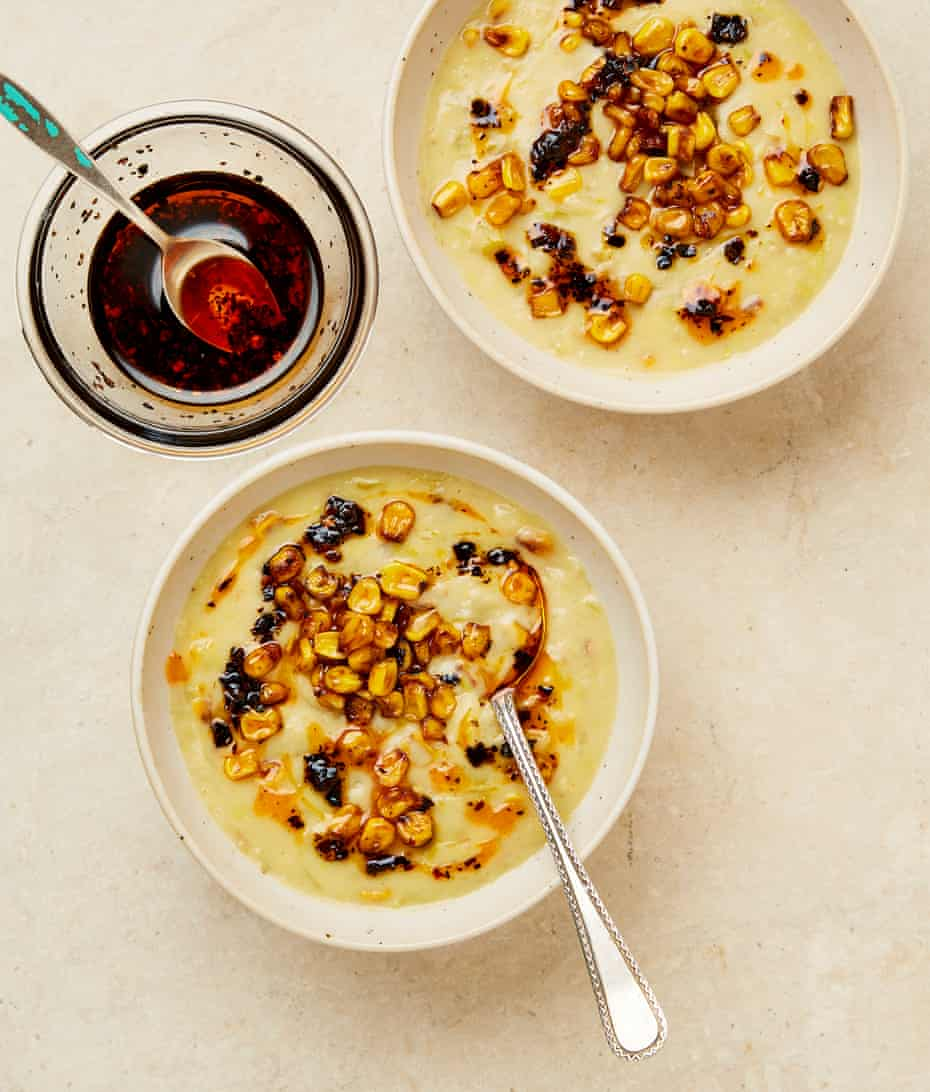
\includegraphics[width=10cm,height=10cm,keepaspectratio]{Recipe_Pictures/Sweetcorn_chowder_with_smoky_chipotle_oil.png}
\end{figure}
\emph{Back in the mists of time (from the 16th century onwards), French fishermen from Brittany travelled back and forth to Newfoundland in Canada to fish. At some point along the way, it’s thought their fish and potato stew cooked in a chaudière became American chowder. Today, chowder has splintered into many variations; some are made with tomatoes and others without any fish. My recipe borrows mostly from a New England variation made with sweetcorn, and is a perfect winter warmer. In it, potato offers velvet reassurance, sweetcorn pops with optimism, leeks and onion give sweet and savoury pungency and, for a bit of sparkle, there’s a salty smoky chipotle oil to finish.\\ 
I think this is a complete meal in itself, and doesn’t need anything else to accompany it. I’ve used frozen corn, but if you have tinned, drain a standard 198g tin to get 160g sweetcorn. You’ll need a blender.}\\\\ 
\textbf{Prep}: 15 min
\textbf{Cook}: 30 min
\textbf{Serves}: 4
\subsection*{Ingredients}
\begin{itemize}
\item 75ml rapeseed oil, plus 2 tbsp extra
\item 2 tbsp dried chipotle flakes
\item Fine sea salt
\item 200g frozen sweetcorn, defrosted
\item 2 leeks, trimmed and finely sliced (225g net)
\item 1 brown onion, peeled and finely sliced
\item 4 garlic cloves, peeled and grated
\item 500g potato, peeled and cubed into 1cm cubes
\item 2 tbsp vegetable bouillon, dissolved into 500ml water
\item 1 x 400ml can coconut milk
\item 1 tsp cider vinegar, or lemon juice
\end{itemize}

\subsection*{Steps}
\begin{enumerate}
\item Make the chipotle oil first. Heat the oil in a medium to large saucepan until hot, add the chipotle flakes and a half-teaspoon of salt, then take off the heat. Swirl, leave to cool a little, then carefully pour into a heatproof bowl to cool down further.
\item Add another tablespoon of oil to the same pan, if need be, and put it on a high heat. When very hot, add the sweetcorn in a single layer (if possible) and leave for two minutes to char slightly. Stir, leave undisturbed for another two minutes, until you see a good bit of colour, then tip into a medium bowl.
\item Add another tablespoon of oil to the pan, set it over a medium heat, then add the leeks and onion, and saute for eight minutes, until soft. Add the garlic, cook for two minutes, then add the potato, bouillon and three-quarters of a teaspoon of salt, and bring up to a boil. Turn down to a simmer and cook gently for 10 minutes, until the potato is cooked through and the tip of a knife slips in and out easily.
\item Return the sweetcorn to the pan (if you wish, reserve a small handful to decorate the soup), add the coconut milk and vinegar, bring back to a boil, then take off the heat.
\item Using a stick blender, blend the soup for 10-15 seconds, to thicken it a little (or ladle a third to a half of the soup into a blender, blitz, then pour back into the pan). Taste and adjust the seasoning, if need be, then ladle into bowls, sprinkle over the reserved corn, if using, drizzle with the smoky chipotle oil and serve.
\end{enumerate}
\newpage

\section{Lemon tart}
\begin{figure}
\centering
\includegraphics[width=10cm,height=10cm,keepaspectratio]{Recipe_Pictures/Lemon_tart.png}
\end{figure}
\emph{My theory is that everyone has a default pudding. My dad will always choose cheesecake, my daughter ice-cream, my husband loves a cheese plate and my best friend the chocolatiest thing on the menu. My weakness has always been lemon tart. Due to this lifelong love, I was sceptical that I’d be able to come up with a vegan take that would satisfy my own appetite, but here we are. In this recipe, silken tofu forms a rich base to overlay sharp winter lemons. It’s different from the traditional tart in that it’s fresher and brighter, so this is in no way a substitute, but another wonderful lemon tart in its own right.\\ 
You’ll need a loose-bottomed 24cm tart case and some blind baking beans (or dried beans) and a food processor. Any leftover lemons can be used to decorate the tart, as per the photo. The tart is best eaten on the day it’s made, or soon after.}\\\\ 
\textbf{Prep}: 20 min
\textbf{Cook}: 1 hr 10 min
\textbf{Chill}: 2 hr 30 min+
\textbf{Makes}: 1 x 24cm tart, to serve 8
\subsection*{Ingredients}
\begin{itemize}
\item For the pastry
\item 150g plain flour
\item 2 tbsp caster sugar
\item $\frac{1}{4}$ tsp fine sea salt
\item 75g vegan butter, cold
\end{itemize}

\begin{itemize}
\item For the curd filling
\item 2 x 300g packs silken tofu, drained (580g drained weight) – I like Clearspring
\item 7 lemons, zested and juiced, to get 240ml 
\item 200g caster sugar
\item 50ml soya milk
\item 4 tbsp cornflour
\item 100g vegan butter, melted
\item $\frac{1}{4}$ tsp turmeric
\end{itemize}

\subsection*{Steps}
\begin{enumerate}
\item For the pastry, in a food processor, pulse the flour, sugar and salt a few times, to combine. Add the butter, blitz for about a minute, add a tablespoon of water pulse just until the dough comes together, then stop – don’t over-process it, or the pastry will be tough. Tip out the dough on to a work surface, use your hands to bring it together into a a disc, then wrap in greaseproof paper and put in the fridge for at least 30 minutes.
\item Meanwhile, heat the oven to 190C (170C fan)/375F/gas 5. For the filling, put the tofu, lemon juice and zest, and the sugar in a food processor, and pulse to combine. Make a slurry with the soya milk and cornflour, then add this and the melted butter to the lemon mix and blitz to mix. Add the turmeric, blitz again, then scrape the filling into a jug and set aside while you blind bake the tart case.
\item Take the dough from the fridge and on a clean, floured work surface roll it out into a 32cm-diameter circle. Using the rolling pin to help you, carefully lift the pastry circle into the tart case, then, using your thumbs, gently help it into the edges and up the sides. Once lined, tear off a piece of baking paper large enough to cover the tart base with plenty of excess, lay it on top and fill the tart case with baking beans or similar. Blind bake for 15 minutes, then remove and check how the case is cooking: once the pastry is starting to look dry and pale beige in colour, lift out the paper and beans, and bake the case for another six minutes, until just starting to brown.
\item Pour the lemon mix into the blind-baked tart case, tap the tin on a flat surface to level out the filling and return to the oven for 30 minutes. After this time, the tart won’t look properly baked, but don’t be alarmed: just remove it from the oven, leave to cool to room temperature, then refrigerate for at least two hours, until the filling is set and the tart is ready to slice and serve.
\end{enumerate}
\newpage

\section{Miso and coconut winter greens}
\begin{figure}
\centering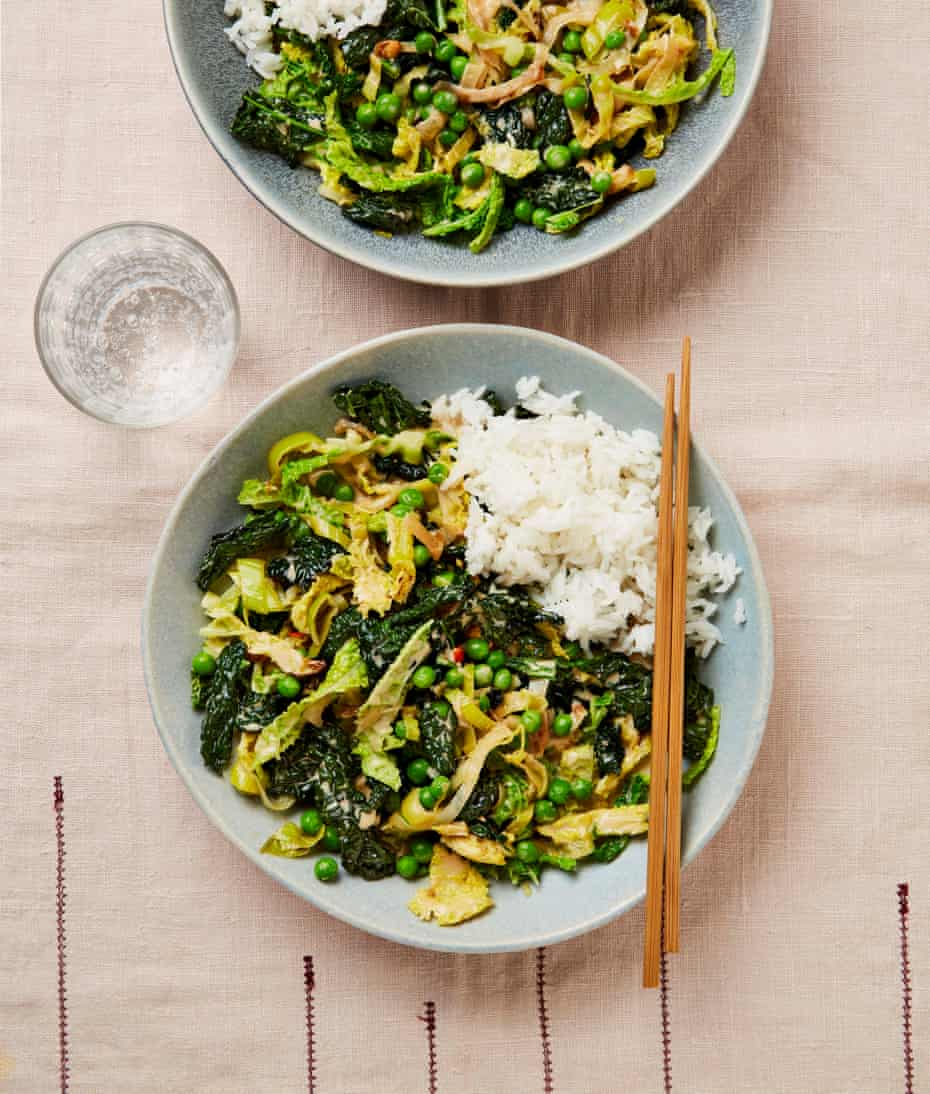
\includegraphics[width=10cm,height=10cm,keepaspectratio]{Recipe_Pictures/Miso_and_coconut_winter_greens.png}
\end{figure}
\emph{There’s something about chef Mary San Pablo, and that something is that she cooks some exceptionally fine food of Filipino origin, with an English lilt. She runs Luto, a pop-up but soon-to-be-permanent restaurant in east London, and it was there that I first ate laing, a dish of coconut milk-braised greens that’s traditionally made with taro leaves. Mary used kale, which she cooked to silky, flavourful submission (not words usually reserved for kale) and served over rice. I wrote this recipe because I had to eat it again before Mary’s restaurant opens, and really as a note to say, when it does open, go.\\ 
I use Clearspring brown rice miso, but any dark miso will do. Misos vary in potency and saltiness, with the darker ones being much more potent than the lighter-coloured, creamier and sweeter ones.}\\\\ 
\textbf{Prep}: 20 min
\textbf{Cook}: 40 min
\textbf{Serves}: 4
\subsection*{Ingredients}
\begin{itemize}
\item 3 tbsp rapeseed oil – I like Mr Organic
\item 1 large onion, peeled and finely sliced
\item 4 garlic cloves, peeled and crushed
\item 5cm x 5cm piece fresh ginger, peeled and grated
\item 4 red bird’s eye chillies, finely chopped
\item 250g leeks (about 2), trimmed and finely sliced
\item 400g kale or cavolo nero, ribs removed and saved for a stock or soup, leaves shredded
\item 400g savoy cabbage, cored and finely shredded
\item 250g frozen peas, defrosted
\item 2$\frac{1}{4}$ tbsp dark brown miso
\item 2 tbsp white-wine vinegar
\item $\frac{3}{4}$ tsp fine sea salt
\item 1 tbsp light soy sauce
\item 1 x 400ml tin coconut milk
\item Jasmine rice, to serve
\end{itemize}

\subsection*{Steps}
\begin{enumerate}
\item Put a large, deep-sided pot on the stove over a medium heat, add three tablespoons of oil and, once hot, add the onion and cook, stirring regularly, for 10 minutes, until soft and browning. Add the garlic, chillies and ginger, cook, stirring often, for three minutes, then add the leeks and cook for another five minutes.
\item Stir in the chopped kale – you may need to add it in batches, to allow the leaves to wilt a little – then cook, stirring occasionally, for five minutes. Add the savoy cabbage and cook for five minutes more, until the cabbage leaves are soft and bright green in colour.
\item Add the miso, vinegar, salt and soy to the pot, stir to mix in, then pour in the coconut milk. Fill the empty tin with water, add this to the pot, too, and bring everything to a boil. Pop in the peas, cook for a final three or four minutes, just to heat through, then take off the heat and serve hot over some freshly boiled rice.
\item  This article was amended on 16 January 2022 to correct a misspelling of Filipino in the headline.
\end{enumerate}
\newpage

\section{Leftover Christmas mixed fruit garibaldis}
\begin{figure}
\centering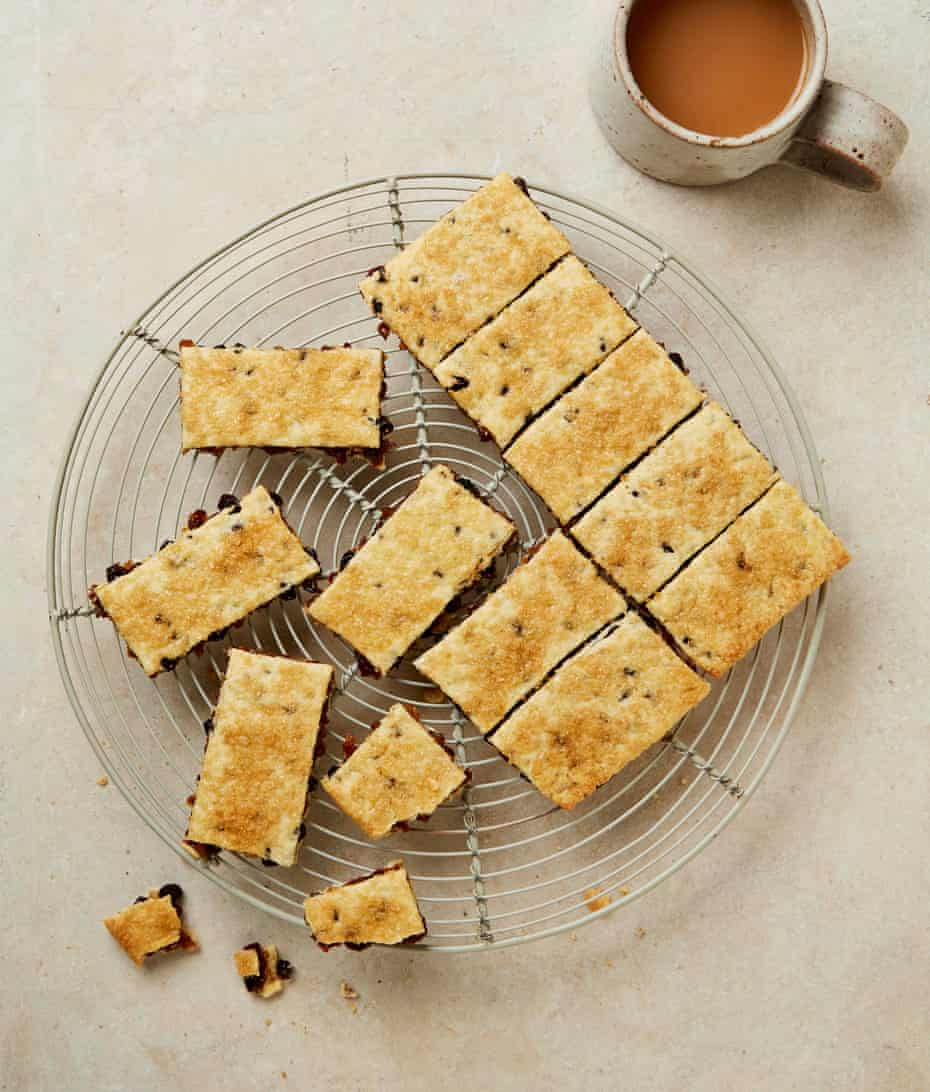
\includegraphics[width=10cm,height=10cm,keepaspectratio]{Recipe_Pictures/Leftover_Christmas_mixed_fruit_garibaldis.png}
\end{figure}
\emph{What you might not know about food writers is that we write our Christmas recipes as the sun sets on summer, long before the first rustle of tinsel is heard. As such, I’ve had an insight into what your store cupboard might look like post-Christmas and, if it’s anything like mine, you’ll currently have an assortment of dates, currants and other dried delights left over. Enter the legendary garibaldi biscuit: at 160 years old, not only is it still one of the finest biscuits to have been created, thanks to the delightful contrast of chewy raisins and crisp, brittle pastry, but it’s also a wonderful hoover-upper of your dried fruit odds and ends.\\ 
Don’t worry about using this exact combination of dried fruit; use the same amount of whatever you have to hand.}\\\\ 
\textbf{Prep}: 15 min
\textbf{Cook}: 50 min
\textbf{Rest}: 1 hr+
\textbf{Makes}: 20
\subsection*{Ingredients}
\begin{itemize}
\item For the biscuit dough
\item 220g strong white bread flour, plus extra for dusting
\item $\frac{1}{4}$ tsp fine sea salt
\item 50g caster sugar
\item 75g vegan butter, cubed
\item 5 tbsp oat milk, plus 1 tbsp extra for the glaze
\end{itemize}

\begin{itemize}
\item For the filling
\item 300g mixed dried fruit (I used 100g currants, 50g cranberries, 50g dates, 50g figs and 50g apricots), all finely chopped
\item 2 tbsp demerara sugar, plus 2 tsp extra for the glaze
\item 2 tbsp golden syrup
\item 2 tsp lemon juice
\item 2 tsp ground allspice
\end{itemize}

\subsection*{Steps}
\begin{enumerate}
\item In a food processor, blitz the flour, salt and sugar to mix. Add the butter and pulse until it is spread throughout the mix, but still in discernible pieces. Add the oat milk and pulse again, so the dough starts to come together. At this point, tip it out on to a floured work surface and push it together with your hands. Form into a rough block, wrap in baking paper and put in the fridge for at least an hour, to relax.
\item Heat the oven to 190C (170C fan)/375F/gas 5 and line a baking sheet (I have a reusable mat). Take the dough from the fridge and, using a couple of sheets of baking paper, or on a well-floured surface with a rolling pin, roll it out into a 40cm x 30cm rectangle with one of the short edges facing you. This pastry is short, and therefore crumbly, so go gently with the rolling pin, and push the edges together if need be.
\item Next, mix the dried fruit, demerara, golden syrup, lemon juice and allspice in a bowl, then tip out on to the half of the rolled-out dough that’s nearest to you. Use a knife or palette knife to help lift the remaining dough up and over the fruit mix towards you, so you’re left with a rectangle of filled biscuit dough. Roll this gently to return it to a roughly 35cm x 20cm rectangle, then cut it into 20 8cm x 4cm biscuits.
\item Lift the uncooked biscuits on to the lined tray, brush the tops with a little oat milk, then sprinkle over a little more demerara.
\item Bake in the hot oven for 20 minutes, until golden brown, then remove and leave to cool before eating.
\end{enumerate}
\newpage

\section{Kiri hodi with butternut squash}
\begin{figure}
\centering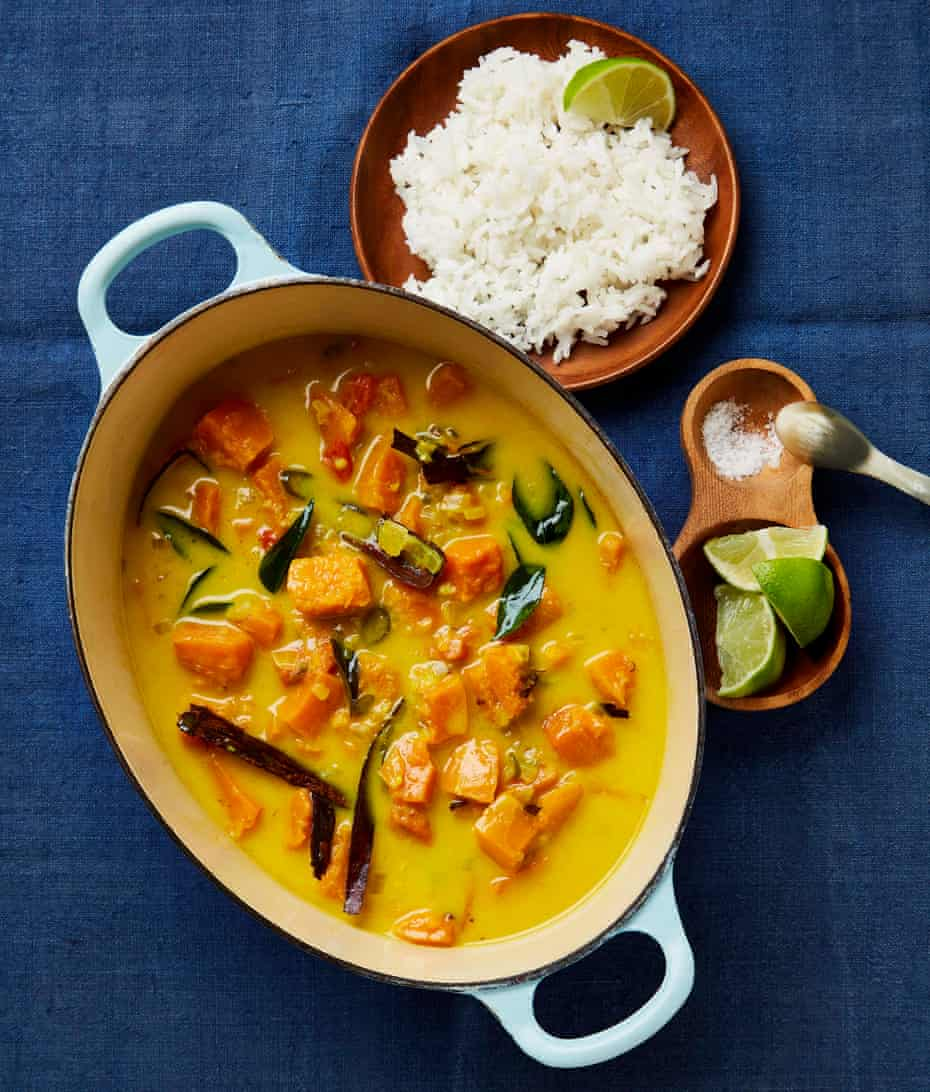
\includegraphics[width=10cm,height=10cm,keepaspectratio]{Recipe_Pictures/Kiri_hodi_with_butternut_squash.png}
\end{figure}
\emph{ Kiri hodi, or coconut milk curry, is one of Sri Lanka’s most popular dishes, and it is a genius recipe. All you need to do to create this taste of paradise, made using a combination of spices, aromats, citrus and coconut milk, is to bung the ingredients into a pot (largely all at the same time) and pop it on the stove. What joy. It’s the perfect thing to cook for time-poor or weary cooks, and the perfect thing to eat to bring some big tropical energy into your life.\\ 
The roast butternut is untraditional, but it lends its sweetness to the creamy sourness of kiri hodi. If you don’t have any, you could use almost any other vegetable instead. It’s worth hunting down fresh curry leaves; freeze any leftover leaves for next time.}\\\\ 
\textbf{Prep}: 15 min
\textbf{Cook}: 50 min
\textbf{Serves}: 4
\subsection*{Ingredients}
\begin{itemize}
\item 1kg butternut squash, halved, deseeded and peeled, flesh cut into 1$\frac{1}{4}$cm cubes (about 900g net)
\item 2 tsp mild curry powder
\item 1$\frac{1}{4}$ tbsp rapeseed oil
\item Fine sea salt
\item 1 brown onion, peeled and finely diced
\item 5 green finger chillies, finely sliced
\item 12-15 fresh curry leaves
\item $\frac{3}{4}$ tsp ground turmeric
\item $\frac{1}{4}$ tsp fenugreek seeds
\item 5 garlic cloves, peeled and crushed
\item 150g cherry tomatoes, halved
\item 1 x 10cm-long cinnamon stick, snapped in two
\item 2 x 400ml tins coconut milk
\item 1$\frac{1}{4}$ tbsp lime juice (ie from 1 lime)
\item Rice, to serve
\end{itemize}

\subsection*{Steps}
\begin{enumerate}
\item Heat the oven to 200C (180C fan)/390F/gas 6 and line a baking tray (I have a reusable baking liner).
\item Put the squash cubes in a large bowl, add the curry powder, rapeseed oil and three-quarters of a teaspoon of fine sea salt, and toss to coat. Tip out on to the tray in an even layer, roast for 35 minutes, then take out of the oven and set aside to cool.
\item Meanwhile, put the onion, chillies, curry leaves, turmeric, fenugreek, garlic, cherry tomatoes, cinnamon and one and a half teaspoons of salt in a medium saucepan, then add 200ml tap water. Over a medium to high heat, bring up to a boil and cook for 12 minutes, until the onions and tomatoes are completely soft and nearly all the liquid has evaporated. 
\item Add the coconut milk and the roast squash, bring back to a gently bubbling simmer, then turn off the heat and add the lime juice. Taste and adjust the salt and lime as needed, and serve with steamed rice.
\end{enumerate}
\newpage

\section{Gujarati whole mung dal with sambharo}
\begin{figure}
\centering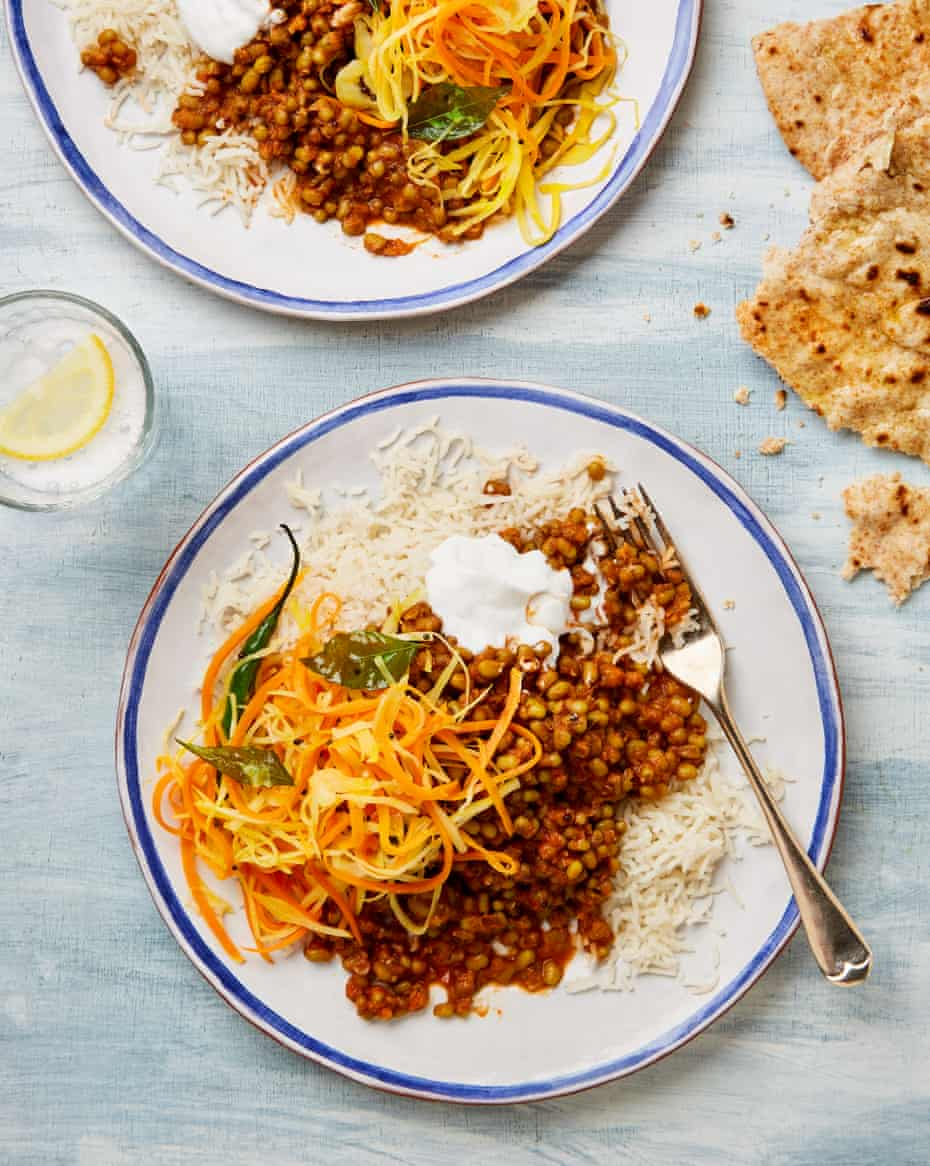
\includegraphics[width=10cm,height=10cm,keepaspectratio]{Recipe_Pictures/Gujarati_whole_mung_dal_with_sambharo.png}
\end{figure}
\emph{Mung beans are considered very lucky to the average Gujarati. These are the beans that their bones are built of, and not just because of their general prevalence. Mostly, they’re eaten wet like a dal, as in today’s dish, though sometimes they are dry-fried or sprouted with lots of garlic, cumin and lemon. Uncooked, they’re a popular bean at religious ceremonies – I still have a pocketful that were blessed at my wedding, as well as some from when I moved into my new house. Today, they are just here as an idea for dinner, but I wish you good luck in cooking them.\\ 
Traditionally, this is made without onions or garlic, making it a simpler and gentler dal, but it does need a perky sidekick, hence the sambharo, a sweet-and-sour relish, alongside. At home, Mum would serve this with wholemeal chapatis, but I eat it with steamed jasmine rice, which I make once I’ve set the dal on to simmer. This might look like a lot of ingredients, but they all go into the pan in quick succession and many from the dal overlap with those in the sambharo.}\\\\ 
\textbf{Prep}: 10 min
\textbf{Cook}: 1 hr
\textbf{Serves}: 4
\subsection*{Ingredients}
\begin{itemize}
\item For the dal
\item 2 tbsp rapeseed oil
\item $\frac{1}{4}$ tsp cumin seeds
\item 1 tsp black mustard seeds
\item 400g passata, or crushed tinned tomatoes
\item 3cm piece fresh ginger (20g), peeled and finely grated
\item 1 finger chilli, finely chopped
\item 1 tsp ground coriander
\item 1 tsp ground cumin
\item 1$\frac{1}{4}$ tsp fine sea salt
\item 350g whole mung beans
\end{itemize}

\begin{itemize}
\item For the sambharo
\item 2 tbsp rapeseed oil
\item 1 tsp black mustard seeds
\item 2 finger chillies, slit lengthways
\item 6 fresh curry leaves
\item $\frac{1}{4}$ white cabbage (200g), finely shredded
\item 1 large carrot (200g), shredded with a julienne peeler or grated
\item $\frac{3}{4}$ tsp fine sea salt
\item 1$\frac{1}{4}$ tsp lemon juice
\item $\frac{1}{4}$ tsp sugar (or to taste)
\end{itemize}

\subsection*{Steps}
\begin{enumerate}
\item Heat the oil in a deep saucepan over a medium heat and, when hot, add the cumin and mustard seeds, and leave to pop for 20-30 seconds. Turn the heat right down and gently add the tomatoes to the pan – watch out, because the oil might spit. Crank the heat back up to medium, then cook, stirring, for five minutes, until the tomatoes bubble thickly. Stir in the ginger, chilli, ground coriander, cumin and salt, cook for two minutes more, then add the mung beans and 1.2 litres water. Bring to a boil, then turn down to a whisper and cook, stirring every now and then, for 45 minutes, until the beans are soft but not mushy.
\item While the dal is cooking, make the sambharo, which can happily sit around and be eaten at room temperature. Heat the oil in a frying pan and, when hot, add the mustard seeds, chillies and curry leaves, and let them crackle and pop for 30 seconds. Add the cabbage and carrot, stir-fry for five minutes, until the vegetables have wilted but still have some crunch, then add the salt, lemon juice and sugar. Taste and adjust the seasoning accordingly.
\item Serve the dal over rice or alongside chapatis with the sambharo and perhaps some non-dairy yoghurt on the side.
\end{enumerate}
\newpage

\section{Haggis kheema and tattie rotis}
\begin{figure}
\centering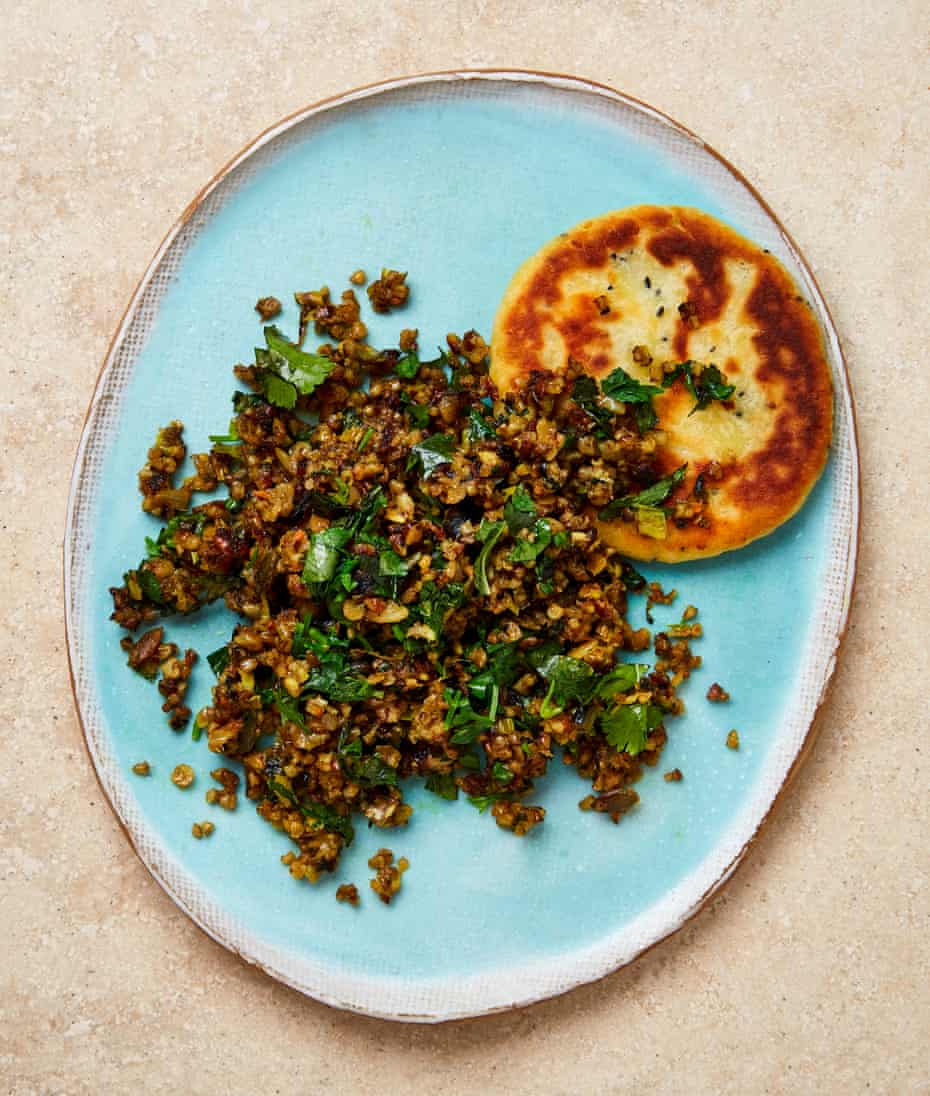
\includegraphics[width=10cm,height=10cm,keepaspectratio]{Recipe_Pictures/Haggis_kheema_and_tattie_rotis.png}
\end{figure}
\emph{Burns Night and my birthday are on the same day, which, over the years, has been both a blessing and a curse – a curse in that I haven’t always wanted to eat haggis, neeps and tatties or read poetry on 25 January, and a blessing in that there’s always been a pre-set suggestion on the birthday party idea-o-meter that’s more interesting than the usual: “Pub?” In any case, this year I am embracing it fully, merging Burns’ love for haggis and tatties with my love of Indian kheema and rotis, and so forming the inaugural Burns-Sodha birthday meal of haggis kheema and tattie rotis.\\ 
Treat the haggis and roti recipes separately, if you wish (and if you’re short of time, you could always buy wheat rotis). The dish is built around Macsween’s vegetarian haggis, which you’ll need to buy – it’s widely available in most supermarkets.}\\\\ 
\textbf{Prep}: 20 min
\textbf{Cook}: 1 hr 10 min
\textbf{Serves}: 4
\subsection*{Ingredients}
\begin{itemize}
\item For the tattie rotis
\item 300g maris piper potatoes, peeled and cut into 3cm cubes (250g net weight)
\item 1 tbsp rapeseed oil, plus 1 tsp extra for frying the rotis
\item Salt
\item $\frac{1}{4}$ tsp nigella seeds
\item 125g plain white flour, plus extra for dusting
\end{itemize}

\begin{itemize}
\item For the haggis kheema 
\item 3 tbsp rapeseed oil
\item 1 medium leek (250g), finely sliced
\item 1 large onion, peeled and finely chopped
\item 2cm piece fresh ginger, peeled and grated
\item 5 garlic cloves, peeled and minced
\item 2 Indian green finger chillies, very finely chopped
\item 1kg vegan haggis
\item 2 tsp ground coriander
\item 2$\frac{1}{4}$ tsp ground cumin
\item $\frac{1}{4}$ tsp turmeric
\item 100g non-dairy yoghurt – I like Coconut Collaborative
\item 1 large handful (10g) fresh mint leaves, chopped
\item 1 large handful (15g) fresh coriander leaves, chopped
\end{itemize}

\subsection*{Steps}
\begin{enumerate}
\item Bring a small pan of water to a rolling boil, drop in the potatoes and cook for 12 minutes, or until tender. Drain and leave to dry in the colander. When dry, put the cooked potatoes back into the same pan, add the oil, half a teaspoon of salt and the nigella seeds, and mash really well. Add the flour and knead with your hands until the mix comes together into a uniform ball of dough.
\item Lightly flour a work surface and lay out a large sheet of greaseproof paper. Cut the roti dough into four equal pieces. Take one piece of dough, roll it out into a 6cm-diameter circle (dip the rolling pin in flour if need be), then transfer to the paper and repeat with the remaining dough.
\item Heat a teaspoon of oil in a large, nonstick frying pan and, when hot, lay in the rotis and cook for about a minute and a half on each side, until blackened in places and there are no uncooked, doughy spots – as the pan starts to heat up, the roti will cook more quickly, so you may need to reduce the cooking time and/or heat. Cover the cooked rotis with foil and set aside while you make the kheema.
\item In the same frying pan, heat the oil for the kheema over a medium heat. When hot, add the leek and onion, and cook for about eight minutes, until soft and translucent. Add the ginger, garlic and chillies, stir to mix and cook for two minutes more.
\item Crumble in the haggis and cook, stirring frequently, for about eight minutes – it may stick to the pan, but persevere. Stir in the ground coriander, cumin, turmeric and yoghurt, cook for a further four minutes, then taste for seasoning. Add salt a quarter-teaspoon at a time, mixing and tasting after each addition, then stir in the fresh herbs and serve hot with the rotis.
\end{enumerate}
\newpage

\section{Hoppin’ John}
\begin{figure}
\centering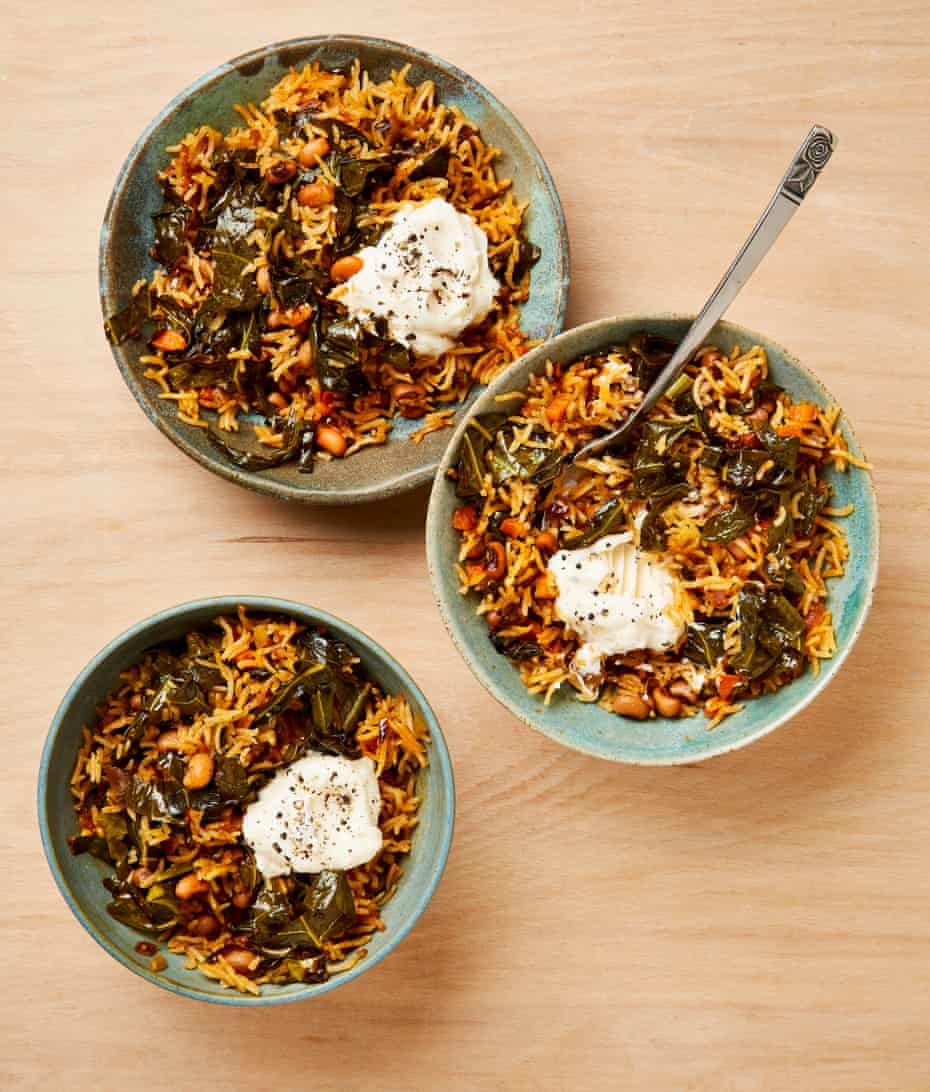
\includegraphics[width=10cm,height=10cm,keepaspectratio]{Recipe_Pictures/Hoppin_John.png}
\end{figure}
\emph{Hoppin’ John is traditionally eaten in the southern states of the US, and comprises rice and black-eyed beans cooked together, much like a pilau, and served with collard greens. Eating it on New Year’s Day is said to bring luck and prosperity – the beans represent coins, the greens dollar bills – and although we’re long past that, it could certainly save you money, because it’s a wildly economical meal. My recipe is a broad interpretation of the original: I’ve cooked the greens with the rice and thrown in an old family favourite ingredient, Tabasco. The result is a gentle, soothing, belly-warming dish with a small vinegar kick to it.\\ 
So that you don’t get ambushed by the recipe, do all the chopping up front, then it is just a question of throwing things into a pan. You’ll need a large frying pan with a tight fitting lid.}\\\\ 
\textbf{Prep}: 20 min
\textbf{Cook}: 40 min
\textbf{Serves}: 6-8
\subsection*{Ingredients}
\begin{itemize}
\item 4 tbsp groundnut oil
\item 1 red onion, peeled and finely diced
\item 2 carrots (about 200g) finely diced
\item 3 celery stalks (about 200g), finely diced
\item 3 garlic cloves, peeled and minced
\item 1 tbsp tomato puree
\item 1 $\frac{1}{4}$ tbsp Tabasco 
\item 200g spring greens, shredded
\item 300g basmati rice, washed and drained
\item 1 x 400g tin black-eyed beans, drained
\item 550ml vegetable stock (suitable for vegans)
\item 1 tsp fine sea salt
\item Vegan garlic mayonnaise, to serve
\end{itemize}

\subsection*{Steps}
\begin{enumerate}
\item Put the oil in a deep-sided frying pan for which you have a tight fitting lid, and set it over a medium heat. When the oil is hot, add the diced onion, carrot and celery, and cook, stirring every now and then, for 20 minutes, until everything has sweated down and started to caramelise. Add the garlic, tomato puree and Tabasco, and cook, stirring regularly, for five minutes more.
\item Add the spring greens to the pot, stir to mix, then leave to wilt down. Add the rice, drained beans, stock and salt, stir and bring up to a boil. Turn down the heat to a whisper, then pop on the lid and leave to simmer for 15 minutes. Turn off the heat and leave to rest for 10 minutes without lifting the lid.
\item Distribute into bowls and serve with a big blob of garlic mayonnaise on top.
\end{enumerate}
\newpage

\section{Apple pudding cake}
\begin{figure}
\centering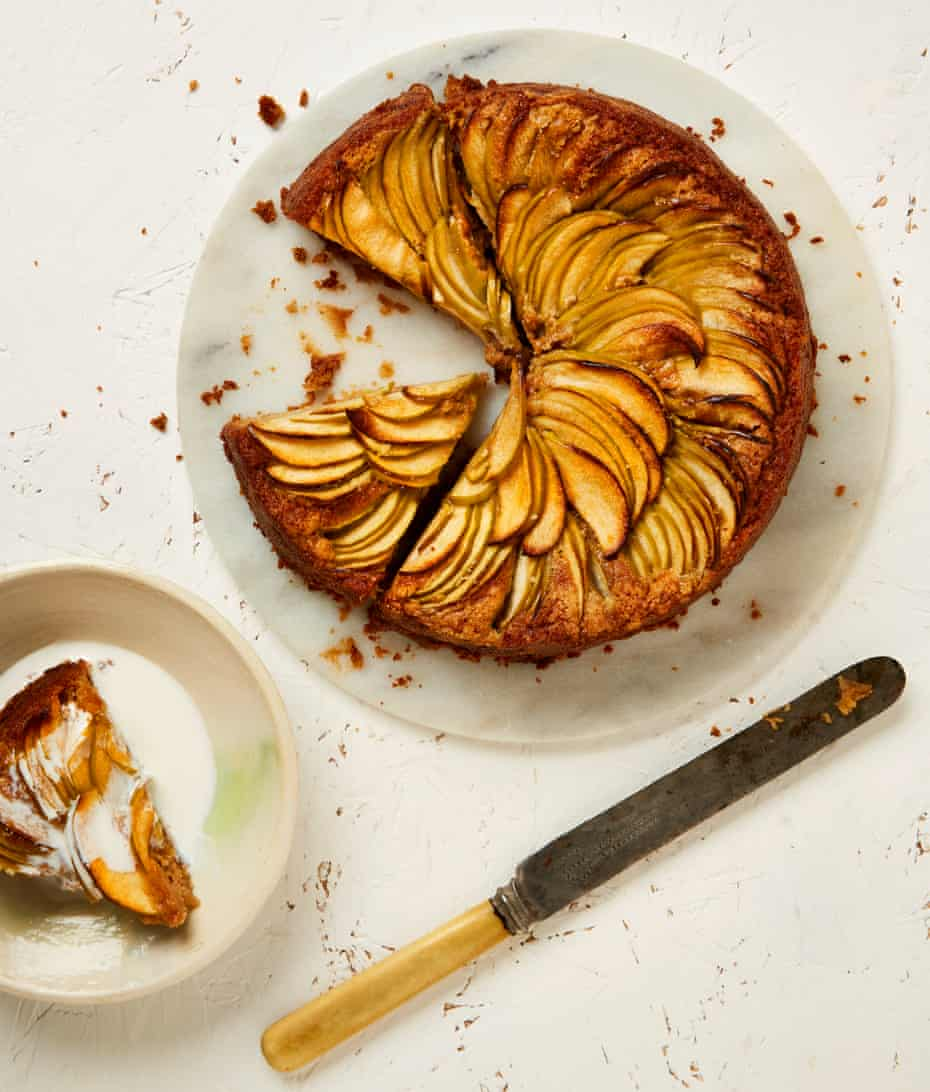
\includegraphics[width=10cm,height=10cm,keepaspectratio]{Recipe_Pictures/Apple_pudding_cake.png}
\end{figure}
\emph{Some time ago, when my daughter was nearly two, we took a walk and the sky sprung a leak. We should have known better (ie checked a weather app). We were on the knife-edge of a meltdown with a tired and soggy toddler when we spotted a table at E5 Bakehouse in Hackney, east London, and shared a slice of the most beautiful apple cake. It had enough apple in it to be potentially good for you, a crunchy demerara top and soft, puddingy insides. Such was its power that we forgot how sodden we were and, looking back, that day was a sort of heaven. Today’s recipe is my approximation of that wonderful cake.}\\\\ 
\textbf{Prep}: 15 min
\textbf{Cook}: 1 hr 10 min
\textbf{Serves}: 8-10
\subsection*{Ingredients}
\begin{itemize}
\item For the apples
\item 2 granny smith apples, peeled, cored and cut into 2cm cubes (175g prepared weight)
\item 1$\frac{1}{4}$ tsp ground cinnamon
\item 40g soft brown sugar
\end{itemize}

\begin{itemize}
\item For the cake batter
\item 200g self-raising flour
\item 1$\frac{1}{4}$ tsp baking powder
\item $\frac{1}{4}$ tsp salt
\item 160g soft brown sugar
\item 120ml olive oil
\item 1 tsp vanilla extract
\item 100ml non-dairy milk (I used oat)
\item 1 tbsp apple cider vinegar
\end{itemize}

\begin{itemize}
\item For the top of the cake
\item 2 granny smith apples, cored and sliced
\item 1 tbsp soft brown sugar
\end{itemize}

\subsection*{Steps}
\begin{enumerate}
\item Heat the oven to 200C (180C fan)/390F/gas 6, and line a 20cm springform round cake tin with greaseproof paper.
\item In a medium bowl, mix the apple cubes with the cinnamon and brown sugar, and set aside.
\item Measure all the dry ingredients for the batter into a large bowl, stir to combine, then pour in the wet ingredients and beat until you have a smooth batter. Tip in the cubed apples and their sugary, cinnamony juices, stir to combine, then scrape the batter into the lined tin.
\item Fan the sliced apples in a circle to cover the top of the cake, sprinkle over the remaining soft brown sugar, then bake on the middle shelf of the oven for 50-60 minutes, until the cake has risen, the apples on top are golden and a skewer inserted into the centre comes out clean. Serve warm or cold.
\end{enumerate}
\newpage

\section{Spiced beetroot with 60-minute injera}
\begin{figure}
\centering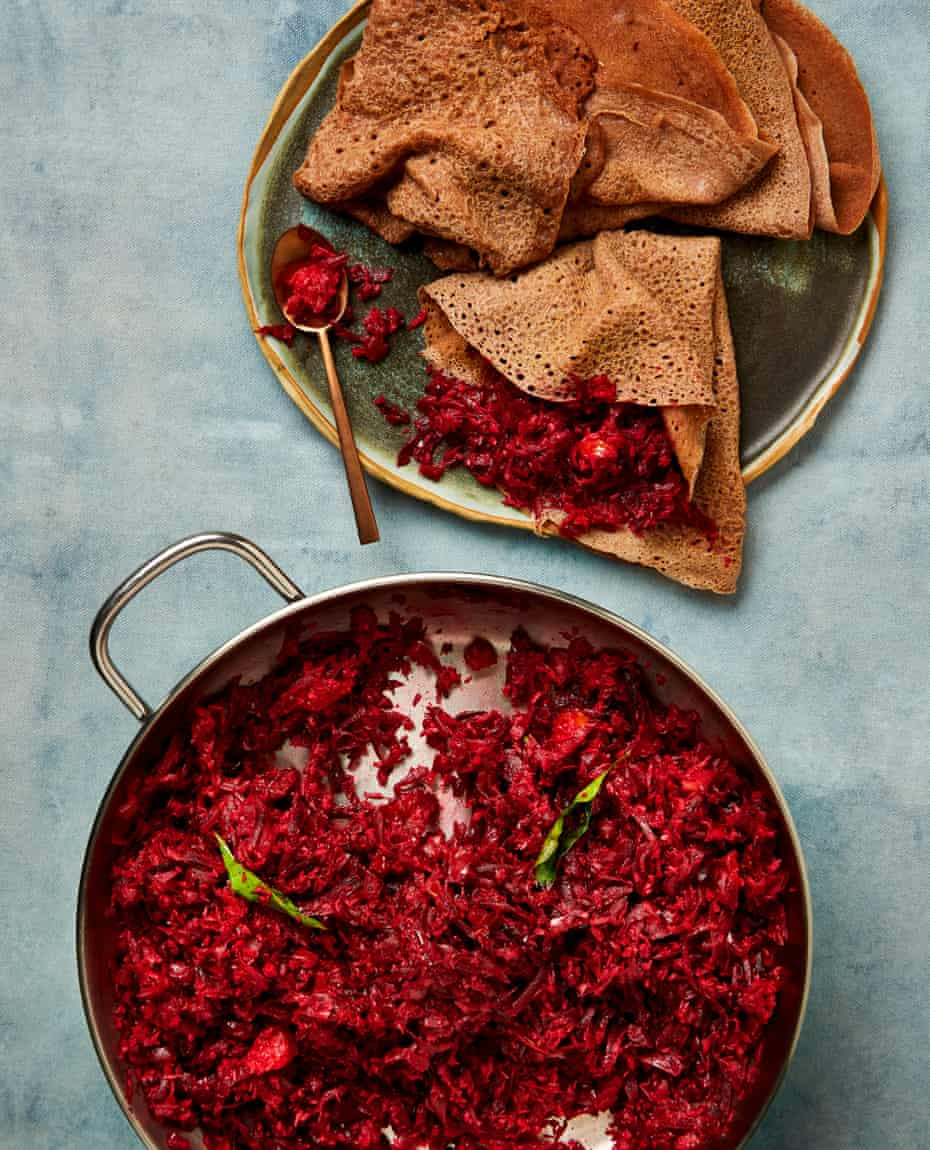
\includegraphics[width=10cm,height=10cm,keepaspectratio]{Recipe_Pictures/Spiced_beetroot_with_60-minute_injera.png}
\end{figure}
\emph{Injera is a fermented Ethiopian flatbread with a pleasing, sour flavour and a spongy, sauce-soaking texture. As with other fermented breads (such as sourdough and dosa), injera dough usually requires a starter culture, which can take days. Today’s recipe is the cheat’s version, soured with yeast and vinegar, which is still very satisfying to eat and make, but not quite the same as the original. Injera is usually eaten with misir wot, or spiced lentils, but this sweet spiced beetroot also works very well with the sourness of injera.\\ 
You can find teff flour in healthfood stores, online and in specialist food stores. You’ll need a good nonstick pan with a lid to cook the injera.}\\\\ 
\textbf{Prep}: 15 min
\textbf{Cook}: 25 min
\textbf{Rest}: 1 hr
\textbf{Serves}: 4
\subsection*{Ingredients}
\begin{itemize}
\item For the injera
\item 250g teff flour
\item 80g plain flour
\item 7g dried yeast
\item 1 $\frac{1}{4}$ tsp fine sea salt
\item 2 $\frac{1}{4}$ tbsp cider vinegar
\item Rapeseed oil
\end{itemize}

\begin{itemize}
\item For the beetroot
\item 2 tbsp rapeseed oil
\item 6 fresh curry leaves
\item 1 tsp black mustard seeds
\item $\frac{1}{4}$ tsp cumin seed
\item 1 onion, peeled and finely chopped
\item 3 garlic cloves, peeled and minced
\item 1 finger chilli, finely chopped
\item 2 medium tomatoes, roughly chopped
\item 500g beetroot, peeled and grated
\item 1$\frac{1}{4}$ tsp fine sea salt
\item 50g desiccated coconut (or 10 tablespoons)
\end{itemize}

\subsection*{Steps}
\begin{enumerate}
\item Put the teff, plain flour and yeast in a large bowl, add 400ml hand-hot water (I add 150ml freshly boiled water to 250ml cold tap water), then beat with an electric whisk for a couple of minutes, until lump-free and creamy. Cover with a tea towel and leave for an hour, in which time it should rise nicely.
\item In the meantime, cook the beetroot. Heat the oil in a frying pan over a medium to high heat and, once hot, add the curry leaves, mustard seeds and cumin seeds. Cook for a minute, until the seeds pop, then add the onion and fry for five minutes, until soft. Add the garlic and chilli, cook, stirring, for a further three minutes, then add the tomatoes, beetroot and salt. Cook until the water evaporates and the mixture turns quite dry, which should take about six minutes, then stir through the coconut. Take off the heat and leave to one side while you make the injera.
\item Add 200ml warm water (straight from the tap is fine) to the risen injera batter along with the salt and vinegar, and mix to combine. Rub the surface of a nonstick pan with oil using kitchen paper, then set it over a medium heat. Keep a spatula and a plate to hand. Add a ladleful of batter to the pan, swirl it around into a circle and wait until the “eyes” (ie, the little holes) have mostly disappeared and the batter has turned dark brown (around 30 seconds). Put a lid over the top of the pan for a minute, until the whole injera has turned darker (around another 30 seconds), then lever out of the pan and on to the plate, and keep warm. Add a drop more oil to the pan, if need be, and repeat with the remaining batter.
\item To serve, gently warm up the beetroot, bring everything to the table and let people serve themselves, tucking a spoonful of the beetroot into a folded injera.
\end{enumerate}
\newpage

\section{Most popular}
\begin{figure}
\centering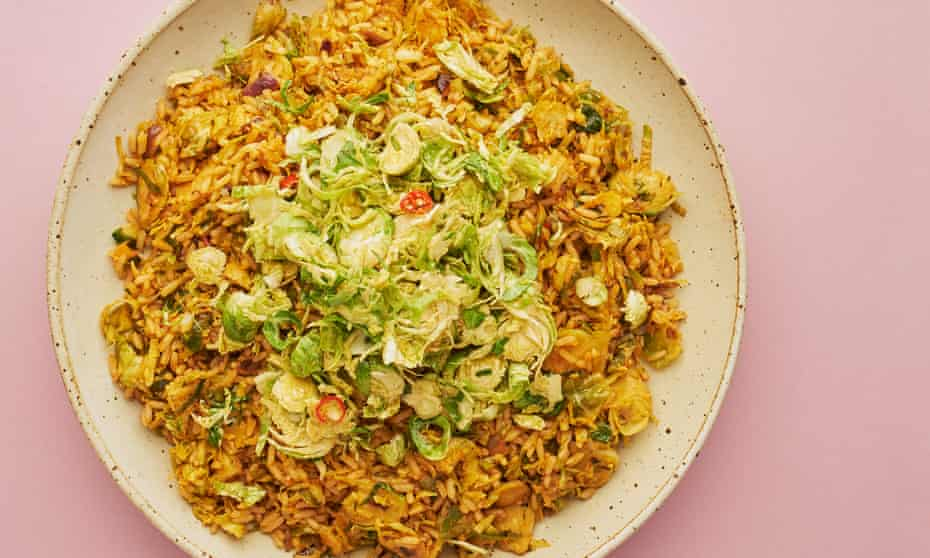
\includegraphics[width=10cm,height=10cm,keepaspectratio]{Recipe_Pictures/Most_popular.png}
\end{figure}
\emph{Sometimes, all you really want is something with that sort of filthy and delicious taste that I used to think only a good takeaway could provide – until I accidentally recreated it while writing this recipe for Malaysian nasi goreng. It’s fried rice, but not as you know it: smothered in unami-ific sauces, and topped with shredded, marinated sprouts for crunch and zing. All the joy of a takeaway, but without the wait or delivery charge.\\ 
Kecap manis is a sweet soy sauce that can be found in larger supermarkets, online and in south-east Asian food shops. I cut the sprouts by hand, but you could use the slicing attachment on a food processor.}\\\\ 
\textbf{Prep}: 10 min
\textbf{Cook}: 30 min
\textbf{Serves}: 4
\subsection*{Ingredients}
\begin{itemize}
\item 350g jasmine rice
\item 3 tbsp rapeseed oil 
\item 1 red onion, peeled and chopped 
\item 4 garlic cloves, peeled and crushed 
\item 3 bird’s eye chillies, very finely chopped (deseeded, if you prefer less heat)
\item 750g brussels sprouts, very finely sliced 
\item 2 tbsp tomato puree
\item 2 tbsp kecap manis
\item 1 $\frac{1}{4}$ tsp salt
\item 2 tbsp soy sauce 
\item 1 tbsp white-wine vinegar 
\item 2 tbsp toasted sesame oil 
\item 1 tsp sugar
\end{itemize}

\subsection*{Steps}
\begin{enumerate}
\item Put the rice in a sieve and wash under the cold tap until the water runs clear. Tip the rice into a pan, add 500ml fresh cold water and bring to a boil. Turn down the heat to a whisper, cover the pan and leave to cook for 15 minutes. Turn off the heat and leave with the lid still on, to steam through.
\item To cook the nasi goreng base, heat the rapeseed oil in a large frying pan on a medium flame and, when hot, fry the onion, stirring, for five minutes. Add the garlic and two-thirds of the chopped chillies, cook for two minutes more, then add all but two large handfuls (or about 150g) of the sprouts. Fry for eight minutes, leaving them undisturbed for a couple of minutes at a time, so they get some colour on them. Then stir in the tomato puree, kecap manis, salt and a tablespoon each of soy sauce and vinegar. Cook for another five minutes, then take off the heat.
\item To make the marinated sprouts, put the remaining raw sliced sprouts in a bowl with the soy sauce, white-wine vinegar, toasted sesame oil, sugar and the remaining chopped chilli. Mix very well and set aside.
\item To finish the nasi goreng, put the sprout and onion pan on a medium heat and gently scoop in the steamed rice, folding it in until well mixed. Heat through, stirring gently, for five minutes, until the rice is nice and hot, and season to taste. Transfer to a big platter, scatter the marinated sprouts over the top and serve.
\item Photography: Rob White. Food stylist: Amy Stephenson.
\end{enumerate}
\newpage

\section{Masala baked beans on toast with green chutney}
\begin{figure}
\centering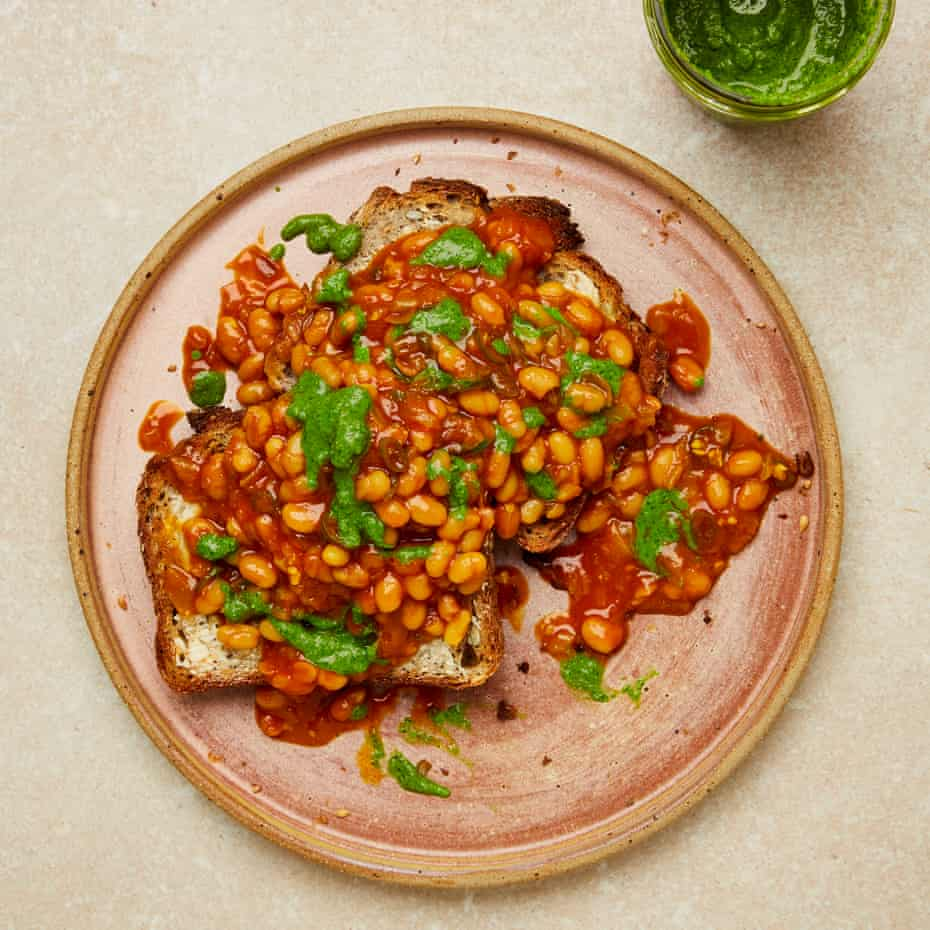
\includegraphics[width=10cm,height=10cm,keepaspectratio]{Recipe_Pictures/Masala_baked_beans_on_toast_with_green_chutney.png}
\end{figure}
\emph{My mother grew up in relative wealth in Uganda, but entered into poverty when she and her family arrived in the UK after being exiled by the dictator Idi Amin. \\ 
Having little money meant cooking very thriftily: she made chutney from fallen apples in the garden, bought sacks of lentils and rice from wholesalers, and ate a lot of spiced masala baked beans. \\ 
I am by no means poor, but this time in January (post-Christmas, pre-payday) can be very testing, and these beans are some of the most frugal but delicious things a person can eat.\\ 
Eat these for breakfast, lunch or dinner, on toast or with chapatis, and with or without a little non-dairy yoghurt or the green chutney. This makes enough beans to top two slices of toast generously, so double it to serve more.}\\\\ 
\textbf{Prep}: 10 min
\textbf{Cook}: 20 min
\textbf{Serves}: 2
\subsection*{Ingredients}
\begin{itemize}
\item For the beans 
\item 2 tbsp rapeseed oil 
\item 1 large brown onion, peeled and finely chopped
\item 2 garlic cloves, peeled and minced 
\item 1$\frac{1}{4}$ green finger chillies 
\item 1 heaped tsp tomato puree
\item 1 tsp ground coriander 
\item $\frac{1}{4}$ tsp ground turmeric 
\item $\frac{1}{4}$ tsp ground cumin 
\item $\frac{1}{4}$ tsp fine sea salt 
\item 1 x 400g tin Heinz baked beans
\end{itemize}

\begin{itemize}
\item For the chutney
\item 60g coriander (leaves and tender stalks) 
\item 1$\frac{1}{4}$ green finger chillies 
\item 2 tbsp fresh lemon juice 
\item $\frac{1}{4}$ tsp fine sea salt 
\item 2 tbsp rapeseed oil 
\item 2 tbsp roasted salted peanuts
\end{itemize}

\begin{itemize}
\item To serve
\item 2 slices good bread
\item Non-dairy spread
\end{itemize}

\subsection*{Steps}
\begin{enumerate}
\item Make the chutney first. Put the coriander in a bowl, add cold water to cover and agitate with your hand. Fish out the coriander and put it into a colander, leaving behind any gritty bits. Roughly chop the drained coriander, then throw it into a blender with the chillies, lemon juice, salt, oil and peanuts, and blitz to a smooth chutney (the coriander, being wet, will help it blend), adding a drop of water, if need be. Taste and adjust the lemon, salt and chilli as you wish – this chutney should be sour, herbal and hot – then scrape into a bowl and leave to one side.
\item To cook the beans, heat the oil in a frying pan and, once it’s hot, add the onion and cook, stirring regularly, for 10 minutes, until soft, golden and translucent. Add the garlic and chilli, cook, stirring, for three minutes more, then add the tomato puree, all the spices and the salt. Cook for two minutes, then add the beans and a half-tin’s worth of water, and cook for five minutes, until the sauce has thickened a little, then turn off the heat.
\item Toast the bread and put on two plates, spread generously with your favourite spread, pile the beans on top and decorate Jackson Pollock-style with the coriander chutney, or just spoon it over, as you wish.
\end{enumerate}
\newpage

\section{Tofu katsu sando with celeriac and apple slaw}
\begin{figure}
\centering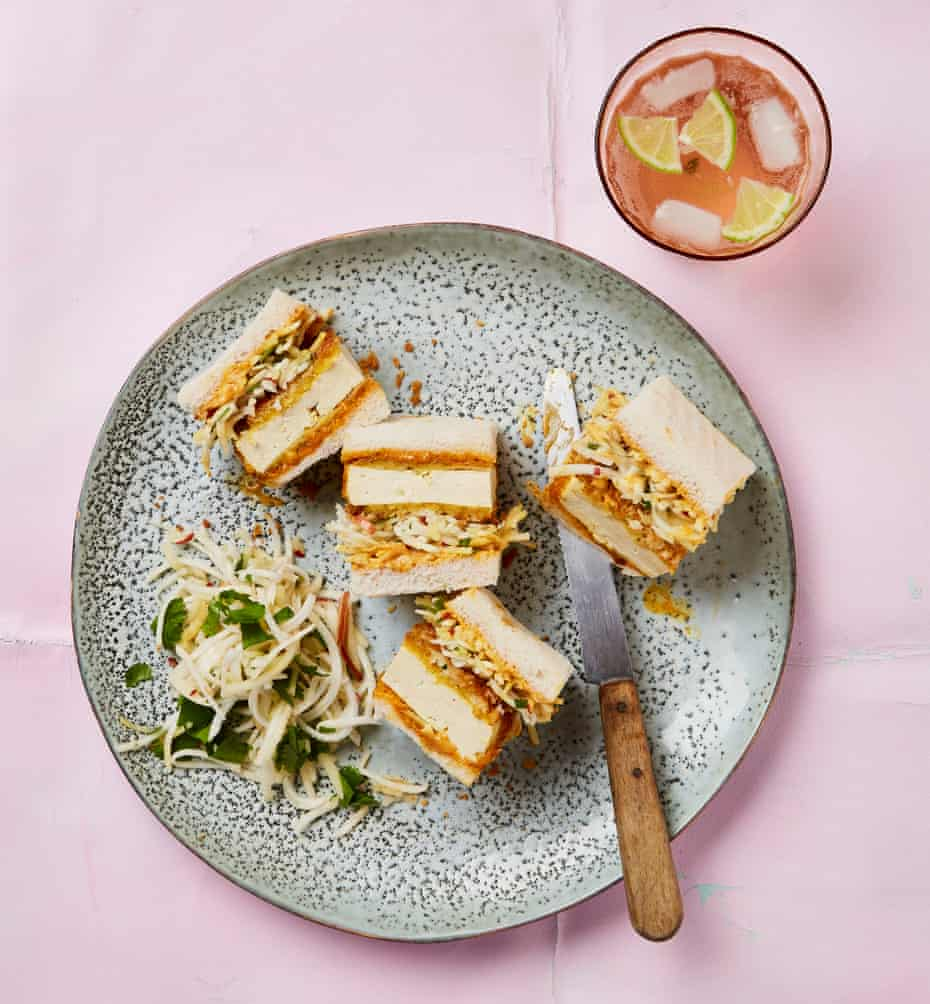
\includegraphics[width=10cm,height=10cm,keepaspectratio]{Recipe_Pictures/Tofu_katsu_sando_with_celeriac_and_apple_slaw.png}
\end{figure}
\emph{My life can be carved into two parts: a time before katsu sando and the enlightened after period. \\ 
It’s hard for a sandwich, the lunchtime stalwart, to break ranks and become exciting and even famous, but it’s easy to see how this Japanese take on it has done just that. \\ 
Here, a tofu cutlet is coated with panko breadcrumbs, fried until crisp, then slathered with curried ‘mayo’. Then it’s covered in an eye-opening celeriac and apple slaw before being sandwiched between the softest bread available. It’s carb-on-carb action, and a satisfying sandwich of contrasts.\\ 
In January, when UK-grown veg is not very abundant, tofu is a brilliant store-cupboard ingredient to have at your disposal, though cooked, breaded and fried pumpkin/squash or aubergine would also make great fillings. If you have one, use a food processor with the right slicer blade to matchstick the apple and celeriac, or a julienne peeler.}\\\\ 
\textbf{Prep}: 25 min
\textbf{Cook}: 30 min
\textbf{Serves}: 4
\subsection*{Ingredients}
\begin{itemize}
\item $\frac{1}{4}$ large celeriac (250g) peeled and cut into matchsticks
\item 2 medium apples (about 200g), core removed and cut into matchsticks
\item 2 tbsp rice-wine vinegar
\item 1$\frac{1}{4}$ tsp fine sea salt
\item 2 tbsp coriander leaves, roughly chopped
\item 8 tbsp vegan mayonnaise (I like Leon’s) 
\item 2 tbsp tomato ketchup 
\item 4 tsp medium curry powder 
\item 2 x 280g packs extra-firm tofu
\item 50g panko breadcrumbs 
\item Sunflower or rapeseed oil, for frying 
\item 8 slices white bread
\end{itemize}

\subsection*{Steps}
\begin{enumerate}
\item In a medium bowl, toss the celeriac and apple with the vinegar, a teaspoon of salt and the coriander, then leave to soften. In a small bowl, whisk half the mayo with the ketchup, two teaspoons of curry powder and a quarter-teaspoon of salt. 
\item Drain the tofu, squeezing out any moisture with your hands, then pat dry with kitchen paper. Cut each block horizontally into four “steaks”, to give eight in all. Put the rest of the mayo, curry powder and a quarter-teaspoon of salt into a shallow bowl, add a tablespoon of warm water and stir to loosen. Put the panko on a lipped plate.
\item One by one, cover both sides of the tofu steaks in the curried mayo, shake off any excess, then press into the panko to coat, and lay on an oven tray. Pour $\frac{1}{4}$cm oil into a high-sided, nonstick frying pan and put on medium heat until simmering. Fry half the panko-coated tofu steaks for a minute and a half on each side, until crisp and golden, then transfer to a plate lined with kitchen paper to drain. Repeat with the rest of the tofu.
\item Spread half the curried mayo on four slices of bread. Lay two tofu steaks on top of each slice and top with slaw. Spread the rest of the mayo on the other slices of bread and place on top, mayo side down. Using a bread knife, cut away the crusts, so the bread is the same size as the tofu, then cut each sandwich into four and serve with extra slaw on the side.
\end{enumerate}
\newpage

\section{Cauliflower and sweet potato tacos with coriander chilli salsa}
\begin{figure}
\centering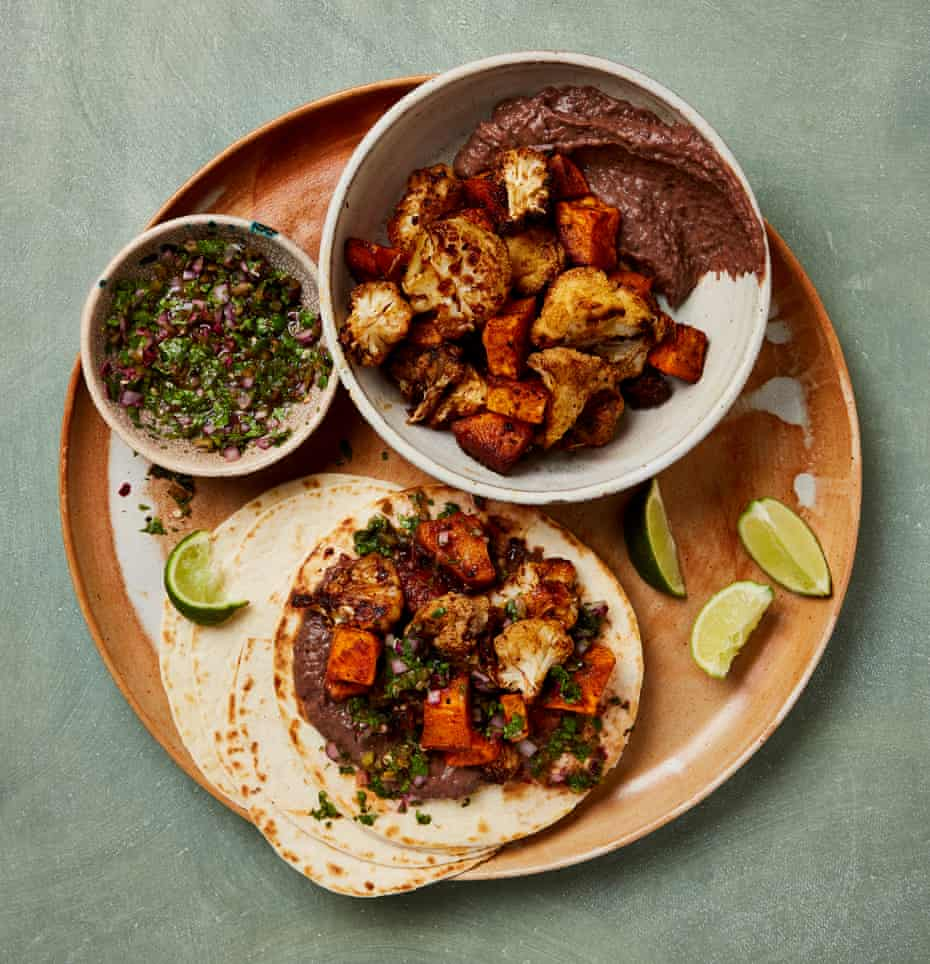
\includegraphics[width=10cm,height=10cm,keepaspectratio]{Recipe_Pictures/Cauliflower_and_sweet_potato_tacos_with_coriander_chilli_salsa.png}
\end{figure}
\emph{When I was growing up, I wanted to be Sam from the sci-fi series Quantum Leap, travelling through time to wake up in a new city with a new adventure. In 2015, I got a chance to feel a bit like him while on a north American book tour: in New York, I met Madhur Jaffrey; in Toronto, I got lost in vast Asian markets; and in San Francisco, I danced at a block party and ate tacos in the Mission district. They practically vibrated in my hands with flavour and personality, from the zingy salsa and the spicy vegetables to the hot, soft tortillas. Which are just the sort of vibrations I need now, in January 2020.\\ 
You don’t have to char the chillies for the salsa, but it gives them a milder, smokier and more rounded flavour. Tortillas vary in size and quality – my preference is for smaller, hand-sized ones such as those from Gran Luchito.}\\\\ 
\textbf{Prep}: 15 min
\textbf{Cook}: 40 min
\textbf{Makes}: 12, to serve 4
\subsection*{Ingredients}
\begin{itemize}
\item For the coriander chilli salsa 
\item 2 jalapeño chillies 
\item $\frac{1}{4}$ red onion, chopped into $\frac{1}{4}$cm dice 
\item 50g coriander leaves, very finely chopped
\item 4 tbsp fresh lime juice (ie, from 3 or 4 limes)
\item $\frac{3}{4}$ tsp fine sea salt
\end{itemize}

\begin{itemize}
\item For the roast vegetable filling 
\item 1 large cauliflower (about 800g), cut into small florets 
\item 1 large sweet potato (around 400g), peeled and cut into 2$\frac{1}{4}$cm pieces 
\item 5 tbsp rapeseed oil 
\item 2 tsp ground chipotle 
\item 2 tsp ground cinnamon 
\item 2 tsp fine sea salt
\end{itemize}

\begin{itemize}
\item For the black bean puree 
\item 1 x 400g tin black beans 
\item 1 tsp ground chipotle 
\item $\frac{1}{4}$ tsp fine sea salt 
\item 12 small tortilla wraps, to serve
\end{itemize}

\subsection*{Steps}
\begin{enumerate}
\item Heat the oven to 220C (200C fan)/425F/gas 7. To make the salsa, hold one of the chillies in a pair of tongs over a small gas flame until charred thoroughly (if you don’t have an open flame on the cooker, grill the chillies instead, until blackened), then put on a plate, repeat with the other chilli and leave to cool.
\item Put the onion, coriander, lime juice and salt in a small bowl. Once the chillies have cooled down, finely chop and mix into the salsa. Taste and adjust if need be.
\item Line two large baking trays with greaseproof paper. Put the cauliflower and sweet potato in a large bowl, add the oil, spices and salt, and toss with your hands to coat. Transfer the vegetables to the baking trays, spread out in a single layer, and roast for 35 minutes, until tender and slightly charred.
\item While the vegetables are roasting, make the black bean puree. Drain the beans, reserving the liquid from the tin, then blend four tablespoons of the liquid with the beans, chipotle and salt, until smooth. Transfer to a small bowl.
\item When the vegetables are almost ready, heat the tortillas according to the packet instructions. Transfer the vegetables to a bowl and put on the table with the salsa and black bean bowls. To build the tacos, smudge a tablespoon of black beans on to a warm tortilla, top with roast vegetables and finish with a spoonful of salsa.
\end{enumerate}
\newpage

\section{Tiger roll sushi}
\begin{figure}
\centering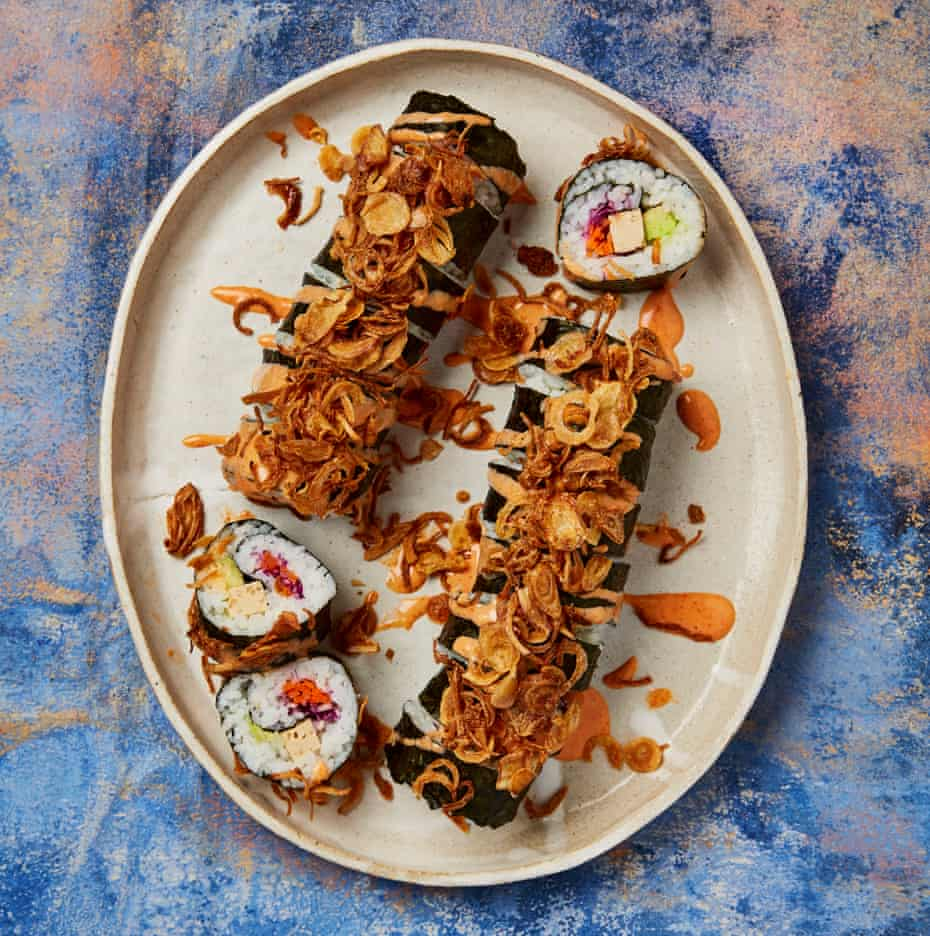
\includegraphics[width=10cm,height=10cm,keepaspectratio]{Recipe_Pictures/Tiger_roll_sushi.png}
\end{figure}
\emph{My old boss used to say that England was such a productive country on account of its cold winters. \\ 
And he had a point, because January is when I tackle more interesting things in the kitchen, such as marmalade, bread-baking and sushi, all of which create a sense of reward to counter the dark and short days.\\ 
And just because sushi is more of a “project” doesn’t mean it’s difficult. For this dish, the only thing you need to cook is the rice; the rest – vegetables, tofu, avocado – is a chopping, mixing and assembly job. So, as recipes go, there’s a decent margin for error.\\ 
The “tiger” comes from the stripes painted on top of the maki roll. It is not an authentic Japanese thing (my apologies), but it is fun. If you can find only half-sheets of nori (such as the Yutaka brand), it’s fine, but you’ll end up with eight smaller rolls. A julienne peeler would be helpful for the carrot.}\\\\ 
\textbf{Prep}: 30 min
\textbf{Cook}: 30 min
\textbf{Serves}: 4
\subsection*{Ingredients}
\begin{itemize}
\item 300g sushi rice
\item 3 tbsp rice-wine vinegar 
\item 4 tsp caster sugar 
\item 1$\frac{1}{4}$ tsp fine sea salt 
\item $\frac{1}{4}$ small red cabbage (about 100g), shredded 
\item 1 medium carrot (about 100g), peeled and cut into matchsticks
\item 1 tbsp sriracha
\item 2 tbsp vegan mayonnaise (I like Leon’s)
\item 4 full sheets nori
\item 110g smoked tofu, cut into 1cm-long batons 
\item 1 avocado, peeled and cut into 1cm-long batons
\item 4 tbsp crisp fried shallots (shop-bought)
\end{itemize}

\subsection*{Steps}
\begin{enumerate}
\item Put the rice in a small pan, cover with lukewarm water, then agitate with your hands until the water turns cloudy. Drain and repeat until the water runs clear. Cover with warm water, leave to soak for five minutes, then drain again.
\item Return the rice to the pan and cover with 400ml cold water. Put on the lid, bring to a boil, then turn down the heat to a whisper and cook for 10 minutes. Turn off the heat and leave to steam, with the lid still on, for 10 minutes more.
\item Meanwhile, in a small bowl mix two tablespoons of the vinegar with the sugar and a teaspoon of salt to make the sushi seasoning. Stir this through the cooked rice, then cover again to keep it warm.
\item In a bowl, toss the cabbage and carrot with the last tablespoon of vinegar and half a teaspoon of salt. In a small bowl, mix the sriracha and mayonnaise, and set aside.
\item Lay a sheet of greaseproof paper on a worktop. Put a sheet of nori shiny side down on the paper and spread a quarter of the rice on top, leaving a 2cm gap at the top end – this will make the sushi easier to roll. Put a line of cabbage and carrot on top of the rice at the end nearest to you, then lay a line of tofu and avocado in the middle of the rice. Wet the open end of the nori with a little water and, using the paper for support, roll as tightly as possible away from you to create a sealed roll. Repeat with the remaining nori and filling.
\item Cut each roll into eight, then push them back together again to recreate a single roll. Put on a platter, drizzle over the sriracha mayo, top with crisp shallots and serve.
\end{enumerate}
\newpage

\section{Salted miso brownies (pictured above)}
\begin{figure}
\centering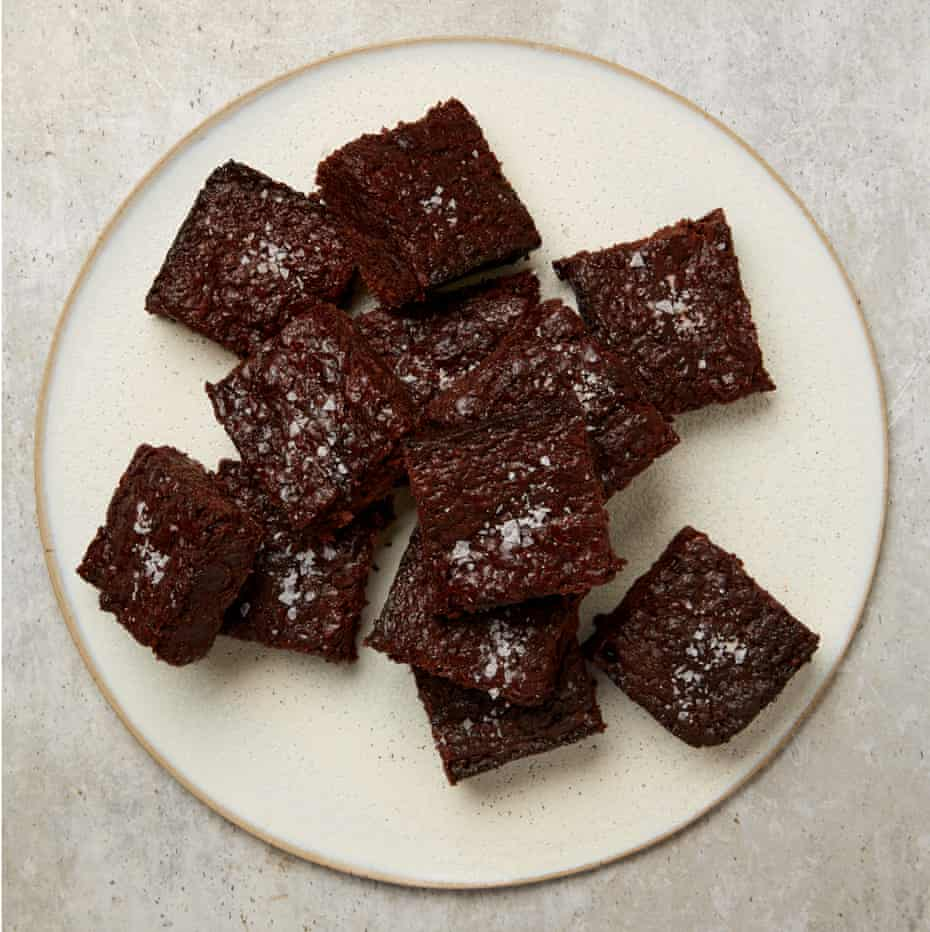
\includegraphics[width=10cm,height=10cm,keepaspectratio]{Recipe_Pictures/Salted_miso_brownies_(pictured_above).png}
\end{figure}
\emph{If I were in charge of brownies and their taxonomy, there would be a proper list of categories. The only thing that unifies them really is the chocolate, beyond which they could be cakey, crumbly, chewy, chocolatey or, er, cocoa-ey. This one is my perfect brownie: dense and fudgy, thanks to the chia seeds; and rich, but not sickeningly so, with a salted caramel-like flavour that comes from using white miso and salt together. It makes this brownie incredibly special. And there is no category for that.\\ 
Make sure you use flavourless coconut oil, unless you actually want to add a coconut flavour, and check that the chocolate is suitable for vegans.}\\\\ 
\textbf{Prep}: 10 min
\textbf{Cook}: 45 min
\textbf{Makes}: 16
\subsection*{Ingredients}
\begin{itemize}
\item 4 $\frac{1}{4}$ tbsp milled chia seeds
\item 150g flavourless coconut oil
\item 250g dark chocolate (85\%), broken into small pieces
\item 420g light brown muscovado sugar
\item 120g plain flour
\item 3 $\frac{1}{4}$ tbsp white miso (shiro miso)
\item 1 tsp flaky sea salt
\end{itemize}

\subsection*{Steps}
\begin{enumerate}
\item Heat the oven to 190c (180C fan)/390F/gas 6, and line a 20cm x 22cm square tin with greaseproof paper. In a small bowl, mix the milled chia seeds with 270ml water and set aside.
\item Put the coconut oil and broken chocolate into a medium-sized saucepan, and set over a low heat. Stir occasionally until melted, then mix in the sugar, flour and miso, and crumble in the salt flakes. Finally, stir in the soaked and bloomed chia seeds, then pour into the lined tin and gently shake to distribute evenly.
\item Bake on the middle shelf of the oven for 45 minutes, then remove. The brownies might still be a bit wobbly in the middle, but they will soon settle down as they cool and be deliciously fudgy. Leave to cool completely, then cut into 16 squares.
\end{enumerate}
\newpage

\section{Tofu akuri (pictured above)}
\begin{figure}
\centering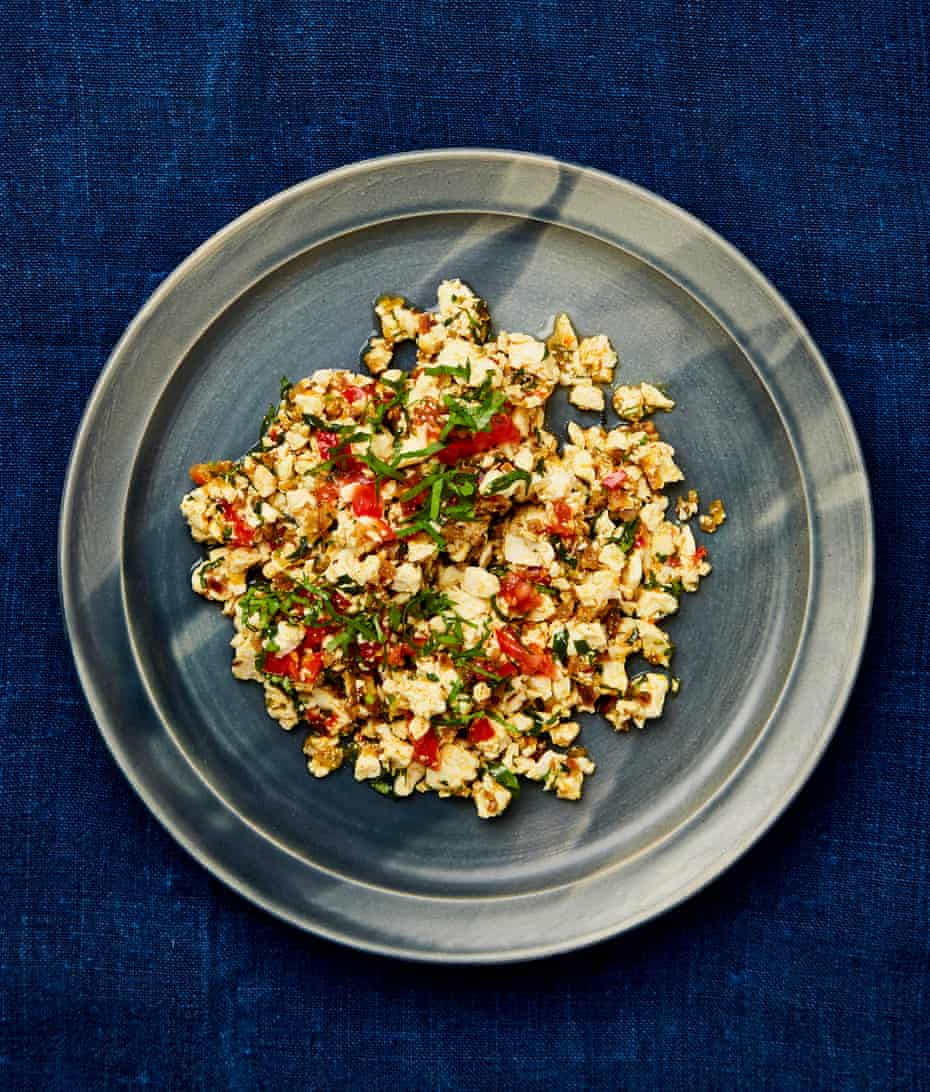
\includegraphics[width=10cm,height=10cm,keepaspectratio]{Recipe_Pictures/Tofu_akuri_(pictured_above).png}
\end{figure}
\emph{}\\\\ 
\subsection*{Ingredients}
\begin{itemize}
\item Prep 10 min
\item Cook 15 min
\item Serves 2
\end{itemize}

\begin{itemize}
\item 500g silken tofu
\item $\frac{1}{4}$ tsp cumin seeds 
\item 2 tbsp rapeseed oil
\item 1 large red onion, peeled and very finely chopped 
\item 1 green finger chilli, very finely chopped 
\item 1 garlic clove, peeled and grated 
\item 1cm piece fresh ginger, peeled and grated 
\item 1 medium sweet vine tomato, finely chopped 
\item 2 tbsp coriander leaves and stalks, finely chopped 
\item $\frac{1}{4}$ tsp ground turmeric
\item $\frac{1}{4}$ tsp salt
\item 4 slices bread, toasted
\end{itemize}

\begin{itemize}
\item Silken, or “soft”, tofu can be found in most big supermarkets or south-east Asian food stores. Serve this on toast with ketchup and a pot of fresh chai.
\end{itemize}

\subsection*{Steps}
\begin{enumerate}
\item Line a sieve with kitchen paper or a clean cloth, then gently place the tofu in the sieve and leave to drain over a bowl for at least 10 minutes.
\item Meanwhile, put the cumin in a mortar and crush to a coarse powder. Heat the oil in a nonstick frying pan and, once hot, stir-fry the cumin for a minute, until you can smell it around the kitchen, then add the onion and fry for eight minutes, until soft, sweet and browning. Add the chilli, garlic and ginger, fry for two minutes, then stir in the tomato, coriander, turmeric and salt.
\item With clean hands, crush the tofu between your fingers into the pan (or mash it in with a potato masher) and cook for a few minutes more, until it’s piping hot and well mixed with the other ingredients. Pile on to the toast and serve immediately.
\end{enumerate}
\newpage

\section{Roast red cabbage and tamarind rasam (pictured above)}
\begin{figure}
\centering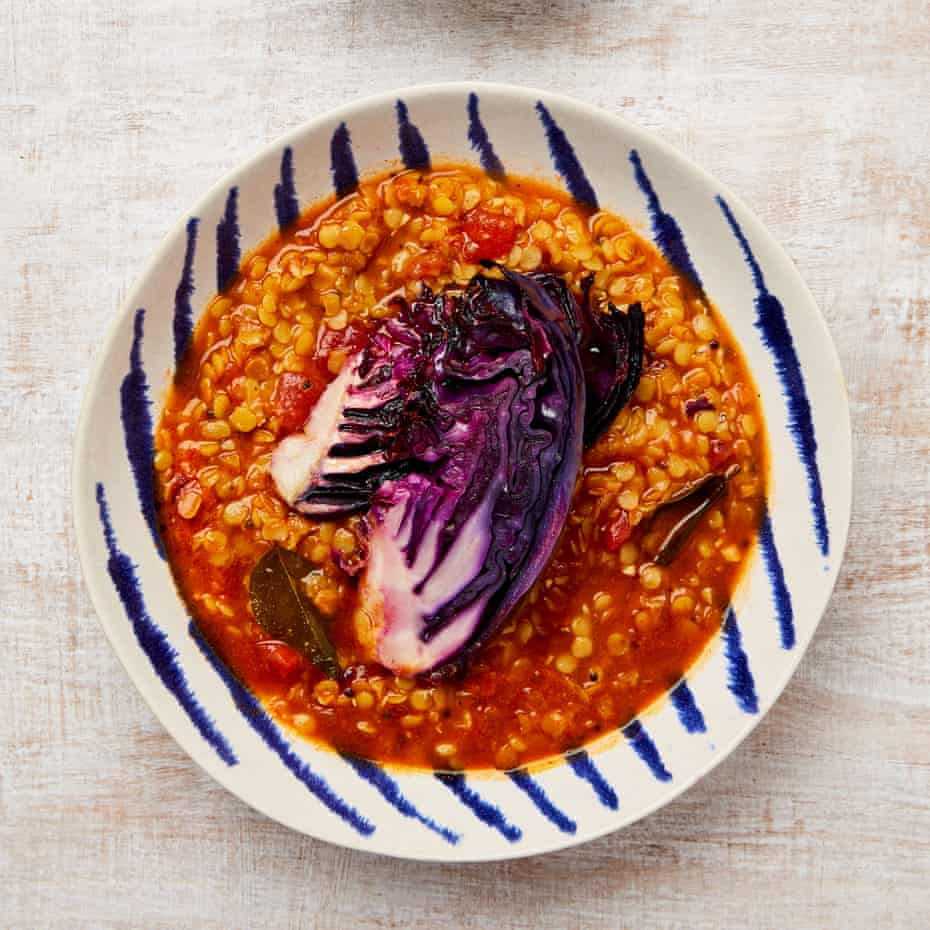
\includegraphics[width=10cm,height=10cm,keepaspectratio]{Recipe_Pictures/Roast_red_cabbage_and_tamarind_rasam_(pictured_above).png}
\end{figure}
\emph{There are dals to comfort and dals to revive. Rasam is a reviver, the kind of thing I want to eat when I’m feeling sluggish. It’s thinner than your average dal, brothy and buzzing with spices, with a defined, sour edge. Here, I serve it with my current addiction, roast red cabbage, whose leaves sweeten, soften and char in the heat of the oven. It’s perfect on its own for a light meal, or with rice for something more substantial.\\ 
Rasam is a hot and sour south Indian soup, sometimes with lentils added. Tamarind and cabbage make good partners.}\\\\ 
\textbf{Prep}: 10 min
\textbf{Cook}: 1 hr
\textbf{Serves}: 4
\subsection*{Ingredients}
\begin{itemize}
\item 1 red cabbage, quartered
\item Rapeseed oil
\item Salt
\item 6 tsp tamarind paste
\item 1 $\frac{1}{4}$ tsp cumin seeds
\item 1 $\frac{1}{4}$ tsp coriander seeds
\item 10 curry leaves
\item 1 $\frac{1}{4}$ tsp black mustard seeds
\item 1 tsp kashmiri chilli powder
\item $\frac{1}{4}$ tsp ground black pepper
\item 5 garlic cloves, peeled and minced
\item 400g tin chopped tomatoes
\item 250g split red lentils
\end{itemize}

\subsection*{Steps}
\begin{enumerate}
\item Heat the oven to 200C (180C fan)/390F/gas 6. Put the quartered cabbage on a lined roasting tray, drizzle with oil, sprinkle with a pinch or two of salt, and roast for 35 minutes.
\item While the cabbage is cooking, make a tamarind dressing. In a small bowl, mix two teaspoons each of tamarind paste and water with a teaspoon of rapeseed oil.
\item When the cabbage is tender to the core and starting to crisp and burn at the edges, remove and brush the cut sides generously with the dressing. Return to the oven for 10 minutes, then set aside.
\item To make the rasam, coarsely grind the cumin and coriander seeds in a mortar. Heat two tablespoons of oil in a large saucepan over a medium heat and, when hot, add the curry leaves, let them crackle for 10 seconds, then add the mustard seeds and let them do the same. Add the ground spices, toast in the hot oil for 30 seconds, then add the garlic and stir-fry until it’s sticky and golden – around three minutes.
\item Now add the tinned tomatoes and all their juices, breaking up any lumps with the back of a spoon. Bring to a simmer, then add the lentils and 1.3 litres water, bring up to a boil and turn down the heat to a gentle simmer. Cook for 30 minutes, stirring occasionally to make sure the lentils don’t stick to the bottom of the pan. Once cooked, add a teaspoon and a quarter of salt and the remaining four teaspoons of tamarind paste, and simmer for a minute more. The texture of the rasam should be somewhere between a soup and a dal.
\item Cut each cabbage quarter into two or three slices. Ladle the rasam into shallow bowls, place a couple of slices of cabbage on top and serve with rice or bread, if you like.
\end{enumerate}
\newpage

\section{Ben ben noodles}
\begin{figure}
\centering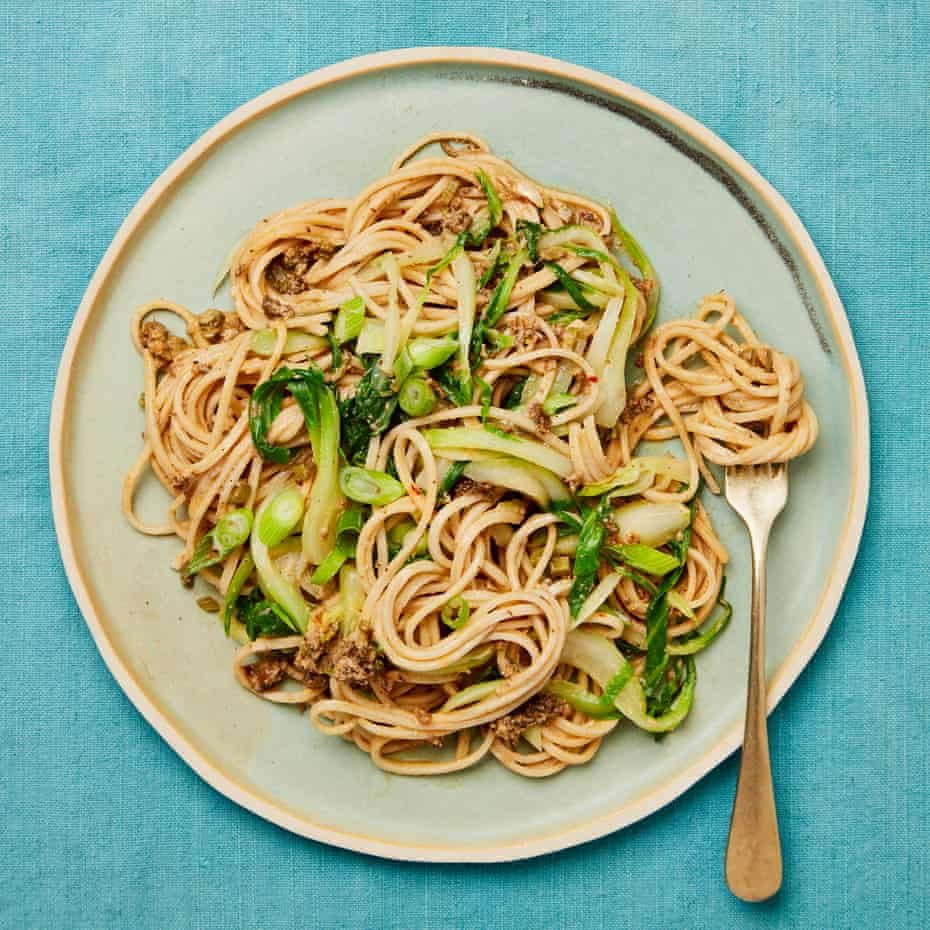
\includegraphics[width=10cm,height=10cm,keepaspectratio]{Recipe_Pictures/Ben_ben_noodles.png}
\end{figure}
\emph{It burst my bubble when I found out that dan dan noodles, the famous Sichuan dish, was not named after two men called Dan, but after the type of pole used by street sellers to carry their baskets of noodles and sauce to sell to passersby. In this instance, however, the name ben ben refers to my friend, the great cook Ben Benton, on whose recipe this is based. Here, shiitake mushrooms rub alongside tahini and roast chilli oil to make an astoundingly good sauce that’s hot enough to put hairs on your chest.\\ 
There are a few ingredients here that you might need to pop to a Chinese food shop for, such as the Shaoxing wine, Chianking vinegar and chilli oil (Lee Kum Kee does a great one), although some are also available in larger supermarkets and online. If you can’t get hold of the wine, use dry sherry, and swap the Chianking for white-wine vinegar; you could even make your own chilli oil, too.}\\\\ 
\textbf{Prep}: 15 min
\textbf{Cook}: 25 min
\textbf{Serves}: 2
\subsection*{Ingredients}
\begin{itemize}
\item 250g shiitake mushrooms
\item 1 tsp Sichuan peppercorns
\item 1 tbsp oil
\item 40g gherkins or pickled cucumber, finely chopped
\item 2 spring onions, sliced on the diagonal, whites and greens separated
\item 1 tbsp Shaoxing rice wine (or dry sherry)
\item 2 tsp light soy sauce
\item 200g wholewheat noodles
\item 200g baby pak choi or similar greens, shredded
\end{itemize}

\begin{itemize}
\item For the sauce
\item 3 tbsp tahini
\item 3 tbsp light soy sauce
\item 1 tbsp Sichuan roasted chilli oil, with sediment, plus an extra drizzle to finish
\item 1 tbsp Chianking black-rice vinegar
\end{itemize}

\subsection*{Steps}
\begin{enumerate}
\item Blitz the mushrooms in a food processor to lentil-size pieces – be careful they don’t turn to soup. 
\item Put the peppercorns in a dry frying pan on a low heat and toast until fragrant – about four minutes, but be vigilant because they burn easily – then remove and grind. In the same pan, heat the oil on a high flame. When hot, fry the chopped mushrooms, pressing them into a single layer to maximise contact with the pan, for eight to 10 minutes, until dark brown and beginning to crisp up. Add the gherkins, spring onion whites and the ground Sichuan pepper, fry for two minutes, then add the wine and soy, and cook for two minutes more, until dry and crunchy.
\item Mix all the sauce ingredients in a small bowl. It will look a little split at first, but just keep mixing until it comes together.
\item Cook the noodles in boiling water according to the packet instructions, stirring to separate them, and add the pak choi for the final two minutes. Just before the noodles are done, remove a mugful of the cooking water, then drain and put the noodles and greens in a large bowl. Mix in the sauce, the mushrooms and the reserved cooking water, tablespoon by tablespoon (I needed six), until the noodles are nice and saucy.
\item Divide between two plates, sprinkle with the spring onion greens and a drizzle more oil, and serve.
\end{enumerate}
\newpage

\section{Most popular}
\begin{figure}
\centering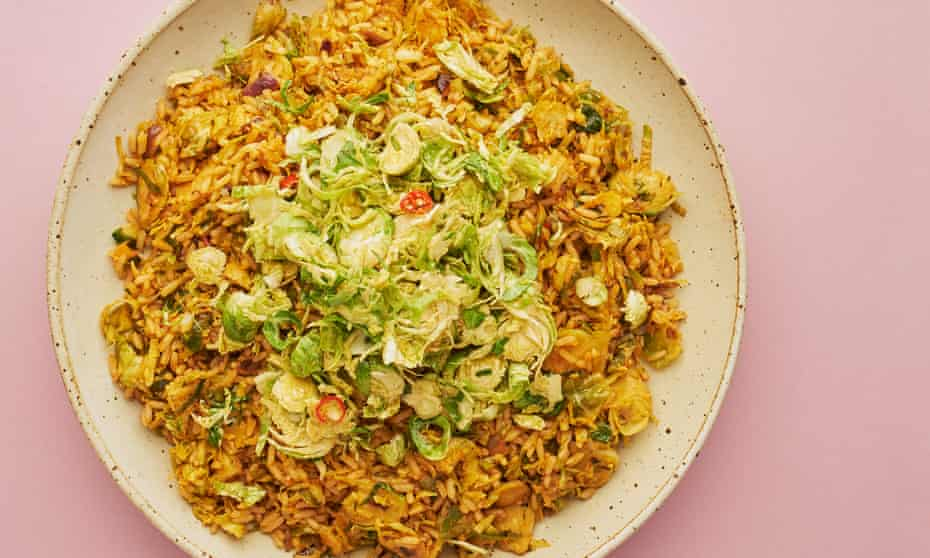
\includegraphics[width=10cm,height=10cm,keepaspectratio]{Recipe_Pictures/Most_popular.png}
\end{figure}
\emph{Sometimes, all you really want is something with that sort of filthy and delicious taste that I used to think only a good takeaway could provide – until I accidentally recreated it while writing this recipe for Malaysian nasi goreng. It’s fried rice, but not as you know it: smothered in unami-ific sauces, and topped with shredded, marinated sprouts for crunch and zing. All the joy of a takeaway, but without the wait or delivery charge.\\ 
Kecap manis is a sweet soy sauce that can be found in larger supermarkets, online and in south-east Asian food shops. I cut the sprouts by hand, but you could use the slicing attachment on a food processor.}\\\\ 
\textbf{Prep}: 10 min
\textbf{Cook}: 30 min
\textbf{Serves}: 4
\subsection*{Ingredients}
\begin{itemize}
\item 350g jasmine rice
\item 3 tbsp rapeseed oil 
\item 1 red onion, peeled and chopped 
\item 4 garlic cloves, peeled and crushed 
\item 3 bird’s eye chillies, very finely chopped (deseeded, if you prefer less heat)
\item 750g brussels sprouts, very finely sliced 
\item 2 tbsp tomato puree
\item 2 tbsp kecap manis
\item 1 $\frac{1}{4}$ tsp salt
\item 2 tbsp soy sauce 
\item 1 tbsp white-wine vinegar 
\item 2 tbsp toasted sesame oil 
\item 1 tsp sugar
\end{itemize}

\subsection*{Steps}
\begin{enumerate}
\item Put the rice in a sieve and wash under the cold tap until the water runs clear. Tip the rice into a pan, add 500ml fresh cold water and bring to a boil. Turn down the heat to a whisper, cover the pan and leave to cook for 15 minutes. Turn off the heat and leave with the lid still on, to steam through.
\item To cook the nasi goreng base, heat the rapeseed oil in a large frying pan on a medium flame and, when hot, fry the onion, stirring, for five minutes. Add the garlic and two-thirds of the chopped chillies, cook for two minutes more, then add all but two large handfuls (or about 150g) of the sprouts. Fry for eight minutes, leaving them undisturbed for a couple of minutes at a time, so they get some colour on them. Then stir in the tomato puree, kecap manis, salt and a tablespoon each of soy sauce and vinegar. Cook for another five minutes, then take off the heat.
\item To make the marinated sprouts, put the remaining raw sliced sprouts in a bowl with the soy sauce, white-wine vinegar, toasted sesame oil, sugar and the remaining chopped chilli. Mix very well and set aside.
\item To finish the nasi goreng, put the sprout and onion pan on a medium heat and gently scoop in the steamed rice, folding it in until well mixed. Heat through, stirring gently, for five minutes, until the rice is nice and hot, and season to taste. Transfer to a big platter, scatter the marinated sprouts over the top and serve.
\item Photography: Rob White. Food stylist: Amy Stephenson.
\end{enumerate}
\newpage

\section{Sweet potato and aubergine massaman curry}
\begin{figure}
\centering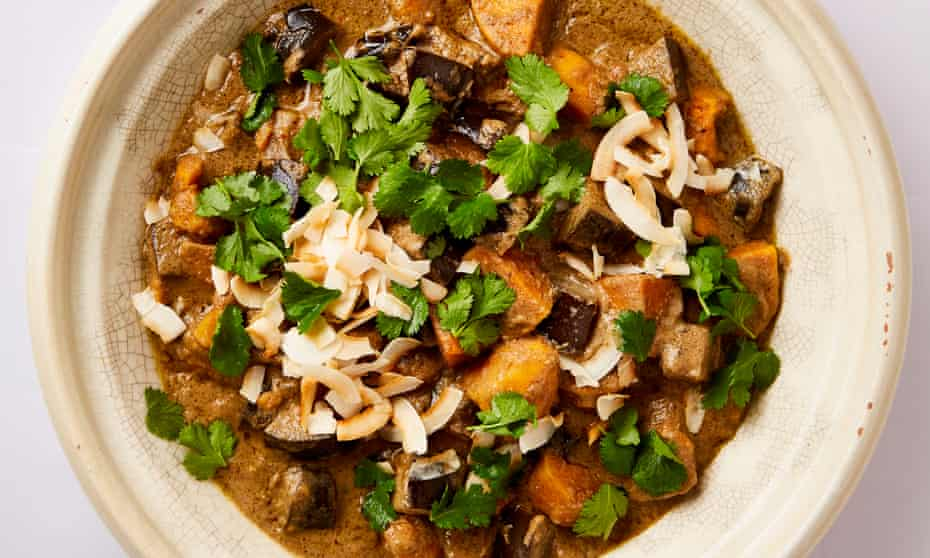
\includegraphics[width=10cm,height=10cm,keepaspectratio]{Recipe_Pictures/Sweet_potato_and_aubergine_massaman_curry.png}
\end{figure}
\emph{‘Something from the cupboard” was a regular meal when I was growing up. Our family home was in the countryside and a good distance from the shops, so going out in January to buy something fresh meant de-icing our old Nissan Bluebird that was so full of holes, eye-stinging wind would whip around our necks and freeze our fingers blue. The thought of something from the cupboard, then, was a source of great comfort, and a foil to our laziness, because it meant we didn’t need to leave the house.\\ 
Naturally, we spent a lot of time with our noses in the kitchen drawers, wondering how best to use tins of this and pots of spices, alongside stalwarts of the vegetable basket, and turn them into meals. Most of the time, this resulted in the same old things: spinach and sweetcorn saag (makai palak), plum tomato and chickpea noodle curry (sev tamatar) and dal dhokli (chickpea pasta poached in dal).\\ 
But now that there is easy access to a more varied and global pantry, I tend to push the boat out and cook my way around south-east Asia on a regular basis: pad thai, laksa, penang curry and massaman curry share many ingredients in common – coconut milk, nuts, tamarind and galangal paste – as well as spices that keep for months, if not years. All are also forgiving enough to absorb most of our seasonal produce, while many of the base pastes can be made in a blender without a significant dent to flavour.\\ 
Today’s recipe is just such a dish. According to Thai food guru David Thompson, massaman curry has “all the hallmarks of southern Muslim food – rich with coconut cream and redolent of spices”. There are many variations, but it’s usually sweet, sour with tamarind and made using spices, peanuts and coconut; it also often features a starchy vegetable such as potato or sweet potato. Ordinarily complex to make, I’ve taken liberties by using as many store-cupboard ingredients as possible.\\ 
Feel free to play around with the vegetable element: potatoes, broccoli, carrots and radishes would all be at home here. Serves four.}\\\\ 
\subsection*{Ingredients}
\begin{itemize}
\item For the paste
\item 5 red bird’s-eye chillies
\item 4 shallots, peeled and roughly chopped
\item 2 lemongrass stalks, tough outer leaves removed, then roughly chopped
\item 50g bunch coriander, leaves picked and set aside, stalks roughly chopped
\item 100g (4$\frac{1}{4}$ tbsp) smooth peanut butter 
\item 1$\frac{1}{4}$ tsp ground cumin
\item $\frac{3}{4}$ tsp ground cinnamon
\item $\frac{1}{4}$ tsp ground cloves
\item 1$\frac{1}{4}$ tbsp galangal paste
\item 1$\frac{1}{4}$ tbsp tamarind paste
\item 2$\frac{1}{4}$ tsp sugar 
\item 1$\frac{1}{4}$ tsp salt
\end{itemize}

\begin{itemize}
\item For the curry 
\item 2 x 400ml tins coconut milk
\item 400g aubergine, cut into 2cm x 2cm chunks
\item 800g sweet potatoes, peeled and cut into 3cm x 3cm chunks
\item 1 handful dried coconut slices, to garnish 
\end{itemize}

\subsection*{Steps}
\begin{enumerate}
\item Put all the ingredients for the paste in a blender, add 100ml water and blitz to a paste.
\item Put a large pan for which you have a lid on a medium heat and, once hot, fry the paste, stirring constantly, for five minutes, until dark and glossy; take care it doesn’t catch and burn. Add the coconut milk little by little, stirring it into the paste as you go, then throw in the aubergine and bring the lot up to a bubble. Add the sweet potato, cover the pot, turn down the heat to a whisper and leave to cook for 20 minutes, until the aubergine has collapsed and the sweet potato is very tender.
\item While the curry is cooking, toast the coconut slices. Put a small frying pan on a medium flame and, once hot, toast the coconut for a couple of minutes, until golden brown on both sides, then tip out on to a plate.
\item To serve, transfer the curry to a serving bowl, scatter the coriander leaves and coconut slices on top, and serve with plain rice.
\end{enumerate}
\newpage

\section{Aloo paratha with quick lemon pickle}
\begin{figure}
\centering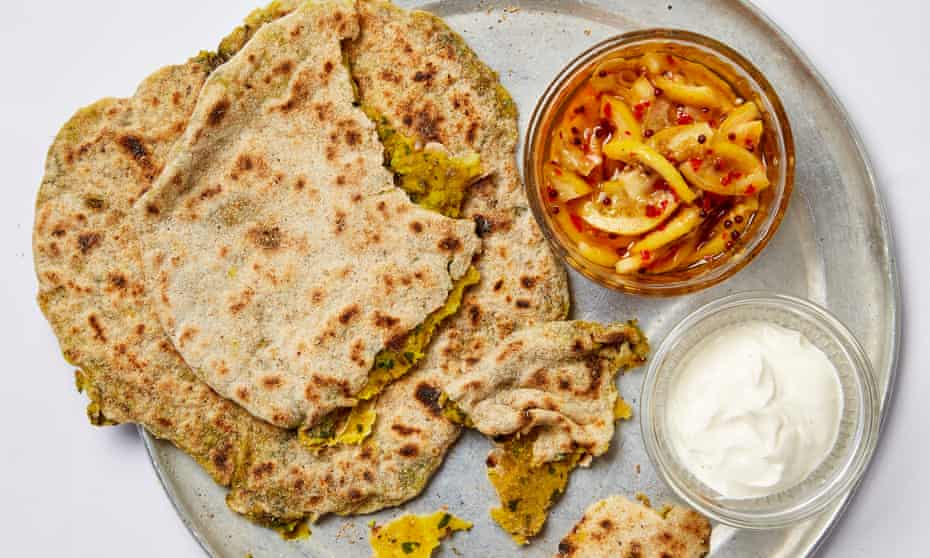
\includegraphics[width=10cm,height=10cm,keepaspectratio]{Recipe_Pictures/Aloo_paratha_with_quick_lemon_pickle.png}
\end{figure}
\emph{Beige food has had a difficult few years: it has been all but cast out of media appearances (with the exception of sourdough). We have become so obsessed with what our food looks like that we sometimes forget that, actually, appearances aren’t everything. What really matters is how food tastes, and how much pleasure it gives us – and that includes ugly and brown food.\\ 
Aloo paratha, one of my all-time favourite dishes, will never win a beauty contest. In India, it is the breakfast of champions, but I’ll happily make room for it at any time of day. It might not get 1,000 likes on social media, but it’s proof that beige can also be brilliant.\\ 
If you can’t find chapati flour, use a mix of wholewheat and white, though you may need a bit more water. And don’t worry if your paratha is not completely round: practice makes perfect. (Incidentally, you can freeze leftover parathas: lay a square of greaseproof paper between each one and put them in a sealed container.) Makes eight.}\\\\ 
\subsection*{Ingredients}
\begin{itemize}
\item 2 lemons 
\item Rapeseed oil 
\item $\frac{1}{4}$ tsp black mustard seeds 
\item 1 fat garlic clove, peeled and thinly sliced 
\item 1 red chilli, finely chopped (deseeded, if you want less heat) 
\item Salt 
\item 2 medium maris piper potatoes (about 350g), peeled
\item 350g chapati flour 
\item 2cm ginger, grated 
\item 1 red onion, peeled and very finely diced 
\item 1$\frac{1}{4}$ green finger chillies, very finely chopped (deseeded, if you prefer less heat)
\item 30g fresh coriander, stems and leaves, very finely chopped 
\item $\frac{1}{4}$ tsp turmeric 
\item $\frac{1}{4}$ tsp cumin seeds
\item Non-dairy yoghurt, to serve 
\end{itemize}

\subsection*{Steps}
\begin{enumerate}
\item First make the pickle. Top and tail one lemon, cut it into four, then cut each quarter into very thin slices (use your sharpest knife), removing any pips. Put the slices in a bowl, and juice the other lemon over the top.
\item On a very low flame, heat two tablespoons of oil in a pan for which you have a lid. Add the mustard seeds and garlic, and when the garlic turns pale gold, add the red chilli, lemon slices, lemon juice and half a teaspoon of salt. Stir to mix, cover and leave to cook for five minutes. Remove the lid, cook for five minutes more, until the oil starts to split from the lemons, then take off the heat and leave to cool.
\item Cut the potatoes into quarters and put in a deep saucepan. Cover with cold water, bring to a boil and cook until tender. Drain and leave to cool.
\item Meanwhile, make the dough. Put the flour in a bowl, make a well in the centre and pour in two tablespoons of oil and half a teaspoon of salt. Mix with your hands until it resembles breadcrumbs, then bit by bit work in 220ml hand-hot water, until you have a soft dough. Cover and set aside.
\item Roughly mash the cooled potato, then mix in the ginger, onion, green chilli, coriander, turmeric, cumin and three-quarters of a teaspoon of salt. Combine with your hands, until well mixed, thick and starchy, then taste and adjust the seasoning.
\item Divide the dough into eight and roll each piece into a ball between your palms. Flatten a little, then dip in flour and roll out to 14cm in diameter. Take a golf ball-sized amount of potato mix, roll it into a ball and put in the middle of the paratha. Pull the edges of the dough up around the ball, seal and flatten. Dip in flour and roll out to 14cm in diameter. Repeat with the rest of the dough and filling.
\item Heat a frying pan on a medium flame and, once hot, lay in a paratha and cook for a minute, until brown spots appear on the underside. Flip over, cook for a minute on the other side, then flip twice more, giving both sides a final 30 seconds on the heat (by this time, there should be no doughy bits visible). Transfer to a plate and keep warm while you repeat with the remaining parathas.
\item Serve fresh and hot with the pickle and a dollop of non-dairy yoghurt. 
\end{enumerate}
\newpage

\chapter{February}
\section{Tagliatelle with charred red pepper sauce and salsa verde}
\begin{figure}
\centering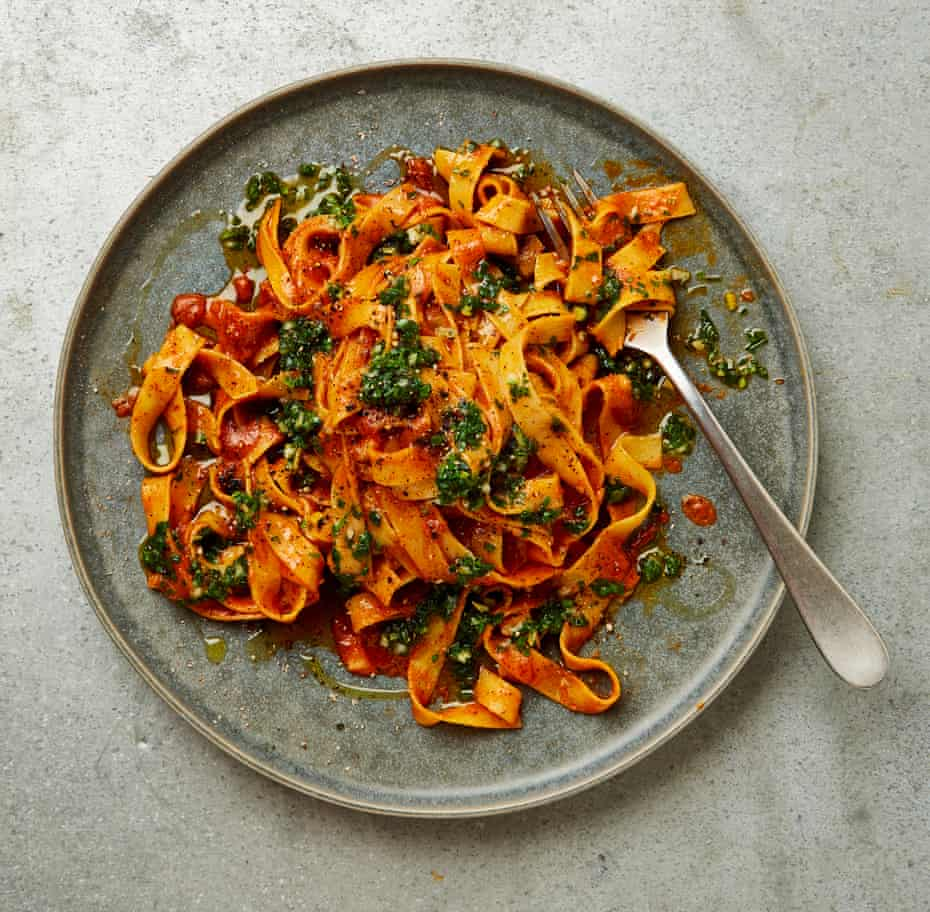
\includegraphics[width=10cm,height=10cm,keepaspectratio]{Recipe_Pictures/Tagliatelle_with_charred_red_pepper_sauce_and_salsa_verde.png}
\end{figure}
\emph{There are lots of uses for this charred red pepper sauce. It’s lovely tossed through pasta, but you could also serve it with jarred butter beans or as a soup, each time with the zingy salsa spooned on top to cut through the richness. If you’re going with the pasta, feel free to be creative with the shape you use; gnocchi, pappardelle or paccheri are all great options. It may not look as if there’s much going on in the ingredients list for the sauce, but, trust me, you’ll want to eat it straight out of the blender with a spoon.\\ 
Don’t skip the dried onion granules: they might seem a bit of an obscure, unnecessary ingredient, but they provide an extra level of concentrated umami and are widely available besides. Ideally, grate the nutmeg yourself, rather than using ready ground, which can be a little bitter.}\\\\ 
\textbf{Prep}: 10 min
\textbf{Cook}: 30 min
\textbf{Serves}: 4
\subsection*{Ingredients}
\begin{itemize}
\item 250g dried tagliatelle (or another pasta)
\end{itemize}

\begin{itemize}
\item For the sauce
\item 340g red romano peppers (ie, 3-4 peppers)
\item 125g plant-based cream, or full-fat tinned coconut milk
\item 25g white miso paste
\item 25g tomato paste 
\item 2 tbsp olive oil 
\item 1 small garlic clove, peeled
\item 1 tsp dried onion granules
\item 1 tsp freshly grated nutmeg (or $\frac{1}{4}$ tsp ground nutmeg), plus extra to serve
\item $\frac{1}{4}$ tsp paprika (not smoked)
\item Salt and black pepper
\end{itemize}

\begin{itemize}
\item For the salsa
\item 10g chives, very finely chopped (about 3$\frac{1}{3}$ tbsp)
\item 5g parsley, very finely chopped (about 1$\frac{1}{4}$ tbsp)
\item 2 thin slices lemon, skin left on, deseeded and very finely chopped
\item 3 tbsp olive oil
\end{itemize}

\subsection*{Steps}
\begin{enumerate}
\item Heat the oven grill to its highest setting. Lay out the peppers on a flat baking tray and grill on the top shelf for about eight minutes, until soft and blackened in patches. Turn and grill for another seven or eight minutes, until the other side is soft and blackened in patches, too – keep an eye on them, though: if your grill is particularly powerful, they may be ready sooner.
\item Remove the pepper stalks, pith and seeds, then put the rest in a blender (there’s no need to peel the peppers). Add all the remaining sauce ingredients, a quarter-teaspoon of fine salt and lots of black pepper (I used about 50 twists of the mill), then blitz smooth. Pour the sauce into a large saute pan and set aside.
\item Put all the ingredients for the salsa verde in a small bowl, add an eighth of a teaspoon of fine salt and some black pepper to taste, mix to combine and set aside.
\item Cook the pasta in salted boiling water as per the packet instructions. until al dente, then drain, reserving 325ml of the cooking water.
\item Put the saute pan with the sauce on a medium-high heat, then add the reserved pasta water and bring to a simmer. Add the drained tagliatelle and toss over the heat for 90 seconds to two minutes, just until the pasta and sauce have emulsified.
\item Add more salt to taste, if need be, then divide between four plates and drizzle over some of the salsa. Finish with a grating of nutmeg, some black pepper and more olive oil, and serve.
\end{enumerate}
\newpage

\section{Oyster mushrooms with tomato chipotle butter sauce and creamy polenta}
\begin{figure}
\centering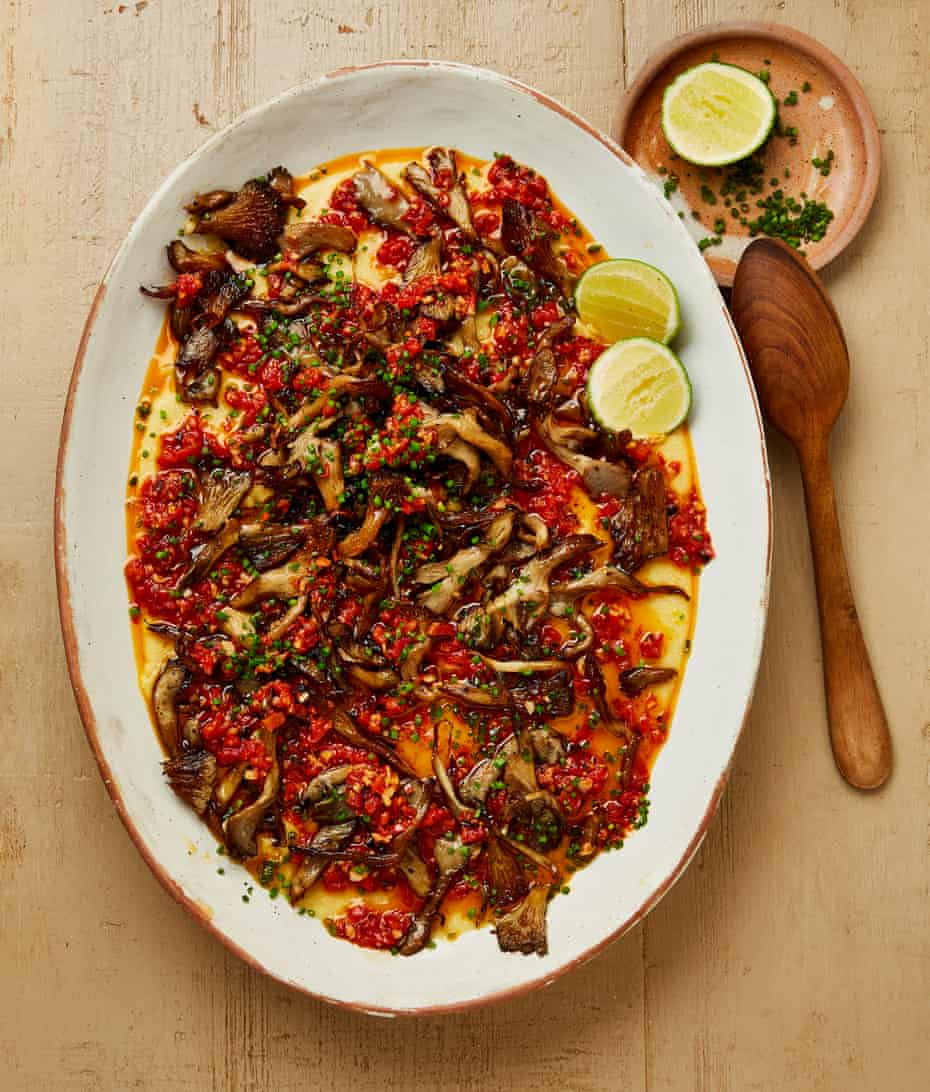
\includegraphics[width=10cm,height=10cm,keepaspectratio]{Recipe_Pictures/Oyster_mushrooms_with_tomato_chipotle_butter_sauce_and_creamy_polenta.png}
\end{figure}
\emph{Oyster mushrooms have the power to turn into incredibly crisp, meaty versions of themselves when fried or roasted. I love them, but I’m aware that many people don’t, and even more aware that mushrooms are all too often used as a substitute for meat. With that in mind, I urge you not to skip over this recipe if you don’t like mushrooms: roasted aubergine cubes are a great alternative, and go just as well with the tomato and chipotle butter sauce and creamy polenta.\\ 
Both the fresh chilli and the chipotle chilli flakes are optional, so omit them, or just use less, if you prefer. For the aubergine version of this dish, cut 500g aubergines into 3cm cubes, toss with four tablespoons of oil and a teaspoon of salt, spread out on a flat, lined oven tray and roast in a 230C (210C fan)/450F/gas 8 oven for half an hour, stirring once halfway, until deeply golden brown.}\\\\ 
\textbf{Prep}: 10 min
\textbf{Cook}: 40 min
\textbf{Serves}: 4
\subsection*{Ingredients}
\begin{itemize}
\item For the mushrooms
\item 500g oyster mushrooms, torn in half or, if large, in quarters
\item 3 tbsp olive oil
\item Fine salt and black pepper
\end{itemize}

\begin{itemize}
\item For the tomato chipotle sauce
\item 4 tbsp olive oil
\item 30g plant-based butter
\item 4 garlic cloves, peeled and very finely chopped 
\item 1 mild red chilli, deseeded and very finely chopped (or less, to taste)
\item 150g sweet, ripe cherry tomatoes (such as datterini), very finely chopped 
\item 1 tsp tomato puree
\item $\frac{3}{4}$ tsp smoked paprika
\item $\frac{1}{4}$ tsp chipotle chilli flakes (or less, to taste)
\end{itemize}

\begin{itemize}
\item For the polenta
\item 200ml plant-based single cream or full-fat tinned coconut milk (at least 70\% coconut extract)
\item 100g quick-cook polenta
\item 60g white miso paste
\item 1 tbsp olive oil
\item 1 tsp dried onion granules
\end{itemize}

\begin{itemize}
\item To serve
\item 1$\frac{3}{4}$ tbsp (5g) finely chopped chives
\item 1 lime, cut into wedges
\end{itemize}

\subsection*{Steps}
\begin{enumerate}
\item Heat the oven to 210C (190C fan)/410F/gas 6$\frac{1}{4}$. Line a large, flat oven tray with greaseproof paper. Top with the torn mushrooms, oil, salt and plenty of pepper, toss to coat, then spread out evenly and roast for 20 minutes. Stir, roast for another five to 10 minutes, until crisp and golden brown, then remove and set aside.
\item Meanwhile, make the sauce. Put the oil and butter in a medium, nonstick frying pan on a low heat. Once the butter has melted, add the garlic, chilli and half a teaspoon of fine salt and fry very gently, stirring often, for three to four minutes, until the garlic is soft and golden (you don’t want it to brown or go crisp, so keep the heat very low). Take off the heat and immediately stir in the tomatoes, tomato paste, paprika, chipotle and plenty of black pepper, then set aside.
\item Put all the ingredients for the polenta in a medium saucepan, add 350ml water and whisk to combine. Put on a medium heat and cook, whisking continuously, for about six minutes, until smooth and thickened (if at any point the polenta starts to spit, turn the heat down).
\item Spoon the polenta on to a platter or four individual plates, then spoon over the sauce, followed by the mushrooms. Drizzle over some more oil, scatter the chives on top and serve with the lime wedges alongside.
\end{enumerate}
\newpage

\section{Sticky rice-stuffed aubergines}
\begin{figure}
\centering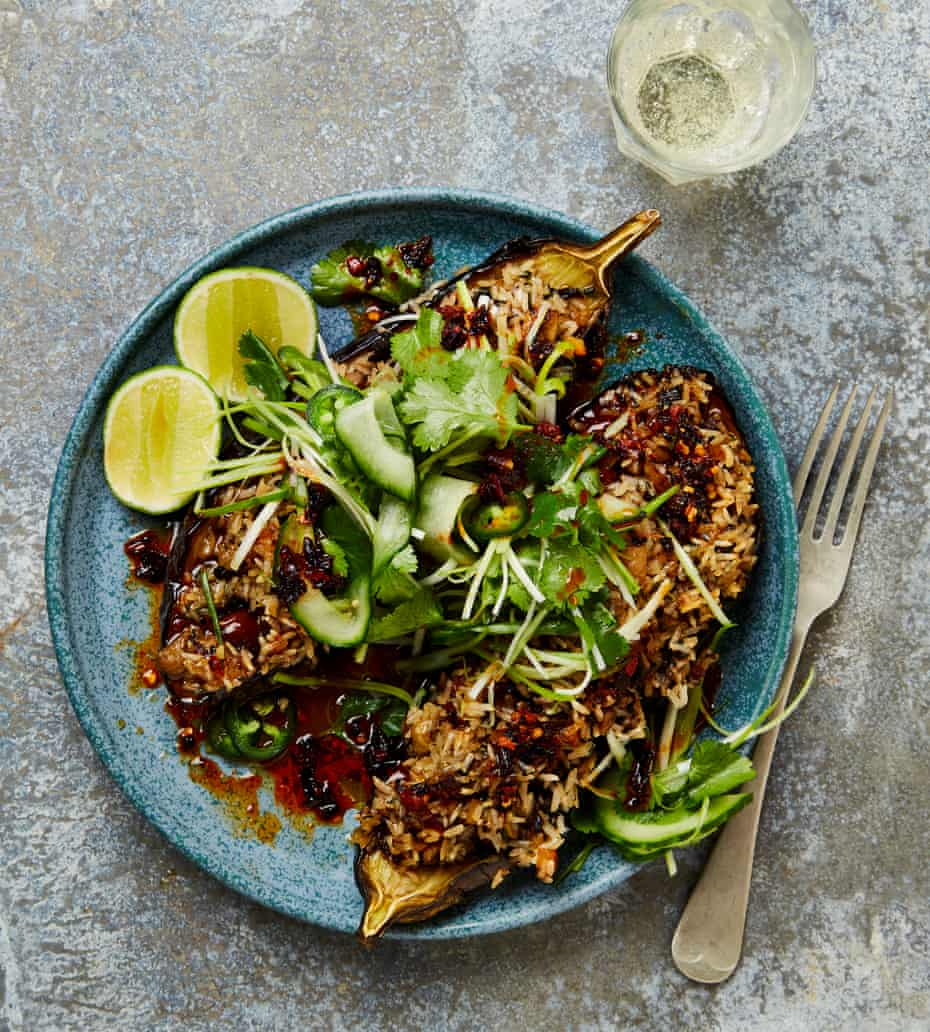
\includegraphics[width=10cm,height=10cm,keepaspectratio]{Recipe_Pictures/Sticky_rice-stuffed_aubergines.png}
\end{figure}
\emph{Today’s recipe is loosely inspired by lo mai gai, a Cantonese dish of sticky rice with chicken that also often features dried mushrooms, Chinese sausage and dried prawns. In this version, aubergines are halved and roasted, then the flesh is added to a sweet, savoury and slightly spicy mix of sticky rice, dried mushrooms, chestnuts, ginger and chives. The rice is then stuffed back into aubergine skins and baked until it’s deliciously sticky on the inside and crisp on the outside. Incredibly flavourful and, dare I say, meaty, this dish is well worth the effort, I promise.\\ 
I use Thai Taste sticky rice, which needs only two hours of pre-soaking in order to cook through inside the aubergines. If you have another brand, check the packet, because the rice may well need an overnight soak.}\\\\ 
\textbf{Prep}: 15 min
\textbf{Cook}: 2 hr
\textbf{Soak}: 2 hr+
\textbf{Serves}: 4
\subsection*{Ingredients}
\begin{itemize}
\item 4 medium aubergines (about 250g each), cut in half lengthways
\item 10 tbsp olive oil
\item Fine salt and black pepper
\item Chiu chow oil, or crispy chilli oil, to finish
\item 1 lime, cut into wedges, to serve
\end{itemize}

\begin{itemize}
\item For the rice mix
\item 400g Thai sticky rice (aka glutinous rice) – I use Thai Taste
\item 30g dried wild mushrooms
\item 120g ready-cooked and peeled chestnuts, finely chopped
\item 15g fresh ginger, peeled and finely grated
\item 20g chives, finely chopped
\item 2 garlic cloves, peeled and finely grated or crushed
\item 3$\frac{1}{4}$ tbsp maple syrup
\item 4 tbsp soy sauce
\item 20g sriracha, or less, to taste
\end{itemize}

\begin{itemize}
\item For the spring onion salad
\item 20g spring onions, julienned
\item $\frac{1}{4}$ cucumber, halved lengthways, deseeded and finely sliced at an angle
\item 10g coriander leaves
\item 1 fresh jalapeño chilli, sliced into thin rounds (optional)
\item 1 tbsp lime juice
\end{itemize}

\subsection*{Steps}
\begin{enumerate}
\item Heat the oven to 240C (220C fan)/475F/gas 9. Put the rice in a bowl, add cold water to cover, then leave to soak for two hours, or overnight (see recipe introduction).
\item Cut cross-hatches into the flesh of each aubergine half, cutting about three-quarters of the way down into the flesh, taking care not to puncture the skin and leaving a $\frac{1}{4}$cm border around the edges. Lay the aubergines cut side up on a large, flat baking tray.
\item In a small bowl, mix four tablespoons of the olive oil and a teaspoon of fine salt, then rub this mix all over the cut sides of the aubergines. Bake in the hot oven for 35-40 minutes, turning the tray once halfway, until very well browned, then remove and leave to cool.
\item While the aubergines are baking, put the dried mushrooms in a small bowl, cover with just-boiled water and leave to soak for 15 minutes.
\item Turn down the oven to 210C (190C fan)/410F/gas 6$\frac{1}{4}$. In a medium bowl, combine the chestnuts, ginger, chives, garlic, remaining six tablespoons of olive oil, maple syrup, soy sauce, sriracha, a teaspoon of fine salt and lots of pepper – I used about 30 twists of the grinder. Drain and finely chop the mushrooms, then add them to the chestnut bowl. Scoop the flesh from the cooked aubergines into the bowl, taking care not to tear the skins. 
\item Drain the soaked rice, add that to the bowl, too, then mix well to combine.
\item Lay the scooped-out aubergine skins in a 33cm x 26cm high-sided baking tray. Fill each half with an eighth of the rice mix, then drizzle a tablespoon of water evenly over each one. Drizzle with a little more olive oil, cover very tightly with foil, so no steam can escape, and bake for an hour. Remove the foil, bake uncovered for five minutes more, then remove and leave to rest and cool for 10 minutes.
\item Meanwhile, make the salad: in a small bowl, mix the spring onions, cucumber, coriander, jalapeño, lime juice and a good pinch of salt. Transfer the aubergines to a platter or individual plates, top with some salad, then drizzle over some chilli oil to taste and serve with lime wedges on the side.
\end{enumerate}
\newpage

\section{Creamy saffron orzo with roast butternut and scotch bonnet}
\begin{figure}
\centering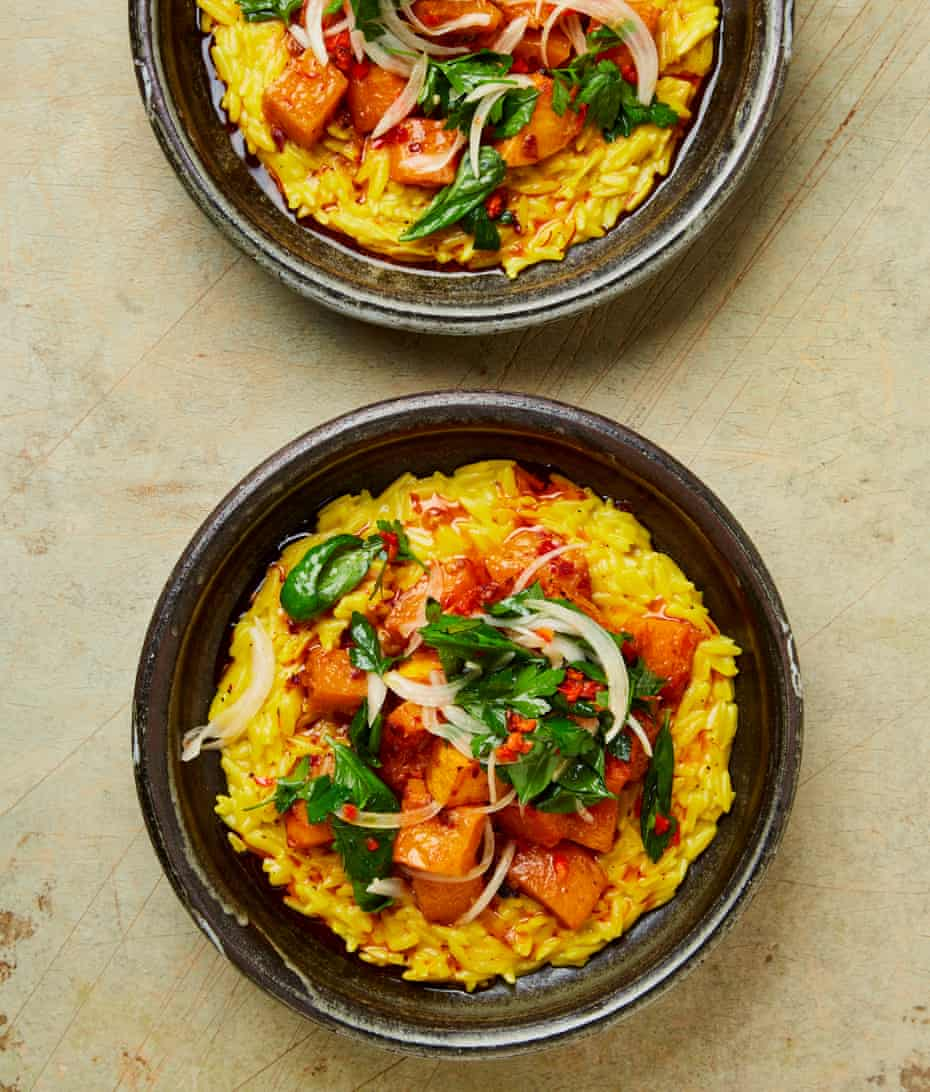
\includegraphics[width=10cm,height=10cm,keepaspectratio]{Recipe_Pictures/Creamy_saffron_orzo_with_roast_butternut_and_scotch_bonnet.png}
\end{figure}
\emph{When I was asked to look after this column while Meera Sodha takes a well-deserved break, I was both nervous (those are some big metaphorical shoes to fill) and excited, but I won’t pretend I wasn’t also slightly apprehensive of the fact that this is a vegan column. Not because I don’t love vegetables (I do!), but because I didn’t want to come across as disingenuous (let it be known that I’m very much an omnivore) and also because the idea of being limited by the ingredients I could use worried me. I’m happy to report, however, that this has been a welcome challenge and that, in the right circumstances, limitations can push the boundaries of creativity.\\ 
Scotch bonnet chillies are very hot. If you prefer less heat, use one or two mild red chillies instead, or leave out the chilli altogether; there’s plenty of flavour coming from other directions here. The coconut milk is all but undetectable – it just helps create a creamy base for the sweet squash.}\\\\ 
\textbf{Prep}: 10 min
\textbf{Cook}: 40 min
\textbf{Serves}: 4
\subsection*{Ingredients}
\begin{itemize}
\item For the butternut
\item 1 large butternut squash (1.2kg), peeled, halved, deseeded and flesh cut into 2$\frac{1}{4}$cm cubes (800g net weight)
\item 1 scotch bonnet chilli (optional)
\item 1 mild red chilli (or 2 if not using the scotch bonnet; optional)
\item 50g plant butter, cut into cubes
\item 4 tbsp olive oil
\item 40g white miso paste 
\item 2 tbsp maple syrup
\item 2 tsp rose harissa 
\item 2 cinnamon sticks, or $\frac{1}{8}$ tsp ground cinnamon
\end{itemize}

\begin{itemize}
\item For the orzo
\item 250g dried orzo
\item 300ml full-fat tinned coconut milk (at least 70\% coconut extract)
\item Fine salt and black pepper
\item $\frac{1}{4}$ tsp saffron threads
\item Freshly grated nutmeg
\end{itemize}

\begin{itemize}
\item To serve
\item 5g fresh parsley leaves
\item 5g fresh basil leaves
\item $\frac{1}{4}$ small white onion, very thinly sliced
\item 2 tsp olive oil
\item 1 lemon, halved
\end{itemize}

\subsection*{Steps}
\begin{enumerate}
\item Heat the oven to 240C (220C fan)/475F/gas 9. Put all the butternut ingredients and a half-teaspoon of fine salt in a 32cm x 36cm high-sided baking tray and toss to coat. Cover tightly with foil, bake for 15 minutes, then remove the foil and bake for another 18 minutes, stirring once halfway, until soft, golden brown and bubbling. Discard the cinnamon sticks, if using. Lift out the chillies, if using, then deseed, finely chop and set aside.
\item While the butternut is roasting, put the orzo in a bowl, pour over just-boiled water to cover and leave to soak for 10 minutes. Drain, then rinse under cold running water to separate the grains.
\item When the butternut has about 15 minutes to go, put the drained orzo in a 28cm saute pan or similar with the coconut milk, 300ml water, three-quarters of a teaspoon of fine salt, the saffron and a generous grating of nutmeg. Mix well, then put the pan on a medium-low flame, and cook, stirring often, until the orzo is cooked through and the sauce has thickened to the consistency of a loose risotto – this will take between six and 14 minutes, depending on the brand of orzo you use.
\item Stir plenty of black pepper through the orzo mix, then spoon on to a platter and top with the roast butternut mix. Toss the parsley, basil and onion with the oil, an eighth of a teaspoon of fine salt and some or all of the reserved chopped chilli, to taste (and if using). Scatter this over the orzo and squash, squeeze over plenty of lemon juice and serve immediately, because the orzo will start to set as it cools.
\end{enumerate}
\newpage

\section{Rhubarb and pistachio tart}
\begin{figure}
\centering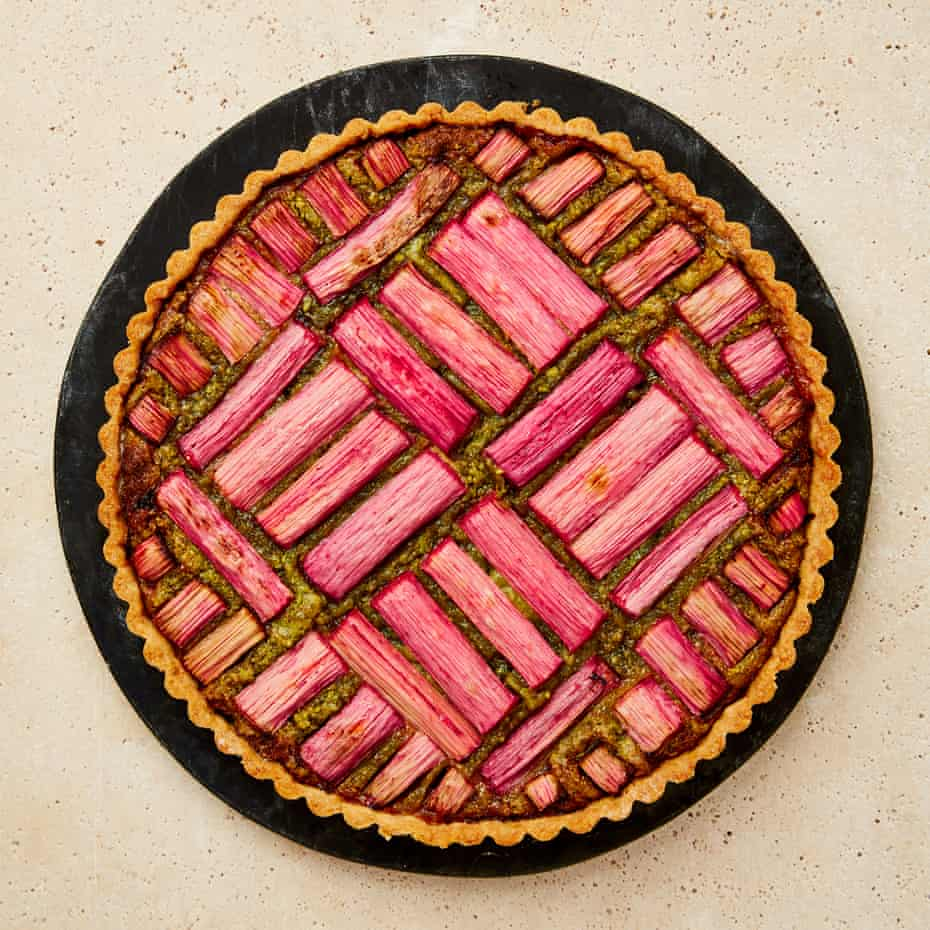
\includegraphics[width=10cm,height=10cm,keepaspectratio]{Recipe_Pictures/Rhubarb_and_pistachio_tart.png}
\end{figure}
\emph{I don’t believe in rules when it comes to the pairing of ingredients, but I removed rhubarb from its lifelong partner in crime, custard, with caution. Rhubarb by character is bright, fierce, acerbic and usually not for the faint-hearted unless tamed by something soothing. In custard’s place, I’ve used its more sophisticated cousin, frangipane, a sweet cream made using almonds, pistachios and oat milk flavoured with zesty orange and cardamom. (Though, if this makes you feel uncomfortable, and because there are no rules, you could always serve this tart with custard instead.)\\ 
Arrange the rhubarb as you wish: you could tessellate it (as per Instagram 2018) or just cut it into lengths. There are now some lovely vegan custards widely available – I like the ones made by both Alpro and Oatly.}\\\\ 
\textbf{Prep}: 10 min
\textbf{Cook}: 1 hr 45 min
\textbf{Rest}: 30 min
\textbf{Makes}: 1 x 23cm tart
\subsection*{Ingredients}
\begin{itemize}
\item For the pastry
\item 250g plain flour
\item 7 tbsp (105ml) light olive oil
\item 40g caster sugar
\item 1 pinch sea salt
\item 3 tbsp cold water
\end{itemize}

\begin{itemize}
\item For the filling
\item 7 tbsp (105ml) light olive oil
\item 125g caster sugar, plus 1 tbsp extra to finish
\item 50g cornflour
\item 200g ground pistachios
\item 40g ground almonds
\item 4 tbsp (60ml) oat milk
\item 1$\frac{1}{4}$ tsp cardamom powder
\item Zest of 1 orange
\item 250g forced rhubarb
\end{itemize}

\subsection*{Steps}
\begin{enumerate}
\item To make the pastry, put the flour, oil, sugar and salt in a bowl, and mix with a clean hand. Add the water, mix again, then knead for three minutes. Return to the bowl and refrigerate for 30 minutes.
\item Heat the oven to 200C (180C fan)/390F/gas 6. After the pastry has rested, put it between two sheets of baking paper and flatten it gently. Roll to about 3mm thick and just larger than a loose-bottomed 23cm tart tin. Peel off the top sheet of baking paper, put a hand under the bottom sheet and flip the pastry on top of the tart tin – don’t worry if it cracks or breaks. Reserve the baking paper. Press the pastry into place, cut away the overhang and use the offcuts to fill any cracks. Prick the base all over with a fork, crumple up one of the sheets of baking paper, unravel it and put it in the tart case. Fill with baking beans (or uncooked rice) and bake for about 25 minutes, until the pastry is crisp and lightly golden. Remove, and leave to cool.
\item To make the filling, mix everything except the rhubarb in a bowl until well combined, then set aside.
\item When the tart case is cool, lift out the baking paper and beans, and scrape the frangipane mix into the tart shell. Even it out and smooth it down with the back of a spoon. Now decorate as you wish: you could cut the rhubarb to size to lay stripes across the tart, or cut it into shorter lengths and tessellate. I like to do mine as in the photograph above by neatly arranging 6cm pieces of rhubarb at the centre of the tart, then filling the gaps around it with smaller pieces, cut to size.
\item Sprinkle the extra tablespoon of sugar all over the top of the rhubarb, then bake for 40-45 minutes, until the filling is starting to bronze slightly and the rhubarb is tender. Leave to cool a little before cutting and serving.
\end{enumerate}
\newpage

\section{Hasselback celeriac with miso and red onion}
\begin{figure}
\centering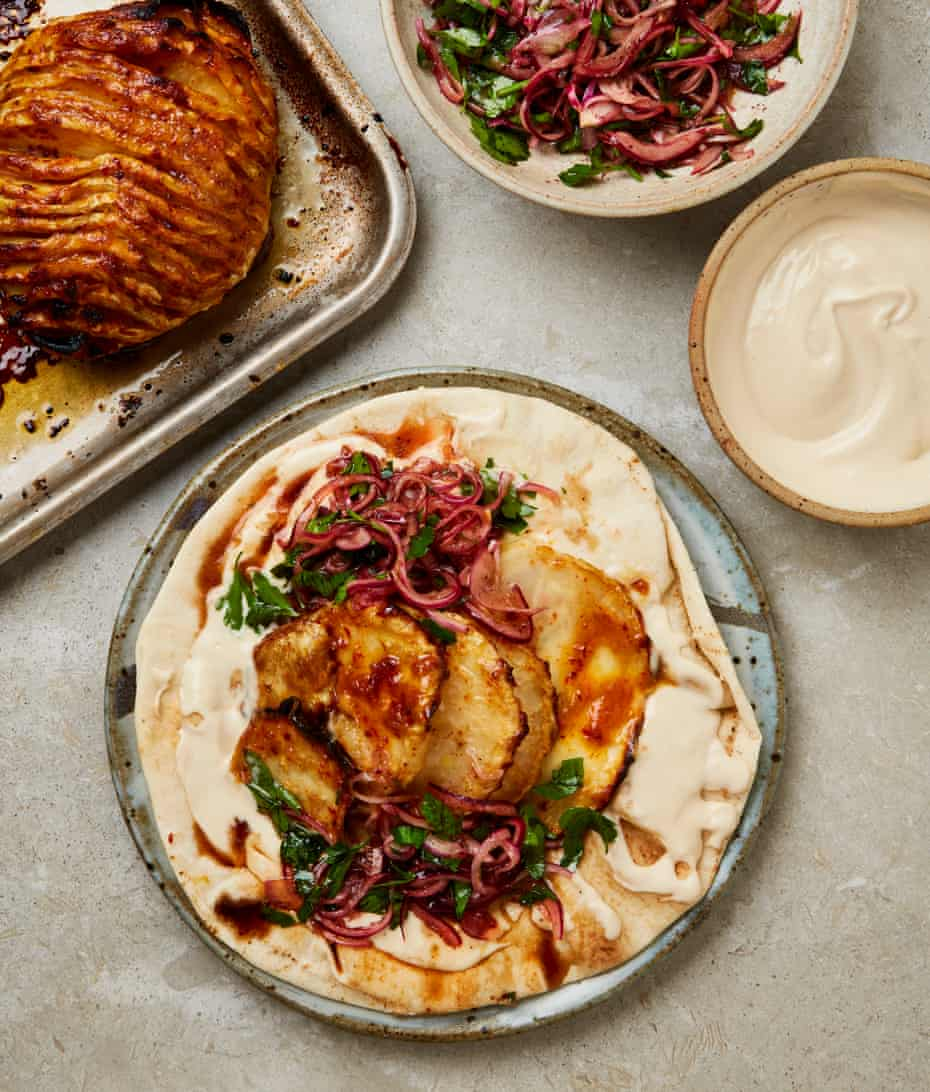
\includegraphics[width=10cm,height=10cm,keepaspectratio]{Recipe_Pictures/Hasselback_celeriac_with_miso_and_red_onion.png}
\end{figure}
\emph{The inspiration for a new dish can come from anywhere. In this case, I liked the sound of “hasselback celeriac” so much that I had to create a recipe just for the name. But now I am not sure I’ll ever be able to eat this root in any other way. Cutting deep fans into the celeriac means there’s more surface area to roast and to spread miso over, creating richer and deeper flavours, while the tops catch in the heat and crisp to a satisfying crunch. I have the brilliant Middle Eastern restaurant Bubala to thank for the special idea of combining celeriac, miso and tahini, and London’s many Turkish ocakbaşis for the sprightly pomegranate and onion salad.}\\\\ 
\textbf{Prep}: 10 min
\textbf{Cook}: 2 hr
\textbf{Serves}: 4
\subsection*{Ingredients}
\begin{itemize}
\item For the celeriac
\item 1 large or 2 small celeriac, about 1-1.2kg in total
\item 3-4 tbsp olive oil
\item 1 pinch salt
\end{itemize}

\begin{itemize}
\item For the miso glaze
\item 80g white miso – I like the Tideford Organics one
\item $\frac{1}{4}$ tbsp aleppo pepper
\item 2$\frac{1}{4}$ tbsp brown rice syrup
\item 1$\frac{1}{4}$ tbsp lemon juice
\end{itemize}

\begin{itemize}
\item For the tahini sauce
\item 100g tahini
\item 1 tbsp lemon juice
\item $\frac{1}{4}$ tsp salt
\end{itemize}

\begin{itemize}
\item For the salad
\item 1 red onion, peeled and cut into thin half-moons
\item 1 tbsp pomegranate molasses
\item 1 tbsp lemon juice
\item 1 tsp sumac
\item 3 tbsp olive oil
\item $\frac{1}{4}$ tsp salt
\item 1 large handful roughly chopped flat-leaf parsley
\end{itemize}

\begin{itemize}
\item To serve
\item Naan or flatbreads
\end{itemize}

\subsection*{Steps}
\begin{enumerate}
\item Heat the oven to 200C (180C fan)/390F/gas 6. Chop the base off the celeriac, peel off the skin using a peeler and use the tip of a knife to hoick out any unsightly muddy crevices. If the celeriac is large, cut it in half (if not, leave it whole), then, using a sharp knife, cut from top to bottom all over at $\frac{1}{4}$cm intervals down to 2cm from the base, then stop cutting.
\item Drizzle oil between the folds, rub more oil all over the top, and sprinkle with a tiny pinch of salt. Place on a nonstick tray, roast for 45 minutes, remove and, if need be, baste with a little more oil. Return to the oven and roast for another 45 minutes, until golden.
\item While the celeriac is cooking, make the miso glaze, tahini sauce and onion salad. Mix all the ingredients for the glaze in a small bowl and set to one side.
\item Put all the ingredients for the tahini sauce in a small serving bowl, whisk with five tablespoons of water and set to one side.
\item Combine all the salad ingredients in a serving bowl, scrunch together with your hands, to wilt the onions a little, and set to one side.
\item Once the celeriac is done, remove, carefully brush all over with the glaze – you want it to stay on the celeriac, not slip off – making sure it gets between the slits, then bake for a further 15 minutes, checking halfway through and possibly basting again with more glaze.
\item To serve, take the whole celeriac, pomegranate salad, tahini sauce and bread to the table, and encourage people to assemble it themselves with a smoosh of tahini on some bread, followed by a few slices of celeriac and a small tangle of pomegranate onions.
\end{enumerate}
\newpage

\section{Spring onion pancakes with sesame sauce}
\begin{figure}
\centering
\includegraphics[width=10cm,height=10cm,keepaspectratio]{Recipe_Pictures/Spring_onion_pancakes_with_sesame_sauce.png}
\end{figure}
\emph{ The world of pancakes is so vast, it is hard to think that on Pancake Day, there could be only one type proffered across the world. Of course, traditionally, pancakes were a way to use up eggs and animal fats before the Lent fast, but with those ingredients off the table in vegan cooking, a new array of pancakes can take centre stage. Today’s offering is for cong you bing, a flaky, coiled, spring onion pancake ubiquitous across China. It’s as enjoyable to make as it is to eat and, happily, there’s no whiff of abstinence about it.}\\\\ 
\textbf{Prep}: 5 min
\textbf{Cook}: 1 hr
\textbf{Rest}: 30 min
\textbf{Makes}: 4, to serve 2 for lunch
\subsection*{Ingredients}
\begin{itemize}
\item For the pancakes
\item 275g plain flour, plus 2 tbsp extra
\item Fine sea salt
\item Coconut oil
\item $\frac{1}{4}$ tsp Chinese five spice powder – I like Bart Ingredients 
\item 6 spring onions, trimmed and finely sliced
\end{itemize}

\begin{itemize}
\item For the sesame sauce
\item 30g tahini
\item 75g sweet white miso – I like Clearspring
\item 1 tbsp toasted sesame oil
\item 2 tbsp white-wine vinegar
\item $\frac{1}{4}$ tsp chilli oil sediment plus 1 tbsp oil – I like Lee Kum Kee
\end{itemize}

\subsection*{Steps}
\begin{enumerate}
\item Making these involves a particular set of processes that includes binding, rolling, folding, squashing and frying. I would have had trouble learning them by myself during the pandemic were it not for the help of a library of online cooks, and in particular Wei Guo of the wonderful Red House Spice blog.
\item Fill and boil half a kettle of water. In a large heatproof bowl, use a fork to mix the flour, a big pinch of salt and 165ml freshly boiled water until it comes together into a rough dough and is cool enough to handle. Knead for five minutes, then cover with a clean tea towel and set aside to rest for 30 minutes.
\item While the dough is resting, prepare the filling. Melt two tablespoons of coconut oil in a nonstick pan, then pour into a small heatproof bowl. Put the pan to one side, but don’t wash it up – you’ll use it again later, to cook the pancakes. Add the five spice, the two extra tablespoons of flour and a quarter-teaspoon of salt to the melted oil, stir to combine and set aside.
\item Mix all the sauce ingredients in a small bowl, add two tablespoons of cold water to loosen it a little, and set aside.
\item Once the dough has rested, rub a little coconut oil on a worktop and on a rolling pin, then roll the dough into a roughly 20cm x 30cm rectangle. Spread the five spice mix evenly over the top (take care not to tear the dough) and sprinkle the sliced spring onions on top of that. Starting at one short end of the dough rectangle, roll up the whole thing into a tight cigar. Move the dough sausage so it’s horizontally in line with the edge of the worktop, then cut into four even slices. Put the slices cut side down on the worktop and, using the greased rolling pin, gently press each slice into a round pancake shape measuring about 13cm across.
\item When you are ready to cook the pancakes, melt two tablespoons of coconut oil in the nonstick pan, gently lift in one pancake and cook for three to four minutes on each side, until golden brown all over. Remove from the pan and keep somewhere warm while you repeat with the remaining oil and pancakes (keep a close eye on the heat under the pan – you may need to reduce it to make sure the pan doesn’t get too hot).
\item Serve the pancakes hot with the sauce for dipping or drizzling over the top.
\end{enumerate}
\newpage

\section{Maham’s dal}
\begin{figure}
\centering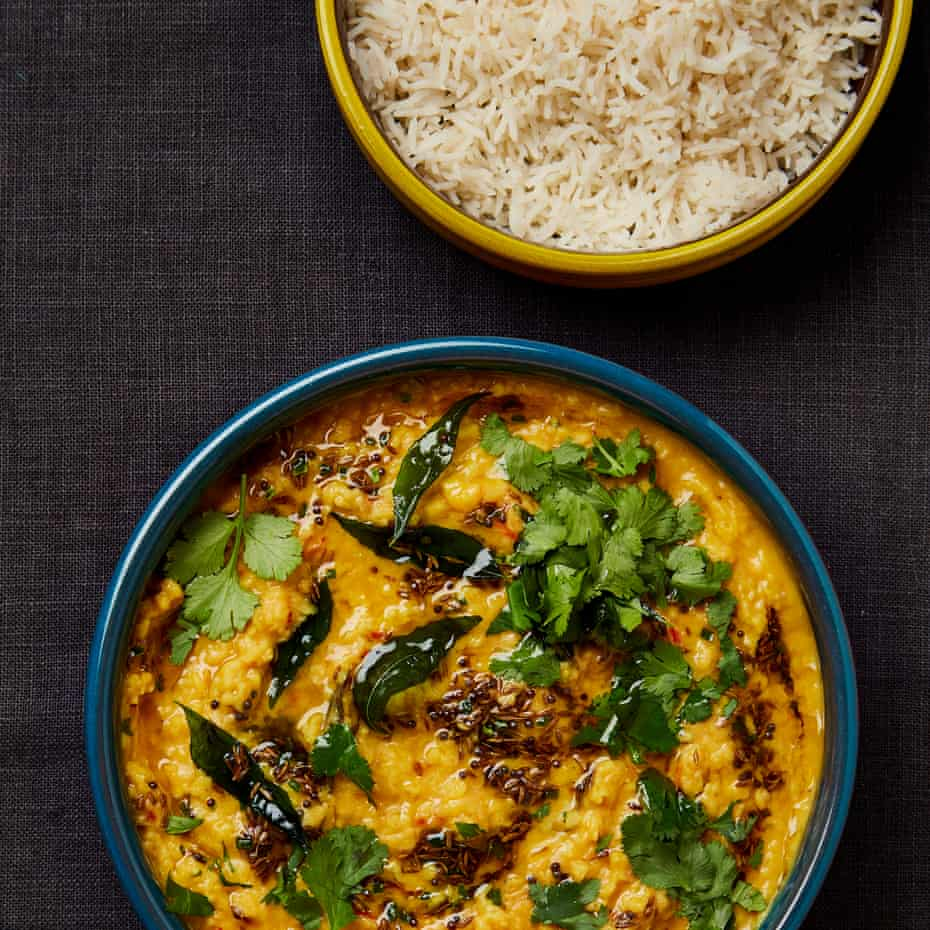
\includegraphics[width=10cm,height=10cm,keepaspectratio]{Recipe_Pictures/Mahams_dal.png}
\end{figure}
\emph{There’s a lot to love about ceramicist Maham Anjum. Her hands that move with well-practised grace on her pottery wheel, moulding large, unfriendly-looking boulders of clay into elegant bowls and biryani pots. Her rickety, wooden studio in the midst of an overgrown garden that’s filled in summer with hollyhocks, butterflies and a curious little fox. \\ 
Her work, of course, out of which we ate this heavenly dal. And the manner in which she introduced it: ‘I just put it all in a pot and stir it.’ It’s that simple, and now it is one of my favourite things to make and eat most weeks.\\ 
This dal, which has been photographed in one of Maham’s handmade bowls, is made with the very quick-cooking mung dal, which are the de-husked, split yellow insides of green mung beans – look for it in big supermarkets or Asian food shops. Since this recipe was first published in East, I’ve adapted it by cooking out the tomatoes and garlic first, though Maham just throws them into the pot with everything else.}\\\\ 
\textbf{Prep}: 10 min
\textbf{Cook}: 45 min
\textbf{Serves}: 4
\subsection*{Ingredients}
\begin{itemize}
\item Rapeseed oil
\item 3 fat garlic cloves, peeled and minced
\item 2.5cm piece fresh ginger, peeled and grated
\item 250g vine tomatoes, (ie, 3 medium ones), chopped
\item 300g mung dal
\item $\frac{1}{4}$ tsp turmeric
\item 1 tsp chilli flakes
\item 12 fresh curry leaves
\item 1$\frac{1}{4}$ tsp salt
\item 1 tsp cumin seeds
\item $\frac{1}{4}$ tsp black mustard seeds
\item 1 green finger chilli, very finely chopped
\item 1 handful fresh coriander, roughly chopped, to serve
\end{itemize}

\subsection*{Steps}
\begin{enumerate}
\item In a large saucepan, heat two tablespoons of oil over a medium heat and, when hot, add the garlic and ginger, and cook for three minutes, until they turn a pale shade of gold. Add the tomatoes, cook for five to six minutes, then add the dal, turmeric, chilli flakes, four of the curry leaves and a litre and a quarter of water. Put a cocked lid on top of the pan and bring to a boil. Turn down the heat to a simmer, leave the dal to cook, stirring every now and then, for 30-40 minutes, until soft and fairly thick, then stir in the salt.
\item When the dal is nearly cooked, make the tarka. Heat two tablespoons of oil in a small frying pan over a medium heat and, when it’s smoking hot, add the cumin seeds, mustard seeds, green chilli and remaining eight curry leaves. When the leaves crisp up and the seeds crackle, which should happen within the first minute, take the tarka off the heat and pour into the dal. Stir to mix, sprinkle over the coriander and serve with freshly steamed basmati rice.
\end{enumerate}
\newpage

\section{Chocolate chip cookies}
\begin{figure}
\centering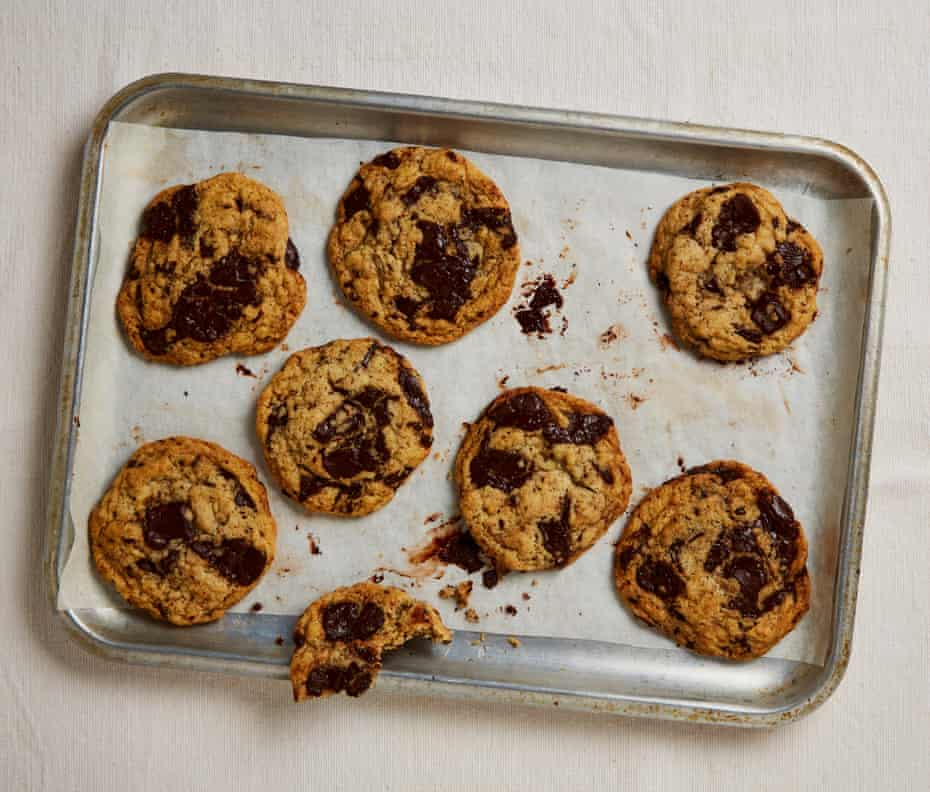
\includegraphics[width=10cm,height=10cm,keepaspectratio]{Recipe_Pictures/Chocolate_chip_cookies.png}
\end{figure}
\emph{The biscuits of my youth – bourbons, custard creams and digestives – were crisp, smooth and crunchy until America arrived in my life some time in my teens. Then, everything changed. \\ 
I spent Friday nights watching Friends, I listened to NWA on my Sony Walkman, wore tie-dye T-shirts and drank ‘thick shakes’. Crucially, when it came to biscuits, crisp was most definitely out and big, soft and chewy cookies were in. They made quite the impression and, if I’m honest, never really left – I am still a cookie-lover, so I thought it about time I wrote a recipe for this American classic.}\\\\ 
\textbf{Prep}: 10 min
\textbf{Cook}: 25 min
\textbf{Rest}: 30 min
\textbf{Makes}: 16
\subsection*{Ingredients}
\begin{itemize}
\item 200g plain flour
\item $\frac{3}{4}$ tsp baking powder
\item $\frac{1}{4}$ tsp bicarbonate of soda
\item $\frac{1}{4}$ tsp sea salt, crumbled
\item 150g golden caster sugar
\item 125g 70\% dark chocolate
\item 85ml sunflower oil – I like Mr Organic
\item 2 tsp vanilla extract
\end{itemize}

\subsection*{Steps}
\begin{enumerate}
\item Put the flour, baking powder, bicarb, salt and sugar in a large bowl and mix well. Break the chocolate into little chunks, add these to the bowl and mix again.
\item In a small bowl, briskly whisk the oil, vanilla extract and four tablespoons of water, until emulsified. Pour the liquids into the dry ingredients, stir vigorously with a wooden spoon until the mixture comes together into a batter, then pop the bowl in the fridge for at least 30 minutes.
\item Heat the oven to 190C (180C fan)/390F/gas 6 and line two large oven trays with baking paper. Using a small scoop – for example a tablespoon measuring spoon – spoon the cookie dough on to the sheet, spacing the rounds 10cm apart, because they’ll spread. (If you don’t have a suitable scoop, gently roll the dough with your hands into balls the size of ping-pong balls and weighing about 40g each.)
\item Bake for 12 minutes, or until the cookies have a crisp, golden edge and are not wobbly to the touch in the centre. Leave to cool completely on the trays before eating. Store any leftovers (as if!) in an airtight container.
\end{enumerate}
\newpage

\section{Miso mushrooms on toast}
\begin{figure}
\centering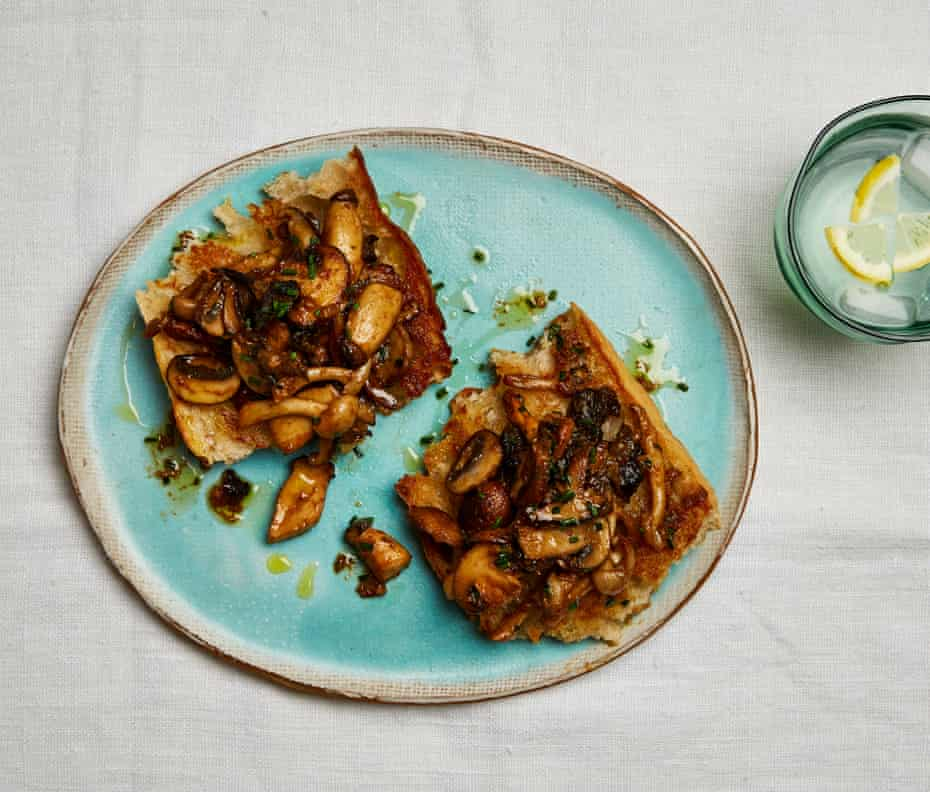
\includegraphics[width=10cm,height=10cm,keepaspectratio]{Recipe_Pictures/Miso_mushrooms_on_toast.png}
\end{figure}
\emph{Cooking for myself is one of my favourite things. There is no dinner by consensus and no fussy eaters to consider (except myself). I can choose whether to eat just a little or obscene amounts, add extra heat or perhaps lick the plate afterwards. And I can do it all while watching series two of Sex Education on Netflix.\\ 
When the opportunity arises, I like to make something by foraging in the fridge and the cupboard, and the formula goes a bit like this: something fresh (like mushrooms) with some quick flavour (miso) on toast. Always toast.}\\\\ 
\textbf{Prep}: 5 min
\textbf{Cook}: 10 min
\textbf{Serves}: 1
\subsection*{Ingredients}
\begin{itemize}
\item Light olive oil 
\item 1 reasonable hunk ciabatta, halved 
\item 1 tsp brown rice miso
\item 2 tsp white shiro miso 
\item 200g mushrooms – a mixture of wild and chestnut mushrooms, sliced
\item 2 garlic cloves, peeled and crushed 
\item 10 chives, very finely sliced
\end{itemize}

\subsection*{Steps}
\begin{enumerate}
\item First toast the bread. Set a large, nonstick frying pan on a medium to high heat and drizzle a little oil over both sides of the bread. When hot, fry the bread for two to three minutes on each side, until golden, then transfer to a plate.
\item Put the two miso pastes in a small bowl, add two tablespoons of water, mix to combine and set aside.
\item Using the same pan, heat a couple of tablespoons of oil over a medium to high flame and, when hot, add the mushrooms, making sure they all have room to cook. Leave to cook undisturbed for four minutes, until they turn a shade of golden brown, then stir in the garlic and cook for another two minutes.
\item Pour in the miso mixture – be careful, it may splatter – and turn the heat right down. The mixture will quickly bubble up and the liquid frazzle away, and you’ll be left with a thick glaze around the mushrooms. Stir in the chives, then tip the lot on to the ciabatta. Drizzle with a little oil, if you wish, and serve immediately.
\end{enumerate}
\newpage

\section{Rose harissa chickpea stew with burnt chard}
\begin{figure}
\centering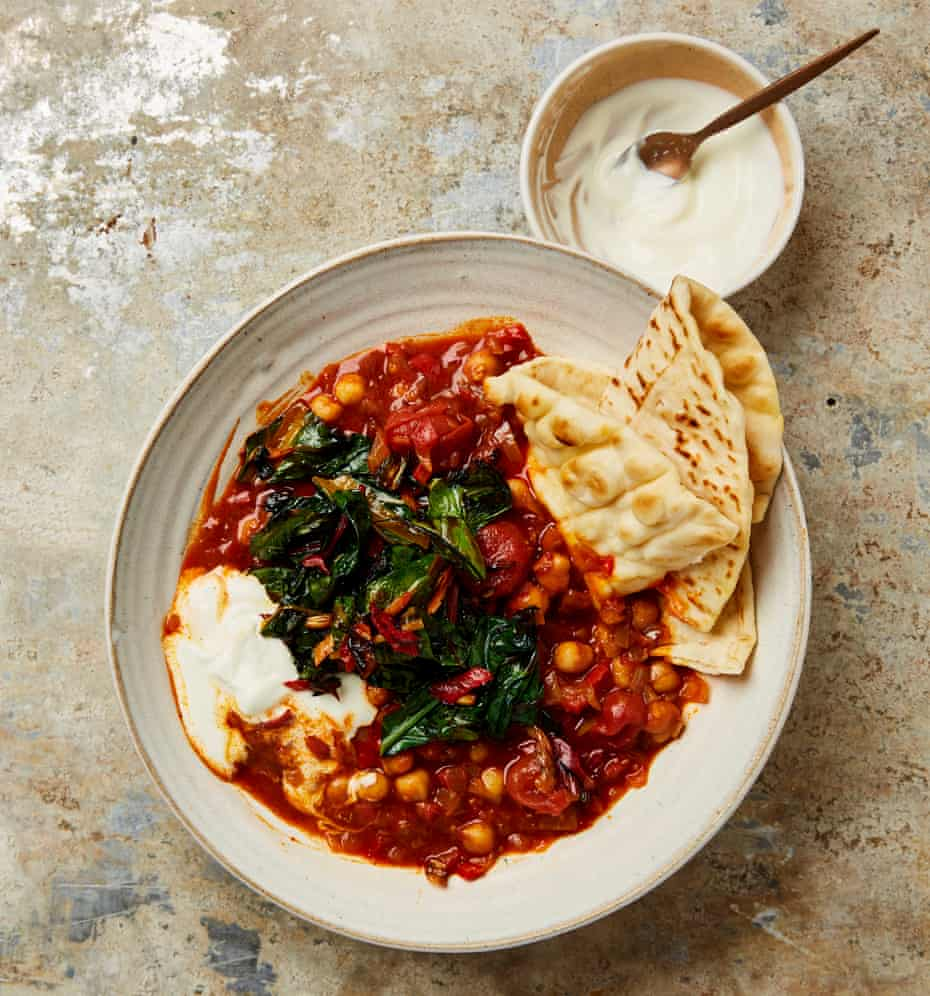
\includegraphics[width=10cm,height=10cm,keepaspectratio]{Recipe_Pictures/Rose_harissa_chickpea_stew_with_burnt_chard.png}
\end{figure}
\emph{Rose harissa is the equivalent of a friend who always brings the party, no matter the situation. A friend, in all honesty, to whom I hadn’t paid much attention until I spotted a recipe (of which this is a bit of a wild adaptation) in Elly Curshen’s latest book, Green.\\ 
In it, the sweet smoke and spiciness of rose harissa gets store-cupboard staples such as chickpeas, tinned tomatoes and onions dancing to a great rhythm with very little fuss, and lots of wonderful flavour.}\\\\ 
\textbf{Prep}: 15 min
\textbf{Cook}: 45 min
\textbf{Serves}: 4
\subsection*{Ingredients}
\begin{itemize}
\item 1 tsp cumin seeds
\item Rapeseed oil
\item 2 onions, peeled and finely chopped
\item 2 red peppers, stems, pith and seeds removed, flesh finely chopped
\item 3 fat garlic cloves, peeled and minced
\item 1$\frac{1}{4}$ tbsp tomato puree
\item 2$\frac{1}{4}$ tbsp rose harissa – I like Belazu’s (if you’re on a gluten-free diet, check the label, because not all brands are GF)
\item Fine sea salt
\item 1$\frac{1}{4}$ tsp ground sweet paprika
\item 1 x 400g tin cherry tomatoes
\item 2 x 400g tin chickpeas, not drained
\item 200g rainbow chard, stems finely sliced, leaves roughly chopped, kept separate
\item $\frac{1}{4}$ tbsp lemon juice
\end{itemize}

\begin{itemize}
\item To serve
\item Flatbread
\item Non-dairy yoghurt (optional)
\end{itemize}

\subsection*{Steps}
\begin{enumerate}
\item Coarsely bash the cumin in a mortar and set to one side. Put three tablespoons of oil in a large casserole pot on a medium heat and, once hot, add the onions and peppers. Fry, stirring from time to time, for 20 minutes, until soft. Stir in the garlic, tomato puree, harissa, a teaspoon of salt, the paprika and bashed cumin seeds, cook for five minutes more, then add the tomatoes and cook for another 10 minutes. 
\item Add the chickpeas and the liquid from their tin, turn down the heat to a simmer and leave to bubble away for about 10 minutes, by which time the chickpeas should be nice and soft and the stew rich and flavourful; if not, keep cooking for another five or so minutes.
\item To cook the chard, heat a tablespoon of oil in a wide frying pan over a high heat and, when the oil is shimmering, add the chard stems and fry, stirring once, for two minutes, until charred all over. Add the leaves, leave them to blister for two minutes, then turn and leave for another two minutes. Take off the heat, add the lemon juice and salt to taste, and toss.
\item To serve, heat up the flatbread. Ladle the stew into shallow bowls, fold the hot flatbread into quarters and put to one side. Put a little pile of chard on top of the chickpeas and add a dollop of non-dairy yoghurt, if you like.
\end{enumerate}
\newpage

\section{Soba noodle soup with caramelised cabbage and pickles}
\begin{figure}
\centering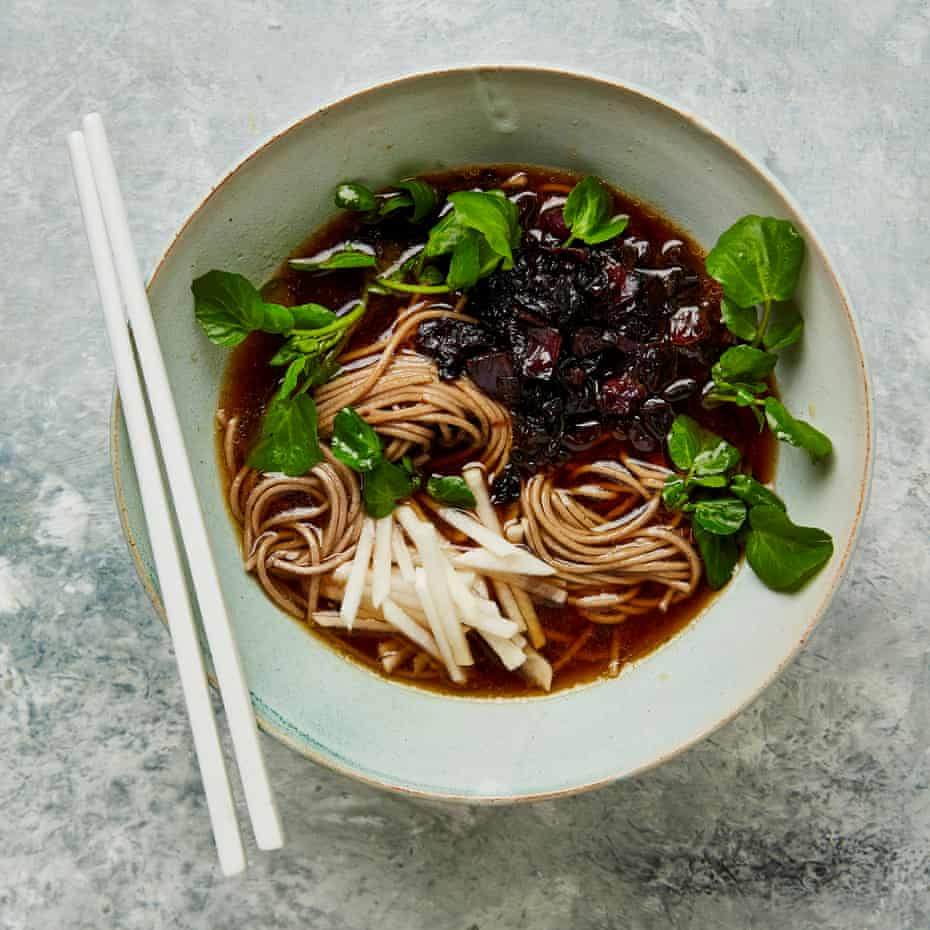
\includegraphics[width=10cm,height=10cm,keepaspectratio]{Recipe_Pictures/Soba_noodle_soup_with_caramelised_cabbage_and_pickles.png}
\end{figure}
\emph{This soup is based on the Japanese toshikoshi soba soup, or ‘year-crossing noodle’, a piping-hot noodle soup packed with symbolism.\\ 
Traditionally, it’s eaten on New Year’s Eve to reflect on the past year and welcome the new one, but it’s never too late. The idea is to enjoy a long, peaceful life with each slurp and break free from the past as the noodle breaks easily with each bite. In its simplest form it is made using buckwheat soba noodles and a hot dashi broth, but I’ve taken liberties and bolstered it with soy-caramelised cabbage and some turnip pickles.\\ 
Turnips can be hard to find, so if you can’t get hold of any, use beetroot instead. Kombu is available from Asian supermarkets or online. There are pure buckwheat soba noodles and those mixed with wheat: I find the latter easier to work with – Clearspring make good ones, and they’re available in large supermarkets.}\\\\ 
\textbf{Prep}: 20 min
\textbf{Cook}: 1 hr
\textbf{Serves}: 4
\subsection*{Ingredients}
\begin{itemize}
\item For the cabbage
\item 2 tbsp rapeseed oil 
\item 1 large red cabbage (around 800g), cored and chopped into 1cm pieces 
\item 1 red onion, peeled and finely chopped 
\item 4 tbsp mirin 
\item 1 tbsp rice vinegar 
\item 1 tsp fine sea salt
\end{itemize}

\begin{itemize}
\item For the soup
\item 1 large piece kombu (about 50g)
\item 4 tbsp brown rice miso 
\item 4 tbsp light soy sauce
\item 4 tbsp mirin 
\item 200g soba noodles 
\item 2 tbsp toasted sesame oil 
\item 60g watercress, stalky ends removed
\end{itemize}

\begin{itemize}
\item For the turnip pickle
\item 2 small turnips (around 200g), peeled, cut into thick matchsticks 
\item $\frac{1}{4}$ tsp fine sea salt 
\item 100ml rice vinegar
\end{itemize}

\subsection*{Steps}
\begin{enumerate}
\item Start with the cabbage. Heat a large frying pan on a medium heat, add the oil, then the cabbage and onion, and cook, stirring occasionally to stop it sticking, for 30 minutes. Add the mirin, vinegar and salt, and cook for 20 minutes more, by which time the cabbage should be caramelised and very tender.
\item While the cabbage is cooking, get the soup base started. In a medium saucepan, bring one and a half litres of water to a boil, lower the heat to a whisper, add the kombu and simmer for 10 minutes. Carefully remove the kombu with a pair of tongs and discard. Whisk the miso, soy sauce and mirin into the hot broth and leave to one side.
\item Next, pickle the turnips. In a jug, mix the salt into the vinegar and 100ml freshly boiled water, then pour over the turnip in a heatproof bowl and set aside.
\item Cook the buckwheat noodles according to the packet instructions, taking a minute off the cooking time, then drain and rinse under cold water. Transfer to a bowl and mix through the toasted sesame oil.
\item To assemble, divide the noodles between four bowls. Gently heat up the broth, pour it over the noodles, then top with the caramelised soy cabbage, watercress and pickled turnips, and serve.
\item  This article was amended on 3 February 2020, to clarify the description of the cabbage. An earlier version described it as “soy cabbage”. In addition, the recipe’s name has been amended to remove “ginger”, which was included in error. 
\end{enumerate}
\newpage

\section{Pistachio, chilli and lemon spaghetti}
\begin{figure}
\centering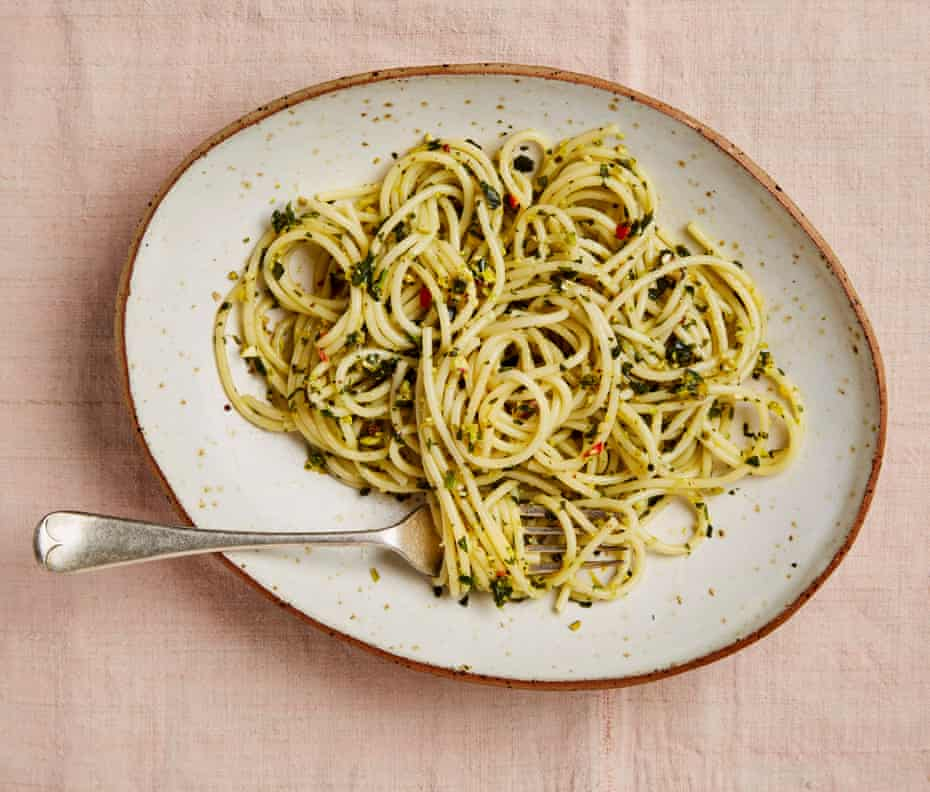
\includegraphics[width=10cm,height=10cm,keepaspectratio]{Recipe_Pictures/Pistachio,_chilli_and_lemon_spaghetti.png}
\end{figure}
\emph{You might know by now that I’m fond of chillies, and the thing about chilli-fondness is that I need a hit on an almost daily basis. I find it affects other cuisines I cook, too, such as Italian food, and this spaghetti, for example. It’s (very) loosely inspired by a plate of salsa di pistacchi pasta I had in Sicily, but I’ve injected the roaring streets of Bangkok into it by way of a couple of bird’s eye chillies.\\ 
If you’re not as fond of heat as I am, add as much chilli as you’re comfortable with.}\\\\ 
\textbf{Prep}: 5 min
\textbf{Cook}: 12 min
\textbf{Serves}: 4
\subsection*{Ingredients}
\begin{itemize}
\item Salt 
\item 100g fresh basil, leaves picked
\item 1 garlic clove, peeled
\item 100g pistachios
\item 2 red bird’s eye chillies
\item Zest and juice of 1 lemon
\item 80ml olive oil
\item 400g spaghetti
\end{itemize}

\subsection*{Steps}
\begin{enumerate}
\item Put a large pan of water on to boil and add two teaspoons of salt for every litre of water. In the meantime, finely chop the basil, and do the same with the garlic, pistachios and chilli. Run the knife repeatedly over all the chopped ingredients, until they’re very, very fine, then transfer to a large bowl. Add the lemon zest, three tablespoons of lemon juice, the olive oil (if you like, use a little more, to loosen the sauce) and half a teaspoon of salt (or to taste), and mix well.
\item Cook the pasta in the boiling water for seven minutes (or according to packet instructions), until al dente. Scoop out 100ml or so of the pasta water with a ladle, then drain the pasta. Add the cooked pasta to the pesto bowl, toss to coat thoroughly, adding a little pasta water, if necessary, to loosen the sauce, then serve.
\end{enumerate}
\newpage

\section{Potato, aubergine and spinach curry}
\begin{figure}
\centering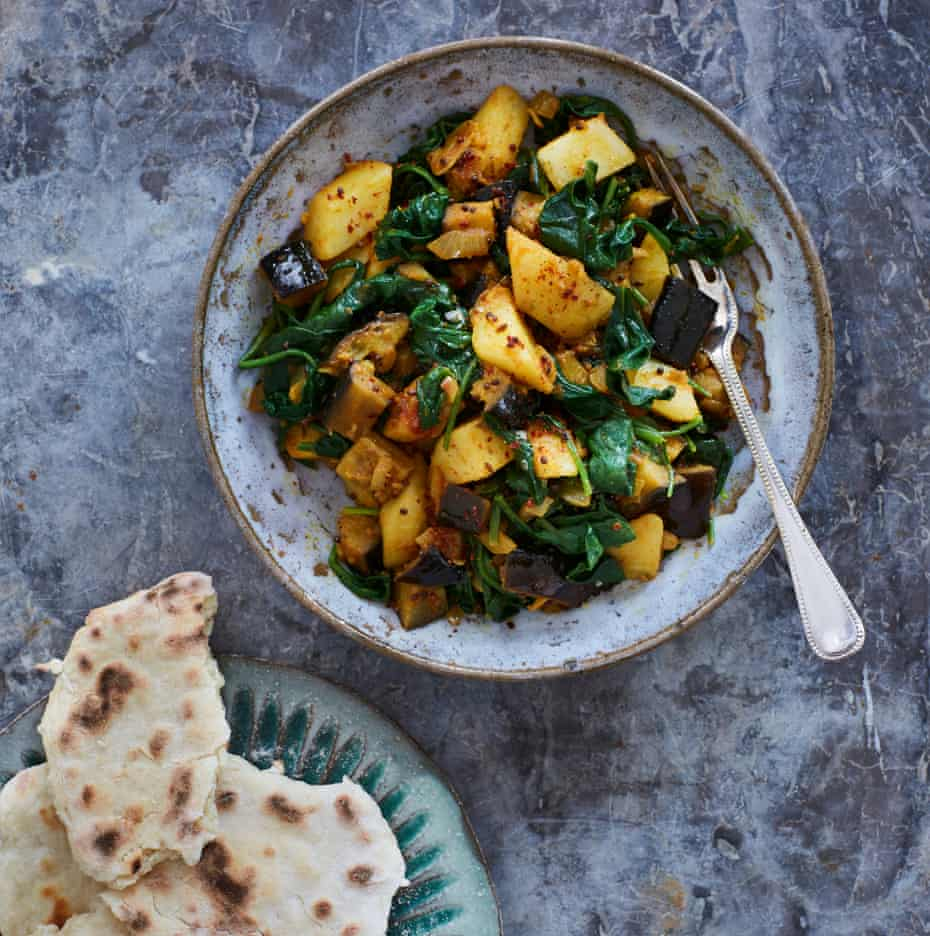
\includegraphics[width=10cm,height=10cm,keepaspectratio]{Recipe_Pictures/Potato,_aubergine_and_spinach_curry.png}
\end{figure}
\emph{I recently had the privilege of judging the Andre Simon Awards for the best food book of 2018, and 119 books turned up, box by box, at my door (thank you, postman). Although there are some mind-blowing new books among them – the winner Diana Henry’s included – I thought to myself: ‘How many recipes does one person need?’ Of course, I am charged with writing new recipes here every week, but so often I’ll find that my pitch-perfect meal is something simple that I grew up eating - which is what today’s recipe is: a classic saag aloo, with added aubergine for extra oomph.\\ 
The only thing this recipe lacks is looks, but try not to hold that against it.}\\\\ 
\textbf{Prep}: 10 min
\textbf{Cook}: 25 min
\textbf{Serves}: 4
\subsection*{Ingredients}
\begin{itemize}
\item 750g maris piper potatoes, peeled
\item Salt
\item 4 tbsp rapeseed oil
\item 1$\frac{1}{4}$ tsp cumin seeds 
\item 1 tsp black mustard seeds 
\item 1 aubergine, cut into 1cm dice
\item 1 large brown onion, peeled and very finely chopped
\item 2$\frac{1}{4}$cm piece fresh ginger, peeled and very finely chopped 
\item 4 garlic cloves, peeled and very finely chopped
\item $\frac{1}{4}$ tsp turmeric
\item 1$\frac{1}{4}$ tsp Kashmiri chilli powder 
\item 1$\frac{1}{4}$ tsp ground coriander 
\item 2 tbsp tomato puree 
\item 400g baby spinach, washed
\end{itemize}

\subsection*{Steps}
\begin{enumerate}
\item Cut the potatoes into bite-sized pieces roughly 3cm square, put these into a medium saucepan, add a teaspoon of salt and cover with plenty of cold water. Bring to a boil, cook until just tender – around eight to 10 minutes – then drain.
\item Meanwhile, pour the oil into a large, deep-sided frying pan for which you have a lid, and put over a medium heat. Add the cumin and mustard seeds to the hot oil and watch carefully: when they start to sizzle, add the diced aubergine, onion and a teaspoon of salt.
\item Turn down the heat a little and cook until the onions and aubergines are soft enough to cut with a wooden spoon and starting to brown – about 10 minutes. Now stir in the ginger and garlic and, after a few more minutes, the turmeric, chilli powder and ground coriander. Mix in the tomato paste, turn the heat to low, cook for a further 10 minutes, then add the drained potatoes and stir gently so as not to crush them.
\item Add a big handful of spinach, stir, add a splash of water and cover with the lid – it will take a few minutes to wilt down. Repeat until all the spinach is wilted and soft. Add a couple of tablespoons of water, mix and cook for two to three minutes more, then take off the heat.
\item Serve with chapatis or naan, yoghurt and a little lime or lemon pickle on the side.
\end{enumerate}
\newpage

\section{Aubergine fesenjan}
\begin{figure}
\centering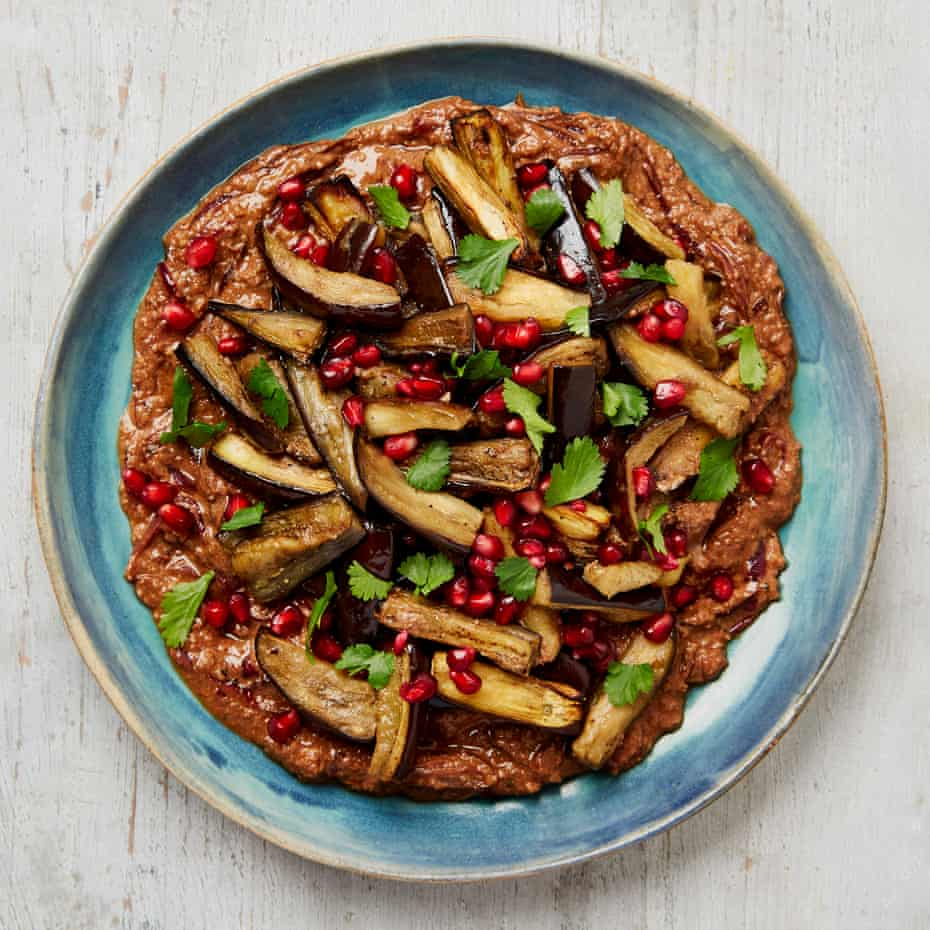
\includegraphics[width=10cm,height=10cm,keepaspectratio]{Recipe_Pictures/Aubergine_fesenjan.png}
\end{figure}
\emph{The first thing I noticed about my now-husband Hugh when we met wasn’t his beautiful face or wit, but the hugely disconcerting red splatters over him and his kitchen’s walls. He’d been juicing pomegranates to make me this ancient Persian dish, in which walnuts and pomegranates combine to make a rich, tart and sweet sauce. These days, you can buy pomegranate molasses everywhere, which is what we use when we make this dish now to celebrate our relationship (and save the walls).\\ 
This recipe is from my book Fresh India. You’ll need a food processor to grind the walnuts.}\\\\ 
\textbf{Prep}: 10 min
\textbf{Cook}: 30-35 min
\textbf{Serves}: 4 as a main
\subsection*{Ingredients}
\begin{itemize}
\item 120g walnuts
\item 4 medium aubergines (1.2 kg)
\item Rapeseed oil
\item Salt and ground black pepper
\item 2 large red onions, peeled and thinly sliced
\item 2 garlic cloves, peeled and crushed
\item 1$\frac{1}{4}$ tbsp brown rice syrup
\item $\frac{3}{4}$ tsp chilli powder
\item 1 tsp ground cinnamon
\item 2 tbsp pomegranate molasses
\item 250ml hot vegetable stock
\item Seeds from 1 pomegranate
\item 1 handful fresh coriander, roughly chopped
\end{itemize}

\subsection*{Steps}
\begin{enumerate}
\item Heat the oven to 200C (180C fan)/390F/gas 6 and line a large baking tray with lightly oiled foil. In a food processor, blitz the walnuts to a fine crumb.
\item Cut the aubergines into 5cm x 2cm batons, toss in a bowl with a little oil to coat, season lightly, then transfer to the prepared tray and roast for 25 minutes, until meltingly soft.
\item While the aubergines are roasting, make the fesenjan sauce. Put three tablespoons of oil into a large frying pan over a medium heat and, once hot, add the onions and fry for 12 minutes, stirring regularly to ensure they don’t catch. 
\item Add the garlic, fry for three minutes, then stir in the brown rice syrup, chilli powder, cinnamon, half a teaspoon of salt, a teaspoon of ground black pepper, the blitzed walnuts and the pomegranate molasses. Pour in the stock and cook for about eight minutes, until the sauce comes together.
\item When the aubergines are tender, pour the sauce into a serving dish. Arrange the aubergines on top, scatter over the pomegranate seeds and coriander, and serve with steamed basmati rice.
\end{enumerate}
\newpage

\section{Iraqi white bean stew (fasoulia)}
\begin{figure}
\centering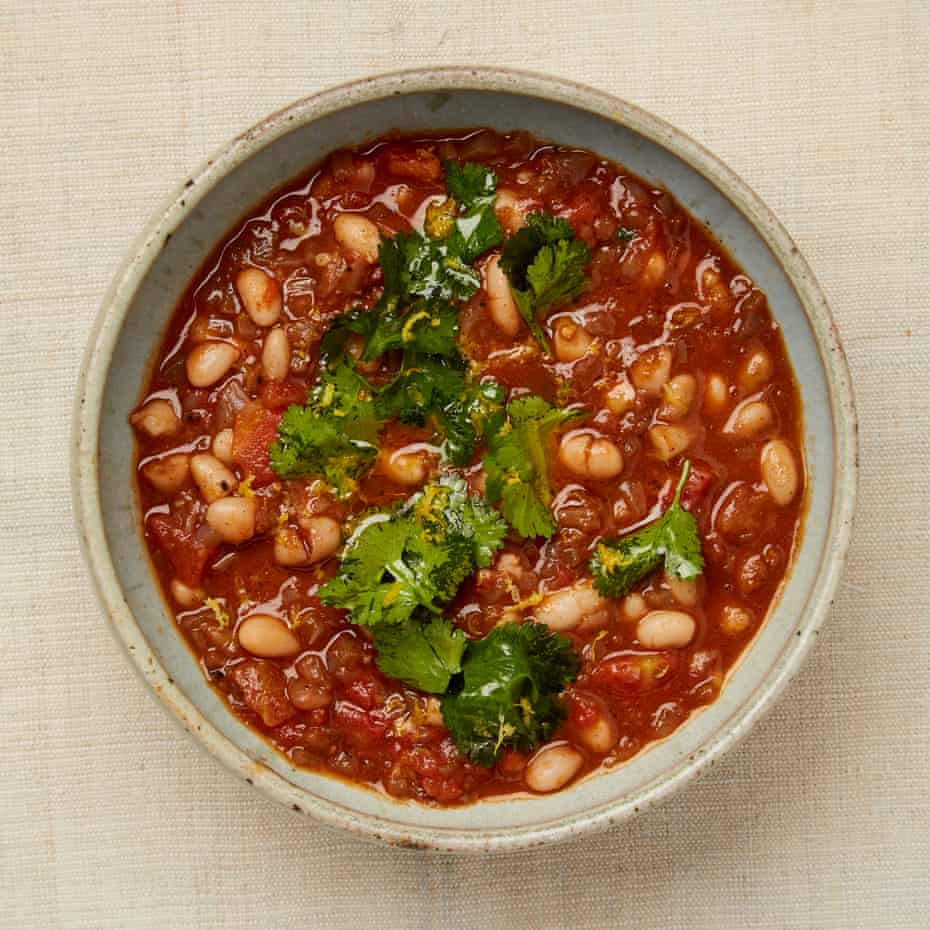
\includegraphics[width=10cm,height=10cm,keepaspectratio]{Recipe_Pictures/Iraqi_white_bean_stew_(fasoulia).png}
\end{figure}
\emph{In the middle of the Venn diagram between my head, heart and stomach are these beans. I long for them, I love them and I cooked them several times over Christmas and new year after talking to my British-Iraqi friend Assallah’s mother, Amina, about them. They’re essentially cannellini beans in a spiced tomato sauce topped with a sprightly, lemony coriander oil. But they are also more than that: they are a taste of home.\\ 
Amina uses a pre-bought Iraqi seven-spice mix called baharat in her recipe, which you could use instead of the spices in mine.}\\\\ 
\textbf{Prep}: 10 min
\textbf{Cook}: 30 min
\textbf{Serves}: 4
\subsection*{Ingredients}
\begin{itemize}
\item Rapeseed oil, for frying
\item 2 brown onions, peeled and finely chopped
\item Salt
\item $\frac{1}{4}$ tsp ground black pepper 
\item $\frac{1}{4}$ tsp ground cinnamon 
\item 1 tsp ground allspice
\item $\frac{1}{4}$ tsp ground cumin
\item 50g fresh coriander, picked, stalks finely chopped
\item 1 x 400g tin chopped tomatoes
\item 2 x 400g tins cannellini beans, drained and rinsed
\item 1 lemon, zested, and juiced, to give about 3 tbsp lemon juice
\end{itemize}

\subsection*{Steps}
\begin{enumerate}
\item Heat three tablespoons of oil in a large, heavy-bottomed saucepan on a medium heat. Once hot, add the onions, a teaspoon of salt, the black pepper, cinnamon, allspice, cumin and coriander stalks, and cook, stirring occasionally, for 20 minutes, until soft and dark. Keep an eye on it, because you don’t want the onions or spices to catch.
\item When the mix is soft and sweet-smelling, add the tomatoes, beans and 200ml water, bring up to a boil, then simmer for 10 minutes.
\item In a bowl, mix two tablespoons of rapeseed oil, the coriander leaves, lemon zest and juice, and a quarter-teaspoon of salt.
\item To serve, divide the stew between four bowls and top with a generous spoonful of the coriander and lemon oil.
\end{enumerate}
\newpage

\section{Wild rice kitchari with baked yoghurt and chilli seeds}
\begin{figure}
\centering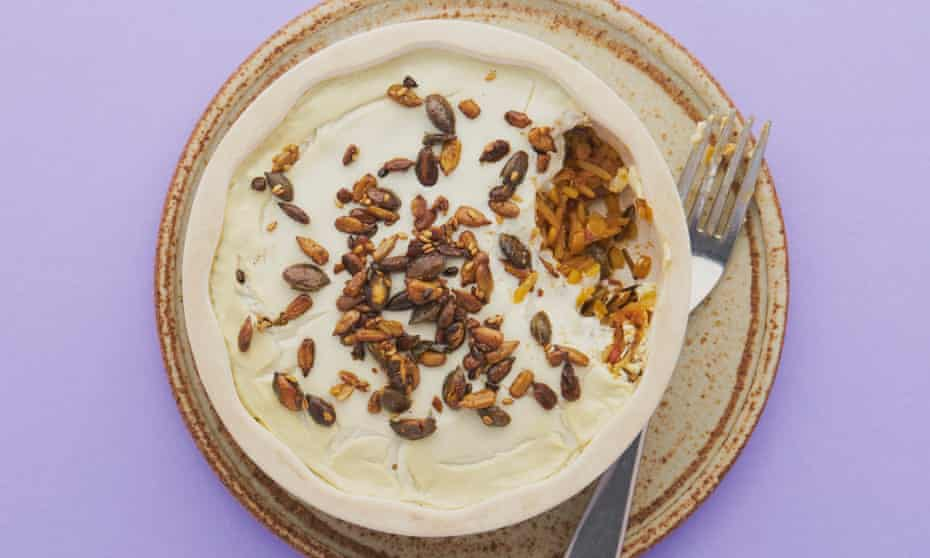
\includegraphics[width=10cm,height=10cm,keepaspectratio]{Recipe_Pictures/Wild_rice_kitchari_with_baked_yoghurt_and_chilli_seeds.png}
\end{figure}
\emph{Kitchari is a centuries-old rice and lentil dish that’s still eaten across India. Precursor of the Anglo-Indian favourite kedgeree and the Egyptian street food koshari, it’s the country’s original one-pot dish, and both seasonal and endlessly adaptable. This recipe is inspired by one I ate at Swati Snacks in Mumbai, a restaurant with strip lighting, laminated menus and a long queue: the telltale sign of a place everyone wants to eat at. Mainly, I assume, for the kitchari.}\\\\ 
\textbf{Prep}: 10 min
\textbf{Cook}: 1 hr
\textbf{Serves}: 4
\subsection*{Ingredients}
\begin{itemize}
\item For the kitchari
\item 100g split yellow mung dal
\item 100g red lentils 
\item 300g wild rice
\item Rapeseed oil 
\item 2 onions, peeled and very finely chopped 
\item 4 garlic cloves, peeled and crushed 
\item 1 x 400g tin whole plum tomatoes 
\item $\frac{1}{4}$ tsp ground cinnamon 
\item 1$\frac{1}{4}$ tsp ground cumin 
\item 1 $\frac{1}{4}$ tsp Kashmiri chilli powder
\item $\frac{1}{4}$ tsp ground turmeric 
\item 1$\frac{3}{4}$ tsp salt 
\end{itemize}

\begin{itemize}
\item For the baked yoghurt and chilli seeds
\item 1 tsp rapeseed oil 
\item 2 handfuls (75g) mixed seeds, such as pumpkin, sesame and sunflower
\item $\frac{1}{4}$ tsp Kashmiri chilli powder
\item $\frac{1}{4}$ tsp salt 
\item 750g non-dairy yoghurt (coconut or almond, say)
\item Kitcharis vary in texture, from soupy and dal-like to fluffy, like a pilau. I like rice to have some bite, so I’ve used wild rice and a mix of red lentils and split yellow mung dal, which are widely available. If you don’t have a specialist Asian food store nearby, try the world foods aisle of a big supermarket. Baked yoghurt is thick and scoopable, but if it doesn’t appeal, have it cold and alongside, like a raita, instead.
\end{itemize}

\subsection*{Steps}
\begin{enumerate}
\item Put the mung, lentils and rice in a large pan, add cold water to cover, then swirl, rinse, drain and repeat, until the water runs clear. Cover with more cold water and leave to soak.
\item Heat three tablespoons of oil in a large frying pan for which you have a tight-fitting lid. Once hot, fry the onions for 10-12 minutes, until golden-brown, then stir in the garlic and fry, stirring, for two minutes. Add the tomatoes and their juices, tipping them in with one hand and crushing them with the other before they hit the pan, and cook, stirring infrequently, for 10 minutes, until the sauce turns paste-like. Stir in the spices and salt.
\item Drain the rice and lentils, shake off any excess water, then add to the tomatoes with 650ml freshly boiled water. Stir, bring to a boil, then cover and turn the heat to a whisper. Leave to cook undisturbed for 20 minutes, then turn off the heat. Leave, covered, for five minutes more, again without disturbing the rice.
\item Meanwhile, heat the oven to 180C/350F/gas 4. Heat a teaspoon of oil in a nonstick frying pan, then stir-fry the seeds for a couple of minutes. Stir in the chilli powder and salt, then tip out on to a plate to cool.
\item Transfer the kitchari to ovenproof serving bowls, leaving 1cm spare at the top. Cover with yoghurt and bake for 10 minutes. Sprinkle the seeds over and serve.
\end{enumerate}
\newpage

\section{Blood orange and polenta cakes}
\begin{figure}
\centering
\includegraphics[width=10cm,height=10cm,keepaspectratio]{Recipe_Pictures/Blood_orange_and_polenta_cakes.png}
\end{figure}
\emph{Little did I know when I wrote this recipe that polenta and citrus cakes are all the rage in coffee shops around the country. Well, the heart wants what the heart wants, and seemingly many hearts want this. It’s not hard to see why: polenta, or ground corn, makes for a deliciously dense cake, which is here topped and shot through with a sharp, brightly flavoured, ruby-coloured syrup made with blood orange. Those oranges aren’t around for long, so don’t dilly-dally.\\ 
Eggs are hard to replace in cakes, but flax seeds do a decent job. They don’t bind quite as well, however, so be prepared to test your reflexes catching crumbs. You’ll need muffin cases and a muffin tin.\\ 
Prep 15 minCook 25 minMakes 10 }\\\\ 
\subsection*{Ingredients}
\begin{itemize}
\item $\frac{1}{4}$ tsp apple cider vinegar 
\item 120ml almond milk, plus 3 tbsp extra 
\item 1 tbsp milled flax seeds
\item 3 blood oranges
\item 100g plain flour 
\item 100g quick-cook polenta 
\item 140g caster sugar
\item 1 tsp baking powder 
\item $\frac{1}{4}$ tsp bicarbonate of soda
\item 1 pinch salt 
\item 50ml rapeseed oil
\end{itemize}

\subsection*{Steps}
\begin{enumerate}
\item Heat the oven to 180C/350F/gas 4. Line a muffin tray with muffin cases.
\item In a mug, combine the vinegar and 120ml almond milk. Put the flax seeds in a small bowl, add the three tablespoons of almond milk and mix.
\item Zest two of the oranges into a bowl. Add the flour, polenta, 100g of the caster sugar, the baking powder, bicarb and salt, and whisk. Add the rapeseed oil and mix again, then add the flax seeds and vinegary milk, and whisk to combine.
\item Spoon a generous tablespoon or two of the dough into each muffin case. Peel the two zested oranges and, with your sharpest knife, cut off 10 thin slices. Lay one on top of each muffin, then bake for 20 minutes, or until a skewer comes out clean.
\item In the meantime, make the syrup. Juice the remaining orange into a small pan (you should get around 60-80ml), add the remaining 40g caster sugar and bring to a boil. Lower the heat to a whisper and cook for two minutes, until the mix turns sticky and syrupy, then take off the heat.
\item While they’re still hot and in their tin, prick the cooked muffins all over with a skewer, brush or spoon the syrup over and leave to cool before eating.
\end{enumerate}
\newpage

\section{Kimchi pancakes with spinach salad}
\begin{figure}
\centering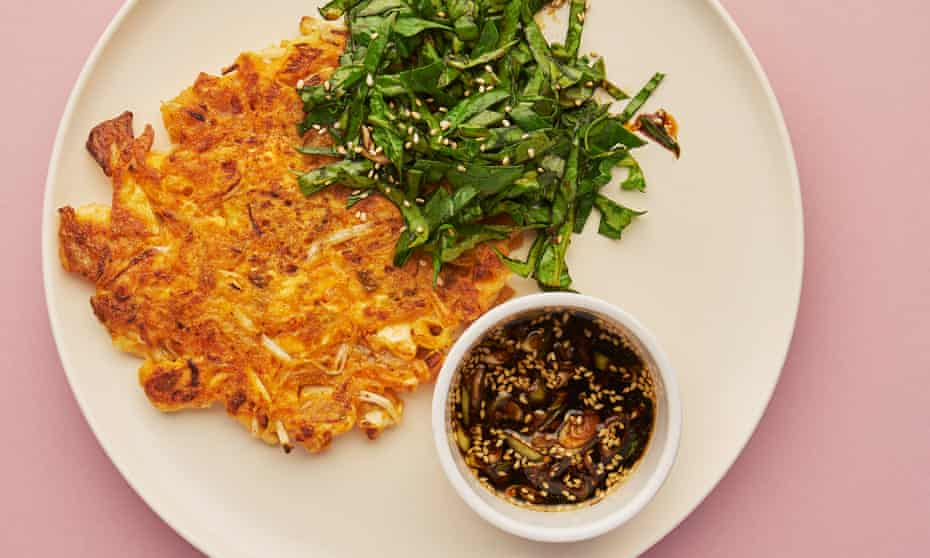
\includegraphics[width=10cm,height=10cm,keepaspectratio]{Recipe_Pictures/Kimchi_pancakes_with_spinach_salad.png}
\end{figure}
\emph{I discovered kimchi only a few months ago, but when I did, there were fireworks. I nearly ate a whole jar of Kim Kong Kimchi in a single salty, spicy and sour sitting. Then I went in search of recipes that would justify buying more, and became acquainted with the kimchi jeon at Oshibi, a Korean restaurant in York. A jeon is a forgiving pancake that absorbs tofu and most vegetables, but still becomes crisp, given enough time in the pan.\\ 
This makes four pancakes, or enough for a light lunch for four or dinner for two hungry people. The perennial problem with pancakes is how to keep them warm so everyone can eat together: once cooked, I keep mine in a warm spot and under foil.}\\\\ 
\textbf{Prep}: 10-15 min
\textbf{Cook}: 25 min
\textbf{Serves}: 2-4
\subsection*{Ingredients}
\begin{itemize}
\item 250g kimchi (suitable for vegans) 
\item 80g rice flour 
\item 80g plain flour
\item 1 tsp salt 
\item 200g (ie half a pack) drained firm tofu (such as Cauldron), cut into thin slivers
\item 80g bean sprouts (ie, one big handful)
\item 5 spring onions, trimmed and finely chopped
\end{itemize}

\begin{itemize}
\item 120g baby spinach leaves
\item Rapeseed oil
\item For the dipping sauce
\item 3 tbsp dark soy sauce
\item 2 tbsp toasted sesame oil
\item 1 $\frac{1}{4}$ tbsp rice vinegar
\item 2 tsp red chilli flakes
\item 1 tsp toasted sesame seeds, plus extra to garnish 
\end{itemize}

\subsection*{Steps}
\begin{enumerate}
\item Tip the kimchi into a sieve over a measuring jug, and press down to extract as much juice as possible. Measure the juice and, if need be, top it up to 200ml with tap water. Roughly chop the drained kimchi.
\item In a large bowl, use a fork to whisk the flours and salt, then stir in the kimchi juice. Add the kimchi, tofu, bean sprouts and spring onions – save a small handful of the onions for the sauce – and stir again. The batter should be wet but scoopable. Leave to stand for 10 minutes.
\item Meanwhile, make the sauce. In a small bowl, mix the soy, sesame oil, vinegar, chilli, the reserved spring onion and sesame seeds.
\item Finely shred the spinach, then put in a salad bowl, add two tablespoons of dipping sauce and toss to coat.
\item To cook the pancakes, heat half a tablespoon of oil in a medium frying pan (ideally nonstick) on a medium flame and swirl it around to coat the base of the pan. Pour in a quarter of the batter and spread it out with the back of a spoon until it’s 15cm in diameter. Cook for three to five minutes, until the bottom is crisp and golden, then flip and cook on the other side until that, too, is crisp and golden. Transfer to a warm place, cover with foil, and repeat with the remaining batter, adding a little extra oil to the pan for each pancake, if need be.
\item Serve warm with a big handful of spinach salad scattered on top and sprinkled with sesame seeds. Serve the sauce in little bowls on the side.
\end{enumerate}
\newpage

\section{Gujarati potato and cabbage curry}
\begin{figure}
\centering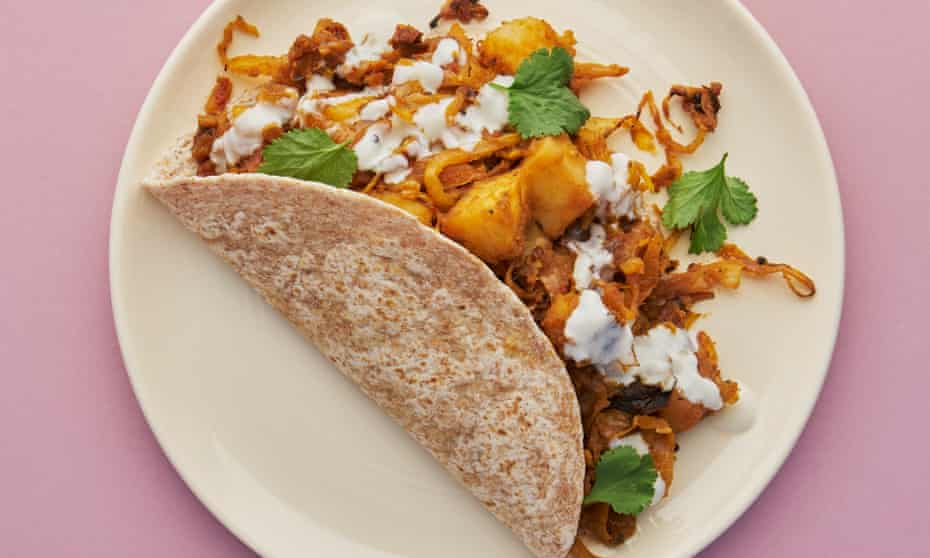
\includegraphics[width=10cm,height=10cm,keepaspectratio]{Recipe_Pictures/Gujarati_potato_and_cabbage_curry.png}
\end{figure}
\emph{Today’s recipe is an ancient dish that my ancestors cooked over wooden fires in their village on the Kathiawar peninsula in Gujarat, western India. It’s also something I ate regularly when I got home from school in Lincolnshire, while sitting in front of the telly and watching Neighbours, as well as something I wanted to eat almost every day when I was pregnant. It might be simple and cheap, but it’s also delicious and wholesome, and deserves to continue for many more generations.\\ 
My mother uses waxy potatoes such as charlotte or anya in this, because they hold their shape when cooked; I prefer crumbly, fudgy spuds such as maris pipers, which merge into the sauce. Boost the table offering with a dal or spinach curry.}\\\\ 
\textbf{Prep}: 10 min
\textbf{Cook}: 30 min
\textbf{Serves}: 4
\subsection*{Ingredients}
\begin{itemize}
\item 800g maris piper potatoes, peeled and cut into 2cm cubes
\item Salt and black pepper
\item 3 tbsp rapeseed oil
\item 1 pinch fenugreek seeds
\item $\frac{1}{4}$ tsp black mustard seeds
\item 1 tsp cumin seeds
\item 1 large onion, peeled and finely chopped
\item 4 garlic cloves, peeled and finely chopped
\item 200g tinned plum tomatoes with their juice (ie, half a tin)
\item 500g white cabbage (ie, half a large one), cored and shredded
\item 1 tsp ground coriander
\item $\frac{1}{3}$ tsp turmeric
\item 1 $\frac{1}{4}$ tsp ground red chilli powder
\item 250ml lukewarm water
\end{itemize}

\begin{itemize}
\item To serve
\item Chapatis
\item Non-dairy yoghurt
\item Fresh coriander
\end{itemize}

\subsection*{Steps}
\begin{enumerate}
\item Put the potatoes in a pan, cover with cold water, add a teaspoon of salt and bring to a boil. Cook until tender, then drain and leave to steam.
\item While the potatoes are cooking, heat the oil over a medium flame in a large frying pan for which you have a lid. Once it’s very hot, add the fenugreek, mustard and cumin seeds and, when they start to crackle, stir in the onion and fry for six minutes, until soft. Add the garlic, cook for two minutes, then add the tomatoes, tipping them in with one hand and crushing them with the other as they hit the pan. Cook until the tomatoes become concentrated and paste-like and the oil floats to the top – about eight to 10 minutes.
\item Turn up the heat, add the cabbage and stir until well coated in the tomato mixture, then cover the pan and leave to cook for about 10 minutes, stirring infrequently (every couple of minutes, say), so the cabbage caramelises a little while it softens.
\item When the cabbage is soft, fold in the potatoes, the ground spices and a teaspoon and a half of salt, and stir gently, so the potatoes don’t break up too much. Add the lukewarm water bit by bit, stirring after each addition, and leave to cook down for five minutes, until the liquid thickens into a sauce. Check and adjust the seasoning, then take off the heat.
\item Serve generous helpings of the curry with warm chapatis (heat according to the packet instructions) , a large spoonful of non-dairy yoghurt and a couple of sprigs of fresh coriander.
\end{enumerate}
\newpage

\chapter{March}
\section{Creamy butter bean gratin with roast tomatoes and salsa fresca}
\begin{figure}
\centering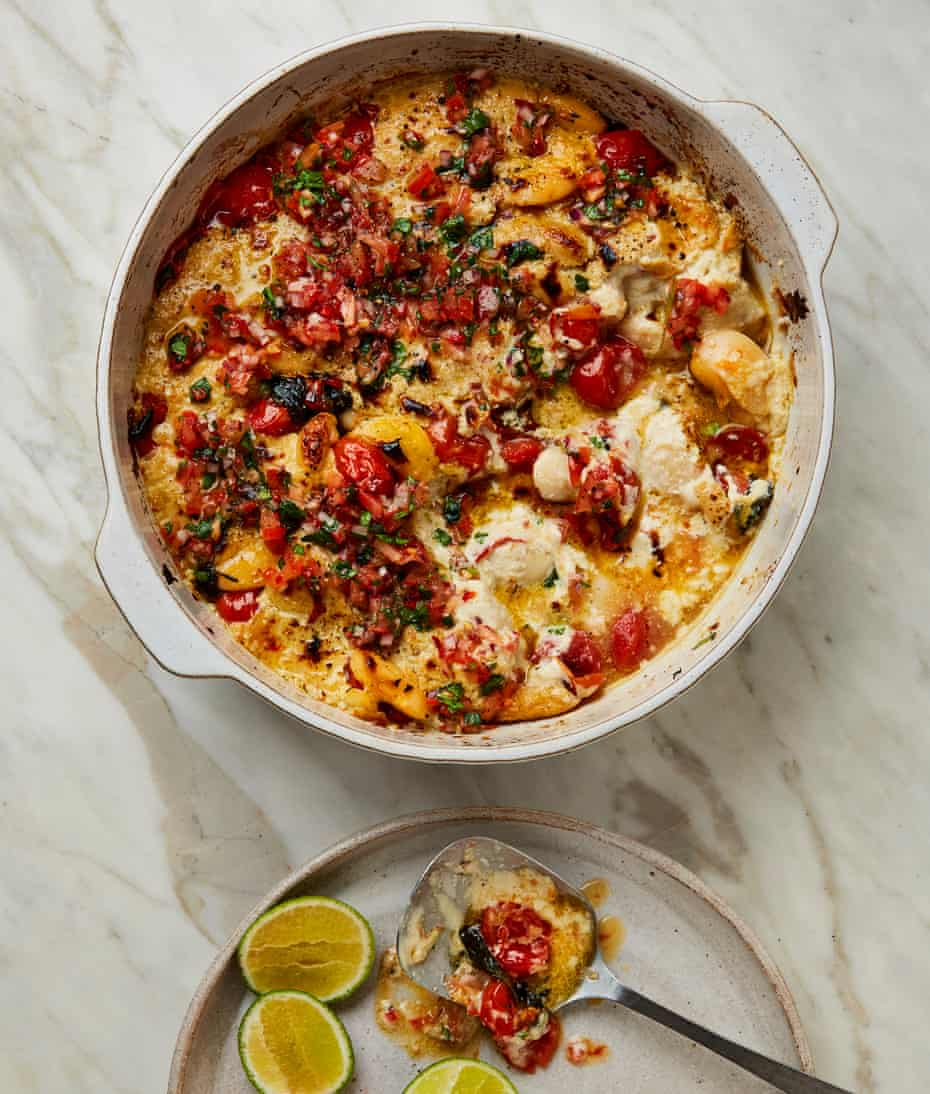
\includegraphics[width=10cm,height=10cm,keepaspectratio]{Recipe_Pictures/Creamy_butter_bean_gratin_with_roast_tomatoes_and_salsa_fresca.png}
\end{figure}
\emph{As promised, here’s another (completely different) use for the bechamel I introduced you to last week. This time, it’s flavoured with cumin and cooked in a gratin with butter beans and roast cherry tomatoes, with a zingy salsa fresca to cut through the richness. It’s pretty much a meal in one that needs only a salad or some sauteed greens by way of accompaniment. \\ 
Gnocchi would also work really well here instead of the beans; cook them in salted water before adding them to the roast tomatoes.}\\\\ 
\textbf{Prep}: 20 min
\textbf{Cook}: 50 min
\textbf{Serves}: 2-4
\subsection*{Ingredients}
\begin{itemize}
\item 450g sweet ripe cherry tomatoes, such as datterini
\item 15g coriander, leaves and soft stalks
\item 3 garlic cloves, peeled and crushed with the flat of a knife
\item 3$\frac{1}{4}$ tbsp olive oil
\item 2 tsp maple syrup 
\item 1 tsp flaked salt
\item Black pepper
\item 1 x 660g jar cooked butter beans, drained (425g net)
\end{itemize}

\begin{itemize}
\item For the cumin bechamel
\item 300g silken tofu, very well drained
\item 40g white miso paste
\item 2 tbsp olive oil
\item 2 tsp dried onion granules
\item 1 small garlic clove, peeled
\item $\frac{1}{4}$ tsp ground cumin
\item Lots of freshly grated nutmeg (or $\frac{1}{8}$ tsp ground nutmeg)
\item $\frac{1}{4}$ tsp fine salt
\end{itemize}

\begin{itemize}
\item For the salsa fresca
\item 1 medium ripe tomato, finely chopped (100g)
\item 1 red chilli, finely chopped (optional)
\item $\frac{1}{4}$ onion, finely chopped (30g)
\item 1$\frac{1}{4}$ tbsp good olive oil, plus extra to serve
\item 1 tbsp lime juice, plus lime wedges to serve
\item $\frac{1}{4}$ tsp fine salt
\item 5g (1$\frac{1}{3}$ tbsp) finely chopped coriander
\end{itemize}

\subsection*{Steps}
\begin{enumerate}
\item Heat the oven to 240C (220C fan)/475F/gas 9. Put the cherry tomatoes in a 26cm round ovenproof pan or baking dish in which they’ll all fit snugly in a single layer. Add the coriander, garlic, oil, maple syrup, salt and plenty of pepper, and stir to coat. Roast near the top of the oven for 25-30 minutes, until softened and slightly charred.
\item Meanwhile, put all the ingredients for the bechamel in a blender with about 10 twists of the pepper mill and blitz smooth.
\item Once the tomatoes are roasted, stir in the drained butter beans and a tablespoon of water. Turn the grill to its highest setting. Top the beans with the bechamel, leaving spaces here and there for the tomatoes and liquid to bubble through when grilled, then drizzle with oil and grill, again near the top of the oven, until golden brown and bubbling – depending on the strength of your grill, this will take anywhere between five and 12 minutes, so keep an eye on it. (If you have a blowtorch, use that to get a uniform char on the surface once the bechamel has heated through.) Remove and set aside to cool for five minutes.
\item Meanwhile, make the salsa fresca. In a small bowl, mix the tomato, chilli, onion, oil, lime juice and half a teaspoon of flaked salt. Just before serving, stir in the coriander.
\item Top the gratin with some of the salsa, then drizzle with oil, sprinkle with flaked salt and black pepper, and serve with lime wedges and the remaining salsa on the side.
\end{enumerate}
\newpage

\section{Curried caramelised onion galette}
\begin{figure}
\centering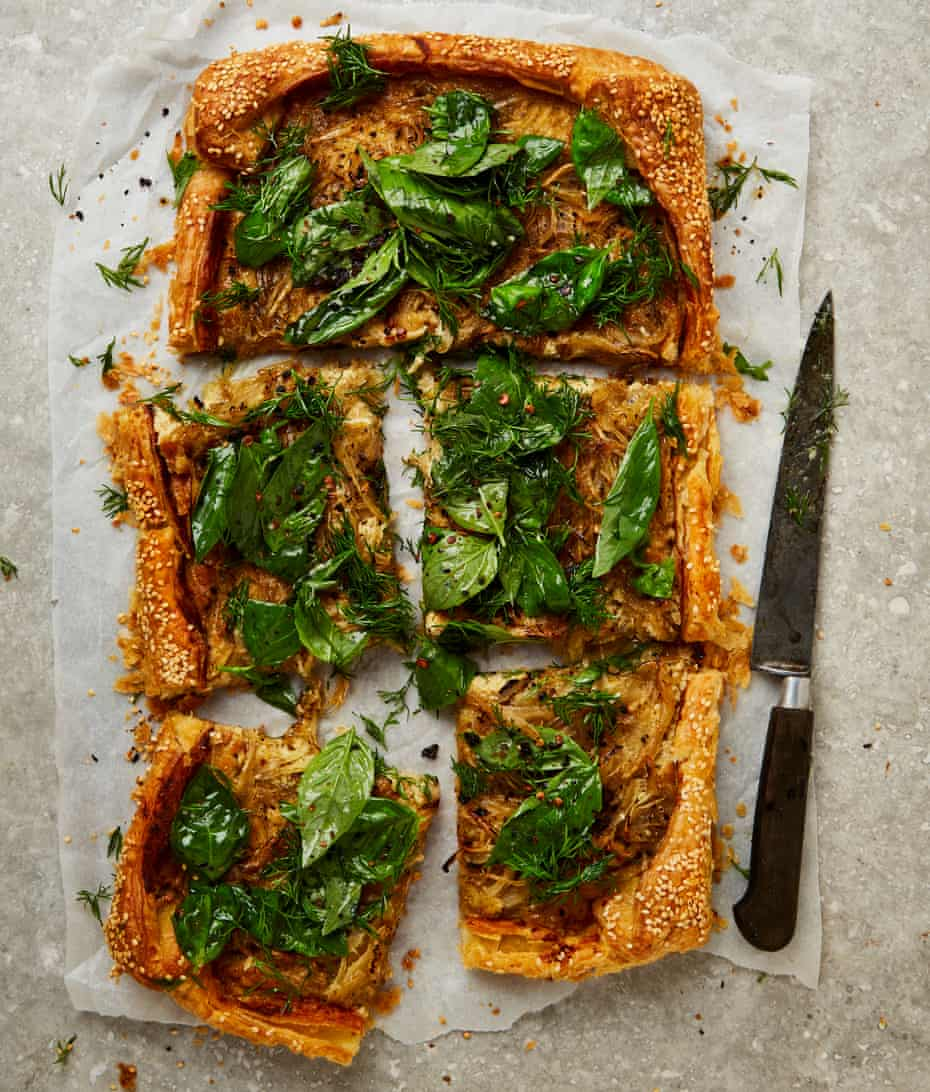
\includegraphics[width=10cm,height=10cm,keepaspectratio]{Recipe_Pictures/Curried_caramelised_onion_galette.png}
\end{figure}
\emph{The star of the show here is the bechamel – in a blind taste test, you’d never guess it was vegan. What’s more, it’s incredibly versatile. Here, I use it as the base for a galette topped with caramelised onions; you can also use it to make lasagne or cannelloni and moussaka (next week, I’ll show you another way to use it). Experiment with the flavour profile by subbing the curry powder for different spices or fresh herbs (which you can blend straight in), but I’d recommend keeping the nutmeg in the mix, because it lends the sauce a lovely, sweet nuttiness.}\\\\ 
\textbf{Prep}: 10 min
\textbf{Cook}: 1 hr 15 min
\textbf{Serves}: 2-4
\subsection*{Ingredients}
\begin{itemize}
\item 1 x ready-rolled puff pastry sheet, suitable for vegans (it usually comes in a 320g or 375g pack)
\item 2 medium onions, peeled and halved
\item 2$\frac{1}{4}$ tbsp maple syrup 
\item 2 tbsp olive oil, plus extra for brushing
\item $\frac{3}{4}$ tsp mild or medium curry powder
\item $\frac{1}{4}$ tsp fine salt
\item 1 tbsp sesame seeds
\item 1 big pinch flaked salt
\item 10g dill leaves
\item 10g basil leaves
\item 1 tsp lemon juice
\item Chipotle (or regular) chilli flakes, to serve
\end{itemize}

\begin{itemize}
\item For the curried bechamel
\item 300g silken tofu, very well drained
\item 40g white miso paste
\item 2 tbsp olive oil
\item 2 tsp dried onion granules
\item 1 small garlic clove, peeled and roughly chopped
\item $\frac{1}{4}$ tsp mild or medium curry powder
\item Lots of freshly grated nutmeg (or $\frac{1}{8}$ tsp ground nutmeg)
\item $\frac{1}{4}$ tsp fine salt 
\item Freshly ground black pepper (about 10 twists)
\end{itemize}

\subsection*{Steps}
\begin{enumerate}
\item Heat the oven to 220C (200C fan)/425F/gas 7. Unroll the pastry on to a large, flat baking tray. Put all the ingredients for the bechamel in a blender and blitz until completely smooth.
\item Very thinly slice the onion halves (use a mandoline, if you have one), then toss in a bowl with the maple syrup, olive oil, curry powder, fine salt and plenty of pepper and set aside.
\item Spoon the bechamel on to the pastry, then spread it out leaving a 3cm rim all around the edges. Spread out the onions on top of the bechamel.
\item Fold the rim of the pastry up and over the onions around the edges, then brush the exposed pastry with oil. Sprinkle the sesame seeds and flaked salt over the exposed pastry, pushing the seeds into the pastry so they stick.
\item Bake for 15 minutes, then remove the tray from the oven and turn down the temperature to 200C (180C fan)/390F/gas 6. The onions will at this stage have shrunk and clumped together a bit, so spread them out once again – this is to ensure they cook evenly. Drizzle with a little oil, return to the oven for 20-30 minutes, until the rim is puffed up and a deep, golden brown, then remove (keep an eye on it, just in case).
\item Turn the grill to its highest setting, then grill the top of the galette for a minute or two, or until the onions take on some more colour. Keep a very close eye on things, though, because you don’t want to burn the pastry; you just want to char the onions a little (if you have one, use a blowtorch to char the onions instead, because that will give you more control). Set aside to cool for 10 minutes.
\item Meanwhile, mix the herbs with the lemon juice, a drizzle of oil and a pinch of salt, arrange these over the top of the galette, sprinkle with chilli flakes and serve.
\end{enumerate}
\newpage

\section{Cassava, coconut and passion fruit cake}
\begin{figure}
\centering
\includegraphics[width=10cm,height=10cm,keepaspectratio]{Recipe_Pictures/Cassava,_coconut_and_passion_fruit_cake.png}
\end{figure}
\emph{My Brazilian mother always asks for this cake for her birthday – she loves the combination of cassava (or macaxeira, as we know it), coconut and passion fruit. I adore its unique texture; it’s caramelised and crisp on the outside and chewy and springy inside, a bit like mochi. It’s not overly sweet, either, which makes it the ideal mid-morning or afternoon treat with a cup of coffee. \\ 
The only time-consuming part of this recipe is peeling, grating and squeezing the cassava, after which all the ingredients come together very simply in a bowl. Alternatively, buy frozen grated cassava (available online and from many Asian supermarkets) to make the prep quicker.}\\\\ 
\textbf{Prep}: 15 min
\textbf{Cook}: 1 hr
\textbf{Rest}: 30 min
\textbf{Serves}: 6
\subsection*{Ingredients}
\begin{itemize}
\item 950g cassava roots (or 500g frozen grated cassava, defrosted)
\item 8 passion fruits
\item 100g plant butter, plus extra for greasing
\item 100g caster sugar, plus 2$\frac{1}{4}$ tbsp extra
\item 140g tinned coconut milk (at least 70\% coconut extract)
\item 100g condensed coconut milk
\item 50g desiccated coconut
\item 3 tbsp aquafaba (the liquid from a can of unsalted chickpeas or white beans)
\item 2 tsp tangerine zest (from 2 tangerines), or orange zest 
\item 1$\frac{1}{4}$ tsp lime zest (from 2 limes)
\item 1 tsp vanilla bean paste
\item $\frac{1}{8}$ tsp fine salt
\item Flaked salt, to serve
\end{itemize}

\subsection*{Steps}
\begin{enumerate}
\item Heat the oven to 220C (200C fan)/425F/gas 7. Peel the cassava roots, removing the thick, brown skin as well as the pinkish layer beneath it, and don’t use any part of the cassava that’s black or soft. Finely grate the cassava on the smaller holes of a box grater (you should get 600g), then transfer the flesh to a colander and put it in the sink. Squeeze the cassava vigorously, to get ridof as much liquid as possible (you should end up with 500g), then transfer to a large bowl.
\item Halve the passion fruits and scoop the flesh and seeds into a sieve set over the bowl of cassava. Push down on it with the back of a spoon to extract all the juice, then discard the seeds and pulp.
\item Thoroughly grease a 20cm nonstick cake tin without a removable base with plenty of butter, making sure the inside is completely covered. Scatter one and a half tablespoons of sugar into the tin, and shake to ensure it covers the greased sides and base. (If your tin isn’t nonstick, line the base first with a circle of nonstick parchment paper, then continue with the butter and sugar.)
\item Melt 100g butter over a low heat until warm and liquid. Add this, 100g sugar, the coconut milk, condensed coconut milk, desiccated coconut, aquafaba, tangerine zest, lime zest, vanilla and an eighth of a teaspoon of fine salt to the cassava bowl, then mix thoroughly.
\item Spoon the cassava mixture into the greased and sugared tin, level out the surface, then evenly sprinkle the remaining tablespoon of sugar over the top. Bake for 55 minutes, turning the tin once halfway, until the top is crisp and golden brown. Leave to cool for five minutes, then run a knife around the edge of the cake to release it from the tin. Put a rack over the tin, then flip the cake out on to it. The cake should end up on the rack, but, if not, gently release it from the bottom of the tin with a palette knife or spatula. Leave to cool and set for at least 30 minutes (this is very important!), then sprinkle with flaked salt and enjoy with coffee.
\end{enumerate}
\newpage

\section{Tomato and blood orange salad with ginger tahini sauce}
\begin{figure}
\centering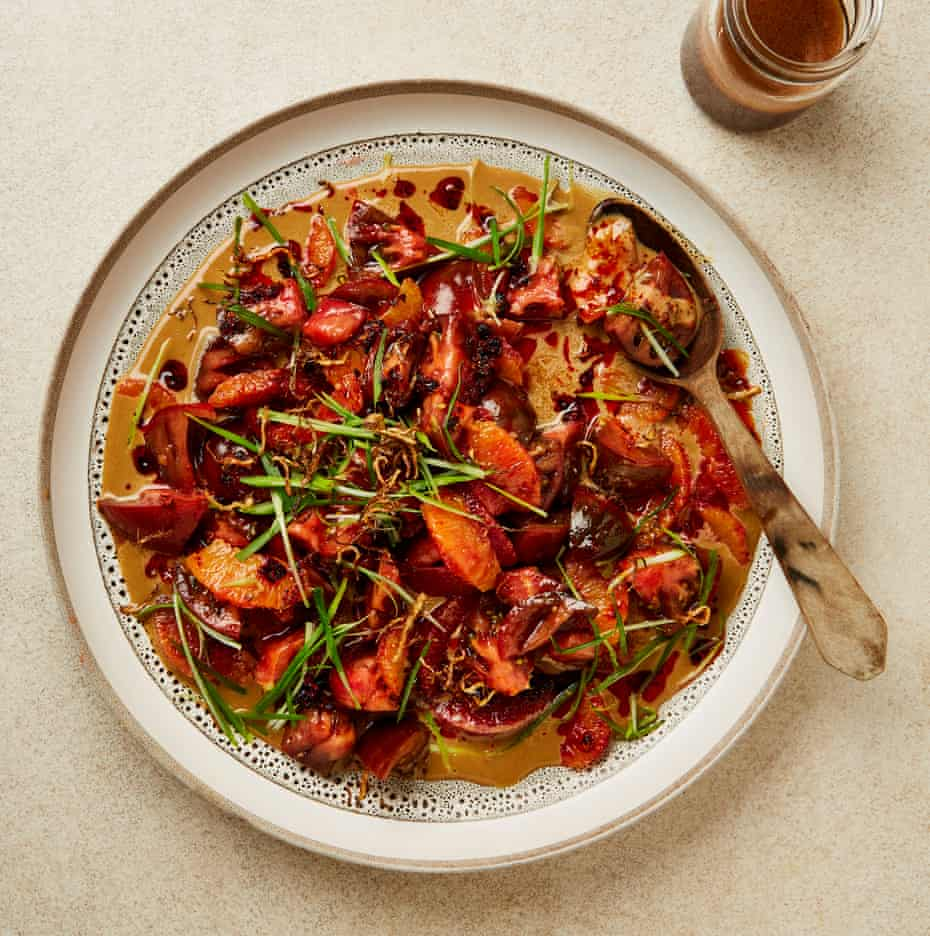
\includegraphics[width=10cm,height=10cm,keepaspectratio]{Recipe_Pictures/Tomato_and_blood_orange_salad_with_ginger_tahini_sauce.png}
\end{figure}
\emph{I first developed this recipe for a pop-up at the brilliant Supa Ya Ramen in London in late January. That week, blood oranges and iberiko winter tomatoes were glimmering on the shelves of my local grocer and I just knew I had to create something with them. What with the unpredictability of the seasons these days, I don’t know if blood oranges and iberiko tomatoes will still be singing quite as heartily whenyou read this, but you can always use regular oranges or tangerines instead of the blood oranges and any ripe, sweet tomato you can get your hands on.}\\\\ 
\textbf{Prep}: 15 min
\textbf{Cook}: 5 min
\textbf{Serves}: 4
\subsection*{Ingredients}
\begin{itemize}
\item 500g ripe winter tomatoes (I used iberiko tomatoes)
\item Salt
\item 3 blood oranges (or 2 regular oranges)
\item 3 spring onions, green ends julienned (save the rest for another dish)
\item Chiu chow or crispy chilli oil, to serve (optional)
\end{itemize}

\begin{itemize}
\item For the dressing
\item 4 tbsp light olive oil
\item 40g fresh ginger, peeled and julienned
\item 2 tbsp soy sauce or tamari 
\item 1 tbsp lime juice
\item 1 small garlic clove, finely grated/crushed
\item $\frac{1}{4}$ tbsp maple syrup
\item $\frac{1}{4}$ tsp toasted sesame oil
\end{itemize}

\begin{itemize}
\item For the tahini sauce
\item 60g tahini 
\item 2 tbsp maple syrup
\item 2 tbsp soy sauce
\item 1 tbsp lime juice
\item 1 tsp very finely grated fresh ginger
\end{itemize}

\subsection*{Steps}
\begin{enumerate}
\item For the dressing, put the oil and one stick of the ginger in a medium saucepan set over a medium-low heat. Once it starts to sizzle, add the rest of the ginger and fry gently, stirring often with a fork to separate the pieces, until the ginger is a light golden brown – this should take about three and a half minutes, but keep a close eye on it because the ginger can quite quickly turn from golden to brown and burnt. Strain the crisped ginger through a sieve, collecting the oil in a bowl underneath. Spread out the ginger on a plate, sprinkle with salt and set aside.
\item Put the soy sauce, lime juice, garlic, maple syrup and sesame oil in a large bowl with two tablespoons of the ginger frying oil. Cut the tomatoes into random, bite-sized pieces and add to the bowl. Add a pinch of salt, gently mix and set aside to marinate.
\item Put all the ingredients for the tahini ginger sauce in a medium bowl, add a tablespoon of water and whisk vigorously until completely smooth.
\item Cut the tops and bottoms off the oranges. Using a sharp knife, remove the skin and white pith, then cut between the individual membranes to release the segments. Add any juice to the tomato bowl and set aside the segments.
\item Spoon the tahini sauce on to a lipped platter. Top with the tomatoes, using your hands as a natural sieve so you don’t take all the dressing with you. Arrange the blood orange segments evenly among the tomatoes. Drizzle over some chilli oil, finish with the spring onions and crisp ginger, and serve with the remaining dressing on the side.
\item  Ixta Belfrage’s debut solo cookbook, Mezcla: Recipes to Excite, is published by Ebury in summer 2022. Meera Sodha is away.
\end{enumerate}
\newpage

\section{Oat, spice and currant cookies}
\begin{figure}
\centering
\includegraphics[width=10cm,height=10cm,keepaspectratio]{Recipe_Pictures/Oat,_spice_and_currant_cookies.png}
\end{figure}
\emph{In the corner of the kitchen of the house I grew up in was a strawberry-shaped biscuit jar. Being offered a biscuit was always a thrill, but I wasn’t tall enough to see inside, so I’d stand on a stool, reach in and feel around for a favourite. Back then, I wasn’t keen on smooth ones (digestives), and was especially partial to those sandwiched with cream (two for one!), but the holy grail were the ones that mum sometimes made herself: oat cookies. They, like today’s recipe, were craggy and crisp outside, chewy inside, studded with currants and flavoured with chai masala.\\ 
These make a welcome, chocolate-free Easter treat.}\\\\ 
\textbf{Prep}: 5 min
\textbf{Cook}: 25 min
\textbf{Makes}: 16
\subsection*{Ingredients}
\begin{itemize}
\item 180g wholegrain spelt flour 
\item 50g rolled porridge oats 
\item 1 tsp baking powder 
\item $\frac{1}{4}$ tsp bicarbonate of soda 
\item $\frac{1}{4}$ tsp flaky sea salt, crumbled 
\item 100g currants 
\item 2 tsp chai or mixed spice
\item 50g dark brown soft sugar 
\item 100g golden syrup
\item 120ml cold-pressed rapeseed oil
\end{itemize}

\subsection*{Steps}
\begin{enumerate}
\item Heat the oven to 200C (180C fan)/390F/gas 6 and line a couple of large trays with baking paper.
\item In a heatproof bowl, combine the spelt flour, rolled oats, baking powder, bicarb, sea salt, currants and chai spice, and whisk to mix well.
\item Put the sugar, syrup and oil in a small saucepan, set it over a low heat, cook until the mixture comes to a boil, then take off the heat. Pour into the bowl of dry ingredients and stir with a wooden spoon until everything comes together into a dough.
\item Roll into balls the size of a ping-pong ball and weighing about 40g each, and place on the baking sheets spaced about 10cm apart – there’s no need to flatten them. Bake for 12 minutes, or until golden in the centre and starting to crisp to a golden brown at the edges.
\item Remove and leave to cool on the sheets – these cookies regain their integrity when they cool, so they need a bit of a rest before eating.
\end{enumerate}
\newpage

\section{Swede and mushroom tacos with peanut salsa}
\begin{figure}
\centering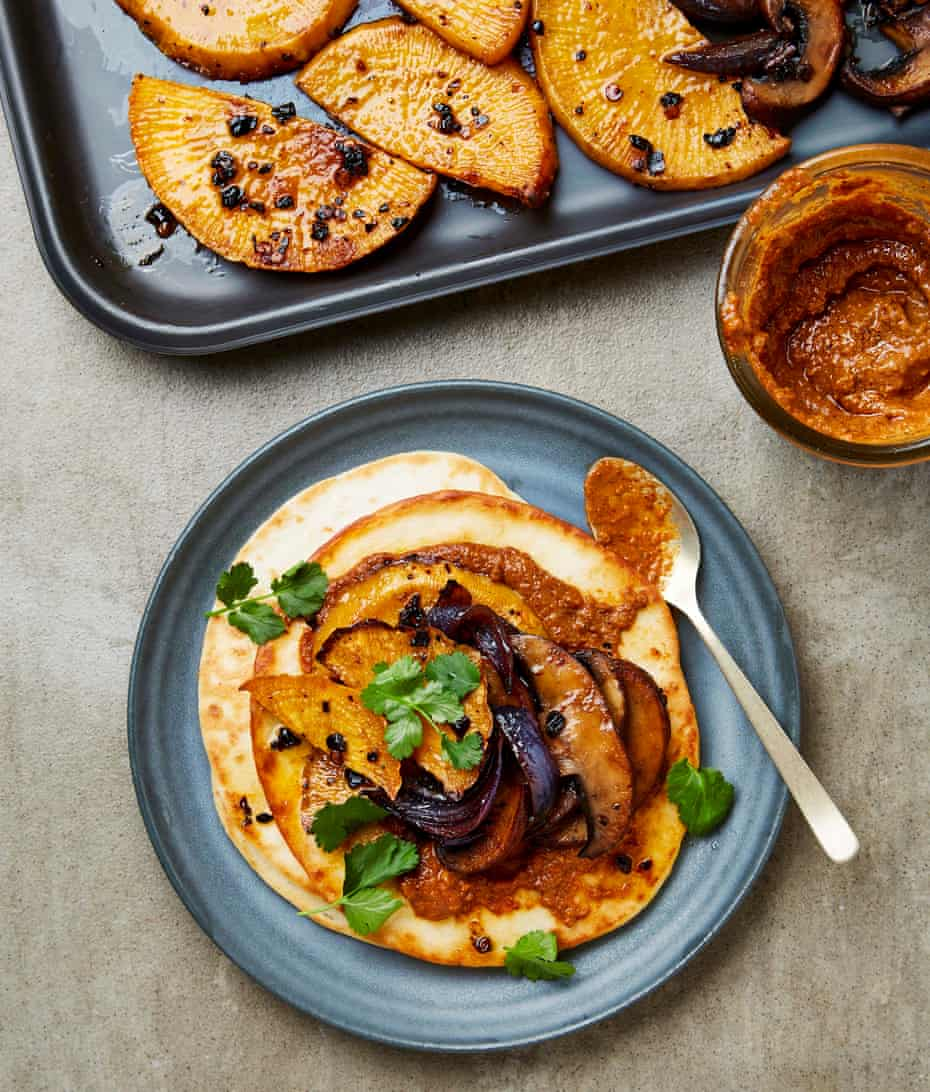
\includegraphics[width=10cm,height=10cm,keepaspectratio]{Recipe_Pictures/Swede_and_mushroom_tacos_with_peanut_salsa.png}
\end{figure}
\emph{I’m very fond of the swede. It has a bit of the Cinderella narrative about it: often cast aside and underappreciated, but, when given attention and love, it blossoms – in this particular story, into a delicious dinner. It’s such a star, you can cook it in any way there is to cook an ingredient, but roasting is my favourite approach. Then it becomes buttery and fondant-like, and in today’s recipe sits pretty among mushrooms, spice and peanut salsa.}\\\\ 
\textbf{Prep}: 15 min
\textbf{Cook}: 45 min
\textbf{Serves}: 4
\subsection*{Ingredients}
\begin{itemize}
\item Rapeseed oil
\item 1 tbsp ancho flakes
\item $\frac{1}{4}$ tsp ground cloves
\item $\frac{1}{4}$ tsp ground cumin
\item 1 tbsp chipotle flakes
\item Fine sea salt
\item 1 swede (about 800g), peeled, cut in half and then into 1cm slices
\item 1 red onion, peeled and cut into 1$\frac{1}{4}$cm wedges
\item 300g portobello mushrooms, cut into 1cm slices
\item 5 fat garlic cloves, peeled and halved
\item 100g salted roasted peanuts
\item 2$\frac{1}{4}$ tsp cider vinegar
\item Tortillas (flour or corn), to serve 
\item A few coriander leaves, chopped, to serve (optional) 
\end{itemize}

\subsection*{Steps}
\begin{enumerate}
\item Heat the oven to 220C (200C fan)/425F/gas 7. First, make the dressing: put five tablespoons of oil, the ancho flakes, cloves, cumin, half a tablespoon of chipotle flakes and a teaspoon of salt into a small bowl, and stir to combine.
\item In a large bowl, mix the swede with half of the spiced oil, toss with your hands to coat, then tip out on to an oven tray. In the same large bowl, mix the onion, mushrooms and the rest of the spiced oil, toss and tip out on to a second oven tray. Space out all the vegetables so they’re not on top of each other. Bake the mushrooms and onions for 20 minutes and the swede for 30 minutes, until all the vegetables are soft and starting to caramelise.
\item While the vegetables are roasting, make the salsa. Put 75ml rapeseed oil in a small saucepan with the garlic halves and peanuts, set over a low heat and bring slowly to a boil. Turn down the heat to a simmer and cook for four to five minutes, or until the garlic starts to colour. Take off the heat, add half a tablespoon of chipotle flakes and a quarter-teaspoon of salt, and set aside to cool. Once cooled, add the vinegar and seven tablespoons (105ml) of water, then blitz with a stick blender until the salsa is the consistency of custard.
\item To serve, heat up the tortillas (I pan-fry mine), top each with a dollop of the salsa, top that with some swede and then with mushrooms and onions, scatter with coriander leaves, if using, and devour.
\end{enumerate}
\newpage

\section{Aubergine donburi}
\begin{figure}
\centering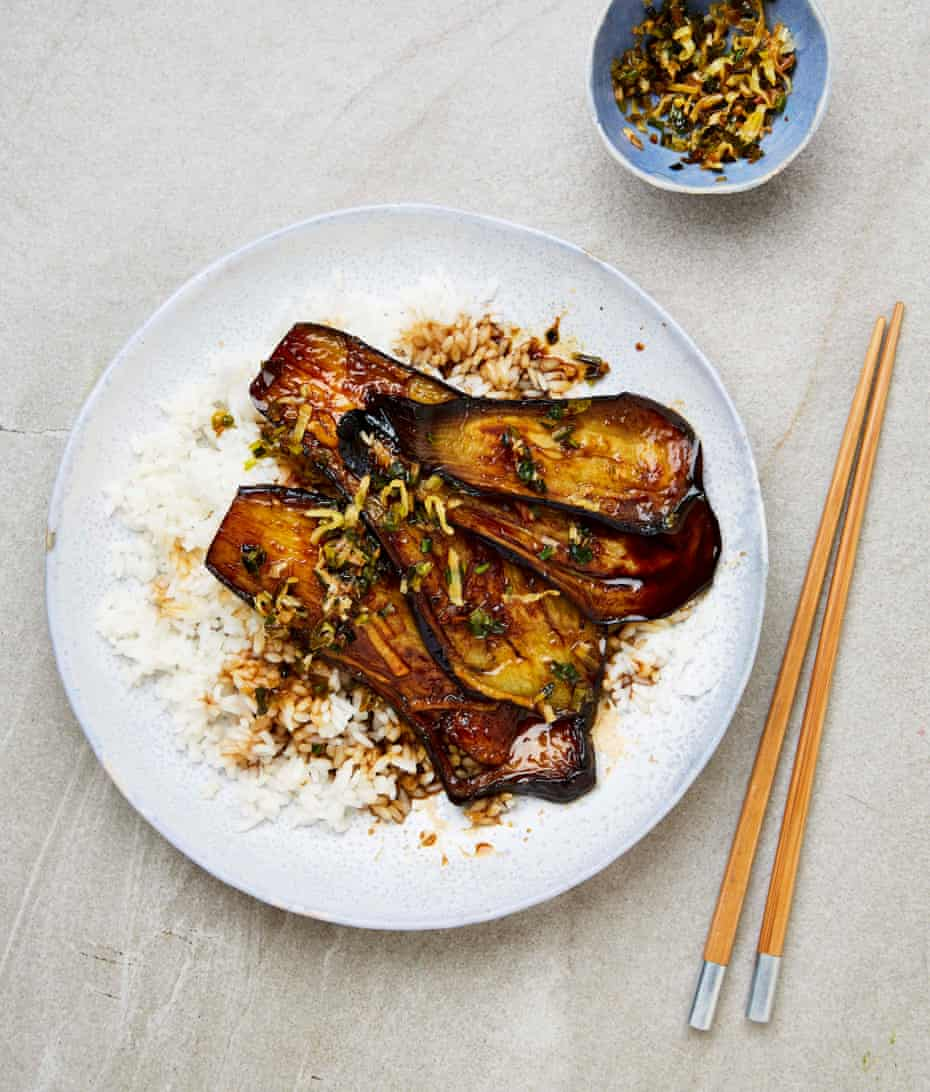
\includegraphics[width=10cm,height=10cm,keepaspectratio]{Recipe_Pictures/Aubergine_donburi.png}
\end{figure}
\emph{What I love about donburi, or Japanese rice bowls, is that they are complete meals in themselves. The rice is built in as part of the equation from the very start, rather than merely as a serving suggestion. This means, I think, that the sweet sauce in which these aubergines are simmered is designed specifically with the rice in mind. It is reduced until sticky enough to glaze the aubergines and potent enough that it needs to lean on rice to provide a respite from the intensity of flavour. It’s simple, but perfect.\\ 
I’ve taken the liberty of using one of my favourite toppings – fried and salted spring onions and ginger doused in a little vinegar – but if you don’t have time to make it, use thinly match-sticked fresh ginger or sliced spring onions instead.}\\\\ 
\textbf{Prep}: 10 min
\textbf{Cook}: 1 hr 10 min
\textbf{Serves}: 4
\subsection*{Ingredients}
\begin{itemize}
\item For the aubergines
\item 350g short-grain rice
\item 4 tbsp cooking sake
\item 4 tbsp light soy sauce
\item 2$\frac{1}{4}$ tbsp mirin
\item 2 garlic cloves, peeled and crushed
\item 3 aubergines, cut lengthways into 1cm slices
\item Rapeseed oil, for frying
\end{itemize}

\begin{itemize}
\item For the fried ginger and onions
\item 3 tbsp rapeseed oil
\item 50g ginger, peeled and cut into fine matchsticks
\item 6 spring onions, trimmed and finely chopped
\item $\frac{1}{4}$ tsp fine sea salt
\item 2 tsp white-wine vinegar
\end{itemize}

\subsection*{Steps}
\begin{enumerate}
\item Wash the rice in a sieve until the water runs clear, then transfer to a saucepan for which you have a lid. Cover with warm water, soak for five minutes, then drain, cover with 400ml cold water and bring to a boil. Turn down the heat to a whisper, cook for 12 minutes, then take the pan off the heat and put to one side, still covered.
\item Meanwhile, make the donburi sauce. In a small bowl, mix the sake, soy sauce, mirin, garlic and a pinch of the match-sticked ginger from the dressing.
\item Line a plate or board with kitchen paper. Heat three tablespoons of oil in a wide frying pan over a medium heat, add the remaining ginger and spring onions, and cook for about eight minutes, until soft and beginning to caramelise. Tip into a bowl, stir in the salt and vinegar, and set aside.
\item Put a little more oil in the frying pan, then, cooking them in batches, lay in the aubergine slices side by side and fry for three minutes, or until golden brown. Turn over and fry on the other side until tender and golden brown, then transfer to the lined plate to drain and repeat with the remaining aubergine slices, adding more oil as required.
\item Once all the aubergines are fried, gently return them all to the pan in layers and turn down the heat. Pour the donburi sauce over the top, leave it to bubble for a couple of minutes, until reduced and sticky, then take off the heat. (If the sauce threatens to vanish altogether, add a little water to rehydrate – you want this a bit saucy.)
\item Distribute the hot rice between four plates, lay slices of aubergine on top and spoon over a little sauce. Add a scattering of the fried salted ginger and spring onion, and serve.
\end{enumerate}
\newpage

\section{Whole broccoli and zhoug spaghetti}
\begin{figure}
\centering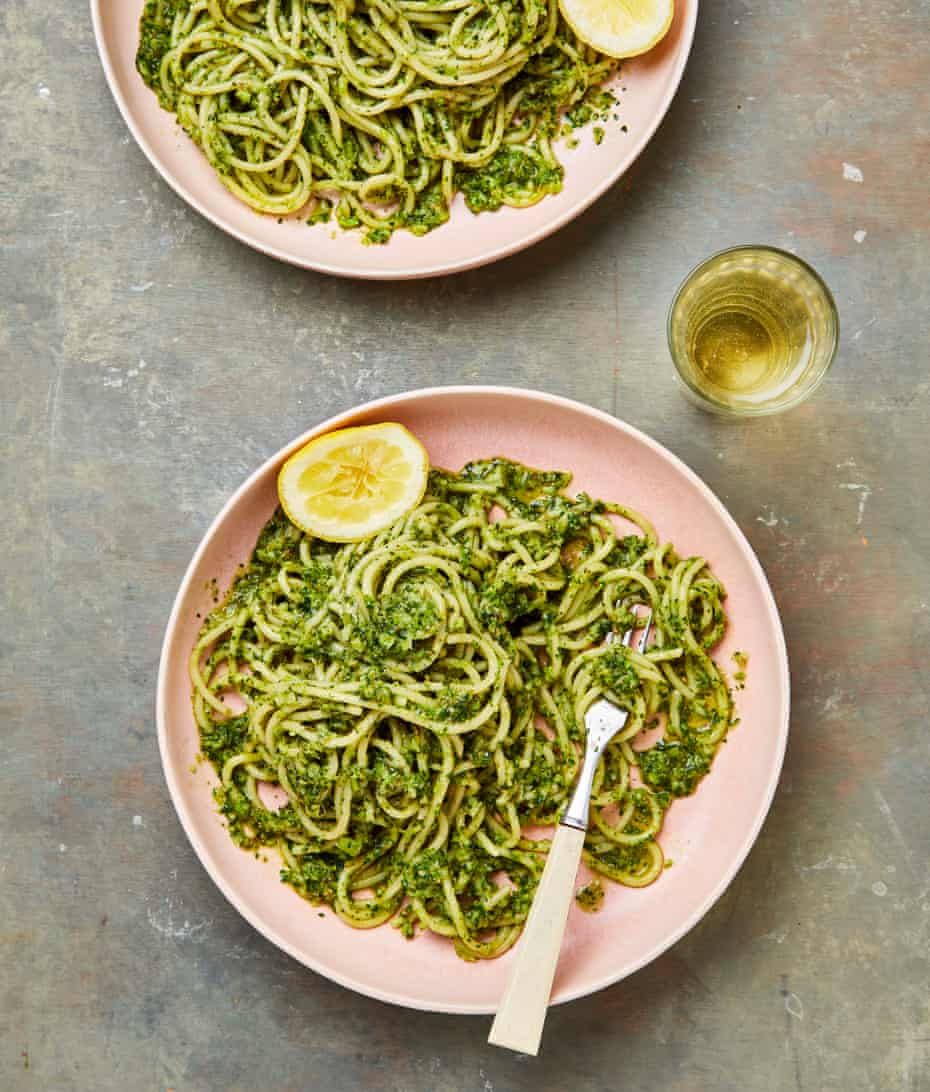
\includegraphics[width=10cm,height=10cm,keepaspectratio]{Recipe_Pictures/Whole_broccoli_and_zhoug_spaghetti.png}
\end{figure}
\emph{I could write a (short) cookbook on how to incorporate a whole head of broccoli into a meal. It’s the one vegetable that is a failsafe start to any dinner in my house, because it’s guaranteed to be in the fridge and eaten by all the family. In this recipe, the broccoli and spaghetti provide a soft backdrop to zhoug, an addictive and eye-openingly brilliant paste that’s popular across the Middle East. I’ve used fresh coriander, cumin, cardamom, but I dare say you could treat this recipe as more of a guide than a set of rules, and use whatever herbs and spices you have to hand.\\ 
You’ll need a food processor to make this.}\\\\ 
\textbf{Prep}: 10 min
\textbf{Cook}: 40 min
\textbf{Serves}: 4
\subsection*{Ingredients}
\begin{itemize}
\item 1 whole head broccoli (about 350g)
\item 60g fresh coriander, roughly chopped
\item 30g fresh flat-leaf parsley, roughly chopped
\item 3 green jalapeños, deseeded and finely chopped
\item 1$\frac{1}{4}$ tsp ground cumin
\item 1$\frac{1}{4}$ tsp ground coriander
\item $\frac{1}{4}$ tsp ground cardamom
\item 1$\frac{1}{4}$ tbsp lemon juice
\item 5 tbsp extra-virgin olive oil, plus 2 tbsp extra for frying
\item Salt 
\item 300g spaghetti
\end{itemize}

\subsection*{Steps}
\begin{enumerate}
\item Chop off and discard any woody bits from the broccoli stem, then roughly chop the whole head into pieces, blitz to a mince in a food processor and scrape into a large bowl.
\item Next, make the zhoug. Put the fresh coriander, parsley, chillies, cumin, ground coriander, cardamom, lemon juice, five tablespoons of oil and half a teaspoon of salt into the food processor and blitz to a smooth paste.
\item In a large nonstick frying pan, heat the remaining two tablespoons of oil over a medium heat and, when hot, add the blitzed broccoli and a half-teaspoon of salt. Cook, stirring every now and then, for about 10 minutes, until sweet and soft, then turn off the heat.
\item Cook the spaghetti in salted boiling water until al dente and, while it’s cooking, carefully dip a mug into the pot and collect a mugful of the hot pasta water.
\item Drain the pasta, tip into the broccoli pan, add the zhoug and toss to combine. Add some of the reserved pasta cooking water to loosen it – I used about eight tablespoons – until it looks nice and saucy. Check for seasoning, adjusting the salt, chilli or lemon as you wish, then serve on plates or bowls and eat hot.
\end{enumerate}
\newpage

\section{Portobello mushroom and hoisin sauce pancakes}
\begin{figure}
\centering\includegraphics[width=10cm,height=10cm,keepaspectratio]{Recipe_Pictures/Portobello_mushroom_and_hoisin_sauce_pancakes.png}
\end{figure}
\emph{Hoisin sauce marked many a childhood Chinese restaurant trip. Until, one day at the school gates, Mum accosted Mrs Pang, an excellent cook and the mother of a schoolfriend, and asked how she could make it at home. Mrs Pang introduced Mum to a tinned sauce available at our local Asian supermarket, and there began at home what is known as ‘The Time of Hoisin’, where we ate the stuff on or with everything, including mushrooms.\\ 
Although you can still buy the tinned sauce, it is very sweet, and besides, it’s much more satisfying to whip up this approximation in a matter of minutes.\\ 
You will need to source fermented or salted black beans for this recipe – a worthwhile endeavour, because you can use them in my recipes for mapo tofu or burnt garlic and black bean noodles. You should be able to find them in your local Chinese shop or online. You’ll also need two large baking trays – mine are around 40cm x 30cm.}\\\\ 
\textbf{Prep}: 15 min
\textbf{Cook}: 25 min
\textbf{Serves}: 4 as part of a larger meal
\subsection*{Ingredients}
\begin{itemize}
\item 8 spring onions
\item $\frac{1}{4}$ cucumber
\item 12 large portobello mushrooms (1.2kg), cleaned and cut into 1cm slices, or brown or shiitake mushrooms
\item 4 tbsp toasted sesame oil
\item 1$\frac{1}{4}$ tsp Chinese five spice
\item 4 tbsp smooth peanut butter
\item 2$\frac{1}{4}$ tbsp brown rice syrup, or 1 tbsp light molasses/agave syrup, or brown sugar
\item 1$\frac{1}{4}$ tbsp rice-wine vinegar
\item 3 tbsp light soy sauce
\item 2 tsp salted fermented black beans, crushed in 4 tsp water, or jarred black bean paste
\item 12 Chinese-style pancakes (they’re only flour and water, and not hard to make at home)
\item Vegan mayonnaise, to serve
\end{itemize}

\subsection*{Steps}
\begin{enumerate}
\item Heat the oven to 220C (200C fan)/425F/gas 7. Lay the spring onions on a chopping board horizontally, cut in half, then shred into long, thin strips. Halve the cucumber, scrape out the seeds with a teaspoon and discard, then cut the cucumber into the same length and width as the spring onions.
\item Put the sliced mushrooms in a large bowl, toss in the sesame oil, distribute evenly across two big baking trays (there will be some overlap) and roast for 20 minutes.
\item Meanwhile, whisk the five spice, peanut butter, rice syrup, vinegar, soy and black beans to make the hoisin sauce.
\item After the mushrooms have been cooking for 20 minutes, put them all on one of the two baking trays, pour over the hoisin sauce, toss to coat, and return to the oven for five minutes, just so the sauce heats through and goes sticky. Meanwhile, warm the pancakes according to the packet instructions.
\item To serve, spread a warm pancake with a little mayonnaise, top with some mushrooms, a few slices of spring onion and cucumber, roll up tight and eat.
\end{enumerate}
\newpage

\section{Butternut squash and sweetcorn erriseri}
\begin{figure}
\centering\includegraphics[width=10cm,height=10cm,keepaspectratio]{Recipe_Pictures/Butternut_squash_and_sweetcorn_erriseri.png}
\end{figure}
\emph{In Mumbai, up to 200,000 dabbas, or containers of home-cooked food, are delivered from people’s homes to workplaces every day by dabbawalas, who travel on foot or by bike. It’s an epic story of India’s love of home cooking, and of sustainability. \\ 
Now, thanks to Anshu Ahuja and her company, Dabba Drop, Londoners can eat her Indian home cooking delivered by bike. This erriseri – a sweet, rich and sour stew – is a go-to recipe for Anshu’s family: it’s what her grandmother used to make for Sunday lunch, it’s what her mother makes if guests turn up and it’s what Anshu now makes for friends and family.\\ 
There might seem to be a lot of chillies in this, but it’s not a hot dish, because the natural sweetness of the squash and sweetcorn, combined with the rich coconut milk and spiky lime, balance things out. Fresh curry leaves are now sold in most major supermarkets.}\\\\ 
\textbf{Prep}: 10 min
\textbf{Cook}: 45 min
\textbf{Serves}: 4
\subsection*{Ingredients}
\begin{itemize}
\item 1 butternut squash (1kg), washed
\item Sunflower oil – I like Mr Organic
\item Fine sea salt
\item 1 x 340g tin sweetcorn, drained
\item 2 tsp black mustard seeds
\item 12 curry leaves
\item 1 large onion, peeled and finely chopped
\item 4 garlic cloves, peeled and minced
\item 3 green finger chillies, finely chopped
\item 2 tsp turmeric
\item 1 x 400ml tin coconut milk
\item 2 tbsp fresh lemon juice (ie, from 1 lemon)
\item Coriander leaves, to garnish
\end{itemize}

\subsection*{Steps}
\begin{enumerate}
\item Cut the squash in half (no need to peel), scoop out and discard the seeds, then cut it into 2cm cubes. Heat the oven to 200C (180C fan)/gas 6. Tip the squash pieces on to an oven tray, pour over two tablespoons of oil and a good sprinkling of salt, and toss to coat. Bake for 25-30 minutes, until the squash chunks are tender and their edges caramelised.
\item Add two tablespoons of water to the drained sweetcorn kernels and blend to a smooth paste (I use a stick blender).
\item In a large frying pan, heat two tablespoons of oil and, when hot, add the mustard seeds and curry leaves, and leave them to crackle and pop for a minute. Now add the onion and cook, stirring occasionally, for about 10 minutes, until translucent and turning golden, then add the garlic and chillies, and cook for two minutes. Stir in the sweetcorn paste, turmeric and a teaspoon and a half of salt, cook for a minute, then add the coconut milk (keep the tin) and whisk so everything is combined and the curry sauce is a vibrant yellow.
\item Half-fill the coconut milk tin with water and add to the pot to loosen the curry – you may need a little more or less water than this, depending on the thickness of your coconut milk – bring to a boil and simmer for five minutes, until it starts to thicken. Stir in the roast squash and lemon juice, and check the seasoning. Garnish with coriander and serve immediately.
\end{enumerate}
\newpage

\section{Polenta with balsamic fried radicchio, mushrooms and sage}
\begin{figure}
\centering\includegraphics[width=10cm,height=10cm,keepaspectratio]{Recipe_Pictures/Polenta_with_balsamic_fried_radicchio,_mushrooms_and_sage.png}
\end{figure}
\emph{Radicchio, in its many varieties and hues of pink, is nature’s most outrageous flirt. \\ 
The castelfranco is big and blowsy, like a giant rose that’s almost too good to eat. The trevisano is torpedo-shaped, contained and very secretive. The most commonly available here, chioggia, looks like red cabbage except for its white veins like snow-covered trees. And tardivo has tendrils like Medusa’s hair that stay robust and firm when cooked. \\ 
Whichever type you find (and you can use any in this dish), they all have a very special bitterness that makes them a perfect partner for sweet-and-sour balsamic vinegar and the earthy richness of mushrooms and polenta.\\ 
Once, these special leaves were the preserve of upmarket Italian restaurants only, but these days they make regular cameos in farmers’ markets and even some supermarkets. If you can’t find them, use red endive (chicory) instead, but because bitterness varies between the different breeds, so add the agave syrup to taste.}\\\\ 
\textbf{Prep}: 15 min
\textbf{Cook}: 45 min
\textbf{Serves}: 4
\subsection*{Ingredients}
\begin{itemize}
\item 1 litre vegetable stock
\item 180g instant polenta
\item Fine sea salt
\item Olive oil, for cooking
\item 1 large head radicchio tardivo (around 500g), cut into 1cm shreds
\item Balsamic vinegar
\item 2 tbsp agave syrup (or to taste)
\item 1 tbsp lemon juice
\item 12 sage leaves
\item 500g chestnut mushrooms, sliced
\item 4 garlic cloves, peeled and minced
\item Extra-virgin olive oil, to finish
\end{itemize}

\subsection*{Steps}
\begin{enumerate}
\item Put the stock in a saucepan for which you have a lid and bring it to a rolling boil. Pour in the polenta in a thin, steady stream, whisking as you do so, then keep whisking for another minute. The polenta will quickly thicken to a paste, and the moment it starts bubbling like molten lava, turn off the heat (if you let it bubble too much, it will get too thick). Stir in half a teaspoon of salt and cover the pan with the lid.
\item Heat three tablespoons of oil in a wide frying pan and, once it’s hot, add the shredded radicchio. At first it will look like it will never wilt, but six minutes later, the radicchio will be soft and tender. Add two and a half tablespoons of balsamic vinegar, agave syrup to taste, lemon juice and three-quarters of a teaspoon of salt. Cook for another two minutes, transfer the radicchio and all the pan juices to a bowl, then wipe out the pan.
\item Line a small plate with a couple of pieces of kitchen paper(or a clean cloth). Heat three tablespoons of oil in the same pan over a medium-high heat and, when hot, add the sage leaves. Cook until the sage crisps up in the pan (around three minutes), then transfer with a slotted spoon to the paper-lined plate to drain. Add half the mushrooms and garlic to the hot oil, cook for about 10 minutes, until the mushrooms are bronzed, then tip into a bowl. Repeat with the remaining mushrooms and garlic. Return the first batch to the pan, then add a tablespoon of balsamic vinegar and three-quarters of a teaspoon of salt.
\item Ahead of serving, stir the polenta to check the consistency – it should be like thick custard – if not, boil the kettle and add just enough hot water to loosen it. To serve, portion the polenta on to plates, flatten with the back of a spoon, then top first with some radicchio and then some mushrooms and crisp sage. Finish with a drizzle of your finest olive oil.
\end{enumerate}
\newpage

\section{Broccoli, fennel and chickpea stew}
\begin{figure}
\centering\includegraphics[width=10cm,height=10cm,keepaspectratio]{Recipe_Pictures/Broccoli,_fennel_and_chickpea_stew.png}
\end{figure}
\emph{There are a lot of foods that my two-year-old daughter won’t touch – she’ll often rotate a full 180 degrees to avoid them – but the one thing she will always eat, and in large quantities, is broccoli. Because of this, I’ve had to learn to weave it into most things I cook for her, including today’s recipe. This stew uses the stem in the base and the florets later; in between, there are chickpeas and fennel for flavour and texture, and orzo just for fun.\\ 
If you’re cooking for children, by all means omit (or deseed) the chilli.}\\\\ 
\textbf{Prep}: 20 min
\textbf{Cook}: 30 min
\textbf{Serves}: 4
\subsection*{Ingredients}
\begin{itemize}
\item 3 tbsp olive oil 
\item 1 large onion, peeled and chopped 
\item 2 small fennel bulbs (300g), finely sliced 
\item 1 large broccoli (450g) 
\item 3 garlic cloves, peeled and crushed 
\item 1 green chilli 
\item 750ml vegetable stock (suitable for vegans) 
\item 250ml white wine 
\item 1 x 400g tin chickpeas, drained 
\item 100g orzo 
\item $\frac{3}{4}$ tsp salt (or to taste) 
\item 1 lemon, cut into wedges
\end{itemize}

\subsection*{Steps}
\begin{enumerate}
\item Heat the oil in a large, deep casserole and, when hot, add the onion and fennel. Cut off the broccoli stalk and chop it into small dice, then throw these into the pot with the crushed garlic and chilli. Cook the mixture until soft (don’t skimp on the time, because this is where the flavour comes from), then add the stock, wine, chickpeas and pasta.
\item Cook for five minutes, then break up the broccoli florets into bite-size pieces with your hands and add to the pot. Cook for a further five minutes, or until the stew is fairly thick and the pasta is cooked through, then season with salt.
\item To serve, ladle into bowls, squeeze over the lemon wedges and finish with an extra drizzle of olive oil, if you wish.
\end{enumerate}
\newpage

\section{Puy lentil and roast vegetable salad}
\begin{figure}
\centering\includegraphics[width=10cm,height=10cm,keepaspectratio]{Recipe_Pictures/Puy_lentil_and_roast_vegetable_salad.png}
\end{figure}
\emph{I hated maths as a kid, and I still do. But there are occasional moments when it comes in handy in the kitchen, especially in solving that never-ending problem of what to make for lunch or dinner. My solution is meal maths, and the equation goes as follows: vegetables + store-cupboard pulses + dressing = triumph. Last week, that involved combining pre-cooked lentils with slow-roasted vegetables and a perky, hot lemon dressing. It’s an endlessly adaptable recipe that’s worth stocking the cupboard for (and sharing with you).\\ 
I love this particular combination of vegetables, but you could use anything you’ve got in the fridge, really: carrots, cabbage, aubergines, cauliflower and courgettes would all work, too. Just make sure you start with roughly 1kg of vegetables.}\\\\ 
\textbf{Prep}: 10 min
\textbf{Cook}: 40 min
\textbf{Serves}: 4 as a light meal
\subsection*{Ingredients}
\begin{itemize}
\item 1 aubergine
\item 3 red peppers
\item 8 banana shallots
\item 4 garlic cloves 
\item 7 tbsp olive oil
\item 1 tsp dried marjoram
\item 1 tsp dried oregano
\item 1$\frac{1}{4}$ tsp salt
\item 1 lemon, juiced
\item 1 tsp chilli flakes
\item 150g frozen peas, defrosted
\item 2 x 250g packs pre-cooked puy lentils – to my mind, Merchant Gourmet’s are some of the finest you can buy
\end{itemize}

\subsection*{Steps}
\begin{enumerate}
\item Heat the oven to 180C (160C fan)/350F/gas 4. Chop the aubergine and peppers into roughly 2cm x 4cm, bite-sized chunks, then put in a large bowl that’s pretty enough to serve the final salad in. Top and tail the shallots, take off and discard the skins, then quarter them and add to the bowl. 
\item Roughly crush the whole, unpeeled garlic cloves with the back of a knife, and add to the bowl with four tablespoons of the oil, the marjoram, oregano and a teaspoon of salt. Mix everything with your hands until all the vegetables are coated in herby oil, then tip out on to two roasting trays (don’t wash up the bowl – you’re going to re-use it later). Gently pat down the vegetables, so they sit in one even layer, then roast for 40 minutes, stirring once halfway through.
\item While the vegetables are cooking, make the dressing. Pour the remaining three tablespoons of oil into the salad bowl, add the lemon juice and chilli flakes, and mix well.
\item Lift the garlic cloves from the roast vegetable trays, squeeze out the flesh on to a board, then roughly chop and stir into the dressing. Add the peas to the salad bowl, and toss to mix.
\item If you’d prefer to eat the salad warm, heat the lentils according to the instructions, otherwise just tip them straight from the packet into the salad bowl, add the roast vegetables and remaining half-teaspoon of salt, toss and serve.
\end{enumerate}
\newpage

\section{Burnt garlic, cavolo nero and black bean noodles}
\begin{figure}
\centering\includegraphics[width=10cm,height=10cm,keepaspectratio]{Recipe_Pictures/Burnt_garlic,_cavolo_nero_and_black_bean_noodles.png}
\end{figure}
\emph{My life story can be told in two parts: before I discovered Chinese black beans and after. Yes, they are the same beans that grace the infamous jars of sweet, ready-made black-bean sauce, but used as raw ingredients, these beans taste very different and are like a silver bullet in vegan cooking. They are tiny, salty, umami bombs that, like many of the best ingredients, are an instant short cut to delicious flavour. A story worth telling, I think.\\ 
This recipe was inspired by the wonderful Shu Han Lee and her recipe blog, Mummy, I Can Cook. You can buy Chinese black beans from Asian supermarkets or online.}\\\\ 
\textbf{Prep}: 15 min
\textbf{Cook}: 25 min
\textbf{Serves}: 2
\subsection*{Ingredients}
\begin{itemize}
\item 3 tbsp fermented (preserved) black beans
\item 5 fat garlic cloves, peeled and roughly chopped
\item 1 bird’s eye red chilli
\item 1 tsp corn starch
\item 250ml vegetable stock (suitable for vegans)
\item 2 tbsp rapeseed oil
\item 1 tbsp brown rice syrup
\item 1 tbsp sesame oil
\item 100g wheat noodles
\item 200g cavolo nero, leaves stripped from the stalks and roughly chopped
\item Light soy sauce, to taste
\end{itemize}

\subsection*{Steps}
\begin{enumerate}
\item Put the fermented beans in a small bowl, cover with warm water and leave to soak for 10 minutes. Drain, tip into a mortar with the garlic and chilli, and smash to a paste. (If you don’t have a pestle and mortar, mince the garlic and finely chop the black beans.)
\item Put the corn starch in a small cup or bowl, add a tablespoon of stock, stir until you have a smooth paste and set aside.
\item Heat the oil in a frying pan over a medium heat and, once hot, add the bean paste. After three or four minutes, when you can smell the garlic starting to burn, add the stock, syrup and sesame oil, and let it boil for around five minutes, until the liquid reduces by half. Add the corn starch paste, boil for a minute longer, then turn off the heat.
\item Bring a large pan of water to a rolling boil, drop in the noodles and cavolo nero, and cook according to the noodle packet instructions, or until tender, then drain.
\item In batches, mix the noodles and cabbage into the sauce, until well coated. Taste and adjust the seasoning with soy sauce, if need be, then pile into bowls and serve straight away.
\end{enumerate}
\newpage

\section{Creole rice with burnt peppers}
\begin{figure}
\centering\includegraphics[width=10cm,height=10cm,keepaspectratio]{Recipe_Pictures/Creole_rice_with_burnt_peppers.png}
\end{figure}
\emph{After leaving university, I went on a road trip across America’s Deep South. I passed through cotton fields in Virginia, witnessed fainting goats in Tennessee and drank moonshine in North Carolina. The final stop was Louisiana, and the thing I loved the most (even more than the fainting goats) was the hickory smoke smell in the air and the deeply delicious food, from po’boys to gumbo. Today’s dish is inspired by a Creole jambalaya, a sweet, smoky and moreish one-pot phenomenon.\\ 
To get a good, smoky flavour, I use sweet smoked paprika and burn one of the peppers over gas. If you have no inclination to burn a pepper, or you have an induction hob, just use sliced raw pepper instead.}\\\\ 
\textbf{Prep}: 10 min
\textbf{Cook}: 45 min
\textbf{Serves}: 4
\subsection*{Ingredients}
\begin{itemize}
\item 3 peppers, ideally yellow, red and green
\item 2 tbsp rapeseed oil 
\item 1 large brown onion, peeled and finely chopped 
\item 2 celery sticks (150g), finely chopped 
\item 2 bay leaves 
\item 3 garlic cloves, peeled and minced 
\item 2 vine tomatoes (200g), chopped 
\item 1 $\frac{1}{4}$ tsp sweet smoked paprika 
\item $\frac{1}{4}$ tsp thyme
\item 1 tsp salt 
\item $\frac{1}{4}$ tsp cayenne pepper
\item 300g jasmine rice, rinsed until the water runs clear
\item 500ml vegetable stock
\end{itemize}

\subsection*{Steps}
\begin{enumerate}
\item Turn the smallest flame of the hob on to low and use a pair of tongs to hold and rotate one of the peppers over the flame until it develops some charred spots. Leave to cool, rub off any large black spots with your fingers (but don’t worry about the rest of the skin), then cut into thin strips, discarding the seeds and stalk. Deseed the other two raw peppers and cut the flesh into strips, too.
\item Put a large frying pan for which you have a lid on a medium heat. Add the oil and, when hot, add the onion, celery and bay leaves, and cook, stirring often, for eight minutes, until the onion is soft and turning brown at the edges. Add the peppers and garlic, cook for six to eight minutes, stirring occasionally, until soft and sweet, then add the tomatoes and cook for five minutes, until they break down. Stir in the paprika, thyme, salt and cayenne pepper, then add the rice and stir again. Finally, add the stock, stir and bring to a boil. Pop on the lid, turn the heat right down to a whisper and cook for 10 minutes.
\item Turn off the heat and leave the rice to stand (without lifting the lid) for 10 minutes more, then serve immediately (although this rice also makes for delicious leftovers).
\end{enumerate}
\newpage

\section{Basbousa with orange and rose syrup}
\begin{figure}
\centering\includegraphics[width=10cm,height=10cm,keepaspectratio]{Recipe_Pictures/Basbousa_with_orange_and_rose_syrup.png}
\end{figure}
\emph{A few months ago, I wandered past this Algerian semolina cake in the window of the Maghreb food store in Walthamstow, east London, and had to have it. There were 100 almond-studded diamonds sat in a large silver tray. Each small enough to eat in two bites, rich enough to feel indulgent and sticky enough to wish I had some napkins on my person. I wolfed down two pieces in less than a minute and knew immediately that I had to make my own.\\ 
This is very rich, so cut into small slices and serve with napkins.}\\\\ 
\textbf{Prep}: 10 min
\textbf{Cook}: 50 min
\textbf{Serves}: 12
\subsection*{Ingredients}
\begin{itemize}
\item 3 tbsp milled chia seeds
\item 200ml oat milk
\item 1 tsp ground cardamom (or 10 cardamom pods, seeds removed and finely ground)
\item 1 $\frac{1}{4}$ tsp baking powder
\item Zest and juice of 1 orange – you’ll need 6 tbsp juice for the syrup
\item 75g desiccated coconut
\item 200g caster sugar 
\item 300g semolina, coarse or fine
\item 125ml coconut oil, melted
\item 250g non-dairy yoghurt (I like Alpro soya)
\item 1 handful blanched almonds
\end{itemize}

\begin{itemize}
\item For the syrup
\item 100g caster sugar 
\item 6 tbsp fresh orange juice – see above
\item 1 tbsp rose petals
\end{itemize}

\subsection*{Steps}
\begin{enumerate}
\item Heat the oven to 180C (160C fan)/350F/gas 4. Grease and line a 22cm cake tin with baking paper. Put the milled chia seeds and oat milk in a small bowl, mix until smooth and set aside.
\item Put the cardamom, baking powder, orange zest, desiccated coconut, sugar and semolina into a large bowl, pour in the melted coconut oil, and mix with your fingertips.
\item Add the yoghurt to the chia and oat milk, then fold into the dry mixture. Mix to a smooth batter, pour into the lined tin, smooth down with back of a spoon, then bake for 15 minutes.
\item Take the cake out of the oven and, working quickly, score five vertical lines into the top. Turn the cake 45 degrees, and score another five vertical lines, so you end up with a diamond pattern on the top. Press a blanched almond on to each diamond, then return to the oven for 30 minutes. Remove and leave to cool while you make the syrup.
\item Put the 100g caster sugar, orange juice and rose petals in a small pan and set it over a medium heat. Leave to boil for around three minutes, until clear and syrupy, then pour over the cake and leave to cool to room temperature before slicing and eating.
\end{enumerate}
\newpage

\section{Katsu curry with panko aubergines and pickled radishes}
\begin{figure}
\centering\includegraphics[width=10cm,height=10cm,keepaspectratio]{Recipe_Pictures/Katsu_curry_with_panko_aubergines_and_pickled_radishes.png}
\end{figure}
\emph{Katsu curry is an unlikely looking heart thief, but this mysterious brown concoction is one of Japan’s favourite dishes. In my take on it, the curry sauce is made using plenty of naturally sweet vegetables, such as carrots and onions, plus a couple of storecupboard essentials. These modest ingredients come together to form a seductive sauce that is much greater than the sum of its parts, especially when slathered over crispy panko aubergines. It’s a message to us all never to judge a dish by its colour.\\ 
Panko breadcrumbs are a cut above normal ones in that they’re much crunchier and flakier. The three elements here could be made independently, but they do cohabit a plate rather nicely. You’ll need a blender for this.}\\\\ 
\textbf{Prep}: 35 min
\textbf{Cook}: 1 hr
\textbf{Serves}: 4
\subsection*{Ingredients}
\begin{itemize}
\item For the pickled radishes
\item 100g radishes, sliced very thinly
\item $\frac{1}{4}$ tsp salt
\item 3 tbsp rice-wine vinegar
\item 3 tbsp white-wine vinegar
\end{itemize}

\begin{itemize}
\item For the curry sauce
\item 3 tbsp rapeseed oil
\item 1 onion, peeled and chopped
\item 2 carrots (about 200g), peeled and cut into 1cm dice
\item 1 sweet potato (about 175g), peeled and cut into 1cm dice
\item 4 garlic cloves, peeled and sliced
\item 1.5cm piece ginger, peeled and grated
\item 2 tbsp curry powder
\item 2 tbsp plain flour
\item 500ml vegan vegetable stock (I use Marigold bouillon)
\item 2 tbsp soy sauce
\item 2 tbsp tomato ketchup
\item $\frac{1}{4}$ tsp salt (or to taste)
\end{itemize}

\begin{itemize}
\item For the panko aubergines
\item 2 aubergines (about 600g), cut lengthways into 0.5cm-thick slices
\item 8 tbsp plain flour
\item $\frac{1}{4}$ tsp salt
\item 200g panko breadcrumbs
\item Rapeseed oil, to finish
\item Rice, salad leaves and black sesame seeds, to serve
\end{itemize}

\subsection*{Steps}
\begin{enumerate}
\item Heat the oven to 180C/350F/gas 4. Put the radishes in a heatproof bowl, cover with 100ml of just-boiled water, add the salt and both vinegars, then stir and leave to cool.
\item To make the sauce, heat the oil in a frying pan for which you have a lid, then fry the onion, carrots and sweet potato for 10 minutes. Add the garlic and ginger, fry for two minutes more, cover and leave to steam through for five minutes.
\item Add the curry powder, stir for a couple of minutes, then stir in the flour until the vegetables are coated. Add the stock a little at a time, then bring to a boil. Add the soy, ketchup and salt, then take off the heat. Blend smooth, then return the sauce to the pan.
\item Line an oven tray with baking paper. Put the aubergines on a plate. On a second plate, slowly mix the flour with about 180ml water and the salt to make a thin paste. Put the panko on a third plate. Coat both sides of each aubergine slice in the flour paste, shaking off any excess, then press into the panko to coat. Lay the coated slices on the prepared tray and drizzle both sides with oil. Bake for 15 minutes on each side, turn up the heat to 240C/465F/gas 9 and cook for 10 minutes more, until crisp, then take out of the oven.
\item Just before serving, gently reheat the curry sauce for five minutes, adding more water and salt if need be for taste and consistency. Put three or four aubergine slices on each plate, douse them in the sauce, then serve with some drained pickled radish, rice, salad leaves and a sprinkling of black sesame seeds.
\end{enumerate}
\newpage

\section{Jamaican Easter buns}
\begin{figure}
\centering\includegraphics[width=10cm,height=10cm,keepaspectratio]{Recipe_Pictures/Jamaican_Easter_buns.png}
\end{figure}
\emph{In 1592, Queen Elizabeth forbade bakeries in England to make any spiced buns except for burials, Easter Friday or at Christmas. Some say she did so because they were too special to be eaten all year round. In Jamaica, however, no such law was ever decreed, so for hundreds of years they’ve eaten these delicious spiced buns as and when they wished, sometimes with a little stout thrown in for good measure. They may not have the royal seal of approval, but they have mine.}\\\\ 
\textbf{Prep}: 40 minProving 2 hr
\textbf{Cook}: 25 min
\textbf{Makes}: 12 buns
\subsection*{Ingredients}
\begin{itemize}
\item For the buns
\item 75ml almond milk
\item 30g sunflower spread (I use Pure)
\item 100g sultanas or raisins
\item 50g grated apple (ie, about $\frac{2}{3}$ apple)
\item 1 tsp ground cinnamon
\item $\frac{1}{4}$ tsp allspice
\item $\frac{1}{4}$ tsp ground nutmeg
\item $\frac{1}{4}$ tsp ground ginger
\item 1 tbsp molasses
\item 75ml Guinness or Dragon Stout
\item 275g strong white bread flour
\item 60g caster sugar
\item $\frac{3}{4}$ tsp dried yeast
\item $\frac{1}{4}$ tsp salt
\end{itemize}

\begin{itemize}
\item To decorate
\item 125g icing sugar
\item 2-3 tbsp hot water
\item Ground cinnamon, for dusting
\end{itemize}

\subsection*{Steps}
\begin{enumerate}
\item Heat the almond milk in a saucepan just to a boil, then turn off the heat, drop in the sunflower spread and leave it to melt. Meanwhile, put the dried fruit, apple and spices in a bowl, add the molasses and stout, mix to combine and leave to soak.
\item In a separate bowl, whisk together the flour, sugar, yeast and salt. Once the milk mix has cooled to lukewarm (don’t worry if there are still some lumps of sunflower spread; it just needs to be soft), pour it into the dry ingredients, followed by the fruit and all its soaking juices. Mix well with a spoon, then bring everything together with your hands; the dough will be a bit sticky.
\item Transfer the dough to a well-floured surface and knead for five to 10 minutes, re-flouring the surface as necessary, until it’s soft and smooth. Oil a bowl, shape the dough into a round, put it in the bowl, cover with a tea towel and leave to rise in a warmish place for an hour. (It won’t rise a lot because of all the fruit.) 
\item Line an oven tray with baking paper. Divide and shape the risen dough into 12 equal-sized buns and put on the lined tray. Leave to rise for another hour, then heat the oven to 200C/390F/gas 6. Bake the buns for 10 minutes, turn down the heat to 180C/350F/gas 4, rotate the baking tray and bake for 10 minutes more, until the buns are golden brown. They should have formed a bit of a crust and sound hollow when you tap the base.
\item Put the buns on a wire rack to cool (or enjoy them warm from the oven with sunflower spread and marmalade). When the buns have cooled, decorate them. To make the icing, put the sugar in a bowl and gradually beat in the water until it’s the consistency of double cream. Spoon a little over each bun to coat and finish with a sprinkling of ground cinnamon.
\end{enumerate}
\newpage

\section{Butternut squash coconut fry with seed and peel chutney}
\begin{figure}
\centering\includegraphics[width=10cm,height=10cm,keepaspectratio]{Recipe_Pictures/Butternut_squash_coconut_fry_with_seed_and_peel_chutney.png}
\end{figure}
\emph{My friend Aditya comes from Someshwar, a village in the foothills of the Western Ghats in Karnataka. There, snake gods are worshipped, everyone has the same surname (Bhakta) and they never knowingly waste any edible part of a vegetable. Today’s recipe is based on one he taught me using plantains. I was so transfixed by the idea that the peel, something I would ordinarily chuck away, could be transformed into such a heavenly chutney that I tried it with squash, too. Luckily, it worked.\\ 
Try to get a butternut with unblemished skin. Serve with flatbreads (dosas or chapatis, say), salad, non-dairy yoghurt and, if you’re very hungry, a dal.}\\\\ 
\textbf{Prep}: 10 min
\textbf{Cook}: 35 min
\textbf{Serves}: 4
\subsection*{Ingredients}
\begin{itemize}
\item For the chutney
\item 1.2kg butternut squash
\item 3 tbsp rapeseed oil
\item $\frac{1}{4}$ tsp cumin seeds
\item 2 finger-sized dried Kashmiri chillies, broken into pieces
\item 15g coconut chips (ie, a handful) – I like Daylesford Organic)
\item 1 tsp salt
\item 1 tsp tamarind paste
\end{itemize}

\begin{itemize}
\item For the squash coconut fry
\item Rapeseed oil
\item 1 tsp black mustard seeds
\item $\frac{1}{4}$ tsp cumin seeds
\item 16 curry leaves
\item 3 green finger chillies, slit lengthways
\item 3 small or 2 large shallots, peeled, halved and finely sliced
\item 3 garlic cloves, peeled and cut into very thin slices
\item 1 $\frac{1}{4}$ tsp tamarind paste
\item 20g coconut chips (ie, a large handful)
\item 1 $\frac{1}{4}$ tsp salt
\end{itemize}

\subsection*{Steps}
\begin{enumerate}
\item Peel the squash, then cut it in half lengthways and scoop out the pulp and seeds: you should end up with 200g of peel, pulp and seeds (if not, bulk it out with a little more peel). Roughly chop the peel and set aside. Chop the flesh into 1.5cm x 1.5cm pieces and set aside separately.
\item In a frying pan, heat three tablespoons of rapeseed oil on a medium flame and, when hot, stir-fry the cumin and chilli for two minutes. Add the squash peel, seeds and pulp, cook for five minutes, then stir in three tablespoons of water and the coconut chips. Cook for another minute, then stir in the salt and tamarind paste, and scrape into a bowl to cool. Blend the chutney mix with 200ml-250ml cold water to get a smooth consistency.
\item Make the squash in the same pan. Heat two tablespoons of oil and, when hot, stir-fry the mustard seeds, half the cumin seeds, the curry leaves and green chillies for a minute. Add the shallots and cook, stirring every now and then, for 10 minutes, until soft and browning. Add the garlic, fry for three minutes, then stir in the squash and five tablespoons of water. Cover the pan, turn down the heat and cook for 10 minutes, until the squash is done (add more water if it gets dry). Stir in the tamarind, coconut chips and salt, leave to steam for a minute, then take off the heat.
\item Transfer the squash to a plate. Heat a tablespoon of oil in a small frying pan and, when very hot, add the other eight curry leaves. Let them crackle and pop in the oil for a few seconds, then tip over the squash. Serve with the chutney and flatbreads alongside.
\end{enumerate}
\newpage

\section{Peanut butter and purple sprouting broccoli pad thai}
\begin{figure}
\centering\includegraphics[width=10cm,height=10cm,keepaspectratio]{Recipe_Pictures/Peanut_butter_and_purple_sprouting_broccoli_pad_thai.png}
\end{figure}
\emph{In the late 1930s, Thailand’s prime minister held a public competition to find a new national noodle dish. The winning entry was a dish that combined rice noodles, vegetables, peanuts, shrimp and egg, and it was named “pad Thai” in a bid to promote Thai-ness. This vegan interpretation of that classic dish celebrates the brilliance of the original, while also bringing in something new in the form of purple sprouting broccoli. I’m not sure the former Thai PM would approve, but I hope you do.\\ 
Pad thai is best eaten with as many garnishes as possible, so feel free to customise yours with shop-bought fried shallots, pickled Thai radishes, beansprouts and crushed roasted peanuts as you wish. Buy sprouting broccoli with thin, tender stalks, rather than fat, woody ones. Rice noodles are fragile, so be gentle with them.}\\\\ 
\textbf{Prep}: 10 min
\textbf{Cook}: 20 min
\textbf{Serves}: 4
\subsection*{Ingredients}
\begin{itemize}
\item For the pad thai sauce
\item 6 tbsp crunchy peanut butter
\item 2 tbsp tamarind paste
\item 3 tbsp brown rice syrup (or 2$\frac{1}{4}$ tbsp agave syrup)
\item 4 tbsp soy sauce
\item 3 tbsp fresh lime juice (from 2 limes)
\end{itemize}

\begin{itemize}
\item For the tofu and broccoli
\item 450g purple sprouting broccoli
\item 3 garlic cloves, peeled and minced
\item 1.5cm piece fresh ginger, peeled and grated
\item 2 birds’ eye chillies, finely chopped
\item 225g firm tofu, drained and cut into 1.5cm x 1.5cm cubes
\item 250g flat folded rice noodles
\item Rapeseed oil, for frying
\item 6 spring onions, finely chopped
\item 1 handful sesame seeds, for decoration
\item Toasted sesame oil, for drizzling
\item 1 small handful Thai basil leaves, shredded
\item 1 small handful mint leaves, shredded
\item 1 lime, cut into 4 wedges
\end{itemize}

\subsection*{Steps}
\begin{enumerate}
\item First, make the sauce by putting the peanut butter, tamarind paste and syrup in a bowl, then slowly mixing in the soy, lime juice and four tablespoons of water.
\item Top and tail the broccoli, and put the florets in a bowl. Chop the stalks and leaves into 1cm pieces. Put the garlic, ginger, chilli and tofu in little piles within easy reach of the hob.
\item Cook the noodles according to the packet instructions, rinse under cold water, drain, then drizzle with a tablespoon of rapeseed oil and toss gently: use your hands, because a utensil will cut the noodles.
\item In a large nonstick frying pan for which you have a lid, heat two tablespoons of rapeseed oil on a medium to high flame, then fry the tofu for five minutes, turning every minute, until it’s pale gold. Add the ginger, garlic and chilli, cook for two minutes, then add the broccoli stalks and four tablespoons of water, cover the pan and leave to steam for two minutes, until the broccoli is tender. Add the broccoli heads, sauce and spring onions (reserve a handful for garnish), stir to combine, then cover again and leave for two minutes.
\item Turn down the heat to a whisper, add the noodles handful by handful, gently mixing them in, until coated in sauce, then turn off the heat.
\item Distribute the noodles between four plates and sprinkle over the sesame seeds and reserved spring onions. Drizzle each portion with toasted sesame oil, scatter over the herbs and a generous squeeze of lime, and serve immediately.
\end{enumerate}
\newpage

\section{Leek, mushroom, kale and pea subji}
\begin{figure}
\centering\includegraphics[width=10cm,height=10cm,keepaspectratio]{Recipe_Pictures/Leek,_mushroom,_kale_and_pea_subji.png}
\end{figure}
\emph{There are usually plenty of leftover vegetables at the bottom of our fridge, due to writing recipes for this column and for my new book. My husband and I take it in turns to create something from whatever is lurking down there, which we’ve rebranded to the much more fun-sounding ‘fridge bingo’. This subji – a mixed vegetable Indian stir-fry – was the result of this experimentation, and we enjoyed it so much that we wrote it down in our little notebook of recipes we keep by the hob.}\\\\ 
\textbf{Prep}: 8 min
\textbf{Cook}: 30 min
\textbf{Serves}: 4
\subsection*{Ingredients}
\begin{itemize}
\item 1 tsp cumin seeds
\item 1 tsp fennel seeds
\item 3 tbsp rapeseed oil
\item 1 tsp black mustard seeds
\item 1 onion, peeled and finely chopped
\item 3 garlic cloves, peeled and finely chopped
\item 3 leeks (about 500g), trimmed and finely sliced
\item 600g chestnut mushrooms, quartered
\item 1 $\frac{3}{4}$ tsp red chilli powder
\item $\frac{1}{4}$ tsp ground turmeric
\item 1 $\frac{1}{4}$ tsp salt
\item 200g kale, chopped
\item 150g frozen peas
\end{itemize}

\subsection*{Steps}
\begin{enumerate}
\item Put the cumin and fennel seeds in a mortar, and bash until they’re fairly well ground.
\item Heat the oil in a large frying pan for which you have a lid, then add the ground spices and the mustard seeds, and stir-fry for a minute, until the cumin turns a shade darker. Add the onion and cook, stirring often, until soft – around six minutes – then add the garlic and cook for two minutes more.
\item Add the leeks and cook until they’ve softened and unravelled – around five minutes – then add the mushrooms. It will seem as if there are too many to fit in the pan, but they will soon wilt.
\item After five minutes, when the mushrooms are juicy, add the chilli, turmeric and salt, then stir in the kale, and cook for eight minutes, until the stems and leaves are tender. Throw in the peas and cook for two or three minutes more, until they are hot and soft.
\item Check the subji for chilli and salt, adjust to taste, and serve with hot chapatis and a dairy-free yoghurt of your choice.
\end{enumerate}
\newpage

\chapter{April}
\section{Rigatoni with crema di rucola}
\begin{figure}
\centering\includegraphics[width=10cm,height=10cm,keepaspectratio]{Recipe_Pictures/Rigatoni_with_crema_di_rucola.png}
\end{figure}
\emph{I lived in Italy for a few glorious years, and the family of my childhood best friend, Giuditta, owned a restaurant called La Casellina in the Tuscan hills outside Rufina. We ate there all the time, and I fell madly in love with many of the dishes on the menu. One of them was ravioli with crema di rucola – ravioli with a sauce made from rocket and laden with cream and cheese. The crema in today’s dish is inspired by that sauce, although it doesn’t contain any dairy, and I’ve used silken tofu, which is utterly untraditional. The flavour of the tofu is completely undetectable, though – it just provides a smooth, creamy base for the sauce.\\ 
My fridge is almost never without a jar of Seggiano’s crema di peperoncino (Calabrian chilli paste). You can buy it online and in many Italian delis, and I add it to everything from sauces, soups and stews to salad dressings. If you can’t get hold of it, use dried chilli flakes instead.}\\\\ 
\textbf{Prep}: 10 min
\textbf{Cook}: 15-20 min
\textbf{Serves}: 4
\subsection*{Ingredients}
\begin{itemize}
\item 250g dried rigatoni
\item Salt and black pepper
\item 1 tbsp plant-based butter
\item 2 tbsp olive oil, plus extra to serve
\item 5g sage leaves
\end{itemize}

\begin{itemize}
\item For the salsa
\item 2 large ripe tomatoes, halved (300g)
\item $\frac{1}{4}$ tsp Seggiano crema di peperoncino (Calabrian chilli paste), or dried chilli flakes, to taste
\item 2$\frac{1}{4}$ tbsp olive oil
\item 1 small garlic clove, peeled and finely grated or crushed
\item $\frac{1}{4}$ tsp lemon juice
\item $\frac{1}{4}$ tsp fine salt
\end{itemize}

\begin{itemize}
\item For the crema di rucola
\item 300g silken tofu
\item 50g rocket
\item 15g basil leaves, plus 5 extra leaves to serve
\item 2 tbsp olive oil
\item 1 tsp lemon zest
\item 1 tsp dried onion granules
\item 1 small garlic clove, peeled and roughly chopped
\item $\frac{3}{4}$ tsp fine salt
\item Freshly grated nutmeg, to taste
\end{itemize}

\subsection*{Steps}
\begin{enumerate}
\item Cook the pasta in salted boiling water until al dente (see packet instructions), then drain, reserving four tablespoons of the cooking water.
\item While the pasta is cooking, make the salsa. Grate the tomato halves on the large holes of a box grater and put the pulp in a sieve over a bowl to drain for a few minutes; discard the skins. Put the drained pulp and half a tablespoon of the tomato juice in a bowl and mix with the chilli paste (or flakes), oil, garlic, lemon juice and fine salt. 
\item Put all the ingredients for the crema in a blender with about 10 twists of the pepper mill and blitz smooth. Spoon the crema into a large saute pan and put it on a medium heat. Add the pasta and the reserved pasta water, and cook, stirring, for a minute or two, until the sauce is warm and the pasta is coated, then set aside.
\item Put the butter and oil in a small frying pan on a medium-high heat and, once the butter has melted, add the sage leaves and fry, swirling the pan, for about 75 seconds, until they go crisp and bright green, then season generously.
\item Transfer the pasta to a platter and spoon over some of the tomato salsa. Top with the crisp sage leaves and some of their buttery oil, finish with the remaining basil leaves and some flaked salt, and serve at once with the remaining salsa on the side.
\end{enumerate}
\newpage

\section{Chocolate and tahini cream tart}
\begin{figure}
\centering\includegraphics[width=10cm,height=10cm,keepaspectratio]{Recipe_Pictures/Chocolate_and_tahini_cream_tart.png}
\end{figure}
\emph{My first name is pronounced “Easter”, which makes this a rather confusing time of year, because I hear it said at least half a dozen times a day. For me, actual Easter isn’t Easter without chocolate, so, cliche as it may be, I felt duty-bound to give you a chocolate recipe. The sweetness of this tart is offset by the rich, savoury-sweet tahini cream, which also works as a cake frosting or cheesecake filling (you’ll know what I mean when you experience the flavour and texture). Use a smooth, good-quality tahini such as those made by Belazu or Al Arz, because many others are grainy and bitter; smooth peanut butter would also work very well.\\ 
If you don’t have a food processor, put the biscuits in a plastic bag and crush to a coarse crumb with a rolling pin or similar. Finely chop the chocolate, then mix the two with the remaining ingredients for the base.}\\\\ 
\textbf{Prep}: 10 min
\textbf{Cook}: 45 min
\textbf{Chill}: 4 hr+
\textbf{Serves}: 6-8
\subsection*{Ingredients}
\begin{itemize}
\item For the biscuit base
\item 50g coconut oil
\item 170g ginger nut biscuits (suitable for vegans)
\item 50g dark chocolate, roughly chopped
\item 25g cocoa powder
\item A pinch of fine salt
\end{itemize}

\begin{itemize}
\item For the filling and topping
\item 1 x 397g tin condensed coconut milk – you’ll need 330g for this cake, so save the excess for another use or to dribble on top at the end
\item 200g dark cooking chocolate, (check label) roughly chopped
\item 2 tsp tangerine (or orange) zest
\item 2 tsp white miso paste
\item 1 tsp vanilla bean paste
\item 20g coconut oil
\item 200g unsweetened coconut yoghurt – the one made by Coconut Collab is the perfect thickness here
\item 90g good-quality smooth tahini (I use Belazu) – before measuring, shake vigorously to combine the solids and fat
\end{itemize}

\begin{itemize}
\item To finish
\item 1 tbsp cocoa powder
\item Edible gold dust (optional)
\item A pinch of flaked salt
\end{itemize}

\subsection*{Steps}
\begin{enumerate}
\item Line the bottom and sides of a 20cm cake tin. For the biscuit base, gently melt the coconut oil, then set aside to cool for a few minutes. Put all the other ingredients for the base in a food processor and pulse to a coarse crumb – you want small chunks of biscuit and chocolate throughout, so don’t over-process. Add the cooled oil, pulse a few more times to combine, then tip into the lined tin and press so it evenly covers the bottom and comes 3cm up the sides. Refrigerate, then start on the filling.
\item Put 230g condensed coconut milk and all the chopped chocolate in a bowl set over, but not touching, a pan of gently simmering water. Once the chocolate has nearly melted, take off the heat and add the tangerine zest, a teaspoon of miso and a half-teaspoon of vanilla bean paste. Whisk until completely smooth, then spoon over the biscuit base – the mix will be quite thick, so work quickly. Level out the top, then chill for at least four hours (or overnight) until cold and set.
\item For the topping, gently melt the 20g coconut oil, then leave to cool for a few minutes. Put the coconut yoghurt, tahini, 100g condensed coconut milk, the remaining teaspoon of miso and half-teaspoon of vanilla bean paste, the cooled coconut oil and a good pinch of fine salt in a medium bowl, then whisk vigorously for a minute, until thickened and completely smooth. Refrigerate for at least 40 minutes (or overnight).
\item Release the tart from its tin and put on a plate. Leave to stand for 20 minutes to come up to room temperature, then spoon the chilled tahini cream on top and use the back of a spoon to make dips all over the surface. Dust with cocoa powder and gold dust, if using, finish with flaked salt and serve.
\end{enumerate}
\newpage

\section{Miso “caesar” salad with sesame-maple croutons}
\begin{figure}
\centering\includegraphics[width=10cm,height=10cm,keepaspectratio]{Recipe_Pictures/Miso_caesar_salad_with_sesame-maple_croutons.png}
\end{figure}
\emph{I’ll admit that it’s a bit of a stretch to call this a caesar salad, inverted commas or not, because it doesn’t contain the anchovies, egg and parmesan that are synonymous with that infamous dressing. Having said that, I guarantee that it’s both delicious and also not far off the mark flavour-wise (make it to believe it). The sweet, spicy, sesame-crusted croutons are a bit of a revelation, which is why it’s handy that the recipe makes more than you’ll need. The dressing is thick and creamy enough that it could double as an aïoli for sandwiches or chips, in which case be creative with how you flavour it: add saffron, lime zest, paprika or any number of spices, for example.\\ 
Toss the salad with the dressing so the leaves are all coated, if you like, but I prefer to have it underneath, so it’s less claggy, and also means each bite is a little different. To bulk things up, add some marinated tofu to the mix – toss it with, say, crushed garlic, soy, maple syrup, perhaps a little chilli and some sunflower oil, and leave to steep for an hour.}\\\\ 
\textbf{Prep}: 15 min
\textbf{Cook}: 25 min
\textbf{Serves}: 2
\subsection*{Ingredients}
\begin{itemize}
\item For the dressing
\item 150g unsweetened coconut yoghurt – I use the one made by the Coconut Collaborative
\item 1 tbsp (20g) white miso paste
\item 1$\frac{1}{4}$ tbsp olive oil
\item 1 small garlic clove, peeled and finely grated or crushed
\item $\frac{1}{4}$ tsp lemon zest
\item $\frac{1}{4}$ tsp toasted sesame oil
\item Black pepper – about 15 twists of the grinder
\item $\frac{1}{8}$ tsp fine salt
\end{itemize}

\begin{itemize}
\item For the croutons
\item 4 tbsp olive oil
\item 3 tbsp white sesame seeds
\item 1$\frac{1}{4}$ tbsp maple syrup
\item 1 garlic clove, peeled and finely grated or crushed
\item 1$\frac{1}{4}$ tsp pul biber or aleppo chilli flakes (if you prefer milder heat, start with less and work your way up)
\item 1 tsp toasted sesame oil
\item $\frac{1}{4}$ tsp fine salt
\item $\frac{1}{4}$ tsp chipotle chilli flakes (for extra heat; optional)
\item Black pepper – about 15 twists of the mill
\item 200g sourdough, crusts on and cut into 1$\frac{1}{4}$ cm cubes
\end{itemize}

\begin{itemize}
\item For the salad
\item $\frac{1}{4}$ cucumber, halved lengthways and seeds scooped out
\item 120g little gem lettuce (1-2 heads), base trimmed and leaves separated
\item 5g basil leaves
\item 5g chives, chopped into 3cm pieces
\item 1 tbsp olive oil, plus extra to serve
\item 1 tbsp lemon juice, plus extra to serve
\item $\frac{1}{4}$ tsp fine salt
\end{itemize}

\subsection*{Steps}
\begin{enumerate}
\item Heat the oven to 200C (180C fan)/390F/gas 6. Whisk all the dressing ingredients in a large bowl until the miso is fully incorporated and the mixture is smooth, and set aside.
\item Put all the crouton ingredients except the bread in a large bowl, mix well, then add the bread and stir to coat. Spread out on a large, flat, greaseproof paper-lined oven tray and bake for 14-16 minutes, tossing the croutons once halfway, until crisp and golden brown all over, then remove and set aside.
\item Cut the scooped-out cucumber halves into slices at an angle, add to a bowl with the lettuce leaves, basil, chives, olive oil, lemon juice and fine salt, and toss.
\item Spoon the thick dressing on to a lipped platter and spread it out. Top with the salad, making sure the dressing below is visible in places and around the edges. Squeeze over a bit more lemon juice, drizzle with oil, then top with some of the crouton and sesame seed mix and serve with the rest on the side.
\end{enumerate}
\newpage

\section{Spinach and butter bean stew with toasted pine nuts}
\begin{figure}
\centering\includegraphics[width=10cm,height=10cm,keepaspectratio]{Recipe_Pictures/Spinach_and_butter_bean_stew_with_toasted_pine_nuts.png}
\end{figure}
\emph{With a lot of vegetables, the philosophy is the fresher, the better. While that can certainly be the case, especially in summer, cooking some vegetables for longer brings out a different characteristic. I used to religiously cook spinach until just wilted, so that the leaves were still bright and there was a crunch to the stem. But that isn’t the spinach I grew up with – or the one I’ve resurrected in today’s recipe. When it’s cooked for longer, spinach takes on a dark emerald colour, and becomes soft, sweet and as comforting as the butter beans with which it shares this pot.\\ 
It’s worth toasting the pine nuts because it intensifies their nutty flavour and makes them crunchier.}\\\\ 
\textbf{Prep}: 10 min
\textbf{Cook}: 40 min
\textbf{Serves}: 4
\subsection*{Ingredients}
\begin{itemize}
\item 6 tbsp extra-virgin olive oil
\item 30g (3 tbsp) pine nuts
\item 1 onion, peeled and chopped
\item 4 garlic cloves, peeled and minced
\item 1$\frac{1}{4}$ tsp ground allspice
\item 1 tbsp ground coriander
\item 2 x 400g tins butter beans, drained
\item 500ml vegetable stock, suitable for vegans
\item 400g baby leaf spinach
\item $\frac{3}{4}$ tsp fine sea salt
\item 1–1$\frac{1}{4}$ tbsp lemon juice (ie, from $\frac{1}{4}$ lemon)
\item Steamed or boiled rice, to serve
\end{itemize}

\subsection*{Steps}
\begin{enumerate}
\item In a large casserole or saucepan, heat a tablespoon of the oil over a medium heat and, once hot, add the pine nuts. Stir for about three minutes, until golden brown, then scoop out on to a plate using a slotted spoon. Add another two tablespoons of oil to the pan and, when hot, add the onion and cook for 10 minutes, until soft and browned. Add the garlic, allspice and ground coriander, cook for another five minutes (turn down the heat, if need be, so the mixture doesn’t catch), then add the butter beans and stock and bring to a boil.
\item Handful by handful, add the spinach to the pan – at first, it will look as if it will never all fit in, but it will eventually wilt down. Once the spinach has wilted, add the salt, stir and cook on a low heat for about 10 minutes, until the beans are super-soft and the spinach is rich, soft and dark green in colour.
\item Stir through the lemon juice, finish with a big glug of extra-virgin olive oil (about three tablespoons), sprinkle over the pine nuts and serve with steamed or boiled rice.
\end{enumerate}
\newpage

\section{Mango and coconut yoghurt curry}
\begin{figure}
\centering\includegraphics[width=10cm,height=10cm,keepaspectratio]{Recipe_Pictures/Mango_and_coconut_yoghurt_curry.png}
\end{figure}
\emph{This is a very simple elegant curry from the heart of Kerala. It’s hot, tangy, sweet and creamy all at once. It reminds me of Aditya, a chef I worked with at Gymkhana in London, who cooked it for me one night. He talked about this curry as if it were a rare creature, and said he’d had an exceptional version of it only once outside Kerala, cooked by Chef Eldo at Quilon in London. I’m yet to meet Chef Eldo, or taste his mango curry, but I’d hope that he and Aditya would approve of mine.\\ 
In Kerala, this would be served with rice and a few vegetable side dishes. At home for lunch, I eat it with rice, but for an evening meal I have it with spiced greens, such as asparagus thoran. Buy the best mangoes you can find for this – firm, but a touch tender when gently pressed are perfect, because that indicates ripeness. It’s worth tracking down fresh curry leaves, because they give the dish an essential smoky, citrus flavour (freeze any excess for another dish), but either way do not use dried ones.}\\\\ 
\textbf{Prep}: 5 min
\textbf{Cook}: 15 min
\textbf{Serves}: 4 as a side
\subsection*{Ingredients}
\begin{itemize}
\item 2 large or 3 smallish mangoes – you’ll need 650g flesh in total, once peeled and chopped
\item 4 tbsp rapeseed or sunflower oil
\item 1 tsp black mustard seeds
\item 10 fresh curry leaves
\item 1-2 green finger chillies, finely chopped
\item $\frac{1}{4}$ tsp turmeric
\item $\frac{1}{4}$ tbsp ground coriander
\item $\frac{3}{4}$ tsp salt
\item 1 tsp sugar
\item 250ml coconut yoghurt – I like The Coconut Collaborative’s
\item 1 x 160ml tin coconut cream
\end{itemize}

\subsection*{Steps}
\begin{enumerate}
\item Peel the mangoes, then slice off a fat “cheek” from one side of each fruit, keeping the knife as close to the pit as possible. Repeat on the other side, then cut off the two ends, salvaging as much flesh as possible. Cut the flesh into 2cm square pieces. (Keep the pits to nibble on as a cook’s perk.)
\item Put the oil in a medium saucepan over a low to medium heat and, once hot, add the mustard seeds, curry leaves and chilli. When the mixture crackles (after about 30 seconds), add the turmeric and coriander, stir to mix, then add the mango, salt and sugar. Stir to coat the fruit in the spices, then pour in 150ml water and bring to a boil. Turn down the heat, leave to simmer for 10 minutes, then add the coconut yoghurt and cream, and simmer for another couple of minutes, until hot. Take off the heat and serve with rice.
\end{enumerate}
\newpage

\section{Farinata with balsamic onions and asparagus}
\begin{figure}
\centering\includegraphics[width=10cm,height=10cm,keepaspectratio]{Recipe_Pictures/Farinata_with_balsamic_onions_and_asparagus.png}
\end{figure}
\emph{Bread made with chickpea flour is one of my favourite things on earth (the dhokla Bobby’s in Leicester has been a lifelong addiction), so when I was introduced to farinata, one summer long ago in Tuscany, I welcomed it with open arms and mouth. The two are very different, though: traditionally, farinata is unleavened and has a crisp edge and a soft centre, while dhokla is so aerated it is practically a sponge. Here, I have created a bridge between the two using baking powder to give my farinata a little bounce.\\ 
English asparagus should be hitting the shelves with a vengeance around about now; if not this week, then next. You’ll need to make the batter the night before you cook it, but it’s only a five-minute job. A 40cm x 30cm tin is ideal here, or use two smaller baking tins. If you’re unsure, pour up to 5mm into one tin, then size up another based on how much batter you have left.}\\\\ 
\textbf{Prep}: 5 min
\textbf{Cook}: 50 min
\textbf{Rest}: Overnight
\textbf{Serves}: 4-6
\subsection*{Ingredients}
\begin{itemize}
\item 300g gram (chickpea) flour
\item Extra-virgin olive oil
\item 2 red onions, peeled and finely sliced
\item 200g cherry tomatoes, halved
\item 80g black olives, pitted and halved
\item 2 tbsp balsamic vinegar
\item $\frac{1}{4}$ tsp chipotle chilli flakes
\item Fine sea salt
\item $\frac{1}{4}$ tsp baking powder
\item 250g asparagus, woody ends snapped off
\end{itemize}

\subsection*{Steps}
\begin{enumerate}
\item The day before, put the chickpea flour in a bowl and slowly whisk in 450ml water, until you’re left with a smooth batter. Cover with a clean tea towel and leave on the countertop overnight.
\item The next day, heat the oven to 240C (220C fan)/475F/gas 9 and line a 40cm x 30cm tray with baking paper and brush with oil.
\item Pour three tablespoons of oil into a nonstick pan and fry the onions for 15 minutes, stirring every now and then, until soft and dark. Add all but a handful each of the tomatoes and olives (save these for decorating the top) and the balsamic vinegar, chipotle flakes and half a teaspoon of salt, and cook, stirring occasionally, for another six to eight minutes, until the mixture is jammy. Take off the heat and leave to cool slightly.
\item Uncover the batter bowl and whisk in two tablespoons of oil, the baking powder and a teaspoon of salt. Stir the cooled onion mixture into the batter, then scrape out into the prepared baking tin. Jiggle the tin to settle the batter, lay the asparagus in lines across the top and dot around the reserved cherry tomato halves and olives. Drizzle with olive oil, then bake for 15 minutes, until deep golden and firm to the touch. Eat straight away, or at room temperature and within a few hours.
\end{enumerate}
\newpage

\section{Leek, almond and herb tabbouleh}
\begin{figure}
\centering\includegraphics[width=10cm,height=10cm,keepaspectratio]{Recipe_Pictures/Leek,_almond_and_herb_tabbouleh.png}
\end{figure}
\emph{In my kitchen, I have both assets and liabilities. The assets are (usually) dependable store-cupboard ingredients that I can really throw around and they’ll still behave by transforming into a wonderful meal. The liabilities are those of the fragile, expensive kind that must be treated one way only, or else it’s game over (I’m looking at you, rose water). Bulgur wheat, thankfully, is in the former category. Just throw over some hot water, cover with a tea towel, then mix in whatever vegetables you have for flavour, nuts for texture and herbs for freshness, and, voilà, dinner is served. Here’s to bulgur wheat.}\\\\ 
\textbf{Prep}: 15 min
\textbf{Cook}: 25 min
\textbf{Serves}: 4
\subsection*{Ingredients}
\begin{itemize}
\item 200g bulgur wheat
\item Extra-virgin olive oil
\item 75g flaked almonds
\item 3 garlic cloves, peeled and sliced paper-thin
\item 2 large leeks (550g), trimmed and cut into $\frac{1}{4}$cm coins
\item 2 tbsp fresh lemon juice (ie, from 1 lemon)
\item $\frac{3}{4}$ tsp ground allspice
\item 1$\frac{1}{4}$ tsp fine sea salt
\item 200g frozen petit pois, defrosted
\item 20g Thai basil leaves, shredded
\item 20g mint, leaves picked and shredded
\item 20g fresh coriander, finely chopped
\end{itemize}

\subsection*{Steps}
\begin{enumerate}
\item Half-fill and boil the kettle. Put the bulgur wheat in a heatproof bowl, add enough boiling water to cover by 4mm, then lay a clean tea towel on top and set aside.
\item Heat half a tablespoon of oil in a wide frying pan over a low to medium heat and, when hot, add the almonds. Stir-fry for about four minutes, until light caramel-brown, then tip into a bowl.
\item Add a couple of tablespoons of oil to the same frying pan and set it over a medium heat. When hot, add the garlic, fry for a couple of minutes, until golden brown, then add the leeks and a tablespoon of lemon juice, and cook for about eight minutes, until unravelled and soft. Add the allspice and a teaspoon of salt, stir through the peas and take off the heat.
\item Tip the leek and pea mixture into the bulgur wheat bowl, add the almonds, all the herbs, two more tablespoons of olive oil, a quarter-teaspoon of salt and a tablespoon of lemon juice, and mix well. Taste, adjust the salt and lemon as you wish, and serve.
\end{enumerate}
\newpage

\section{Asparagus and cashew thoran}
\begin{figure}
\centering\includegraphics[width=10cm,height=10cm,keepaspectratio]{Recipe_Pictures/Asparagus_and_cashew_thoran.png}
\end{figure}
\emph{Never has a comment been so barbed as when a dish is described as a side. As if it’s not good enough by itself that it has to take a back seat to another, more exciting dish. Well, that’s not the case here. Asparagus holds its own in any case, with a cameo appearance in the spring/summer calendar and its delicate crisp, clean flavour, but here, given a classic Keralan treatment of mustard seeds, cashew, coconut and lemon, it becomes something very special indeed. A side in name, but a star on the table.}\\\\ 
\textbf{Prep}: 10 min
\textbf{Cook}: 20 min
\textbf{Serves}: 2 (or 4 as part of a bigger meal)
\subsection*{Ingredients}
\begin{itemize}
\item 750g asparagus, woody stalks removed – save them to flavour stock (600g net)
\item 2 tbsp rapeseed oil
\item 10-15 fresh curry leaves
\item $\frac{1}{4}$ tsp cumin seeds, crushed
\item $\frac{1}{4}$ tsp black mustard seeds
\item 1 red onion, peeled and very finely chopped
\item 2cm piece fresh ginger, peeled and grated
\item 1 green finger chilli, finely chopped (pith and seeds removed, if you prefer less heat)
\item 2 medium ripe tomatoes, roughly chopped
\item 20 roasted unsalted cashews
\item $\frac{3}{4}$ tsp fine sea salt
\item 1 tbsp fresh lemon juice
\item 30g (4 tbsp) desiccated coconut
\end{itemize}

\subsection*{Steps}
\begin{enumerate}
\item Prep all the ingredients beforehand, because this dish comes together very quickly.
\item Cut the asparagus into 4cm lengths on the sharpest angle you can. Put the oil in a large frying pan over a high heat and, once it’s hot, add the curry leaves, cumin and mustard seeds. Wait for them to snap, crackle and pop (up to a minute), then add the onion and fry hard for five minutes. Add the ginger and chilli, fry for another three minutes, until the mixture is soft and browning, then add the tomatoes, asparagus, cashews and salt, and stir-fry for four minutes. Stir in the lemon juice and coconut, and take off the heat. Serve with chapati, pickle and yoghurt, or as part of a bigger meal.
\end{enumerate}
\newpage

\section{Rojak salad with avocado, tofu and tamarind}
\begin{figure}
\centering\includegraphics[width=10cm,height=10cm,keepaspectratio]{Recipe_Pictures/Rojak_salad_with_avocado,_tofu_and_tamarind.png}
\end{figure}
\emph{Rojak salad is an Indonesian, Malay and Singaporean mainstay that to me always felt like a dish you’d serve at a retro dinner party. It’s often studded with tropical fruit, such as pineapple, packed with deep-fried dough and tofu, and covered in a sweet, syrupy tamarind sauce. It was, therefore, a dish I ate only on occasion – or at least it was until I stumbled across Claire Thomson’s version in her latest book, New Kitchen Basics. This fresh, light, flavourful and easy take on rojak had me making it a couple of times in one week. This is my slightly adapted version, using avocado and apple. It is sour, hot and sweet, but not too sweet. It’s a keeper – and a new kitchen favourite.\\ 
Sambal oelek is an Indonesian chilli sauce made with chillies, shallots and often shrimp paste. You can buy a vegan version from Asian food stores and online.}\\\\ 
\textbf{Prep}: 20 min
\textbf{Cook}: 8 min
\textbf{Serves}: 4
\subsection*{Ingredients}
\begin{itemize}
\item 2 tbsp tamarind paste
\item 2 tsp vegan sambal oelek, or to taste – I like the Lucullus brand
\item 1 tbsp brown rice syrup
\item 3 tbsp light soy sauce
\item Rapeseed oil
\item 1 x 280g pack extra-firm tofu, drained and cut into cubes
\item $\frac{1}{4}$ white cabbage, finely shredded (150g net) 
\item $\frac{1}{4}$ cucumber, deseeded and cut into thin slices
\item 100g baby leaf spinach 
\item 2 Braeburn apples, cut into 2mm slices 
\item 2 avocados, stoned and cut into wedges (250g net)
\item 1 handful fresh mint leaves, torn from about 4 sprigs
\item 100g peanuts roasted, salted and ground
\item Lime wedges, to serve
\end{itemize}

\subsection*{Steps}
\begin{enumerate}
\item First, make the dressing. In a small bowl, whisk the tamarind paste, sambal oelek and rice syrup with two tablespoons of the soy and a tablespoon of oil. Taste the dressing, making sure you’re happy with the balance of heat, sour, sweet and salt, and adjust as required.
\item Heat a tablespoon of oil in a frying pan over a medium heat and, when hot, fry the tofu cubes for six to eight minutes, turning them with tongs, until golden brown all over, then add the remaining tablespoon of soy, take off the heat and tip into a serving bowl.
\item Add the cabbage, cucumber, spinach, apple, avocado wedges, mint leaves and half the peanuts to the bowl, then toss with your hands to wilt the spinach and mash the avocado a little. Add about six tablespoons of the dressing, mix again, then taste and add more dressing if need be. Garnish with the remaining peanuts and serve with a lime wedge on the side.
\end{enumerate}
\newpage

\section{Tofu with tomatoes, sweet soy and greens}
\begin{figure}
\centering\includegraphics[width=10cm,height=10cm,keepaspectratio]{Recipe_Pictures/Tofu_with_tomatoes,_sweet_soy_and_greens.png}
\end{figure}
\emph{Cooking for myself is a rare delight, because normally there are other people to consider. Alone, I can indulge in my strangest culinary whims (oat soup, celery wontons, salt-and-vinegar noodles), which probably won’t see the light of day here. The more crowd-pleasing dishes that I cook for myself tend to involve the vegan cook’s greatest ally, tofu. It can be quickly crisped for near-instant gratification, and today I’m submerging it in Indonesian flavours such as lemongrass and kecap manis (sweet soy), and surrounding it in greens. One pan, one person, no compromises.\\ 
Kecap manis is to Indonesia what HP Sauce is to the UK, and it’s served with just about everything savoury. It’s essentially soy sauce thickened and sweetened with palm sugar, and is often flavoured with spices such as star anise, garlic, ginger, galangal and chilli. These days it’s widely available in the UK in supermarkets and online, as well as in south-east Asian food stores.}\\\\ 
\textbf{Prep}: 15 min
\textbf{Cook}: 35 min
\textbf{Serves}: 1
\subsection*{Ingredients}
\begin{itemize}
\item 280g extra-firm tofu, drained and cubed
\item 4 tbsp rapeseed oil 
\item 4 shallots (200g), peeled and very finely chopped 
\item 4 fat garlic cloves, peeled and minced 
\item 1 stick lemongrass, outer leaves discarded, the rest very finely chopped
\item 2 Thai red chillies, very finely chopped
\item 4 vine tomatoes (250g), chopped 
\item $\frac{3}{4}$ tsp salt, plus 1 pinch extra
\item 2 tsp kecap manis
\item 250g pak choi, tailed and shredded
\end{itemize}

\subsection*{Steps}
\begin{enumerate}
\item First fry the tofu. Put a couple of pieces of kitchen roll on a plate and pour the oil into a nonstick frying pan for which you have a lid on a medium to high heat. When hot, add the tofu and cook until crisp and golden brown (about five minutes), then flip over on to the other side and cook for a further five minutes. Take off the heat, lift out the tofu using a slotted spoon, leaving the oil behind, and place on the papered plate to drain.
\item Reheat the pan and oil on a medium heat and, once hot, add the shallots and fry, stirring often, for eight minutes, until browning. Add the garlic, lemongrass and chillies, cook, stirring, for three to four minutes, until the raw smell of the garlic has gone and the shallots are crisp, then stir in the tomatoes. Cook for another six to eight minutes, until you have a delicious, soft paste, then turn the heat right down, stir in the salt and kecap manis, and return the tofu to the pan. Stir again, layer the shredded pak choi on top, turn up the heat, pop on the lid and cook for five minutes.
\item Take off the heat, add a pinch of salt to taste, if required, then transfer to a plate and serve with hot rice.
\end{enumerate}
\newpage

\section{Ethiopian Easter bread with fennel and orange}
\begin{figure}
\centering\includegraphics[width=10cm,height=10cm,keepaspectratio]{Recipe_Pictures/Ethiopian_Easter_bread_with_fennel_and_orange.png}
\end{figure}
\emph{My good friend Meron is a part-time vegan. Like most Ethiopian Orthodox Christians, she fasts on a vegan diet twice a week all year round, and for 55 days consecutively in the run-up to Easter. When the Easter feast arrives, she bakes this festive defo dabo, a fennel and orange bread to be shared with friends and family. Last Easter, after some pestering, she shared the recipe with me, and I’ve been making it ever since.\\ 
This defo dabo bread isn’t too sweet or savoury, so it can fit in anywhere, but I like it toasted for breakfast. You’ll need a 22cm-diameter cake tin and some washed banana leaves (or baking paper) to line it. You can buy the leaves online – try thai-food-online.co.uk – }\\\\ 
\textbf{Prep}: 30 minProve 1 hr 50 min
\textbf{Cook}: 45 min
\textbf{Makes}: 1 medium loaf
\subsection*{Ingredients}
\begin{itemize}
\item $\frac{3}{4}$ tsp fenugreek seeds 
\item 1 $\frac{1}{4}$ tbsp fennel seeds 
\item 500g strong wholemeal bread flour, plus extra for dusting
\item 1 tsp salt
\item 1 tsp dried yeast 
\item 1 tsp nigella seeds, plus extra for decorating
\item 2 tbsp olive oil 
\item 2 tbsp brown rice syrup
\item 1 orange, zested and juiced, to get 6 tbsp juice 
\end{itemize}

\subsection*{Steps}
\begin{enumerate}
\item Put the fenugreek seeds in a cold pan and heat for three to four minutes, until they’ve turned a shade darker, then tip into a mortar or spice grinder, and work to a powder. Put the fennel seeds in the same pan, toast for two minutes, then tip into a mortar or spice grinder, and break down into a coarse powder. 
\item Put the flour in a large bowl, add the ground spices, salt, yeast and a teaspoon of nigella seeds, and mix well. Add the oil, syrup, orange juice and zest, and mix again. Slowly start adding 250ml hand-hot water, mixing the dough as you go. Once it feels well combined and just sticky to the touch, stop adding water. Turn out the dough on to a lightly floured surface and knead for five minutes, or until it’s smooth and stretchy. Return to the bowl, cover with a tea towel, and put in a warm place for an hour, or until it has doubled in size.
\item Heat the oven to 200C (180C fan)/390F/gas 6, and line the base of a 22cm cake tin with baking paper (or banana leaves). Knock back the dough and shape it into the tin. Cover again and put in a warm place for 40-50 minutes, to prove. When it has almost doubled in size again, brush a little water on top, sprinkle with the rest of the nigella seeds and bake for 45 minutes.
\item Tip the loaf out of the tin and tap its base: it should sound hollow when fully cooked. If not, return it to the hot oven, this time not in its tin, and bake some more, testing the base again after 10 minutes. Once cooked, leave to cool before serving Ethiopian-style, with coffee.
\end{enumerate}
\newpage

\section{Caramelised onion ramen}
\begin{figure}
\centering\includegraphics[width=10cm,height=10cm,keepaspectratio]{Recipe_Pictures/Caramelised_onion_ramen.png}
\end{figure}
\emph{From the outside, Japanese food can seem rigid, but it is a story of continual innovation. Ramen, for example, is an adaptation of wheat noodles introduced to Japan by Chinese immigrants as recently as the early 20th century. And although there is only one name to describe this soupy noodle dish, there are as many variations of it as there are cooks in Japan. My ramen evolved from an unlikely place, taking inspiration from a French onion soup I ate in Paris. In my recipe, sticky onions combine with miso, stock and sake to make a special-tasting soup.\\ 
Cooking sake is more reasonably priced than drinking sake, and is sold in big supermarkets or online. If you can’t find it, you could use Chinese rice wine or dry sherry instead.}\\\\ 
\textbf{Prep}: 15 min
\textbf{Cook}: 50 min
\textbf{Serves}: 4
\subsection*{Ingredients}
\begin{itemize}
\item 4 tbsp rapeseed oil, plus a little extra to coat the noodles
\item 3 large white onions, peeled and finely sliced
\item 3 garlic cloves, peeled and finely sliced
\item $\frac{1}{4}$ tsp salt
\item 1 red chilli, finely sliced
\item 1$\frac{1}{4}$ litres vegetable stock
\item 2 tbsp cooking sake
\item 1$\frac{1}{4}$ tbsp light soy sauce
\item 1 tbsp brown miso
\item Salt and black pepper
\item 200g ramen noodles (suitable for vegans)
\item 200g choi sum, cut into 6cm pieces
\item Chilli oil, to serve – I like the Lee Kum Kee brand, which is available in big supermarkets, Asian food stores or online (optional)
\end{itemize}

\subsection*{Steps}
\begin{enumerate}
\item In a large, heavy-bottomed saucepan, warm the oil over a medium heat. Add the onions, garlic and salt to the pan, stir to coat in the oil, then cook for 10 minutes, until the onions become slick and translucent. Reduce the heat to low and continue to cook for 30 minutes, stirring every five minutes. The onions will gradually start to caramelise and colour, eventually breaking down into a soft, sweet, caramel-coloured paste.
\item Add the chilli and stock to the pan, bring to a boil, then turn the heat down to a simmer and add the sake, soy and miso, stirring well to combine. Taste, adjust the seasoning, then turn off the heat.
\item Cook the noodles according to the packet instructions, then drain, refresh under cold water and stir in a little oil to keep them from sticking together.
\item Cook the greens just before serving. Bring the broth up to a boil, drop in the choi sum and cook for a minute or two, until just tender.
\item Divide the noodles between four bowls and ladle the broth over the top, making sure to share out the greens evenly. Drizzle over the chilli oil, if using, and serve.
\end{enumerate}
\newpage

\section{White miso and tofu ramen with chilli garlic asparagus}
\begin{figure}
\centering\includegraphics[width=10cm,height=10cm,keepaspectratio]{Recipe_Pictures/White_miso_and_tofu_ramen_with_chilli_garlic_asparagus.png}
\end{figure}
\emph{When I think about food courts in shopping centres, my mind jumps to soggy chips, sad burgers and sticky tables. But tucked away in an unassuming corner of Westfield Stratford is a joyful little Japanese canteen called Shoryu, where I recently had my mind blown by a ramen dish called white natural. Unlike the pork-dominated ramen dishes we’re used to, this version is made with soy milk and white miso, making it intensely delicious and silky. With apologies to Shoryu, I have tried to replicate it for your benefit here.\\ 
You’ll need a blender to make this. You can buy podded and frozen edamame beans in big supermarkets; any leftover miso-tahini paste is great in a salad dressing.}\\\\ 
\textbf{Prep}: 10 min
\textbf{Cook}: 25 min
\textbf{Serves}: 4
\subsection*{Ingredients}
\begin{itemize}
\item For the noodles
\item 4 tbsp dried shiitake mushrooms 
\item 1 onion, peeled and roughly chopped
\item 4 garlic cloves, peeled and roughly chopped 
\item 2cm piece fresh ginger, peeled and roughly chopped 
\item 150g white miso paste, or 6 tbsp (I like Clearspring) 
\item 1 tbsp tahini 
\item 2 tbsp rapeseed oil 
\item 3 tbsp soy sauce 
\item 1 tsp konbu powder (optional) 
\item 1 litre soy milk (Bon Soy is particularly good) 
\item Salt
\item 250g soba noodles (again, I use Clearspring)
\end{itemize}

\begin{itemize}
\item For the tofu and asparagus
\item Rapeseed oil 
\item 250g fine asparagus 
\item 100g edamame beans, defrosted 
\item 2 garlic cloves, peeled and finely sliced
\item $\frac{1}{4}$ tsp chilli flakes
\item $\frac{1}{3}$ tsp salt 
\item $\frac{1}{4}$ tbsp fresh lemon juice 
\item 280g extra-firm tofu, cut into 0.5cm-thick slices
\item 1 tbsp soy sauce
\end{itemize}

\subsection*{Steps}
\begin{enumerate}
\item Put the shiitake in a heatproof bowl, cover with 200ml just-boiled water and leave to soak for five minutes. In a blender, blitz the mushrooms and their soaking liquid with the onion, garlic, ginger, miso, tahini, oil, soy sauce and konbu powder.
\item Heat a nonstick frying pan on a medium heat and, when hot, scrape the paste out of the blender and into the pan. Cook for 10 minutes, stirring frequently, then add the milk, little by little, until it’s all mixed in – make sure it doesn’t boil, or it may curdle – then add salt, if need be, and take off the heat.
\item Next, cook the noodles to the packet instructions, drain, rinse under cold water and drain again.
\item Heat a tablespoon of oil in a large frying pan over a high flame. When it’s smoking hot, throw in the asparagus and edamame, leave for a minute, then turn and leave for a minute more, so both char a little. Add the garlic, chilli, salt and lemon juice to the pan, stir for a minute, then transfer to a bowl.
\item In the same pan, heat another tablespoon of oil, if need be, then fry the tofu for a minute on each side, until golden and crisp (when it’s ready, you’ll be able to turn the slices easily with a spatula). Add the soy sauce for the last minute, then transfer to the asparagus bowl.
\item To assemble, divide the noodles between four bowls. Reheat the miso soup, if you need to, and share among the bowls. Lay some tofu slices to one side of each bowl, share out the asparagus and edamame beans evenly, and serve hot.
\end{enumerate}
\newpage

\section{Jackfruit tacos with fried corn and hot cashew sauce}
\begin{figure}
\centering\includegraphics[width=10cm,height=10cm,keepaspectratio]{Recipe_Pictures/Jackfruit_tacos_with_fried_corn_and_hot_cashew_sauce.png}
\end{figure}
\emph{Jackfruit is a giant, gravity-defying tropical fruit that looks like an ancient weapon, with blunt, green spikes. It’s found in countries from India and Sri Lanka to Brazil, but is now also available in tins from supermarkets elsewhere. When jackfruit is fresh, it is sticky and sweet, but when it is brined and canned (as in this recipe), it tastes more like artichoke and has the texture of pulled pork (making it a popular ingredient among vegans). It’s perfect for stuffing into tacos.\\ 
Tinned jackfruit often comes in salted water, so season with care. You can buy ground chipotle in large supermarkets and online, but you could use hot smoked paprika instead. Tortillas made with Mexican masa are delicious, if you can find them – I get mine at coolchile.co.uk. You’ll need a blender to make the sauce.}\\\\ 
\textbf{Prep}: 15 min
\textbf{Cook}: 1 hr 5 min
\textbf{Serves}: 4
\subsection*{Ingredients}
\begin{itemize}
\item For the hot cashew sauce 
\item 100g cashews
\item 1 garlic clove, peeled
\item 2 tbsp rapeseed oil 
\item $\frac{1}{4}$ tsp salt 
\item 1 tsp ground chipotle powder 
\end{itemize}

\begin{itemize}
\item For the jackfruit 
\item 1 $\frac{1}{4}$ tsp coriander seeds 
\item 1 $\frac{1}{4}$ tsp cumin seeds 
\item 3 tbsp rapeseed oil 
\item 2 red onions, peeled and finely chopped 
\item 4 garlic cloves, peeled and minced 
\item 1 x 400g tin plum tomatoes 
\item 1 tbsp demerara sugar
\item 1 tsp ground chipotle 
\item $\frac{3}{4}$ tsp salt 
\item $\frac{1}{4}$ tsp cinnamon 
\item 2 x 400g tins jackfruit in salted water, drained
\end{itemize}

\begin{itemize}
\item For the fried corn
\item 2 tbsp rapeseed oil 
\item 2 x 195g-200g tins sweetcorn, drained
\item $\frac{1}{4}$ tsp salt 
\item 1 tbsp lime juice, or more to taste
\item $\frac{3}{4}$ tsp ground chipotle
\end{itemize}

\begin{itemize}
\item To serve
\item 2 avocados, peeled and cubed 
\item Fresh coriander leaves, roughly chopped
\item 2 limes, each cut into 6 wedges 
\item 16 small or 8 large corn tortillas
\end{itemize}

\subsection*{Steps}
\begin{enumerate}
\item For the sauce, put the cashews in a pan, cover with 300ml water, bring to a boil, then turn the heat to low and simmer for 10 minutes. Add the garlic, turn off the heat and leave to cool. Once cool, blend with the oil, salt and chipotle powder, and scrape into a small bowl.
\item For the jackfruit, put the coriander and cumin seeds into a mortar and bash until fairly well ground. Heat the oil in a frying pan on a medium heat, add the ground seeds and onions, and fry for 10 minutes, until the onion is soft.
\item Add the garlic, fry for two minutes, then add the tomatoes and their juice, crushing them between your fingers before dropping them into the pan. Cook for 10-12 minutes, until the sauce reduces and thickens. Stir in the sugar, chipotle, salt and cinnamon, then add the jackfruit and 200ml water. Bring to a boil, cover, turn down to a simmer and cook for 15 minutes, until the jackfruit is soft enough to smash with the back of a fork. Test the sauce for salt and chilli, adjusting it to taste.
\item For the corn, heat the oil in a nonstick pan on a high heat, then fry the sweetcorn for eight minutes, leaving it undisturbed for a couple of minutes at a time before stirring, so it blackens. Stir in the salt, lime and chipotle, then transfer to a bowl.
\item To serve, spoon the jackfruit into a bowl. Put the avocado, coriander and lime wedges in separate bowls, and heat the tacos. Put everything on the table and encourage guests to build their own.
\end{enumerate}
\newpage

\section{Chocolate, date and coffee cake}
\begin{figure}
\centering\includegraphics[width=10cm,height=10cm,keepaspectratio]{Recipe_Pictures/Chocolate,_date_and_coffee_cake.png}
\end{figure}
\emph{The joy of cake-baking is that it is simultaneously selfish and generous. Selfish in that a cake can be finely tuned to your exact preferences to create your perfect flavour, texture and appearance; and generous in that, by their very nature, all cakes are best when shared (unless your name is Bruce Bogtrotter). Today’s recipe happens to be my perfect slice. It’s packed full of my favourite sweet ingredients: dates, dark chocolate, coffee and cardamom, built on a base of bananas for density, and topped with ganache and flowers just for fun.\\ 
Pour the ganache over the cake while it’s on a wire rack for a clean look; or, for a more natural style, put it on a plate and let the ganache run down the sides. Or skip the ganache entirely, and turn this into more of a morning or afternoon cake.}\\\\ 
\textbf{Prep}: 35 min
\textbf{Cook}: 1 hr 10 min
\textbf{Serves}: 8-10
\subsection*{Ingredients}
\begin{itemize}
\item Rapeseed oil, for greasing
\item 1 tbsp milled flax seeds
\item 4$\frac{1}{4}$ tbsp ground coffee
\item 2 tbsp dark brown soft sugar, plus 50g extra 
\item 250g chopped dates
\item 1 tsp bicarbonate of soda 
\item 250g ripe banana flesh (roughly 3 medium bananas), mashed 
\item 80ml extra-virgin rapeseed oil 
\item 2 x 100g bars 70\% cocoa vegan dark chocolate
\item 140g plain flour 
\item 1 pinch sea salt 
\item 1 tsp baking powder
\item 2$\frac{1}{4}$ tbsp cocoa powder
\item 1$\frac{1}{4}$ tsp ground cardamom 
\item 1 handful mixed dried edible flowers such as roses or cornflowers (I get mine from Maddocks Farm), to decorate
\end{itemize}

\subsection*{Steps}
\begin{enumerate}
\item Heat the oven to 180C/350F/gas 4. Grease an 20cm springform cake tin with rapeseed oil, then line the base with baking paper.
\item In a small bowl, soak the flax seeds in three tablespoons of water. Put the coffee in a jug, cover with 220ml just-boiled water, mix, strain (you should get about 200ml coffee) and stir in two tablespoons of sugar.
\item Put the dates in a saucepan, cover with 250ml just-boiled water, then cook on medium heat, stirring often, until the water is absorbed and the dates disintegrate into a paste – eight to 10 minutes. Off the heat, stir in the bicarb (it will fizz). Add the bananas to the date mix, then stir in the flax seeds, oil, 50g sugar and 100ml coffee. Break one chocolate bar into pea-sized pieces and stir in.
\item In a large bowl, whisk the flour, salt, baking powder, cocoa powder and ground cardamom, then fold in the date mixture. Tip into the cake tin and level out the top with the back of a spoon. Bake for 20 minutes, then turn down the heat to 150C/300F/gas 2 and cook for 50 minutes more, until a skewer comes out clean, then leave to cool before turning out on to a rack or plate.
\item For the ganache, break the second chocolate bar into pea-sized pieces and put in a heatproof bowl set over a pan of simmering water (take care the base doesn’t come into contact with the hot water) and stir until melted and glossy. Whisk in the remaining 100ml coffee, then pour over the cake. Leave to cool, scatter over the flowers and serve.
\end{enumerate}
\newpage

\section{Spring vegetable bun cha with tofu and soy-pickled cabbage}
\begin{figure}
\centering\includegraphics[width=10cm,height=10cm,keepaspectratio]{Recipe_Pictures/Spring_vegetable_bun_cha_with_tofu_and_soy-pickled_cabbage.png}
\end{figure}
\emph{Years ago, when I worked in an office, one of my favourite lunchtime routines was to buy a bun cha noodle salad from a Vietnamese cafe on Theobald’s Road in London. If the weather was nice, I’d sit and eat it in Lincoln’s Inn Fields, savouring the sunshine and the sprightly flavours. Life has moved on, and my office is also my home, but when it comes to lunchtime, this is still one of my favourite things to make for eating outside.\\ 
A good bun cha is all about the delicious nuoc cham dressing, but the herb and peanut garnish also adds a lot to the overall magic, so don’t leave that out if you can help it.}\\\\ 
\textbf{Prep}: 20 min
\textbf{Cook}: 35 min
\textbf{Serves}: 4
\subsection*{Ingredients}
\begin{itemize}
\item For the soy-pickled cabbage 
\item 150g red cabbage, finely shredded 
\item 1 tbsp rapeseed oil 
\item 2 garlic cloves, peeled and cut into paper-thin slices
\item 1 bird’s eye chilli, cut into paper-thin slices
\item 100ml soy sauce
\item 2 tbsp lime juice 
\item 2 $\frac{1}{4}$ tbsp caster sugar 
\item 1 tbsp white-wine vinegar 
\end{itemize}

\begin{itemize}
\item For the tofu 
\item 400g extra-firm tofu
\item Rapeseed oil 
\item Salt and pepper
\end{itemize}

\begin{itemize}
\item For the spring veg and noodles 
\item 1 onion, peeled and finely sliced 
\item 1 red bird’s eye chilli, finely chopped 
\item 1.5cm piece ginger, peeled and grated 
\item 2 garlic cloves, peeled and minced 
\item 14 spring onions, thinly sliced 
\item 150g frozen petit pois, defrosted 
\item 150g frozen broad beans, defrosted 
\item $\frac{1}{4}$ tsp salt 
\item 200g watercress leaves, chopped 
\item 250g rice vermicelli noodles 
\end{itemize}

\begin{itemize}
\item To garnish
\item 1 handful salted peanuts, smashed
\item 1 handful coriander leaves, chopped 
\item 1 handful mint leaves
\end{itemize}

\subsection*{Steps}
\begin{enumerate}
\item Put the cabbage in a medium-size heatproof bowl. Heat a tablespoon of oil in a small saucepan over a low heat and, when hot, add the garlic and chilli. Stir-fry for a minute, then add the soy sauce, lime juice, sugar, vinegar and eight tablespoons of water. Bring to a boil, take off the heat and pour over the cabbage.
\item Lightly press the tofu block between your palms to extract as much water as possible, then cut into 12 or so 5mm-thick slices. Heat two tablespoons of oil in a nonstick frying pan on a medium heat, then lay in the tofu slices (in batches, if need be), season the tops with a big pinch of salt and pepper, and leave to fry undisturbed for four to six minutes, until a crust starts to form. Turn the tofu, season again and fry until crisp and golden on the flip side, too (add more oil, if need be). Transfer to a plate lined with kitchen towel.
\item In the same frying pan, heat a few tablespoons of oil on a high heat, then fry the onion hard for five minutes, so the edges brown but it’s still juicy. Add the chilli, ginger, garlic and spring onions (reserve a handful to decorate), and fry for six minutes, until soft. Add the petits pois, beans and salt, stir-fry for two minutes, then add the watercress. Briefly mix to wilt, then turn off the heat.
\item Boil the kettle, soak the noodles according to the packet instructions, then drain, refresh and drain again.
\item Divide the noodles, tofu and veg between four bowls. Put a little cabbage in each bowl, then pour its pickling liquid over the top. Garnish with smashed peanuts, herbs and the reserved spring onions, and serve.
\end{enumerate}
\newpage

\chapter{May}
\section{Spaghetti with roast almond and tomato pesto}
\begin{figure}
\centering\includegraphics[width=10cm,height=10cm,keepaspectratio]{Recipe_Pictures/Spaghetti_with_roast_almond_and_tomato_pesto.png}
\end{figure}
\emph{British tomatoes have had a bad press over the years, being often labelled as flavourless or watery, which may explain why I can’t think of a British dish that heralds the fruit in its raw form. But things have changed. Go to any farmers’ market these days, and you’ll find delicious varieties from Kent to the Isle of Wight, so now is the time to indulge in raw tomato recipes. One of the best is today’s dish, a take on the Sicilian pasta alla Trapanese, in which tomatoes are grated fresh into a paste of roast almonds, then mixed with basil and the best olive oil you can get your hands on to form a glorious, fresh pesto.\\ 
You’ll need a food processor to make the pesto, though you could also make it in a large mortar with a lot of elbow grease.}\\\\ 
\textbf{Prep}: 15 min
\textbf{Cook}: 30 min
\textbf{Serves}: 4
\subsection*{Ingredients}
\begin{itemize}
\item 100g skin-on almonds
\item 2 garlic cloves, peeled
\item 1 x 40g bunch basil, picked to get approx 30g, plus a few leaves extra to finish
\item 4 tbsp (60ml) extra-virgin olive oil, plus extra to finish
\item 1$\frac{1}{4}$ tsp fine sea salt, plus extra for the pasta water
\item 400g spaghetti
\item 600g vine tomatoes, coarsely grated (to get 450g pulp)
\item 2 large handfuls (60g) rocket leaves
\end{itemize}

\subsection*{Steps}
\begin{enumerate}
\item Heat the oven to 200C (180C fan)/390F/gas 6 and spread out the almonds and one of the garlic cloves on a baking sheet. Bake for 12 minutes, then remove and leave to cool.
\item Once the nut mix has cooled, tip it all into a food processor, add the second garlic clove, the basil, oil and salt, and blitz to a semi-coarse paste.
\item Fill a large saucepan with water and bring to a boil. Salt generously, then cook the spaghetti according to the packet instructions, until al dente. Carefully remove half a mug’s worth (about 100ml) of the pasta cooking water, put to one side, then drain the spaghetti and return it to the empty pan. Stir in the almond and basil pesto, then add the tomatoes and rocket, and toss the lot together, loosening the mix with the pasta water a splash at a time until it is a lovely, saucy consistency.
\item Transfer to four plates, top with a couple of basil leaves, drizzle over some good olive oil and dig in.
\end{enumerate}
\newpage

\section{Walnut-stuffed aubergines}
\begin{figure}
\centering\includegraphics[width=10cm,height=10cm,keepaspectratio]{Recipe_Pictures/Walnut-stuffed_aubergines.png}
\end{figure}
\emph{The aubergine has an air of mystery to it until it hits the oven. Various food writers over time have argued over whether it should be salted to remove any bitterness (it shouldn’t) and whether it needs drenching in oil to cook (it doesn’t), but, when cooked in the oven, there’s only one way the aubergine will go, and that is creamy – and, because of that, a baked aubergine is as popular in my house as a jacket potato. The only thing up for debate is what to stuff it with. Here, I’ve used walnuts and peppers, loosely inspired by the Levantine dip muhammara.\\ 
I have (finally) switched to reusable silicone baking liner, which works brilliantly. There’s a lot of (potentially therapeutic) chopping with this dish. Get your best knife out and keep running your knife back and forth over the pepper and walnuts until they’re very finely chopped.}\\\\ 
\textbf{Prep}: 25 min
\textbf{Cook}: 50 min
\textbf{Serves}: 2 (or 4 as part of a larger spread)
\subsection*{Ingredients}
\begin{itemize}
\item 2 large aubergines, halved lengthways
\item Olive oil
\item 1 large brown onion, peeled and finely chopped
\item 2 garlic cloves, peeled and finely chopped
\item 100g shelled walnuts, finely chopped
\item 2 tbsp tomato puree
\item 300g jarred red peppers (drained weight), finely chopped
\item 1$\frac{1}{4}$ tsp ground cinnamon
\item 1 tsp ground cumin
\item 1 tsp sweet paprika
\item 1 tsp fine sea salt
\item 50g breadcrumbs
\item Leafy salad, to serve
\end{itemize}

\subsection*{Steps}
\begin{enumerate}
\item Heat the oven to 220C (200C fan)/425F/gas 7 and line a large baking tray with greaseproof paper. Score the flesh side of the aubergine halves in a criss-cross pattern and brush both sides with oil. Lay on the tray flesh side down, and bake for 25 minutes, until the flesh is softening, then remove (but keep the oven on).
\item While the aubergines are baking, make the filling. Heat four tablespoons of oil in a large frying pan over a medium heat. When hot, fry the onion, stirring, for about 10 minutes, until soft, golden and translucent, then add the garlic and walnuts and fry for three to five minutes, until fragrant.
\item Stir in the tomato puree and chopped peppers, fry for three minutes, then add the cinnamon, cumin, paprika and salt and fry for another three minutes. Add the breadcrumbs and cook, stirring, for a couple of minutes, then hydrate with about eight tablespoons (120ml) of water and take off the heat.
\item Distribute the onion mixture across the aubergine halves, packing it down and into the cuts in the flesh, then return to the oven for 20 minutes, until the top of the mixture starts to catch and brown. Serve with a sprightly, leafy dressed salad.
\end{enumerate}
\newpage

\section{Granny Jean’s date slices}
\begin{figure}
\centering\includegraphics[width=10cm,height=10cm,keepaspectratio]{Recipe_Pictures/Granny_Jeans_date_slices.png}
\end{figure}
\emph{Granny Jean was my husband’s grandmother, and I hear she was a force. She had a winsome smile and an extraordinary energy for bric-a-brac sales, tennis and gardening. The only time you’d see her sitting still was at 4pm, where nothing would get between her and tea-time. The rules were simple: tea was served (in cups, not mugs) and Granny would insist all were seated to enjoy one of her latest creations. These homemade chewy date slices were a family favourite. Very simple to put together, but a whizzbanger of treat.\\ 
Medjool dates are nice, but they’re not the only dates of note. I like khudri dates, which are chewy, not oversweet and more reasonably priced. They can be found in abundance at the moment, post-Ramadan, in Asian shops.}\\\\ 
\textbf{Prep}: 5 min
\textbf{Cook}: 25 min
\textbf{Rest}: 2 hr
\textbf{Makes}: 16
\subsection*{Ingredients}
\begin{itemize}
\item 175g coconut oil
\item 200g light brown soft sugar
\item 200g dates, pitted and chopped
\item 150g vegan puffed rice (check the packet, because the vitamin D in certain brands is made using sheep’s wool grease) 
\item $\frac{1}{4}$ tsp fine sea salt
\item 1 tbsp vanilla bean paste
\item 200g dark chocolate (70\%), suitable for vegans, broken into pieces
\end{itemize}

\subsection*{Steps}
\begin{enumerate}
\item Line a 20cm square tin with baking paper.
\item In a large saucepan over a low heat, melt together the coconut oil, sugar and chopped dates until the sugar dissolves. Mash the dates against the side of the pan until most of them have blended into the sugar, then take off the heat – don’t worry if the oil hasn’t combined – and stir in the vanilla bean paste and salt. Add the puffed rice, stir really well to combine, then tip out into the lined tin. Press down firmly to compact the mixture and put to one side.
\item Now melt the chocolate. I like to do this in 30-second bursts in the microwave, stirring after each one, until it’s mostly melted with just a few solid lumps remaining (these will melt in the residual heat), but you could do it in the traditional way by melting the chocolate pieces in a bowl over, but not touching, a pan of simmering water. Once melted, stir the chocolate until it’s smooth, then pour over the puffed rice mixture and pop the tin in the fridge for at least two hours. 
\item Once hardened, cut into four rows of four, to make 16 pieces. Store in an airtight container in the fridge for up to a week.
\end{enumerate}
\newpage

\section{Tofu and mushroom bulgogi}
\begin{figure}
\centering\includegraphics[width=10cm,height=10cm,keepaspectratio]{Recipe_Pictures/Tofu_and_mushroom_bulgogi.png}
\end{figure}
\emph{Bulgogi is one of Korea’s most popular dishes, and it’s traditionally made with beef (bul means fire and gogi means meat). Although this is what some (most?) would consider to be a biased column, I think the unique selling point of this particular dish is not the meat, but the all-singing, all-dancing marinade, which is as brilliant as it is balanced. It’s made using gochujang – a hot and sweet, postbox-red pepper paste – grated pear, ginger and soy sauce, which are all flavours the tofu and mushrooms in this dish will happily entertain.}\\\\ 
\textbf{Prep}: 10 min
\textbf{Cook}: 40 min
\textbf{Serves}: 4
\subsection*{Ingredients}
\begin{itemize}
\item 280g extra-firm tofu
\item 4 tbsp light soy sauce
\item 1$\frac{1}{4}$ tbsp brown rice syrup
\item 5 garlic cloves, peeled and crushed
\item 3cm piece fresh ginger, peeled and grated
\item 1 pear, coarsely grated
\item 10 spring onions, trimmed and sliced, whites and greens separated
\item 4 tbsp toasted sesame oil
\item 1 tbsp gochujang paste
\item 4 tbsp rapeseed oil
\item 400g chestnut mushrooms, sliced
\item Cooked jasmine rice, to serve
\end{itemize}

\subsection*{Steps}
\begin{enumerate}
\item Lightly press the tofu block between your hands over the sink, to get rid of as much water as possible, then wrap in paper towels and set aside.
\item Put the soy sauce, brown rice syrup, garlic, ginger, pear, spring onion whites, sesame oil, gochujang and two tablespoons of water in a bowl and whisk to mix. Unwrap the tofu from the kitchen paper and cut widthways into $\frac{3}{4}$cm-thick slices.
\item Heat up two tablespoons of the rapeseed oil in a large frying pan over a medium heat, and have ready a large plate by the side of the cooker. Fry the mushrooms in batches, so that each slice can touch the base of the pan (otherwise they’ll sweat, rather than fry), until they turn golden – each batch should take about five minutes – then transfer to the plate and repeat with the remaining mushrooms.
\item Coat the bottom of the pan with the remaining rapeseed oil, then fry the tofu for about four minutes, turning once, until golden on both sides. Tip the mushrooms back into the pan, stir in the soy and gochujang, and cook for five minutes, until the sauce has reduced and coated everything.
\item Sprinkle over the chopped spring onion greens and serve with rice.
\end{enumerate}
\newpage

\section{Green tea rice with sake vegetables}
\begin{figure}
\centering\includegraphics[width=10cm,height=10cm,keepaspectratio]{Recipe_Pictures/Green_tea_rice_with_sake_vegetables.png}
\end{figure}
\emph{Lockdown has forced me to think about my travels and people I met. One person who comes to mind is Sanjay, who managed the Glenburn Estate in Darjeeling. At dinner, he cut open a bottle of champagne using a sword and invited everyone into the kitchen to watch him flambé bananas while regaling us about a battle he once had with a king cobra. But the thing that I took away most was his love of using green tea in cooking. He smoked ingredients with it, and he used it in salads and cakes. Here, I’ve used it as a stock in which to cook rice, which yields results much gentler and less dramatic than Sanjay’s stories.}\\\\ 
\textbf{Prep}: 10 min
\textbf{Cook}: 30 min
\textbf{Serves}: 4
\subsection*{Ingredients}
\begin{itemize}
\item 350g jasmine rice
\item 2 green tea bags – I use Pukka matcha
\item 1$\frac{1}{4}$ tsp fine sea salt
\item 3 tbsp rapeseed oil – I like Mr Organic
\item 3 large garlic cloves, peeled and cut wafer thin
\item 10 spring onions, trimmed and finely sliced
\item 250g pak choi, quartered
\item 250g frozen petits pois
\item 200g mangetout
\item 4 tbsp light soy sauce
\item 4 tbsp cooking sake
\item Black sesame seeds, to garnish
\end{itemize}

\subsection*{Steps}
\begin{enumerate}
\item Wash the rice several times in cold water until it runs clear, then drain.
\item Put the tea bags and 600ml water in a saucepan, bring to a boil, leave to boil for a minute, then take off the heat and remove the tea bags. Add the drained rice and salt to the pan, bring back to a boil over a medium heat, then cover, turn down the heat to a whisper and leave to cook for 15 minutes. Take off the heat and, with the lid still on, set aside to rest for 10 minutes.
\item For the vegetables, put the oil in a frying pan for which you have a lid and set over a medium to low heat. Once the oil is hot, add the garlic and spring onions, and cook for eight minutes, stirring occasionally. Add the pak choi, peas, mangetout, soy and sake, cover and leave to steam for five to seven minutes, until tender but still vibrant green. Serve at once with the green tea rice and sprinkled with black sesame seeds.
\end{enumerate}
\newpage

\section{No-cook salad with tomatoes, chickpeas and rose harissa}
\begin{figure}
\centering\includegraphics[width=10cm,height=10cm,keepaspectratio]{Recipe_Pictures/No-cook_salad_with_tomatoes,_chickpeas_and_rose_harissa.png}
\end{figure}
\emph{When the warm weather arrives, I don’t want to cook, but I do still want to eat something delicious. Hence, what classifies as a good, warm-weather recipe to me is one that uses as little time and heat as possible. Happily, it’s as if nature agrees, because fresh produce is at its most abundant right now. In today’s dish, I’ve used some of the season’s most refreshing ingredients – tomatoes, cucumbers and mint – alongside chickpeas and one of the most flavourful characters in the store cupboard, rose harissa, for a quick, throw-together salad that’s perfect to eat from a bowl on your lap in the sunshine.\\ 
I prefer to use pre-cooked jarred chickpeas for salads, because they are impossibly creamy, but if you have only tinned and want to get rid of any chalkiness, you could (if you’re willing to use the hob, that is) put the chickpeas and their water (aquafaba) into a saucepan, bring to a boil, simmer for five minutes, then drain to get equally super-soft chickpeas.}\\\\ 
\textbf{Prep}: 20 min
\textbf{Serves}: 2 as lunch (or 4 as part of a bigger spread)
\subsection*{Ingredients}
\begin{itemize}
\item For the dressing 
\item 2$\frac{1}{4}$ tbsp rose harissa – I like Belazu’s
\item 2$\frac{1}{4}$ tbsp olive oil 
\item 2$\frac{1}{4}$ tbsp lemon juice
\item 1 tsp fine sea salt
\end{itemize}

\begin{itemize}
\item For the salad
\item 240g cooked jarred chickpeas (or 1 x 400g tin – see recipe introduction) 
\item $\frac{1}{4}$ red onion, peeled and finely sliced 
\item 30 baby plum tomatoes (300g), halved 
\item 1 cucumber, deseeded and cut into 1cm half-moons (250g net weight)
\item 20 pitted kalamata olives, halved 
\item 20g coriander, finely chopped 
\item 15g mint leaves (ie from about 8 sprigs), finely chopped 
\item 2 pitta breads, to serve
\end{itemize}

\subsection*{Steps}
\begin{enumerate}
\item Put all the dressing ingredients in a bowl and stir. Drain the chickpeas, tip into a large bowl, and add the onion, tomatoes, cucumber and olives. Pour the dressing over the vegetables and mix well. Sprinkle over the coriander and mint, and fold through the salad.
\item Put the pitta bread into the toaster and toast until very crisp and golden. When cool, cut into rough pieces. Tip the salad out on to a serving platter, arrange the pitta around the edge and serve.
\end{enumerate}
\newpage

\section{Sticky Assam malt loaf}
\begin{figure}
\centering\includegraphics[width=10cm,height=10cm,keepaspectratio]{Recipe_Pictures/Sticky_Assam_malt_loaf.png}
\end{figure}
\emph{Usually in a recipe, I like to contrast ingredients and watch them battle it out. But sometimes, when you want to go large on one flavour, it’s worth adding a few ingredients with similar profiles to cover all bases. Today’s loaf is a case in point: I wanted layers of malt on malt on malt – flavours of toast, coffee, toffee and rye bread – which comes from using malt extract and muscovado sugar together with my favourite tea, the robust, full-bodied Assam tea, AKA the thinking woman’s English breakfast.}\\\\ 
\textbf{Prep}: 10 min
\textbf{Cook}: 50-60 min
\textbf{Serves}: 8-10
\subsection*{Ingredients}
\begin{itemize}
\item Rapeseed oil, for greasing
\item 2 tbsp milled chia seeds
\item 150ml strong brewed Assam tea, hot
\item 1 tbsp lemon juice
\item 200ml malt extract, plus extra for brushing
\item 100g light brown muscovado
\item 250g dried fruit (a mix of cherries, prunes and raisins), chopped into raisin-sized pieces
\item 250g plain flour
\item 1 tsp baking powder
\item $\frac{1}{4}$ tsp bicarbonate of soda
\item $\frac{1}{4}$ tsp sea salt
\end{itemize}

\subsection*{Steps}
\begin{enumerate}
\item You’ll need to find malt extract for this recipe. You might be able to buy this from larger supermarkets, healthfood shops such as Holland \& Barrett, or online.
\item Heat the oven to 180C (160c fan)/350F/gas 4, and grease and line a loaf tin with baking paper.
\item Put the milled chia seeds in a small bowl with five tablespoons of water and leave to one side to bloom. Meanwhile, put the hot tea, lemon juice, malt extract, sugar and fruit in a heatproof bowl. Stir until the sugar dissolves, then add the bloomed seeds, flour, baking powder, bicarb and salt. Mix well, then spoon into the prepared tin.
\item Bake for 50-60 minutes (the timing will depend on the shape of your loaf tin), or until a skewer comes out clean. As soon as the cake comes out of the oven, brush the top with more malt extract and leave to cool. Eat warm with your favourite spread or wrap in baking paper and keep in an airtight tin, where it will get stickier and keep for up to a week.
\end{enumerate}
\newpage

\section{Potato, coconut and peanut tikkis with pea chutney}
\begin{figure}
\centering\includegraphics[width=10cm,height=10cm,keepaspectratio]{Recipe_Pictures/Potato,_coconut_and_peanut_tikkis_with_pea_chutney.png}
\end{figure}
\emph{As much as I adore cooking, it is also often for work, or a means by which to get food on to the table. But to my toddler daughter, it is always fun. Smashing potatoes? Joy! Mixing and squidging a mixture into patties with our hands? What a hoot! Trying to get peas, which are bouncing and sliding all over the table, into a blender (one by one)? Hilarious! Although this recipe is a means to an end, it’s also a bit of fun – and, for that, it doesn’t matter how old you are.}\\\\ 
\subsection*{Ingredients}
\begin{itemize}
\item Prep 10 min
\item Cook 40 min
\item Makes 10
\end{itemize}

\begin{itemize}
\item 75g roasted peanuts 
\item 600g potatoes, peeled and chopped into 3cm pieces
\item Salt
\item 75g desiccated coconut
\item 2cm ginger, peeled and grated 
\item 1$\frac{1}{4}$ tsp garam masala
\item 1$\frac{1}{4}$ tsp ground cinnamon
\item 20g mixed herbs (mint, coriander etc), chopped
\item 2 tbsp vegetable oil, for frying
\end{itemize}

\begin{itemize}
\item For the chutney
\item 40g desiccated coconut
\item 100ml boiled water
\item 200g peas, defrosted, plus one small handful to serve
\item 1 clove garlic, peeled and chopped
\item 1 tbsp lime juice 
\item $\frac{1}{4}$ tsp salt
\end{itemize}

\subsection*{Steps}
\begin{enumerate}
\item There’s no chilli in this recipe, but feel free to add a little Kashmiri chilli powder if you want. It has a gentle, rounded heat that distributes well in tikkis. You’ll need a blender or food processor to make these.
\item In a food blender, grind the peanuts to a fairly fine powder. Set aside, but don’t wash the blender just yet.
\item Next, make the chutney. Put the desiccated coconut in a small heatproof bowl, pour over 100ml just-boiled water and leave for five minutes. Transfer the coconut and water to the blender, add the peas, garlic, lime juice and salt, and blend smooth. Scrape into a little bowl and set aside while you shape and fry the tikkis.
\item Put the potato pieces in a medium saucepan, add cold water to cover and a big pinch of salt, put on a medium heat and cook until a knife slides in without any resistance – this should take about eight minutes from when the water starts to boil. Drain the potatoes and leave to rest until cool to the touch.
\item Put the desiccated coconut, ground peanuts, ginger, spices, a teaspoon of salt and chopped herbs in a large bowl, add the potatoes and mash well. With wet hands, divide the mix into 75g piles and shape into patties. Heat two tablespoons of oil in a frying pan and cook for three to four minutes on each side, until golden brown.
\item Serve the patties with the chutney alongside.
\end{enumerate}
\newpage

\section{Cauliflower, beetroot and asparagus salad with mustard-miso dressing}
\begin{figure}
\centering\includegraphics[width=10cm,height=10cm,keepaspectratio]{Recipe_Pictures/Cauliflower,_beetroot_and_asparagus_salad_with_mustard-miso_dressing.png}
\end{figure}
\emph{Beyond friendship, love and good health, often what I really want is a delicious salad. One that’s not too difficult to put together and entertains the tastebuds. Not too much to ask, you’d think, but actually, it can be difficult to achieve. So I have decided to dedicate my life to searching for the perfect salad. Today’s recipe, packed with vegetables that roast well, combined with a punchy, miso-and-mustard dressing, is one small step on that journey.\\ 
White miso is milder, sweeter and less pungent than brown miso, and you can buy it in big supermarkets, Asian food stores and online.}\\\\ 
\textbf{Prep}: 20 min
\textbf{Cook}: 50 min
\textbf{Serves}: 4
\subsection*{Ingredients}
\begin{itemize}
\item 3 tbsp olive oil
\item 1 $\frac{1}{4}$ tsp hot smoked paprika
\item Salt
\item 1 large cauliflower, broken into florets (650g net weight), leaves and stalks saved for another use
\item 500g beetroot, scrubbed and cut into eighths
\item 250g asparagus, woody ends trimmed
\item 100g blanched almonds, roughly chopped
\item 5g dill, leaves picked and chopped
\item 5 sprigs mint, leaves picked (about 3 tbsp)
\item 20g parsley leaves (about 5-6 tbsp)
\item 150g frozen edamame beans
\end{itemize}

\begin{itemize}
\item For the dressing
\item 1 tbsp dijon mustard
\item 4 tbsp white miso
\item 1 tbsp red-wine vinegar
\end{itemize}

\subsection*{Steps}
\begin{enumerate}
\item Heat the oven to 220C (200C fan)/425F/gas 7. In a large bowl, mix the oil, paprika and a teaspoon of salt, then add the cauliflower and beetroot, and toss to coat. Lift out the vegetables, spread them out in a single layer on a large baking tray, then roast for 30 minutes.
\item In the same bowl, toss the asparagus and almonds in the remaining oil and paprika, then spread out on a second baking tray and roast for 10 minutes.
\item While the vegetables are roasting, make the dressing. Put the mustard, miso, vinegar and four tablespoons of cold water in a small bowl, and mix well.
\item Defrost the edamame in boiling water, drain, then chop the herbs. 
\item Once the vegetables and nuts are roasted, toss them with the beans, herbs and dressing, arrange on a large platter and serve.
\end{enumerate}
\newpage

\section{Chocolate, olive oil and passion fruit cake}
\begin{figure}
\centering\includegraphics[width=10cm,height=10cm,keepaspectratio]{Recipe_Pictures/Chocolate,_olive_oil_and_passion_fruit_cake.png}
\end{figure}
\emph{The chocolate cake of my dreams is a Swedish one called kladdkaka, which I ate in Stockholm, where I lived one spring. It was sticky, rich and barely able to contain itself: when cut, it oozed out on to the plate. I’d eat it with fruit, for balance (and decency) – the sharper the better. Although this cake isn’t quite that one, it is just as rich, a little fruity, and a sweet little throwback to that springtime in Stockholm.\\ 
A dairy-free creme fraiche such as Oatly’s creamy oat fraiche is a good sidekick for this.}\\\\ 
\textbf{Prep}: 10 min
\textbf{Cook}: 30 min
\textbf{Serves}: 8
\subsection*{Ingredients}
\begin{itemize}
\item 160ml extra-virgin olive oil 
\item 100g vegan dark chocolate, broken into small pieces
\item 200g plain flour 
\item 200g caster sugar
\item 60g cocoa powder, plus extra for dusting (optional)
\item $\frac{3}{4}$ tsp salt 
\item 2 tsp vanilla extract 
\item 175ml almond milk 
\item 3 passion fruit, pulp scraped out and pushed through a sieve, seeds discarded
\end{itemize}

\subsection*{Steps}
\begin{enumerate}
\item Heat the oven to 200C (180C fan)/390F/ gas 6 and line a 22cm cake tin with baking paper.
\item In a small saucepan over a low heat, warm the olive oil for a couple of minutes, then turn off the heat. Add the chocolate, leave to melt, stirring gently now and then, then set aside.
\item Put the flour, sugar, cocoa and salt into a large bowl. Whisk with a fork until well combined, then stir in the chocolate mixture, vanilla extract, almond milk and passion fruit pulp. Use a large spoon to mix to a smooth batter, then scrape into the cake tin.
\item Bake for 25 minutes, remove from the oven and leave to cool in the tin. Dust with more cocoa, if using, slice and serve.
\end{enumerate}
\newpage

\section{Pondicherry toast}
\begin{figure}
\centering\includegraphics[width=10cm,height=10cm,keepaspectratio]{Recipe_Pictures/Pondicherry_toast.png}
\end{figure}
\emph{Pondicherry is a very beautiful former French town on India’s east coast, and this is my version of India’s take on French toast – hence the name, Pondicherry toast. Chickpea flour is mixed with yoghurt, coriander, chilli and cumin, then pan-fried to create a delicious giant bread pakora. Many Indians eat this as an after-school or work snack; I like it for Sunday breakfast, with chai, ketchup and Lata Mangeshkar’s syrupy music on in the background.\\ 
If you’re slicing your own bread, cut it as thinly as shop-bought sliced bread, because that makes for a better ratio of batter to bread. Beware: some “plain” soya yoghurts have sugar in them, so do check the label. I use Sojade’s ‘So Soya!’}\\\\ 
\textbf{Prep}: 10 min
\textbf{Cook}: 16 min
\textbf{Makes}: 4 toasts, to serve 2-4
\subsection*{Ingredients}
\begin{itemize}
\item 100g chickpea flour (aka gram flour or besan) 
\item 120g soya yoghurt
\item 2 tbsp lemon juice
\item 1 large handful coriander leaves, finely shredded 
\item 1 tsp cumin powder 
\item 1 green finger chilli, very finely chopped
\item $\frac{1}{4}$ tsp Kashmiri chilli powder
\item $\frac{1}{4}$ tsp salt 
\item 4 thin slices bread
\item Rapeseed oil, for frying
\end{itemize}

\subsection*{Steps}
\begin{enumerate}
\item In a bowl, whisk the chickpea flour with the yoghurt until there are no lumps, then add all the other ingredients except the bread and oil, and mix thoroughly.
\item Heat a teaspoon of oil in a nonstick frying pan until hot. Meanwhile, dunk one slice of bread in the batter, making sure to coat both sides (but don’t give it a bath). Carefully lay the bread in the hot pan and cook for a minute and a half to two minutes, until golden brown on the underside, then flip over with a fish slice and cook for the same time on the other side.
\item Slide or lift the toast on to a serving plate and keep warm while you repeat with the other three slices of bread, making sure you get enough of the herbs and spices in the bottom of the batter bowl on each side. Serve hot with ketchup.
\end{enumerate}
\newpage

\section{Banana bread with toasted coconut}
\begin{figure}
\centering\includegraphics[width=10cm,height=10cm,keepaspectratio]{Recipe_Pictures/Banana_bread_with_toasted_coconut.png}
\end{figure}
\emph{While all other cakes come and go with seasons and flights of fancy, the banana cake is steady – it’s the safe bet and the crowd-pleaser, and also the secret favourite. Not all banana cakes are created equal, however. This one is so dense, you could make an indentation on a slice with your lips and it would remember them like memory foam. It’s sweet, but not so sweet that it couldn’t be eaten for breakfast with a choice spread (peanut butter) and jam. But it’s still sweet enough to be eaten on its own, all year round and for ever.\\ 
You’ll need an 18cm x 8cm loaf tin and a food processor to make this. It needs to be left to rest in the tin until cool before slicing.}\\\\ 
\textbf{Prep}: 15 min
\textbf{Cook}: 1 hr 20 min
\textbf{Serves}: 8
\subsection*{Ingredients}
\begin{itemize}
\item 100g coconut oil, plus extra for greasing
\item 100ml maple syrup
\item 1 tsp vanilla extract 
\item 150g plain flour 
\item 100g ground almonds
\item 150g desiccated coconut 
\item 2 tsp baking powder 
\item 1$\frac{1}{4}$ tsp ground cinnamon 
\item 1 tsp ground nutmeg 
\item 450g ripe banana flesh (ie, from about 3-4 large bananas), cut into chunks 
\item 40g raw (untoasted) coconut chips, such as Daylesford Organic
\end{itemize}

\subsection*{Steps}
\begin{enumerate}
\item Heat the oven to 180C/350F/gas 4. Grease a loaf tin with coconut oil, then line the base with a long strip of baking parchment (this will make it easier to lift out the cake later).
\item In a small pan, heat the coconut oil until just melted, then take it off the heat, stir in the maple syrup and vanilla and set side.
\item In a bowl, whisk together the flour, almonds, desiccated coconut, baking powder, cinnamon and nutmeg.
\item Put the banana in a food processor and blitz to a smooth puree. Add the flour mixture and oil to the banana, and process again until just combined. Scrape down the sides of the processor and pulse once more.
\item Scrape the mixture into the tin and spread it out evenly. Cover with enough coconut flakes to cover the top completely, then press them lightly into the batter.
\item Bake for an hour, then turn down the heat to 160C/320F/gas 2$\frac{1}{4}$, turn the cake around and bake for a further 20 minutes.
\item Take out of the oven and leave to cool completely in the tin. Brush off any scorched coconut flakes, cut into generous slices and serve.
\end{enumerate}
\newpage

\section{Vegetarian chilli burger with garlic ‘mayo’}
\begin{figure}
\centering\includegraphics[width=10cm,height=10cm,keepaspectratio]{Recipe_Pictures/Vegetarian_chilli_burger_with_garlic_mayo.png}
\end{figure}
\emph{I had more than my fair share of vegetarian chilli during my university years. It was often on the menu for dinner when someone else was cooking (next to the chicken wrapped in parma ham for the meat-eaters). It was a great option: a tasty ensemble of vegetables, beans and rice, inexpensive and easy enough for even the most kitchen-shy student to master. So great, in fact, that I thought it deserved a new lease of life as a burger and a comeback as one of the greatest hits of the kitchen.\\ 
It might feel a bit odd to knead the burger mixture with your hands, but it will come together much better than if you use a spoon. If you need to cook some thesome rice first, wash 75g basmati rice under the cold tap until it runs clear, then leave to soak in warm water for 10 minutes. Drain, put in a pan, cover with plenty of cold water and bring to a boil on a medium heat. Turn down the heat, simmer for 10 minutes until tender, then drain and leave in the sieve to cool.}\\\\ 
\textbf{Prep}: 20 min
\textbf{Cook}: 1 hr
\textbf{Makes}: 8
\subsection*{Ingredients}
\begin{itemize}
\item 1 x 400g tin kidney beans, drained
\item 3 tbsp rapeseed oil
\item 1 red onion, peeled and very finely chopped 
\item 300g peppers (ie, about 2), red and green, stems, pith and seeds removed, cut into 1cm dice
\item 3 garlic cloves, peeled and minced 
\item 1 $\frac{1}{4}$ tbsp tomato puree
\item 1 tsp hot smoked paprika 
\item 1 tsp red chilli powder
\item 1 $\frac{1}{4}$ tsp ground cumin 
\item 1$\frac{1}{4}$ tsp salt 
\item 200g cooked basmati rice 
\item 60g breadcrumbs 
\item 8 good-quality burger buns
\end{itemize}

\begin{itemize}
\item For the garlic ‘mayo’ 
\item 200g silken (or very soft) tofu, drained
\item 1 garlic clove, peeled and roughly chopped 
\item $\frac{1}{4}$ tsp salt 
\item 2 tsp dijon mustard 
\item 1 tbsp lemon juice 
\item Lemon zest, to taste
\item 3 tbsp rapeseed oil
\end{itemize}

\begin{itemize}
\item To serve
\item Gem lettuce
\item Sliced tomatoes
\item Sliced red onion
\item Caramelised onion chutney
\end{itemize}

\subsection*{Steps}
\begin{enumerate}
\item Put the kidney beans in a bowl and mash with a fork until paste-like (some texture is fine).
\item Heat the oil in a large frying pan on a medium flame, then fry the onions and peppers for 15 minutes, stirring often, until the onions are soft and browning. Add the garlic, cook for two minutes, then add the puree and stir-fry for a minute. Stir in the paprika, chilli, cumin and salt, cook for a couple of minutes more, then mix in the beans. Transfer to a large bowl and leave to cool.
\item Meanwhile, make the “mayo”. Put the drained tofu in a blender with the garlic and blitz to the consistency of cream. Pour into a bowl, stir in the salt, mustard, lemon juice and zest, then slowly whisk in the oil bit by bit, until the mixture thickens. Taste, adjust the salt or lemon if need be, and put in the fridge.
\item When the burger mix is cool enough to handle, add the rice and breadcrumbs to the bowl and knead everything together with clean hands until it all comes together. Divide the mixture into eight and shape into patties: they should be firm enough to hold their shape (if not, add more breadcrumbs).
\item To cook, fire up a barbecue and cook over an indirect heat until pleasingly striped (if cooking indoors, cook for four minutes a side on a hot griddle pan). Assemble the buns with liberal amounts of mayo, lettuce, tomato, onion and chutney, and serve hot.
\end{enumerate}
\newpage

\section{Aubergine larb with sticky rice and shallot and peanut salad}
\begin{figure}
\centering\includegraphics[width=10cm,height=10cm,keepaspectratio]{Recipe_Pictures/Aubergine_larb_with_sticky_rice_and_shallot_and_peanut_salad.png}
\end{figure}
\emph{There is something primally delicious about larb, a salad from Laos in which the dressing is king. It’s rare for a dish to tick all the flavour boxes, but larb is sweet, sour, salty, bitter and has bagfuls of umami. Here, aubergine, which is baked until the flesh is soft and creamy, sits alongside sticky rice, and both act as perfect vehicles on which to transport the much punchier flavours of tamarind, soy, chilli and lime. The recipe is based on one I ate at Supawan in King’s Cross, London, one of the finest Thai restaurants I’ve ever been to.\\ 
You can speed up this recipe by juggling what you cook and when – for example, while the aubergines are baking and the rice is cooking, start on the salad and dressing.}\\\\ 
\textbf{Prep}: 15 min
\textbf{Cook}: 1 hr
\textbf{Soak}: 30 min
\textbf{Serves}: 4
\subsection*{Ingredients}
\begin{itemize}
\item 350g glutinous rice, such as Thai Taste
\end{itemize}

\begin{itemize}
\item For the larb
\item 4 small to medium aubergines (around 250g each) 
\item Rapeseed oil 
\item Salt 
\item 2 tbsp palm sugar 
\item 2 tbsp lime juice 
\item 2$\frac{1}{4}$ tbsp soy sauce 
\item 2 tsp tamarind paste 
\item 1$\frac{1}{4}$ bird’s eye chilli, very finely chopped 
\item For the salad 
\item 3 tbsp rapeseed oil
\item 200g shallots, peeled, halved lengthways and finely sliced
\item Scant $\frac{1}{4}$ tsp salt  
\item 40g ground peanuts (just pop them in a food processor or spice grinder)
\item 1 large handful coriander, finely chopped
\item 40 Thai basil leaves, finely chopped
\item $\frac{1}{4}$ red bird’s eye chilli, minced
\item 1 tbsp lime juice
\end{itemize}

\subsection*{Steps}
\begin{enumerate}
\item Heat the oven to 200C/390F/gas 6. Cover the rice with cold water and leave to soak for 30 minutes.
\item In the meantime, cut the aubergines in half lengthways and score a criss-cross pattern on the cut sides. Brush all over with oil and put cut side up on two baking sheets. Bake for 20 minutes, brush the cut side with more oil and bake for another 20-25 minutes, until creamy inside.
\item Meanwhile, make the rice and the salad. Drain the rice, put it in a pot, cover with 520ml water and add half a teaspoon of salt. Bring to a boil, then turn down the heat to its lowest setting and simmer for 15 minutes, until all the water has evaporated and the rice is cooked. Cover with a lid, and leave to stand for at least 10 minutes.
\item To make the salad, heat the oil in small frying pan on a medium flame and, when hot, fry the shallots until brown and crisp, around 20 minutes. Take off the heat, stir in the salt, ground peanuts, herbs, chilli and lime juice, then taste and adjust the lime, chilli or salt as you wish.
\item To make the larb dressing, put the palm sugar, lime juice, soy sauce, tamarind paste and chilli in a small saucepan with eight tablespoons of water. Heat, stirring, until the sugar melts, then take off the heat, taste and add up to half a teaspoon of salt, if need be.
\item To serve, put a flat mound of rice on each plate, layer over two aubergine halves, pour on the dressing and sprinkle the salad on top.
\end{enumerate}
\newpage

\section{Green pea, black-eyed bean and chickpea usal}
\begin{figure}
\centering\includegraphics[width=10cm,height=10cm,keepaspectratio]{Recipe_Pictures/Green_pea,_black-eyed_bean_and_chickpea_usal.png}
\end{figure}
\emph{India is a country of 1.3bn people who live across 29 states from the Himalayas to the Indian Ocean. But, despite that huge regional diversity, it often feels as if the same boilerplate menu is served in Indian restaurants. Today’s recipe for usal, from Maharastra, a mixture of pulses and peas in a light, spiced tomato broth, is one I’d love to see more UK restaurants adopt.\\ 
You can swap the beans and pulses listed for whatever you have to hand: I particularly like sprouted mung beans in my usal, but they’re not easy to find in shops, and take a few days to sprout from scratch. This is best eaten with a hunk of bread for mopping up the spicy juices.}\\\\ 
\textbf{Prep}: 12 min
\textbf{Cook}: 30 min
\textbf{Serves}: 4
\subsection*{Ingredients}
\begin{itemize}
\item 4 tbsp rapeseed oil 
\item 2 red onions, peeled and chopped 
\item 2 green finger chillies, very finely chopped 
\item 4 garlic cloves, peeled and minced 
\item 2 big vine tomatoes, chopped 
\item 1 $\frac{3}{4}$ tsp salt
\item 1 tsp ground kashmiri chilli 
\item 1 tsp garam masala
\item 1 tsp ground cumin 
\item $\frac{1}{4}$ tsp turmeric 
\item 1 x 400g tin black-eyed beans, drained 
\item 250g frozen petit-pois, defrosted 
\item 1 x 400g tin chickpeas, drained 
\item 200g mangetout
\item 1 tbsp lemon juice 
\item 1 large handful coriander leaves, finely chopped 
\end{itemize}

\subsection*{Steps}
\begin{enumerate}
\item Heat the oil in a pot over a high flame and, when hot, add the onions and chillies, and cook for 10 minutes, stirring frequently, until the onions look like pink jewels.
\item Stir in the garlic, cook for two minutes, then add the tomatoes. When the tomatoes have broken down and become paste-like (around five minutes), add the salt and spices, and stir-fry for a minute.
\item Pour one litre of water into the pot, bring it to a boil, then turn down the heat to medium and leave to bubble away for eight minutes. Stir in the beans, peas, chickpeas and mangetout, cook for about five minutes, then take off the heat.
\item Mix in the lemon juice and coriander, and adjust the seasoning to taste. Divide the peas and legumes between four bowls, ladle the spiced broth on top and serve.
\end{enumerate}
\newpage

\chapter{June}
\section{Dry-fried beans with minced tofu}
\begin{figure}
\centering\includegraphics[width=10cm,height=10cm,keepaspectratio]{Recipe_Pictures/Dry-fried_beans_with_minced_tofu.png}
\end{figure}
\emph{When I had my first blistered and wrinkly Sichuanese dry-fried beans, I ate them like McDonald’s fries. They were salty, soft and crunchy, which in my book are all bywords for addictive. Traditionally, the beans would have been dry-roasted, but these days, in most restaurants at least, they’re deep-fried and served with pork. In my version, I’ve fried them hot and hard in a little oil and served them over a soft mound of tofu seasoned with some of the finest ingredients from the Sichuanese pantry.\\ 
You’ll need a wide pan with a lid, a food processor, and a pestle and mortar (or something heavy for bashing the peppercorns with).}\\\\ 
\textbf{Prep}: 15 min
\textbf{Cook}: 40 min
\textbf{Serves}: 4
\subsection*{Ingredients}
\begin{itemize}
\item 1 tsp Sichuan peppercorns
\item 280g tofu, pressed – I like Tofoo
\item 250g shiitake mushrooms
\item 4 tbsp rapeseed oil
\item 400g green beans, trimmed
\item 2cm ginger, peeled and grated
\item 4 garlic cloves, peeled and crushed
\item 4 spring onions, trimmed and finely chopped
\item 4 red chillies (optional)
\item 3 tbsp Shaoxing wine
\item 3 tbsp light soy sauce
\item Boiled or steamed jasmine rice, to serve
\end{itemize}

\subsection*{Steps}
\begin{enumerate}
\item First, roughly bash the peppercorns to a rough powder and put to one side. In a food processor, blitz the tofu and mushrooms until they’re broken down into lentil-sized pieces.
\item Heat the oil in a wide frying pan over a high heat and, once hot, carefully add the beans, keeping them as much as possible in a single layer, so each one is touching the base of the pan - you may find this easier to do in two batches. Leave to cook for three minutes, then turn using tongs or two wooden spoons. The beans and oil might spit: if they do, keep a lid cocked over them.
\item Cook the beans for another six or so minutes, turning them again after three minutes, until they look withered and blackened. Turn off the heat, then scoop the beans on to a plate, leaving the oil in the pan.
\item Return the pan to the heat, and add a tablespoon more oil, if need be. Add the tofu and mushroom mixture to the hot oil and cook, stirring frequently to make sure it doesn’t stick to the pan, for up to 10 minutes, or until reduced and turning crisp and browned in places. Add the ginger, garlic, spring onions, chillies and crushed Sichuan peppercorns, stir to mix, and cook for three minutes more. 
\item Return the beans to the pan with the Shaoxing wine and soy, stir for a couple of minutes, then transfer to a serving plate. Serve immediately with jasmine rice.
\end{enumerate}
\newpage

\section{Courgette, pea and asparagus soup}
\begin{figure}
\centering\includegraphics[width=10cm,height=10cm,keepaspectratio]{Recipe_Pictures/Courgette,_pea_and_asparagus_soup.png}
\end{figure}
\emph{I probably don’t need to explain the merits of soup to a nation of soup lovers, but what I enjoy about it is that, like jam, perfume and a photograph, it has the power to capture a moment or a season in a pure way and, much like a cup of tea, the ability to make you feel calmer and braver. And, as with anything that is good and simple, it can give you the sense that happiness is not just about the big things in life, but also the small ones, such as fresh bread, a sunny day … or a bowl of soup.\\ 
You’ll need a blender to make this. Feel free to use fresh peas, if you’re lucky enough to have some.}\\\\ 
\textbf{Prep}: 15 min
\textbf{Cook}: 40 min
\textbf{Serves}: 4
\subsection*{Ingredients}
\begin{itemize}
\item 4 tbsp extra-virgin olive oil, plus extra to finish
\item 2 red onions, peeled and finely chopped
\item 3 garlic cloves, peeled and crushed
\item $\frac{1}{4}$ tsp ground cinnamon
\item $\frac{1}{3}$ tsp ground black pepper
\item 2 courgettes (or 500g), finely diced
\item 250g asparagus, woody ends snapped off and discarded, the rest chopped
\item 300g frozen petit pois, defrosted
\item 750ml vegetable stock
\item 1$\frac{1}{4}$ tsp fine sea salt
\end{itemize}

\subsection*{Steps}
\begin{enumerate}
\item Heat the oil in a large saucepan for which you have a lid and, once hot, add the onion and cook, stirring every now and then, for about 12 minutes, until very soft and starting to caramelise. Add the garlic, cinnamon and pepper, cook for a further three minutes, then add the courgettes and cook, stirring occasionally, for 10 minutes, until soft. Now add the asparagus, cook for five minutes, then stir in the peas, stock and salt, bring up to a boil and immediately take the pan off the heat.
\item Using a stick blender or food processor, whizz half the mixture (or just enough to thicken the soup), then ladle into bowls and finish with a drizzle of extra-virgin olive oil.
\end{enumerate}
\newpage

\section{Potato salad with tamarind, coconut and cashews}
\begin{figure}
\centering\includegraphics[width=10cm,height=10cm,keepaspectratio]{Recipe_Pictures/Potato_salad_with_tamarind,_coconut_and_cashews.png}
\end{figure}
\emph{Throw together the words party and food, and it’s like travelling back to the 1980s, when, as a family, we partied hard. The key with the food was to have a few big things that could be made in batches and in advance, leaving you free to play the spoons for friends and your guests to help themselves. In that respect, these potatoes fit the brief perfectly: they can be eaten hot or cold, scaled up, made earlier, and get on well with all sorts of other flavours and dishes. In short, they’re on your side – they want to party, too.}\\\\ 
\textbf{Prep}: 10 min
\textbf{Cook}: 30 min
\textbf{Serves}: 4-6
\subsection*{Ingredients}
\begin{itemize}
\item 1kg baby new potatoes, washed
\item 3 tbsp coconut oil
\item $\frac{3}{4}$ tsp black mustard seeds
\item 1 tsp cumin seeds
\item 10 fresh curry leaves
\item 5 large shallots (300g), peeled, halved and finely sliced
\item 3 garlic cloves, peeled and crushed
\item 2cm piece fresh ginger, peeled and grated
\item 2 green finger chillies, finely chopped
\item 2 large handfuls (100g) cashew nuts
\item 1$\frac{1}{4}$ tsp fine sea salt, or to taste
\item 2 tsp tamarind paste
\item 200ml coconut milk
\end{itemize}

\subsection*{Steps}
\begin{enumerate}
\item Cut the potatoes into large, bite-sized pieces, put them in a pan of water and bring to a boil. Turn down to a simmer, cook for about 10 minutes, or until tender, then drain and put to one side to cool.
\item Put the oil in a large frying pan set over a medium heat and, once it’s hot, add the mustard and cumin seeds and curry leaves. When the seeds start to wriggle and the curry leaves go crisp, add the shallots and cook, stirring, for about eight minutes, until they start to brown.
\item Add the garlic, ginger, chillies and cashews, and cook, stirring regularly, for another two minutes. Add the potatoes in a single layer and the salt, turn up the heat to high and fry for about five minutes, stirring once, until the potatoes brown slightly.
\item Stir through the tamarind paste, pour in the coconut milk and leave to cook, stirring regularly, until all the coconut milk has evaporated and turned into a sticky glaze. Serve hot, at room temperature or cold as part of a party spread.
\end{enumerate}
\newpage

\section{Fennel and dill dal}
\begin{figure}
\centering\includegraphics[width=10cm,height=10cm,keepaspectratio]{Recipe_Pictures/Fennel_and_dill_dal.png}
\end{figure}
\emph{There’s a presumption that when the weather gets warmer, all a person wants is salad. Well, not this person. While I love salads, for dinner I need to feel the warmth of a meal in my belly. There is a wealth of dals out there, as many as there are Indian cooks, but the sort I want in summer is a light, fresh one such as today’s recipe, which I first ate from the London-based tiffin delivery service Dabba Drop. It is sweet with fennel, fresh from the dill and wonderfully zingy with lime.\\ 
Anshu from Dabba Drop was kind enough to send me her recipe, which I have adapted here. You’ll need split mung beans, which can be found in Asian supermarkets and online.}\\\\ 
\textbf{Prep}: 10 min
\textbf{Cook}: 35 min
\textbf{Serves}: 4
\subsection*{Ingredients}
\begin{itemize}
\item 300g yellow split mung lentils
\item 1 tsp ground turmeric
\item 1 $\frac{1}{4}$ tsp fine sea salt
\item 4 tbsp rapeseed oil – I like Mr Organic
\item 1 tsp cumin seeds
\item 1 $\frac{1}{4}$ tsp black mustard seeds
\item 1 large onion, peeled and finely chopped
\item 1 large fennel bulb (about 500g), trimmed and finely chopped
\item 1 handful fresh dill (about 10g), chopped, plus extra to finish
\item 2 green finger chillies, chopped
\item 4 garlic cloves, peeled and crushed
\item 200ml coconut milk
\item 1$\frac{1}{4}$ tbsp lime juice (ie, from 1 lime)
\item Steamed basmati or jasmine rice, to serve
\end{itemize}

\subsection*{Steps}
\begin{enumerate}
\item Wash the mung lentils until the water runs clear, put in a large pan with the turmeric and cover with 1.2 litres of water. Bring to a boil, turn down the heat and simmer for 20-25 minutes, until cooked – that is, when the lentils start to break down and merge together when stirred. Stir in the salt and set aside.
\item While the lentils are cooking, heat the oil in a large frying pan over a medium heat and, once it’s properly hot (test by holding a hand 20cm over the pan), add the cumin and mustard seeds. Thirty seconds later, when they pop, add the onion, fennel and dill, and cook, stirring every now and then, until soft and caramelised, which should take about 20 minutes.
\item Add the chillies and garlic, stir-fry for three minutes more, then tip into the lentil pot along with the coconut milk; if the mixture looks as if it could do with being a bit looser, add a little water. Bring the mix up to a bubble, then take off the heat and stir through the lime juice. Taste and adjust the salt, lime and/or chilli as you wish.
\item Decant into a serving bowl, garnish with a couple of sprigs of dill and serve with steamed basmati or jasmine rice.
\end{enumerate}
\newpage

\section{Cold sesame noodles with smacked courgette}
\begin{figure}
\centering\includegraphics[width=10cm,height=10cm,keepaspectratio]{Recipe_Pictures/Cold_sesame_noodles_with_smacked_courgette.png}
\end{figure}
\emph{Smacking courgettes for salads (as they do in Sichuan with cucumbers) is highly advisable. When they are simply cut with a knife, any marinade can slope off a surface like rain off a window, but smacking creates all sorts of nooks and crannies in which the sauce can hide. This particular salad is the crowning glory of a cold sesame noodle dish that I make endless variations of, especially when time is short, summer is high and courgettes are abundant, which is plenty often. \\ 
If you’d rather not make the chilli oil, buy a jar of chiu chow chilli oil (sold in most supermarkets – Lee Kum Kee is a good brand) and add to taste. }\\\\ 
\textbf{Prep}: 5 min
\textbf{Cook}: 30 min
\textbf{Serves}: 2
\subsection*{Ingredients}
\begin{itemize}
\item 1 $\frac{1}{4}$ tsp Sichuan peppercorns
\item 1 shallot, peeled and very finely chopped
\item 4 garlic cloves, peeled and minced
\item 1 tbsp chilli flakes
\item 1 tsp ground cumin
\item 5 tbsp rapeseed oil
\item 2 tbsp light soy sauce 
\item 1 large courgette (about 300g)
\item $\frac{1}{4}$ tsp fine sea salt
\item 1 $\frac{1}{4}$ tbsp black vinegar
\item 4 tbsp tahini
\item 200g wholewheat noodles
\item 2 tbsp black sesame seeds, to garnish
\end{itemize}

\subsection*{Steps}
\begin{enumerate}
\item Put the Sichuan peppercorns into a spice grinder or mortar and grind as finely as you can. (Rather than bashing, I find that rotating the pestle is the best way to get a fine grind.) Put the ground pepper into a small saucepan with the shallot, garlic, chilli flakes, cumin and oil, stir and heat up over a low to medium heat until simmering. Cook for five minutes, until the garlic is golden, then take off the heat, leave to cool, then stir in two tablespoons of soy sauce and set aside.
\item Now to bash the courgette. With a pestle or heavy rolling pin, hit the courgette on all sides until it starts to give in, then cut in half and slice into thin matchstick strips. Put these in a bowl and mix with two tablespoons of chilli oil, the salt and vinegar.
\item Stir the tahini into the rest of the chilli oil. Cook the noodles according to packet instructions, rinse under cold water and drain well. Return the noodles to the pan you cooked them in, tip in the chilli tahini sauce and half the smacked courgettes, and toss to coat.
\item To serve, transfer the noodles to a serving plate, scatter the remaining courgette strips over the top and sprinkle with the sesame seeds.
\end{enumerate}
\newpage

\section{Summer galette with new potatoes, rocket and artichokes}
\begin{figure}
\centering\includegraphics[width=10cm,height=10cm,keepaspectratio]{Recipe_Pictures/Summer_galette_with_new_potatoes,_rocket_and_artichokes.png}
\end{figure}
\emph{Once you discover the versatility of the galette and its ability to act as a template, it’s hard not to look at everything in the world with one question: could I put it in a galette? It’s the home cook’s best friend in that the messier and more rustic it is, the better it looks. It’s also a way of clearing out the fridge and cupboards, and it’s the reassuringly forgiving anti-Bake Off recipe. In this one, I’ve lined up some of my favourite summer ingredients, but if you’re missing one or the other, treat this as a suggestion rather than a recipe. }\\\\ 
\textbf{Prep}: 15 min, + 30 min chill time
\textbf{Cook}: 1 hr
\textbf{Serves}: 4
\subsection*{Ingredients}
\begin{itemize}
\item For the pastry
\item 260g plain flour 
\item 130g sunflower spread – I like Biona 
\item 2 tsp lemon thyme leaves, chopped 
\item $\frac{1}{4}$ tsp fine salt 
\end{itemize}

\begin{itemize}
\item For the filling 
\item 2 tbsp extra-virgin olive oil
\item 1 red onion, peeled and thinly sliced into half-moons
\item 2 garlic cloves, peeled and crushed 
\item 20 spring onions, finely sliced
\item 250g new potatoes (ie, 3 or 4 potatoes), cut into 2-3mm slices
\item 150g jarred chargrilled artichokes
\item 2 tsp dijon mustard
\item Zest of 1 lemon
\item $\frac{1}{4}$ tsp fine sea salt
\item 2 large handfuls rocket (ie, about 50g)
\item 30g pine nuts
\end{itemize}

\subsection*{Steps}
\begin{enumerate}
\item Heat the oven to 200C (180C fan)/390F/gas 6. For the pastry, put the flour, sunflower spread, lemon thyme and salt into a bowl, and mix with your fingertips until it’s the consistency of breadcrumbs. Pour in two tablespoons of cold water and mix again, this time with a wooden spoon, until the mixture comes together into a dough.
\item Use your hands to bring the dough together into a ball, then flatten into a disc, wrap in greaseproof paper and chill in the fridge for 30 minutes.
\item Heat two tablespoons of oil in a pan, add the sliced onion and saute on a medium heat for six minutes, to soften. Add the garlic and spring onions, cook for another four minutes until they, too, are soft, then turn off the heat and stir in the potato, artichokes, mustard, lemon zest, salt and half the rocket. 
\item Working quickly now, line a work surface with greaseproof paper, put the unwrapped pastry disc on top and roll out into a 30cm round. Tip the filling into the centre of the pastry and spread it outwards in an even layer, leaving a 4cm border all around the outside. 
\item Fold the sides of the pastry up over the filling, then slide the galette on to a flat oven tray. Bake for 45 minutes, then top with the pine nuts and remaining rocket, drizzle all over with olive oil and cook for five minutes more, until the pastry is deep golden, the potatoes are cooked through and the rocket is just wilted. 
\item Remove the galette from the oven, leave to cool, and serve warm or at room temperature with a sharp, crisp green salad alongside.
\end{enumerate}
\newpage

\section{Cereal milk ice-cream sandwiches}
\begin{figure}
\centering\includegraphics[width=10cm,height=10cm,keepaspectratio]{Recipe_Pictures/Cereal_milk_ice-cream_sandwiches.png}
\end{figure}
\emph{Christina Tosi of Momofuku introduced the world to cereal milk with a better understanding than most about the power of memory and food, and how a particular flavour can take us back to a moment in time. Cornflakes, for instance, take me back to our little wooden kitchen in Brigg, Lincolnshire, in 1990, sitting at a plastic-covered table with dad dipping toast in his chai ahead of a surreptitious wipe of his Tom Selleck-style moustache before whisking my sister and I, with our double plaits and rucksacks, into his Datsun 260Z for the school run.\\ 
When the ice-cream has hardened enough, be brave when pushing in the second sandwich layer of cornflake crumbs to form a biscuit – you want to be firm with it, so it forms a hard, crunchy layer and stays together. Unfortunately, clingfilm is the best option for lining the tin here, but if you’re very careful not to tear a hole in it, greased foil should also work. You’ll need a blender to make this.}\\\\ 
\textbf{Prep}: 25 min
\textbf{Cook}: 25 min Freeze 4 hr
\textbf{Makes}: 12
\subsection*{Ingredients}
\begin{itemize}
\item For the cornflake biscuit layers
\item 175g cornflakes, crushed into fine crumbs
\item 80g caster sugar
\item 100g coconut oil, melted
\item 250g raspberries, cut in half
\end{itemize}

\begin{itemize}
\item For the ice-cream
\item 75g cornflakes, scrunched up
\item 550ml Oatly whole milk
\item 150g roasted unsalted cashews
\item 60g golden caster sugar
\item 2 tbsp maple syrup
\item 1 tsp vanilla extract
\item 1 tbsp groundnut oil
\item Fine sea salt
\end{itemize}

\subsection*{Steps}
\begin{enumerate}
\item Line a 20cm x 20cm tin with clingfilm, making sure there are no gaps and that it overhangs at the sides.
\item First, make the biscuit layers. In a large bowl, combine the cornflake crumbs and sugar, then pour in the melted coconut oil and mix to combine. Tip half the mixture into the lined tin (leave the other half in a bowl on the side for later) and press down as firmly as you can with the back of a spoon. Arrange the raspberry halves cut side down in neat lines on top of the biscuit base, then put the tin in the freezer while you make the ice-cream.
\item Soak the scrunched-up cornflakes in the oat milk for 20 minutes, until the milk turns oatmeal in colour and the cornflakes are completely soggy.
\item Meanwhile, put the cashews in a small pan, pour over enough water to cover, bring to a boil, then simmer for 20 minutes. Drain into a sieve (discarding the water), cool, then tip into a blender. 
\item Sieve the milk from the cornflakes into a jug and use a spoon to squeeze out as much milk as possible, before discarding the soggy cornflakes.
\item Pour the cornflake milk into the blender with the soaked cashews, add the caster sugar, maple syrup, vanilla extract, groundnut oil and a big pinch of salt, and blend on high speed for at least four minutes, until completely smooth.
\item Pour the ice-cream mix on to the cold raspberries and biscuit layer. Freeze for two hours, or until a (clean) finger is met with some resistance. Sprinkle the remaining cornflake crumbs over the solid ice-cream, and again use a spoon to press them down as firmly as you can. Freeze for another two hours, until completely solid.
\item Bring up to room temperature for five minutes before slicing into 12 bars and serving.
\end{enumerate}
\newpage

\section{Crispy fried rice with cucumber, peanut and herb salad}
\begin{figure}
\centering\includegraphics[width=10cm,height=10cm,keepaspectratio]{Recipe_Pictures/Crispy_fried_rice_with_cucumber,_peanut_and_herb_salad.png}
\end{figure}
\emph{Out of failure often comes a lot of washing-up and, occasionally, a better dish than I had originally planned. This was meant to be a take on the Laotian dish nam khao, made using rice balls mixed with Thai red curry paste, among other ingredients, and fried. It didn’t work out (let’s not talk about it). But what did arise, quite happily, out of the ashes of that recipe was this one, in which I’ve hard-fried day-old rice until addictively crisp and chewy, and mixed it with an eye-wateringly punchy, sweet, sour and crunchy salad.\\ 
The key to successful crispy rice is day-old, fridge-cold rice. That either means using leftover rice or starting this dish the day before. If you’re using leftover cooked rice, you’ll need 1kg, but given that most people won’t have that much to hand, I’ve written the recipe assuming you’re starting from scratch (if you do have cooked rice, adjust the quantities in the recipe according to how much you have). To transform this from lunch into dinner, add a few slices of fried and seasoned tofu to the mix.}\\\\ 
\textbf{Prep}: 10 min
\textbf{Cook}: 45 min (including pre-cooking the rice)
\textbf{Serves}: 4
\subsection*{Ingredients}
\begin{itemize}
\item For the rice
\item 350g jasmine rice (or 1kg leftover cooked rice)
\item 1$\frac{1}{4}$ tsp salt
\item 4 tbsp sunflower oil (I like Mr Organic’s)
\item 12 spring onions, finely sliced
\end{itemize}

\begin{itemize}
\item For the salad
\item 2 garlic cloves, peeled and crushed
\item 1-2 bird’s eye chillies (to taste), finely chopped
\item 2$\frac{1}{4}$ tsp caster sugar
\item 4 tbsp lime juice (ie, from 2 or 3 limes)
\item 3 tbsp light soy sauce
\item 1 cucumber, deseeded and diced
\item 125g edamame beans, defrosted
\item 5 tbsp (or 50g) salted peanuts, roughly chopped
\item 1 handful coriander leaves (10g), roughly chopped
\item 1 handful mint leaves (10g), roughly chopped
\end{itemize}

\subsection*{Steps}
\begin{enumerate}
\item If you’re cooking the rice from scratch, put it in a sieve and rinse under a cold tap until the water runs clear. Tip the rice into a pan, add 600ml freshly boiled water and bring to a boil. Cover, turn down the heat to a whisper and cook for 15 minutes. Turn off the heat and leave the rice to steam with the lid on for another five minutes, then spoon and spread out on a couple of plates, leave to cool completely, transfer to a container, seal and put in the fridge until needed.
\item Warm the oil in a large saucepan (for which you have a lid) over a medium-high heat and, once hot, add the spring onions and fry, stirring, for two minutes. Add the rice and salt, gently mix to combine, then press down with a fish slice to even out the top.
\item Leave to cook for six to seven minutes, then use the fish slice to turn the rice, and repeat the process twice more, until it starts to turn golden brown in places – the rice will take about 20 minutes to get a good level of crispiness, but if you have the time, keep going while you make the salad, to get it extra-crispy.
\item While the rice is frying, make the salad. Whisk the garlic, chilli, sugar and lime juice in a bowl, add the cucumber and all the remaining ingredients and toss to coat.
\item Put the rice on a serving plate and pile the herby, nutty salad in the centre, but only do this just before serving, or your newly crisped rice will go soggy.
\end{enumerate}
\newpage

\section{Mango sticky rice}
\begin{figure}
\centering\includegraphics[width=10cm,height=10cm,keepaspectratio]{Recipe_Pictures/Mango_sticky_rice.png}
\end{figure}
\emph{My relationship with mangoes can be split into two halves: before I first ate Thai mango sticky rice at a roadside shop called Maewaree in Bangkok, and after. \\ 
Before, I thought of myself as a mango purist (I am Indian, after all) and that nothing could beat an alphonso fresh out of the box. \\ 
But I was wrong. There is something extraordinarily special about the marriage between milky, sweet coconut and delightfully chewy sticky rice that brings out the best and sunniest side of any mango. Eating it is pure joy, so make it while you can (ie, while mango season lasts).\\ 
I rarely advocate buying new kitchen kit, but an inexpensive bamboo steamer is worth its weight in gold (for foolproof steamed rice, or to steam shop-bought or homemade dumplings, if nothing else). You’ll also need a piece of muslin and to set aside four hours to soak the rice. }\\\\ 
\textbf{Prep}: 5 min
\textbf{Cook}: 40 min
\textbf{Soak}: 4 hr
\textbf{Serves}: 4
\subsection*{Ingredients}
\begin{itemize}
\item 200g glutinous or Thai sticky rice
\item 200ml coconut cream
\item 2 tbsp caster sugar
\item $\frac{1}{4}$ tsp salt
\item 4 alphonso, honey or kesar mangoes
\item 1 lime, quartered
\end{itemize}

\subsection*{Steps}
\begin{enumerate}
\item Wash the rice a couple of times in cold water, then put it in a large bowl. Add enough cold water to cover the rice, then leave it to soak for around four hours. Meanwhile, line the top layer of a bamboo steamer with muslin. Drain the soaked rice, then put it inside the steamer and, using your fingertips, even it out, so it sits in a thin layer. Wrap the sides of the muslin over the top of the rice and put the lid on the steamer.
\item Fill the pan in which you will put the steamer with 2-3cm cold water and bring to a boil. Lower the heat to a simmer, carefully lower in the steamer and leave to cook for 20-25 minutes, or until the rice is tender.
\item While the rice is cooking, scrape the coconut cream into a small saucepan, add the sugar and salt, and stir to mix. Bring to a boil, then take off the heat. Peel the mangoes, cut off the four “cheeks” from each one (eat the rest another time, or immediately) and thinly slice each cheek.
\item When the rice is cooked, unwrap the muslin – take care, because the steam will be very hot. Tip the rice into a bowl, and pour over all but four tablespoons of the coconut mix. Toss with a fork, then cover and put to one side for five minutes, so the rice can absorb the cream.
\item Put the rice in four neat mounds on four plates. Arrange some mango slices on each mound, squeeze a little lime juice on top, pour a tablespoon of reserved coconut cream over each portion and serve.
\end{enumerate}
\newpage

\section{Charred broccoli and bean soba noodle salad}
\begin{figure}
\centering\includegraphics[width=10cm,height=10cm,keepaspectratio]{Recipe_Pictures/Charred_broccoli_and_bean_soba_noodle_salad.png}
\end{figure}
\emph{Food should never just be fuel, but it should at least put something in the tank and keep you properly sated.\\ 
Salads aren’t the obvious lunch choice if you’ve got, say, a hill to climb in the afternoon, but this soba noodle one is different. It’s fresh, cool and crunchy enough to qualify as a salad, but interwoven with the grace and body of the mighty buckwheat noodle.\\ 
It is designed with a post-meal adventure in mind. So, noodle power! And power to the noodle salad.\\ 
I used mixed wholewheat and buckwheat soba noodles (I like Clearspring’s), but if you need gluten-free ones, by all means use 100% buckwheat. If you do so, be sure to rinse them very well in cold water after cooking.\\ 
Chinkiang vinegar is a black rice vinegar that’s widely available in Asian food stores and online.}\\\\ 
\textbf{Prep}: 15 min
\textbf{Cook}: 25 min
\textbf{Serves}: 2, generously
\subsection*{Ingredients}
\begin{itemize}
\item For the dressing
\item 10 spring onions, trimmed and finely chopped
\item 4cm piece fresh ginger, peeled and finely grated
\item 3 tbsp toasted sesame oil
\item 3 tbsp black Chingkiang vinegar
\item 4 tbsp light soy sauce
\item 1 tbsp brown rice syrup (optional)
\item 1 bird’s eye chilli, finely chopped
\end{itemize}

\begin{itemize}
\item For the noodles
\item 200g soba noodles
\item 250g Tenderstem broccoli, trimmed
\item 200g green beans, tailed
\item 1 red onion, peeled and cut into 8 wedges
\item 2 tbsp rapeseed oil
\item $\frac{1}{4}$ tsp salt
\item 4 tbsp Thai basil and/or mint leaves
\end{itemize}

\subsection*{Steps}
\begin{enumerate}
\item Heat the oven to 220C (200C fan)/425F/ gas 7. For the dressing, put all the ingredients in a small saucepan, bring to a boil, then take off the heat and put to one side.
\item Bring a large pan of water to a boil, then cook the noodles according to packet instructions. Drain and rinse under cold water, then leave to one side to drain.
\item Pop the broccoli and beans in a large bowl with the onion wedges. Drizzle over the oil and sprinkle over the salt. Mix with your hands, then tip into a baking tray and roast for 10 minutes (keep the bowl unwashed for later).
\item When the vegetables have cooked, tip them back into the bowl, add the drained noodles and dressing, and toss with your hands. Tear or chop the herbs, toss them through, then serve while the vegetables are still a little warm.
\end{enumerate}
\newpage

\section{Bread salad with kale, pine nuts and roasted lemon}
\begin{figure}
\centering\includegraphics[width=10cm,height=10cm,keepaspectratio]{Recipe_Pictures/Bread_salad_with_kale,_pine_nuts_and_roasted_lemon.png}
\end{figure}
\emph{I ate the best bread salad of my life at Zuni Cafe in San Francisco in 2015, came back home and regularly ate a variation on it for at least a year afterwards. \\ 
Over time, those variations became bolder and wilder, until just a faint shadow of the original existed. Hence today’s recipe, which adopts the currants, olive oil, pine nuts and bread of the prototype, but is in every other way different. \\ 
Still, if we have anything to learn from all this, it is that where there is travel, there is inspiration, and where there is bread, make bread salad.}\\\\ 
\textbf{Prep}: 10 min
\textbf{Cook}: 20 min
\textbf{Serves}: 4 as a starter or side dish
\subsection*{Ingredients}
\begin{itemize}
\item 150g kale, big ribs removed, roughly chopped
\item 3 tbsp black olive tapenade – I like Belazu’s
\item 200g focaccia, cut into 15mm x 15mm chunks
\item 3 large garlic cloves, peeled and minced
\item 1 lemon, quartered into four wedges
\item 3 tbsp pine nuts
\item 3 tbsp currants
\item 6 tbsp olive oil, plus extra to serve
\item 3 sticks celery
\item Salt
\end{itemize}

\subsection*{Steps}
\begin{enumerate}
\item Heat the oven to 200C (180C fan)/390F/gas 6. Throw the kale and tapenade into a food processor and pulse to smithereens. Taste, add a little more tapenade, if you like, then pulse again to mix.
\item Put the bread chunks in a big bowl with the garlic, lemon wedges, pine nuts and currants. Drizzle over three tablespoons of oil and toss with your hands to coat. Tip out on to a baking tray so it sits in a single layer (keep the bowl to one side) and roast for 10 minutes, until the bread and pine nuts are golden – check after five minutes to make sure they’re not burning.
\item While the bread is roasting, finely slice the celery and put it in the reserved bowl with the kale and tapenade mixture.
\item Once the bread is golden, take the tray out of the oven and add everything except the lemon wedges to the bowl. When they’re cool enough to handle, squeeze the juice from two of the wedges over the salad, drizzle over three more tablespoons of oil and add a half teaspoon of salt, or to taste. Mix, mix, mix with your hands, until the bread soaks up some of the surrounding flavours, then taste again, adding a little more roast lemon juice or salt, if you like. Transfer to plates and drizzle over some more oil to serve.
\end{enumerate}
\newpage

\section{Baked pasta with miso, sweet potato and spinach}
\begin{figure}
\centering\includegraphics[width=10cm,height=10cm,keepaspectratio]{Recipe_Pictures/Baked_pasta_with_miso,_sweet_potato_and_spinach.png}
\end{figure}
\emph{When June arrives, I want to be out of the kitchen as much as possible. That’s not to say I don’t cook, but I want to spend the least possible time in the kitchen, so I can make the most of the long evenings outside with my family and friends. All routes point towards dishes that require little to no prep, which to my mind means either salads or bung-it-in-the-oven dishes, such as this pasta bake. It takes 15 minutes to put together, and uses good, flavourful, pre-prepared ingredients such as miso, sun-dried tomato paste and passata. As a bonus, it feeds a crowd, too.\\ 
Make sure that the non-dairy milk you use for the white sauce isn’t sweetened.}\\\\ 
\textbf{Prep}: 15 min
\textbf{Cook}: 1 hr 30 min
\textbf{Serves}: 6
\subsection*{Ingredients}
\begin{itemize}
\item 750g sweet potato (ie, about 3), peeled and cut into 1cm-thick rounds 
\item Rapeseed oil 
\item Salt 
\item 1 x 680g bottle passata 
\item 150g sun-dried tomato paste 
\item $\frac{1}{4}$ tsp kashmiri chilli powder 
\item 1 garlic clove, peeled and roughly chopped
\item 2 tbsp brown miso
\item 750ml unsweetened non-dairy milk
\item 5 tbsp cornflour 
\item 250g wholewheat lasagne sheets 
\item 250g young spinach 
\item 75g panko breadcrumbs
\end{itemize}

\subsection*{Steps}
\begin{enumerate}
\item Heat the oven to 220C (200C fan)/425F/gas 7. Put the slices of sweet potato on a baking tray, add a tablespoon of oil and a quarter-teaspoon of salt, and toss to coat. Arrange on the tray in a single layer, then roast for 20 minutes, until just softening in the middle.
\item Meanwhile, make the tomato sauce. Put the passata, sun-dried tomato paste, chilli powder, garlic and half a teaspoon of salt in a blender, then blitz smooth. Taste and adjust the seasoning as necessary.
\item For the white sauce, heat the miso in a saucepan, slowly whisk in the milk, bring to a boil, then turn off the heat. Put the cornflour in a small bowl, stir in four tablespoons of the hot milk mixture to make a thin paste, then slowly whisk this back into the milk pan. Pop the pan back on a low heat for a few minutes, stirring until the sauce thickens to the consistency of custard, then season with a quarter-teaspoon of salt and turn off the heat.
\item To build the lasagne, spread a ladleful of tomato sauce over the base of a 34cm roasting tray, then add a layer of lasagne sheets, followed by, in order, a third of the white sauce, half the spinach, half the sweet potato and half the tomato sauce. Top with another layer of lasagne sheets, then another third of the white sauce, followed by the remaining spinach, sweet potato and tomato sauce. Top with the last of the lasagne sheets and finish with final third of the white sauce.
\item Scatter the breadcrumbs over the top and bake for 45-50 minutes, until the pasta is tender and the top bubbling and golden brown. Leave to rest for 10 minutes, then serve hot, perhaps with a green salad alongside.
\end{enumerate}
\newpage

\section{Tofu banh mi}
\begin{figure}
\centering\includegraphics[width=10cm,height=10cm,keepaspectratio]{Recipe_Pictures/Tofu_banh_mi.png}
\end{figure}
\emph{People say, ‘You can’t have it all’, but they probably don’t know about banh mi a Vietnamese-colonial French champion of a sandwich. Crusty bread, yes, but also pickles, herbs, mayo, chillies and a spiced delicious filling – and, in this case, tofu fried in five spice, too. It’s got texture, flavour, heat, cool, crunch and an interesting history to boot. One that I can’t fit into my word limit here, but you get the picture – banh mi has it all.\\ 
Julienning vegetables doesn’t have to be time-consuming – I use a julienne peeler like this one to make thin strips in seconds for the carrot and courgette pickles. }\\\\ 
\textbf{Prep}: 20 min
\textbf{Cook}: 30 min
\textbf{Serves}: 2
\subsection*{Ingredients}
\begin{itemize}
\item For the pickles 
\item 1 small carrot, peeled (100g net) 
\item $\frac{1}{4}$ courgette (100g net) 
\item 100ml white-wine vinegar 
\item 2 tbsp soft brown sugar 
\item $\frac{1}{4}$ tsp salt
\end{itemize}

\begin{itemize}
\item For the tofu 
\item 2 tbsp rapeseed oil 
\item 280g extra-firm tofu, very finely chopped or pulsed in a food processor, until mince-like 
\item 2 garlic cloves, peeled and crushed 
\item 4cm piece fresh ginger, peeled and grated 
\item 1 bird’s eye chilli, finely sliced 
\item 1 tsp Chinese five spice powder
\item 2 tsp soy sauce (or tamari)
\end{itemize}

\begin{itemize}
\item To serve 
\item 2 baguettes 
\item 4 tbsp vegan mayonnaise 
\item 3 tbsp coriander leaves
\item 3 tbsp mint leaves
\end{itemize}

\subsection*{Steps}
\begin{enumerate}
\item First make the pickles. Julienne the carrot and courgette, and put them in a bowl. Put the vinegar, sugar and salt in a small saucepan over a high heat, bring to a boil, then pour immediately over the sliced veg. Toss, then place a piece of baking paper on top of the vegetables, press down to keep them submerged, then set aside to cool.
\item For the tofu, heat the oil in a heavy-bottomed pan over a medium-high heat and add the tofu. Fry for five minutes, tossing and turning every minute or so, until it starts to colour at the edges. Add the garlic, ginger and chilli, fry for a minute more, then stir in the five spice and soy sauce. Add three tablespoons of the pickling liquor to the pan, then fry for a further five minutes, until you have a dark, rich tofu mince.
\item To assemble the banh mi, cut open a baguette, making sure not to slice all the way through. Tear out some of the fluffy insides, if you wish, then smear the bottom half of the baguette with two tablespoons of mayonnaise. Top with half the tofu mince, add half the pickles and then half the herbs, and repeat with the second baguette. Carefully close the breads and enjoy immediately.
\end{enumerate}
\newpage

\section{Jersey royal and green bean istoo with tamarind shallots}
\begin{figure}
\centering\includegraphics[width=10cm,height=10cm,keepaspectratio]{Recipe_Pictures/Jersey_royal_and_green_bean_istoo_with_tamarind_shallots.png}
\end{figure}
\emph{Black pepper, once a highly prized spice for which kingdoms fell and men died, originates in India’s Malabar coast, where it’s one of the main spices of the local cuisine. When used as more than just a seasoning, as in this istoo (a corruption of the word ‘stew’), pepper adds a gentle, rounded heat, unlike the sharp hit you get from fresh chillies. The result is one of the most gentle-natured and elegant curries I’ve come across in all my travels across India.}\\\\ 
\textbf{Prep}: 15 min
\textbf{Cook}: 50 min
\textbf{Serves}: 4
\subsection*{Ingredients}
\begin{itemize}
\item For the tamarind shallots 
\item 1$\frac{1}{4}$ tsp rapeseed oil 
\item $\frac{1}{4}$ tsp mustard seeds
\item 5 curry leaves 
\item 8 shallots, peeled and cut lengthways into quarters 200g vine tomatoes (ie, 2 medium ones), chopped1 green chilli, very finely chopped 1-1$\frac{1}{4}$ tsp tamarind paste$\frac{1}{4}$ tsp salt $\frac{1}{4}$ tsp ground turmeric
\end{itemize}

\begin{itemize}
\item For the potato istoo
\item 2 tbsp rapeseed oil 
\item 10 curry leaves 
\item 4cm cinnamon stick, broken in two
\item 1 medium white onion, peeled and sliced 
\item 2cm piece fresh ginger, peeled and finely grated 4 garlic cloves, peeled and minced 1 green finger chilli, slit650g small jersey royal potatoes, quartered1 tsp each salt and black pepper 
\item 1 x 400ml tin coconut milk 250g green beans, tailed and halved
\end{itemize}

\subsection*{Steps}
\begin{enumerate}
\item For the shallots, heat the oil in a large frying pan on a medium flame. Once hot, add the mustard seeds and curry leaves and, when the seeds pop and the leaves crackle, lay in the shallots cut side down and leave to cook for five minutes, until browned. Now stir the shallots, encouraging the “petals” to break loose, and cook for another five minutes or so, until soft enough to cut with a wooden spoon. Add the tomatoes, chilli and two tablespoons of water, and cook until the tomatoes go jammy and break down into a paste (you may need to add more water). Add the tamarind, salt and turmeric, cook for two minutes, then take off the heat and set aside.
\item In a casserole dish for which you have a lid, heat the oil for the istoo on a medium flame and, once hot, add the curry leaves, cinnamon and onion. Cook for eight to 10 minutes, until the onion is as soft as possible without colouring, then stir in the ginger, garlic and chilli, and cook for two minutes. Add the potatoes, salt and pepper, stir in the coconut milk, then fill the empty tin with 100ml water, swirl it around and add to the casserole – you want just to cover the potatoes, so add more water, if need be. Bring to a boil on a medium heat, then turn down the heat and simmer for 10 minutes.
\item Add the beans, cover with the lid and simmer until both the beans and potatoes are tender – around five to six minutes (longer, if you prefer your beans soft).
\item Gently reheat the shallots, transfer, with the curry, to big bowls, and serve with basmati rice or appams.
\end{enumerate}
\newpage

\section{Salted date caramel slices}
\begin{figure}
\centering\includegraphics[width=10cm,height=10cm,keepaspectratio]{Recipe_Pictures/Salted_date_caramel_slices.png}
\end{figure}
\emph{At worst, biscuits can be dry, hard and functional, built for basic survival, and to fuel stamina in long work meetings. Somewhere in between are the biscuits that are easy to dispatch – chocolate-coated, jam-sandwiched or dipped in tea; good enough to eat, but not to linger long in the memory. And then there are those in a class of their own, challenging the very meaning of the word ‘biscuit’ with their outrageous ratios of chocolate and caramel. This, I hope, is one of those.}\\\\ 
\textbf{Prep}: 30 minBake 40 minSet 1 hr 20 min
\textbf{Makes}: 16
\subsection*{Ingredients}
\begin{itemize}
\item 115g dairy-free butter, such as Pure, plus extra to grease
\item 300g pitted medjool dates 
\item 50g caster sugar 
\item 120g plain flour 
\item 30g rice flour 
\item Sea salt 
\item 150g smooth almond butter
\item 1 tsp vanilla extract 
\item 200g vegan 70\% chocolate, broken into small pieces 
\item 30g coconut oil
\end{itemize}

\subsection*{Steps}
\begin{enumerate}
\item Heat the oven to 180C/350F/gas 4. Grease a 20cm loose-bottomed cake tin with dairy-free butter and line the base with greaseproof paper.
\item Put the dates in a bowl, cover with 200ml just-boiled water and leave to soak.
\item For the base, put the butter in a bowl with the caster sugar, flour, rice flour and a pinch of salt, then bring together with a wooden spoon until it’s all properly mixed and comes together into a dough. Spread the dough out evenly in the bottom of the tin – if it’s a bit tacky to work with, cut out a disc of greaseproof paper to cover it, then smooth out the dough using your hands before gently peeling off and discarding the paper.
\item Put the tin in the freezer for at least 20 minutes, so the dough firms up, then bake for 40 minutes, turning the tin around halfway through, until the biscuit is golden and firm to the touch. Take out of the oven and leave to cool in the tin.
\item While the biscuit is baking, make the date caramel. Drain the dates, squeezing out any excess water, then put them into a food processor with the almond butter, vanilla extract and a half a teaspoon of sea salt, and process to a smooth paste.
\item When the biscuit base has cooled a little, spread the date caramel over it in a thick, even layer and set aside.
\item For the chocolate topping, put the chocolate and coconut oil in a heatproof bowl set over a small saucepan of simmering water (make sure the bowl and water aren’t touching) and stir until the chocolate has melted. Pour the chocolate all over the caramel layer, again spreading it out evenly, then sprinkle over a couple of good pinches of sea salt and freeze for about an hour, until the chocolate has set. Cut into squares or diamonds to serve.
\end{enumerate}
\newpage

\section{Wild rice, chickpea and aubergine salad with a tamarind and ‘yoghurt’ dressing}
\begin{figure}
\centering\includegraphics[width=10cm,height=10cm,keepaspectratio]{Recipe_Pictures/Wild_rice,_chickpea_and_aubergine_salad_with_a_tamarind_and_yoghurt_dressing.png}
\end{figure}
\emph{My family has been picnicking in England since 1972, when they arrived here after being expelled from Uganda by Idi Amin. They bought a campervan, a job lot of flares and enough Tupperware to last a lifetime. Mostly we’d eat spiced vegetables in some form, herbed rice and salad, with chutneys to accompany. Here, 46 years later, I’ve combined all of those elements for, in my eyes, the perfect picnic meal.}\\\\ 
\textbf{Prep}: 20 min
\textbf{Cook}: 50 min
\textbf{Rest}: 10 min
\textbf{Serves}: 4
\subsection*{Ingredients}
\begin{itemize}
\item For the rice 
\item 1 red onion, peeled 
\item $\frac{1}{4}$ large cauliflower (about 600g)
\item 350g baby aubergines (ie, about 4 slim ones) 
\item 300g vine tomatoes, halved 
\item Rapeseed oil 
\item 1 tsp salt
\item 3 garlic cloves, unpeeled 
\item 250g basmati and wild rice (I like Tilda)
\item 400g tin chickpeas 
\item 15g fresh coriander leaves, finely chopped
\end{itemize}

\begin{itemize}
\item For the tamarind dressing 
\item 1 tbsp tamarind paste
\item 1 $\frac{1}{4}$ tbsp date syrup 
\item 1 tbsp rapeseed oil 
\item $\frac{1}{4}$ tsp ground red chilli 
\item $\frac{1}{4}$ tsp ground cumin
\item Salt
\end{itemize}

\begin{itemize}
\item For the ‘yoghurt’ dressing
\item 100ml non-dairy yoghurt
\item Salt
\end{itemize}

\subsection*{Steps}
\begin{enumerate}
\item Heat the oven to 180C/350F/gas 4 and line two large oven trays with foil. Chop the onion from above into wedges, separate into “petals”, then arrange on one half of one tray. Break down the cauliflower into bite-sized pieces and put these on the other half of the tray.
\item Cut the aubergines lengthways into quarters, and put them on one half of the second tray; lay the tomatoes on the other half.
\item Whisk four tablespoons of oil with a teaspoon of salt, pour this over all the vegetables, then toss with your hands to coat all the surfaces and get into the nooks and crannies. Bash the garlic cloves with the back of a knife and put on the aubergine tray, then roast the onion and cauliflower for 20-25 minutes and the aubergine, tomatoes and garlic for 30 minutes.
\item Meanwhile, wash the rice in a sieve under the cold tap until the water runs clear, then tip into a large saucepan. Drain the chickpeas, add to the rice, then cover with plenty of cold water and bring to a boil. Turn down the heat and leave to simmer for 18 minutes, or until tender. Drain into a sieve, then cover with a clean tea towel and leave for 10 minutes.
\item Now make the dressings. In a small bowl, mix the tamarind paste, date syrup and oil with a tablespoon of water. Add the chilli, cumin and a quarter-teaspoon of salt, and mix again.
\item Put the yoghurt in a second small bowl. Squeeze the flesh from the roast garlic on to a board and finely chop, then stir into the yoghurt with a quarter-teaspoon of salt.
\item To bring the salad together, in a bowl mix the rice and chickpeas with the baked vegetables, toss with the tamarind dressing and transfer to a portable container. Serve drizzled with the yoghurt dressing and scattered with coriander.
\end{enumerate}
\newpage

\section{Tomato, pistachio and saffron tart}
\begin{figure}
\centering\includegraphics[width=10cm,height=10cm,keepaspectratio]{Recipe_Pictures/Tomato,_pistachio_and_saffron_tart.png}
\end{figure}
\emph{I believe in low-effort, high-reward cooking, especially when it’s nice outside and too hot to spend much time in the kitchen. That’s when we all need shortcuts, and this tart is a good example. There’s not much to the making of it: the pastry is ready-made, the nuts and coconut milk form a base at the push of a button, leaving you just the short task of frying some onions, layering the tomatoes and popping it in the oven before eating.\\ 
This is very filling because of the nuts and coconut milk, so you won’t need much alongside. You can buy readymade vegan puff pastry in blocks or sheets. Buy full-fat coconut milk, don’t shake the can, and leave it to settle so you can scrape the thick cream from the top. You’ll need a food processor and a big oven tray about 45cm x 30cm.}\\\\ 
\textbf{Prep}: 20 min
\textbf{Cook}: 40 min
\textbf{Serves}: 4
\subsection*{Ingredients}
\begin{itemize}
\item Rapeseed oil 
\item 2 red onions, peeled, halved and thinly sliced 
\item 2 tsp tamarind paste 
\item Salt 
\item 100g unsalted pistachio kernels 
\item 50g ground almonds
\item 3 garlic cloves, peeled and roughly chopped 
\item 1$\frac{1}{4}$ tsp ground cumin 
\item 1$\frac{1}{4}$ tsp ground coriander 
\item $\frac{3}{4}$ tsp ground cinnamon 
\item 1 big pinch saffron 
\item 200ml top of tinned coconut milk
\item 320g shop-bought puff pastry sheet
\item 600g mixed best tomatoes (ie, datterini and vine), halved or sliced
\end{itemize}

\subsection*{Steps}
\begin{enumerate}
\item Heat the oven to 220C/425F/gas 7. Put three tablespoons of oil in a large frying pan on a medium flame and, once hot, add the onions and cook for up to 15 minutes, stirring occasionally, until soft, caramelised and sweet. Stir in the tamarind paste and a quarter-teaspoon of salt, then scrape into a bowl.
\item Put all the nuts, garlic, spices, saffron and three-quarters of a teaspoon of salt in the bowl of a food processor. Open the coconut milk, scrape the 200ml of cream at the top into the bowl, then process to a smooth paste.
\item To build the tart, line a large baking tray with greaseproof paper and lay the pastry sheet on top. With a small knife, score a line all around the pastry 1cm away from the edge. Using a knife or the back of a large spoon, spread the pistachio paste evenly over the pastry within the 1cm border, then carefully spread the onion mix over the paste. Lay the tomato halves cut side up, on top – make sure they’re very close to each other, because the tomatoes will shrink when they cook – then drizzle with oil and sprinkle with a little salt.
\item Bake for 25 minutes, turning the tart once halfway through, until the tomatoes are slightly blackened and the pastry’s edges have puffed up.
\item Serve with a fresh salad (that doesn’t contain tomatoes).
\end{enumerate}
\newpage

\section{Asparagus, fennel and pea pilau}
\begin{figure}
\centering\includegraphics[width=10cm,height=10cm,keepaspectratio]{Recipe_Pictures/Asparagus,_fennel_and_pea_pilau.png}
\end{figure}
\emph{In the cut-and-thrust of spring and summer, it can feel that all the vegetables have turned up to the party at once. So the question is not so much which one to eat, but how to hang a few together so they make sense on the same plate. In this simple pilau, the fennel softens and melts into the background, joining the onion and garlic to form a deep base flavour, while the asparagus, peas, broad beans and herbs take a front seat, to keep things light, fresh and sweet.\\ 
In my experience, our supermarkets make decent garam masalas (although I prefer homemade, or the Bart or Steenbergs brands). Whichever you use, just make sure it’s fresh and doesn’t taste like sawdust. Feel free to add more peas and skip the broad beans if you don’t have the stamina to peel them.}\\\\ 
\textbf{Prep}: 10 min
\textbf{Cook}: 30 min
\textbf{Soak}: 20 min
\textbf{Serves}: 4
\subsection*{Ingredients}
\begin{itemize}
\item 350g basmati rice
\item 750ml vegetable stock
\item 3 tbsp rapeseed oil 
\item 2 red onions, peeled and finely sliced
\item 4 garlic cloves, peeled and crushed
\item 2 green finger chillies, very finely sliced
\item 1 medium fennel bulb (about 250g), trimmed and thinly sliced
\item 250g asparagus, woody ends trimmed and cut into 4cm-long pieces
\item 100g frozen petit pois, defrosted 
\item 100g broad beans, podded and peeled
\item 1$\frac{1}{4}$ tsp ground cumin
\item 1$\frac{1}{4}$ tsp garam masala
\item $\frac{3}{4}$ tsp salt
\item 1 big handful mint leaves, chopped
\item 1 big handful dill, chopped
\item 1 lemon, cut into wedges, to serve
\end{itemize}

\subsection*{Steps}
\begin{enumerate}
\item Wash the rice in cold water until it runs clear, then leave to soak for 20 minutes. Put the rice in a large saucepan for which you have a lid and pour over the stock. Cover the pan, bring to a boil, boil for two minutes, then turn down the heat to a whisper and leave to cook for 10-12 minutes. Turn off the heat and leave the rice, still covered, to steam through until needed.
\item Meanwhile, heat the oil in a large, lidded pan on a medium flame. Once hot, add the onions and cook for six to eight minutes, until translucent and softening, but not yet coloured. Add the garlic and chillies, cook for another two minutes, then stir in the fennel and a couple of tablespoons of water, and cover the pan. Leave to cook for eight minutes, until soft, then add the asparagus, peas, broad beans, cumin, garam masala and salt. Stir, cover again, cook for three to five minutes more, then take off the heat.
\item Fold the herbs and rice into the vegetable mixture – you might need to break up any clumps of rice delicately with your hands – then transfer to a serving dish and serve with wedges of lemon on the side.
\end{enumerate}
\newpage

\chapter{July}
\section{Blueberry cake with elderflower cream}
\begin{figure}
\centering\includegraphics[width=10cm,height=10cm,keepaspectratio]{Recipe_Pictures/Blueberry_cake_with_elderflower_cream.png}
\end{figure}
\emph{When I think about my perfect summer, I think of meals shared outside with friends and family that involve, among other things, fruit- and cream-filled cakes. If you’re vegan or have a dairy allergy, however, you’re all too often left eating something entirely different, which can pop a perfect summer bubble in an instant. I wrote this recipe for a celebratory cake so everyone can eat the same pudding (it’s suitable for most allergies except for gluten) and keep the summer dream alive.\\ 
This is a very adaptable recipe. Make the cake in a single layer, and it’s breakfast-worthy, but when sandwiched with cream, it becomes a champion of a cake to share with friends. You could try it with other berries, and swap out the elderflower and coriander cream (ground coriander adds a happy floral and citrus note here) for another flavour such as chocolate. The cake is best eaten on the day it’s made (or the following day at the very latest), because the fruit will start to release its juice. You’ll need two 23cm tins.}\\\\ 
\textbf{Prep}: 15 min
\textbf{Cook}: 40 min, plus cooling
\textbf{Serves}: 12
\subsection*{Ingredients}
\begin{itemize}
\item For the cake 
\item 500g plain flour 
\item 350g soft light brown sugar 
\item 1 tbsp baking powder
\item 1 tsp bicarbonate of soda
\item $\frac{1}{4}$ tsp sea salt
\item 160ml olive oil – I like to use extra-virgin here
\item 360ml whole oat milk
\item 1 tbsp apple cider vinegar
\item 2 tbsp vanilla paste – I like Nielsen-Massey
\item 200g fresh blueberries
\item 6 tbsp blueberry conserve
\end{itemize}

\begin{itemize}
\item For the elderflower cream
\item 200g plant butter, at room temperature – I like Flora
\item 250g icing sugar, plus 1 tsp extra for dusting
\item 3 tbsp elderflower cordial
\item 1 tbsp ground coriander
\end{itemize}

\subsection*{Steps}
\begin{enumerate}
\item Grease and line two 23cm cake tins, and heat the oven to 200C (180C fan)/390F/gas 6.
\item To make the cake batter, put the flour, sugar, baking powder, bicarb and salt in a large bowl, and whisk to combine. In a second large bowl, combine all the wet ingredients – namely, the oil, milk, vinegar and vanilla paste.
\item Make a well in the centre of the dry ingredients, then pour in the wet bit by bit and mix it in with a spoon until smooth and well combined. Divide the batter between the two tins and push the blueberries delicately into just one of the batters. Bake for 35-40 minutes, or until a skewer comes out clean. Remove and leave to cool.
\item To make the elderflower cream, mix the butter, icing sugar, elderflower cordial and ground coriander in a bowl, then whisk until light and fluffy.
\item When the cakes have cooled completely, unmould from the tins, put the plain sponge on a pretty plate and slather the top with the cream. Stir the conserve to loosen it a little, then spoon it all over the cream. Place the blueberry-studded sponge on top of the cream and conserve layers, dust with icing sugar and serve.
\item UK readers: click to buy these ingredients from Ocado
\end{enumerate}
\newpage

\section{Sweet potato, spring onion and miso salad}
\begin{figure}
\centering\includegraphics[width=10cm,height=10cm,keepaspectratio]{Recipe_Pictures/Sweet_potato,_spring_onion_and_miso_salad.png}
\end{figure}
\emph{On the latest YouGov poll of most popular vegetables in the UK, the sweet potato ranks a lowly number 26, languishing outside the premier league. So, in a bid to increase its chances of promotion, I’ve come up with today’s recipe. Sweet potatoes are roasted, then sandwiched between some delightful, creamy, miso-flavoured beans and one of my favourite condiments, a sprightly spring onion and ginger oil. May this salad help the sweet potato on its way into the top flight of vegetables.\\ 
If you prefer, you could barbecue the sweet potatoes: pierce, wrap individually in foil and cook, turning regularly, for 30-45 minutes, until you can skewer them without any resistance.}\\\\ 
\textbf{Prep}: 10 min
\textbf{Cook}: 30 min
\textbf{Serves}: 4
\subsection*{Ingredients}
\begin{itemize}
\item 1kg sweet potatoes, scrubbed clean
\item Rapeseed oil
\item Fine sea salt
\item 1 x 400g tin cannellini beans in water, not drained
\item 2$\frac{1}{4}$ tbsp white miso paste – I like Clearspring
\item 2$\frac{1}{4}$ tbsp tahini
\item 1 tbsp toasted sesame oil
\item 3 tsp white-wine vinegar
\item 150g spring onions (ie, about 10), trimmed and very finely sliced
\item 2cm piece fresh ginger, peeled and grated
\item 1 tbsp black sesame seeds, to finish
\end{itemize}

\begin{itemize}
\item  Heat the oven to 220C (200C fan)/425F/gas 7 and line a tray with reusable baking liner. Cut the potatoes into wedges that are about 3cm at the widest part and pop them into a large bowl. Pour over two and a half tablespoons of the oil and two-thirds of a teaspoon of salt, and mix well with your hands. Tip out on to the tray and bake for 25 minutes, until soft and charring.
\end{itemize}

\subsection*{Steps}
\begin{enumerate}
\item Meanwhile, make the miso layer and dressing. Tip the beans and their water into a blender, add the miso paste, tahini, sesame oil, a teaspoon of white-wine vinegar and a quarter-teaspoon of salt, then blend smooth and put to one side.
\item Now for the dressing: put the spring onions into a small frying pan with the grated ginger, four tablespoons of oil, two teaspoons of white-wine vinegar and a quarter-teaspoon of salt, bring briefly to a boil, then take off the heat.
\item To assemble, spoon the miso and bean puree on to a large platter (or two big plates), then use the back of the spoon to smooth it across the surface. Lay the roast sweet potato wedges on top, then drizzle with the spring onion dressing, sprinkle over the sesame seeds and serve at room temperature.
\end{enumerate}
\newpage

\section{Tomato and turmeric kitchari}
\begin{figure}
\centering\includegraphics[width=10cm,height=10cm,keepaspectratio]{Recipe_Pictures/Tomato_and_turmeric_kitchari.png}
\end{figure}
\emph{Kitchari is a mixture of rice and lentils, cooked with usually only a few spices. It is the height of comfort for most Indians, and what most women in my family make when everyone’s tastebuds need a rest. It’s a vote for a simpler meal, the equivalent of a pleasant cycle ride down a winding country lane. In our family (the youngest being just one), it is one of only a few meals we can put in the centre of the table and eat together - as a cook, that is the ultimate comfort.\\ 
Often people cook kitchari to a risotto-like consistency, but I like mine with separate and individual grains. You’ll need a wide pan with a tight-fitting lid (I use a 28cm one). Serve with cold yoghurt and good lime pickle.}\\\\ 
\textbf{Prep}: 10 min
\textbf{Cook}: 40 min
\textbf{Serves}: 4
\textbf{300g basmati rice}: 00g basmati rice
\textbf{3 tbsp rapeseed oil}:  tbsp rapeseed oil
\textbf{1 large brown onion, peeled and thinly sliced}:  large brown onion, peeled and thinly sliced
\textbf{400g medium vine tomatoes, quartered}: 00g medium vine tomatoes, quartered
\textbf{120g dried brown lentils1}: 20g dried brown lentils1
\textbf{½ tsp ground cinnamon}:  tsp ground cinnamon
\textbf{1 tsp ground turmeric1}:  tsp ground turmeric1
\textbf{½ tsp fine sea salt}:  tsp fine sea salt
\textbf{⅓ tsp ground black pepper}:  tsp ground black pepper
\subsection*{Ingredients}
\subsection*{Steps}
\begin{enumerate}
\item Wash the rice under the cold tap until the water runs clear, then place in a bowl, cover with fresh cold water and leave to one side.
\item Put the oil in a pan over a medium-high heat and, once hot, add the onion and fry, shuffling it around the pan regularly, for about 10 minutes, until soft and caramelising. Stir in the tomatoes, lentils and 200ml water, and bring to a boil. Pop on the lid, turn down the heat and simmer, stirring once or twice, for 15-20 minutes, until the liquid has evaporated. (This step is important because it ensures that your rice won’t be soggy.) Add the spices, salt and pepper, and stir again.
\item Now drain the rice very well, and add it to the pan with 450ml water. Stir, bring to a boil, then cover again, turn the heat down low and leave to cook for 15 minutes. After this time, turn off the heat, and leave to rest, still firmly covered, for 10 minutes, before serving with a dollop of cold yoghurt and some lime pickle.
\end{enumerate}
\newpage

\section{10-clove garlic focaccia}
\begin{figure}
\centering\includegraphics[width=10cm,height=10cm,keepaspectratio]{Recipe_Pictures/10-clove_garlic_focaccia.png}
\end{figure}
\emph{I’ve always loved garlic bread, and it still has a hold over me like no other bread does. But what has always bugged me is, why baguette? It has such a dense crumb that often the garlic flavour cannot soak through. At the risk of offending multiple nations, I have a bold proposal: after weeks of experimenting with different types of bread, I believe that focaccia, with its more open structure and dimples, is a far superior loaf to create a more even distribution of a garlic-infused, parsley-flecked olive oil. I hope you’ll agree.\\ 
A plastic dough scraper will be your friend here, because it will allow you to work cleanly with this very sticky dough – look for one in your local kitchen shop or online. You’ll also need a 25cm x 35cm baking tray.}\\\\ 
\textbf{Prep}: 10 minProve 1 hr 45min
\textbf{Cook}: 1 hr
\textbf{Makes}: 1 large focaccia, to feed 6-8
\subsection*{Ingredients}
\begin{itemize}
\item 550g strong white bread flour, plus extra for dusting
\item 2 tsp (1 x 7g sachet) instant yeast
\item Fine sea salt
\item 10 cloves garlic, peeled and crushed
\item 8 tbsp (120ml) extra-virgin olive oil, plus extra for greasing and more to finish
\item 1$\frac{1}{4}$ tbsp lemon juice
\item 1 small handful polenta or cornmeal
\item 5-6 tbsp (20g) finely chopped flat-leaf parsley
\item Coarse sea salt
\end{itemize}

\subsection*{Steps}
\begin{enumerate}
\item Clean and dry a work surface, then dust it generously with flour. Put the flour, yeast and a teaspoon and a half of salt in a large bowl and whisk to combine. Put 400ml warm water in a jug, and slowly pour it into the bowl, mixing as you go, until you have a very sticky dough.
\item Turn out the dough on to the floured work surface, then scrape the bowl clean and set it to one side. Stretch and fold the dough for about five minutes, until the dough is smooth and springy.
\item Lightly oil the bowl, put the dough inside smooth side up, cover with a clean tea towel and leave to (roughly) double in size – this could take up to an hour.
\item Meanwhile, make the garlic oil. Put the crushed garlic and oil in a small saucepan and bring to a boil over a low to medium heat – this will take a couple of minutes. Leave to bubble for two minutes, then take the pan off the heat and set aside to cool. Once cool, add the lemon juice and half a teaspoon of fine sea salt.
\item Heat the oven to 240C (220C fan)/465F/gas 9. Grease the base and sides of a 35cm x 25cm baking tin with oil, and scatter over the polenta (this will help stop the bread sticking). Gently lift the dough from its bowl, keeping it smooth side up (don’t worry if it deflates – this is normal), and push into the tray, spreading it out as evenly as you can – it may not completely reach the sides, but that’s OK. Cover with a tea towel and leave to prove again for another 45 minutes.
\item Push (clean) fingers all over the top of the dough, to make holes, then gently spread two tablespoons of the garlic oil (but not the garlic itself, because that will burn in the oven) over the top of the dough. Bake for 30 minutes, until golden, then remove from the oven. Mix the chopped parsley into the remaining garlic-oil mixture, then pour the lot over the bread, distributing the crushed garlic as evenly as possible across the top of the bread. If you like your focaccia generously oiled, as I do, add an extra drizzle of olive oil. Sprinkle over a little sea salt for crunch, and eat while warm.
\end{enumerate}
\newpage

\section{Sweet potato yaki mochi with black sesame sauce}
\begin{figure}
\centering\includegraphics[width=10cm,height=10cm,keepaspectratio]{Recipe_Pictures/Sweet_potato_yaki_mochi_with_black_sesame_sauce.png}
\end{figure}
\emph{When I think of food that “sparks joy”, to borrow the phrase of a well-known house organiser, I don’t think of multicoloured cakes or the smoke and dance of Mexican restaurant sizzlers. It’s the fun, playful chewiness of the Japanese glutinous flour rice cakes called mochi that I want. Often they’re sweet, filled with adzuki beans or peanuts, but they can also be savoury, as in today’s recipe. Here, they are fried like pancakes to give them a toasty, crisp exterior before being coated in a deeply flavourful and dark sesame sauce.}\\\\ 
\textbf{Prep}: 10 min
\textbf{Cook}: 50 min
\textbf{Makes}: 10
\subsection*{Ingredients}
\begin{itemize}
\item For the mochi
\item 500g sweet potato, peeled and cut into chunks
\item 200g glutinous rice flour
\item $\frac{3}{4}$ tsp fine sea salt 
\item 4 spring onions, trimmed and finely sliced
\end{itemize}

\begin{itemize}
\item For the sauce
\item 100g black sesame seeds
\item $\frac{1}{4}$ tsp chilli flakes
\item 1$\frac{1}{4}$cm piece fresh ginger, peeled and roughly chopped
\item 1 garlic clove, peeled and roughly chopped
\item 3 tbsp rapeseed oil, plus extra for cooking
\item 1$\frac{1}{4}$ tbsp light soy sauce
\item 1$\frac{1}{4}$ tbsp rice vinegar
\end{itemize}

\subsection*{Steps}
\begin{enumerate}
\item Put the sweet potato in a pan of water, cover with freshly boiled water, then set over a medium-high heat and simmer for about 15-20 minutes, until tender – the potato should feel soft and not resist a knife when poked. Drain into a colander, then put the colander of drained potatoes over the hot pan and leave to steam dry and cool down.
\item While the sweet potato is cooking, make the sauce. Heat a small frying pan on a low to medium heat until really hot. Add the sesame seeds, chilli, ginger and garlic, and stir-fry for six to eight minutes, taking care they don’t catch and burn, then take off the heat. Leave to cool, then tip into a blender and add the three tablespoons of oil, six tablespoons of water, the soy sauce and rice vinegar, and blend to a smooth, quite runny sauce (think tahini).
\item When the sweet potato is cool, tip it into a large bowl and add the flour, salt and spring onions. Knead with your hands until you have a smooth, firm and bouncy dough that’s similar in consistency to Play-Doh.
\item Drizzle some oil into a wide, non-stick frying pan, swirl around to coat the base, then set over a medium heat until very hot. Pull off a ball of the sweet potato dough (roughly a 10th of the total, or 60g), then roll and flatten it into a round between your palms, to make something about $\frac{1}{4}$cm-thick x 10cm in diameter. Repeat with another couple of sweet potato balls, then place all three flat in the pan. Cook for four to five minutes, flipping them once halfway, until the tops and bottoms are nicely browned and the mochi are starting to puff up a bit in the middle. Slide out or remove with a spatula, and repeat with the rest of the dough. Serve warm or at room temperature, drizzled with the black sesame sauce.
\end{enumerate}
\newpage

\section{Crushed borlotti beans with chopped salad and tahini}
\begin{figure}
\centering\includegraphics[width=10cm,height=10cm,keepaspectratio]{Recipe_Pictures/Crushed_borlotti_beans_with_chopped_salad_and_tahini.png}
\end{figure}
\emph{There was once a place called Gaby’s Deli on Charing Cross Road in central London. It was a cheap and friendly place frequented by everyone from students to Charlie Chaplin and actors from nearby theatreland, and it’s also where I first ate ful medames, the dish on which today’s recipe is based – traditionally, it’s a thick stew of broad beans spiced with cumin and garlic and brightened with lemon and herbs, and they’re the sort of beans that would make you feel at home anywhere. Sadly, Gaby’s has since closed and dried fava beans are hard to come by, so here’s a quicker version using tinned borlotti. It’s not quite the same (both the dish and without Gaby’s), but it is just as homely.\\ 
The traditional version of this dish is eaten for breakfast, but I prefer it for lunch or dinner.}\\\\ 
\textbf{Prep}: 10 min
\textbf{Cook}: 30 min
\textbf{Serves}: 2 for lunch, or 4 as part of a larger spread
\subsection*{Ingredients}
\begin{itemize}
\item For the salad
\item $\frac{1}{4}$ cucumber, deseeded and finely diced
\item 2 medium ripe tomatoes, finely diced
\item $\frac{1}{4}$ red onion, peeled and very finely diced
\item 2 lemons, juiced, to get 5 tbsp
\item Fine sea salt
\end{itemize}

\begin{itemize}
\item For the beans and tahini
\item 3 tbsp olive oil 
\item 2 garlic cloves, peeled and finely sliced
\item 2 tsp ground cumin 
\item $\frac{1}{4}$ tsp ground black pepper
\item $\frac{1}{4}$ tsp ground cinnamon
\item 2 medium ripe tomatoes, roughly chopped 
\item 2 x 400g tins borlotti beans, drained 
\item 3 tbsp tahini
\item Pitta or flatbreads, to serve
\end{itemize}

\subsection*{Steps}
\begin{enumerate}
\item Make the chopped salad first, to give it time to marinate. Put the cucumber, tomatoes and red onion in a bowl with three tablespoons of the lemon juice and a quarter-teaspoon of salt, toss to combine and set aside.
\item Warm two tablespoons of the oil in a frying pan on a medium heat and, once hot, gently fry the garlic for two minutes, just until it begins to colour. Stir in the spices, leave them to sizzle for a minute, then add the tomatoes and half a teaspoon of salt. Cook for three minutes, breaking the tomatoes down with the back of a spoon, then add the beans and half a tin’s of water. Bring to a boil, then turn down the heat to a simmer and leave to cook for 15 minutes, crushing some of the beans a little to thicken the liquor.
\item While the beans are cooking, make the tahini dressing. Put the tahini in a bowl and whisk in the remaining two tablespoons of lemon juice and a quarter-teaspoon of salt – it will split at first, but don’t worry, it will come back together later. Add a tablespoon of oil and two tablespoons of water, and whisk again until you have a smooth sauce.
\item When you’re ready to eat, spoon some of the warm beans on to each plate, top with some chopped salad and a good drizzle of tahini sauce, and serve with warm pitta or flatbreads alongside.
\end{enumerate}
\newpage

\section{Butter beans in salsa verde}
\begin{figure}
\centering\includegraphics[width=10cm,height=10cm,keepaspectratio]{Recipe_Pictures/Butter_beans_in_salsa_verde.png}
\end{figure}
\emph{Hannah, my recipe tester, has a good poker face. Her job involves bullet-proofing them by inserting comments such as “250g net prepared weight”, which would leave no cook in doubt. Rarely does she break from this and use exclamation marks and excitable phrases – with the exception of this recipe, which came back to me with the note: “The whole family is obsessed!!!”\\ 
Salsa verde, if you’ve not encountered it before, is one of Italy’s finest sauces, usually made with sweet herbs and olive oil, which are given a smack around the chops with garlic, vinegar and pickled capers. It is in our (Hannah’s family’s and my) opinion, a good match for the sleepy, creamy butter bean.\\ 
There are a couple of options when it comes to making the salsa verde. For a bit of texture, and stress relief, finely chop it with your best knife, or else use a food processor or blender. Serve with toasted ciabatta.}\\\\ 
\textbf{Prep}: 15 min
\textbf{Cook}: 22 min
\textbf{Serves}: 4
\subsection*{Ingredients}
\begin{itemize}
\item 5$\frac{1}{4}$ tbsp (20g) picked flat-leaf parsley
\item 3$\frac{3}{4}$ tbsp (20g) picked basil leaves 
\item 3$\frac{3}{4}$ tbsp (20g) picked mint leaves (ie, from around 10 sprigs)
\item 3 tbsp capers, drained
\item 1 tbsp red-wine vinegar
\item 2 garlic cloves, peeled and finely sliced 
\item 75ml olive oil (5 tbsp), plus 2 tbsp extra for cooking the beans
\item 2 x 400g tins butterbeans, not drained
\item 1 onion, peeled and finely chopped 
\item 1 red chilli (optional) 
\item $\frac{3}{4}$ tsp fine sea salt (or to taste)
\end{itemize}

\begin{itemize}
\item Drain away about three tablespoons of the liquid from one of the tins of butter beans, but leave the other one as it is. Put two tablespoons of oil in a large frying pan over a medium heat and, once hot, add the onion and cook, stirring occasionally, for eight minutes, until really soft and starting to turn golden. Add the second garlic clove and the chilli, cook, stirring, for a couple of minutes, then tip in the butter beans and all their remaining liquid. Simmer for about 10 minutes, until the beans are soft and the stock has reduced a little, then stir in the salsa verde and salt to taste. Take off the heat and serve at once with toasted ciabatta to mop up the juices.
\end{itemize}

\subsection*{Steps}
\begin{enumerate}
\item Put all the herbs on a large chopping board and finely chop with the capers and one of the garlic cloves, then transfer to a bowl, stir in the vinegar and the olive oil, and put to one side (alternatively, put all of these ingredients in the small bowl of a food processor and pulse until chopped and mixed, but not pureed).
\end{enumerate}
\newpage

\section{Sri Lankan cucumber and cashew curry}
\begin{figure}
\centering\includegraphics[width=10cm,height=10cm,keepaspectratio]{Recipe_Pictures/Sri_Lankan_cucumber_and_cashew_curry.png}
\end{figure}
\emph{It’s possible that I could count on my fingers and toes how many Brits have cooked a cucumber before. But while we think of it as a British vegetable, the cucumber actually originates in India, where (and in nearby Sri Lanka) it is popularly found cooked, and in a curry in which it retains both its shape and refreshing properties.\\ 
Today’s recipe is unlike what you might classically think of as a curry: there is no fire or loud flavours here; this is a gentle, uncomplicated and soothing dish, much like a walk in the gardens of Samarkanda, a tea plantation near Galle, where I first ate it.}\\\\ 
\textbf{Prep}: 20 min
\textbf{Cook}: 30 min
\textbf{Serves}: 2, or 4 as part of a larger spread
\subsection*{Ingredients}
\begin{itemize}
\item 2 tbsp rapeseed oil – I like Mr Organic’s 
\item 10 fresh curry leaves
\item 1 brown onion, peeled and finely chopped
\item 2 garlic cloves, peeled and finely sliced
\item 1 stick lemongrass, bashed and bruised
\item 1 green finger chilli, very finely chopped 
\item 1 stick cinnamon
\item 2 cucumbers, cut in half lengthways, seeds removed with a teaspoon and the rest cut into 1.5cm-wide half-moons (500g prepared weight)
\item 100g cashew nuts, roasted and unsalted
\item $\frac{1}{4}$ tsp ground turmeric
\item 1 tsp fine sea salt
\item 1 x 400ml tin coconut milk 
\item $\frac{1}{4}$-1 tbsp lime juice (to taste), plus wedges of lime, to serve
\end{itemize}

\subsection*{Steps}
\begin{enumerate}
\item Heat the oil in a pan over a medium heat and, once hot, add the curry leaves and leave them to crackle and pop for a minute. Add the onion, turn down the heat to low and sweat the onion for 10 minutes, until soft, then stir in the garlic, lemongrass, chilli and cinnamon, and cook for another five minutes, to soften.
\item Now add the cucumber, cashews, turmeric and salt, stir-fry for two minutes, then add the coconut milk and stir. Bring to a simmer and cook until the cucumber is tender (but not soft) and its flesh slightly translucent – this should take about eight or so minutes; add more water, if need be, to thin out the sauce. Take off the heat, add lime juice to taste and serve in a shallow serving bowl with freshly steamed or boiled rice and lime wedges for squeezing over at the table. 
\end{enumerate}
\newpage

\section{Summer succotash}
\begin{figure}
\centering\includegraphics[width=10cm,height=10cm,keepaspectratio]{Recipe_Pictures/Summer_succotash.png}
\end{figure}
\emph{‘Sufferin’ succotash!’ was one of my favourite things to say when I was about eight, thanks to Sylvester the Cat on Looney Tunes. Back then, I had no idea that it was the equivalent of a gentle swear word, nor that succotash was a wonderful old Native American stew. And what a stew it is: a joyful, rollocking medley of vegetables such as beans, corn, peppers and tomatoes – a catwalk of summer’s best vegetables, in other words. Now, I like to think that the two are actually related, and that ‘Sufferin’ succotash!’ is what you’d be forced involuntarily to utter when trying succotash for the first time.\\ 
Traditionally, there are lima beans in a succotash, but given that they’re not readily available in the UK, I’ve used delightful, kermit-green broad beans instead. This is perfect for dipping, scooping and mopping up with crusty bread.}\\\\ 
\textbf{Prep}: 15 min
\textbf{Cook}: 25 min
\textbf{Serves}: 4
\textbf{3 tbsp neutral oil – I like Mr Organic rapeseed}:  tbsp neutral oil – I like Mr Organic rapeseed
\textbf{1 big onion, peeled and finely chopped}:  big onion, peeled and finely chopped
\textbf{1 red pepper, cut into 2cm dice}:  red pepper, cut into 2cm dice
\textbf{2 garlic cloves, peeled and crushed}:  garlic cloves, peeled and crushed
\textbf{1 green finger chilli, finely chopped3 medium vine tomatoes, quartered (250g)}:  green finger chilli, finely chopped3 medium vine tomatoes, quartered (250g)
\textbf{2 small cobs of corn, kernels shaved off with a sharp knife – you need 150g}:  small cobs of corn, kernels shaved off with a sharp knife – you need 150g
\textbf{2 courgettes, cut into 1cm pieces (400g)}:  courgettes, cut into 1cm pieces (400g)
\textbf{250g mixed broad beans and peas}: 50g mixed broad beans and peas
\textbf{500ml vegetable stock, suitable for vegans}: 00ml vegetable stock, suitable for vegans
\textbf{¾ tsp salt10g, or 1 handful, finely chopped chives}:  tsp salt10g, or 1 handful, finely chopped chives
\textbf{10g, or a handful, finely chopped parsley}: 0g, or a handful, finely chopped parsley
\subsection*{Ingredients}
\begin{itemize}
\item To serve
\item Oat creme fraiche – I like Oatly’s
\item Crusty baguette
\end{itemize}

\subsection*{Steps}
\begin{enumerate}
\item Heat the oil in a large casserole and, when hot, add the onion and pepper and fry for about 10 minutes, until the onion is soft and golden. Stir in the garlic, cook for a couple of minutes more, then add the chilli and tomatoes.
\item Cook for about six minutes, until the tomatoes have broken down and become a bit paste-like. Throw in the sweetcorn and courgette, leave to cook for a few minutes, then add the broad beans and peas, stock and salt, and bring to a boil.
\item Turn down to a simmer, cook for five minutes, then divide between four bowls, and serve topped with a spoonful of vegan creme fraiche and with crusty bread for mopping up.
\end{enumerate}
\newpage

\section{Avocado, coconut and matcha ice-cream}
\begin{figure}
\centering\includegraphics[width=10cm,height=10cm,keepaspectratio]{Recipe_Pictures/Avocado,_coconut_and_matcha_ice-cream.png}
\end{figure}
\emph{In India, the name for avocado is ‘butter fruit’, and for good reason: it whips up to a cream so luxurious that today’s recipe nearly wrote itself. I say nearly, because you can’t just replace the eggs like for like with avocado and end up with a creamy, soft scoop. \\ 
‘Vegan ice-cream needs more protein,’ Joe Donnelly at Poco Gelato in Leigh-on-Sea, Essex, tells me, while vegan ice-cream pioneer Natalie Slack at Black Milq in London says to aim for ‘a good balance between fats, solids and sugar’. \\ 
It’s a whole new ball game making vegan ice-cream, but starting with a buttery fruit such as avocado and adding rich condensed coconut milk is a delicious step in the right direction.\\ 
To make this, you’ll need to begin the day before, and you’ll need an ice-cream maker. The bowl of the ice-cream machine needs to be well-frozen, so give it a good half a day or more in the freezer before you start churning. \\ 
You can buy condensed coconut milk, matcha and xanthan gum in major supermarkets and online.}\\\\ 
\textbf{Prep}: 10 min
\textbf{Cook}: 30 min
\textbf{Makes}: 600ml
\subsection*{Ingredients}
\begin{itemize}
\item 250g avocado flesh (ie, from 2 avocados)
\item 1 x 210ml tin condensed coconut milk (I like Biona)
\item $\frac{1}{4}$ tbsp lemon juice
\item $\frac{1}{4}$ tbsp vanilla extract
\item 1 tsp matcha powder, plus a little extra to garnish 
\item 100ml unsweetened soya milk
\item $\frac{1}{4}$ tbsp caster sugar
\item $\frac{1}{4}$ tsp xanthan gum
\item $\frac{1}{4}$ tsp salt
\item Raspberries, to serve
\end{itemize}

\subsection*{Steps}
\begin{enumerate}
\item To make the ice-cream, put everything bar the raspberries in a blender, blitz smooth, then scrape into the chilled bowl and churn until the ice-cream is the consistency of soft-serve – which should take 20-30 minutes depending on your machine. 
\item Transfer to a lidded container and pop into the freezer for a couple of hours, or until hardened.
\item Serve two small scoops per portion and top with a few raspberries. If you like, shake a little extra matcha powder on top to make it look pretty.
\end{enumerate}
\newpage

\section{Aubergine, green bean, tofu and Thai holy basil stir-fry}
\begin{figure}
\centering\includegraphics[width=10cm,height=10cm,keepaspectratio]{Recipe_Pictures/Aubergine,_green_bean,_tofu_and_Thai_holy_basil_stir-fry.png}
\end{figure}
\emph{Adding a sprinkling of herbs to a finished dish may seem merely decorative, but some also pack a whopping great flavour that belies their delicate appearance. \\ 
One such herb is Thai holy basil: in just one leaf, it has notes of pepper, clove and anise, all of which make today’s stir-fry (an adulterated Thai pad krapow moo) so addictive. Incidentally, it’s called holy basil because, in India, it is the holiest of all plants, worshipped in and out of the kitchen, and often infused in hot water and used as a tonic for sore throats.\\ 
Not just a herb, then: medicine, blessings and big flavour all in one.\\ 
Thai holy basil can be found in south-east Asian food stores and online. If you can’t get any, use ordinary Thai basil, which is sold in many supermarkets, or even normal basil – it won’t taste the same, but it will still be good.}\\\\ 
\textbf{Prep}: 10 min
\textbf{Cook}: 1 hr
\textbf{Serves}: 4
\subsection*{Ingredients}
\begin{itemize}
\item 3 medium-sized aubergines (around 650g), cut into 2.5cm cubes
\item Rapeseed oil
\item Salt
\item 300g fine green beans, tailed
\item 280g plain tofu, cut into 1.5cm cubes
\item 4 banana shallots (around 200g), peeled and finely sliced
\item 2cm piece fresh ginger, peeled and grated
\item 7 garlic cloves, peeled and minced
\item 3 red bird’s eye chillies, finely chopped
\item 1 tbsp rice vinegar
\item 2 tbsp kecap manis
\item 2 tbsp dark soy sauce
\item 1 tbsp sesame oil
\item 25g Thai holy basil, picked and torn
\item 1 tbsp fresh lime juice (ie, from 1 lime)
\item Jasmine rice, to serve
\end{itemize}

\subsection*{Steps}
\begin{enumerate}
\item Heat the oven to 220C (200C fan)/425F/gas 7. Tip the aubergine cubes into a large baking tray (or two) – make sure they have plenty of room – drizzle over four tablespoons of oil and a teaspoon of salt, toss to coat, then roast for 30 minutes. After this time, scatter the beans on top of the aubergine, stir so they, too, are coated in some of the oil, and roast for 10 minutes more.
\item Heat two tablespoons of oil in a frying pan, then fry the tofu, stirring regularly, until crisp all over, and transfer to a plate. 
\item Heat two more tablespoons of oil in the same pan over a medium flame, then add the shallots, ginger, garlic and chillies, and fry, stirring, for 10 minutes, until soft.
\item Once the shallots are nice and soft, add the vinegar, kecap manis, soy sauce and sesame oil, stir everything together and cook for two minutes. Off the heat, stir in the roast vegetables, fried tofu and half the basil. Squeeze over the lime juice, sprinkle the remaining basil on top and serve hot with freshly steamed jasmine rice.
\end{enumerate}
\newpage

\section{Buckwheat dosa with coconut chutney and greens}
\begin{figure}
\centering\includegraphics[width=10cm,height=10cm,keepaspectratio]{Recipe_Pictures/Buckwheat_dosa_with_coconut_chutney_and_greens.png}
\end{figure}
\emph{I don’t go out for Indian food much, but when I do, it is for one of two reasons: exceptional cooking or dosas. \\ 
A crisp, lace-edged dosa dunked into a pool of coconut chutney gives me the sort of revelatory feelings that others find in places of worship, on race tracks or chasing after cheese down steep West Country hills. \\ 
Dosas haven’t historically been a home cook’s friend, and I understand why. Few hungry people can wait a day for the batter to rest. But when buckwheat is introduced, the game changes: suddenly, dosas can be made in a matter of minutes, not days. For that reason, they’ve become one of my favourite reasons to stay in.\\ 
This dish consists of three separate elements: the dosa batter, the coconut chutney and the vegetable filling. If you’d rather not tackle all three at the same time, ditch the greens entirely and divide the spiced oil between the chutney mix and the batter instead. \\ 
Have faith in the buckwheat dosas, too: the key to success is to make them in a nonstick pan on a very high heat – it needs to be very hot indeed – and make sure you leave them to crisp up properly before even thinking about flipping them with a spatula. The first pancake will inevitably fail – such is the universal law of pancakes – so make it a small one, so as not to waste too much batter.}\\\\ 
\textbf{Prep}: 10 min
\textbf{Cook}: 1 hr
\textbf{Makes}: 6
\subsection*{Ingredients}
\begin{itemize}
\item 100g desiccated coconut
\item Salt
\item 180g buckwheat flour
\item 6 tbsp oil, plus extra for brushing
\item 12 fresh curry leaves
\item 1 tbsp cumin seeds
\item 1 tbsp black mustard seeds
\item 3 garlic cloves, peeled and minced
\item 2cm ginger, peeled and finely chopped
\item 2 $\frac{1}{4}$ green finger chillies, finely chopped
\item 400g chard, leaves shredded, stalks roughly chopped
\item 200g frozen peas, defrosted
\end{itemize}

\subsection*{Steps}
\begin{enumerate}
\item Put the desiccated coconut in a heatproof bowl with a third of a teaspoon of salt, cover with 275ml boiling water and leave to soak.
\item Meanwhile, put the buckwheat flour in another bowl with half a teaspoon of salt. Slowly pour in 450ml water, mix to a thin batter, then set aside.
\item Put the oil in a nonstick frying pan and get it really hot, then add the curry leaves, cumin, mustard seeds, garlic, ginger and chillies, and fry for two to three minutes, until the garlic turns a pale gold. Carefully tip into a heatproof bowl to cool. Keep the pan for later.
\item When the spiced oil has cooled, stir two tablespoons of it into both the coconut mix and the batter. Tip the coconut into a blender and blitz until really smooth (add a little more water, if need be).
\item Reheat the frying pan over a high heat and, when hot, add the rest of the oil and spice mix, followed by the chard stalks. Fry, stirring, for three minutes, then add the leaves and cook until wilted. Throw in the peas, cook for a couple of minutes, until everything is nice and hot, then stir through a couple of tablespoons of the coconut chutney. Scrape out into a serving dish, wipe the pan clean with kitchen paper and put back on the heat.
\item Once the pan is really hot, brush the surface with a fine layer of oil. Add a small ladleful of batter and swirl it into a thin layer – a few gaps and bubbles are fine, because they can help the dosa get crisp. Cook the dosa for two minutes, until the edges are visibly crisp and browning, then gently lever up with a spatula, flip and cook for a further two minutes on the other side, before turning it out on to a plate. Repeat with the remaining batter, oiling the pan between each dosa.
\item Serve the dosas with the greens and remaining chutney on the side.
\end{enumerate}
\newpage

\section{Thai-style tomato and courgette salad with peanut crumbs}
\begin{figure}
\centering\includegraphics[width=10cm,height=10cm,keepaspectratio]{Recipe_Pictures/Thai-style_tomato_and_courgette_salad_with_peanut_crumbs.png}
\end{figure}
\emph{In April, I was lucky enough to learn how to make the classic Thai som tam salad at the century-old Mandarin Oriental cookery school in Bangkok. \\ 
From the first bite, it hit me from all angles. It was cold and crunchy, but also hot, sour, salty and sweet, which was exactly perfect for the 38-degree heat. It’s not particularly easy to find raw papaya here, so this recipe uses courgettes and tomatoes instead - a taste of Bangkok, but via an English allotment. Serve cold, with an even colder Chang beer.\\ 
The longer this salad sits, the more juice the courgettes will release, so serve with tongs, then spoon over the juices and sprinkle with the breadcrumbs when serving.}\\\\ 
\textbf{Prep}: 20 min
\textbf{Cook}: 20 min
\textbf{Serves}: 4 as a side or 2 for lunch
\subsection*{Ingredients}
\begin{itemize}
\item For the dressing
\item 4 birds’ eye chillies
\item 3 garlic cloves, peeled and roughly chopped
\item 3$\frac{1}{4}$ tbsp soy sauce
\item 3 limes, juiced
\item Rapeseed oil
\item 1$\frac{1}{4}$ tsp palm sugar
\end{itemize}

\begin{itemize}
\item For the salad
\item 500g cherry tomatoes, halved
\item 2 courgettes (400g), julienned
\item 1 large handful Thai basil leaves, shredded
\item 40g roasted peanuts, crushed
\item 40g dry breadcrumbs
\item $\frac{1}{4}$ tsp salt
\end{itemize}

\subsection*{Steps}
\begin{enumerate}
\item First make the dressing. Roughly chop three of the chillies and put them in a blender with the garlic, soy, lime juice, two tablespoons of oil and the sugar, and whizz until well blended.
\item Put the tomato halves in a large bowl, then lightly squash them with a hand. Pour over the dressing and set aside. Put the julienned courgettes on top of the tomatoes, but don’t mix them in just yet, and sprinkle over the shredded basil.
\item Now for the peanut breadcrumbs. Heat two tablespoons of oil in a frying pan over a medium heat. While it’s warming up, very finely chop the remaining chilli. When the oil is hot, add the chilli, peanuts, breadcrumbs and salt, stir for around four minutes, until golden brown, then take off the heat.
\item To assemble the salad, mix the courgettes and basil into the tomatoes, then tip out on to a lipped platter. Scatter the breadcrumbs on top at the last minute, or wait until people have helped themselves and encourage them to sprinkle a small mountain over their own serving.
\end{enumerate}
\newpage

\section{Sunken plum, spelt and ginger cake}
\begin{figure}
\centering\includegraphics[width=10cm,height=10cm,keepaspectratio]{Recipe_Pictures/Sunken_plum,_spelt_and_ginger_cake.png}
\end{figure}
\emph{The flour aisle of the supermarket is a much more interesting place these days. Plain flour lives up to its name in comparison with the myriad exciting grains we can now use instead, such as spelt, an ancient type of wheat that was popular in the Bronze Age. It boasts a nuttier flavour and better credentials in the nutrient department, and it produces lovely, dense-textured cakes. Here, I use it with plums and ginger, to make a boldly flavoured, jammy, pudding-like number.\\ 
The apple puree adds extra moisture to compensate for the lack of eggs in vegan baking. It’s best to use firm plums here, because ripe ones will release too much juice. This can be eaten hot or cold, though it’s best warm, with a little non-dairy yoghurt, ice-cream or cream.}\\\\ 
\textbf{Prep}: 15 min
\textbf{Cook}: 40 min
\textbf{Serves}: 8
\subsection*{Ingredients}
\begin{itemize}
\item 2 tbsp milled flax seeds
\item 6 tbsp unsweetened almond milk120g sunflower spread (I like Biona)80g dark brown soft sugar, plus extra for sprinkling80g apple puree (again, I like Biona)
\item $\frac{1}{4}$ tsp vanilla extract
\item 100g white spelt flour
\item 60g ground almonds
\item 1 tsp baking powder
\item $\frac{1}{4}$ tsp bicarbonate of soda
\item 4 tsp ground ginger1 pinch sea salt7 small firm plums (about 350g), halved and stoned
\end{itemize}

\subsection*{Steps}
\begin{enumerate}
\item Heat the oven to 180C/350F/gas 4 and line a 20cm tin with greaseproof paper. Mix the flax seeds and almond milk in a small bowl.
\item Put the sunflower spread, sugar, apple puree and vanilla in a large bowl and vigorously mix with a hand whisk – it will look a little split, but that’s OK. With a wooden spoon, fold in the spelt flour, almonds, baking powder, bicarb, ginger and salt, until just combined. Now add the flax seed mixture, fold once more to combine, then pour into the prepared tin.
\item Top the batter with the plum halves, overlapping them slightly as you go, then sprinkle over about a tablespoon of sugar. Bake for 40 minutes, turning the tin halfway through, until the top of the cake is firm to the touch, golden brown and a skewer inserted into the centre comes out clean. Leave to cool in the tin for a few minutes, then remove from the tin and serve warm.
\end{enumerate}
\newpage

\section{Clay pot noodles with beetroot, walnut and smoked tofu}
\begin{figure}
\centering\includegraphics[width=10cm,height=10cm,keepaspectratio]{Recipe_Pictures/Clay_pot_noodles_with_beetroot,_walnut_and_smoked_tofu.png}
\end{figure}
\emph{Many of us are hardwired to associate celebrations with omnivorous eating, whether that be a steak, a seafood platter or a cream cake. I only realised this recently, when a vegan friend asked me what to cook for a special occasion. For me, the answer is simple: a celebratory dish involves layers of flavour, multiple textures and a little more effort than usual. It’s something that might be attempted only at the weekend – something along the lines of Thai clay pot noodles.\\ 
The beetroot, walnut and tofu combine to create some rich, almost meaty flavours and, as a bonus, the noodles turn pink. Smoked tofu and kecap manis can be found in bigger supermarkets and online. While a clay pot is the traditional cooking vessel, a 24-28cm casserole dish will also do here.}\\\\ 
\textbf{Prep}: 35 min
\textbf{Cook}: 40 min
\textbf{Serves}: 4
\subsection*{Ingredients}
\begin{itemize}
\item 180g glass vermicelli noodles1 tbsp light soy sauce1 small red onion, peeled and chopped1.5cm piece fresh ginger, peeled5 garlic cloves, peeled and chopped
\item 400g beetroot, peeled and roughly chopped
\item 80g walnuts, plus 10g extra, to garnish 20g fresh coriander, leaves and stalks separated4 tbsp rapeseed oil1 tsp salt$\frac{2}{3}$ tsp ground black pepper200g smoked tofu, very thinly sliced widthways (I like Taifun)4 spring onions, white and green parts, finely sliced
\end{itemize}

\begin{itemize}
\item For the dressing
\item 2 tbsp light soy sauce
\item 2 tbsp kecap manis
\item 1 tbsp toasted sesame oil
\item 250ml vegetable stock (suitable for vegans)
\end{itemize}

\subsection*{Steps}
\begin{enumerate}
\item Soak the noodles in a large bowl of freshly boiled water until softened – about 10 minutes – then drain and dress with the light soy sauce.
\item Put the onion, ginger and garlic in a food processor, and pulse to mince. Scrape out the mixture, wash the bowl and repeat with the beetroot, walnuts and coriander stalks.
\item Heat the oil in a nonstick frying pan over a medium flame and, when hot, fry the minced onion, garlic and ginger paste for 10 minutes, stirring often so it doesn’t catch, until the mix turns a couple of shades darker. Now add the beetroot mixture, cook for 15 minutes, season, then cook for five minutes more, until deep, rich and soft, then turn off the heat.
\item To make the dressing, mix the soy, kecap manis, toasted sesame oil and stock, and set aside.
\item To build the noodle pot, put half the smoked tofu in the base in a single layer, followed by half the noodles (you might need to break them up a bit with your hands, or cut them with kitchen scissors). Top the noodles with two-thirds of the beetroot mixture, then add another layer each of the remaining tofu and noodles. Top with the remaining beetroot mixture.
\item Lightly chop the remaining walnuts and sprinkle over the top with the spring onions. Pour over the dressing, close the lid, put the pot on a medium heat and cook for 12 minutes. Remove the lid, garnish with a handful of finely chopped coriander leaves and serve.
\end{enumerate}
\newpage

\section{Tomato farro with summer greens and fresh oregano}
\begin{figure}
\centering\includegraphics[width=10cm,height=10cm,keepaspectratio]{Recipe_Pictures/Tomato_farro_with_summer_greens_and_fresh_oregano.png}
\end{figure}
\emph{I like a chewy texture: the toothsome type found in udon noodles, Jelly Tots, dates, sticky rice, bagels and pasta. It is, I think, why I am a recent convert to farro, an ancient species of wheat. It has a joyful little bounce about it and a good, nutty flavour. Farro makes a deceptively simple meal, too, as in this tomato dish, while also being elegant and mysterious at the same time. It’s a useful tool in any cook’s cupboard, not just as a vehicle to get summer vegetables to the table, but also when you need a good “bite” to eat.\\ 
Most big supermarkets stock farro, but buy the “pearled” or “quick cooking” sort, or it will take twice as long to cook. You can use good-quality dried oregano instead of fresh, if need be, but I like the floral, woody flavour of the fresh leaves (if you have any left over, hang them out to dry, then pop in a jar).}\\\\ 
\textbf{Prep}: 10 min
\textbf{Cook}: 45 min
\textbf{Serves}: 4
\subsection*{Ingredients}
\begin{itemize}
\item Olive oil, plus extra-virgin olive oil, to finish
\item 1 red onion, peeled and finely chopped
\item 4 garlic cloves, peeled and thinly sliced
\item 400g cherry vine tomatoes, halved
\item $\frac{1}{4}$ tsp chilli flakes
\item Salt
\item 250g farro
\item 600ml vegetable stock (suitable for vegans)
\item 1 handful fresh oregano leaves, roughly chopped (or 1$\frac{1}{4}$ tsp dried oregano)
\item 200g Tenderstem broccoli
\item 150g mangetout
\item 200g baby courgettes, (ie, about 6), halved lengthways
\item $\frac{1}{4}$ tbsp lemon juice
\end{itemize}

\subsection*{Steps}
\begin{enumerate}
\item Heat two tablespoons of olive oil in a large pan on a medium flame and, when hot, sweat the onion, stirring from time to time, until soft and just about to brown. Add the garlic, cook, stirring, for two minutes, then add the tomatoes, cover the pan and cook until they break down – about six to eight minutes.
\item Add the chilli, half a teaspoon of salt, the farro and a quarter of the stock, then leave to bubble away, until the stock reduces down. Add a little more stock, stir very gently and reduce again. Repeat, adding the stock bit by bit, until it’s all used up – after about 20 minutes, the farro should be tender, all the stock should be absorbed, and you should be able to run a wooden spoon across the bottom of the pan without any liquid running. Turn off the heat, stir in the oregano, cover and leave to rest.
\item In a wide frying pan, heat a tablespoon of olive oil on a high flame and, when hot, put in the broccoli in a single layer. Leave to cook for two minutes, add two tablespoons of water, turn, cook for two minutes more, then tip on to a plate. Drizzle a little more oil into the same pan, add the mangetout, cook for a minute on each side, then tip on to the broccoli plate. Add a little more oil to the pan and cook the courgettes for two minutes, turning them halfway. Turn off the heat, tip the vegetables back into the pan and season with half a teaspoon of salt and half a tablespoon of lemon juice.
\item Distribute the farro between four plates, pile the vegetables on top, and drizzle with your best extra-virgin olive oil.
\end{enumerate}
\newpage

\section{Caramelised fennel and carrot salad with mung beans and herbs}
\begin{figure}
\centering\includegraphics[width=10cm,height=10cm,keepaspectratio]{Recipe_Pictures/Caramelised_fennel_and_carrot_salad_with_mung_beans_and_herbs.png}
\end{figure}
\emph{This column has never featured a single mung bean – until today. This long-bullied bean has much to give if you let it into your kitchen. Cooked quickly, it becomes a nutty addition to a salad; cooked slowly, and you’ll find yourself with a creamy dal; soak it, and it will magically sprout, like Jack’s beanstalk. In today’s recipe, it plays backing vocals to caramelised fennel and carrot, so it’s a quiet introduction to this wonderful bean, your love for which, I hope, might germinate over the following year.\\ 
The dressing for this first course or light lunch is a salsa verde, a piquant herb and citrus sauce that works well with the sweet caramelised vegetables.}\\\\ 
\textbf{Prep}: 10 min
\textbf{Cook}: 30 min
\textbf{Serves}: 4
\subsection*{Ingredients}
\begin{itemize}
\item 2 large carrots (400g), peeled and cut into thin batons
\item 2 fennel bulbs (500g), thinly sliced and fronds reserved
\item 3 garlic cloves, unpeeled
\item Olive oil
\item Salt
\item 1 tsp chilli flakes
\item 125g mung beans
\item 125g giant couscous
\end{itemize}

\begin{itemize}
\item For the dressing
\item 10g dill leaves
\item 30g parsley leaves
\item 10g fresh mint leaves
\item 1$\frac{1}{4}$ tbsp lemon juice
\item 1 tbsp capers, drained and chopped
\item 1 tsp dijon mustard
\end{itemize}

\subsection*{Steps}
\begin{enumerate}
\item Heat the oven to 200C/390F/gas 6 and line two baking trays with foil.
\item Lay the carrots, fennel and garlic cloves in a single layer across the two trays. Mix four tablespoons of oil, half a teaspoon of salt and the chilli flakes in a small bowl, spoon over the vegetables, then toss with your hands to make sure everything is well coated. Roast for 30 minutes, tossing the vegetables halfway through to ensure they cook evenly.
\item In the meantime, put the mung beans in a pan, cover with plenty of cold water, bring to a boil, then simmer for 15 minutes. Add the couscous to the pot, turn up the heat and boil for six to eight minutes, until tender, then drain.
\item To make the dressing, finely chop the herbs and fennel tops, put in a bowl and add the chopped flesh of the roast garlic, the lemon juice, capers, mustard and a quarter-teaspoon of salt. Add enough olive oil to make a dressing (roughly three to five tablespoons), mix very well, then taste and adjust as you see fit.
\item To assemble the salad, spoon the mung beans and couscous on to a serving plate, lay the vegetables on top, then mix in the green herb dressing to taste and serve.
\end{enumerate}
\newpage

\section{Sri Lankan beetroot curry and green bean mallum}
\begin{figure}
\centering\includegraphics[width=10cm,height=10cm,keepaspectratio]{Recipe_Pictures/Sri_Lankan_beetroot_curry_and_green_bean_mallum.png}
\end{figure}
\emph{One of my favourite cookbooks is a Sri Lankan one called The Exotic Tastes Of Paradise, by Felicia Wakwella Sorensen. The cover is exactly how I imagine culinary paradise to look: piles of coconuts, bananas and pineapples, with fronds of palm trees coming into view. Inside, the recipes are just as evocative: you could have Coconut Fantasy, Orange Temptation or Fireworks Lime Sambol.\\ 
Until recently, this paradise was lost: civil war ravaged the island and in 2004 the Indian Ocean tsunami ripped through the south and east coasts. Today, it is getting back on its feet, with tourists returning in droves. Sri Lanka is once again a dream holiday destination, and the greatest souvenir travellers take home with them is a love for the food. The island’s most famous dish is “rice and curry”, though “curry” is a bit of a misnomer. Order this for lunch, and you’ll get a smorgasbord of curries: leek, cashew, beetroot, jackfruit, pumpkin, pineapple, even entire heads of garlic, cooked until soft and sweet. Often, these curries are heavily spiced with cinnamon, fenugreek, chilli and pepper, and smothered in coconut milk, to soften the blow.\\ 
On the side, you can expect the most fantastic little meal-brighteners, from raw relishes (sambols) made with chilli, lime and coconut, to quickly cooked greens (mallums) and crisp poppadoms. It makes for one of life’s great feasts.\\ 
Today’s recipes are an introduction: an earthy beetroot curry with unexpected depth of flavour and a super-quick, zingy green bean mallum. Add rice, coconut yoghurt, pickle and poppadoms, and you’re on your way to your own taste of paradise.}\\\\ 
\subsection*{Ingredients}
\begin{itemize}
\item  
\end{itemize}

\begin{itemize}
\item For the beetroot curry 
\item 3 tbsp rapeseed oil 
\item 6 fresh curry leaves 
\item 1 large red onion, peeled and diced 
\item 4 garlic cloves, peeled and crushed
\item 1$\frac{1}{4}$ green finger chillies, very finely chopped 
\item 1$\frac{1}{4}$ tbsp tomato puree 
\item 2 tsp ground cumin 
\item 800g beetroot, peeled and cut into 0.5cm half-moons 
\item 1$\frac{1}{4}$ tsp salt 
\item 400ml tinned coconut milk 
\item 1 tbsp fresh lime juice 
\end{itemize}

\begin{itemize}
\item For the green bean mallum 
\item 1 tbsp rapeseed oil 
\item 300g green beans, topped, tailed and cut into 1.5cm pieces
\item 1 garlic clove, peeled and crushed 
\item $\frac{1}{4}$ green chilli, very finely chopped 
\item 1 tbsp fresh lime juice 
\item $\frac{1}{3}$ tsp salt 
\item 3$\frac{1}{4}$ tbsp desiccated coconut 
\end{itemize}

\subsection*{Steps}
\begin{enumerate}
\item Don’t let beetroot’s propensity to ooze pinkness bully you: rub a piece of cut potato on to pink fingers, and most stains will disappear. Serves four as a main course.
\item Start with the beetroot. On a medium flame, heat the oil in a wide frying pan for which you have a lid, then fry the curry leaves and leave them to crackle and pop for a minute. Stir in the onion, garlic and chilli, cook until the onions turn translucent and soft (around six minutes), then add the tomato puree and cumin, and cook for another five minutes.
\item Add the beetroot, salt and six tablespoons of water, pop on the lid and cook for 15 minutes, stirring occasionally; if the curry looks a bit dry, add more water, a tablespoon at a time. Take off the lid, stir in the coconut milk and simmer for 10 minutes, until the beetroot is tender and the sauce has reduced. Finally, stir in the lime juice and turn off the heat while you get on with the beans.
\item In another wide frying pan, heat the oil for the beans on a high flame. Once it’s hot, add the beans, stir to coat in the oil, then leave for three to four minutes, stirring once, until they blister and char. When the beans have got some blackened bits on them, but are still bright green in colour, stir in the garlic, chilli, lime juice and salt, and cook for a minute. Finally, add the coconut, stir-fry for a minute, then take off the heat and serve with rice and poppadoms.
\end{enumerate}
\newpage

\section{Maharastrian tamarind and spinach dal}
\begin{figure}
\centering\includegraphics[width=10cm,height=10cm,keepaspectratio]{Recipe_Pictures/Maharastrian_tamarind_and_spinach_dal.png}
\end{figure}
\emph{Ask any Indian, from a bin man to a Bollywood actress, what their favourite food is, and they will most likely say their mother’s dal. It’s the ultimate comfort dish: a true taste of home, and the Indian equivalent of the British Sunday roast. There are as many ways of cooking dal as there are Indians in India (a billion), and every community has its own recipe, which it supports as fiercely as a football team and which it eats daily.\\ 
Here in Britain, however, split lentils (or peas, or beans) are often treated with more suspicion than devotion. They lie in dusty packets in the kitchen cupboard, with little information to help the keen amateur make a choice. It doesn’t help, either, that what instructions there are can dampen the spirits of even the most enthusiastic cook: “Start by soaking the day before…”\\ 
But dal can be a joy to make. It can be both speedy and forgiving, because it’s impossible to overcook. My favourites for quick-cooking are red lentils, or masoor dal, which taste of pepper and earth; split mung dal, which make fantastic garlicky tarka dal; and toor dal, or split pigeon peas, which star in today’s recipe. They’re nutty little things and can be found in the Asian or world food aisle in the supermarket.\\ 
Although all pulses have their own flavour, they’re also great vehicles for other ingredients, making dal a very customisable dish. My mother’s dal, for example, is more a facade for her love of garlic, and she changes it according to the season: in winter, she adds more ginger and turmeric for warmth and to blow away colds, and makes it thick enough to scoop with a chapati; in summer, she makes it thinner and adds barely cooked tomatoes, which make it more refreshing and perfect with rice.\\ 
The first time I ate today’s dish was at a friend’s house in Mumbai. I had travelled two hours from the inner city to the outskirts, taking two trains, on one of which I had to share a seat for two with a family of five. After that, I had to cross a treacherous road, dancing between bullock carts, taxis and tuk-tuks in 40C heat. I arrived frazzled, but after a bowl of this sweet and sour dal, I felt reset.\\ 
I like this dal to be a bit brothy, and the peas to still have some bite, but how thick you like your dal is really up to you. Most supermarkets have their own brands of tamarind paste these days; and if you can’t find fresh curry leaves, leave them out. Serves four.}\\\\ 
\subsection*{Ingredients}
\begin{itemize}
\item 400g toor dal or split pigeon peas 
\item 2 tbsp rapeseed oil 
\item 2 tsp cumin seeds
\item 6-8 fresh curry leaves 
\item 2 green finger chillies, finely chopped
\item 1 large brown onion, diced 
\item 200g baby spinach
\item 1 $\frac{1}{4}$ tsp tamarind paste 
\item 1 $\frac{3}{4}$ tsp salt 
\item 1 tsp dark brown sugar or jaggery
\end{itemize}

\subsection*{Steps}
\begin{enumerate}
\item Wash the toor dal in cold water till the water runs clear, then put in a deep saucepan and cover with a litre and a quarter of water. Bring to a boil, then turn down the heat to a whisper and simmer for 25-30 minutes, scooping off any foam, until soft.
\item Meanwhile, on a medium flame, heat the oil in a large frying pan for which you have a lid, then fry the cumin and curry leaves for a minute, until they crackle. Add the chillies and onion, and cook, stirring every now and then, for 12 minutes, until the onion is soft and golden. Add the spinach, cover the pan and leave to steam for a couple of minutes, until the spinach has wilted, then stir so the spinach is coated in oil (this will help it retain its bright green colour).
\item Stir the spinach mix, tamarind paste, salt and sugar into the dal, and cook on a medium heat for five minutes, then taste: the sourness of the tamarind should balance with the saltiness and sweetness, so adjust until it tastes right to you. Serve with basmati rice and/or chapatis, pickle and a dollop of coconut yoghurt.
\end{enumerate}
\newpage

\section{New potato, chard and coconut curry}
\begin{figure}
\centering\includegraphics[width=10cm,height=10cm,keepaspectratio]{Recipe_Pictures/New_potato,_chard_and_coconut curry.png}
\end{figure}
\emph{Once upon a time, vegans were a relatively small bunch, at least in the UK, but no longer: the meat-free way of life is as alive and kicking as the animals it cherishes, on supermarket shelves, in restaurants and in the kitchens of hundreds of thousands around the country.\\ 
Vegetables are the backbone of my diet, because I was born into a Gujarati family. Although Gujarat looks out on to the fish-filled Arabian sea, many of its 62 million inhabitants are vegetarian by way of a promise made thousands of years ago to live according to the Hindu principle of ahimsa, or non-violence towards all living beings.\\ 
I didn’t grow up in Gujarat, but in Lincolnshire, the vegetable heartland of this country. Behind our house was a potato factory, and down the road fields brimming with cabbages like boulders and blushing beetroots; a lot of that produce ended up on our table, quickly cooked and lightly spiced. Somewhere in the middle of this cross-cultural Venn diagram, I developed a love for a simple, fresh diet without much meat.\\ 
A confession: I remain a part-time vegan in that I eat mostly vegetables, but occasionally eat meat, fish or dairy. But I want to eat and cook this way more, and to make this a column for everyone: vegans after fresh ideas, part-timers like me, even the agnostic. To the uninitiated, vegan recipes can seem complicated, rules-based or full of pseudo-science. (I promise never to tell you why cavolo nero is good for you, but I will tell you how to make it delicious.) I don’t think it needs to be this way; after all, many cultures – from India to Indonesia, the Mediterranean to Mexico – make vegetables the main event without making a song and dance about it.\\ 
I’ll be bringing you recipes from India, my centre of gravity, and also from around the world – because good food doesn’t stop at a border.\\ 
This dish started life in Karnataka, on the west coast of India. It’s a spin on saagu, a curry of whatever vegetables happen to be in season, cooked gently in a soothing, spiced coconut sauce. It’s filling enough to be restorative, quick enough to cook midweek and light enough to be good company on a summer’s night. If you don’t have a blender, chop the garlic, ginger and chillies as finely as your fingers and knives will allow, and cook for an extra five minutes. Serves four.}\\\\ 
\subsection*{Ingredients}
\begin{itemize}
\item 1 tsp cumin seeds
\item 2.5cm piece ginger, peeled and roughly chopped 
\item 2 green finger chillies, roughly chopped
\item 3 garlic cloves, peeled 
\item 30g unsweetened desiccated coconut 
\item 400ml tin coconut milk 
\item 3 tbsp rapeseed oil 
\item 1 large onion, peeled, halved and thinly sliced 
\item 600g new potatoes, cut in half lengthways 
\item 1 $\frac{1}{4}$ tsp garam masala
\item $\frac{1}{4}$ tsp turmeric
\item 1 tsp salt
\item 200g rainbow (or normal) chard, stems cut into 4cm pieces, leaves shredded
\item 250g frozen peas, defrosted 
\end{itemize}

\subsection*{Steps}
\begin{enumerate}
\item Put the cumin, ginger, chillies, garlic and desiccated coconut in a blender with just enough of the coconut milk to blitz everything to a smooth paste. Add the rest of the coconut milk and lightly pulse (over-mixing might split it) to a sauce-like consistency.
\item In a wide frying pan for which you have a lid, heat the oil over a medium flame, then fry the onion for five minutes, until translucent. Put in the potatoes cut side down and fry for around 10 minutes, until they are lightly golden brown and the onions are soft, dark and sticky.
\item Stir in the garam masala, turmeric and salt, then add the coconut sauce and bring up to a gentle bubble. Add the chard stalks, cover and cook for five minutes. Add the leaves and peas, cover again and simmer for a final five minutes, until the chard stems, peas and potatoes are tender and the leaves have wilted.
\item Serve with basmati rice or chapatis and a fiery pickle on the side.
\end{enumerate}
\newpage

\chapter{August}
\section{No-churn cherry and marzipan ice-cream}
\begin{figure}
\centering\includegraphics[width=10cm,height=10cm,keepaspectratio]{Recipe_Pictures/No-churn_cherry_and_marzipan_ice-cream.png}
\end{figure}
\emph{The food writer Alice Hart is a genius. She put together marzipan and coconut milk, froze it and an excellent vegan ice-cream – one good enough to rival any dairy and egg version – was born. In this recipe, I’ve used her idea as a springboard, replacing the denser coconut milk with a frothy, whippable, plant-based cream to ensure an airy texture and soft set that removes the need to churn with a machine. I’ve also used frozen cherries, which I prefer to fresh due to their intense flavour, and finished with a little sprinkle of dark chocolate just for joy.\\ 
I tested a lot of plant creams, including coconut milk, against each other and found that, due to its whippability, Elmlea double plant cream works best here. You could use another plant cream or coconut milk, but it may result in a denser or icier ice-cream. Remember, not all marzipan is vegan, so be sure to check the packaging.}\\\\ 
\textbf{Prep}: 5 min
\textbf{Cook}: 15 minFreeze 4 hr+
\textbf{Makes}: About 1½ litres
\subsection*{Ingredients}
\begin{itemize}
\item 275g frozen dark cherries
\item 250g white marzipan (suitable for vegans), roughly chopped
\item 540ml double plant cream – I used Elmlea
\item 50g icing sugar
\item $\frac{1}{8}$ tsp fine sea salt (or 1 big pinch)
\item A little grated 75\% dark chocolate (suitable for vegans), to serve
\end{itemize}

\subsection*{Steps}
\begin{enumerate}
\item Blitz the frozen cherries and marzipan in a blender with 140ml of the cream, until the marzipan has broken down and integrated with the fruit and cream to form a smooth mixture. Taste it for lumps and, if any tiny ones remain, blend again.
\item In a large bowl, whip the remaining cream, icing sugar and salt to soft peaks, then gently fold in the cherry marzipan mixture until well combined. Pour into a shallow baking dish and freeze uncovered for at least four hours, or overnight.
\item To serve, put two or three scoops into each bowl and top with the grated dark chocolate.
\end{enumerate}
\newpage

\section{Fennel and courgette pistou soup}
\begin{figure}
\centering\includegraphics[width=10cm,height=10cm,keepaspectratio]{Recipe_Pictures/Fennel_and_courgette_pistou_soup.png}
\end{figure}
\emph{Pistou, a French olive oil, basil and garlic paste, and pesto are neighbours in flavour. This makes a lot of sense, especially if you see how close Genoa (where pesto originates) and Provence (home of pistou) are on a map. The pistou here gives life and magic to a classic summery soup packed full of the season’s best vegetables. Just a few weeks ago, mid-bowlful at Noble Rot in London, I remember thinking that there was nothing in the world I’d rather be eating.}\\\\ 
\textbf{Prep}: 5 min
\textbf{Cook}: 1 hr
\textbf{Serves}: 4
\subsection*{Ingredients}
\begin{itemize}
\item 80g macaroni
\item Fine sea salt
\item Extra-virgin olive oil
\item 40g basil leaves
\item 1 garlic clove, peeled
\item 3 tbsp pine nuts, plus extra to decorate
\item 1 fennel bulb (about 300g)
\item 1 brown onion, peeled
\item 1 medium courgette (about 250g)
\item 500ml vegetable stock, suitable for vegans
\item 250g fresh peas or frozen petit pois
\end{itemize}

\subsection*{Steps}
\begin{enumerate}
\item First cook the macaroni: bring a pan of salted water to a boil, drop in the pasta, stir to stop it sticking, then leave to cook for a minute less than the packet instructions suggest. Drain (keep the pan), then drizzle over a little oil, toss to coat and put to one side.
\item Make the pistou by blending the basil, garlic clove, pine nuts, 75ml of the oil and an eighth of a teaspoon of salt. Scrape into a little bowl and set aside.
\item Cut off and discard the base and the woody tops from the fennel, reserving the fronds for later, then finely dice the ret of the bulb. Finely dice the onion, too. Put the courgette on a chopping board, trim off the ends (save them for stock) and, 3cm from one end, slice at a sharp angle. Turn the courgette 90 degrees, make another cut in the same way (so you get small angled chunks), and repeat along the length of the courgette.
\item In a saucepan, heat up three and a half tablespoons of oil over a low heat, then add the fennel and onion, and cook for 20 minutes, until soft, glossy and sweet – stir regularly, especially towards the end of the cooking time, because it may catch otherwise.
\item Crank up the heat to medium, add the courgette and stock, and cook for about six minutes, until the courgette is tender. Add the peas and cooked macaroni, heat through for about three minutes, then stir in a half-teaspoon of salt and two tablespoons of the pistou.
\item Ladle the soup into bowls, and add a spoonful more pistou, a spoonful of pine nuts and any reserved fennel fronds to each serving. Drizzle some extra oil around the outer edge of the bowl and eat hot.
\end{enumerate}
\newpage

\section{Sweetcorn, chipotle and avocado black rice salad}
\begin{figure}
\centering\includegraphics[width=10cm,height=10cm,keepaspectratio]{Recipe_Pictures/Sweetcorn,_chipotle_and_avocado_black_rice_salad.png}
\end{figure}
\emph{If there were awards given to countries for cultivating ingredients, Mexico would be gleaming with trophies. Corn, chillies and avocados are all said to have spilled forth from its borders, and are now well loved across the world. Given the country’s incredible food culture, it’s a place I think about a lot in the kitchen, and today’s recipe is a homage to some of its treasures. In this salad, the sweetcorn is fried hard until caramelised, then given a bit of punch with smoky, sharp chipotle in adobo, before being cushioned by creamy avocado and rice.\\ 
You’ll need a blender to make the avocado cream. Chipotle en adobo are smoky jalapeños that have been rehydrated and blended with tomato, vinegar and spices, and then either canned or jarred. You can find them in the world food aisle of large supermarkets.}\\\\ 
\textbf{Prep}: 20 min
\textbf{Cook}: 35 min
\textbf{Serves}: 4
\subsection*{Ingredients}
\begin{itemize}
\item 350g black venus rice
\item 2 ripe avocados (about 240g), stoned and flesh scooped out
\item 100g non-dairy yoghurt – I like Alpro No-Sugars
\item Fine sea salt
\item 4 corn cobs, or 500g sweetcorn kernels
\item 3 tbsp rapeseed oil
\item 3 garlic cloves, peeled and minced
\item 10 spring onions (200g), trimmed and finely sliced
\item 3 tbsp chipotle en adobo – I like the one by Cool Chile Company
\item 200g mangetout
\item 2 tbsp lime juice (ie, from 2 limes), plus 1 lime, cut into wedges, to serve
\item 5$\frac{1}{4}$ tbsp (20g) fresh coriander, finely chopped
\end{itemize}

\subsection*{Steps}
\begin{enumerate}
\item Put the rice in a medium saucepan, cover with plenty of cold water, then bring to a boil over a medium heat. Turn down the heat to a simmer, leave to cook for 18 minutes, until tender, then drain. Cover with a clean tea towel and leave to rest.
\item While the rice is cooking, make the avocado cream. Put the avocado flesh in a blender with the yoghurt and a third of a teaspoon of salt, and blitz smooth.
\item If using corn cobs, strip off the leaves and silky strands, then cut the base off each stem, so it’s flat. Hold one cob base down on a rimmed tray or plate and, gripping firmly at the top, slide a sharp knife down the length of the cob, keeping it close to the core, so the kernels fall into the plate. Rotate the cob, cut again and repeat until you’re left holding just the core. Repeat with the remaining cobs.
\item Heat three tablespoons of oil in a large, heavy-based frying pan over a high heat and, once it’s smoking hot, add the corn and fry for six minutes, turning just the once – you want some caramelisation. Add the garlic, fry for two minutes, then add the spring onions and cook for four minutes, until they’ve softened. Turn the heat to medium, add the chipotle, mangetout, a teaspoon and a quarter of salt, 100ml water and the lime juice, leave to simmer for two or three minutes, then take off the heat.
\item Mix the hot corn and the coriander into the rice, then taste and adjust the salt and lime, if need be. Transfer to a platter, put the avocado cream to one side (or on top, if serving in individual bowls) and serve with lime wedges on the side.
\end{enumerate}
\newpage

\section{Onion and potato bhaji burgers}
\begin{figure}
\centering\includegraphics[width=10cm,height=10cm,keepaspectratio]{Recipe_Pictures/Onion_and_potato_bhaji_burgers.png}
\end{figure}
\emph{For the hardworking onion, the engine room of many of the world’s finest dishes, it’s hard to get a big break and play the star of the show. There are a few French dishes that have given this vegetable a proper leg-up, such as the onion tarte tatin and French onion soup (which inspired my own caramelised onion ramen), and here I’ve pushed the onion bhaji to centre-stage after years of playing a supporting role as everyone’s favourite curry-house snack. The crunchy chickpea batter and sweet onion, together with a smattering of mango chutney and vegan yoghurt, make for a very satisfying burger.\\ 
This recipe makes enough to feed a crowd; if you’d like to make fewer, the quantities can easily be halved.}\\\\ 
\textbf{Prep}: 20 min
\textbf{Cook}: 50 min
\textbf{Makes}: 10
\subsection*{Ingredients}
\begin{itemize}
\item For the bhajis
\item 450g potatoes, peeled and coarsely grated
\item Fine sea salt
\item 1 lime, squeezed, to get 2 tbsp juice
\item 600g brown onions (ie, about 3), peeled and thinly sliced
\item 5-5$\frac{1}{4}$ tbsp (20g) fresh coriander, finely chopped
\item 2cm piece fresh ginger, peeled and grated
\item $\frac{3}{4}$ tsp ground turmeric
\item 2 green finger chillies, finely chopped (pith and seeds removed if you prefer less heat)
\item 1$\frac{1}{4}$ tsp ground cumin
\item 250g chickpea flour
\item Rapeseed oil, to fry
\end{itemize}

\begin{itemize}
\item To serve
\item 200g vegan yoghurt
\item 20g mint, leaves picked and finely chopped (15g net)
\item 100g mango chutney – I like Geeta’s
\item 10 burger buns, cut in half
\item 2 little gem lettuces, washed and leaves separated
\end{itemize}

\subsection*{Steps}
\begin{enumerate}
\item Put the grated potato into a clean tea towel, then wring it to squeeze out as much water as possible. Transfer the potato to a large bowl, add a teaspoon and a half of salt, half the lime juice and the remaining bhaji ingredients, and mix to combine. Measure out 140ml water into a jug and add it little by little to the bhaji mix, scrunching and mixing it in with your other hand as you pour it in (the scrunching helps to soften the onions), until the onions have wilted and you have a thick batter.
\item Now prepare all the burger bits. Put the yoghurt in a small bowl and stir in the mint and a quarter-teaspoon of salt. Put the chutney in a second bowl, add the remaining tablespoon of lime juice and mix.
\item When you’re ready to cook, pour four tablespoons of oil into your biggest nonstick pan over a medium-high heat. Take a serving spoonful (about 120g) of the batter, drop it into the pan and, depending on the size of your pan, add two to four more spoonfuls of bhaji mix without overcrowding the pan. Cook the burgers for eight minutes in total, flipping them once halfway, until the middle is cooked through and the outside is crisp and golden. Lift the cooked burgers on to a plate lined with kitchen paper, and keep warm while you fry the rest of the bhaji mixture, adding more oil if need be.
\item When all the burgers are cooked, open up the buns and spread one side of each one with minted yoghurt and the other with chutney. Lay in a couple of little gem leaves, top with a bhaji burger, then sandwich the bun back together again. Best eaten with friends in the garden.
\end{enumerate}
\newpage

\section{Ugandan rolex}
\begin{figure}
\centering\includegraphics[width=10cm,height=10cm,keepaspectratio]{Recipe_Pictures/Ugandan_rolex.png}
\end{figure}
\emph{In Uganda, rolexes are very popular. Not the watches, mind, but street-side snacks comprising Indian chapatis cooked with eggs and vegetables, and rolled up - hence “rolled eggs”, or “rolex”. Mum says she remembers eating a more basic version in her youth, sometimes made with eggs and sometimes with chickpea flour, which is a store-cupboard staple in every Indian kitchen and the basis of today’s recipe. As with sandwiches and burritos, there are now endless variations on the rolex theme, but for today we’re travelling back to a particular time and place: my grandparents’ kitchen in Arua, Uganda, in 1971.\\ 
I’ve adapted the traditional recipe by replacing ordinary water with fizzy. It adds real oomph to the pancake batter, allowing it to become very crisp at the edges and light and fluffy in the middle. You can find gram (or chickpea) flour on the world food aisle of most large supermarkets; failing that, try an Indian grocerworld food.}\\\\ 
\textbf{Prep}: 15 min
\textbf{Cook}: 40 min
\textbf{Makes}: 6
\subsection*{Ingredients}
\begin{itemize}
\item 250g gram flour 
\item 1 tsp turmeric 
\item 1$\frac{1}{4}$ tsp fine sea salt 
\item 500ml fizzy water
\item 100g red cabbage
\item 1 medium tomato 
\item $\frac{1}{4}$ red onion 
\item 1-2 green Indian finger chillies
\item 20g (5-6 tbsp) coriander 
\item 2 tbsp sunflower oil - I like Mr Organic
\item 6 pre-made chapatis 
\item Vegan mayo (I like Leon’s), sriracha and more coriander, to serve
\end{itemize}

\subsection*{Steps}
\begin{enumerate}
\item To make the batter, put the gram flour in a large bowl, add the turmeric and salt, whisk to mix, then slowly add the fizzy water, whisking as you go. Put to one side while you very finely shred the cabbage and chop the tomato, onion, chillies and coriander. Throw them all into the batter and stir to combine.
\item Put a teaspoon of oil in a nonstick pan roughly the same size as your chapatis and heat until very hot. When very hot, ladle in a sixth of the batter and swirl it around the pan quickly, so it covers the whole surface. Leave to cook for about two and a half minutes, until the bottom is golden brown, then flip and cook for another minute and a half on the other side. Lay a chapati on top of the pancake to warm up, then flip out on to a plate (so the chapati is now on the bottom) and repeat with the remaining oil, batter and chapatis – the pan will be very hot, so you may need to reduce the cooking time for the other pancakes.
\item To serve, drizzle over your choice of condiment – I like a combination of sriracha and mayo with some fresh coriander – roll up tight and eat.
\end{enumerate}
\newpage

\section{Hugh’s oven-baked caponata}
\begin{figure}
\centering\includegraphics[width=10cm,height=10cm,keepaspectratio]{Recipe_Pictures/Hugh’s_oven-baked_caponata.png}
\end{figure}
\emph{With a new baby to look after, my husband Hugh and I have delegated the cooking of dinner to the oven. It makes for a more harmonious family life, because we have more hands free to look after the children, while delicious smells slowly fill the house and we wait in anticipation for dinner. Hugh’s caponata, a sweet-sour hodgepodge of sweet peppers, aubergines and onions in vinegar and olive oil, is one of our favourite things to eat with some dips, salad and bread alongside. There’s a catch to cooking this way – more washing-up – but we have delegated that, too: to the dishwasher.\\ 
Caponata really benefits from a good rest to allow the flavours to mingle: even 15 minutes will do the trick.}\\\\ 
\textbf{Prep}: 20 min
\textbf{Cook}: 55 min
\textbf{Serves}: 2, or 4 as part of a larger meal
\subsection*{Ingredients}
\begin{itemize}
\item 2 aubergines, cut into 3cm x 3cm chunks (500g net weight)
\item 5 peppers (2 red, 2 green, 1 yellow), stalk, pith and seeds discarded, flesh cut into 2cm-long slices (750g net weight)
\item 1 red onion, peeled and cut into 5mm slices
\item 3 garlic cloves, peeled and crushed
\item 100ml olive oil, plus more to drizzle, if you like
\item 1$\frac{1}{4}$ tsp fine sea salt 
\item 3 tbsp capers, drained 
\item 1 tsp sugar 
\item 6$\frac{1}{4}$ tbsp (25g) chopped parsley
\item 1$\frac{1}{4}$ tbsp red-wine vinegar, plus a little more to taste
\item Ciabatta, to serve
\end{itemize}

\subsection*{Steps}
\begin{enumerate}
\item Heat the oven to 220C (200C fan)/425F/gas 7 and lay out three large nonstick oven trays.
\item Take your biggest bowl and throw in the aubergines, peppers, onion, garlic, 100ml of the olive oil and a teaspoon and a half of salt. Mix really well with your hands, making sure everything is coated in oil, then distribute evenly across the trays (keeping the bowl to one side), so the vegetables lie in a single layer. Bake for 40-45 minutes, turning and tossing once halfway.
\item While the veg are roasting, put the capers, sugar, parsley and vinegar into the now empty veg bowl and stir to dissolve the sugar.
\item When the roast vegetables are soft and starting to caramelise, take the trays out of the oven and tip the contents straight into the bowl with the caper and vinegar mixture. Stir gently (take care not to break up the veg) to mix everything together, adding another tablespoon or two of oil, if you think it needs it. Taste and adjust the seasoning as you see fit: it should be well seasoned, subtly sweet and sour. Leave to rest before you eat with ciabatta to scoop up the caponata and mop up the juices.
\end{enumerate}
\newpage

\section{One-pot tomato, lemongrass and coconut soba noodles}
\begin{figure}
\centering\includegraphics[width=10cm,height=10cm,keepaspectratio]{Recipe_Pictures/One-pot_tomato,_lemongrass_and_coconut_soba_noodles.png}
\end{figure}
\emph{In June 2013, a bold step forward in the cooking of pasta occurred when Martha Stewart made a one-pot spaghetti by putting all the ingredients for the sauce, pasta and cooking water in the same pan. What emerged nine minutes later was a perfectly cooked meal. As a food writer, such dishes – where technique, time and flavour come together in perfect harmony – are the holy grail of all recipes. In homage to Stewart’s original, here is my very own one-pot noodle recipe.\\ 
Check the ingredients list on your soba noodles – they’re traditionally made with buckwheat, but many brands combine that with wheat flour, too, so are not gluten-free. I use a NutriBullet to make the paste, but you could use a hand blender; you could also double the quantity, blend and freeze half for another time.}\\\\ 
\textbf{Prep}: 10 min
\textbf{Cook}: 25 min
\textbf{Serves}: 2-4 as a main course
\subsection*{Ingredients}
\begin{itemize}
\item 3cm piece fresh ginger, peeled and roughly chopped
\item 4 fat garlic cloves, peeled roughly chopped 
\item 3 lemongrass stalks, cut off and roughly chop the bottom 6cm only (lemongrass freezes really well, so save the rest for the bases of soups and stocks)
\item 20g (or two handfuls) fresh coriander stalks and leaves 
\item 2 Thai red chillies, roughly chopped 
\item 4 tbsp neutral oil, such as rapeseed 
\item 400g baby plum tomatoes, halved
\item 1 x 400ml tin coconut milk
\item 1$\frac{1}{4}$ tsp fine sea salt 
\item 200g buckwheat soba noodles – I like Clearspring’s 100\% buckwheat organic ones
\item 15g (or 1 large handful) Thai basil leaves
\end{itemize}

\subsection*{Steps}
\begin{enumerate}
\item Put the first six ingredients in a blender and blitz to a paste. Set a wide pan for which you have a lid on a medium heat and, once hot, add the paste and cook, stirring, for three to four minutes, until it releases its oils into the pan. 
\item Stir in the tomatoes, pop on the lid and cook, stirring only occasionally so as not to break up the tomatoes, for five to six minutes, until they collpase and go soft and a little jammy.
\item Pour in the coconut milk, then fill up the empty tin one and a half times with water (600ml) and add that to the pan, too. Gently stir in the salt, then bring the mixture to a boil. Drop in the noodles, so they’re submerged, and leave to bubble away for about five minutes, until tender. Stir through the Thai basil and serve at once.
\end{enumerate}
\newpage

\section{Strawberry and peach hand pies}
\begin{figure}
\centering\includegraphics[width=10cm,height=10cm,keepaspectratio]{Recipe_Pictures/Strawberry_and_peach_hand_pies.png}
\end{figure}
\emph{I was raised around an Indian kitchen table, which meant I ate with my hands. There was no designated “finger food”: it was all finger food, which is why I have a particular fondness for any dish that suggests, in name or form, that you don’t need cutlery to eat it. These American-style hand pies are a case in point: they are essentially neat little sugared parcels crammed with as much fruit as you can squeeze in. Peaches and strawberries are my favourites, though you can use any fruit that will go jammy and soft and boil out of the top of pastry, creating a chewy, pastille-like jelly that you can peel off with your teeth when the pies have cooled.\\ 
If you don’t feel like making your own pastry, use a 500g block of readymade vegan shortcrust pastry such as Jus-Rol, and skip to the part in the method where you heat the oven.}\\\\ 
\textbf{Prep}: 10 min
\textbf{Cook}: 1 hr
\textbf{Makes}: 8-10
\subsection*{Ingredients}
\begin{itemize}
\item For the pastry 
\item (or use 500g readymade)
\item 300g plain flour, plus extra for dusting 
\item $\frac{1}{4}$ tsp fine sea salt
\item 2 tbsp icing sugar
\item 150g sunflower spread – I like Biona
\end{itemize}

\begin{itemize}
\item For the filling
\item 2 peaches (200g), stoned and chopped into 1cm pieces
\item 100g strawberries, hulled and chopped into 1cm pieces
\item 2 tbsp cornflour 
\item 2 tsp vanilla bean paste 
\item Zest and juice of $\frac{1}{4}$ lemon
\item 4 tbsp icing sugar 
\item Big pinch of ground black pepper 
\item 3 tbsp non-dairy milk
\item 1 tbsp granulated sugar
\end{itemize}

\subsection*{Steps}
\begin{enumerate}
\item To make the pastry, put the flour, salt, icing sugar and sunflower spread in a bowl and rub together with your fingertips until the mix is the consistency of breadcrumbs. Pour in two tablespoons of cold water and stir with a wooden spoon until it comes together into a dough. Bring into a ball with your hands, flatten into a disc, wrap in greaseproof paper and chill in the freezer for 10 minutes.
\item While the pastry is chilling, heat the oven to 210C (200C fan)/425F/gas 7. Line two baking trays with greaseproof paper. To make the filling, in a bowl, combine the peaches, strawberries, cornflour, vanilla, lemon zest and juice, icing sugar and pepper.
\item Lightly dust a work surface with flour and roll out the pastry to 2-3mm thick. Using a 12cm cutter (or a small bowl), cut out 10 circles; you’ll probably need to re-roll the pastry scraps to get the final few circles out.
\item Take one pastry circle and spoon a heaped tablespoon of the filling (leaving behind any liquid) on the right-hand half. Fold over the left-hand side, to create an enclosed, half-moon-shaped pie. Use a fork to crimp around the edges to seal and make a rough pattern. Repeat with the remaining pastry and filling.
\item Transfer the pies to the lined trays, brush with the milk, then slash the top of each pie and sprinkle over the granulated sugar. Bake in the centre of the oven for 20-25 minutes, until deeply golden brown, and don’t worry if the pies explode a little – that’s all part of their charm. Serve warm or at room temperature.
\end{enumerate}
\newpage

\section{Aubergine koftas in tomato and spinach sauce}
\begin{figure}
\centering\includegraphics[width=10cm,height=10cm,keepaspectratio]{Recipe_Pictures/Aubergine_koftas_in_tomato_and_spinach_sauce.png}
\end{figure}
\emph{The aubergine is a shape-shifter. It’s hard to imagine, when you cut into that spongy, bright white flesh, the many-faceted things you could create, from crisp morsels to creamy dips such as baba ganoush (and even a rude emoji). In today’s recipe, the aubergine is transformed into kofta, or Indian meatballs for want of a better description, which are not at all meaty, but are loveable, spiced and satisfying lumps nevertheless. Here they are nestled into their happy place, a garam masala-spiced tomato sauce.\\ 
You’ll need a food processor for this. Don’t skimp on the time taken to cook the aubergines – they need to be fairly dry, so the koftas hold together – so, for many, this will probably be a weekend dish. The koftas freeze well, though, and can be made without the sauce in tow, so you could also double the amounts and freeze half for another day.}\\\\ 
\textbf{Prep}: 20 min
\textbf{Cook}: 1 hr 15 min
\textbf{Makes}: 16 koftas, to serve 4
\subsection*{Ingredients}
\begin{itemize}
\item Rapeseed oil, for frying
\item 3 aubergines, chopped into 1.5cm pieces (800g net weight)
\item 6 garlic cloves, peeled and minced
\item 1 $\frac{1}{4}$ tsp ground cinnamon
\item $\frac{3}{4}$ tsp ground black pepper
\item $\frac{1}{4}$ tsp ground cumin
\item 1$\frac{1}{4}$ tbsp tomato puree
\item 100g dried breadcrumbs
\item Fine sea salt
\item 700g passata
\item 1 $\frac{1}{4}$ tsp Kashmiri chilli powder
\item 1 tsp garam masala
\item 100g baby spinach
\item Naan, to serve
\end{itemize}

\subsection*{Steps}
\begin{enumerate}
\item Heat four tablespoons of oil in a large, wide, nonstick pan. When very hot, add the aubergine and cook, stirring regularly, for 15 minutes, until soft and browning. Add half the minced garlic, cook for two minutes, then stir in the cinnamon, pepper, cumin, tomato puree, breadcrumbs and a teaspoon and a quarter of salt. Cook for a couple of minutes, then turn off the heat and leave to cool.
\item Once cool, blitz in a food processor and rinse out the pan. Using clean hands, roll the mixture into 16 koftas (about 35g each) and put on a plate.
\item To cook the koftas, heat two tablespoons of oil in the same nonstick pan. When hot, lay in eight koftas, spacing them well apart, and leave undisturbed for a few minutes, otherwise they’ll stick to the pan. When the bottom is crisp, use a fish slice to lever them off the pan, flip and cook until crisp and burnished mahogany all over – eight minutes in all. Transfer to a plate, repeat with the remaining eight koftas, then set aside while you make the sauce.
\item Heat three tablespoons of oil in the same pan over a low to medium heat and, once hot, add the rest of the minced garlic and cook for about three minutes, until sticky and golden. Add the passata and 200ml water, and leave to cook for 15 minutes, until jammy and thick. Add the Kashmiri chilli, garam masala and a teaspoon of salt, cook for five minutes more, then add the spinach handful by handful and stir in to wilt.
\item Turn down the heat to a whisper, pop the koftas into the sauce and leave to warm through gently. Serve with naan for dipping and scooping.
\end{enumerate}
\newpage

\section{Mushroom XO sauce with noodles}
\begin{figure}
\centering\includegraphics[width=10cm,height=10cm,keepaspectratio]{Recipe_Pictures/Mushroom_XO_sauce_with_noodles.png}
\end{figure}
\emph{XO sauce is the Rolls-Royce of Cantonese cooking. Its exact origins are still debated, but the one thing most people agree on is that it came out of the Hong Kong restaurant scene in the 60s, as chefs competed to make the most luxurious sauce possible. The name XO comes from “extra-old”-graded aged cognac, a symbol of status and luxury. My vegan version also goes in pursuit of luxury, using fine, meaty, rich shiitake mushrooms and a good slug of actual cognac as a hat-tip to the name.\\ 
You will end up with leftover sauce, and I encourage you to slather it liberally over everything. The leftovers can also be kept in the fridge for up to a week. If you’re having a slightly thriftier month, brandy (instead of cognac) and chestnut mushrooms (instead of shiitake) are good substitutes.\\ 
You will need a food processor for this dish.}\\\\ 
\textbf{Prep}: 20 min
\textbf{Cook}: 40 min
\textbf{Serves}: 2
\subsection*{Ingredients}
\begin{itemize}
\item 300g shallots, peeled and roughly chopped
\item 8 garlic cloves, peeled and chopped
\item 2 tsp chilli flakes
\item 250g fresh shiitake mushrooms, chopped 
\item 1 sheet nori plus 1 for decoration, shredded 
\item 125ml rapeseed oil 
\item 3 tbsp dark soy sauce 
\item 1$\frac{1}{4}$ tsp dark brown sugar 
\item 3 tbsp cognac or brandy
\item 1$\frac{1}{4}$ tsp Chinese five spice
\item $\frac{1}{4}$ tsp salt 
\item 200g noodles, wide flat wheat or normal wholewheat
\end{itemize}

\subsection*{Steps}
\begin{enumerate}
\item Blitz the shallots in a food processor, scrape out in a bowl and set aside. Put the garlic, chilli flakes, shiitake mushrooms and a sheet of nori into the processor, blitz, then set aside until needed.
\item Heat the oil in a saucepan over a medium heat. When hot, add the shallots and cook for 20 minutes, stirring frequently, until the shallots look like soft caramel. 
\item Add the mushroom mixture, cook for 10 minutes, then add the soy sauce, sugar, brandy, spice and salt. Cook for a further three minutes, then take off the heat. Taste and adjust the seasoning if needed.
\item Cook the noodles according to the packet instructions, rinse in cold water, then put them in a big bowl with half the XO sauce (save the rest for another day), and mix. Portion into bowls and sprinkle the remaining sheet of nori over the top.
\item Meera Sodha’s new book, East: 120 Vegetarian and Vegan Recipes from Bangalore to Beijing, is out now (Penguin, £20). To order a copy for the special price of £15, go to guardianbookshop.com or call 0330 333 6846.
\end{enumerate}
\newpage

\section{Barbecue beans and corn fritters}
\begin{figure}
\centering\includegraphics[width=10cm,height=10cm,keepaspectratio]{Recipe_Pictures/Barbecue_beans_and_corn_fritters.png}
\end{figure}
\emph{I can’t deny it, I still have an enormous soft spot for the kind of American food that punctuated my 1990s childhood – shoestring fries, crunchy, golden hash browns, coleslaw with cream and milkshakes so thick, you could stand a spoon up in them – I loved them all. \\ 
But my absolute favourite was barbecue beans, with their soft, sweet smokiness. Time has moved on, but my desire to eat those beans on any given day or night has not. Lucky for me, then, that they’re so easy to make at home ...\\ 
These are two dishes in their own right, which I’ve brought together for a more satisfying meal, but you could make them separately, if you prefer – the corn cakes would be nice with srirachra mayo and the beans with rice and avocado.\\ 
If you can’t find tinned pinto beans, use black beans or black-eyed beans instead.}\\\\ 
\textbf{Prep}: 15 min
\textbf{Cook}: 50 min
\textbf{Serves}: 4
\subsection*{Ingredients}
\begin{itemize}
\item For the barbecue beans 
\item Rapeseed oil 
\item 1 large onion, peeled and chopped 
\item 3 garlic cloves, peeled and minced 
\item 1 tsp chipotle powder (or hot paprika)
\item 1 $\frac{1}{4}$ tbsp dark brown sugar 
\item 1 tsp salt
\item 1 $\frac{1}{4}$ tsp dijon mustard 
\item 1 tbsp cider vinegar 
\item 1 x 400g tin tomatoes, chopped
\item 2 tins pinto beans, undrained
\end{itemize}

\begin{itemize}
\item For the corn fritters 
\item 75g quick polenta
\item 50g plain flour 
\item 1 tsp chipotle powder (or hot paprika) 
\item $\frac{1}{4}$ tsp baking powder 
\item 100ml non-dairy milk 
\item 4 corn cobs, boiled and kernels shaved or 2 x 198g tins of corn, drained
\item 4 spring onions, finely sliced
\item $\frac{3}{4}$ tsp salt 
\item Avocado, lime and coriander, to serve
\end{itemize}

\subsection*{Steps}
\begin{enumerate}
\item Heat three tablespoons of oil in a deep-sided frying pan on a moderate heat and, when hot, add the onion. Cook for 10-12 minutes, until soft and golden, then mix in the garlic. 
\item Cook for two minutes, then add the chipotle, sugar, salt, dijon, cider vinegar and tomatoes. Cook for about eight minutes, until the mixture is a bit jammy, then add the beans and their cooking water. Cook for a final 10 minutes, then taste, adjust the seasoning if need be, and take off the heat.
\item To make the corn fritters, mix all the ingredients together in a bowl. Heat a nonstick frying pan over a medium heat, add a tablespoon of oil and, when hot, scoop an eighth of the mixture into the pan, packing it down as much as you can. Do the same again with as many as you can comfortably fit in – you might need to do a couple of batches. 
\item Press the fritters down gently to flatten them. Cook for three minutes, or until golden and crisp, then flip and cook for three minutes on the other side. Repeat with the rest of the batter.
\item To serve, put some beans on each plate, with a couple of corn cakes and some slices of avocado. Squeeze over some lime juice and scatter with fresh chopped coriander.
\item Meera Sodha’s new book, East: 120 Vegetarian and Vegan Recipes from Bangalore to Beijing, is out now (Penguin, £20). To order a copy for just £15, go to guardianbookshop.com or call 0330 333 6846.
\end{enumerate}
\newpage

\section{Simple courgette and chickpea dal}
\begin{figure}
\centering\includegraphics[width=10cm,height=10cm,keepaspectratio]{Recipe_Pictures/Simple_courgette_and_chickpea_dal.png}
\end{figure}
\emph{There is high drama at this time of year, as peak courgette season kicks in and people start firing panicked messages at each other, looking for new ways to dispense with them before they (shock, horror) turn into marrows. I used to make courgette kofta a lot, but for quicker suppers, I either grill them, curry them with corn, or cook them like this, with chickpeas. In its original form, this is the Gujarati dish lauki chana dal, made using bottle gourd and chana dal. Today’s recipe is a fast-and-loose adaptation that may not win an Indian aunty’s approval, but it will show those courgettes, and your dinner table, a good time.\\ 
This is a really simple dish. It just needs chapatis, pickle and yoghurt to form a choir for dinner. It’s also a very traditional Gujarati dish, usually made with bottle gourd. Canned chickpeas vary, so simmer yours until they become soft – this might take five minutes or it might take 10.}\\\\ 
\textbf{Prep}: 15 min
\textbf{Cook}: 30 min
\textbf{Serves}: 4
\subsection*{Ingredients}
\begin{itemize}
\item 5 tbsp rapeseed oil
\item 1 tsp black mustard seeds
\item $\frac{1}{4}$ tsp fenugreek seeds
\item 750g courgettes, (about 4) halved and cut diagonally into 3cm pieces
\item 250g vine tomatoes, chopped
\item $\frac{1}{4}$ tsp turmeric
\item 1 $\frac{1}{4}$ tsp chilli
\item 1 $\frac{1}{4}$ tsp cumin
\item 1 $\frac{1}{4}$ tsp coriander
\item 1 $\frac{1}{4}$ tsp salt
\item 2 x 400g tins chickpeas, and their water
\end{itemize}

\begin{itemize}
\item To serve (optional)
\item Chapatis
\item Lime pickle
\item Coconut yoghurt
\end{itemize}

\subsection*{Steps}
\begin{enumerate}
\item Heat three tablespoons of oil in wide frying pan over a high heat, and, when very hot, add the mustard and fenugreek seeds.
\item Let them sizzle and pop, then add the courgettes. Fry for 10 minutes, turning only now and then so as to get some good golden colour on them.
\item Add the tomatoes, cook for five minutes, then add the spices and salt. Mix well, then briefly take off the heat.
\item Tip the chickpeas and their water into the courgette pan, and put it back on the heat. Cook for a further five minutes until everything comes together, taste and adjust the seasoning if need be.
\item Serve with chapatis, some lime pickle and a dollop of cold coconut yoghurt.
\item Meera Sodha’s new book, East: 120 Vegetarian and Vegan Recipes from Bangalore to Beijing, is out now (Penguin, £20). To order a copy for the special price of £15, go to guardianbookshop.com or call 0330 333 6846.
\end{enumerate}
\newpage

\section{Lebanese green beans and vermicelli rice}
\begin{figure}
\centering\includegraphics[width=10cm,height=10cm,keepaspectratio]{Recipe_Pictures/Lebanese_green_beans_and_vermicelli_rice.png}
\end{figure}
\emph{My grandma likes her green beans cooked until they’re very, very soft.\\ 
For years, I thought this was due to her suboptimal dental situation, but a few weeks ago I realised it was actually all about taste. My u-turn came one summer’s night on London’s Edgware Road while inhaling a bowl of loubieh bi zeit: Lebanese green beans cooked slowly with onions, tomatoes and spices until they’ve completely surrendered.\\ 
After years of cooking green beans to be crunchy and crisp, I’ve learned another valuable lesson: always listen to your elders.\\ 
These beans are traditionally cooked in a healthy slug of olive oil – and they’re richer and more delicious for it. But if that’s too much for you, add only as much as you feel comfortable with.\\ 
The vermicelli here are often labelled as “vermicelli nests” in the pasta section at the supermarket.}\\\\ 
\textbf{Prep}: 20 min
\textbf{Cook}: 1 hr 15 min
\textbf{Serves}: 4
\subsection*{Ingredients}
\begin{itemize}
\item For the rice
\item 250g basmati rice
\item 2 tbsp olive oil
\item 100g vermicelli, roughly broken into 3cm pieces
\item 500ml vegetable stock (suitable for vegans)
\item $\frac{1}{4}$ tsp salt
\end{itemize}

\begin{itemize}
\item For the beans
\item 800g mix of green beans and runner beans
\item 100ml olive oil
\item 1 large Spanish onion, or 2 small, peeled and diced
\item 5 garlic cloves, peeled and thinly sliced
\item 1kg vine tomatoes, chopped 
\item $\frac{3}{4}$ tsp cinnamon
\item $\frac{3}{4}$ tsp black pepper
\item $\frac{3}{4}$ tsp cumin 
\item 1 tsp salt
\item Coconut yoghurt, (vegan) to serve
\end{itemize}

\subsection*{Steps}
\begin{enumerate}
\item Put the rice in a large bowl and cover with cold water. Mix with your hand until cloudy, drain and repeat until the water runs clear, then cover again and leave to one side to soak.
\item Prepare the runner beans: remove the strings if need be, using a vegetable peeler to shave off the sides, then top and tail both the green and runner beans and cut into 4cm pieces on an angle.
\item Heat the oil in a large, deep, frying pan for which you have a lid, and, when hot, add the onion. Cook for 10 minutes, or until soft enough to cut easily with a wooden spoon, then add the garlic. Cook for three minutes, thenadd the tomatoes and pop the lid on. Cook for around eight to 10 minutes, until they’ve broken down into a tomato soup, add the spices, salt and beans, mix, then cover. Cook the beans for around 40 minutes – stir now and then and add a little water if they’re getting dry (I added around 150ml) – you want them to be a bit saucy. Take off the heat and set aside to rest.
\item To cook the vermicelli rice, heat the oil over a medium heat in a saucepan for which you have a tight-fitting lid. When hot, add the broken vermicelli pieces and stir-fry for two minutes until a shade darker, then add the rice. Mix well to coat the grains in the oil, then add the stock and salt. Bring to a boil, put the lid on, reduce to a simmer for 12 minutes, then take off the heat and leave to rest with the lid on for another five minutes.
\item To serve, put a little vermicelli rice on each plate with some beans and a dollop of coconut yoghurt.
\end{enumerate}
\newpage

\section{Chipotle tomatoes with butter beans and quinoa}
\begin{figure}
\centering\includegraphics[width=10cm,height=10cm,keepaspectratio]{Recipe_Pictures/Chipotle_tomatoes_with_butter_beans_and_quinoa.png}
\end{figure}
\emph{In gaming, you can ‘double win’, where you play once, but win twice. A similar sort of thrill can exist in the kitchen (hear me out, please) when you cook one ingredient and it forms two edible delights – such as in today’s recipe.\\ 
The tomatoes are roasted with chipotle and plenty of oil, and the sweet, concentrated, tomatoey oil goes straight into the butter beans, which are then whizzed up into a silky and flavourful mash.\\ 
All that’s left for you to do is to make the quinoa. It’s easy cooking for these summer months – cooking one thing to make two. In short, it’s a double-win meal!\\ 
The chipotle flakes (I use Bart’s) give a much better flavour than the variable chipotle pastes, but if you can only find paste, add vinegar to taste at the end.}\\\\ 
\textbf{Prep}: 15 min
\textbf{Cook}: 1 hr
\textbf{Serves}: 4
\subsection*{Ingredients}
\begin{itemize}
\item 1kg ripe vine tomatoes, quartered
\item 80ml olive oil, plus extra to serve
\item 1 tbsp chipotle flakes
\item 2 tbsp red-wine vinegar
\item 2 tsp soft brown sugar
\item Salt
\item 300g quinoa
\item 1 tbsp vegetable bouillon, suitable for vegans
\item 2 x 400g cans butter beans, drained and rinsed
\item 100g rocket
\item $\frac{1}{4}$ lemon, juiced
\end{itemize}

\subsection*{Steps}
\begin{enumerate}
\item Heat the oven to 200C (180C fan)/390F/gas 6. In a large bowl, combine the tomatoes, olive oil, chipotle, vinegar, sugar and half a teaspoon of salt, and toss to coat evenly. Arrange the tomato quarters on a medium-sized baking tray, giving them plenty of room between each other, and put the bowl to one side. Roast for 35-40 minutes, until the tomatoes are glossy and slightly charred.
\item Meanwhile, boil the kettle and put the quinoa in a saucepan with a quarter-teaspoon of salt and the bouillon. Add 750ml boiling water to the pan, turn the heat on to medium, pop the lid on and leave to simmer for 20 minutes. After this time, turn off the heat, but do not remove the lid for 10 minutes, so the quinoa can absorb all the liquid.
\item Once the tomatoes are cooked, put a sieve over the large bowl you used before, and drain, so all the flavoured oil ends up in the bowl. Tip the liquid into a blender – not the tomatoes! – add the butter beans and half a teaspoon of salt, and whizz until super-creamy; it should be the texture of hummus.
\item Using a fork, fluff up the quinoa and distribute between four plates. Now spoon on the bean mash, then layer the rocket, tomatoes and more rocket over each plate. Drizzle a little lemon juice and more olive oil on to the leaves, and serve.
\item Meera Sodha’s new book, East: 120 Vegetarian and Vegan Recipes from Bangalore to Beijing, is published next week by Penguin at £20. To pre-order a copy for the special price of £15, go to guardianbookshop.com or call 0330 333 6846.
\end{enumerate}
\newpage

\section{Burmese mango, peanut and lime salad (Tayat thi toke)}
\begin{figure}
\centering\includegraphics[width=10cm,height=10cm,keepaspectratio]{Recipe_Pictures/Burmese_mango,_peanut_and_lime_salad_(Tayat_thi_toke).png}
\end{figure}
\emph{This week’s recipe is inspired by a dish I ate at Burma Burma, one of my favourite restaurants in Mumbai. Since Burmese food has been relatively hidden from the rest of world, every time I go to the restaurant, I compulsively try everything on the menu in the name of research. One thing I have learned thus far is that the salads are mighty and mouth-watering, and so it is that I offer up my memory of its mango, peanut and lime salad, so you, too, can enjoy this hidden cuisine.\\ 
When freshly made, this salad is great by itself or with seasoned and fried tofu, but if left a day it will release delicious juices and is wonderful with rice noodles. You can hand-cut the long strips, but a julienne peeler is a perfect time-saving device for this salad. Make sure to buy the hardest, greenest most unripe mangoes you can find in the supermarket, because ripe mangoes will juice when you cut them.}\\\\ 
\textbf{Prep}: 30 min
\textbf{Cook}: 20 min
\textbf{Serves}: 4 with tofu or noodles; 2 as it is
\subsection*{Ingredients}
\begin{itemize}
\item 2cm piece fresh ginger, peeled and julienned
\item 1 red bird’s-eye chilli, finely chopped
\item 5 tbsp lime juice (ie, from 1$\frac{1}{4}$ limes) 
\item 1 tsp salt 
\item Rapeseed oil 
\item 1 onion, peeled, halved and thinly sliced 
\item 4 garlic cloves, peeled and thinly sliced 
\item 1$\frac{1}{4}$ tbsp chickpea flour 
\item 2 tbsp crunchy unsalted peanut butter
\item $\frac{1}{4}$ sweetheart cabbage, finely shredded 
\item 2 unripe mangoes (500g) 
\item 2 medium carrots (200g), peeled and julienned 
\item 1 handful mint leaves, chopped 
\item 1 handful coriander leaves, chopped 
\item 1 large handful (60g) crushed salted roasted peanuts
\end{itemize}

\subsection*{Steps}
\begin{enumerate}
\item Put the ginger and chilli in a bowl, add the lime juice and salt, and leave to steep.
\item Put a plate by the stove and cover it with kitchen towel. Heat five tablespoons of oil in a nonstick frying pan over a medium flame and, when smoking hot, add the onion. Separate the slices using a wooden spoon and fry, stirring once or twice, until brown and crisp. Scoop out with a slotted spoon and put on the prepared plate. Fry the garlic slices for two minutes in the same pan, until golden brown (be watchful, because they cook quickly), then transfer to the plate.
\item In the remaining hot oil over a very low heat, stir in the chickpea flour to create a paste. Stir constantly for a minute, then add the peanut butter, stir for another minute, then take off the heat.
\item Put the cabbage in a large bowl. Peel the mangoes and shave with a julienne peeler until you hit the stone; or, if cutting by hand, cut the cheeks from the stone on all four sides and julienne. Add the mango and carrots to the cabbage with the fried garlic and onions (reserving a handful of onions to garnish), toss, then pour over the chickpea peanut paste and the ginger, chilli and lime mixture, and toss again. Taste and adjust the lime and salt, if need be.
\item To serve, transfer the salad to a plate, add the herbs, toss one final time, and top with the crushed peanuts and remaining fried onions.
\end{enumerate}
\newpage

\section{Mum’s failsafe ratatouille}
\begin{figure}
\centering\includegraphics[width=10cm,height=10cm,keepaspectratio]{Recipe_Pictures/Mum’s_failsafe_ratatouille.png}
\end{figure}
\emph{You could never accuse my mum, Nita, of not keeping things fresh in the kitchen. Over the years, she made a dynamite mushroom paté blazing with green chillies, a pizza base made using chapati flourtopped with tomato masala and okra, and avocado and coconut milkshakes, long before either ingredient was popular. But more often, and especially when entertaining, she made this: her failsafe ratatouille, which is, in short, a magnificent jumble of British summer vegetables cooked French-style by an Indian.\\ 
Mum would often stir red pesto into her ratatouille, but that contains parmesan, so I’ve made an almond and coriander crumble to top mine with instead. Using a bigger frying pan is a bonus when making this dish because it means you’ll be able to fry the aubergines and courgettes in just a couple of batches.}\\\\ 
\textbf{Prep}: 15 min
\textbf{Cook}: 45 min
\textbf{Serves}: 4
\subsection*{Ingredients}
\begin{itemize}
\item For the ratatouille 
\item Rapeseed oil
\item 3 aubergines (900g), cut into 3cm x 3cm cubes
\item 2 courgettes (400g) cut into 2cm x 2cm cubes
\item 2 red onions, peeled and diced 
\item 2 red peppers, cored, deseeded and diced 
\item 4 garlic cloves, peeled and minced 
\item 1 green finger chilli, finely chopped
\item 4 medium vine tomatoes (400g), chopped
\item 1$\frac{1}{4}$ tsp garam masala
\item Salt 
\item 1 tbsp lemon juice
\end{itemize}

\begin{itemize}
\item For the topping 
\item 40g ground almonds 
\item 20g desiccated coconut 
\item $\frac{1}{4}$ tsp chilli powder
\item 1 tsp lemon juice 
\item 1 large handful fresh coriander leaves (about 20g), finely chopped
\end{itemize}

\subsection*{Steps}
\begin{enumerate}
\item Line a large plate with two sheets of kitchen towel and put to one side of the stove. In a large frying pan, heat a good amount of oil (enough to coat the base of the pan) over a high flame, then fry the aubergines for six minutes, turning now and then, until coloured on the sides but not cooked all the way through (depending on the size of your pan, you may need to do this in batches). Transfer to the prepared plate with a slotted spoon. In the same pan, fry the courgettes for two minutes on each side, then transfer to the same plate.
\item Add another two tablespoons of oil to the pan (if need be – the vegetables, the aubergines especially, may well have soaked up a lot of the original batch) and, when hot, fry the onions and peppersfor 15 minutes, until the onions are very soft and jewel-like. Add the garlic and chilli, cook for three minutes, then add the tomatoes and cook until they break down into a paste – about four minutes. Throw in the garam masala, a teaspoon and a quarter of salt and the lemon juice, stir, then return the fried veg to the pan with 100ml water. Leave to bubble away for five minutes, until the aubergines are tender, then take off the heat.
\item For the topping, heat a tablespoon of oil in a nonstick pan on a medium flame and, once hot, add the almonds and coconut. Stir-fry for two to three minutes, until they start to turn golden, then add the chilli, lemon juice and a pinch of salt. Mix, tip into a bowl, leave to cool for a minute, then add the coriander.
\item To serve, transfer the ratatouille to a serving dish and sprinkle over the coconut and almond topping.
\end{enumerate}
\newpage

\section{Piccalilli spiced rice}
\begin{figure}
\centering\includegraphics[width=10cm,height=10cm,keepaspectratio]{Recipe_Pictures/Piccalilli_spiced_rice.png}
\end{figure}
\emph{Piccalilli is the most strange and wonderful of British condiments. Its mere neon-yellow presence evokes a world of tea cakes, tennis whites and summers spent pickling allotment vegetables to the sound of the cricket on the radio. But it is also a reassuring reminder of the love affair between Britain and India (from where the recipe was inspired) that is still played out in our kitchens more than 400 years after it first started.\\ 
The vegetables are best chopped small for this, so be prepared for a reasonable amount of chopping. The basic large red chillies, which are often mild, are perfect here, rather than the hot bird’s-eye chillies.}\\\\ 
\textbf{Prep}: 30 min
\textbf{Cook}: 40 min
\textbf{Serves}: 4
\subsection*{Ingredients}
\begin{itemize}
\item 1 large cauliflower (800g net weight)
\item Rapeseed oil 
\item Salt
\item 300g basmati rice 
\item 1$\frac{1}{4}$ tsp black mustard seeds 
\item 1$\frac{1}{4}$ tsp cumin seeds 1 large red onion, peeled and diced 350g carrots (about 4 medium ones), peeled and finely diced 3 garlic cloves, peeled and minced 2 large red chillies, finely sliced 200g green beans, cut into 1-2cm pieces 
\item 4 tsp mustard (Colman’s, jarred) [See footnote]2$\frac{1}{4}$ tbsp lemon juice $\frac{1}{4}$ tsp turmeric
\end{itemize}

\subsection*{Steps}
\begin{enumerate}
\item Heat the oven to 200C/390F/gas 6. Line two trays with foil and break down or cut the cauliflower into bite-size florets no greater than 2cm across the widest part. Put in a single layer across the trays, drizzle with oil and sprinkle with a little salt, then roast for 15 minutes, or until crisp, turning once halfway.
\item Meanwhile, wash the rice well under cold running water until the water runs clear, then leave to soak in a pan of hot water for five to 10 minutes. Drain, cover with cold water, bring to a boil and cook for 10 minutes. Drain, leave in the sieve over the pan, cover with a clean tea towel, and set aside.
\item Heat three tablespoons of oil in a large, nonstick frying pan and, when hot, add the mustard and cumin seeds. Let them sizzle and pop, then add the onion and carrots. Cook for 10 minutes until both are starting to caramelise, then add the garlic and chillies, and fryfor three minutes, until the raw smell of garlic disappears. Add the beans, cook for three to four minutes until tender (but still crunchy), then add the mustard, lemon juice, turmeric and one and three-quarter teaspoons salt. Stir in the roasted cauliflower, then slowly fold in the rice until everything is well mixed and the rice is a uniform yellow.
\item Check the rice for mustard, lemon and salt, and adjust as you wish. Serve with a dollop of non-dairy yoghurt and some mango chutney on the side.
\end{enumerate}
\newpage

\section{Forbidden rice salad with blistered Tenderstem and miso dressing}
\begin{figure}
\centering\includegraphics[width=10cm,height=10cm,keepaspectratio]{Recipe_Pictures/Forbidden_rice_salad_with_blistered_Tenderstem_and_miso_dressing.png}
\end{figure}
\emph{In the 1990s, black rice, once rare and “forbidden” to all but the Chinese emperor, was cross-pollinated with a variety of Italian risotto to create a beautiful rice, called black venus, that is now widely available. At around the same time, a Japanese seed scientist crossed Chinese kale with broccoli to produce a new vegetable in which the stem is as delicious as the tip. It was named Tenderstem. Today’s dish brings together these two plant-based creations – and it makes me wonder: what could we be eating in another few years’ time?\\ 
White miso is a genius ingredient that makes almost anything it touches taste divine, because it instantly adds bagfuls of umami. It’s also not as obscure as you might think: many supermarkets now stock it as a matter of course, and it’s also readily available online. You’ll need a small blender to make the dressing.}\\\\ 
\textbf{Prep}: 20 min
\textbf{Cook}: 35 min
\textbf{Serves}: 4
\subsection*{Ingredients}
\begin{itemize}
\item For the salad
\item 300g black venus rice
\item Rapeseed oil
\item 200g Tenderstem broccoli
\item 150g mangetout
\item 1 avocado
\item $\frac{1}{4}$ red cabbage (around 200g), shredded
\item 150g mixed radishes, topped, tailed and thinly sliced
\item 150g frozen edamame beans, defrosted 
\end{itemize}

\begin{itemize}
\item For the dressing 
\item 60g unsalted cashew nuts
\item 1cm piece fresh ginger, peeled and roughly chopped 
\item 3$\frac{1}{4}$ tbsp white miso paste 
\item 2 tbsp rapeseed oil 
\item 3$\frac{1}{4}$ tbsp lemon juice 
\item 1 tbsp brown rice (or maple) syrup 
\item 1 tsp salt
\end{itemize}

\subsection*{Steps}
\begin{enumerate}
\item Put the rice in a large pan, cover with plenty of water and bring to a boil. Once boiling, turn down the heat to a simmer and cook for 18 minutes, until tender. Drain into a sieve, then set the sieve over the same pan, cover with a tea towel and leave to one side.
\item Put all the dressing ingredients in a blender with 100ml water and blend. Taste, and adjust the salt, lemon and miso as you wish.
\item For the vegetables, heat a tablespoon and a half of rapeseed oil in a large frying pan on a medium-high flame. Once hot, add the Tenderstem and cook for two minutes, then add a splash of water (about three tablespoons), toss and cover with a lid. Leave to cook for five minutes, until tender, then transfer to a plate. Add another drizzle of oil to the pan and, when hot, add the mangetout. Cook for a couple of minutes until nicely blistered, then add to the plate with the broccoli.
\item To assemble the salad, put the cooked rice in a large serving bowl. Peel and stone the avocado (do this at the last minute, so it doesn’t discolour), then cut into wedges. Layer the cabbage, Tenderstem and mangetout over the rice, followed by the radishes, edamame and avocado. Drizzle over the dressing, mix and serve.
\end{enumerate}
\newpage

\section{Sweet potato momos}
\begin{figure}
\centering\includegraphics[width=10cm,height=10cm,keepaspectratio]{Recipe_Pictures/Sweet_potato_momos.png}
\end{figure}
\emph{I ate my first momos on the streets of Darjeeling, at a stall run by an elderly Nepalese lady of impressive sprightliness. As I waited for a batch of her dumplings to cook, she filled and crimped a dozen or two more with machine-like efficiency. I had low expectations – the filling was a mix of white cabbage and carrot, neither of which are known for their striking personalities – but a torrent of flavour and red-hot chilli heat ripped through the first bite, and I returned to her stall three times in an attempt to dissect the secret of how such a simple little dumpling could have so much charisma.\\ 
The momo is the lesser-known cousin of Japanese gyoza and Chinese potsticker. Its origin is uncertain, but common belief is that it was introduced to Nepal and West Bengal by Tibetans who settled in the mountains. They can be fried or steamed, but frying crisps the bottom, to give crunch, while leaving the sides silky enough to run a tongue over; inside, the filling steams and creates a flavourful juice. Then there’s the wonderfully potent dipping sauce: in Nepal, momos are eaten with a fiery tomato chutney, but I prefer mine Japanese-style with soy, sesame and chilli, because it can be thrown together in seconds.\\ 
I buy my wrappers from a Chinese grocer and keep them in the freezer for a simple supper, when the filling and folding can round off the edges of a stressful day. Although the pleating can take a lifetime to master, momos can be pressed shut by toddlers without too much damage to aesthetics. Traditionally, the most respected members of the family are honoured with the first batch, so give Grandma hers before anyone else.\\ 
Make sure your wrappers are vegan (some contain egg) and, if frozen, thaw for 30 minutes. Feel free to tinker with the filling: carrot and cabbage, mushroom and tofu, and butternut squash are all good alternatives. Makes 22-25 momos.}\\\\ 
\subsection*{Ingredients}
\begin{itemize}
\item For the sauce
\item 2 tbsp sesame oil
\item 4 tbsp dark soy sauce
\item 2 tsp caster sugar
\item 1 $\frac{1}{4}$ tbsp white-wine vinegar
\item 1 tsp chilli flakes
\end{itemize}

\begin{itemize}
\item For the dumplings
\item Rapeseed oil
\item 2 garlic cloves, peeled and crushed 
\item 1 bird’s-eye chilli, finely chopped
\item 2 sweet potatoes, peeled and coarsely grated 
\item 2 tsp dark soy sauce
\item $\frac{1}{4}$ tsp salt
\item 4 spring onions, very finely sliced 
\item 25 dumpling wrappers (there are all sorts out there, but I like the Mong Lee Shang brand) 
\end{itemize}

\subsection*{Steps}
\begin{enumerate}
\item To make the sauce, simply whisk all the ingredients in a small bowl and set aside until you serve.
\item For the filling, heat two tablespoons of oil in a frying pan and, when hot, add the garlic and chilli, and sizzle for a minute, until it smells lovely and fragrant. Add the sweet potato, stir-fry for a minute, then add the soy sauce and salt, and cook for three minutes more, until there’s no liquid left in the pan. Off the heat, fold in the sliced spring onions and leave to cool a little.
\item To make up the dumplings, lay out a large plate or chopping board to work on and fill a little bowl with water. Take one wrapper (cover the rest with a damp tea towel, to stop them from drying out) and put a tablespoon of the filling mixture in its centre. Wet a finger, and use it to dampen all the remaining exposed parts of the wrapper, then fold over to enclose the filling, and pinch and pleat the wrapper closed, working from one side to the other and pressing out as much air as possible.
\item To cook the dumplings, heat a tablespoon of oil in a saucepan on a low heat. When hot, add as many momos as can comfortably fit in a single layer, fry for two minutes, until the bottoms are golden, then add five tablespoons of water and cover the pan with a lid. Leave to steam for six to seven minutes, or until the pastry is soft and the water has evaporated, and serve hot with the dipping sauce on the side.
\end{enumerate}
\newpage

\section{Tomato curry}
\begin{figure}
\centering\includegraphics[width=10cm,height=10cm,keepaspectratio]{Recipe_Pictures/Tomato_curry.png}
\end{figure}
\emph{Last year I moved house and finally got a patch of earth to call my own. The first thing I did was plant seeds of my favourite vegetables in every inch of soil. I soon learned, however, that there’s a hierarchy of joy when it comes to home-growing, and there’s nothing I’d rather get dirt under my fingernails for than a tomato: I could inhale the smell of those vines for hours. It’s a deeply seductive fragrance of sweet tobacco and heady days in the sun. But the smell is a drawn-out tease, the start of a long drumroll, because the fruits take their time to arrive. When they do, they come in gangs: too few to too many in a matter of days.\\ 
India has a vast library of dishes that use tomatoes, but they tend to be in the background. Rarely are they the star, as they are in so many Mediterranean dishes, from spaghetti napoletana to gazpacho, which are built tomato-first. We have just a few rare jewels that truly celebrate the tomato, such as Keralan tomato fry and Gujarati sev tameta shaak; but it’s thakkali kuzhambu, from Tamil Nadu, on which today’s recipe is (very) loosely based. The sweetness and acidity of tomatoes is married to classic pickling spices, then tempered with curry leaves, tamarind and coconut: the ingredients that define south Indian cooking.\\ 
As with the tomato season, this dish has a magic moment when all the water in the coconut milk evaporates to render the oil, leaving you with a silky, luxurious heap of deliciousness that’s perfect for scooping up with charred roti or mixing into hot rice.\\ 
Sniff your tomatoes before you buy: they should smell ripe, warm and summery. The yellow tomatoes aren’t essential, but they do make the dish look prettier. You’ll need two large frying pans. Serves four.}\\\\ 
\subsection*{Ingredients}
\begin{itemize}
\item 1$\frac{1}{4}$ tsp fennel seeds
\item 1$\frac{1}{4}$ tsp black mustard seeds 
\item 1$\frac{1}{4}$ tsp cumin seeds 
\item 1$\frac{1}{4}$ tsp coriander seeds
\item Rapeseed oil 
\item 2 onions, peeled, cut in half and finely sliced into half moons
\item 1$\frac{1}{4}$ tsp salt 
\item 8 curry leaves, plus extra to garnish 
\item 1.2 kg tomatoes (ideally a mixture of 1kg vine and 200g yellow baby plum)
\item 1$\frac{1}{4}$ green finger chillies, very finely chopped
\item 4 garlic cloves, peeled and crushed 
\item 2$\frac{1}{4}$ tsp tamarind paste 
\item 400ml tin coconut milk 
\end{itemize}

\subsection*{Steps}
\begin{enumerate}
\item Heat a pan on a medium flame and, when hot, toast the fennel, mustard, cumin and coriander, shaking the pan every few seconds, for a minute or two, until the coriander seeds turn golden (coriander always takes first). Tip the seeds into a mortar and bash until fairly well ground.
\item Heat four tablespoons of oil in the same pan and, when hot, return the ground spices with the onions, salt and curry leaves. Fry for 10-12 minutes, until the onions are golden and crisp-edged. Meanwhile, cut the vine tomatoes into eighths and the baby tomatoes in half.
\item Add the chillies and garlic to the pan, cook, stirring, for two minutes, then add the tamarind and coconut milk, stir and transfer half the mixture into a second pan.
\item Divide the tomatoes between the pans, so they sit in one layer. Set both pans on a medium heat and cook for 20-25 minutes without stirring: you want the tomatoes to keep their shape while driving off the water in the coconut milk. You’ll know there’s none left when you can see oil at the sides of the pan. (Don’t worry about the curry being dry: the tomatoes contain a lot of juice, which will come out while they’re resting.) Now tip the contents of the second pan gently back into the first.
\item If you’d like to add a final bit of pizazz, heat a little oil in a saucepan and, when hot, drop in a handful of extra curry leaves. Let them crackle and crisp, then take off the heat and pour over the tomatoes. Serve with chapatis or basmati rice and some coconut yoghurt.
\end{enumerate}
\newpage

\section{Chargrilled summer vegetables with dhana-jeera dressing}
\begin{figure}
\centering\includegraphics[width=10cm,height=10cm,keepaspectratio]{Recipe_Pictures/Chargrilled_summer_vegetables_with_dhana-jeera_dressing.png}
\end{figure}
\emph{In A Historical Dictionary Of Indian Food (Oxford University Press), by KT Achaya, there is no entry under salad. For such a rich and varied food culture, this feels like a mistake, but there’s a truth behind it: the quality of produce and water in India has always been variable, so it’s not possible just to wash a few leaves before eating them.\\ 
This has resulted in a cuisine that has written salad out of the equation, as shown by my grandma’s reaction to any dish of tender vegetables that still have a bit of bite: she condemns them as “kacha-paka”, or half-cooked, a verdict delivered with a look of disdain and a wrinkled nose.\\ 
But times are changing. Consumers are demanding more choice and salads are gaining a place at the table. There’s a lot of ground to make up, though, and I often wonder what future Indian salads might look like. Will they be similar to those of Vietnam, ear-ticklingly hot but deliciously sweet and sour? Could chana saag curry one day be just chickpeas and spinach? Could chutney be repurposed as dressing, to bind fresh vegetables together?\\ 
Today’s dish is such an imagining, using some of summer’s most exciting produce alongside India’s most notorious spice duo: cumin and coriander, or dhana-jeera. Cumin, with its brooding flavours of earth and smoke, is balanced by coriander’s light, citrussy, happy-go-lucky character. They are used with abandon in everyday curries, and in ratios that are the topic of much debate. Here, they get a fresh lease of life, and the result is smoky, sweet, crisp and lip-tingling – and perhaps a taste of India’s future.\\ 
You can cook this salad on a barbecue or on a griddle pan. The timings are for a griddle pan, so if you’re cooking on coals or wood, cook the vegetables until tender. Use only fresh, strong-smelling spices: if you can’t smell anything, the dressing won’t taste of much. Serves four.}\\\\ 
\subsection*{Ingredients}
\begin{itemize}
\item Rapeseed oil
\item $\frac{3}{4}$ tsp salt
\item 1$\frac{1}{4}$ tsp ground cumin
\item 1$\frac{1}{4}$ tsp ground coriander
\item $\frac{3}{4}$ tsp chilli powder
\item 2 tbsp lemon juice 
\item 2 courgettes
\item 300g Tenderstem broccoli
\item 2 red onions, peeled 
\item 2 corn cobs
\end{itemize}

\subsection*{Steps}
\begin{enumerate}
\item First make the dressing. Put four tablespoons of oil in small bowl, add the salt, cumin, coriander, chilli and lemon, whisk with a fork to combine and set aside.
\item Cut the courgettes lengthways into 0.5cm-thick slices. Trim the broccoli, and break bigger branches into individual stems. Peel the husks and silks from the corn and cut the onions into eighths. (If griddling, separate the onions into “petals”.)
\item Heat a griddle on a high flame. Brush all the vegetables all over with oil, and dunk the broccoli in oil, so the fronds are coated. When the pan is very hot, lay in the courgettes in a single layer and grill for two minutes on each side, until pleasingly striped, then transfer to a platter.
\item Grill the onions for five minutes, until soft and blackened, then place on top of the courgettes. Grill the broccoli for 90 seconds to three minutes: you want to cook the stems without burning the fronds, so use tongs to press them down; you could also add a splash of water to create some steam, which will help cook them. Once the broccoli is tender, place it on top of the onion.
\item Now for the corn, which I like to cook directly over a flame on the hob. Using tongs, hold the cob over a medium flame and rotate every 30 seconds or so, when the kernels start to blister and char: each cob will take around five minutes.
\item When the corn is cool enough to handle, stand it up in a bowl and, keeping a sharp knife close to the core, cut down the length of the cob to shuck the kernels. Scatter these on top of the salad, whisk the dressing again, pour over the top and gently toss to coat. Serve warm or at room temperature.
\end{enumerate}
\newpage

\section{Samphire, potato and chickpea chaat}
\begin{figure}
\centering\includegraphics[width=10cm,height=10cm,keepaspectratio]{Recipe_Pictures/Samphire,_potato_and_chickpea_chaat.png}
\end{figure}
\emph{‘Viking, North Utsire, 3 or 4, moderate, South Utsire, rain later, good”: the shipping forecast is a wonderfully British institution, and the gentlest reminder that we live on an island and shouldn’t forget it. Unfortunately, I often do forget, especially when thinking about food.\\ 
Yes, we are famous for our love of fish and chips and fish pies, but what about all the delicious vegetables that grow on our coast? In east Asia, culinary traditions are defined not only by what creatures swim in the sea, but also by what grows on the shore. In Japan, nori is eaten daily wrapped around sushi rice, while kombu, a type of kelp, is used in stocks and soups to add deeply savoury umami notes; in China and Korea, enthusiasm for sea vegetables, especially kelp noodles, doesn’t lag far behind.\\ 
Kelp, seaweed, sea lettuce, laver, sea aster and dulse are all abundant in the UK, but until fairly recently were only available from specialist retailers or the fishmonger (an unsociable place for a vegan). Only now are they being liberated and sold alongside other fruit and veg in our supermarkets.\\ 
Samphire is my favourite, not least for its unique flavour and texture: it’s bold, briny, fresh and crisp, like a burst of sea spray. It’s transportative, too: one bite, and I’m back by the sea in Cleethorpes with sand in my shoes. It can be bitter, yes, but in a way that reminds you that you’re not eating something grown in a polytunnel. It is stubborn, special and wild.\\ 
In today’s warm salad, I’ve put samphire centre stage, combining it with soft, creamy potatoes and chickpeas, cut with a little lemon, so you get that delicious salt, sour and crunch with every mouthful. Chaat literally means “to lick” in Hindi, and chaat masala is a spice mixture that is often sprinkled on Indian street food to give it an impossibly addictive quality. Just like the shipping forecast, this dish is a gentle reminder of the wonderful island we all live on.\\ 
Be liberal with the oil and lemon, and this will make a good lunch with crusty bread and some non-dairy yoghurt. You can get amchur, or mango powder, from Asian grocers; failing that, it’s easy to buy online. Samphire is available in many supermarkets, but is only good until the end of August, after which it will be too woody to bother with. Serves two for lunch or four as a side dish.}\\\\ 
\subsection*{Ingredients}
\begin{itemize}
\item For the chaat masala
\item 1 tsp ground cumin 
\item 1 tsp amchur (mango powder) 
\item $\frac{1}{4}$ tsp ground ginger 
\item $\frac{1}{3}$ tsp salt
\item $\frac{1}{3}$ tsp chilli powder
\item $\frac{1}{3}$ tsp black pepper
\end{itemize}

\begin{itemize}
\item For the salad
\item 3$\frac{1}{4}$-4 tbsp rapeseed oil, for frying and dressing 
\item 500g new or charlotte potatoes, unpeeled, chopped into 1cm dice
\item 400g tinned unsalted chickpeas, drained 
\item 100g samphire, cleaned
\item $\frac{1}{4}$ lemon, cut into wedges
\end{itemize}

\subsection*{Steps}
\begin{enumerate}
\item First make the chaat masala. In a small bowl, mix all the ingredients until well combined, then set aside.
\item In a large frying pan for which you have a lid, heat two tablespoons of oil on a medium flame and, once it’s hot, fry the potatoes, stirring them every now and then, for 15 minutes, until crisp outside and tender within. When done, tip the potatoes into a large serving bowl.
\item Put another tablespoon of oil in the pan, turn the heat up high and, once hot, fry the chickpeas for three to five minutes, until they start to turn golden, then add to the spuds.
\item Bring a medium saucepan of water to a boil, drop in the samphire and blanch for two minutes. Drain, leave to steam-dry for a minute, then add to the potatoes and chickpeas.
\item Toss the chaat masala into the salad, drizzle on a little oil and squeeze over a couple of lemon wedges. Mix again, adjust the seasoning, then add more lemon juice until it tastes just right to you.
\end{enumerate}
\newpage

\chapter{September}
\section{Black rice congee}
\begin{figure}
\centering\includegraphics[width=10cm,height=10cm,keepaspectratio]{Recipe_Pictures/Black_rice_congee.png}
\end{figure}
\emph{Most roads to comfort, for me at least, end up in a bowl of rice – and I’m not the only one. Congee is a centuries-old comfort dish that’s made across south-east Asia. From India’s kanji to Japan’s kayu and Korea’s juk, there are a thousand variations, and it’s easy to see why: it demands so little of the cook, but gives so much back in providing just the sort of warm, nourishing bowl of goodness that is needed in the face of illness, cold weather or just a bad day at the office. In today’s recipe, I’ve used black rice, because I enjoy its nutty bite, along with mushrooms and a quick radish pickle just to pique your interest.}\\\\ 
\textbf{Prep}: 10 min
\textbf{Cook}: 2 hr
\textbf{Serves}: 4 as a main
\subsection*{Ingredients}
\begin{itemize}
\item For the congee
\item 2 tbsp rapeseed oil
\item 3 garlic cloves, peeled and crushed
\item 250g chestnut mushrooms, roughly chopped
\item 250g black venus rice
\item $\frac{1}{4}$ tsp fine sea salt
\item 1$\frac{1}{4}$ tsp light soy sauce
\item 1 litre vegetable stock (suitable for vegans)
\end{itemize}

\begin{itemize}
\item For the pickle
\item 80ml white-wine vinegar
\item 2 tbsp caster sugar
\item 10 radishes (100g), finely sliced into rounds
\end{itemize}

\subsection*{Steps}
\begin{enumerate}
\item Put a large saucepan over a medium-high heat and warm the oil. Add the garlic and sweat for a couple of minutes, until just browning. Add the mushrooms and cook, stirring regularly, for 10 minutes, until dark brown and starting to crisp.
\item Add the rice and salt, toss and toast in the mushroomy oil for two minutes, then pour in the stock and one litre of water, and bring to a boil. Turn down the heat to its lowest possible setting and leave to simmer for an hour and a half to an hour and three-quarters, until the rice is falling apart and has no bite left at all. Take off the heat and stir through the soy sauce.
\item While the congee is cooking, make the pickle. In a small saucepan over a low heat, combine the vinegar, sugar and two and a half tablespoons of water, and bring to a simmer so the sugar dissolves. Put the radishes in a small heatproof bowl, pour over the hot pickling liquor and put to one side until you are ready to eat. The pickling liquor should turn an exciting pink and the vegetables will soften slightly.
\item Serve comforting bowlfuls of the congee with a few pickled radishes scattered on top.
\end{enumerate}
\newpage

\section{Braised squash and borlotti beans with tomatoes and sage}
\begin{figure}
\centering\includegraphics[width=10cm,height=10cm,keepaspectratio]{Recipe_Pictures/Braised_squash_and_borlotti_beans_with_tomatoes_and_sage.png}
\end{figure}
\emph{A few years back, my husband Hugh and I planted some borlotti beans and, although they grew, we’ve never managed to produce any since. We baked our small yield – three whole handfuls! – as per a Skye Gyngell recipe with sage, garlic and tomatoes, and loved it so much that we’ve since made the same sort of thing in lots of different ways, but without the fresh beans. We’ve tried every type of tinned bean there is, and added wine and squash, which braises beautifully in the stock. Today’s dish is an approximation of the recipe now scratched up in the Sodha family recipe book.\\ 
This is best made in a dish in which everything fits snugly, which helps ensure you’ll get some lovely juices to dunk bread in. I used a 25cm x 35cm baking dish, which makes enough to serve two as a main course; to serve four, simply double the quantities below and spread them across two baking dishes. There are so few ingredients involved here, it’s well worth buying the best of each one you can afford – the best squash, tomatoes, olive oil, wine and beans …}\\\\ 
\textbf{Prep}: 10 min
\textbf{Cook}: 1 hr 15 min
\textbf{Serves}: 2
\subsection*{Ingredients}
\begin{itemize}
\item 1 x 400g tin borlotti beans in water, not drained
\item 400g medium tomatoes, halved
\item 600g butternut squash, seeds scooped out, the rest cut into 1$\frac{1}{4}$cm-wide, skin-on wedges
\item 5 garlic cloves, peeled and chopped
\item 1$\frac{1}{4}$ tsp fine sea salt
\item 150ml good white wine
\item 6 tbsp extra-virgin olive oil
\item 20 sage leaves
\end{itemize}

\subsection*{Steps}
\begin{enumerate}
\item Heat the oven to 200C (180C fan)/390F/gas 6. Pour the beans and the water from the can into a 25cm x 35cm baking dish, add the tomatoes, squash, garlic, salt, wine, oil and sage, and mix gently with your hands, distributing the squash evenly throughout the mix and poking the beans under the liquid (otherwise they’re likely to explode while in the oven).
\item Bake for an hour, until the squash is almost falling apart and caramelised in places and any tomatoes on the top of the mix have roasted nicely; if need be, give it an extra 15 minutes or so.
\item Remove and serve straight from the baking dish with fresh bread to tear and dunk in the cooking juices.
\end{enumerate}
\newpage

\section{Tahini banana bread}
\begin{figure}
\centering\includegraphics[width=10cm,height=10cm,keepaspectratio]{Recipe_Pictures/Tahini_banana_bread.png}
\end{figure}
\emph{Creating a recipe for a vegan and gluten-free banana bread was my Mount Everest. Taking out wheat flour, dairy and eggs from traditional cake baking left me with just bananas and sugar, but, thanks to the know-how of Freddie Janssen of Snackbar in London (whose vegan tahini banana bread is excellent), as well as a generous online community who recommended buckwheat flour, plus seven rounds of testing, I finally arrived at a recipe that, personally, I cannot keep my hands off.\\ 
You’ll need a 1kg loaf tin.}\\\\ 
\textbf{Prep}: 5 min
\textbf{Cook}: 1 hr 15 min
\textbf{Makes}: 1 x 1kg loaf
\subsection*{Ingredients}
\begin{itemize}
\item 2 tbsp rapeseed oil, plus extra for greasing
\item 250g buckwheat flour
\item 1$\frac{1}{4}$ tbsp milled flax seed
\item 1 tsp baking powder
\item $\frac{3}{4}$ tsp bicarbonate of soda
\item $\frac{3}{4}$ tsp fine sea salt
\item 5 large bananas, peeled to get 400g flesh – save the excess to decorate
\item 80g tahini – I like Cypressa brown
\item 180g light brown soft sugar
\item 1$\frac{1}{4}$ tsp apple cider vinegar
\item 1 tbsp vanilla extract
\item 200ml whole oat milk – check it’s gluten-free, because not all brands are
\item Good vegan butter, to serve – such as Naturli
\end{itemize}

\subsection*{Steps}
\begin{enumerate}
\item Heat the oven to 200C (180C fan)/390F/gas 6. Line a 1kg loaf tin with a long strip of baking paper, making sure some hangs over the edges, and grease the sides with a little oil.
\item Put the buckwheat flour, milled flax, baking powder, bicarb and salt in a large bowl and whisk to distribute everything evenly.
\item In another bowl, use a fork to mash 400g bananas to a paste, then add the tahini, sugar, oil, vinegar, vanilla and oat milk. Mix well, then scrape into the flour bowl and mix until the batter is smooth and uniform.
\item Pour into the lined tin, then tap it on a work bench to level out the surface and release any air bubbles. Thinly slice the remaining banana into 12 coins and lay these on top of the cake in four rows of three, as in the photograph.
\item Bake for 30 minutes, then turn down the oven to 180C (160C fan)/350F/gas 4, turn the tin around and bake for a further 30 minutes, until the top of the bread is golden and a skewer comes out clean. Take out of the oven, leave to cool in the tin, then lift out using the baking paper “handles”. Cut into thick slices, spread with vegan butter and serve.
\end{enumerate}
\newpage

\section{Satay sauce roast aubergine}
\begin{figure}
\centering\includegraphics[width=10cm,height=10cm,keepaspectratio]{Recipe_Pictures/Satay_sauce_roast_aubergine.png}
\end{figure}
\emph{For me, a solid basis for friendship is a mutual love of condiments, pickles and sauces. Anyone who has an entire fridge shelf dedicated to these jars of joy will find a chum over here. Of all of them the world over, one of my favourites is the Indonesian satay sauce, because just a spoonful can make a person (me) happy to be alive. Usually, it’s used as an accompaniment for skewers of chargrilled meat, but here I’ve roasted it with aubergines cut into long fronds so that each and every bit gets coated. I hope you’ll believe me when I say it’s the sauce that makes it.}\\\\ 
\textbf{Prep}: 15 min
\textbf{Cook}: 50 min
\textbf{Serves}: 4
\subsection*{Ingredients}
\begin{itemize}
\item 3 large aubergines (1.2kg)
\item Rapeseed oil – I like Mr Organic
\item Fine sea salt
\item 4 banana shallots (about 250g), peeled and finely sliced
\item 2 garlic cloves, peeled and minced
\item 2 long red chillies, very finely chopped
\item 2 sticks lemongrass, top-third discarded, the rest very finely chopped
\item 2cm piece fresh ginger, peeled and grated
\item 1 tbsp dark soy sauce
\item 1 tbsp tamarind paste
\item $\frac{1}{4}$ tbsp soft brown sugar
\item 250g crunchy peanut butter – I like Manilife
\end{itemize}

\begin{itemize}
\item To serve
\item Fried onions
\item Fresh herbs – a handful each of mint, coriander and dill, all chopped
\item Steamed rice and/or salad
\end{itemize}

\subsection*{Steps}
\begin{enumerate}
\item Heat the oven to 220C (200C fan)/425F/gas 7 and line a tray with a reusable baking mat.
\item Cut each aubergine into an aubergine “octopus”: keeping the top of the aubergine intact, slice down lengthways through the middle, then turn it 90 degrees and slice down lengthways again, to create four “legs”. Slice down each leg in half, to create eight legs.
\item Arrange the aubergines head to foot on the tray, drizzle over two tablespoons of oil and rub it into all the nooks and crannies. Do the same with a little salt, both inside and outside, then roast for 30 minutes until soft.
\item While the aubergines are roasting, make the sauce. Heat four tablespoons of oil in a frying pan over a medium-low heat and, once it’s hot, add the shallots, garlic, chillies, lemongrass and ginger, and fry, stirring regularly, for 15-20 minutes, until soft and translucent. Stir in the soy, tamarind, sugar, three-quarters of a teaspoon of fine sea salt and peanut butter, and cook, stirring, for a couple of minutes. Slowly pour in 400ml water, mixing it in as you go, to create a thick sauce.
\item Once the aubergines have had their roasting time, pour the sauce all over the aubergines, making sure some of it goes inside all the cuts, then pop back in the oven for 10 minutes.
\item To serve, scatter over a handful of fried onions, sprinkle with the herbs and serve with freshly steamed rice, a salad or both.
\end{enumerate}
\newpage

\section{Toasted hazelnut baci}
\begin{figure}
\centering\includegraphics[width=10cm,height=10cm,keepaspectratio]{Recipe_Pictures/Toasted_hazelnut_baci.png}
\end{figure}
\emph{When I decided, some time ago, to write a recipe for these Italian baci di dama, or “lady’s kisses”, I didn’t imagine quite how unfashionable the suggestion of giving people kisses might become. But, of course, these are not real kisses: they are light, delicate and crumbly hazelnut biscuits sandwiching a buttery, chocolate ganache. And, right now, they are exactly what is needed: therapy to make and a sweet salve to share with those you live with.\\ 
The rolling and sandwiching of these biscuits takes some time (which isn’t a bad thing), so put on your favourite audiobook or podcast and get comfortable.}\\\\ 
\textbf{Prep}: 5 min
\textbf{Cook}: 1 hr 30 min
\textbf{Makes}: 25
\subsection*{Ingredients}
\begin{itemize}
\item 150g hazelnuts, blanched 
\item 130g plain flour 
\item 20g cornflour
\item $\frac{1}{4}$ tsp salt
\item 80g golden caster sugar 
\item 75ml sunflower oil 
\item 50g 70\% dark chocolate (suitable for vegans)
\item 1 tbsp hazelnut butter
\end{itemize}

\subsection*{Steps}
\begin{enumerate}
\item Heat the oven to 180C (160C fan)/350F/gas 4. Spread out the hazelnuts on a baking tray and roast for 12-15 minutes, until deep golden (if you can only find ones with their skins on, keep them in the oven for a little longer, then rub off the skins with a tea towel while the nuts are still hot), then remove and leave to cool.
\item Once the nuts are cool, tip them into a food processor and line the same baking tray with greaseproof paper. Grind the nuts to very fine crumbs – a little texture is fine, but don’t let them get to the greasy stage – then tip into a large bowl with the flour, cornflour, salt, sugar and oil. With clean hands, mix everything to combine and bring it all together into a ball (with a little kneading, if need be).
\item Pull off small, marble-sized pieces of dough (about 8g each) and gently roll them into balls – they may be a bit crumbly, but should roll together with very little pressure. Put on the lined tray about 5cm apart – you may need a second tray, or to cook them in batches – then bake in the middle of the oven for 12 minutes, until firm to the touch. Remove and leave to cool on the trays.
\item Once cool, turn half the biscuits upside down. Break the chocolate into small bits and melt in a bowl set over a pan of simmering water (or melt it in short bursts in the microwave). Once the chocolate is evenly melted, stir, set aside for 10 minutes, then stir in the hazelnut butter. With a teaspoon, put button-sized blobs of the chocolate mix on the upside-down biscuits, then gently sit the other halves on top. (If your chocolate filling hardens while you’re doing this, gently re-melt it for a few seconds, and continue.) Eat straight away with a coffee, or store in an airtight container, where they’ll keep for a good few days, if given the chance.
\end{enumerate}
\newpage

\section{Slow-cooked marrow and tomato borani}
\begin{figure}
\centering\includegraphics[width=10cm,height=10cm,keepaspectratio]{Recipe_Pictures/Slow-cooked_marrow_and_tomato_borani.png}
\end{figure}
\emph{Borani is an Iranian dish of supreme deliciousness, usually made with yoghurt and a vegetable, herbs and nuts. On appearances, it is what we might call a “dip”, but to do so would be to deny the borani its many colours and relegate it into rankings too low. This one, for example, contains caramelised marrow with deeply sweet and savoury roast tomatoes, all layered over yoghurt. I am thankful that the marrow is such a bulbous beast, because one dip of a naan is never enough.\\ 
This recipe is a take on Naz Deravian’s summer squash recipe in her book Bottom of the Pot, which was a staple in the Sodha household last summer. You rarely see marrows for sale these days, however, and you’ll probably either grow or be gifted one, so I’ve given a guide weight here – adjust the seasoning accordingly.}\\\\ 
\textbf{Prep}: 15 min
\textbf{Cook}: 45 min
\textbf{Serves}: 4 as part of a main meal
\subsection*{Ingredients}
\begin{itemize}
\item 1.5kg marrow, halved, seeds scraped out and discarded, the rest cut into $\frac{1}{4}$cm half-moons, or quarter-moons, if your marrow is particularly large (1.2kg prepared weight)
\item 6 tbsp extra-virgin olive oil, plus extra to finish
\item 500g thick non-dairy yoghurt, with no added sugar
\item 1 garlic clove, peeled
\item Fine sea salt 
\item 1 Spanish onion, peeled and sliced into half-moons 
\item 400g baby plum tomatoes, halved 
\item $\frac{1}{4}$ tsp dried oregano 
\item Fresh oregano, to decorate
\item Toasted wholemeal pitta (or naan), to serve
\end{itemize}

\subsection*{Steps}
\begin{enumerate}
\item Heat the oven to 240C (220C fan)/475F/gas 9 and line two large oven trays with foil.
\item Put the marrow into a bowl and drizzle with three tablespoons of oil. Mix so they’re well coated, then spread across the two lined trays. Pop into the oven for 25-30 minutes, until soft and charring in places.
\item While the marrow is cooking , put the yoghurt in a bowl, grate in the garlic clove, add a half-teaspoon of salt and stir to combine.
\item In a large, nonstick pan, heat the remaining three tablespoons of oil over a medium to high heat. Add the onion and cook, stirring regularly, for about 10 minutes, until the onion starts to turn golden and crisp. Remove and set aside a little of the fried onoin for decorating the finished dish.
\item Add the tomatoes and dried oregano to the pan, and turn down the heat to medium. Cook for five minutes, until the tomatoes are slightly softened, then add 200ml water and a teaspoon and a quarter of salt, and bring to a boil. Add the baked marrow to the pan and cook until all the water has evaporated, leaving a thick, jammy mess of marrow and tomatoes.
\item To serve, spread out the yoghurt on a serving plate and gently topple the marrow into the centre. Garnish with the fresh oregano and the reserved fried onion, drizzle with plenty of extra-virgin olive oil and serve with a pile of hot toasted wholemeal pitta or naan.
\end{enumerate}
\newpage

\section{Shaoxing and soy braised tofu with pak choi}
\begin{figure}
\centering\includegraphics[width=10cm,height=10cm,keepaspectratio]{Recipe_Pictures/Shaoxing_and_soy_braised_tofu_with_pak_choi.png}
\end{figure}
\emph{After considerable experimentation, I’m willing to put a stake in the ground and say that I’ve found a favourite way with tofu. Of course, there might soon be another new favourite way, but until then, it is this: fry it hard, then braise it. Frying it over a high heat gives the tofu a crisp exterior, while a quick soft braise makes those crisp edges delightfully chewy and allows the tofu to soak up whatever sauce it’s put in. This was a point of kitchen enlightenment for me, and I hope it is for you, too.\\ 
It’s worth doing all the prep up front and putting things into small piles within reach of the stove, because this comes together in a few minutes. Shaoxing wine tastes much like dry sherry and many major supermarkets now stock their own brand; otherwise, you’ll find it in any Chinese supermarket.}\\\\ 
\textbf{Prep}: 15 min
\textbf{Cook}: 45 min
\textbf{Serves}: 4
\subsection*{Ingredients}
\begin{itemize}
\item 8 dried shiitake mushrooms (or 10g) 
\item 1 tbsp cornflour
\item 2 tbsp Shaoxing wine
\item 2 tbsp light soy sauce
\item 1 tbsp dark soy sauce
\item 1 tsp caster sugar 
\item 450g extra-firm tofu, pressed to remove the water
\item 2 tbsp neutral oil
\item 3cm piece fresh ginger, peeled and grated 
\item 5 garlic cloves, peeled and minced
\item 6 spring onions, trimmed and cut on a steep angle
\item 2 bird’s eye chillies, finely chopped 
\item 250g pak choi, shredded
\item Steamed rice, to serve
\end{itemize}

\subsection*{Steps}
\begin{enumerate}
\item Put the mushrooms in a small heatproof bowl and pour over 300ml freshly boiled water. They’ll do their best to float, but immerse them by pressing them down with a spoon or gently pressing the base of another bowl on top. Leave for 10 minutes, then squeeze out the mushrooms into the bowl, and finely slice the flesh; put both the liquid and mushrooms to one side.
\item In a separate little bowl, mix the cornflour with two tablespoons of the mushroom stock, then add the Shaoxing wine, both soy sauces and the sugar, stir and put to one side.
\item Once you’ve pressed all the water from your tofu, cut it into 1.5cm slices. In your widest nonstick pan for which you have a lid, heat two tablespoons of oil over a medium heat and, when very hot, add the tofu slices in a single layer. Leave to fry for three to five minutes, until golden then flip over with a spatula and fry the other side. Transfer to a plate and set aside.
\item In the same pan, on a medium to high heat (add a little extra oil, if need be) and, when hot, add the ginger, garlic, spring onions and chillies and fry for about four minutes, until fragrant. Turn down the heat, then add the cornflour and soy sauce mixture, the sliced mushrooms and their reserved stock (save for the final teaspoon or two, which may contain some grit), and stir to combine. Bring to a boil, then return the tofu slices to one side of the pan and put the shredded pak choi on the other side. Cover the pan, leave for five minutes until the tofu is hot and the greens tender, then take off the heat. Distribute across four plates and serve with freshly steamed or boiled rice.
\end{enumerate}
\newpage

\section{Chilli cornbread with Tenderstem broccoli}
\begin{figure}
\centering\includegraphics[width=10cm,height=10cm,keepaspectratio]{Recipe_Pictures/Chilli_cornbread_with_Tenderstem_broccoli.png}
\end{figure}
\emph{In summer especially, portable things to eat are invaluable – such as this chilli cornbread, which can be whipped out of the store cupboard or fridge and packed into a lunch box at a moment’s notice. It gives me freedom to walk out of the door with my toddler under one arm and supplies under the other, all ready to roll out a picnic wherever we might go, be that the garden, the local park or much farther afield. This particular cornbread has more dimensions than the usual, in that I’ve added Tenderstem broccoli for greenery and crunch, and nutritional yeast, a secret culinary weapon in vegan baking, for an instant savoury, “cheesy” flavour.\\ 
This is a vegan adaptation of a recipe I wrote (and loved) for Tenderstem. You’ll need a 23cm cake tin.}\\\\ 
\textbf{Prep}: 15 min
\textbf{Cook}: 30 min
\textbf{Serves}: 6-8
\subsection*{Ingredients}
\begin{itemize}
\item 2 tbsp flax seeds
\item 200g Tenderstem broccoli
\item 200g self-raising flour
\item 100g quick-cook polenta
\item 4 tbsp nutritional yeast 
\item 1$\frac{1}{4}$ tsp sweet smoked paprika
\item 1 tsp chilli flakes
\item 1 tsp baking powder
\item 1 tsp bicarbonate of soda
\item 1 tsp salt 
\item 100ml vegan yoghurt – I like The Coconut Collaborative’s
\item 150ml oat milk 
\item 60ml rapeseed oil, plus 1-2 tbsp extra, for brushing
\end{itemize}

\subsection*{Steps}
\begin{enumerate}
\item Heat the oven to 200C (180C fan)/390F/gas 6, and grease and line a 23cm cake tin.
\item In a small bowl, stir the flax seeds with 90ml water and set aside to soak.
\item Arrange the broccoli into two equal piles. Set one pile to one side, then finely chop the stems and florets of the other pile and put them in a large bowl.
\item  Add the flour, polenta, nutritional yeast, paprika, chilli flakes, baking powder, bicarb and salt, and stir well to combine. Stir in the flax seeds, yoghurt, milk and oil, and mix into a batter.
\item Tip the mixture into the cake tin, then smooth the top with the back of a spoon. Arrange the remaining broccoli in lines on top of the batter, then lightly brush with oil, making sure you coat the florets well.
\item Bake for 30 minutes, or until a skewer comes out clean, then remove and leave to cool for a few minutes in the tin. Run a knife around the edges of the tin and remove the loaf. To serve, cut the cornbread into big, thick wedges.
\end{enumerate}
\newpage

\section{Celeriac risotto with sage, caper and lemon oil}
\begin{figure}
\centering\includegraphics[width=10cm,height=10cm,keepaspectratio]{Recipe_Pictures/Celeriac_risotto_with_sage,_caper_and_lemon_oil.png}
\end{figure}
\emph{Every ingredient has a soulmate, another ingredient in the supermarket aisles that brings out the best in it. This is certainly the case with celeriac and risotto, a combination so fierce, the chemistry is palpable.\\ 
Celeriac’s brutish, wild flavour with notes of celery, nuts and parsley is tamed in a risotto. It submits very slowly, becoming gentler, sweeter and deeply savoury. Then the celeriac mingles with the starch released from the rice to become creamy – an excellent quality in any dairy-free risotto.\\ 
Nutritional yeast, or “nooch”, is a strange and wonderful ingredient to play around with. It tastes cheesy and nutty, and often contains vitamin B12, which can be lacking in a vegan diet. It’s available in most big supermarkets and many healthfood shops.}\\\\ 
\textbf{Prep}: 15 min
\textbf{Cook}: 55 min
\textbf{Serves}: 4
\subsection*{Ingredients}
\begin{itemize}
\item Extra-virgin olive oil
\item 1 big Spanish onion, peeled and finely chopped
\item 4 garlic cloves, peeled and minced
\item 600g celeriac, peeled and chopped into 1.5cm dice
\item 350g risotto rice – I use arborio
\item 200ml dry white wine
\item 1.25 litres vegetable stock
\item $\frac{1}{4}$ tsp salt, plus $\frac{1}{4}$ tsp extra for the sage and lemon oil
\item 3 tbsp nutritional yeast – I like Marigold
\end{itemize}

\begin{itemize}
\item For the oil
\item 12 sage leaves
\item 1 tbsp capers, well drained
\item 1 tbsp lemon juice
\end{itemize}

\subsection*{Steps}
\begin{enumerate}
\item Heat three tablespoons of oil in a deep-sided frying pan over a medium heat. Once it’s hot, add the onion and cook gently for 10 minutes, until soft and turning golden.
\item Add the garlic, and cook, stirring, for two minutes, then add the celeriac and saute for 15 minutes, until it starts to soften.
\item Add the rice and then the wine, and cook, stirring, until the liquid has reduced – about five minutes. Now, little by little and ladle by ladle, add the stock and cook gently, stirring every now and then, until it’s absorbed by the rice. After 15-20 minutes, the rice should start to turn creamy and the celeriac break down into a mash. Now stir in the salt and yeast, and taste to check the rice is cooked.
\item For the sage, caper and lemon oil, heat three tablespoons of oil in a separate small pan over a medium heat until it’s shimmering hot, then add the sage leaves and capers – stand back, because they may spit. Take off the heat, set aside for a minute to cool slightly, then stir in a tablespoon of lemon juice and a quarter-teaspoon of salt.
\item Spoon the risotto into bowls, then drizzle a little of the sage, caper and lemon oil over each one, and serve.
\end{enumerate}
\newpage

\section{Wild mushroom miso broth}
\begin{figure}
\centering\includegraphics[width=10cm,height=10cm,keepaspectratio]{Recipe_Pictures/Wild_mushroom_miso_broth.png}
\end{figure}
\emph{Miso is a tired cook’s best friend and the time-poor cook’s shortcut to an excellent meal. There’s more than one type, too. Sweet white miso is chirpy and savoury in equal parts; it makes a great salad dressing and adds sparkle to chocolate brownies. Then there are the dark, brooding types, such as the brown rice miso I’ve used in today’s recipe. It’s deeply flavoured enough to stand up to the earthiest mushrooms and creates a broth – and a real welcome to autumn – in a matter of minutes.\\ 
Kombu is a dried, flat natural seaweed that can be found in Asian supermarkets, the world food aisle of big supermarkets and in healthfood stores. It’s great for making a stock.}\\\\ 
\textbf{Prep}: 10 min
\textbf{Cook}: 25 min
\textbf{Serves}: 4 for lunch
\subsection*{Ingredients}
\begin{itemize}
\item 300g jasmine rice
\item 6 spring onions – 4 roughly chopped for the broth, 2 finely sliced, to finish
\item 5cm piece fresh ginger, peeled and roughly sliced
\item 25g dried shiitake mushrooms
\item 1 sheet (or 12g) kombu
\item 1 red bird’s eye chilli, slit lengthways
\item 250g wild mushrooms (such as ceps, chanterelles, girolles), cleaned and finely sliced
\item 4 tbsp brown rice miso
\end{itemize}

\subsection*{Steps}
\begin{enumerate}
\item First, make the rice. Put the rice in a sieve and wash under cold running water until it runs clear. Tip the rice into a saucepan for which you have a lid, cover with 450ml cold water and bring to a boil. Turn down the heat, cover the pan and leave the rice to simmer for six minutes. Turn off the heat, but don’t be tempted to lift the lid; leave the rice to continue steaming until the soup is ready.
\item Now make the broth. Fill a large saucepan with a litre and a half of water and set it over a medium heat. Add the roughly chopped spring onions, ginger, shiitake, kombu and chilli, bring up to a boil, then reduce the heat to low and leave to simmer for 10 minutes. Strain the stock into a bowl through a fine sieve, pouring it very carefully so you leave behind the last couple of tablespoons (these might be a little gritty from the dried mushrooms).
\item Return the broth to the clean pan and discard the stock veg in the sieve. Bring the broth back to a boil and, once it’s bubbling gently, add the sliced mushrooms. Reduce the heat to a simmer and cook the mushrooms in the broth for four minutes.
\item Turn off the heat and gently whisk the miso paste into the stock. Divide the broth and mushrooms between four bowls, and serve with the steamed rice.
\end{enumerate}
\newpage

\section{Pistachio and cherry croissants}
\begin{figure}
\centering\includegraphics[width=10cm,height=10cm,keepaspectratio]{Recipe_Pictures/Pistachio_and_cherry_croissants.png}
\end{figure}
\emph{The smell of fresh baking is one that deserves to be enjoyed by everyone. It soothes the soul, travels out of windows and into the street, spreading delight in a way no other scent can. Today’s recipe is particularly aromatic: a cheat’s croissant made with pre-rolled puff-pastry filled with a push-of-a-button pistachio marzipan and sweet cherries. So few ingredients and little work for such lovely smells and so much joy … you may as well fling open the windows (and pass a plate around).}\\\\ 
\subsection*{Ingredients}
\begin{itemize}
\item You can use frozen cherries, if you like – just defrost them fully first. The cherries will produce some juice that you won’t need here, but it keeps for three days in the fridge – use it in cocktails. You’ll need a food processor for the pistachio paste.
\end{itemize}

\begin{itemize}
\item Prep 20 min
\item Cook 1 hr
\item Makes 16
\end{itemize}

\begin{itemize}
\item 200g fresh cherries, pitted (or frozen cherries, defrosted)
\item 1 tbsp icing sugar, plus a little extra to dust
\item 100g unsalted pistachio kernels 
\item 4 tbsp brown rice syrup 
\item 1 tsp vanilla extract 
\item $\frac{1}{4}$ tbsp flavourless oil, such as rapeseed, plus extra for brushing
\item Salt
\item 2 x 320g packets pre-rolled puff pastry sheets – I like Jus-Rol’s
\end{itemize}

\subsection*{Steps}
\begin{enumerate}
\item Heat the oven to 220C (200C fan)/425F/gas 7, and line two oven trays with nonstick baking paper. Finely chop the cherries, put them in a bowl with the icing sugar and leave to steep.
\item Finely chop a tablespoon of the pistachios and set aside. Put the rest of the nuts, syrup, vanilla, oil and a good pinch of salt in the bowl of a food processor, and blitz until it comes together like wet dough.
\item Unfurl one pack of pastry. With the longest side parallel to the edge of the worktop, mark it out into quarters, then cut across the whole sheet from top left to bottom right and top right to bottom left – you will end up with eight pastry triangles. Repeat with the second pastry sheet.
\item Put a sieve over a small bowl and drain the cherries (reserve the juice). Take one triangle and put the shortest side parallel to the worktop – this should be a long, skinny triangle with a sharp, slightly off-centre point at the top, so stretch the base a bit to even it out.
\item Put a scant teaspoon each of the pistachio paste and drained cherries on the bottom of the triangle, 2cm from the edge – don’t be tempted to use more, or it’ll be too fat to roll. Roll the bottom edge over the filling and keep rolling, with the filling central – you’ll end up with a chubby bit in the middle and two horns. Fold the horns in towards each other to form a crescent, and pinch the ends closed as necessary.
\item Put on the lined tray, then repeat with the remaining pastry and filling to make 15 more croissants. Brush each with oil, and bake for 15-20 minutes, until crisp and golden.
\item Dust liberally with icing sugar and chopped pistachios, and leave to cool.
\end{enumerate}
\newpage

\section{Roast fennel, sun-dried tomato and spelt salad}
\begin{figure}
\centering\includegraphics[width=10cm,height=10cm,keepaspectratio]{Recipe_Pictures/Roast_fennel,_sun-dried_tomato_and_spelt_salad.png}
\end{figure}
\emph{I used to love watching ITV’s Stars in their Eyes in the 1990s, in which a budding singer would walk through some stage doors and emerge, minutes later, miraculously transformed into a star.\\ 
It’s much the way I feel about seeing fresh-faced fennel turn into one of the most dazzling cooked vegetables in the plant kingdom after some time in the oven. Its anise flavours mellow and sweeten, its fronds crisp up and turn gold. And although it’s lovely just by itself, with backing vocals of sun-dried tomato, herbs and spelt in tow, a new star (or at least a good salad) is born.\\ 
I like to eat this with a side of lemon-dressed rocket.}\\\\ 
\textbf{Prep}: 10 min
\textbf{Cook}: 45 min
\textbf{Serves}: 4
\subsection*{Ingredients}
\begin{itemize}
\item 1kg fennel
\item 5 tbsp olive oil 
\item $\frac{1}{4}$ tsp salt 
\item 300g spelt
\item 1 litre vegetable stock 
\item 1 tsp fennel seeds
\item 1 fat garlic clove, peeled
\item 100g sun-dried tomatoes in oil (drained weight)
\item 2 tbsp lemon juice
\item 1 $\frac{1}{4}$ tsp chilli flakes
\item 20g mint, leaves picked and roughly chopped
\item 20g flat-leaf parsley leaves, roughly chopped
\end{itemize}

\begin{itemize}
\item Meera Sodha’s new book, East: 120 Vegetarian and Vegan Recipes from Bangalore to Beijing, is out now (Penguin, £20). To order a copy for the special price of £15, go to guardianbookshop.com or call 0330 333 6846.
\end{itemize}

\subsection*{Steps}
\begin{enumerate}
\item Heat the oven to 200C (180C fan)/gas 6. Top and tail the fennel, then quarter and slice lengthways into 5mm pieces. Keep the grassy fronds to one side for later.
\item Arrange the fennel across two oven trays in a single layer, pour two and a half tablespoons of olive oil over each tray, and season each with a quarter-teaspoon of salt. Mix everything well with your hands and roast for 30 minutes, turning after 15 minutes. The fennel should be golden and crisping in places. If not, roast for another five minutes.
\item Put the spelt into a medium-sized saucepan and pour over the stock. Bring to a simmer and cook for 15-20 minutes, until al dente. If there is any residual liquid, drain it (you could keep the liquid to drink or make soup with).
\item Finally, put the fennel seeds in a mortar, coarsely bash, add the garlic and bash again.
\item Squeeze out all the oil from the sun-dried tomatoes into the mortar, then finely chop the tomatoes and add these with the lemon juice and chilli flakes. Bash together until you have a sludgy sauce.
\item To put together the salad, add the spelt to the roast fennel and mix in the sun-dried tomato dressing. Throw in the chopped herbs, and mix. Taste and adjust the lemon and salt as needed. Transfer to a platter and serve.
\end{enumerate}
\newpage

\section{Ribollita with celeriac and kale}
\begin{figure}
\centering\includegraphics[width=10cm,height=10cm,keepaspectratio]{Recipe_Pictures/Ribollita_with_celeriac_and_kale.png}
\end{figure}
\emph{And, just like that, autumn is here. Gone are the picnics, jumpers for goalposts and barbecues. Now is a time to settle in for one-pot cooking, to allow more time to watch Bake Off, BBC dramas and squirrels pottering about. If I had to pick a dish to represent autumn, it would be ribollita. An unsung hero of a dish, made up of equal parts of cupboard and seasonal ingredients that come together to create not just a beautiful bean, tomato and bread soup, but also a feeling that autumn is here and everything is going to be all right.}\\\\ 
\textbf{Prep}: 25 min
\textbf{Cook}: 1 hr
\textbf{Serves}: 4
\subsection*{Ingredients}
\begin{itemize}
\item 5 tbsp good olive oil, plus extra to finish
\item 1 large red onion (or 2 small), peeled and finely diced
\item 3 cloves garlic, peeled and finely chopped
\item 3 carrots (200g), peeled and finely diced
\item $\frac{1}{4}$ celeriac (400g), peeled and finely diced
\item 1 x 400g tin plum tomatoes
\item 1 x 400g tin cannellini beans, drained 
\item 200g kale, tough stalks discarded, the rest shredded into thin ribbons
\item $\frac{1}{4}$ ciabatta loaf, torn into pieces
\item 1$\frac{3}{4}$ tsp salt 
\item $\frac{1}{4}$ tsp pepper
\end{itemize}

\subsection*{Steps}
\begin{enumerate}
\item In a large pot, heat the oil over a medium flame. When hot, add the onion, garlic, carrot and celeriac, and cook gently for about 20 minutes, until very soft and sweet.
\item Pour the tomatoes and their juices into the pan with one hand and crush with the other (clean) hand, to break them up before they hit the pan. Half-fill the empty tin with water and pour into the pan (keep the tin to one side), stir to mix and cook for 10 minutes, until reduced and a couple of shades darker.
\item Stir in the drained beans, then add the shredded kale, salt, pepper, three more full tins of water and the bread, bring to a boil, then turn down the heat to low, half cover the pan and simmer for 30 minutes, until the kale is tender.
\item Season again to taste, ladle into bowls, drizzle with plenty of good olive oil and serve.
\end{enumerate}
\newpage

\section{Squash and courgette salad with pitta, pomegranate and tahini}
\begin{figure}
\centering\includegraphics[width=10cm,height=10cm,keepaspectratio]{Recipe_Pictures/Squash_and_courgette_salad_with_pitta,_pomegranate_and_tahini.png}
\end{figure}
\emph{The word “salad” can mean many different things. Some are team players – salads that work well as part of an array of other dishes. Some provide light refreshment – a little bit of cold crunch on the side. But at this time of year, as the temperature dips, I gravitate towards big, hearty salads: standalone numbers that can fill even the hungriest of stomachs with all the colours of the autumn trees, and with warming flavours to boot.}\\\\ 
\textbf{Prep}: 20 min
\textbf{Cook}: 1 hr
\textbf{Serves}: 4
\subsection*{Ingredients}
\begin{itemize}
\item 1 small butternut squash (800g net weight), cut into 1cm semi-circles 
\item 1 red onion, peeled and cut into wedges 
\item Olive oil 
\item 1 tsp pul biber (Turkish chilli flakes or a mix of sweet paprika and cayenne pepper) 
\item $\frac{1}{4}$ tsp ground cumin 
\item Salt
\item Seeds of $\frac{1}{4}$ pomegranate 
\item 1 $\frac{1}{4}$ tbsp pomegranate molasses 
\item 5 tbsp non-dairy yoghurt
\item 1 $\frac{1}{4}$ tbsp tahini
\item $\frac{1}{4}$ tbsp lemon juice
\item 2 courgettes (450g)
\item 2 wholemeal pitta breads
\item 1 handful mint leaves, shredded
\end{itemize}

\subsection*{Steps}
\begin{enumerate}
\item Heat the oven to 220C/425F/gas 7, fire up the grill to max and line three baking trays with foil.
\item Put the squash and onion into a bowl, add three tablespoons of oil, the pul biber, cumin and half a teaspoon of salt, and toss with your hands until well coated. Layer on to two trays and bake for 30-40 minutes, turning once halfway, until the squash is charred at the edges.
\item In the same bowl, mix the pomegranate seeds and molasses with a tablespoon of oil, squeezing some of the pomegranate jewels as you go to release their juices into the dressing.
\item In another bowl, mix the yoghurt, tahini, lemon juice and a quarter-teaspoon of salt, and add one to two tablespoons of water until you have a sauce you can drizzle.
\item Put the courgettes under the grill for 12-15 minutes, turning them every now and then, until blackened in places but still quite firm, then remove and leave to cool. When cool, roughly chop into cubes.
\item To crisp the pitta bread, cut it into rough shards (like tortilla chips), separate, brush liberally with oil and bake for three minutes on each side (watch carefully, because they burn easily), then take out of the oven.
\item To assemble the salad, put a third of the squash and onion on a serving plate, then top with a third of the courgette and pitta bread. Repeat twice more, to layer everything up, then sprinkle over the mint. Drizzle over the tahini sauce, pour over the pomegranate dressing and serve.
\end{enumerate}
\newpage

\section{Leeks, saffron and haricot beans}
\begin{figure}
\centering\includegraphics[width=10cm,height=10cm,keepaspectratio]{Recipe_Pictures/Leeks,_saffron_and_haricot_beans.png}
\end{figure}
\emph{Margot Henderson is a food hero of mine. When I moved flats in London, I wanted to be sure of two things: that I had a patch of grass to call my own and that I lived within a short radius of her (and Melanie Arnold’s) Rochelle Canteen. While this dish isn’t on their menu, it was inspired by a similar slow-cooked courgette dish that is. Eating it reminded me always to let the flavours do the talking and to keep things simple with my own cooking.}\\\\ 
\textbf{Prep}: 12 min
\textbf{Cook}: 35 min
\textbf{Serves}: 4
\subsection*{Ingredients}
\begin{itemize}
\item 1 lemon
\item 6 tbsp extra-virgin olive oil, plus extra to finish
\item 1 red onion, peeled and finely sliced
\item 1$\frac{1}{4}$ tsp salt
\item 2 bay leaves
\item 2 sprigs thyme, leaves picked
\item 4 garlic cloves, peeled and finely sliced
\item 4 medium leeks (about 600g), peeled, washed and cut into 1cm rounds
\item 2 x 400g tins haricot beans, drained
\item 125ml white wine
\item 1 good pinch saffron, about 25 stems
\item 8 slices sourdough bread, to serve
\item 4 sprigs fresh mint, leaves picked and chopped (about 20 leaves)
\end{itemize}

\begin{itemize}
\item Saffron’s flavour is complex and transformative: bittersweet, floral and grassy. When buying it, look for long, unbroken, red stamens and a smell that fights to get out of the packet. Although it’s grown in Iran, Kashmir and Spain, we also grow it here – englishsaffron.co.uk, for example, cultivates it in Essex and Devon. 
\end{itemize}

\begin{itemize}
\item Add the beans to the pan, turn up the heat to high, add the wine and cook for two minutes to burn off the alcohol.
\end{itemize}

\subsection*{Steps}
\begin{enumerate}
\item Peel three strips of skin from the lemon using a vegetable peeler and set aside.
\item Over a medium flame, heat the oil in a medium pan for which you have a lid. When hot, add the onions, salt, bay leaves, lemon peel and thyme, and stir to coat in the oil. Cook for eight to 10 minutes, until soft and starting to caramelise.
\item Add the garlic and cook for two minutes more, until it’s starting to turn golden at the edges, then add the leeks, stir, cover and cook for 10 minutes, stirring occasionally. By this time, the leeks should be softening but still fully formed; they should be bright green, not marshy and stewed.
\item Add the saffron and 125ml water, bring to a boil, then turn down the heat to low and put the lid back on the pan. Simmer for eight minutes, until the broth is reduced and beginning to thicken; it should have turned golden with the saffron. Take the pan off the heat and add one tablespoon of lemon juice from the remaining lemon.
\item Grill or toast the bread and put two slices in four shallow bowls. Heap a few serving spoonfuls of beans on top, scatter with the mint and drizzle with extra oil to finish.
\end{enumerate}
\newpage

\section{Gorditas with drunken beans, pickles and avocado cream}
\begin{figure}
\centering\includegraphics[width=10cm,height=10cm,keepaspectratio]{Recipe_Pictures/Gorditas_with_drunken_beans,_pickles_and_avocado_cream.png}
\end{figure}
\emph{The world over, people makedelicious things you can eat with your hands, and one of my favourites is the Mexican gordita – ‘chubby’ in Spanish . It is traditionally made with masa dough, but I have used more readily available cornmeal and topped it with beer-infused beans, beetroot pickles and a sprightly avocado cream.\\ 
There are four elements to this dish, but don’t let that put you off. The pickles and avocado cream are fairly quick to make and both those and the beans can be made in advance.}\\\\ 
\textbf{Prep}: 20 min
\textbf{Cook}: 1 hr
\textbf{Serves}: 4
\subsection*{Ingredients}
\begin{itemize}
\item For the drunken beans
\item 2 tsp olive oil
\item 1 medium white onion, peeled and chopped
\item 2 garlic cloves, finely sliced
\item 1 medium jalapeño, deseeded and finely chopped
\item 1 $\frac{1}{4}$ tsp salt
\item 1 tbsp dried oregano
\item 1 tbsp hot smoky paprika
\item 2 x 400g tins pinto beans, drained
\item 330ml pale ale or dark beer suitable for vegans
\end{itemize}

\begin{itemize}
\item For the pickles
\item 250g or 2 medium beetroots, peeled and grated
\item $\frac{1}{4}$ or 150g red cabbage, finely sliced
\item 100ml apple cider vinegar
\item 1 tsp salt
\end{itemize}

\begin{itemize}
\item For the avocado cream
\item 2 small ripe avocados
\item 2 tbsp apple cider vinegar 
\item 2 tbsp extra-virgin olive oil
\item $\frac{1}{4}$ tsp salt
\end{itemize}

\begin{itemize}
\item For the gorditas
\item 150g fine cornmeal
\item 150g plain flour
\item 1 tsp salt
\item 1 tsp baking powder
\item 160ml-180ml water
\end{itemize}

\subsection*{Steps}
\begin{enumerate}
\item Heat the olive oil for the beans in a medium-sized pan over a low heat and, when hot, add the chopped onion and garlic. Cook for eight minutes, until translucent and starting to caramelise, then add the jalapeño, salt, oregano and paprika. Stir to coat the onions, then cook for four minutes to soften the jalapeño. Add the beans to the pan, stir to combine, then increase the heat to high and add the beer. Bring to a boil, reduce the heat to low and simmer for 30 minutes, stirring occasionally.
\item Meanwhile, prepare the pickles and the avocado cream. For the pickles, combine the beetroot and sliced cabbage in a small mixing bowl and add the vinegar and salt. Mix well so that everything is coated, and leave to pickle for 30 minutes.
\item For the avocado cream, combine the avocado flesh, vinegar, oil and salt in a blender, and blitz for one or two minutes until completely smooth. Depending on the ripeness of your avocado, you might need to add a teaspoon or two of water to get a silky mayonnaise like texture.
\item Finally, the gorditas. Mix the cornmeal, flour, salt and baking powder in a large bowl and make a well in the centre. Add the water a little at a time, using a spoon to bring the dough together each time. Once all the water is added, bring the dough together with your hands, knead into a smooth ball and rest for two minutes. Divide the dough into 12 even balls, each weighing around 50g, and roll each out on a lightly floured surface until you have a pleasingly chubby disc of dough roughly 5mm thick.
\item Fry the gorditas in batches in a heavy-based frying pan over a medium heat – two or three to the pan at a time, depending on the size of your pan. Fry the gorditas for two minutes a side, until crisp on the outside with no dark doughy spots. To serve, top each gordita with a spoonful of beans, some avocado cream and a pinch or two of pickles.
\end{enumerate}
\newpage

\section{Aubergine pollichattu}
\begin{figure}
\centering\includegraphics[width=10cm,height=10cm,keepaspectratio]{Recipe_Pictures/Aubergine_pollichattu.png}
\end{figure}
\emph{Indian food has a north-south divide. While the famed north is (in general) slow, heavy and often a shade of red or brown, the south is faster, fresher and more brightly flavoured. For this reason, it’s long been a mystery to me why the north has tended to dominate our high streets. This week’s aubergine pollichattu, a Keralan dish traditionally cooked in a banana leaf, is a wonderful introduction to the food of south India. Citrus- and smoke-flavoured curry leaves, tamarind and coconut all vie for attention; the result is vibrant and delicious.\\ 
Wrapping the aubergine in baking paper part bakes and part steams the aubergine, making it wonderfully creamy and soft. This means a good crunchy salad, like a kachumbar, would sit nicely alongside. You’ll need four sheets of baking paper cut into roughly 40cm x 40cm squares and kitchen string or regular string soaked in cold water.}\\\\ 
\textbf{Prep}: 30 min
\textbf{Cook}: 1 hr 15 min
\textbf{Serves}: 4
\subsection*{Ingredients}
\begin{itemize}
\item 3 tbsp coconut oil
\item 20 fresh curry leaves
\item 5 large shallots (roughly 400g), peeled and finely sliced
\item 5 garlic cloves, peeled and finely sliced
\item 3cm ginger, peeled and grated
\item 2 green finger chillies, deseeded and finely chopped
\item 400g ripe vine tomatoes, roughly chopped
\item 3 tsp tamarind paste
\item 100ml coconut cream
\item $\frac{1}{4}$ tsp turmeric
\item 1 tsp salt
\item 3 aubergines (about 900g)
\end{itemize}

\subsection*{Steps}
\begin{enumerate}
\item Heat the oven to 200C/390F/gas 6. Heat the coconut oil in a large frying pan over a medium heat and, when hot, add the curry leaves and leave them to crackle and crisp for a minute.
\item Add the shallots and cook for eight minutes, until they are translucent and just starting to brown, then add the garlic, ginger and chopped chillies. Cook for three or four minutes, until the scent of garlic and ginger has filled the kitchen, then add the tomatoes. Cook for four minutes, until the tomatoes have broken down, then add the tamarind paste, coconut cream, turmeric and salt. Simmer together for 15 minutes, until you have a deep ochre sauce and it is thick enough to spread (ie, not too runny), then take off the heat and leave to one side to cool.
\item Remove the stems from the aubergines and cut into 1cm slices, lengthways, to get 16 slices if you can, then separate the aubergine slices into four portions. Roughly divide the sauce in the pan into four equal portions, too.
\item Put a slice of aubergine in the middle of each piece of baking paper, add a spoonful of sauce, and add another slice. Repeat until you have a four-slice sandwich. Bring the baking paper up at either side of the aubergine and fold it over so the aubergine is encased. Do the same with the ends, so that you have a neat parcel. Tie with string so that it looks like a present. Put this parcel on a baking sheet and repeat with the rest of your aubergine portions until you have four identical parcels. Put these in the oven for 40 minutes.
\item Serve the parcels with rice, dal or a chopped salad and some flatbread.
\end{enumerate}
\newpage

\section{Mouth-numbing noodles with chilli oil and red cabbage}
\begin{figure}
\centering\includegraphics[width=10cm,height=10cm,keepaspectratio]{Recipe_Pictures/Mouth-numbing_noodles_with_chilli_oil_and_red_cabbage.png}
\end{figure}
\emph{We need to talk about heat – the kind that comes from fresh chillies and peppercorns, and also from ginger, horseradish or too much garlic. Each plays a different, nuanced role, but our undeveloped language when talking about discrete types of heat mean they’re usually described in a one-size-fits-all way, as simply “mild”, “medium” or “hot”.\\ 
Understanding the various types of heat that various ingredients offer is an important skill for any cook, and can make the difference between a successful meal or slow, culinary torture. Some heat hits you smack at the top of your head, as wasabi and mustard do, and feels as though you need a whale’s blowhole for it ever to escape. Other heat, such as that of ground Kashmiri chilli or black pepper, has a gentle, rounded flavour that builds gently to make you feel as though you’re carrying a hot-water bottle in your stomach.\\ 
Bird’s-eye chillies are the ones to watch out for: unless combined with a heady dose of sugar and lime, as they are in Thai cooking, they can unleash an unholy hell in your mouth that lifts you out of your pants. My favourites are those slim, green Indian finger chillies that have just enough buzz to tickle you behind the ears.\\ 
The hero of today’s recipe is the Sichuan peppercorn. Muddy pink in colour, smelling of grapefruit and lending an unusual citrus flavour to whatever they touch, they create a unique, lip-tingling and mouth-numbing sensation that isn’t at all hot. In fact, they’re so gentle that, in Sichuan cooking, chilli flakes are often added to pep them up.\\ 
This is an elegant dish that won’t leave you on your knees. The noodles are coated in peanut butter and mixed with as little or as much chilli pepper oil as you like, all freshened up with some gently pickled red cabbage. You’ll need a blender or electric spice grinder. Any leftover chilli oil can be kept in the fridge. Serves four.}\\\\ 
\subsection*{Ingredients}
\begin{itemize}
\item For the cabbage pickle
\item 220g red cabbage (ie, about $\frac{1}{3}$ cabbage), cored and finely shredded 
\item $\frac{1}{4}$ cucumber, seeds removed and sliced into thin strips
\item 1 handful mint leaves, roughly chopped
\item 4 tbsp rice vinegar
\item 1 tbsp toasted sesame oil
\item Salt
\item 1 tbsp sesame seeds
\end{itemize}

\begin{itemize}
\item 2 tbsp Sichuan peppercorns
\item 4 tbsp dried chilli flakes
\item 6 tbsp rapeseed oil
\item 4 garlic cloves, finely chopped
\item 1 tsp caster sugar
\end{itemize}

\begin{itemize}
\item For the noodles
\item 4 tbsp crunchy peanut butter
\item 4 tbsp sesame oil
\item 400g dried wheat noodles 
\end{itemize}

\subsection*{Steps}
\begin{enumerate}
\item For the mouth-numbing chilli oil
\item Put the cabbage, cucumber and mint in a bowl, add the vinegar, sesame oil and a pinch of salt, and mix with your hands. Scatter with sesame seeds and leave to one side.
\item In a blender or spice grinder, blitz the peppercorns and chilli flakes to a rough powder. Heat the oil on a medium flame, then add the garlic and let it sizzle for a minute or two, until it turns a pale gold. Stir in the sugar, half a teaspoon of salt and the ground peppercorn and chilli mixture, and take off the heat.
\item In a bowl, mix the peanut butter and sesame oil for the noodles with a third of a teaspoon of salt. Cook the noodles according to the packet instructions, then drain, rinse under cold water and drain again.
\item Put the noodles in a bowl and add two tablespoons of chilli oil and the peanut mixture. Toss with your hands, making sure all the noodles are well coated, then season to taste.
\item To serve, lift the noodles on to a platter (or four shallow bowls), top with a handful of the sharp crunchy cabbage, then add a drizzle of chilli oil, depending on your threshold for mouth-numbing heat.
\end{enumerate}
\newpage

\section{Bunny chow}
\begin{figure}
\centering\includegraphics[width=10cm,height=10cm,keepaspectratio]{Recipe_Pictures/Bunny_chow.png}
\end{figure}
\emph{Last year, I was lucky enough to have lunch with Madhur Jaffrey, and she was every bit as regal as you’d imagine. Among the things we spoke about, two subjects that struck a perfect chord were how brilliant Mac’s red lipsticks are and how fascinating the food of the Indian diaspora is.\\ 
Indians have been leaving the motherland for years, but no matter how well they assimilate overseas, they never quite give up their food culture, instead evolving it to use new local ingredients – be that out of need or because their influences have changed.\\ 
Across the world, this has led to some legendary creations, one of which is the bunny chow. This hollowed-out loaf, traditionally filled with a bean curry, hails from Durban, South Africa, home to the most Indians of any city outside India. Although its exact origin is unclear, one story is that in the 1940s, Indian migrant workers, needing a way to carry their lunch, put it in hollowed-out loaves so they could take it with them. Another story suggests that this was an ingenious solution to smuggling food during the apartheid years.\\ 
However it came about, bunny chow is now one of South Africa’s most popular dishes and deserves to migrate once more, from India to Durban and from Durban to wherever your kitchen table happens to be.\\ 
I’ve updated the classic Durban dish to use up some of my favourite late-summer vegetables. There are many ways to eat a bunny chow, but in my book by far the best is to tear off the bread in big chunks and dip them in the curry in the middle. You will often come across tins of black chickpeas in the “Asian” aisle of larger supermarkets – they are nutty, musky and often in salted water, so season them discriminately; if you can’t find them, normal tinned chickpeas will work just as well. Serves four.}\\\\ 
\subsection*{Ingredients}
\begin{itemize}
\item 4 large or 8 small bread buns
\item 3 tbsp rapeseed oil 
\item 1 white onion, peeled and finely diced
\item 1 $\frac{1}{4}$ green finger chillies, very finely chopped (deseeded if you prefer your food less spicy)
\item 3 garlic cloves, peeled and crushed 
\item 600g sweetheart cabbage, finely shredded
\item 1 tsp ground cumin 
\item $\frac{1}{4}$ tsp garam masala
\item 1 tsp turmeric 
\item 1$\frac{1}{4}$ tsp salt 
\item 400g tin black chickpeas, drained (or normal chickpeas)
\item 200g mangetout 
\item 200g baby leaf spinach
\item 20g fresh coriander, leaves and stalks finely chopped 
\item 1 lemon, cut into 8 wedges 
\end{itemize}

\subsection*{Steps}
\begin{enumerate}
\item Heat the oven to 180C/350F/gas mark 4. Cut off and reserve the top from each bun, then scoop out the bread inside (pop this in a freezer bag and freeze for the next time you need to make breadcrumbs). Put the hollowed-out buns to one side.
\item In a wide frying pan, for which you have a lid, heat the oil on a medium flame, then stir-fry the onion and chilli for about six minutes until soft and translucent. Add the garlic and fry, stirring, for another couple of minutes.
\item Stir in the cabbage and four tablespoons of water, pop on the lid and leave to cook for about eight minutes until the cabbage is soft and wilted. Stir in the cumin, garam masala, turmeric and salt.
\item At this point, put the buns and their lids in the oven and set the timer for eight minutes.
\item Add the chickpeas and mangetout to the cabbage pan, stir and leave to cook for a couple of minutes, then add the spinach handful by handful. Cover the pan again and leave to cook for about five minutes until the spinach has properly wilted, then gently stir through the coriander.
\item Take the buns out of the oven and scoop the vegetable mixture into cavities. Top with the lids and serve with lemon wedges to squeeze over.
\end{enumerate}
\newpage

\section{Courgette and mint gözleme}
\begin{figure}
\centering\includegraphics[width=10cm,height=10cm,keepaspectratio]{Recipe_Pictures/Courgette_and_mint_gözleme.png}
\end{figure}
\emph{As a child, I loved watching my mother make chapatis: her hands rhythmically rolling the balls of dough; the click of her wedding ring each time the pin moved under it; the thwack as the dough hit the pan, sending a tiny cloud of blackened flour flying; a tower of hot chapatis quickly forming in the background.\\ 
Although I can recreate those same chapatis in my own kitchen, I can’t replicate the experience. Which is why I’m so drawn to north London’s Turkish cafes. Unlike kebab houses, which have a distinctly masculine presence, these cafes tend to have a formidable woman in the window. My local is Zena’s domain. Her low stool is like a throne from which she wields a giant wooden spatula, regularly pointed at her husband or son, between fulfilling insatiable orders for her gözleme.\\ 
Gözleme is a masterpiece in simplicity: a ball of dough and a little filling – potato, spinach and/or, for non-vegans, cheese – come together to form a fresh, hot filled flatbread that’s much greater than the sum of its parts. It doesn’t boast the many flavours and textures of a burrito, and it’s not as quick to make as a sandwich, but it tastes how I want all the food I yearn for to taste: as if handmade with the care and grace of someone’s mother.\\ 
Gözleme is best filled in much the same way as you’d layer a pizza: with just enough filling to make it delicious, but not so much as to make it soggy. If you have leftover filling, don’t be tempted to over-stuff the gözleme; instead, eat it separately. Yellow courgettes look very nice here, but they’re not essential. The dough takes an hour to prove. Ideally, you’d have a flat pan (like a pancake or chapati pan) to cook this on. Serves four.}\\\\ 
\subsection*{Ingredients}
\begin{itemize}
\item For the dough
\item 300g plain flour 
\item 1 tsp (or 5g) fast-action yeast 
\item $\frac{1}{4}$ tsp salt 
\item 3 tbsp olive oil 
\end{itemize}

\begin{itemize}
\item For the filling 
\item 750g courgettes (a mixture of green and yellow, if possible)
\item 3 tbsp olive oil 
\item 4 garlic cloves, peeled and very finely chopped
\item $\frac{3}{4}$ tsp red chilli flakes 
\item $\frac{3}{4}$ tsp salt 
\item 1 small handful fresh mint leaves, very finely shredded 
\end{itemize}

\subsection*{Steps}
\begin{enumerate}
\item Put the flour, yeast, salt and oil into a big bowl (ie, large enough for the dough to double in size) and mix together with your hands until it resembles breadcrumbs. Fill a jug with 140ml hand-hot water, then slowly add to the dough, mixing as you go. Knead for five minutes, until you have a soft and springy dough, then cover with clingfilm and leave on the worktop for an hour.
\item Meanwhile, get on with the filling. Cut the courgettes into discs as thick as a £1 coin. Heat the oil in a wide frying pan on a medium heat and, when hot, sizzle the garlic for a couple of minutes. Add the courgettes, chilli and salt, stir to combine, then cook gently for 25 minutes, stirring now and then, until all the liquid has evaporated. Leave to cool, then stir in the mint.
\item When you’re ready to cook the gözleme, cut the dough into four equal pieces. Lightly flour a work surface and roll out one piece into a large oval (around 28cm x 32cm), until nice and thin. Lay courgette coins over the dough in a single layer, making sure they barely overlap, and leaving a 5cm border at the top and bottom and an 8cm gap at the sides. Fold the flaps at the top and bottom over the filling, then fold in the sides to meet in the middle. Repeat with the remaining pieces of dough and filling.
\item Heat a large frying pan and, when hot, carefully lift one gozleme into the pan. Cook for a minute, until it blisters, then flip and cook for another minute. Flip and cook for 30 seconds more on each side, then transfer to a plate or board. Repeat with the remaining gözleme, cut them all into four and serve hot.
\end{enumerate}
\newpage

\section{Coconut rice with aubergines and pickled cucumber }
\begin{figure}
\centering\includegraphics[width=10cm,height=10cm,keepaspectratio]{Recipe_Pictures/Coconut_rice_with_aubergines_and_pickled_cucumber_.png}
\end{figure}
\emph{One of the reasons I live in London, despite knowing that the grass is much greener beyond the M25, is that I can travel anywhere in the world through the city’s food. Within a 10-minute walk of home, I can be eating bouncy, hand-pulled noodles from the northern Chinese province of Xinjiang, smoky aubergines cooked over coals by Anatolian Turks, or Nigerian fried yam.\\ 
In many cases, I’ve not been to the country in question, but even so, a dish can evoke a sense of place and transport you there, no matter how many buses are whizzing past outside. Good food from an unknown place does a far better job than any tourist board ad ever could: it draws me in and makes me want to go.\\ 
This is what happened a few weeks ago when I had my first encounter with Malaysian food, an extraordinary fusion of Chinese, Malay and Indian food that weaves ingredients that are familiar to me into interesting new flavours. I had nasi lemak, where the rice, which I’d usually eat spiced or steamed, is cooked in coconut milk, making it plump and regal. Chillies and sour tamarind were spun into fiery hot and sour sambals to mix in, as little or as much as you liked. The curry alongside contained the holy trinity of taste – spice, sweet and salt – and came with peanuts and cucumber for crunch and cool.\\ 
Today’s recipe is the result of my wish to recreate those flavours at home. While I can’t claim it has any authenticity, I hope it will transport you as it did me.\\ 
Ideally, you’d have two wide, lidded pans – one for the rice and one for the aubergines. Serves four.}\\\\ 
\subsection*{Ingredients}
\begin{itemize}
\item For the pickle 
\item $\frac{1}{4}$ cucumber 
\item 2 tbsp lemon juice 
\item $\frac{3}{4}$ tsp caster sugar 
\item $\frac{1}{4}$ bird’s eye chilli, very finely chopped 
\end{itemize}

\begin{itemize}
\item For the rice 
\item 350g jasmine rice 
\item 300ml coconut milk (the rest of the tin goes into the aubergines) 
\end{itemize}

\begin{itemize}
\item For the aubergines
\item 3 tbsp rapeseed oil 
\item 1 red onion, peeled, halved and cut into thin half moons 
\item 3 garlic cloves, peeled and crushed 
\item 1 $\frac{1}{4}$ bird’s eye chillies, very finely chopped 
\item 1kg aubergines, cut into quarters and then into 1cm-thick slices 
\item 100ml coconut milk 
\item 1 tbsp tamarind paste 
\item 1 tbsp light soy sauce 
\item Salt 
\item $\frac{1}{4}$ tsp sugar 
\item 1 handful salted peanuts, crushed 
\end{itemize}

\subsection*{Steps}
\begin{enumerate}
\item First make the pickle. Cut the cucumber in half lengthways, scoop out and discard the seeds (use a teaspoon), then chop the flesh into a fine dice. Put the cucumber in a bowl with the lemon juice, a quarter-teaspoon of salt, the caster sugar and chilli, and mix to combine.
\item Put the rice in a sieve and wash under the cold tap until the water runs clear. Put in a pan with 300ml coconut milk, 220ml water and a quarter-teaspoon of salt, bring up to a boil, then cover the pan and turn down the heat to a whisper. Leave to cook for 15 minutes, then turn off the heat and leave, lid on, to steam.
\item In a frying pan for which you have a lid, heat the oil on a high flame, then fry the onion, stirring, for about eight minutes until soft and golden. Add the garlic and chillies, cook for a couple of minutes more, then stir in the aubergines. Add three tablespoons of water, clap on the lid and leave to cook, stirring every now and then; if it starts looking too dry, add a tablespoon of water.
\item After about 15 minutes, when the aubergines are starting to brown and have reduced in volume, add the 100ml coconut milk, tamarind, soy sauce, a quarter-teaspoon of salt and the sugar. Cook until the liquid evaporates, then take off the heat.
\item To serve, pile the aubergines on top of the rice, scatter a little drained cucumber pickle on top and finish with a sprinkling of peanuts.
\end{enumerate}
\newpage

\chapter{October}
\section{Soy-pickled pumpkin maze gohan}
\begin{figure}
\centering\includegraphics[width=10cm,height=10cm,keepaspectratio]{Recipe_Pictures/Soy-pickled_pumpkin_maze_gohan.png}
\end{figure}
\emph{My favourite place for breakfast in London is Koya in Soho. I like to sit at the wooden bar facing the chefs, who quietly but conscientiously and very precisely go about their business while the steam of rice and noodles rises behind them. It’s also where, a few months ago, I ate maze gohan, or mixed rice, for the first time: a mingling of sticky, sweet, short-grain rice studded with pickled ingredients seasoned with dashi and soy. It was a delight for the senses and the perfect mix of comfort and joy.\\ 
There are many excellent edible pumpkins and squashes around at this time of year but, for flavour, my favourites are acorn, crown prince, delica and kabocha. You’ll need two lidded pans: one with a tight-fitting lid for the rice and another larger one for the vegetables.}\\\\ 
\textbf{Prep}: 15 min
\textbf{Cook}: 50 min
\textbf{Serves}: 2
\subsection*{Ingredients}
\begin{itemize}
\item 250g short-grain rice
\item $\frac{1}{4}$ tsp fine sea salt
\item 4 tbsp light soy sauce
\item 3 tbsp rice vinegar
\item 1 tbsp cooking sake
\item 2 tbsp toasted sesame oil 
\item 5 garlic cloves, peeled and halved lengthways
\item 5 spring onions, trimmed and finely sliced 
\item 150g fresh shiitake mushrooms, sliced 
\item 450g pumpkin or butternut squash, peeled and cut into 1cm cubes 
\item 100g cooked chestnuts, sliced
\end{itemize}

\subsection*{Steps}
\begin{enumerate}
\item Put the rice in a medium saucepan and cover with warm water. Agitate with your hand until the water turns cloudy, then drain and repeat until the water runs clear. Cover with fresh warm water, leave to soak for five minutes, then drain well.
\item Return the rice to the pan, cover with 290ml cold water, add a quarter-teaspoon of salt, cover and bring to a boil. Turn down to a simmer, cook for 10 minutes, then take off the heat and leave to rest, still covered, for 10 minutes more.
\item To make the pickling liquid, mix the soy sauce, rice vinegar and cooking sake in a little bowl and put to one side.
\item Put the sesame oil in a large frying pan for which you have a lid and set it over a medium heat. When hot, add the garlic and cook, stirring, for two minutes. Next add the spring onions (reserve some of the greens to decorate the finished dish), stir to mix and cook for two minutes more. Add the mushrooms, cook for five minutes, until sweated down, then add the pickling liquid, pumpkin and chestnuts. Cover the pan, leave to cook for three minutes, stir, then pop the lid back on and leave to cook for another three minutes, or until the pumpkin is tender.
\item Using a fork (so as not to mash the rice), scrape the rice into the vegetable pan and gently mix everything together. Distribute between bowls, scatter over the reserved spring onion greens and serve.
\end{enumerate}
\newpage

\section{Chocolate scones with quick fig jam}
\begin{figure}
\centering\includegraphics[width=10cm,height=10cm,keepaspectratio]{Recipe_Pictures/Chocolate_scones_with_quick_fig_jam.png}
\end{figure}
\emph{The scone is a generations-old British institution, and it was only a matter of time before I wrote a vegan recipe for it. Traditionally with vegan baking, I have found a way around butter, but now, in 2021, there are excellent vegan butters on our supermarket shelves that excel on every front. In the main, they’re rich and delicious, readily available and they bake well. My favourite is Naturli, because it is made with organic shea and rapeseed without the use of any palm oil, meaning proper scones can continue to be enjoyed for more generations to come.\\ 
There looms a question, in some quarters, as to whether or not figs are vegan. Like most plants, they rely on insects for pollination, but in the case of the fig, the pollinating wasp becomes trapped, and is then absorbed by the plant (meaning there are no dead wasps in the actual fig). According to the Vegan Society, this is a natural process, so it considers figs to be vegan. The jam will keep for five days in a jar in the fridge.}\\\\ 
\textbf{Prep}: 10 min
\textbf{Cook}: 1 hr
\textbf{Serves}: 6
\subsection*{Ingredients}
\begin{itemize}
\item 225g plain white flour
\item $\frac{1}{4}$ tsp fine sea salt
\item 50g light brown soft sugar, plus extra for dusting
\item $\frac{3}{4}$ tsp baking powder
\item $\frac{1}{4}$ tsp bicarbonate of soda
\item 65g cold vegan butter, plus 1 tbsp extra for the jam – I like Naturli
\item 100g dark chocolate (suitable for vegans), roughly chopped
\item 125ml oat single cream– I like Oatly Creamy Oat
\item $\frac{1}{4}$ tsp apple cider vinegar
\end{itemize}

\begin{itemize}
\item For the fig jam
\item 6 ripe figs (500g), cut into eighths
\item 2 tbsp light brown soft sugar
\item 1 tsp lemon juice
\end{itemize}

\subsection*{Steps}
\begin{enumerate}
\item Heat the oven to 180C (160C fan)/350F/gas 4, and line two large baking trays with reusable baking liners.
\item Put the flour, salt, sugar, baking powder and bicarb in a large bowl and whisk to mix well. Cut the butter into small cubes and rub through the mixture using your fingers until it looks like breadcrumbs. Using a spatula, mix in the chocolate pieces. Make a well in the centre of the flour mixture, pour in the cream and cider vinegar, and mix with one hand until the dough comes together and all the ingredients are well mixed; be careful not to handle it more than necessary.
\item Using your hand, take a piece of dough roughly between the size of a tennis ball and a golf ball (about 85g) and plop it on to the baking sheet – don’t roll it; it should be rough. Pop another next to it, leaving a gap of about 8cm (the scones will spread), and repeat with the rest of the mixture.
\item Sprinkle with sugar, bake for 30 minutes, turning once halfway through, then remove.
\item While the scones are baking, make the jam. Heat the remaining tablespoon of butter in a large frying pan over medium to high heat. When it bubbles, add the figs and stir regularly for about eight minutes, until the liquid from the fruit is released and then evaporates. Stir in the sugar and lemon juice, cook for two minutes more, then take off the heat.
\item Serve the scones warm or at room temperature and topped with a little (or a lot) of fig jam.
\end{enumerate}
\newpage

\section{Cavolo nero with spelt and walnuts}
\begin{figure}
\centering\includegraphics[width=10cm,height=10cm,keepaspectratio]{Recipe_Pictures/Cavolo_nero_with_spelt_and_walnuts.png}
\end{figure}
\emph{I wasn’t an early adopter of kale. With each mouthful, I felt as though the robust, spiky leaf was telling me that it shouldn’t be eaten. But black kale, or cavolo nero, is a different beast. The leaves look like the frosted plumes of an exotic bird and melt down into a silky, unctuous, bittersweet pool. It works really well tempered with a nutty, chewy grain such as spelt and just a whisper of white wine, chilli and fennel. After all these years, I am still a dawdler on kale, but for cavolo nero, I’d run several country miles.\\ 
This combination of spelt and green was inspired by a fantastic nettle and spelt dish made by Matt Smith when he worked at The Old Coastguard in Mousehole, Cornwall; he now cooks just down the road at The Tolcarne Inn in Newlyn. You’ll need a blender to make it.}\\\\ 
\textbf{Prep}: 5 min
\textbf{Cook}: 50 min
\textbf{Serves}: 4
\subsection*{Ingredients}
\begin{itemize}
\item 400g cavolo nero
\item 5 tbsp extra-virgin olive oil, plus extra to finish
\item 1 large onion, peeled and finely chopped
\item 1 tsp fennel seeds, crushed in a mortar
\item 3 garlic cloves, peeled and grated or crushed
\item $\frac{3}{4}$ tsp chilli flakes
\item 1 glass (175ml) dry white wine
\item 250g pearled spelt – I like Sharpham Park’s
\item 750ml vegetable stock
\item $\frac{1}{4}$ tsp fine sea salt, plus a pinch extra to finish
\item 1 large handful (75g) shelled walnuts, to decorate
\end{itemize}

\subsection*{Steps}
\begin{enumerate}
\item Bring a large pot of water to a boil. Strip the cavolo nero leaves by firmly holding the base of each stem with one hand and pushing up its length with the other, pulling off the leaves. Compost the stems.
\item Add the leaves handful by handful to the boiling water and simmer for five minutes (you’ll probably need to keep poking them under), then drain and wash under cold running water until cool enough to handle. Squeeze out as much excess water from the cavolo nero as you can, then roughly chop the leaves and put them in a blender. Add 150ml water and blitz to a thick puree.
\item Put the oil in a large pan over a medium heat and, once hot, add the onion and fennel, and cook, stirring every now and then, for 12 minutes, until soft and starting to brown. Stir in the garlic and chilli flakes, and cook for two minutes. Pour in the wine, let it bubble for a couple of minutes, then add the spelt and about a quarter of the stock. Once the liquid has been absorbed, or is starting to run low, stir in a third of the remaining stock, letting it be absorbed bit by bit, and repeat until the spelt is tender – this took me about 20 minutes in all. Add the blitzed cavolo nero mixture and season with the salt, stir, leave to bubble away for five minutes, then take off the heat.
\item Pop the walnuts in a clean towel and whack them with a rolling pin until roughly crushed (or roughly chop them). Put a tablespoon of oil in a small frying pan on a medium to high heat and, when hot, add the nuts and a pinch of salt, and fry, stirring, for three minutes.
\item Distribute the spelt across four plates, place a mound of nuts on each and bathe everything in more extra-virgin olive oil, if you wish.
\end{enumerate}
\newpage

\section{Celeriac, leek and miso dumplings}
\begin{figure}
\centering\includegraphics[width=10cm,height=10cm,keepaspectratio]{Recipe_Pictures/Celeriac,_leek_and_miso_dumplings.png}
\end{figure}
\emph{It’s my belief that everyone loves dumplings. How and what shape those dumplings might take varies from crisp-bottomed gyoza to pillows of ravioli or chubby little flour bombs that sit atop a stew. But the comfort of dumplings is written into the bones of most cultures. The ones in today’s recipe are some of the easiest to make. The wrappers, or wonton skins, are pre-made, so just need filling and folding, and, although that can be an art form in itself, if my four-year-old can press these shut while recounting the plot of the latest Paw Patrol film, I have great faith that you can, too.\\ 
I use square wonton wrappers from my local Asian food shop to make these dumplings, but many brands contain egg, so always check the label. If you can’t find them, try gyoza wrappers as a substitute.}\\\\ 
\textbf{Prep}: 15 min
\textbf{Cook}: 45 min
\textbf{Makes}: About 30
\subsection*{Ingredients}
\begin{itemize}
\item 2 tbsp rapeseed oil
\item 150g leek (about 1), trimmed, washed and very finely chopped
\item 100g extra-firm tofu, coarsely grated
\item 2 garlic cloves, peeled and grated
\item 2$\frac{1}{4}$ tbsp brown rice miso
\item 150g celeriac, peeled and coarsely grated
\item 1 pack wonton wrappers (suitable for vegans – see recipe introduction)
\end{itemize}

\begin{itemize}
\item For the dipping sauce
\item 4 tbsp light soy sauce
\item 2 tbsp toasted sesame oil
\item 1 tbsp white sesame seeds
\item 1 tsp chilli flakes
\item 2 tbsp white-wine vinegar
\item $\frac{1}{3}$ cucumber, deseeded and cut into small dice
\end{itemize}

\subsection*{Steps}
\begin{enumerate}
\item Heat the oil in a frying pan and, once hot, add the leek, tofu and garlic, and saute, stirring often, for about four minutes, until the leek has softened. Take off the heat, stir through the miso and grated celeriac, and mix really well until the celeriac starts to wilt.
\item Put all the ingredients for the sauce in a small serving bowl, and stir to combine.
\item To make the dumplings, fill a small bowl with water and have the filling and wrappers within easy reach. Lay one wrapper in front of you in a diamond shape and put two teaspoons of filling in the centre. Brush the edges of the wrapper lightly with water, then fold it in half to make a triangle. Press down around the filling (to make sure there are no air bubbles), then press outwards to seal it properly. Repeat with the remaining wrappers and filling.
\item Bring a medium-large pan of water to a boil. Turn down to a gentle simmer, drop in about six dumplings so as not to crowd the pan, then simmer for four minutes. Using a slotted spoon or spider, transfer to a plate lined with kitchen towel to drain, and repeat with the rest of the dumplings.
\item Arrange the dumplings on a platter, drizzle over a few tablespoons of the sauce, and serve with the rest of the sauce on the side, for dipping.
\end{enumerate}
\newpage

\section{Mushroom and tempeh rendang}
\begin{figure}
\centering\includegraphics[width=10cm,height=10cm,keepaspectratio]{Recipe_Pictures/Mushroom_and_tempeh_rendang.png}
\end{figure}
\emph{Rendang is a vote for slowing down. It isn’t a dish you can knock up in 20 minutes by whizzing around the kitchen like a pinball. Traditionally, it’s made with a slow and gentle braise of buffalo meat, but here I cook mushrooms and tempeh in coconut milk with lemongrass and lime leaves. Over time, the flavours are teased out and the coconut milk reduces to a point where it clings on to the mushrooms and tempeh for dear life. The result is a slick, sticky, delicious mess that tastes exactly as if it took proper time and wasn’t just thrown together in a hurry.}\\\\ 
\textbf{Prep}: 20 min
\textbf{Cook}: 1 hr 20 min
\textbf{Serves}: 4
\subsection*{Ingredients}
\begin{itemize}
\item 4 banana shallots (300g), peeled and roughly chopped
\item 3cm-piece fresh ginger, peeled and roughly chopped
\item 4 garlic cloves, peeled and roughly chopped
\item 3 long red chillies, roughly chopped
\item 2 stalks lemongrass, bottom third of the root end only, chopped
\item 2 tsp galangal paste – I like Bart’s
\item 2 x 400ml tins coconut milk
\item 1 tsp fine sea salt
\item Rapeseed oil
\item 10 fresh makrut lime leaves, shredded
\item 200g tempeh, cut into 1cm-thick slices
\item 1kg mixed mushrooms (eg, 500g king oyster or exotic and 500g chestnut), sliced
\item Steamed jasmine rice, to serve
\end{itemize}

\subsection*{Steps}
\begin{enumerate}
\item Put the shallots, ginger, garlic, chillies, lemongrass, galangal paste and a third of a tin of coconut milk in a blender, and blitz to a smooth paste.
\item Scrape the paste into a large pan and place on a medium heat. Once it starts to bubble, fry, stirring regularly, for five minutes, then add the rest of the coconut milk and the salt, turn the heat to low and leave to bubble in the background.
\item Heat a tablespoon of rapeseed oil in a frying pan over a medium to high heat. Once hot, add the lime leaves, let them sizzle for a minute, then take out of the pan and put on a large plate (they’re for decorating the dish at the end). Add the tempeh slices to the hot oil, fry for two minutes on each side, or until golden brown, then transfer to the same plate and set aside.
\item Add another tablespoon of oil to the pan, turn up the heat to high and, when smoking hot, add the mushrooms in batches (depending on the size of your pan, you’ll probably need to cook a quarter to a third of them at a time). Leave for a couple of minutes, then stir and cook for about five minutes, until reduced and hopefully a little burnished. Scrape out on to the plate and repeat with the remaining mushrooms.
\item Add the mushrooms and tempeh to the bubbling coconut milk mixture and simmer uncovered on a low heat for about 30 minutes, until the sauce is dark, greatly reduced to almost nothing and burping slow, thick bubbles. Serve the curry over freshly steamed jasmine rice with a scattering of the fried lime leaves over the top.
\end{enumerate}
\newpage

\section{Hot-and-sour noodles with pak choi}
\begin{figure}
\centering\includegraphics[width=10cm,height=10cm,keepaspectratio]{Recipe_Pictures/Hot-and-sour_noodles_with_pak_choi.png}
\end{figure}
\emph{More time at home this year (a combination of coronavirus and having a baby) has given me fresh enthusiasm to make things from scratch. I made a small daschund toy for my toddler and some bowls from clay – but neither were quite as satisfying as making these potato-flour noodles. They are quickand easy (coming together in less than 20 minutes), and also as bouncy as a trampoline. I’ve dressed them in a classic and addictive Sichuan-style (and somewhat nasal-clearing) hot-and-sour sauce, but once you’ve mastered them, the world is your oyster (mushroom).\\ 
The potato flour (also known as potato starch), chilli oil and black vinegar are readily available from Chinese grocery stores, and from souschef.co.uk – if you can’t find the black vinegar, substitute with another very sharp vinegar, such as a cheap but cheerful balsamic.}\\\\ 
\textbf{Prep}: 10 min
\textbf{Cook}: 30 min
\textbf{Serves}: 2 to 3
\subsection*{Ingredients}
\begin{itemize}
\item For the sauce 
\item 5 spring onions, trimmed and finely shredded
\item 2 tbsp Chinese chilli oil – I like the one from Lee Kum Kee, which is widely available in supermarkets
\item 3 tbsp light soy sauce 
\item 1$\frac{1}{4}$ tbsp toasted sesame oil 
\item 2$\frac{1}{4}$ tbsp Chinese black vinegar
\item Rapeseed oil
\item 4 garlic cloves, peeled and crushed 
\item 250g pak choi, very finely shredded lengthways
\item 40g ground (or properly bashed) salted peanuts
\end{itemize}

\begin{itemize}
\item For the noodles
\item 250g potato flour, plus a little extra for kneading
\item 1 tbsp rapeseed oil
\end{itemize}

\subsection*{Steps}
\begin{enumerate}
\item For the sauce, put half the spring onions in a bowl with the chilli oil, soy, sesame oil and vinegar.
\item To make the potato noodles, put the flour in a bowl, pour over 200ml boiling water and add a tablespoon of oil. Leave for a couple of minutes, until cool enough to touch, then use a spoon to bring it together into a rough dough.
\item Sprinkle a little flour over a work surface, tip out the dough and knead for about five minutes by pressing your knuckles in and folding as you go, until it’s smooth and bouncy.
\item Roll out to a large, $\frac{1}{4}$cm-thick rectangle, then cut into $\frac{1}{4}$-cm-wide strips of noodles.
\item To cook the noodles, bring a large pot of water to a boil and get ready a sieve and a large pot of cold water . Add the noodles to the boiling water and cook for about four minutes, until they float to the surface. Drain into the sieve, tip straight into the pot of cold water, leave to cool completely, then drain again.
\item For the sauce, heat a tablespoon of oil in a pan and, once hot, add the garlic. Fry for a minute, then add the pak choi and sauce. Cook for a minute, then add the noodles, toss and leave the sauce to evaporate and create a glossy coat over them.
\item Check for seasoning and transfer the noodles and sauce to two plates. Dust with the ground salted peanuts and the reserved spring onions, and serve.
\end{enumerate}
\newpage

\section{Banana pancakes with maple and tahini yoghurt}
\begin{figure}
\centering\includegraphics[width=10cm,height=10cm,keepaspectratio]{Recipe_Pictures/Banana_pancakes_with_maple_and_tahini_yoghurt.png}
\end{figure}
\emph{Making pancakes sends a smell signal shooting through the house to say that fun is afoot and the weekend has begun. They are an invitation for the family to linger in pyjamas and moonwalk through the kitchen while listening to Stevie Wonder (or the Frozen soundtrack on repeat, as in our house). Bananas are the best friend of anyone who cooks for and with kids, mashable with little hands, creamy and binding too. Combined in this recipe with some store-cupboard staples – oat milk, maple syrup and tahini, they’ll have little and large hands alike reaching out for more. Happy weekend.}\\\\ 
\textbf{Prep}: 5 min
\textbf{Cook}: 30 min
\textbf{Makes}: 16, to serve 4
\subsection*{Ingredients}
\begin{itemize}
\item For the yoghurt
\item 190g coconut yoghurt
\item 2 tbsp light tahini
\item 1 tbsp maple syrup, plus extra for drizzling
\end{itemize}

\begin{itemize}
\item For the pancakes
\item 2 ripe bananas (about 160g peeled weight)
\item 250g self-raising flour
\item 2 tbsp golden caster sugar
\item 1 tsp baking powder
\item 1 pinch fine sea salt
\item 350ml whole oat milk
\item Coconut oil, to fry
\item Blueberries, to serve
\end{itemize}

\subsection*{Steps}
\begin{enumerate}
\item Make the tahini yoghurt first by combining all the ingredients in a bowl. Have a taste, add a little more maple syrup, if you wish, and put to one side.
\item To make the pancakes, put the bananas in a bowl and mash until fairly smooth. Add the flour, sugar, baking powder, sea salt and milk, and whisk together.
\item Turn the oven on low, to keep your pancakes warm.
\item Warm a nonstick pan over a medium heat and add a knob of coconut oil. Once melted and sizzling, carefully wipe away any excess oil with paper towel and add a couple of tablespoons of the batter per pancake – depending on the size of your pan, you may be able to cook up to four at a time. As soon as you can see bubbles, after two to three minutes, gently turn over with a spatula and cook on the other side until golden.
\item Transfer to a plate and keep warm in the oven, and repeat with the rest of the batter, adding a little coconut oil (and wiping away the excess) for each batch.
\item Serve the pancakes with a dollop of tahini yoghurt, a handful of blueberries and an extra drizzle of maple syrup.
\end{enumerate}
\newpage

\section{Leek, white cabbage and spinach pie}
\begin{figure}
\centering\includegraphics[width=10cm,height=10cm,keepaspectratio]{Recipe_Pictures/Leek,_white_cabbage_and_spinach_pie.png}
\end{figure}
\emph{I’ve always enjoyed the green pies of Greece, hortopita and spanakopita. The audacity to squeeze as many leafy greens into a meal as possible is something that resonates with me. Having been brought up on various Indian saag dishes, I am used to seeing pan-defying amounts of robust, thriving leaves wilt down to form extraordinarily gentle and flavourful meals. And although this recipe isn’t a recipe for a Greek pie, it was inspired by one and was an attempt to fit as many greens (of sorts) into a pie with an enjoyable result.\\ 
If you don’t have this particular mix of vegetables, herbs and nuts, treat this recipe as a template and use what you have to hand instead. You’ll need either a round pie dish or a non-stick, oven-friendly frying pan.}\\\\ 
\textbf{Prep}: 20 min
\textbf{Cook}: 1 hr 20 min
\textbf{Serves}: 4-6
\subsection*{Ingredients}
\begin{itemize}
\item 4 tbsp rapeseed oil, plus extra for brushing
\item 1 red onion, peeled and finely sliced
\item $\frac{1}{4}$ white cabbage, finely shredded (500g prepared weight)
\item 3 garlic cloves, peeled and crushed
\item 2 leeks, trimmed and cut into thin rings (450g prepared weight)
\item $\frac{1}{4}$ tsp ground cinnamon
\item 1 tsp ground cumin
\item 1 tsp chili powder
\item 1$\frac{1}{4}$ tsp salt
\item 400g baby leaf spinach
\item 50g pine nuts
\item 40g parsley leaves, finely chopped
\item 20g dill leaves, finely chopped
\item 1$\frac{1}{4}$ tbsp lemon juice
\item 6 sheets filo pastry (suitable for vegans)
\item 1 tbsp black sesame seeds, to decorate
\end{itemize}

\subsection*{Steps}
\begin{enumerate}
\item In a large frying pan for which you have a lid, heat the oil over a medium to high heat until hot. Add the onion, fry, stirring, for five minutes, then add the cabbage and a tablespoon of water. Stir everything together, then pop on the lid and leave to cook for five minutes, until the cabbage and onion are both soft. Add the garlic and leeks, and cook for a further 10 minutes, stirring every now and then, until the leeks unravel.
\item Stir in the spices and salt, turn the heat down low and add the spinach, handful by handful – it will eventually reluctantly behave and wilt down, but it may take some time. Once the spinach has wilted, stir in the pine nuts, herbs and lemon juice, and cook for five to eight minutes, until the spinach has settled into the mix and the water at the bottom of the pan has reduced to a trace. Take off the heat, taste to check the seasoning and leave to cool.
\item Heat the oven to 200C (180C fan)/390F/gas 6. To build the pie, brush the inside of your chosen baking dish generously with oil and gently lay in a sheet of filo, allowing the excess pastry to hang over the sides. Brush with a little oil, then lay another sheet of filo over the top at a slight angle to its predecessor. Moving in a clockwise direction, repeat until all the pastry sheets have been used up.
\item Squash the filling against the sides of the frying pan to remove any excess liquid, then spoon it into the filo-lined dish and even out with the back of a spoon. Fold the overhanging pastry over the top of the filling, crumpling it a little to add height and texture to the pie. Brush all over with more oil, scatter 0ver the sesame seeds and pop into the oven for 30 minutes, until the filo is golden and crisp.
\item Remove from the oven, leave to cool, then slice into generous portions and serve warm or at room temperature.
\end{enumerate}
\newpage

\section{Baked carrot falafel with pickled onions}
\begin{figure}
\centering\includegraphics[width=10cm,height=10cm,keepaspectratio]{Recipe_Pictures/Baked_carrot_falafel_with_pickled_onions.png}
\end{figure}
\emph{My love for falafel knows no bounds, but my love for deep-frying does. So this week’s recipe is my offering for a baked falafel, as crunchy and crisp on the outside as the genuine article, and as soft and fluffy within. The key to all good falafel, I’ve learned, is to use dried chickpeas (tinned ones turn to mush), which means you’ll need to throw the chickpeas into a pot of water the day before. I usually soak them on a Friday or Saturday morning at breakfast time, so they can be turned into lunch the next day.\\ 
I have previously written recipes for pickled onions that have required an agonising wait for them to be ready. This is a new way (a brief boil in vinegar and salt) that means they’re ready almost instantly without much loss to crunch. You’ll need to start a day ahead, to soak the chickpeas.}\\\\ 
\textbf{Prep}: 10 min
\textbf{Cook}: 1 hr
\textbf{Soak}: 24 hr
\textbf{Makes}: 20, to serve 4
\subsection*{Ingredients}
\begin{itemize}
\item 300g dried chickpeas
\item 1 carrot, roughly chopped (200g net weight)
\item 3 garlic cloves, peeled and chopped
\item 1 tsp cumin seeds
\item 1$\frac{1}{4}$ tsp coriander seeds
\item 1$\frac{1}{4}$ tsp fine sea salt
\item $\frac{1}{4}$ tsp bicarbonate of soda
\item 2 tsp chilli flakes
\item 2 tbsp chopped parsley
\item 2 tbsp gram flour
\item Olive oil
\end{itemize}

\begin{itemize}
\item For the pickled onions
\item 1 red onion, peeled and sliced into very thin half-moons
\item 4 tbsp white-wine vinegar
\item 1$\frac{1}{4}$ tsp fine sea salt
\end{itemize}

\begin{itemize}
\item To serve
\item Wraps or pitta
\item Hummus (or vegan garlic “mayo”)
\item Thinly sliced cucumber
\item Sriracha
\end{itemize}

\subsection*{Steps}
\begin{enumerate}
\item Soak the chickpeas in a pan of cold water for 24 hours. 
\item The next day, make the pickled onions first. Put the sliced onion, vinegar and salt in a small saucepan, add four tablespoons of water and bring to a boil. Turn off the heat and leave to cool.
\item Drain the chickpeas really, really thoroughly, then put them in a food processor with the carrot, garlic, cumin, coriander, salt, bicarb, chilli and parsley. Pulse until the mixture resembles a grainy paste, then transfer to a bowl and stir in the gram flour.
\item Heat the oven to 220C (200C fan)/425F/gas 7. Line two baking trays with greaseproof or baking paper (ideally, a reusable one) and drizzle with olive oil.
\item Take a roughly 40g ball of the falafel mixture, pack it as tight as you can between your hands, then gently flatten to around 6cm across x 2cm deep, patting the edges with a finger to neaten it up. Pop it on the prepared tray and repeat with the rest of the mixture.
\item Drizzle olive oil over the patties, then bake for 20-25 minutes, until crisp and golden.
\item Heat up some wraps or pitta, spread lavishly with hummus or garlic “mayo”, line with cucumber and the drained pickled onions, fill with falafel and finish with sriracha, if you wish.
\end{enumerate}
\newpage

\section{Oven-baked veggie chilli with butternut squash}
\begin{figure}
\centering\includegraphics[width=10cm,height=10cm,keepaspectratio]{Recipe_Pictures/Oven-baked_veggie_chilli_with_butternut_squash.png}
\end{figure}
\emph{A lot of the things I do today will pay me back at a later date. From planting seeds, which will flower next spring, to less visible actions such as remembering to put salt in the dishwasher. At the more satisfying end of this list is batch cooking. There’s nothing more smug than getting home late to realise you have a pot of something in the fridge or a meal in the freezer waiting for you – and, as pandemic-worn cooks, we all need a night off every now and then.\\ 
This is a forgiving dish that can take a fair bit of personalisation, especially when it comes to the final flourishes. Eat it topped with tortilla crisps, pickles or even a spot of Oatly creme fraiche cut with salt and lime.}\\\\ 
\textbf{Prep}: 20 min
\textbf{Cook}: 1 hr 30 min
\textbf{Serves}: 8-10
\subsection*{Ingredients}
\begin{itemize}
\item 3 tbsp olive oil
\item 1 butternut squash (1kg), chopped into 2cm chunks
\item 2 red onions, peeled and sliced
\item 2 red peppers, stalk, seeds and pith discarded, flesh cut into 2cm cubes
\item 4 garlic cloves, peeled and crushed
\item 1 tbsp fine sea salt
\item 1 tbsp ground cumin
\item 1 tbsp smoked paprika
\item 2 tsp chilli powder
\item 1$\frac{1}{4}$ tsp ground cinnamon
\item 2 bay leaves
\item 3 x 400g tins chopped tomatoes
\item 3 x 400g tins beans (kidney, black, mixed), drained
\item 50g vegan dark chocolate (at least 70\% cocoa content)
\end{itemize}

\begin{itemize}
\item To serve
\item Pickled jalapeños (or green chillies)
\item Tortillas or rice
\item 1 handful chopped coriander
\end{itemize}

\subsection*{Steps}
\begin{enumerate}
\item Heat the oven to 200C (180C fan)/390F/gas 6. Put a tablespoon of oil in a large casserole pot over a high heat, then add the chunks of squash and fry, stirring regularly, for five minutes, until they start to turn bronze in colour. Use a slotted spoon to transfer to a plate.
\item Pour the remaining two tablespoons of oil into the pot, add the onions and peppers, and cook, stirring occasionally, for 10 minutes, until they start to collapse and soften. Add in the garlic, cook, stirring, for two minutes more, then tip the squash back into the pot with the salt, ground spices and bay leaves. Give everything a good mix, then add the chopped tomatoes and beans. Fill two of the tomato tins with water, pour that into the pot, too, then break the chocolate into squares and add to the mix.
\item Bring everything up to a boil, then cover the pot, transfer to the centre of the oven and cook for 45 minutes. Take off the lid and cook for a further 15 minutes, until the squash is meltingly soft and the chilli has thickened. Stir through a few tablespoons of the brine from the pickled jalapeños to taste, and serve with the chopped jalapeños, some fresh coriander and tortillas and/or rice.
\end{enumerate}
\newpage

\section{Coconut yoghurt flatbreads with garlic pepper mushrooms}
\begin{figure}
\centering\includegraphics[width=10cm,height=10cm,keepaspectratio]{Recipe_Pictures/Coconut_yoghurt_flatbreads_with_garlic_pepper_mushrooms.png}
\end{figure}
\emph{Coconuts have been arriving on our shores for more than 400 years, long before the EU was even a twinkle in the eyes of policymakers. I hope that they will continue to visit us beyond Brexit, not least because, in yoghurt form, their creaminess makes for a super-soft, two-ingredient flatbread that can be thrown together in minutes and will happily play host to any number of toppings. In today’s recipe, that topping is some mushrooms fried with garlic and pepper, which are practically Brexit-proof, if you pick your own.}\\\\ 
\textbf{Prep}: 15 min
\textbf{Cook}: 1 hr 10 min
\textbf{Serves}: 4 as a starter
\subsection*{Ingredients}
\begin{itemize}
\item 200g plain flour 
\item Salt 
\item 220g coconut yoghurt, plus 3 tbsp extra for serving
\item Rapeseed oil 
\item 600g mixed mushrooms, sliced 
\item 4 fat garlic cloves, peeled and crushed 
\item 1 tbsp dry white wine or sherry 
\item $\frac{1}{4}$ tsp black pepper 
\item 2 tbsp flat-leaf parsley, roughly chopped 
\item Lemon wedges, to serve
\end{itemize}

\subsection*{Steps}
\begin{enumerate}
\item In a large bowl, stir the flour and a quarter-teaspoon of salt, then add the yoghurt and stir until the mixture comes together into a sticky ball. Lightly flour a work surface, tip the dough out of the bowl and knead for a couple of minutes. Separate the dough in four balls and roll each one into 15cm-20cm rounds, coating them with a little flour, if need be.
\item Get a large, nonstick pan nice and hot over a medium heat, cook each flatbread for three minutes on one side, then turn and cook for another three minutes until you can’t see any doughy spots. Keep warm under foil.
\item When you’ve finished cooking the flatbreads, wipe the pan clean of any flour, then add a tablespoon of oil and put it on a medium heat. Add a third of the mushrooms in one layer, leave to fry for a couple of minutes until bronzed and reduced – this should take about six to eight minutes – then tip on to a plate and repeat with the rest of the mushrooms in two more batches, always making sure you don’t overcrowd the pan.
\item Once all the mushrooms are cooked and on the plate, add another two tablespoons of oil to the pan and fry the garlic for a minute until golden and turning sticky, then return all the mushrooms to the pan. Add the sherry, half a teaspoon each of salt and ground black pepper, then stir through the remaining coconut yoghurt. Leave everything to come together for a couple of minutes before stirring through the parsley.
\item Distribute the mushrooms across the flatbreads, squeeze over a little lemon and serve with extra coconut yoghurt, if you wish.
\end{enumerate}
\newpage

\section{Gujarati tomato and sev curry}
\begin{figure}
\centering\includegraphics[width=10cm,height=10cm,keepaspectratio]{Recipe_Pictures/Gujarati_tomato_and_sev_curry.png}
\end{figure}
\emph{This is an ancient Gujarati dish from the Kathiyawad peninsula, where my ancestors are from. This recipe was carried by my great grandfather in the 1940s when he set sail for Uganda with his big ambitions and his sev sancha (a little machine that’s used to make chickpea flour noodles).\\ 
The recipe travelled again decades later, in 1972, with my grandparents when they left Uganda for Britain. It was passed on to me by my mother last year, and now it’s yours for safekeeping.\\ 
The recipe has stayed the same; it’s only the cook and the times that have changed.\\ 
You might think that tomatoes are out of season, but the Isle of Wight’s Tomato Stall still supplies much of the UK for another few weeks yet.\\ 
The sev – super-thin, fried chickpea noodles often called “nylon” sev – can easily be bought here in the UK: try the world food or ethnic aisles at bigger supermarkets, your local Indian grocer or online. \\ 
Eat this with another vegetable curry (such as my potato and spinach curry), rice and/or chapatis.}\\\\ 
\textbf{Prep}: 10 min
\textbf{Cook}: 15 min
\textbf{Serves}: 4 as part of a main meal
\subsection*{Ingredients}
\begin{itemize}
\item 3 tbsp rapeseed oil 
\item $\frac{3}{4}$ tsp mustard seeds 
\item 1 big pinch fenugreek seeds 
\item 5 fat garlic cloves, peeled and minced 
\item 1kg mixed tomatoes, quartered
\item Salt
\item 1 tsp Kashmiri chilli powder
\item 1 tsp ground coriander 
\item $\frac{3}{4}$ tsp ground cumin 
\item $\frac{1}{4}$ tsp ground turmeric 
\item 1 tbsp tomato puree
\item 30-50g nylon sev
\item Fresh coriander, shredded, to serve
\end{itemize}

\subsection*{Steps}
\begin{enumerate}
\item In a large frying pan for which you have a lid, heat the oil over a medium heat until it’s shimmering hot. Add the mustard and fenugreek seeds, leave them to pop for a minute, then add the minced garlic. Stir until the garlic is golden and getting sticky in the pan – this will take a minute, possibly two – then add the tomatoes and a big pinch of salt. Stir to combine, then cover the pan and leave everything to cook on a high heat for five minutes – it should be bubbling fiercely. Add the chilli, ground coriander, cumin, turmeric, tomato puree and a couple of tablespoons of water, if need be to loosen the mixture, cover again and cook for a further two minutes.
\item Taste and adjust the salt or chilli, if you wish, then distribute the curry across four bowls and add a small handful of sev and a sprinkle of coriander to each. Serve as part of a meal with freshly steamed basmati rice and/or chapatis.
\end{enumerate}
\newpage

\section{Blondies with peanut butter, jam and chocolate}
\begin{figure}
\centering\includegraphics[width=10cm,height=10cm,keepaspectratio]{Recipe_Pictures/Blondies_with_peanut_butter,_jam_and_chocolate.png}
\end{figure}
\emph{Like cranberry woo woos or a game of Twister, blondies know how to get a party started. They’re the ultimate fuss-free, please-all, bung-it-in-the-oven treat. The batter should, in my opinion, be treated as merely a vehicle in which you can add whatever brings you joy. I have gone full American girl scout with mine, adding peanut butter, jam and a little chocolate, because the combination just works, but you could add whatever floats your (blondie) boat.}\\\\ 
\textbf{Prep}: 10 min
\textbf{Cook}: 1 hr
\textbf{Makes}: 16
\subsection*{Ingredients}
\begin{itemize}
\item 4 $\frac{1}{4}$ tbsp milled chia seeds
\item 160g flavourless coconut oil
\item 2 tsp vanilla extract 
\item 300g caster sugar 
\item 200g plain flour
\item 1 tsp baking powder
\item 2 big pinches flaky sea salt 
\item 150g vegan dark chocolate, roughly chopped
\item 75g smooth peanut butter
\item 75g raspberry jam
\end{itemize}

\subsection*{Steps}
\begin{enumerate}
\item Line a 20cm square tin with baking paper, and heat the oven to 190C (180C fan)/390F/gas 6.
\item In a small bowl, mix the chia seeds with 275ml water and set aside to soak. Put the coconut oil in a small pan set over a low heat, until melted, leave to cool a little, then stir in the vanilla extract.
\item In a large bowl, mix the sugar, flour, baking powder, salt and chocolate until well combined. Add the bloomed chia seeds and cooled coconut oil, stir well until everything is combined, then blob the batter into the lined tin. Drop teaspoons of peanut butter and jam all over the surface, then swirl them into the batter with a skewer or cocktail stick.
\item Bake for 40 minutes, until the blondies have a crisp top and just the faintest hint of a wobble. Leave to cool completely before slicing and eating, ideally with a cuppa.
\end{enumerate}
\newpage

\section{Tenderstem broccoli, tofu and kimchi stew}
\begin{figure}
\centering\includegraphics[width=10cm,height=10cm,keepaspectratio]{Recipe_Pictures/Tenderstem_broccoli,_tofu_and_kimchi_stew.png}
\end{figure}
\emph{Homemade isn’t always better. Especially when we’re talking about the Asian store-cupboard. Many ingredients, such as kimchi and gochujang, which both feature in today’s recipe, but also soy sauce and miso, take practised hands, and years of fermentation and knowledge to make. Plus, they’re fairly easy to buy and, once bought, they obediently sit between the cupboard and the fridge like sleeping giants, ready to deploy big and instant flavour. Today’s dish is my take on Korean kimchi jiggae, a warming stew that is greater than the sum of its parts – happily, parts mostly pre-made and from the store cupboard.}\\\\ 
\subsection*{Ingredients}
\begin{itemize}
\item Prep 20 min
\item Cook 40 min
\item Serves 4
\end{itemize}

\begin{itemize}
\item 3 tbsp rapeseed oil 
\item 1 onion, peeled and finely chopped 
\item 2 garlic cloves, peeled and crushed 
\item 1.5cm piece fresh ginger, peeled and grated 
\item 300g good-quality kimchi 
\item 1 tbsp gochujang paste
\item 1 tbsp brown rice syrup 
\item 200g oyster mushrooms, cut into 1cm strips
\item 1 litre vegetable stock 
\item 400g extra-firm tofu, sliced 
\item 250g Tenderstem broccoli, halved
\item Salt 
\item 2 spring onions, trimmed and finely shredded
\end{itemize}

\subsection*{Steps}
\begin{enumerate}
\item Given that the main ingredient in this dish is kimchi, buy the best you can – in my opinion, Kim Kong Kimchi and Eaten Alive are both exceptional. This recipe was originally written for Tenderstem.
\item Heat the oil in a casserole dish and, when hot, add the onion and fry for eight minutes, until soft. Stir in the garlic, ginger and kimchi, fry until the kimchi starts to caramelise – about eight to 10 minutes – then stir in the gochujang and rice syrup. Add the oyster mushrooms to the pot and fry for three minutes.
\item Pour in the stock, bring to a boil, then turn down the heat to a whisper and simmer for 10-12 minutes, until it tastes like all the flavours have come together.
\item Layer the tofu slices in a fan shape on one side of the pot, arrange the Tenderstem on the other side, and prod both so they’re slightly submerged in the hot liquid. Leave to cook for another six minutes, or until the broccoli is cooked, then check the seasoning – add salt, if need be. Transfer to a serving dish, scatter over the shredded spring onions and serve with bowls of steamed jasmine rice.
\end{enumerate}
\newpage

\section{Mushroom mapo tofu}
\begin{figure}
\centering\includegraphics[width=10cm,height=10cm,keepaspectratio]{Recipe_Pictures/Mushroom_mapo_tofu.png}
\end{figure}
\emph{Mapo tofu is a well-loved Sichuan dish that originated in Chengdu centuries ago. The fact that it is still going, globally in most Sichuan restaurants and weekly in the Sodha household, gives you some idea of its popularity. This version of the dish, stripped to its bones, is made with meaty shiitake mushrooms, leeks and broth, all layered over with bright Sichuan peppercorns and a magical sauce (toban djan) made of fermented broad beans. The result is flavour amplified – and that never grows old.\\ 
Many big supermarkets stock the Lee Kum Kee fermented broad bean paste, which is also labelled chilli bean sauce. The salted black beans, however, are not so easily found: look online or in Chinese supermarkets. If you can’t find them, just leave them out and season the dish to taste.}\\\\ 
\textbf{Prep}: 15 min
\textbf{Cook}: 15 min
\textbf{Serves}: 4
\subsection*{Ingredients}
\begin{itemize}
\item 1$\frac{1}{4}$ tsp Sichuan peppercorns 
\item 2 tbsp rapeseed oil 
\item 3 garlic cloves, peeled and minced
\item 1.5cm piece fresh ginger, peeled and grated
\item 200g fresh shiitake mushrooms, finely chopped 
\item 1 large leek (about 400g), cut into thin rounds
\item 2 tbsp toasted sesame oil 
\item 2 tbsp chilli bean sauce – I like Lee Kum Kee 
\item 1 tbsp dark soy sauce 
\item 2 tsp salted fermented black beans, rinsed and chopped – I like the ZF brand (optional)
\item 400g firm tofu, cut into 1.5cm x 1.5cm cubes – I like Tofoo
\item 500ml vegetable stock (suitable for vegans) 
\item 1$\frac{1}{4}$ tbsp cornflour, mixed with 1$\frac{1}{4}$ tbsp water
\end{itemize}

\subsection*{Steps}
\begin{enumerate}
\item Grind the Sichuan peppercorns in a mortar until very well ground. Take a sniff and revel in their strange and wonderful grapefruit smell.
\item Heat the oil in large frying pan on a medium flame and, once hot, add the garlic and ginger, and stir-fry for two minutes. Add the mushrooms, cook for six minutes, then add the leeks and stir-fry for a further two minutes, until they soften and unravel. Transfer the vegetables to a bowl.
\item Put the sesame oil, ground Sichuan peppercorns, chilli bean sauce, soy sauce and black beans in the same pan, and fry for a couple of minutes, until the oil separates. Add the tofu, stir to coat, then return the vegetables to the pan. Pour over the stock, bring to a boil, then stir in the cornflour paste and heat until the sauce thickens. Take off the heat and serve with plain white rice.
\end{enumerate}
\newpage

\section{Courgette, cashew and coconut subji}
\begin{figure}
\centering\includegraphics[width=10cm,height=10cm,keepaspectratio]{Recipe_Pictures/Courgette,_cashew_and_coconut_subji.png}
\end{figure}
\emph{When I went to university, I took only a few kitchen essentials to cook with in our tiny halls kitchen. It was a lean operation. Armed with only a knife, board, wooden spoon and frying pan, and chopping over the sink or balancing on the bin, I learned to keep prep and fuss to a minimum. This subji was one of my early creations, and it remains a favourite to this day. It uses mostly store cupboard ingredients, is fancy enough to impress flat (or hall) mates, and requires only a few minutes of prep and the most basic of kitchen kit.\\ 
Curry leaves taste of citrus and smoke, and can be found in Asian grocery stores. If you can’t find them, leave them out.}\\\\ 
\textbf{Prep}: 10 min
\textbf{Cook}: 30 min
\textbf{Serves}: 4
\subsection*{Ingredients}
\begin{itemize}
\item 50g cashew nuts (1 big handful)
\item 4 tbsp (25g) desiccated coconut 
\item 2 tbsp rapeseed oil
\item 1 tsp black mustard seeds 
\item 8 fresh curry leaves (optional) 
\item 1 large white onion, peeled and chopped 
\item 4 garlic cloves, peeled and minced 
\item 2 medium tomatoes, chopped (or 200g tinned tomatoes – $\frac{1}{4}$ tin)
\item 1$\frac{1}{3}$ tsp chilli powder
\item 1$\frac{1}{4}$ tsp ground cumin
\item 1$\frac{1}{4}$ tsp salt
\item 1 x 326g tin naturally sweet sweetcorn, drained (260g net)
\item 850g courgettes, cut into 2cm dice
\end{itemize}

\begin{itemize}
\item To serve
\item Rotis, dairy-free yoghurt and chopped coriander
\end{itemize}

\subsection*{Steps}
\begin{enumerate}
\item Put the cashews on a board and run over them again and again with a sharp knife until finely chopped. Put them in a small heatproof bowl with the desiccated coconut and five tablespoons of freshly boiled water, stir and leave to sit.
\item Heat the oil in a large frying pan on a medium flame and, when it’s smoking hot, add the mustard seeds and curry leaves, and leave until they crackle and pop. Add the onion and cook, stirring occasionally, for 12-15 minutes, until soft and brown. Add the garlic and fry for three minutes.
\item Tip the tomatoes into the pan and cook for six to eight minutes, until they’ve broken down into a paste, then add the chilli powder, cumin, salt and sweetcorn. Fry for two minutes, then add the courgettes and cook for five minutes, until tender. Stir in the coconut and cashew mixture, leave everything to mingle for a few minutes, then take off the heat.
\item Serve stuffed into rotis and topped with a large spoonful of yoghurt and some freshly chopped coriander.
\end{enumerate}
\newpage

\section{Chocolate and date mousse with rosewater blackberries}
\begin{figure}
\centering\includegraphics[width=10cm,height=10cm,keepaspectratio]{Recipe_Pictures/Chocolate_and_date_mousse_with_rosewater_blackberries.png}
\end{figure}
\emph{This recipe is really all about a small act of reciprocity. I’ve just finished making a documentary about Ugandan Asians for BBC4. We filmed at an Indian grocery, and to say thank you to the shopkeeper, we bought lots of vegetables from him afterwards. I cooked and packed them into a plastic container for the BBC team to take home. When we were next filming, as a thank you to me they returned the pots filled with blackberries they’d picked that morning. Here’s what I made with them.\\ 
This is very simple and satisfying to make, given how few ingredients go into it. The squidgier the dates and the faster your blender, the better and smoother it will be. Feel free to vary the fruit you use: tangerine segments and/or pomegranate seeds warmed in a pan would be lovely in deepest, darkest winter.}\\\\ 
\textbf{Prep}: 10 min
\textbf{Cook}: 10 min
\textbf{Rest}: 15 min
\textbf{Serves}: 4
\subsection*{Ingredients}
\begin{itemize}
\item For the mousse
\item 200g medjool dates, pitted 
\item 150g unsalted cashews 
\item 60g ripe avocado (about half an avocado), roughly chopped
\item 2 tbsp brown rice syrup 
\item 4$\frac{1}{4}$-5 tbsp cocoa powder (I like Green \& Black’s) 
\item 1 big pinch sea salt
\end{itemize}

\begin{itemize}
\item For the rosewater blackberries 
\item 3 tbsp caster sugar
\item 2 tsp rosewater (I like Steenbergs) 
\item 300g blackberries
\item 1 small handful mint leaves
\end{itemize}

\subsection*{Steps}
\begin{enumerate}
\item Put the dates and cashews in a big heatproof bowl and pour over 500ml freshly boiled water. Leave for 15 minutes, then tip into a sieve over a measuring jug. Make up the water in the jug to 300ml, if need be.
\item Put the drained dates and nuts in a blender with the 300ml water, avocado, brown rice syrup, cocoa powder and salt, and blend smooth – add a splash more water if you need it to help blitz the mixture. Taste and add more rice syrup or cocoa, if required. Spoon into little serving pots and pop in the fridge to cool.
\item To make the rosewater blackberries, put the sugar, rose water and a tablespoon of water in a small saucepan over a medium to low heat. Stir, add the blackberries, then leave to bubble and boil, stirring only very occasionally, so as not to break up the fruit. After 10 minutes, the deep burgundy juice should have thickened and reduced. Take off the heat and leave to cool.
\item To serve, spoon a few cooled blackberries and their sticky juices over the chocolate pots and garnish each with a couple of mint leaves.
\item  This article was amended on 23 October 2018 to remove a reference to a branded product.
\end{enumerate}
\newpage

\section{Cauliflower korma with blackened raisins (pictured above)}
\begin{figure}
\centering\includegraphics[width=10cm,height=10cm,keepaspectratio]{Recipe_Pictures/Cauliflower_korma_with_blackened_raisins_(pictured_above).png}
\end{figure}
\emph{My introduction to korma was in a curry house on Brick Lane, east London. I was 18. Until then, I had always seen korma as the curry for people who were scared of curries, but this one was different: delicate, creamy, and with the faintest hints of cardamom and pepper. With every dip of my naan, I became addicted. Fast-forward to today, and I’m now an out-and-out korma lover. I see it for what it is, not for what it isn’t, and love the subtleties, textures and nostalgic joy of this curry house staple.\\ 
A vegan take on this normally dairy-heavy pleasure, adapted from a recipe in my Fresh India book. It’s best eaten with naan.}\\\\ 
\textbf{Prep}: 20 minRoast 40 min
\textbf{Cook}: 45 min
\textbf{Serves}: 4
\subsection*{Ingredients}
\begin{itemize}
\item 100g cashews
\item 2 large cauliflowers (about 1.6kg in total)
\item Rapeseed oil
\item Salt
\item 2 large onions, peeled and thinly sliced
\item 4 cloves garlic, peeled and minced
\item 1.5cm piece fresh ginger, peeled and grated
\item $\frac{3}{4}$ tsp ground cardamom (ie, the finely ground seeds from 8 pods)
\item $\frac{3}{4}$ tsp black pepper
\item 2 tsp garam masala
\item $\frac{1}{4}$ tsp chilli powder
\item 2 tsp rose water (I like Steenbergs)
\item 500ml non-dairy milk
\item 2 tbsp brown rice syrup
\item 1 handful each raisins and flaked almonds, to serve
\end{itemize}

\subsection*{Steps}
\begin{enumerate}
\item Heat the oven to 180C/350F/gas 4. Put the cashews in a heatproof bowl, add freshly boiled water to cover and leave to soak for 10 minutes. Drain, add 250ml water and blend smooth.
\item Break the cauliflower into bite-sized florets and put in a large bowl. Pour over just enough oil to coat, then scatter on half a teaspoon of salt. Toss with your hands, then transfer to two baking trays in a single layer. Roast for 30-40 minutes, until tender and nicely browned in places (if the florets start to burn, cover loosely with foil).
\item In the meantime, heat three tablespoons of oil in a large frying pan over a medium flame, then fry the onions for 12-15 minutes, until soft and browning. Add the garlic and ginger, fry for three to four minutes, then stir in the cardamom, pepper, garam masala and rose water. Add the brown rice syrup, a teaspoon and a half of salt and the cashew paste, then cook for about 10 minutes, until the sauce turns a rich golden colour. Add enough milk to thin the sauce to the consistency of pouring yoghurt and leave to simmer gently for 10 minutes more. Season to taste and turn off the heat.
\item When the cauliflower is roasted, tip three-quarters of it into the sauce and keep the rest to decorate.
\item Heat up a small frying pan and, when hot, add the raisins and almonds, and stir-fry until the raisins start to blacken and puff up.
\item To serve, transfer the korma to a platter, arrange the reserved cauliflower on top, scatter with the almonds and raisins, and serve.
\end{enumerate}
\newpage

\section{Autumn pilau with squash, cavolo nero and smoked garlic }
\begin{figure}
\centering\includegraphics[width=10cm,height=10cm,keepaspectratio]{Recipe_Pictures/Autumn_pilau_with_squash,_cavolo_nero_and_smoked_garlic_.png}
\end{figure}
\emph{My husband is a gifted cook – he can transform fridge scraps into heavenly meals and cook pasta dishes that nonna would be proud of – but ask him to make rice and he falls apart. It’s not only him: many people I’ve talked to about rice (more than you’d think) struggle to cook fluffy basmati; the fear of turning it to mush runs deep in Britain’s veins.\\ 
At best, each grain can be silky, plump and rich with flavour; at worst, bland, clumpy or a sodden mess. But if a nation of a billion (India) can cook the stuff perfectly, so can you: there is no secret, but there are a few tips to help you master it and make it part of your weekly toolkit.\\ 
The first step is the wash and soak. Rice has starch in it, which makes rice grains stick together, but washing and soaking rice can help remove it, so wash the rice under cold water until it runs clear, then soak for at least 10 minutes.\\ 
You can now either boil the rice, like pasta, in plenty of salted water until the chalky bite in the middle disappears; or go for the absorption method, which is what I’ve used in this week’s pilau. This involves cooking the rice in just the right amount of water (usually, twice the volume of water to rice) by bringing it to a boil, then simmering in a tightly covered pan until all the water is absorbed, along with any other flavours you’ve added to the pan. This way, every grain is flavoured.\\ 
The final step is that, like most things, rice is better after it’s had a rest. So, once cooked, leave it to steam for 10 minutes, until the grains magically “stand up like soldiers”, in my mother’s words.\\ 
In today’s pilau, I’ve used some of autumn’s finest vegetables – buttery squash, earthy black cabbage – with smoked garlic, which adds a glorious and timely bonfirey-ness to proceedings.\\ 
This can be used as a vehicle for leftover Halloween pumpkins. At this time of year, smoked garlic is available in many larger supermarkets; failing that, try thegarlicfarm.co.uk. Serves four.}\\\\ 
\subsection*{Ingredients}
\begin{itemize}
\item 300g basmati rice
\item 1kg squash, halved, deseeded and cut into 1cm half-moons
\item 5 tbsp rapeseed oil
\item Salt and black pepper
\item 3 brown onions, peeled and thinly sliced 
\item 4 cloves smoked garlic, very thinly sliced
\item 1 $\frac{1}{4}$ tsp ground cumin
\item 1 $\frac{1}{4}$ tsp garam masala
\item $\frac{1}{4}$ tsp turmeric
\item 2 green chillies, finely chopped
\item 1 small bunch coriander, leaves picked, stalks finely chopped
\item 200g cavolo nero, leaves stripped from stalks and roughly chopped (use up the stalks, chopped, in a soup, say)
\item 1 lemon
\end{itemize}

\subsection*{Steps}
\begin{enumerate}
\item Heat the oven to 200C/390F/gas mark 6. Rinse the rice until the water runs clear, then soak in warm water until you’re ready to cook it.
\item Arrange the squash in a single layer on a large baking tray, drizzle over three tablespoons of rapeseed oil and season with a pinch of salt and black pepper, then roast for 30 minutes, until tender.
\item Meanwhile, heat a large saucepan for which you have a tight-fitting lid on a medium flame, add the remaining rapeseed oil and, when warm, add the sliced onions and smoked garlic. Sweat for eight minutes, then add the spices, chillies, coriander stalks and a teaspoon and three-quarters of salt. Cook for four minutes, until the onions start to brown, then add the cavolo nero.
\item Gently stir in the soaked and rinsed rice, add 600ml warm water and cover the pan. Turn down the heat to a whisper and leave to cook for 20 minutes. Turn off the heat and leave to steam with the lid still on for a further 10 minutes.
\item When both the rice and the squash are cooked, gently fold the squash into the rice and pour out on to a platter (or spoon on to individual plates). Serve with a generous squeeze of lemon and a scattering of coriander leaves.
\end{enumerate}
\newpage

\section{Chilli tofu}
\begin{figure}
\centering\includegraphics[width=10cm,height=10cm,keepaspectratio]{Recipe_Pictures/Chilli_tofu.png}
\end{figure}
\emph{Something happens to me when I get within 10 miles of Leicester. I crave chilli tofu: the urge is so strong, I swear I can smell it the closer I get to into the city.\\ 
This Pavlovian response was forged over years travelling as a child with my parents from Lincolnshire to Leicester on the three-and-a- half-hour round trip to shop for spices and saris. We’d head to Melton Road, which was lined with shops owned by the Indian community recently ousted from Idi Amin’s Uganda. Back then, the sari shop windows displayed 1960s mannequins with beehives, many of them chipped or missing an arm, and the dazzling gold jewellery shops attracted Indian women like moths to a flame. There were endless shaak (vegetable) bhaji shops selling produce I wasn’t used to seeing in rural Lincolnshire: spiky bitter gourds, eyeball-like lychees and obscenely large jackfruit in spice- and incense-scented shops.\\ 
Although I love it all now, at 10 it was the height of boredom being dragged around those shops, so my parents regularly employed bribes to keep my sister and me from getting up to no good (pulling saris off their hangers). Top of the list was a chilli paneer, chilli mogo or chilli tofu washed down with a carton of neon-orange Rubicon mango juice.\\ 
These dishes are Indo-Chinese, a fairly new cuisine (the first restaurant opened in Kolkata just 85 years ago) that has found its way into the hearts and bellies of all Indians. In today’s recipe, tofu is fried until crisp, then doused in garlic, chillies, tomato, soy and sugar until sticky, hot, sweet and sour. There is nothing not to like: it is brazenly addictive stuff.\\ 
An excellent way to get your protein. This dish is traditionally eaten out and about with other street food such as samosas, chaats and dosas, but at home I eat it by itself or with spinach, non-dairy yoghurt and chapatis to create a meal. Serves four.}\\\\ 
\subsection*{Ingredients}
\begin{itemize}
\item 800g firm tofu (try the Cauldron and Taifun brands, which are widely available), drained and cut into 3cm cubes
\item Cornflour
\item Rapeseed oil, for frying 
\item 2 tsp cumin seeds, bashed  
\item 1 brown onion, peeled and diced
\item 6 garlic cloves, peeled and crushed
\item 3cm piece ginger, peeled and grated
\item 4 green finger chillies: 2 very finely chopped, 2 slit down their length
\item $\frac{1}{4}$ tsp ground black pepper
\item 2 tbsp tomato puree
\item 2 tbsp light soy sauce
\item 2 tsp caster sugar
\item $\frac{3}{4}$ tsp salt
\item 2 peppers (1 red and 1 green, ideally), cored and cut into 1cm slices 
\end{itemize}

\subsection*{Steps}
\begin{enumerate}
\item Spread the tofu on a large plate and dust with the cornflour, turning the cubes to coat. Take a deep frying pan for which you have a lid and add enough oil to come 0.5cm up the sides, and heat over a medium flame. Line a dish with kitchen towel, to drain the cooked tofu on.
\item Shake any excess cornflour off the tofu, then put half the tofu in the hot oil. Fry for three minutes, turning regularly with tongs, until golden, then transfer to the paper-lined dish and repeat with the remaining tofu.
\item Drain all but two tablespoons of oil from the pan, then fry the cumin and onion for 10-12 minutes, until soft and sweet. Add the garlic, ginger and the chopped and whole chillies, fry for five minutes, then add the ground pepper, tomato puree, soy sauce, sugar and salt. Stir to mix, cook for five minutes, then add the pepper strips and 100ml water. Cover and leave to cook for eight minutes, stirring every now and then, and adding more water if need be: there should be just enough “sauce” to coat the tofu.
\item When the peppers are soft, return the tofu back to the pan, turn up the heat and stir to coat the tofu in sauce. Stir-fry for five minutes, to warm the tofu through, then take off the heat.
\item Serve by itself if you’re Indian, or with chapatis, greens or a leafy salad, and rice if you’re not.
\end{enumerate}
\newpage

\section{Mushroom bao}
\begin{figure}
\centering\includegraphics[width=10cm,height=10cm,keepaspectratio]{Recipe_Pictures/Mushroom_bao.png}
\end{figure}
\emph{There is genuine pleasure to be had in things that feel just right: the weight of a pound coin, a bath at the perfect temperature, the feel of a well-worn wooden spoon. To this list, I’d add bao: it’s as if this little bun was ergonomically designed for eating – it fits snugly into the nook of a hand; the pillowy dough gives like memory foam; and the semi-circular shape slots cleanly into the mouth.\\ 
It’s no surprise that these buns – thanks to Bao, the Soho restaurant, a bit of social media hype and our ever-growing appetite for new tastes and cultures – have become popular in the UK. Especially in the Sodha household.\\ 
Ordinarily, the buns are made with milk and the fillings are porcine, but this recipe uses neither. The bun is filled with some of the finest mushrooms in the land, shiitake, which are coated in sesame and soy, covered with sharp cucumbers and finished with a smattering of salty peanuts. It’s everything you need and nothing you don’t.\\ 
This is a good weekend project, where the paper can be read while waiting for the dough to prove. You’ll need a steamer: the inexpensive bamboo ones are brilliant and can be set very easily over a pan of boiling water, to steam anything to your heart’s delight. Makes 10 bao.}\\\\ 
\subsection*{Ingredients}
\begin{itemize}
\item For the bao buns 
\item 375g plain flour, plus extra for rolling
\item 1 tsp dried yeast
\item 2 tbsp caster sugar
\item $\frac{1}{4}$ tsp salt
\item 1$\frac{1}{4}$ tsp baking powder
\item 225ml warm water
\item Rapeseed oil
\end{itemize}

\begin{itemize}
\item For the pickled cucumbers
\item 100ml rice-wine vinegar
\item $\frac{1}{4}$ cucumber, halved lengthways, seeds removed and cut into very thin half moons
\end{itemize}

\begin{itemize}
\item For the mushroom filling
\item 6 tbsp light soy sauce 
\item 4 tbsp crunchy peanut butter
\item 8 tsp rice-wine vinegar
\item 4 garlic cloves, peeled and crushed
\item 4 tsp toasted sesame oil
\item 2 tbsp rapeseed oil
\item 600g oyster and shiitake mushrooms, cut into 0.5cm slices
\item 1 large handful salted peanuts, ground or very finely chopped
\end{itemize}

\subsection*{Steps}
\begin{enumerate}
\item Start by making the dough. Combine the dry ingredients in a bowl, then add the water little by little and bring the dough together using your hands; you should have a sticky ball. Turn it out on to a floured surface and knead for five minutes, until smooth and bouncy, then place in an oiled bowl. Cover with clingfilm and leave in a warm place to double in size – an hour to an hour and a half.
\item Meanwhile, put the vinegar and three tablespoons of water in a small saucepan, bring to a simmer over a low flame, then pour into a bowl, add the cucumber and leave to cool.
\item Turn out the dough on to a floured surface, knead for a minute to knock out the air, then divide into 10 equal-sized pieces. Take one piece, gently flatten it into a 1cm-thick disc, then brush one half with a tiny amount of oil. Fold the bun into a half-moon and place on a small square of baking paper on a tray. Repeat with the remaining dough, then loosely cover the tray with clingfilm and leave to rise for 30 minutes more.
\item Now for the filling. In a small bowl, whisk the soy sauce, peanut butter, vinegar, garlic and sesame oil. Heat the rapeseed oil in a frying pan on a high flame, then fry the mushrooms hard for six minutes, until soft and browning at the edges. Stir in the sauce to coat, then turn the heat to medium and cook, stirring regularly, for five minutes, until the sauce reduces and goes dark brown.
\item To cook the bao, set a steamer over a pan of simmering water. Put the bao in batches in the steamer, still on their baking paper mats and making sure they don’t touch, cover and steam for eight minutes.
\item Once done, fill each bao with a generous tablespoon of mushrooms, three or four slices of cucumber and, for a little crunch, some peanuts.
\end{enumerate}
\newpage

\section{Aubergine, black-eyed bean and dill curry}
\begin{figure}
\centering\includegraphics[width=10cm,height=10cm,keepaspectratio]{Recipe_Pictures/Aubergine,_black-eyed_bean_and_dill_curry.png}
\end{figure}
\emph{Some people end up working in the food industry by accident, but for most, there is probably a pivotal moment: a particular meal out or a great success in the kitchen that changed everything, for ever.\\ 
The moment that changed the course of my life took place in a curry house on London’s Brick Lane at the age of 18. I’d just left home for university, and hadn’t realised quite how much I’d miss my mother’s cooking. In my quest for spice, I dragged my friends out to eat and was shocked when they asked me, the only Indian at the table, what to order: rogan josh, korma or jalfrezi?\\ 
It was then I realised that if my friends thought this was real Indian food, then perhaps many others did, too. I wanted to show them the fresh, predominantly vegetarian food I’d grown up eating, but there was only one problem: I didn’t know how to cook it.\\ 
I rang my mother and asked her to send me recipes. “But darling, I’ve never written anything down. If you want to learn, you have to come and watch me. That’s how I learned to cook, and your grandma and all the women in our family.”\\ 
The next morning, I was on the train home to Lincolnshire, and the first thing I learned was a simple aubergine curry. I hovered over my mother, begging her to use level teaspoons, not heaped, and documented each stage. She gently laughed at me. “Learn to cook with your eyes,” she said. “Taste every ingredient before it goes into the pan, while it’s cooking and afterwards – that way, you’ll learn how they behave and you can use your judgment.” That remains the best advice she’s ever given me.\\ 
Today’s dish is a simpler version of that aubergine curry. It’s the one my mother and I cook when we want something quick. It has no onions or ginger to peel and fry (saving much time), and uses only chilli and turmeric for spice, rather than the usual ground cumin and coriander. For extra depth and flavour, you could add all those ingredients; but sometimes, most times, I think simplest is best.\\ 
Aubergines are the subject of hot debate, ranging from “To salt or not to salt?” to “Do they soak up too much oil?” Here are my thoughts: there is no need to salt aubergines unless they have lots of seeds, which most of those in the UK don’t (and which are what can make them bitter). And use as much oil as you please: once the aubergines are done cooking, they’ll release the oil back into the pan and it can be removed. Dill adds a fresh grassiness to this curry, but if you’re not fond of it, add it little by little, or leave it out altogether. Serves four.}\\\\ 
\subsection*{Ingredients}
\begin{itemize}
\item 4 tbsp rapeseed oil
\item 5 garlic cloves, peeled and sliced
\item 4 big vine tomatoes, roughly chopped (or 400g tinned tomatoes)
\item 1 $\frac{1}{4}$ tsp Kashmiri chilli powder (or regular mild chilli powder)
\item $\frac{3}{4}$ tsp turmeric
\item 1$\frac{1}{3}$ tsp salt (or to taste) 
\item 900g aubergines (about 3), cut in half lengthwise and then into 1cm semi-circles
\item 400g tin black-eyed beans, drained
\item 40g fresh dill, finely chopped 
\end{itemize}

\subsection*{Steps}
\begin{enumerate}
\item Heat the oil in a frying pan on a medium flame and, when hot, add the garlic and let it sizzle for a couple of minutes, until it turns pale gold. Add the tomatoes (take care, because they might spit) and cook for 15 minutes, until creamy, then add the chilli, turmeric and salt. Cook for a couple of minutes more, then gently fold in the aubergine slices and pop a lid on the pan.
\item Cook for 20 minutes, stirring every five minutes, until the aubergines are soft and collapsing, then stir in the beans and cook for two to three minutes more, until the beans are hot. Finally, stir in the dill.
\item Serve with steamed basmati rice, chapatis and a non-dairy yoghurt of your choice.
\end{enumerate}
\newpage

\chapter{November}
\section{Red cabbage, apple and pomegranate salad}
\begin{figure}
\centering\includegraphics[width=10cm,height=10cm,keepaspectratio]{Recipe_Pictures/Red_cabbage,_apple_and_pomegranate_salad.png}
\end{figure}
\emph{Think of this as the fresher and more sprightly alternative to the traditional braised red cabbage with apple that often features on the Christmas table. I’ve mixed things up by adding a little chilli heat, sweet-and-sour pomegranate molasses and some herbs and lemon for zing.}\\\\ 
\textbf{Prep}: 10 min
\textbf{Cook}: 10 min
\textbf{Serves}: 6 as a side
\subsection*{Ingredients}
\begin{itemize}
\item 100g pumpkin seeds 
\item 2 tbsp lemon juice 
\item 1 tsp red chilli powder 
\item Fine sea salt 
\item $\frac{1}{4}$ red cabbage (250g), finely shredded 
\item $\frac{1}{4}$ fennel bulb (100g), finely shredded, fronds reserved
\item 1 apple, cored and cut into thin slices 
\item 3 tbsp olive oil 
\item 1$\frac{1}{4}$ tbsp pomegranate molasses 
\item 2 tbsp finely chopped flat-leaf parsley leaves
\end{itemize}

\subsection*{Steps}
\begin{enumerate}
\item Heat the oven to 200C (180C fan)/390F/gas 6 and line a baking tray (I use a reusable baking sheet).
\item Put the pumpkin seeds in a bowl with half the lemon juice, the chilli powder and a half-teaspoon of salt, mix well, then tip into the tray and spread out. Roast for eight minutes, until lightly golden, then remove and set aside.
\item Put the shredded cabbage in a large bowl, add the remaining tablespoon of lemon juice and a half-teaspoon of salt, then scrunch it repeatedly with a clean hand for about two minutes, until the cabbage wilts and softens.
\item Just before serving, add the fennel, apple, oil, molasses and parsley, and mix really well to combine. Throw in half the pumpkin seeds, then serve a large handful of the salad next to a wedge of Christmas pumpkin and scatter the reserved fennel fronds and some of the remaining pumpkin seeds over the top.
\end{enumerate}
\newpage

\section{The Christmas pumpkin}
\begin{figure}
\centering\includegraphics[width=10cm,height=10cm,keepaspectratio]{Recipe_Pictures/The_Christmas_pumpkin.png}
\end{figure}
\emph{This is my fifth vegan Christmas meal offering, and each year I worry that it will be impossible. The fear kicks in: how to make something special and joyful enough to warrant a place on your Christmas table? Something that works across the generations, but also alongside other dishes (and doesn’t scare the bejesus out of the cook)? I don’t know if I’ve succeeded, but, personally, there’s nothing quite like seeing a large roasted pumpkin bearing treasure hit the festive table. I’m excited to share this one with you: my Christmas pumpkin stuffed with a luscious, savoury mixture of nuts, herbs and mushrooms.\\ 
This recipe, for which you’ll need a food processor, deserves the very best pumpkin you can get hold of. I love sweet beautiful delica pumpkins and crown prince, neither of which are cheap, but if there was ever a time to splash out …}\\\\ 
\textbf{Prep}: 10 min
\textbf{Cook}: 1 hr 45 min
\textbf{Serves}: 6
\subsection*{Ingredients}
\begin{itemize}
\item 1 delica pumpkin, about 1.6kg
\item 1$\frac{1}{4}$ tsp fine sea salt, plus a pinch extra to season the inside of the pumpkin
\item 150g mixed nuts (walnuts, almonds, hazelnuts)
\item 750g mixed mushrooms, cleaned
\item 4 tbsp olive oil 
\item 14 sage leaves, finely chopped 
\item 3 sprigs thyme, leaves stripped 
\item 1 large onion, peeled and finely chopped
\item 2 small leeks (250g), trimmed and finely chopped 
\item 5 garlic cloves, peeled and grated 
\item $\frac{1}{4}$ tsp ground black pepper
\item $\frac{1}{4}$ tsp ground nutmeg 
\item 1$\frac{1}{4}$ tbsp balsamic vinegar
\end{itemize}

\begin{itemize}
\item Fiona Beckett’s drinks match You could drink white (chardonnay, I suggest) or red with Meera’s pumpkin and slaw combo, but I’d go for a pinot noir. Morrisons has a really good Chilean Single Vineyard Pinot (£10, 13\%) in its The Best range that’s suitable for vegans. Or, if you’re not a vegan, The Wine Society has a delicious Sonoma Coast Pinot Noir 2019 (£14.95, 13.5\%) in its Exhibition range, which is great value for a California red of this quality.
\end{itemize}

\subsection*{Steps}
\begin{enumerate}
\item Use a small serrated knife to cut off a lid from the pumpkin and to make a hole big enough to fit your hand into. Using your hand like a bear claw, scoop out the seeds and stringy bits inside (put them in the compost). Rub some salt inside the pumpkin, then set aside.
\item Put the nuts in a food processor and reduce to a rubble of dust – keep an eye on them, though, or they’ll turn to nut butter – then tip into a bowl. Break the mushrooms into pieces, add to the food processor, blitz to lentil-sized pieces and leave in situ until later.
\item Put the oil in a large frying pan over a medium heat and, once hot, throw in the sage and thyme leaves. The moment they start to crackle, stir in the onion and leeks, and cook, stirring, for 10 minutes, until soft and starting to brown. Add the garlic and cook for three minutes, until the raw smell disappears.
\item Tip in the mushrooms and cook, stirring every now and then, for 10 minutes, until they release their moisture. Add the measured salt, pepper, nutmeg and blitzed nuts, and cook, stirring regularly so the mix doesn’t stick, for six to eight minutes. Take off the heat and stir in the balsamic vinegar.
\item Heat the oven to 200C (180C fan)/390F/gas 6 and line a tray (I use a reusable baking sheet). Spoon the mixture into the pumpkin, squashing down each spoonful so there are no gaps (you might have too much filling, but that’s better than not having enough), then pop the lid on top. Rub oil over the skin of the pumpkin, wrap it tightly in foil, put on the lined tray and bake for an hour to an hour and 10 minutes, until the tip of a sharp knife slips through it easily.
\item Remove the pumpkin from the oven, unwrap (you might have to leave the foil at the very bottom of the pumpkin) and carefully transfer to a pretty serving plate. Cut into large wedges and serve with cabbage and apple salad. 
\end{enumerate}
\newpage

\section{Jewelled florentines}
\begin{figure}
\centering\includegraphics[width=10cm,height=10cm,keepaspectratio]{Recipe_Pictures/Jewelled_florentines.png}
\end{figure}
\emph{I don’t mind telling you that when I tried florentines for the first time, I ate the whole box. It’s outrageous that a single biscuit can flaunt so many talents simultaneously: shatteringly crisp and lacy edges, a chewy, caramel centre, perfectly roasted nuts, and all slathered in a silky, thin jacket of chocolate. That’s why I think these are one of the nicest gifts I could give someone for Christmas. Unless I eat them all first, that is.}\\\\ 
\textbf{Prep}: 5 min
\textbf{Cook}: 35 min
\textbf{Makes}: About 20
\subsection*{Ingredients}
\begin{itemize}
\item 50g unsalted pistachio kernels, finely chopped
\item 75g crystallised ginger, finely chopped
\item 75g flaked almonds
\item 50g chopped hazelnuts
\item 100g dried cranberries, or sour berries
\item 2 tbsp plain flour
\item $\frac{1}{4}$ tsp fine sea salt
\item 1 tsp ground cinnamon
\item 75g vegan butter, chopped
\item 50g soft light brown sugar
\item 50g golden syrup
\item 100g dark chocolate (suitable for vegans)
\end{itemize}

\subsection*{Steps}
\begin{enumerate}
\item You’ll need a large baking tray (I used a 30cm x 40cm one) or two smaller ones.
\item Heat the oven to 200C (180C fan)/390F/gas 6 and line a large baking tray (I have a reusable baking mat).
\item Put the pistachio kernels, crystallised ginger, almonds, hazelnuts and berries in a large bowl. Shake in the flour, salt and cinnamon, and mix well.
\item In a medium pan that’s large enough to accommodate all the ingredients, heat the butter, sugar and golden syrup on a low to medium heat, stirring, until the butter melts and the sugar dissolves. Take off the heat and stir in the fruit and nut mixture.
\item While it’s still hot, tip the mix into the lined tray and spread it out into a 25cm x 35cm rectangle. Press down on the mix with the back of a wooden spoon, so it’s an even layer all over (avoid creating any gaps, though). Bake in the middle of the oven for 12-15 minutes, until golden brown all over, then remove and leave to set and cool completely.
\item Once the florentine mix has cooled, break the chocolate into small pieces and put them in a microwave-safe bowl. Heat for 20 seconds, remove and stir, then repeat in 20-second bursts until the chocolate has almost, but not completely melted – the rest will melt in the residual heat. Using a spoon, drizzle all the melted chocolate Jackson Pollock-style over the florentine mix, then leave to cool and set at room temperature (don’t put the tray in the fridge).
\item When the chocolate has set, very carefully flip the florentine mix on to a chopping board and either leave on the side with a knife nearby so people can help themselves, or cut into uniform bars and wrap in greaseproof paper secured with ribbon, for gifting.
\end{enumerate}
\newpage

\section{Tofu and coconut curry with turmeric and Thai basil}
\begin{figure}
\centering\includegraphics[width=10cm,height=10cm,keepaspectratio]{Recipe_Pictures/Tofu_and_coconut_curry_with_turmeric_and_Thai_basil.png}
\end{figure}
\emph{At this time of year, in the tunnel between the last heat of summer and the uncompromising cold of winter (let’s call it autumn?), I just want to eat curry. But not the oily, rich sort that needs to be mopped up with naan. Instead, I want something sharp, fresh, hot, sour and salty that will make me feel alive – such as today’s recipe, which borrows flavours from Thai cooking. It’s packed with chilli, ginger, turmeric and lime, with tofu and coconut thrown in to round things out. I hope it will awaken your senses, clear your sinuses and put a hop in your step and a skip in your hop.\\ 
I use a brand of tofu (Tofoo) that doesn’t need pressing, but if you use any other firm or extra-firm tofu, it may well need to be.}\\\\ 
\textbf{Prep}: 15 min
\textbf{Cook}: 30 min
\textbf{Serves}: 4
\subsection*{Ingredients}
\begin{itemize}
\item 450g extra-firm tofu
\item Rapeseed oil
\item 300g green beans, topped and tailed 
\item 1 onion, peeled and finely sliced
\item 5cm x 4cm piece fresh ginger, peeled and grated 
\item 2 red bird’s eye chillies, finely sliced
\item 1 $\frac{1}{4}$ tsp caster sugar
\item $\frac{1}{4}$ tsp ground turmeric 
\item 1$\frac{1}{4}$ tsp fine sea salt (or to taste) 
\item 1 x 400ml tin coconut milk
\item 1$\frac{1}{4}$ tbsp fresh lime juice (ie, from 1 lime) 
\item 25g Thai basil leaves
\item Jasmine rice, to serve
\end{itemize}

\subsection*{Steps}
\begin{enumerate}
\item Holding it over the sink, lightly press the tofu block between your hands to get rid of as much water as possible. Wrap in kitchen paper, press again, then unwrap and cut into 2$\frac{1}{4}$cm cubes.
\item Put a large plate to one side of the stove – you’ll use this later for the cooked tofu and beans – and have ready a pair of tongs (or two forks) with which to turn the tofu. Heat three tablespoons of oil in a large frying pan over a medium-high heat. When very hot, add the tofu and fry for six to eight minutes, turning every minute or two, until golden brown all over. Keeping the pan on the heat, carefully transfer the tofu to the plate.
\item Add the green beans to the hot pan, shake to settle them into a single layer, and leave them to blister in the hot oil for two minutes. Turn over the beans, repeat on the other side and, once they’re all flecked with brown, transfer to the tofu plate.
\item Put the pan back on the heat and add a tablespoon or so more oil. Once that’s good and hot, add the onion and fry, stirring, for six minutes, until it’s turning translucent and starting to catch at the edges. Add the ginger and chilli, stir-fry for two minutes, then stir in the sugar, turmeric and salt. Add the coconut milk, the cooked tofu and beans, and the lime juice, bring everything up to a simmer, then leave to cook for five minutes.
\item Stir in the Thai basil leaves, cook for a final minute, until they wilt, then stir again and taste – adjust the lime and salt if need be. Serve in bowls over some freshly steamed jasmine rice.
\end{enumerate}
\newpage

\section{Persian herb, lime and kidney bean stew}
\begin{figure}
\centering\includegraphics[width=10cm,height=10cm,keepaspectratio]{Recipe_Pictures/Persian_herb,_lime_and_kidney_bean_stew.png}
\end{figure}
\emph{I’m lucky enough to have an Iranian stepmother-in-law who is a passionate cook. When we meet, we talk about the best noodles for ash reshteh, the joy of fried onions, and where to buy the most delicious Persian walnut cookies in London (Tavazo in Finchley, in case you’re wondering). We’re planning on cooking a feast to celebrate her birthday, which has meant dreaming up the perfect Persian menu. First on the list is this veganised version of the Iranian staple ghormeh sabzi. Although the main ingredients – lime and herbs – make it sound as if it might be a bit wild, when cooked, it’s actually very silky, rich and comforting.\\ 
You’ll need dried limes to make this (ideally black ones, but white are also fine). They impart a deep, earthy sourness, and are easily available in specialist Middle Eastern food shops and online. You’ll also need a food processor and a pan with a tight-fitting lid for the rice.}\\\\ 
\textbf{Prep}: 10 min
\textbf{Cook}: 1 hr
\textbf{Serves}: 4
\subsection*{Ingredients}
\begin{itemize}
\item 200g baby leaf spinach
\item 200g fresh parsley
\item 200g fresh coriander
\item 6 tbsp olive oil
\item 2 onions, peeled and finely chopped
\item 3 small leeks (300g), trimmed and finely chopped
\item 1 tbsp dried fenugreek leaves
\item 2 tsp fine sea salt, plus extra for the rice
\item $\frac{1}{4}$ tsp ground black pepper
\item $\frac{1}{4}$ tsp ground cinnamon
\item $\frac{1}{4}$ tsp turmeric, plus extra for the rice
\item 4 dried Iranian limes, pricked with a fork
\item 2 x 400g tins kidney beans in water, drained
\item 2 tbsp lime juice (ie, from about 1$\frac{1}{4}$ limes)
\item 330g basmati rice
\end{itemize}

\subsection*{Steps}
\begin{enumerate}
\item Remove and discard any woody stalks from the spinach and herbs, then roughly chop the rest, put in a food processor and whizz until super-fine – you might need to do this in batches. Transfer to a bowl and set aside.
\item Put the oil in a big pot over a medium heat and, once hot, add the onions and leeks, and cook, stirring often, for 12 minutes, until soft and pearlescent. Add the blitzed herb and spinach mix and crumble in the dried fenugreek, then cook for about 20 minutes, regularly swooshing it all around the pan with a spoon, until the mix comes together in soft clumps and emits a deep, forest-like smell. Stir in the salt and spices, then add the dried limes and kidney beans, and stir to combine. Pour over 750ml water and the lime juice, mix again, then bring to a boil. Turn down the heat to a simmer and leave to cook gently, stirring occasionally, for about 15 minutes, until the mix is thick and stew-like.
\item Meanwhile, make the rice. Rinse the basmati under cold water until it runs clear, then put in a medium saucepan with 660ml fresh cold water and a quarter-teaspoon each of salt and turmeric. Stir, then bring to a boil, cover, turn down the heat to a whisper and leave to cook for 12 minutes.
\item Take off the heat and leave to rest, still covered, for another 10 minutes. To serve, spoon the rice into shallow bowls and top with the stew.
\end{enumerate}
\newpage

\section{Thai red curry with aubergines, rainbow chard and tofu}
\begin{figure}
\centering\includegraphics[width=10cm,height=10cm,keepaspectratio]{Recipe_Pictures/Thai_red_curry_with_aubergines,_rainbow_chard_and_tofu.png}
\end{figure}
\emph{Until I accidentally left some chillies out on the kitchen counter some 10 years ago, I hadn’t realised that, like most fruit, they ripen. I watched them turn from Kermit green to angry red, before slowly drying and deepening to a wine-like burgundy. Their flavour changed, too: the bright green, fresh heat transformed into something richer, more rounded, and hotter. In this curry, I have, like the Thais do, used dried red chillies, soaked and blended with other aromatics to give the dish its characteristic warming and complex flavour. It is ear-ticklingly spicy, but fear not: it has been softened (a little) with some coconut milk.}\\\\ 
\textbf{Prep}: 15 min
\textbf{Cook}: 45 min
\textbf{Serves}: 4
\subsection*{Ingredients}
\begin{itemize}
\item 3 aubergines (900g), cut into 6cm x 2cm wedges
\item Rapeseed oil
\item 8 large dried chillies – I used Kashmiri ones
\item 1 banana shallot, peeled and chopped
\item 4 garlic cloves, peeled and chopped
\item 1 tbsp galangal paste – I use Bart’s or Thai Taste, both of which are widely available
\item 1 tsp white peppercorns (or $\frac{1}{4}$ tsp ground white pepper)
\item 2 stalks fresh lemongrass, bases only, chopped
\item 8 makrut lime leaves, centre stem and stalk removed, leaves finely shredded
\item 1$\frac{1}{4}$ tsp fine sea salt
\item 2 x 400ml tins coconut milk
\item 1 x 280g pack tofu – I like Tofoo
\item 1 tbsp coconut or dark brown sugar
\item 1$\frac{1}{4}$ tbsp light soy sauce
\item 200g rainbow chard, stems chopped and leaves shredded
\end{itemize}

\begin{itemize}
\item To serve
\item Thai basil, leaves picked
\item Steamed jasmine rice
\end{itemize}

\subsection*{Steps}
\begin{enumerate}
\item Heat the oven to 220C (200C fan)/425F/gas 7 and line two large oven trays. Pop the aubergine wedges on the trays, drizzle over two or three tablespoons of oil, and toss with your hands so they’re well coated. Space out the wedges, then bake for 20 minutes, turning once halfway, until the aubergine is starting to burnish.
\item Meanwhile, make the curry paste. Break or cut the tops off the chillies, then press and rattle them so the seeds fall out. Break the deseeded chillies into a small, heat-proof bowl, pour over enough boiling water just to immerse the chillies and leave to soak for five minutes.
\item Put the shallot, garlic, galangal paste, pepper, lemongrass, four lime leaves and salt into a blender, add the soaked chillies and five tablespoons of their soaking water, then blitz to a smooth paste.
\item Drain and press the tofu to remove any excess liquid, then lightly pat dry with kitchen paper and cut into 2cm cubes.
\item Heat a large pan over a medium heat, add two tablespoons of oil and, when very hot, add the cubed tofu and fry, turning often, for five minutes, until golden on all sides. Use a slotted spoon to transfer the tofu to a plate, leaving the oil behind.
\item Turn down the heat a little and add the curry paste and remaining lime leaves to the pan. Fry for five minutes, then slowly pour in the coconut milk, mixing the paste into the milk as you go. Add the soy sauce and sugar, bring the mixture to a boil, then turn down the heat and add the baked aubergine, fried tofu and rainbow chard. Simmer for five minutes, until the chard wilts, then take off the heat. Serve with jasmine rice and a scattering of Thai basil leaves.
\end{enumerate}
\newpage

\section{Spiced chocolate coins}
\begin{figure}
\centering\includegraphics[width=10cm,height=10cm,keepaspectratio]{Recipe_Pictures/Spiced_chocolate_coins.png}
\end{figure}
\emph{Joseph P Kennedy (the father of ex-president John F Kennedy) famously said: “When the going gets tough, the tough get going.” But here we are, closing in on the end of 2020, it’s been tough for most of us – and there’s nowhere to go. So, rather than writing a recipe requiring you to step up to the plate (pun intended), here is a high-impact but very low-effort recipe. Something you can make almost effortlessly as a “well done, you” for getting through, a treat to give to friends, or a gift to send loved ones in the run-up to Christmas.\\ 
These are the perfect thing to make the evening before you need them. If you can’t get hold of the toppings suggested, decorate with whatever odds and ends you have to hand. To gift, wrap in paper or place in a cardboard box, or store in an airtight box, but not in the fridge. So long as they’re airtight, they should keep for at least a week and up to a fortnight.}\\\\ 
\textbf{Prep}: 5 min
\textbf{Cook}: 15 min
\textbf{Makes}: About 20 coins
\subsection*{Ingredients}
\begin{itemize}
\item 200g 70\% cocoa dark chocolate (and suitable for vegans)
\item $\frac{1}{4}$ tsp ground cinnamon 
\item $\frac{1}{4}$ tsp ground ginger 
\item 1 pinch ground cloves 
\item 1 tbsp light muscovado sugar
\item 1 tbsp chopped hazelnuts or pistachios, to top 
\item 1 tbsp honeycomb pieces, to top 
\item 1 tbsp dried rose petals, to top 
\item 1 tbsp dried cranberries, to top
\end{itemize}

\begin{itemize}
\item Line an oven tray with non-stick baking paper. Break the chocolate into small pieces, put it in a bowl with the spices and sugar, and melt using your preferred method – either in short bursts in a microwave, or in a heatproof bowl set over, but not touching, a pan of very hot water. Either way, you want the chocolate to be barely melted, so keep a very careful eye on it and take it off the heat while there are still a few solid pieces remaining, then stir until they, too, melt in the residual heat.
\end{itemize}

\subsection*{Steps}
\begin{enumerate}
\item Using a tablespoon, spoon the melted chocolate into round coins on to a baking tray lined with greaseproof paper – you can make them as small or big as you like, but I prefer them to be quite dainty and no more than a couple of bites.
\item While the chocolate is still liquid, sprinkle on the toppings, adding just a small pinch to each coin, then leave to set at room temperature, not in the fridge. This may take a little while, but will ensure that the chocolate doesn’t bloom (ie, develop a white coat).
\item Once the coins are completely set, gently lift them off the paper and put in gift boxes, sealed containers or jars. 
\end{enumerate}
\newpage

\section{Kadhi with fried chickpeas}
\begin{figure}
\centering\includegraphics[width=10cm,height=10cm,keepaspectratio]{Recipe_Pictures/Kadhi_with_fried_chickpeas.png}
\end{figure}
\emph{Kadhi is one of India’s secretly most popular dishes. You won’t find it on restaurant menus, and it’s not something that’s traditionally cooked for guests, either – so the recipe has rarely left the Indian home. Traditionally, it’s eaten week in, week out in Indian houses, because it’s quick, delicious and makes light work of those store-cupboard favourites, chickpea flour and leftover yoghurt (many Indians make their own). Punjabis add fried onion pakoras and in Maharashtra they use tamarind, but in the Sodha household, we eat it like this: spiced with cumin and curry leaves, spiked with lemon juice, and served with fried chickpeas and a bowl of hot rice.}\\\\ 
\textbf{Prep}: 10 min
\textbf{Cook}: 15 min
\textbf{Serves}: 2
\subsection*{Ingredients}
\begin{itemize}
\item Rapeseed oil 
\item 8 fresh curry leaves
\item 1 tsp cumin seeds, roughly bashed
\item 1 x 400g tin chickpeas, drained 
\item Juice of 1 lemon
\item Fine sea salt 
\item 250g vegan yoghurt – I like Alpro no-sugar 
\item 6 tbsp gram flour (AKA chickpea flour)
\item 1cm-long piece fresh ginger, peeled and grated 
\item 1 green Indian finger chilli, chopped 
\item $\frac{1}{4}$ tsp turmeric 
\item 2 pinches ground cloves 
\item Cooked rice, to serve
\end{itemize}

\subsection*{Steps}
\begin{enumerate}
\item First, make the fried chickpeas. Pour a couple of tablespoons of oil into a medium-sized saucepan on a medium heat and, when hot, add four curry leaves and half the cumin seeds. Let them crackle and pop, then add the drained chickpeas and fry for five minutes, until golden and crisp. Off the heat, stir in a tablespoon of lemon juice and three-quarters of a teaspoon of salt, then tip into a bowl and leave to one side. Keep the pan handy for the kadhi.
\item To make the kadhi, in a bowl, whisk the yoghurt, gram flour, ginger, chilli, turmeric, cloves and a teaspoon of salt, then little by little stir in 500ml cold water. Heat two tablespoons of oil in the empty chickpea pan and, when hot, add the rest of the curry leaves and cumin. When they start to crackle, turn the heat right down and take the pan off the heat for a minute, to cool. Put it back on a low heat, slowly pour in the gram flour mixture and cook, stirring, for five minutes, until the mix thickens up. Take off the heat and stir in two teaspoons of lemon juice, or to taste.
\item Transfer the kadhi to a serving bowl, gently sprinkle the fried chickpeas over the top and serve with rice.
\end{enumerate}
\newpage

\section{Shiitake rice with chilli pecan oil}
\begin{figure}
\centering\includegraphics[width=10cm,height=10cm,keepaspectratio]{Recipe_Pictures/Shiitake_rice_with_chilli_pecan_oil.png}
\end{figure}
\emph{I once worked briefly at Tate Modern, and while I was there, I learned about automatic drawing, where an artist paints or draws without thinking, with a view to exploring the subconscious mind. Now, I’m definitely not claiming to be an artist, but I confess I hadn’t made a proper plan before starting to write today’s recipe, so it may tell you something about my deepest, darkest thoughts. Well, that or just what’s in my store cupboard. Either way, the dried mushrooms alongside the miso, soy and Shaoxing wine make a deep, flavourful stock in which to cook the rice, while the pecans, chilli and pickled ginger add whopping great crunch, heat and sharpness to the final dish.\\ 
You’ll need a wide, deep-sided frying pan with a tight-fitting lid to make this. The pink pickled ginger, or benishoga, really lifts the finished dish, so do hunt some down (I get mine from the Japan Centre in London, which also sells it online). It’s different from sushi ginger (which is sweeter and paler), although you could sub that if you can’t find the pink pickled stuff.}\\\\ 
\textbf{Prep}: 15 min
\textbf{Cook}: 45 min
\textbf{Serves}: 4
\subsection*{Ingredients}
\begin{itemize}
\item 15g dried shiitake mushrooms 
\item Rapeseed oil 
\item 1 onion, peeled and finely sliced
\item 3 garlic cloves, peeled and grated 
\item 400g fresh mushrooms - half wild (or mixed) and half chestnut, all finely sliced 
\item 2 tbsp brown rice miso 
\item 350g jasmine rice, washed
\item 2 tbsp light soy sauce 
\item 2 tbsp Shaoxing wine
\item Fine sea salt 
\item 50g pecans, finely chopped 
\item 1 tbsp chipotle chilli flakes
\item 4 spring onions, finely sliced
\item 1$\frac{1}{4}$ tbsp white-wine vinegar 
\item Pickled pink ginger, to serve
\end{itemize}

\subsection*{Steps}
\begin{enumerate}
\item Boil the kettle and put the dried shiitake into a heat-proof jug. Pour over 500ml freshly boiled water, leave to soak for 20 minutes, then lift out the mushrooms and squeeze them out into the jug. Top up the mushroom stock in the jug to 450ml with tap water, if need be. Finely slice the squeezed mushrooms and put to one side.
\item Heat two and a half tablespoons of oil in a frying pan for which you have a lid and, when hot, add the onion and fry for eight minutes, until soft. Add the garlic, fry for three minutes more, then add both the soaked and fresh mushrooms and cook for another five minutes or so, until the mushrooms have softened and reduced in volume. Stir in the miso and cook for three or four minutes, until the mushrooms start to caramelise.
\item Add the rice to the pan, stir to coat the grains in the mushroom mixture, then pour in the mushroom stock, soy sauce, Shaoxing wine and a quarter-teaspoon of salt. Stir again, bring to a boil, pop on the lid, turn down the heat to a simmer and cook for 15 minutes. After this time, turn off the heat but don’t lift the lid, and leave to steam through for at least five minutes.
\item While the rice is cooking, make the pecan oil. Put the pecans, chilli flakes, spring onions (reserve a tablespoon to garnish) and vinegar in a small saucepan with 75ml oil and three-quarters of a teaspoon of salt. Briefly bring to a boil on a medium heat, then turn off the heat.
\item Divide the rice between four plates, scatter over the pink pickled ginger and the reserved spring onions, drizzle with the pecan oil to taste, and serve.
\end{enumerate}
\newpage

\section{Nam jim aubergine salad with wild rice}
\begin{figure}
\centering\includegraphics[width=10cm,height=10cm,keepaspectratio]{Recipe_Pictures/Nam_jim_aubergine_salad_with_wild_rice.png}
\end{figure}
\emph{Up and down the length and breadth of Thailand’s tables, you’ll find dipping sauces of various kinds sitting quietly yet potently to add fire and life to your meal. Nam jim is a particular favourite of mine, and, although there are many variations, loosely speaking it is always a fabulously punchy concoction usually made with chillies, sugar, garlic, lime and a salty element (such as fish sauce or soy). Here, I’ve generously doused some roast aubergines in the sauce, then tossed them with wild rice and fresh herbs to add some fire and life to your table.\\ 
Prep 15 minCook 55 minServes 4 as a main}\\\\ 
\subsection*{Ingredients}
\begin{itemize}
\item 4 medium aubergines (about 1.2kg)
\item Rapeseed oil 
\item 300g mixed wild rice 
\item Salt
\end{itemize}

\begin{itemize}
\item For the nam jim dressing
\item 25g coriander, leaves picked, stalks finely sliced
\item 3 garlic cloves, peeled 
\item 3 bird’s eye chillies 
\item 1 tbsp dark brown sugar 
\item 2 tbsp soy sauce 
\item 5 tbsp lime juice (from 2-3 limes)
\item 3 tbsp orange juice (from 1 orange)
\item 20g Thai basil leaves, shredded 
\item 20g mint, leaves shredded
\end{itemize}

\subsection*{Steps}
\begin{enumerate}
\item Heat the oven to 200C (180C fan)/390F/gas 6. Cut the aubergines into 2cm x 4cm lozenges, put in a large bowl, pour over four tablespoons of oil and toss to coat. Arrange the aubergines in a single layer across two oven trays (keep the bowl for later) and bake for 25 minutes, turning once halfway through.
\item In the meantime, cook the rice according to the packet instructions, adding a teaspoon and a half of salt to the cooking water, then drain, return to the pot and cover with a clean towel to steam for 10 minutes.
\item To make the dressing, put the coriander stalks, garlic, chillies and three-quarters of a teaspoon of salt into a mortar and bash until smooth. Tip into the large bowl from earlier, and add the sugar, soy, and lime and orange juices. Stir until the sugar dissolves, then add the cooked aubergines, submerge in the liquid and set aside for a few minutes.
\item To make up the salad, put the rice in a serving bowl, air-lift the aubergines into the rice, leaving as much of the dressing behind as possible. Add the basil, mint and coriander leaves to the dressing bowl, gently toss to mix, then drizzle over the top of the aubergines. Taste, check you are happy with the seasoning and serve.
\end{enumerate}
\newpage

\section{Parsnip and potato gnocchi with gochujang and hazelnuts}
\begin{figure}
\centering\includegraphics[width=10cm,height=10cm,keepaspectratio]{Recipe_Pictures/Parsnip_and_potato_gnocchi_with_gochujang_and_hazelnuts.png}
\end{figure}
\emph{Consider the parsnip: fed to the pigs by the French and written out of Italian cuisine altogether. Unloved and overlooked, this root barely registers in British cooking, either, other than in the Christmas roast to keep the turkey and co company.\\ 
But its sweet, starchy flesh can mash, crisp and roast as well as any potato. And here it binds a spell around flour to make excellent sweet and savoury gnocchi, which no Italian would ever recognise, but which work a charm with a hot-and-sour gochujang sauce.\\ 
Gochujang is a Korean red pepper paste that, once tasted, is never forgotten. It can be found in the world food aisle of larger supermarkets, most Asian food stores and online. The sauce needs no cooking, and can be adjusted to suit your own preferences.}\\\\ 
\textbf{Prep}: 10 min
\textbf{Cook}: 1 hr 10 min
\textbf{Serves}: 2
\subsection*{Ingredients}
\begin{itemize}
\item 1 large floury potato, peeled and chopped into large pieces (250g net weight)
\item 2 medium parsnips, peeled and chopped into large pieces (150g net weight)
\item $\frac{1}{4}$ tsp salt
\item 60g ‘00’ flour
\item 2 tsp gochujang paste
\item 2 tbsp white miso
\item 1$\frac{1}{4}$ tbsp toasted sesame oil
\item 1 tbsp fresh lemon juice
\item 1 tbsp rapeseed oil
\item 100g young spinach
\item 50g toasted hazelnuts, chopped
\end{itemize}

\subsection*{Steps}
\begin{enumerate}
\item Put the potato and parsnips in a medium saucepan, cover with cold water and bring to a boil. Turn down to a simmer and cook until tender – around 10 minutes – then drain and leave to steam dry for 15 minutes. Tip back into the pan, add the salt and mash until very smooth.
\item Add the flour to the mash and, using your hands, gently mix it in to form a dough. Tip out on to a clean work surface and divide in two (keep the saucepan to one side). Roll each piece into a sausage around 35cm long x 2cm thick, then cut each sausage into 12 even pieces.
\item Line a plate with a clean cloth and have a slotted spoon ready. Rinse out the saucepan and fill with fresh water. Bring to a rolling boil, drop in the gnocchi and cook for one to two minutes, until they float to the top. Lift out with the slotted spoon and drain on the lined plate.
\item In a small bowl, mix the gochujang, miso, sesame oil and lemon juice.
\item In a medium frying pan, heat the oil, swirling the pan gently so it coats the base. Once hot, add the gnocchi and fry for a couple of minutes, until golden brown underneath. Flip over the gnocchi and cook for another couple of minutes, to brown the other side.
\item Add the spinach to the pan and stir gently (so as not to break up the gnocchi) until it wilts. Add a couple of tablespoons of the sauce, stir until the gnocchi and spinach are coated, then divide between two plates. Sprinkle with the hazelnuts and serve with extra sauce on the side, if you like.
\end{enumerate}
\newpage

\section{Leek, potato and cashew nut curry}
\begin{figure}
\centering\includegraphics[width=10cm,height=10cm,keepaspectratio]{Recipe_Pictures/Leek,_potato_and_cashew_nut_curry.png}
\end{figure}
\emph{Potatoes and leeks go hand in hand the world over. In the wet wilds of Wales, for instance, there is potato and leek soup, and in France vichyssoise, but on the tropical, palm-fringed island of Sri Lanka, there is leek and potato curry – also known as a ‘white curry’, because it contains no turmeric or red chilli (it is often mild enough to feed to children, too). This is a comforting dish; a soothing blanket of textures and flavours with only the crunch of the odd cashew, a little spice or a spritz of lemon juice to break with proceedings.}\\\\ 
\textbf{Prep}: 15 min
\textbf{Cook}: 25 min
\textbf{Serves}: 2 as a main, or 4 as part of a meal
\subsection*{Ingredients}
\begin{itemize}
\item 2 tbsp coconut oil
\item 1 sprig curry leaves, fresh or frozen, plus a few extra, fried, to garnish 
\item 600g leeks, topped, thinly sliced into circles and well washed
\item 3 fat garlic cloves, peeled and minced
\item 1.5cm piece fresh ginger, peeled and grated
\item 1 green finger chilli, finely chopped
\item $\frac{1}{4}$ tsp ground black pepper
\item $\frac{1}{4}$ tsp ground cinnamon
\item 1 tsp ground cumin
\item $\frac{1}{4}$ tsp ground coriander
\item 1 tsp salt
\item 1 x 400ml tin coconut milk
\item 400g baby new potatoes, quartered
\item 60g cashew nuts, toasted, plus a few extra to garnish
\item 1 handful frozen peas, defrosted
\item Lemon wedges, to serve
\end{itemize}

\subsection*{Steps}
\begin{enumerate}
\item Heat the coconut oil in a deep-sided frying pan on a medium heat, then add the curry leaves and wait for them to crackle and pop. Stir in the leeks and cook for five minutes, until soft, then add the garlic, ginger and chilli, and cook for three minutes.
\item Stir in the pepper, cinnamon, cumin, coriander and salt, then add the coconut milk and potatoes; half-fill the now empty coconut milk tin with water and tip that into the pot, too. Bring the curry to a simmer, cook for five minutes, then add the cashews and peas, and simmer for a further five minutes, or until the potatoes are tender.
\item Check the curry for seasoning, transfer to a serving dish and squeeze over some lemon juice to taste. Garnish with a few fried curry leaves and extra cashews, and serve with freshly steamed jasmine or basmati rice.
\end{enumerate}
\newpage

\section{Mee goreng with carrot, red cabbage and tofu}
\begin{figure}
\centering\includegraphics[width=10cm,height=10cm,keepaspectratio]{Recipe_Pictures/Mee_goreng_with_carrot,_red_cabbage_and_tofu.png}
\end{figure}
\emph{The sight, smell or even the mention of certain foods sets off a Pavlovian response in me. Say laksa, saag or hot lime pickle, and my gums will start to twitch, my legs spasm and nothing else matters until said food is on my plate. \\ 
Currently, the object of my affections are these life-giving noodles, a recreation of a plate of utter joy and deliciousness I had sitting under fluorescent lighting at a street stall in Tekka market, Singapore. They were spicy, fried and loud with flavour: they were also addictive.}\\\\ 
\textbf{Prep}: 15 min
\textbf{Cook}: 20 min
\textbf{Serves}: 2
\subsection*{Ingredients}
\begin{itemize}
\item 150g wholewheat noodles
\item Rapeseed oil
\item 10 spring onions, trimmed, whites shredded, greens cut on an angle into 2cm-long pieces
\item 2 bird’s eye chillies
\item 3 garlic cloves, peeled and crushed
\item 1 large carrot (about 150g), peeled and cut into thin matchsticks
\item $\frac{1}{3}$ red cabbage (about 200g), finely shredded
\item 280g firm tofu, drained and cut into $\frac{1}{4}$cm-thick strips
\item 1 tbsp dark soy sauce
\item 1 tbsp tomato puree
\item 1 $\frac{1}{4}$ tbsp kecap manis
\item $\frac{1}{4}$ tsp salt
\item 60g beansprouts
\end{itemize}

\begin{itemize}
\item To serve
\item 1 handful fried shallots or onions – buy them ready-made in an Asian food store
\item 1 lime, quartered
\end{itemize}

\subsection*{Steps}
\begin{enumerate}
\item Bring a large pot of water to a boil, then drop in the noodles and cook for one minute less than the packet instructions. Drain, drizzle with a little oil and put to one side.
\item Put three tablespoons of oil in large, nonstick frying pan over a medium to high heat and, when hot, add the spring onion whites and greens. Cook for three minutes until softened and wilted, then add the chillies and garlic, and cook for another three minutes. Add the carrot and cabbage, and stir-fry for five minutes, shuffling everything around the pan until the carrots and cabbage become bendy and pliable.
\item Stir in the shredded tofu, then the soy sauce, tomato puree, kecap manis and salt. Bit by bit, add a handful of the cooked noodles and the beansprouts, and mix and toss, mix and toss, until the vegetables and noodles have integrated.
\item Transfer to two plates, top with some crisp onions and a generous squeeze of lime, and serve hot.
\end{enumerate}
\newpage

\section{Bhabi’s potato masala toasties}
\begin{figure}
\centering\includegraphics[width=10cm,height=10cm,keepaspectratio]{Recipe_Pictures/Bhabi’s_potato_masala_toasties.png}
\end{figure}
\emph{In the corner of my aunt Bhabi’s kitchen sits an ancient relic: a 1980s Breville toastie machine. The buttons don’t work, the flex is frayed and the red light to indicate that it’s on barely flickers with life. \\ 
I was sceptical that it could make lunch for eight of us, using some potatoes from the vegetable drawer, some bits from the freezer, bread and a few spices, but it delivered not only a golden conveyer belt of Bhabi’s spiced potato masala sandwiches, but a thwack of nostalgia, too. A taste of my childhood: carefree days and simple things lovingly prepared.\\ 
This is a no-waste recipe by virtue of it using (mostly) non-perishables such as frozen veg and spices, while the potato peelings are turned into crisps to eat with your sandwich. You don’t need a sandwich maker, either; you could just pan fry them instead. A thin layer of mango chutney or aubergine pickle inside the toastie will bring an extra touch of joy.}\\\\ 
\textbf{Prep}: 10 min
\textbf{Cook}: 45 min
\textbf{Makes}: 4, to feed 2-4
\subsection*{Ingredients}
\begin{itemize}
\item 500g floury potatoes (about 2 large ones)
\item Rapeseed oil
\item Salt
\item $\frac{2}{3}$ tsp cumin seeds
\item 1 green finger chilli, very finely chopped
\item 100g frozen peas, defrosted 
\item 100g frozen sweetcorn, defrosted
\item $\frac{1}{4}$ tsp turmeric
\item $\frac{3}{4}$ tsp garam masala
\item 2 pinches sugar
\item 1 tbsp lemon juice
\item 8 slices bread
\item Sunflower spread, such as Biona
\end{itemize}

\subsection*{Steps}
\begin{enumerate}
\item Heat the oven to 220C (200C fan)/425F/ gas 7. Wash the potatoes, then peel and chop into large chunks. Spread the peelings out on a large, nonstick baking tray, drizzle with oil, sprinkle with salt and bake for 10 minutes, until crisp, then put to one side.
\item Put the potato pieces in a small saucepan, cover with cold water, add a big pinch of salt and put on a medium heat. Bring to a boil, then turn down to a simmer and cook for about 10 minutes, until tender. Drain, tip back into the pan, leave to cool, then chop into 1cm cubes.
\item Heat two tablespoons of oil in a frying pan over a medium to high heat and, once hot, add the cumin and chilli and leave to sizzle for 30 seconds. Add the potatoes, cook for four minutes until hot, then add the peas and sweetcorn, and cook for three minutes more. Stir in the turmeric, a teaspoon of salt, the garam masala, sugar and lemon juice, then taste and adjust the salt, lemon or chilli, if need be.
\item To make the toasties, butter one side of each of two slices of bread. Spoon a quarter of the mix on to the buttered side of one slice, then firmly press the buttered side of the second slice down on top. Repeat with the remaining bread and filling, so you have four sandwiches.
\item To cook, either toast in a sandwich toaster until bronze, or wipe out the frying pan and heat over a low to medium heat. Drizzle a little oil into the pan and, when hot, gently lower in a sandwich or two and cook for three minutes on each side, until golden and crisp. Repeat with the rest of the sandwiches.
\item Cut each sandwich in half diagonally and serve with chilli sauce, mango chutney or ketchup and the crisps.
\end{enumerate}
\newpage

\section{Smoked tofu, mushroom and almond kheema}
\begin{figure}
\centering\includegraphics[width=10cm,height=10cm,keepaspectratio]{Recipe_Pictures/Smoked_tofu,_mushroom_and_almond_kheema.png}
\end{figure}
\emph{When it’s damp and chilly outside, I often turn to a gaudy, floral book of recipes I’ve collected from around India. One of my husband’s favourite dishes is this kheema from the Olympia Coffee House, a Mumbai institution where time goes by as slowly as the ceiling fans. It’s a softly spiced, sweet mince, flecked with herbs and best eaten doused in lime juice with thick slices of white bread. I’ve created this vegan version to transport us all there, for one meal at least.}\\\\ 
\textbf{Prep}: 20 min
\textbf{Cook}: 35 min
\textbf{Serves}: 4
\subsection*{Ingredients}
\begin{itemize}
\item 650g chestnut mushrooms, roughly chopped
\item 200g smoked tofu, like Taifun, chopped
\item 3 tbsp rapeseed oil
\item 1 white onion, peeled and finely diced
\item 4cm piece fresh ginger, peeled and grated
\item 6 garlic cloves, peeled and minced
\item 3 green finger chillies, chopped (or less, to taste)
\item 100g ground almonds
\item 1 tsp garam masala
\item 1$\frac{1}{4}$ tsp ground cumin
\item 1$\frac{1}{4}$ tsp ground coriander
\item $\frac{1}{4}$ tsp turmeric
\item $\frac{3}{4}$ tsp salt
\item 200g petit pois, defrosted
\item 3 tbsp mint leaves, finely chopped
\item 15g (5 tbsp) fresh coriander, finely chopped
\end{itemize}

\begin{itemize}
\item To serve
\item 8 bread rolls
\item 1 red onion, peeled and very finely chopped
\item Lime wedges 
\item Mustard oil (optional)
\end{itemize}

\subsection*{Steps}
\begin{enumerate}
\item Put the mushrooms in a food processor and pulse to a coarse mince, but be careful not to take them too far and turn them into soup. Scrape into a bowl, then blitz the tofu to the same size as the mushrooms and add to the bowl.
\item Heat the oil in a frying pan over a medium flame and, when hot, fry the onion, stirring often, for 10 minutes, until translucent and browning. Add the ginger, garlic and chillies, stir-fry for two minutes, then add the almonds and stir-fry for four minutes, until they’re a shade darker.
\item Add the ground spices and salt, mix to combine, then add the mushrooms and tofu, mix again and leave to cook for 10-12 minutes, until the mushrooms have reduced. Finally, stir in the peas, cook for two minutes, then take off the heat and stir through the herbs.
\item Cut the rolls in two and fry the halves over a high heat in a drizzle of oil until crisp and warm. Serve the kheema alongside the buns on individual plates. Top with the red onion, squeeze over the lime and finish with a drizzle of mustard oil, if using.
\end{enumerate}
\newpage

\section{Mum’s beetroot and ginger soup}
\begin{figure}
\centering\includegraphics[width=10cm,height=10cm,keepaspectratio]{Recipe_Pictures/Mum’s_beetroot_and_ginger_soup.png}
\end{figure}
\emph{This is one of a handful of soups my mother has been making for years. I didn’t put it into my first cookbook, a collection of family recipes, because it didn’t feel very ‘Indian’, but families and their collections of recipes are messy, eclectic and wonderful things forged over many years and many experiences. This is the recipe that almost got away. When writing it down, I asked Mum how much ginger to add. She said: ‘According to the weather,’ so the quantity given here is for a cold November’s day. By all means kick it up a notch for extra warmth.\\ 
Mum and I make this soup in slightly different ways. She likes to boil the beetroot first, but I prefer to grate it into the pan, which shortens the overall cooking time – both methods work. This soup goes well with a sharp, non-dairy yoghurt (or add a squeeze of lemon juice and a pinch of salt to sharpen the yoghurt).}\\\\ 
\textbf{Prep}: 12 min
\textbf{Cook}: 45 min
\textbf{Serves}: 4
\subsection*{Ingredients}
\begin{itemize}
\item 3 tbsp rapeseed oil 
\item 1 large white onion, peeled and chopped
\item 2cm piece fresh ginger, peeled and grated 
\item 3 garlic cloves, peeled and minced 
\item 1 green finger chilli, finely chopped 
\item 500g beetroot, scrubbed and grated (or chopped small)
\item 1 small potato (about 100g) , peeled and grated 
\item 750ml vegetable stock 
\item Salt, to taste
\end{itemize}

\begin{itemize}
\item To serve
\item Sourdough, non-dairy yoghurt and nigella seeds
\end{itemize}

\subsection*{Steps}
\begin{enumerate}
\item Heat the oil in a large pot and, once it’s good and hot, add the onion and fry, stirring occasionally, for 10 minutes. Add the ginger, garlic and chilli, then fry, stirring all the while, for three minutes. Add the beetroot and potato, stir to coat, then pour in the stock and bring to a boil. Turn down the heat and leave to simmer for 30 minutes.
\item Leave the soup to cool a little, then blend and taste for salt – I needed to add a quarter-teaspoon. Transfer the soup into bowls and top with a spoonful of yoghurt and a sprinkling of nigella seeds. Serve hot with the grilled sourdough alongside.
\end{enumerate}
\newpage

\section{Mixed vegetable Thai green curry}
\begin{figure}
\centering\includegraphics[width=10cm,height=10cm,keepaspectratio]{Recipe_Pictures/Mixed_vegetable_Thai_green_curry.png}
\end{figure}
\emph{For reasons unknown to me, Thai restaurants have long set up shop in some of my favourite pubs. As a result, and especially through my 20s and 30s, the Thai green curry has been with me through thick and thin – through birthdays and break-ups, it has helped to bolster proceedings and to soften blows. Its perfect balance of fresh green chilli heat and sweet, calm coconut has no other competitor for comfort, in my eyes. It’s about time, I suppose, that I got out of my comfort zone and made my own.\\ 
I’ve used Indian finger chillies rather than Thai bird’s eye, to give this a green colour and vibrancy. The lime leaves (which I buy frozen from my local Chinese supermarket) add a gorgeous, lime-scented perfume, but if you can’t get hold of them, grate the zest of a lime into your curry instead.}\\\\ 
\textbf{Prep}: 15 min
\textbf{Cook}: 30 min
\textbf{Serves}: 4
\subsection*{Ingredients}
\begin{itemize}
\item For the paste
\item 4 green finger chillies, roughly chopped 
\item 2 lemongrass stalks, tough outer leaves removed and discarded, the rest roughly chopped 
\item 3 fat garlic cloves (15g), peeled
\item 1 tbsp galangal paste, drained (I like Bart’s) 
\item 1.5cm piece fresh ginger, peeled and chopped 
\item 1$\frac{1}{4}$ tsp salt 
\item $\frac{1}{4}$ tsp ground black pepper
\item 6 makrut lime leaves
\item 1 tsp cumin seeds 
\item $\frac{1}{4}$ tsp ground turmeric 
\item 2 tbsp rapeseed oil
\end{itemize}

\begin{itemize}
\item For the curry
\item 2 medium aubergines (600g), cut into 2cm x 2cm cubes
\item 2 medium sweet potatoes (400g), cut into 2cm x 4cm chunks
\item 3 tbsp rapeseed oil
\item 1 x 400ml tin coconut milk, plus $\frac{1}{3}$ of the empty tin’s worth of water
\item 1 $\frac{1}{4}$ tsp sugar
\item 200g broccoli florets, cut into bite-sized pieces
\item Jasmine rice, to serve
\item 1 lime, cut into wedges, to serve
\end{itemize}

\subsection*{Steps}
\begin{enumerate}
\item Heat the oven to 200C (180C fan)/390F/gas 6 and line a large baking tray with foil. Mix the aubergine and sweet potatoes with two tablespoons of oil, and place on the tray in a single layer (you may need to do this over two trays). Roast for 15 minutes, until the vegetables are golden, then transfer to a plate. Don’t worry if they’re not cooked all the way through, because they’ll get a chance to simmer in the curry later.
\item To make the paste, put all the ingredients into a blender with two tablespoons of water, then blend as smoothly as possible. (Add a little extra water and oil if you need more help to blend.)
\item Heat a tablespoon of oil in a large frying pan and, when hot, add the paste and stir-fry for four minutes. Slowly add the coconut milk and sugar, stirring them in to mix. When the milk starts to bubble, add the roast aubergine and sweet potato, and the broccoli (and any leaves), and simmer for six minutes, until all the vegetables are tender.
\item Serve in bowls with freshly boiled or steamed jasmine rice and lime wedges alongside.
\end{enumerate}
\newpage

\section{Yorkshire parkin with a whisky caramel sauce}
\begin{figure}
\centering\includegraphics[width=10cm,height=10cm,keepaspectratio]{Recipe_Pictures/Yorkshire_parkin_with_a_whisky_caramel_sauce.png}
\end{figure}
\emph{I went to school in Hull, and this time of year always smelled the best. Firework smoke from Bonfire Night would mix with the ever-present sweet, bready-smelling fug from the city’s bakeries. The culinary meeting of these two scents is the famous Yorkshire parkin: a dark and sticky ginger cake with a certain fire-licked flavour. It’s not a cake for a birthday, nor one for afternoon tea, but it’s perfect to eat tissue-wrapped from a pocket, or after the fireworks to make you feel warm and alive on a cold November night.\\ 
The longer the cake is left to sit, the stickier and better it will be. Make it in advance, wrap in greaseproof paper and keep in a tin or container to help it develop.}\\\\ 
\textbf{Prep}: 20 min
\textbf{Cook}: 1 hr 10 min
\textbf{Serves}: 8-10
\subsection*{Ingredients}
\begin{itemize}
\item 90g soft medjool dates, pitted (from 100g gross weight)
\item 200g sunflower spread – I like Biona
\item 80g soft brown sugar
\item 100g black molasses
\item 100g golden syrup
\item 200g plain flour
\item 175g fine-cut oatmeal
\item $\frac{3}{4}$ tsp bicarbonate of soda
\item 1 tbsp ground ginger
\item 2 tsp ground nutmeg
\item $\frac{1}{4}$ tsp ground mixed spice
\end{itemize}

\begin{itemize}
\item For the whisky caramel sauce
\item 150g sunflower spread
\item 100ml golden syrup
\item 80g soft dark brown sugar
\item 1 large pinch sea salt
\item 1 tbsp bourbon whisky
\item 2 bananas, peeled and cut into coins, to serve
\end{itemize}

\subsection*{Steps}
\begin{enumerate}
\item Heat the oven to 160C/320F/gas 2$\frac{1}{4}$ and line a 22cm-square cake tin with greaseproof paper.
\item Put the dates in a bowl and cover with 130ml freshly boiled water. Mash with a fork until the fruit disintegrates and forms a paste.
\item Place a medium saucepan over a low to medium heat, and to it add the sunflower spread, sugar, molasses, golden syrup and mashed date paste. Warm until the spread has melted and the ingredients just come together, then take off the heat.
\item In a large bowl, mix the flour, oatmeal, bicarb, ginger, nutmeg and mixed spice, then slowly fold in the wet mixture, until you have a thick, well-mixed batter. Scrape into the cake tin and bake for 45 minutes to an hour, until a skewer comes out clean.
\item If you’re not storing the cake – it will improve over time, wrapped in tinfoil or an airtight container – cut it into squares and serve it warm with a hot caramel. To make the sauce, put the sunflower spread, golden syrup, sugar and salt into a small saucepan, and leave to melt over a low heat. Simmer for four to five minutes, until treacly, then take off the heat. Leave to cool for a few minutes, then stir in the whisky. Prick the cake all over with a fork, cover with hot whisky caramel sauce and top with the banana coins.
\item  This recipe was amended on 17 October 2019. Following revisions provided by the writer, the ingredients and method for the cake have been updated and improved (with no change to the whisky caramel sauce). The original ingredients and method for the cake were as follows:
\item 90g soft medjool dates, pitted (from 100g gross weight)200g sunflower spread – I like Biona80g soft dark brown sugar200g black molasses200g plain flour175g fine-cut oatmeal$\frac{3}{4}$ tsp bicarbonate of soda1 tbsp ground ginger2 tsp ground nutmeg$\frac{1}{4}$ tsp ground mixed spiceHeat the oven to 160C/320F/gas 2$\frac{1}{4}$ and line a 22cm-square cake tin with greaseproof paper.Put the dates in a bowl and cover with 130ml freshly boiled water. Mash with a fork until the fruit disintegrates and forms a paste.In a big bowl, whisk together the sunflower spread, sugar, molasses and mashed date paste, until uniform and bump-free.In another bowl, mix the flour, oatmeal, bicarb, ginger, nutmeg and mixed spice, then slowly fold in the wet mixture, until you have a thick, well-mixed batter. Scrape into the cake tin and bake for 45 minutes to an hour, until a skewer comes out clean.
\end{enumerate}
\newpage

\section{Pineapple love cake}
\begin{figure}
\centering\includegraphics[width=10cm,height=10cm,keepaspectratio]{Recipe_Pictures/Pineapple_love_cake.png}
\end{figure}
\emph{When I was growing up, our oven was used as an extra cupboard to keep outsized frying pans and exiled chopping boards. This was largely because my Indian parents were of a place and time (1950s Uganda) where no one had ovens at home: all breads were stove-baked flatbreads and all cakes were bought in or baked at the village bakery.\\ 
As a result, any cake that merited the annual clearing of the Sodha oven had to be incredibly special. The search for a worthy cake became a quest akin to Columbus in search of the Indies, and then, one day, I found it: the mighty Sri Lankan love cake, whose origin dates back to the 15th century, when the Portuguese ruled Ceylon. It has all my favourite cake characteristics at once: dense, floral, and full of nuts and spices. It was the one.\\ 
It is not naturally vegan, but it was the first cake I wanted to “veganise”. Although there is no single ingredient in vegan baking that can perfectly replace egg (which binds, stabilises and allows a cake to rise), ground flaxseed works very well, although it makes for a crumblier cake. The butter is easier to substitute: I use a pure sunflower spread that can be whipped or creamed to add bounce.\\ 
The overall effect with the fresh pineapple is a cake with a totally tropical taste, but with the warmth of your favourite blanket – a cake worth clearing out the oven for.\\ 
This recipe is a collaboration: my friend Henrietta Inman, who bakes using natural ingredients, helped me turn the original recipe vegan; and the pineapple upside-down bit was my friend (and head chef at Palatino in London) Rich Blackwell’s idea. Serves eight.}\\\\ 
\subsection*{Ingredients}
\begin{itemize}
\item 4 level tbsp milled flaxseeds
\item 180ml almond milk
\item 1 small pineapple, peeled
\item 1 orange, zested and juiced (to make 60ml)
\item 260g light brown muscovado sugar
\item 125g sunflower spread (eg, Pure), plus extra for greasing
\item 2 tbsp rose water (I use Steenbergs’)
\item 1 tsp vanilla extract
\item Zest of 1 lemon
\item 100g ground almonds
\item 150g fine semolina
\item 1 $\frac{1}{4}$ tsp cinnamon
\item $\frac{1}{4}$ tsp nutmeg
\item 1 tsp ground cardamom
\item 1 tsp baking powder
\end{itemize}

\subsection*{Steps}
\begin{enumerate}
\item Heat the oven to 180C/350F/gas mark 4. Grease the base and sides of a 23cm cake tin with sunflower spread. Line the base with greaseproof paper, making sure it comes at least 3cm up the sides of the tin (so the juices don’t leak).
\item Make the flax “eggs” by mixing the flaxseed with almond milk.
\item With the pineapple lying on its side, cut six round 0.5cm-thick slices off the bottom and put in a saucepan. Add the juice of one orange and 60g of the sugar, bring the mixture up to a boil, then turn off the heat and set aside.
\item In a bowl, use a spatula to cream the sunflower spread and the remaining sugar, then mix in the rose water, vanilla extract, lemon and orange zest.
\item In a second bowl, whisk together the dry ingredients (ie the almonds, semolina, cinnamon, nutmeg, cardamom and baking powder).
\item Add the flax “eggs” to the creamed sunflower spread and sugar mixture, then fold in the dry ingredients until just combined.
\item Layer the pineapple slices, one over the other, at the base of the tin to form an inter-locking circle with no hole in the middle, then pour the pan juices over the top. Spoon the cake batter into the tin over the pineapple, and spread out with the back of a spoon to level off.
\item Bake for 45 minutes, until a skewer comes out clean, then remove from the oven and leave to cool in the tin for 20 minutes. To turn out the cake, run a knife around the sides, put a plate on top of the tin and turn over. Voilà. Serve with coconut yoghurt or oat cream, or eat just by itself.
\end{enumerate}
\newpage

\section{Parsnip and carrot mulligatawny}
\begin{figure}
\centering\includegraphics[width=10cm,height=10cm,keepaspectratio]{Recipe_Pictures/Parsnip_and_carrot_mulligatawny.png}
\end{figure}
\emph{The first time I ate mulligatawny, I was being watched by a man called Rudolph who was wearing stockings. In fairness to him, he was meant to be waiting the whole dining room at the hotel Windamere in Darjeeling, but I happened to be the only diner in it and the stockings were part of his “heritage British Raj” outfit.\\ 
So that we didn’t both feel awkward, I commented on the soup he’d brought in – “Tastes like it’s 200 years old” – and he smiled, probably out of courtesy. But I meant it. This heirloom of a recipe, which outdates any written records I have for my own family, tasted as if it could have only originated from some homesick Brit wanting a taste of home, but cooked for by Indian chefs. Not quite as soul-soothing, brave and committedly Indian as a dal, say, but still warming and elegant enough to sup with a silver spoon.\\ 
Although there are a thousand variations of the mythological mulligatawny, there are some things that most agree on: that it is made using a base of India’s finest trio – onions, ginger and garlic – with vegetables, spices (usually coriander and cumin) and red lentils, to thicken.\\ 
I have stayed true to that base here, but I’ve adapted it slightly to make it more homely. I’ve left it unblended, so the end result is more dal than soup, added some autumnal British roots for heft, and thrown on some parsnip crisps, which can be made while the mulligatawny cooks to make the overall experience more “busy kitchen” than “empty dining room”.\\ 
This hits the spot that a lot of soups fail to, in that it will fill you up, but if you’re sceptical, you could eat it (as many used to) with boiled rice spooned in for good measure. If you’re happy to multitask, make the crisps while the soup simmers. And do check that your vegetable stock is vegan-friendly: some contain lactose. Serves four.}\\\\ 
\subsection*{Ingredients}
\begin{itemize}
\item 3 tbsp rapeseed oil
\item 1 large brown onion, peeled and diced
\item 4 cloves garlic, peeled and crushed
\item 3cm ginger, peeled and grated
\item 1 green finger chilli, very finely chopped
\item 2 carrots (250g), peeled and cut into 1cm cubes
\item 2 parsnips (250g), peeled and cut into 1cm cubes
\item 1 tsp ground cumin
\item 1 $\frac{1}{4}$ tsp ground coriander
\item 150g red lentils, washed and drained
\item 1$\frac{1}{4}$ litres vegetable stock
\item Salt
\end{itemize}

\begin{itemize}
\item For the parsnip crisps
\item 1 parsnip
\item 1 $\frac{1}{4}$ tbsp rapeseed oil
\end{itemize}

\subsection*{Steps}
\begin{enumerate}
\item Heat the oven to 180C/350F/gas mark 4. Heat the oil in a deep-sided pan over a medium flame, then fry the onion for five minutes, stirring occasionally, until soft and translucent. Add the garlic, ginger and green chilli, stir-fry for a couple of minutes, then add the carrots and parsnips, and cook for six to eight minutes, stirring occasionally, until the onions are sticky. Add a little water if the mixture is too dry, then add the cumin and coriander, stir for a minute, then add the drained lentils, stock and a quarter-teaspoon of salt. Stir, bring the mixture up to a boil, then turn down the heat to a whisper and simmer for 15 minutes, until the vegetables are tender. (If you’re blending the soup, now is the time to blend it, adding more water if you prefer a thinner consistency.) Season to taste.
\item For the parsnip crisps, top, tail and peel the parsnip, then use a vegetable peeler to shave off the flesh in long, thin strips. Lay these on an oven tray and coat with the oil (use your hands), then season, arrange the strips side by side on the tray and bake for 12 to 15 minutes, until pale gold and crisp.
\item To serve, ladle the soup into bowls and top each portion with a generous handful of the parsnip crisps.
\end{enumerate}
\newpage

\section{Celeriac, tofu and crispy kale gado gado}
\begin{figure}
\centering\includegraphics[width=10cm,height=10cm,keepaspectratio]{Recipe_Pictures/Celeriac,_tofu_and_crispy_kale_gado_gado.png}
\end{figure}
\emph{Every home cook can get stuck in a rut, and I’m sure I’m not the only person who occasionally stares vacantly at the vegetable rack, wondering how to transform a few lone rangers into dinner. You have to be on the front foot to keep putting plants at the centre of your plate.\\ 
It’s not enough to have just one way with broccoli or the same old roast potatoes. You need a Swiss army knife of tools at your disposal: a bit of knowledge of what goes with what, a variety of cooking techniques and, most importantly, an open mind.\\ 
Some vegetables, in particular, can become a vegan’s best friend, in that they’re always guaranteed to help you out. For me, celeriac takes the prize as autumn’s most flexible root. Granted, this bulbous, warty little fellow won’t win awards for looks, and you might need to give its mud-filled crevices a bit of attention, but it’s worth it. The celeriac boasts more flexibility than its other root peers in that it can be mashed, barbecued or grilled, and also eaten raw. It’s also a great vegetable from which to hang a meal around, because it’s bold enough to have a celery-meets-nut flavour and also gentle enough to rub along with other flavours.\\ 
In today’s dish, a warm Indonesian salad, I’ve roasted it with potato and kale, and topped it with smoked tofu. By roasting the celeriac in slices, it becomes charred and crispy, as well as sweet and tender, and that balances perfectly the punchy flavours of a classic gado gado dressing, with its peanuts, chillies and tamarind. Incidentally, gado gado means “mix mix”, which are not bad words to live by in the kitchen so as not to get stuck in a rut.\\ 
The key to a good gado gado is the dressing: it should be hot, creamy, sweet and sour all at once, so adjust it until it tastes just right to you before liberally smothering the vegetables. You’ll need a blender. Serves four.}\\\\ 
\subsection*{Ingredients}
\begin{itemize}
\item 1 small celeriac (about 600g), peeled, halved and cut into 0.5cm slices
\item 600g charlotte potatoes, quartered
\item Salt
\item 4 tbsp rapeseed oil
\item 200g kale, ribs discarded, leaves roughly torn into pieces
\item 200g pack smoked tofu (I like the Taifun brand), cut into 0.5cm-thick slices
\end{itemize}

\begin{itemize}
\item For the dressing
\item 150g chunky peanut butter
\item 2 tsp dark brown sugar
\item 2 tbsp tamarind paste
\item 2 red bird’s-eye chillies, chopped
\item 1 tbsp soy sauce
\item $\frac{1}{4}$ garlic clove, peeled and crushed
\end{itemize}

\subsection*{Steps}
\begin{enumerate}
\item Heat the oven to 200C/390F/gas mark 6. Put the celeriac, potato, a teaspoon of salt and two tablespoons of oil in a roasting tray, toss with your hands to coat everything in oil, then spread out into one flat layer. Roast for 25 minutes, until the celeriac and potatoes have burnished edges.
\item Meanwhile, prepare the kale. In a large bowl, massage a teaspoon of salt and a tablespoon of oil into the kale for a few minutes, until the leaves start to soften, then set aside while you make the sauce.
\item Put all the dressing ingredients in a blender with 150ml water and pulse until smooth. (You may need a little more water, depending on the thickness of your peanut butter.)
\item Spread the kale in a single layer on top of the celeriac and potatoes, then return the tray to the oven for eight to 10 minutes, turning the leaves halfway through so they cook evenly (and to ensure they don’t burn). The kale is ready when it has started to dry out and is crunchy to the touch. Remove from the oven and leave to one side.
\item Finally, in a non-stick frying pan over a medium flame, heat the last tablespoon of oil and, when hot, add the tofu and fry for a minute on each side, until golden brown.
\item To assemble the salad, layer the roast celeriac and potato with the tofu slices and crunchy kale on a platter, then drizzle over the gado gado dressing and serve.
\end{enumerate}
\newpage

\section{Chickpea, chard and sunflower seed egusi with polenta dumplings}
\begin{figure}
\centering\includegraphics[width=10cm,height=10cm,keepaspectratio]{Recipe_Pictures/Chickpea,_chard_and_sunflower_seed_egusi_with_polenta_dumplings.png}
\end{figure}
\emph{People often ask where I get my recipes. Well, here’s the truth: I watch what people put in their baskets at the supermarket and use the sight of something unusual as an excuse to start a conversation. I use innocent social occasions such as an appointment at the hairdressers and time waiting in post office queues to ask people what they cook for themselves in comfort, to celebrate with, or when they have no time at all. I go into Chinese, Sri Lankan and Italian shops and scour the shelves, taking items up to the shopkeeper to ask what possible use they could have for dried kelp slices, long, thin onion flowers or fat-stemmed caper berries.\\ 
All this information stacks up like Tetris blocks to weave a picture of how other people live; where they’re from and what they care about. It is partly, or mostly, why I write about food. And, when I’m at my kitchen table, it spurs me to the stove.\\ 
Today’s recipe sprung to life from a chat with a Ghanaian woman in an African greengrocer. We were both looking at the same packet of melon seeds, which Indians use thriftily to add protein to and thicken dishes. She said Ghanaians and Nigerians use them in the same way, to make egusi, a leafy vegetable stew spiced with ginger, garlic and scotch bonnet. From a quick conversation and a rough recipe, I took the plunge once again into someone else’s life and loved it. A little reminder to keep talking to strangers, I thought.\\ 
This stew is traditionally made with spinach and ground melon seed, but here I’ve used seasonal chard and more readily available sunflower seeds. Be sure to buy quick-cook polenta for the dumplings. You’ll need a food processor. Serves four.}\\\\ 
\subsection*{Ingredients}
\begin{itemize}
\item 150g sunflower seeds
\item Salt
\item 200g quick-cook polenta
\item 1 tbsp rapeseed oil
\item 2 brown onions, peeled and finely sliced
\item 3 garlic cloves, peeled and crushed
\item 3cm ginger, peeled and grated 
\item 1 scotch bonnet chilli, deseeded and finely chopped
\item $\frac{1}{4}$ tsp hot-smoked paprika
\item 500g chard, leaves and stalks separated – leaves roughly chopped, stalks chopped into 2cm pieces
\item 2 tbsp tomato puree
\item 400g tinned chickpeas, drained
\end{itemize}

\subsection*{Steps}
\begin{enumerate}
\item Blitz the sunflower seeds to a coarse dust in a food processor, then mix with 150ml of water to make a paste.
\item Line an oven tray with greaseproof paper and bring a pan filled with 800ml water to a rolling boil. Add three-quarters of a teaspoon of salt, pour in the polenta, then cook, stirring constantly, until the polenta takes on the consistency of stiff mash potato or dough – about eight minutes. Leave to cool for five minutes or so, then take a tablespoon dipped in very cold water and scoop out dumpling-sized portions of the polenta mixture – you should end up with about 15 dumplings. Place these on the tray and leave to one side.
\item Heat the oil in a large frying pan on a medium flame, and once it’s hot fry the onions, garlic, ginger, chilli and a teaspoon of salt, stirring occasionally, for 15 to 20 minutes, until the onions are completely soft and browning. Add the paprika, chard stalks and tomato puree, leave to cook for two minutes more, then stir in the chickpeas and cook for a minute. Add 500ml hot water to the pan and bring up to a steady simmer.
\item Once the mix is simmering, stir in the sunflower seed paste. The sauce will appear grainy and have the look of scrambled eggs at this stage, but don’t be alarmed: that’s exactly what you want.
\item Lay the chard leaves on top of the sauce and scatter over half a teaspoon of salt – do not stir the leaves in. Cover the pan and leave the chard to steam for five minutes.
\item Remove the lid, stir once or twice to incorporate the cooked leaves, and season to taste. Add the dumplings to the pot briefly, to warm through, then serve the stew in a rimmed plate with the dumplings on the side.
\end{enumerate}
\newpage

\chapter{December}
\section{Leftover roast veg and harissa spiral pie}
\begin{figure}
\centering\includegraphics[width=10cm,height=10cm,keepaspectratio]{Recipe_Pictures/Leftover_roast_veg_and_harissa_spiral_pie.png}
\end{figure}
\emph{This is a recipe built for Boxing Day. This pie is 1.7m long before it’s rolled into a spiral, which is silly and fun (and an activity you could rope grandpa and the kids into). Happily, it doesn’t take much work, either, because it uses leftover roast vegetables from the Christmas meal and, apart from frying some onions, plus a bit of mashing, mixing and the aforementioned rolling, the oven does most of the work. Leaving you free to enjoy a preprandial walk, a spot of Scrabble, or to tidy the Christmas chocolates.\\ 
If you don’t have leftover roast vegetables, or not enough of them, chop about 1.2kg potatoes and root vegetables, drizzle them with oil, mix with half a teaspoon of salt and roast at 200C (180C fan)/390F/gas 6 for 30-40 minutes.}\\\\ 
\textbf{Prep}: 15 min
\textbf{Cook}: 1 hr 10 min
\textbf{Serves}: 4-6
\subsection*{Ingredients}
\begin{itemize}
\item 75g vegan butter
\item 3 red onions, peeled and sliced
\item 1 tsp salt
\item 6 garlic cloves, peeled and grated
\item 750g leftover roast vegetables (ie, 450g potatoes, 150g parsnip and 150g sprouts), chopped as small as possible
\item 3 tbsp harissa paste
\item 1 x 7-sheet pack filo, defrosted if frozen
\item 3 tbsp oil, for brushing
\end{itemize}

\subsection*{Steps}
\begin{enumerate}
\item Heat the butter in a medium pan over a medium heat and, once it’s just frothing, add the onions and salt, and saute, stirring occasionally, for 10 minutes, until they have softened and sweated down and are just darkening at the edges.
\item Add the garlic, sweat for two minutes more, until noticeably sticky and just starting to colour, then stir in the chopped roast veg, fry for another two minutes and take off the heat. Add the harissa to the pan and mash it into the veg with the back of a wooden spoon until you have a fiery-red mess of vegetables. Set aside to cool while you prepare the filo.
\item Heat the oven to 200C (180C fan)/390F/gas 6. Clear and clean a 2m-long space on a kitchen counter (and try to cajole a small group of people into helping you roll). Lay out four sheets of filo end to end with the long side in line with the edge of the counter and overlapping each sheet by about 2cm, then brush the top of this long layer of pastry with oil. Starting from the middle of the first sheet, lay another three sheets of filo in a line on top of the first line, and brush with more oil.
\item Lay the filling in a thin line along the long edge of the filo rectangle you have in front of you, leaving a 5cm border at the edge closest to you; make sure the filling is in a nice, even line. Carefully roll the edge of filo nearest you over the filling, then press into a thin snake. Continue rolling the filo over on itself, pausing occasionally to make sure it’s still nice and tight. Once you’ve rolled it completely, take one end of the snake and coil it around itself so you end up with a satisfyingly coiled snake. If any cracks appear, don’t panic: just press the pastry around them as tightly together as possible, so the filling won’t burst out.
\item Put the coil on a lined baking tray and bake for 40 minutes, or until crisp and golden brown. Leave to cool slightly, then slice and serve hot, perhaps with a sharp salad.
\end{enumerate}
\newpage

\section{Thai yellow curry with green beans and potatoes}
\begin{figure}
\centering\includegraphics[width=10cm,height=10cm,keepaspectratio]{Recipe_Pictures/Thai_yellow_curry_with_green_beans_and_potatoes.png}
\end{figure}
\emph{I enjoy the rather simplistic naming of the Thai curries: yellow, red and green. Straightforward names for complex dishes is a genius bit of marketing that has made their journey to westerners’ plates all the easier. I’ve already written recipes for green and red in this column, which I think (in short) are defined by their corresponding chillies: the green is fresh, sweet and light; the red warmer and richer. The yellow, however, is not characterised by chilli at all, but instead by the coming together of a great lineup of aromatics that includes lemongrass, turmeric, ginger, makrut lime, cumin and coriander.\\ 
You can buy makrut lime leaves fresh or frozen; the dried ones, however, are, in my opinion, a bit useless. I’ve recommended using a waxy potato in this over a starchy one, so it soaks up less of the sauce and leaves you with a better sauce-to-potato ratio, but use whatever you have at home. You’ll need a blender to make this, incidentally.}\\\\ 
\textbf{Prep}: 15 min
\textbf{Cook}: 30 min
\textbf{Serves}: 4
\subsection*{Ingredients}
\begin{itemize}
\item 1 large banana shallot (or 2 small ones), peeled and roughly chopped
\item 1 whole garlic head (about 15 cloves), separated and peeled
\item 2 sticks lemongrass, outer leaves removed, the rest bruised and chopped
\item 4cm x 4cm piece fresh ginger, peeled and chopped
\item 4 bird’s-eye chillies, chopped (remove and discard the pith and seeds if you prefer less heat)
\item 4 makrut lime leaves
\item 1 tsp ground turmeric
\item $\frac{1}{4}$ tsp ground cumin
\item 1 tsp ground coriander
\item 1$\frac{1}{4}$ tsp fine sea salt
\item 2 x 400ml tins coconut milk
\item 600g waxy potatoes (such as charlottes), quartered
\item 2 tbsp rapeseed oil
\item 400g green beans, tailed
\item Steamed rice, to serve
\end{itemize}

\subsection*{Steps}
\begin{enumerate}
\item First make the curry paste. Put all the ingredients apart from the coconut milk, potatoes, oil and beans in a blender, add four or five tablespoons of coconut milk, and blitz for a minute or so, until you have a nice, smooth paste. Put to one side.
\item Bring a pan of water to a boil, carefully lower in the potatoes and cook for 10-12 minutes, until a knife slips easily in and out. Drain and set aside while you start on the curry.
\item Put the oil in a wide saucepan for which you have a lid, set it over a medium heat and, once it’s hot, stir-fry the curry paste for five minutes, until it starts to darken slightly in colour and turn noticeably fragrant.
\item When the paste starts to look a little oily as the fat splits out of it – that’s a good sign, by the way, so don’t be alarmed – add the rest of the coconut milk and 200ml water, and bring to a simmer. Add the cooked potatoes and the green beans, bring everything back up to a simmer, cover and cook for five to six minutes longer, until the beans are cooked and the curry has reduced and thickened slightly. Serve with steamed plain rice.
\end{enumerate}
\newpage

\section{Indonesian-style salted peanut and chocolate pancakes}
\begin{figure}
\centering\includegraphics[width=10cm,height=10cm,keepaspectratio]{Recipe_Pictures/Indonesian-style_salted_peanut_and_chocolate_pancakes.png}
\end{figure}
\emph{After multiple decades on Earth, I thought I knew all there was to know about pancakes – until I met a fluffy, yeasted number called martabak manis at a hawker market in Singapore. It’s what I imagine crumpet-lovers dream about at night: a giant, sweet, crunchy, soft pancake with deep holes ready to be saturated with (vegan) butter and, in this case, chocolate and salted peanuts. It was a revelation to me, and has since been a serious challenger to the incumbent weekend pancake recipe in the Sodha household.\\ 
You’ll need a 24-26cm nonstick pancake or frying pan with a lid. It’s normal for the bottom of the pancake to darken, but you don’t want it black, so keep a beady eye on it using a spatula, and turn down the heat if you think it’s cooking too fast.}\\\\ 
\textbf{Prep}: 10 minProve 1 hr
\textbf{Cook}: 10 min
\textbf{Makes}: 2 large pancakes, to serve 2-4
\subsection*{Ingredients}
\begin{itemize}
\item For the batter
\item 300ml whole oat milk
\item 240g plain white flour
\item $\frac{1}{4}$ tsp salt
\item 1 tsp fast-action yeast
\item 4 tsp apple cider vinegar
\item $\frac{1}{4}$ tsp bicarbonate of soda
\item Rapeseed oil, for frying
\end{itemize}

\begin{itemize}
\item For the filling 
\item 2 tbsp caster sugar
\item 30g (or 2 tbsp) vegan butter – I like Naturli
\item 1 square dark chocolate (10g), suitable for vegans, grated
\item 1 large handful roasted salted peanuts (80g), finely chopped
\end{itemize}

\subsection*{Steps}
\begin{enumerate}
\item If the oat milk has been in the fridge, warm it to body temperature, either in the microwave or a small saucepan.
\item In a large bowl, combine the flour, salt, yeast and oat milk, and beat well with a spoon – you want to develop some gluten here, so mix until everything is nice and smooth. After a minute or so of beating, set aside for an hour, so the yeast has time to get nice and active and the mix has roughly doubled in size.
\item After the hour is up, combine the vinegar and bicarbonate of soda in a small bowl, (which will froth, but do not worry), then stir this into the batter mix.
\item Put about a half-teaspoon of oil in a nonstick pancake or frying pan for which you have a lid, set it over a medium heat and swirl to distribute the oil over the surface of the pan (or do so with a silicone pastry brush, if you prefer). When the oil is very hot, add half the batter to the pan, use the back of a wooden spoon to help it into a nice even layer, and leave to cook for five minutes. You should quite quickly see hundreds of little bubbles appearing across the surface of the pancake. You want each of these to become distinct and open, like the top of a crumpet. When this has happened, scatter half the sugar over the top of the pancake and cover the pan with the lid, both to melt the sugar and finish cooking the pancake. After about a minute, once the sugar has melted, remove the pancake from the pan and, while it’s still hot, spread with half the butter. Scatter over half the dark chocolate, followed by half the chopped peanuts, then fold the pancake in half, cut into quarters and serve. Repeat with the remaining batter and toppings.
\end{enumerate}
\newpage

\section{Root vegetable and sprout pachadi}
\begin{figure}
\centering\includegraphics[width=10cm,height=10cm,keepaspectratio]{Recipe_Pictures/Root_vegetable_and_sprout_pachadi.png}
\end{figure}
\emph{Pachadi, a south Indian dish, has become my answer to many a lone vegetable lying at the bottom of the fridge. It is my Indian “bubble and squeak”. Although there are no mashed potatoes here, there are plenty of leftover Christmas root vegetables, which have been given a big, bold flavour makeover using mustard seeds, ginger and chillies, before being doused in coconut yoghurt. It is belly-warming but fresh, enlivening but also comforting, and exactly what I want after eating far too much, as always, on Christmas Day.\\ 
Julienning or grating 600g vegetables will take some time if you do it by hand. I speed things up by using the grater blade on my food processor or a julienne peeler (the Oxo one is simply the best). Beetroot tastes great in this dish, but using that alone will turn everything bright pink.}\\\\ 
\textbf{Prep}: 15 min
\textbf{Cook}: 15 min
\textbf{Serves}: 4 as a side
\subsection*{Ingredients}
\begin{itemize}
\item 2 tbsp rapeseed oil
\item 1$\frac{1}{4}$ tsp black mustard seeds
\item 1 tsp cumin seeds
\item 3 garlic cloves, peeled and minced or grated
\item 2.5cm piece fresh ginger, peeled and grated
\item 1$\frac{1}{4}$ finger chillies, finely sliced
\item 10 fresh curry leaves
\item 600g mixed root vegetables (parsnip, carrot, swede, beetroot, etc), julienned or grated
\item 200g brussels sprouts, shredded
\item 250g coconut yoghurt, plus 50g extra to serve – I like Coconut Collaborative
\item 50g desiccated coconut (or 10 tbsp) 
\item 1$\frac{1}{4}$ tsp fine sea salt
\item Chapatis and dal, to serve
\end{itemize}

\subsection*{Steps}
\begin{enumerate}
\item Put the oil in a deep frying pan for which you have a lid and set over a medium heat. Once hot, add the mustard and cumin seeds, stir for a minute, then add the garlic, ginger, chilli and curry leaves, and cook, stirring, for two minutes more, until the garlic browns and the curry leaves crisp up.
\item Stir in the vegetables and a couple of tablespoons of cold water, cover the pan and leave to cook for five minutes. Lift off the lid, stir in the coconut yoghurt, desiccated coconut and salt, then pop the lid back on and cook for another five minutes, or until the vegetables are tender but not soft.
\item Serve topped with a swirl of extra yoghurt, with chapatis and dal alongside.
\end{enumerate}
\newpage

\section{Fried tofu with tomato sambal and spinach}
\begin{figure}
\centering\includegraphics[width=10cm,height=10cm,keepaspectratio]{Recipe_Pictures/Fried_tofu_with_tomato_sambal_and_spinach.png}
\end{figure}
\emph{One brilliant thing to have come out of this year’s restrictions are the many restaurants that have pivoted to set up delivery businesses. One of the best things I ordered was Mandy Yin of Sambal Shiok’s tomato sambal: a jar of hot, sweet tomato sauce that I proceeded to pour over everything. It inspired me to make my own using ancho chillies – and it’s what today’s recipe hangs on. Here, I’ve suggested serving it warm, mixed with spinach, so the leaves wilt, and topped with fried, crisp tofu. But, really, you take the sambal as the starting point for your own kitchen adventure.\\ 
Instead of making your own sambal, you could just buy Mandy’s tomato sambal from pezu.com and throw this meal together in a near instant.}\\\\ 
\textbf{Prep}: 10 min
\textbf{Cook}: 40 min
\textbf{Serves}: 4
\subsection*{Ingredients}
\begin{itemize}
\item Rapeseed oil
\item 3 $\frac{1}{4}$ tbsp ancho chilli flakes
\item 6 fat garlic cloves, peeled and minced
\item 500g passata
\item 1 tbsp caster sugar
\item Fine sea salt
\item 2 x 280g packs tofu – I like Tofoo
\item 5 tbsp cornflour
\item $\frac{1}{4}$ tsp five spice
\item 250g baby spinach leaves
\item 20g coriander leaves and stems, chopped
\item 1 tbsp toasted sesame seeds, to garnish
\end{itemize}

\subsection*{Steps}
\begin{enumerate}
\item Put 80ml oil, the ancho chilli flakes and the minced garlic in a saucepan and set over a medium heat. When the garlic turns a pale gold and the chilli flakes crisp and sizzle, add the passata, sugar and a teaspoon and a half of salt, cover with a three-quarter cocked lid and leave to bubble away over a gentle heat, stirring every now and then, for about 10-15 minutes, until rich, thick and delicious.
\item To make the tofu, first press it to remove the water, then cut it into roughly 2cm x 2cm cubes. Mix the cornflour, five spice and half a teaspoon of salt on a flat dish with a lip. Put a handful of tofu cubes in the cornflour mix, roll around to coat, then transfer to a second plate. Repeat with the remaining tofu.
\item Put 2mm oil in a wide frying pan over a medium heat until very hot. Line a plate with kitchen paper and have to hand a slotted spoon or fish slice. Lower a handful of the tofu into the hot oil, leave it alone until it is fried enough to be lifted cleanly off the surface of the pan, then rotate the pieces and repeat until it’s lovely and golden on all sides – this should take about four minutes in all. Lift out of the pan, drain on the prepared plate and repeat with the rest of the tofu.
\item Put the spinach and coriander in a bowl, mix in half the sambal, ideally using your hands, so the leaves wilt a little. To serve, tumble the spinach out on to a serving plate and layer the tofu over the top. Dot with more ancho sambal, scatter over the sesame seeds and serve.
\end{enumerate}
\newpage

\section{Fiona Beckett’s drinks match}
\begin{figure}
\centering\includegraphics[width=10cm,height=10cm,keepaspectratio]{Recipe_Pictures/Fiona_Beckett’s_drinks_match.png}
\end{figure}
\emph{This spiced rice pudding can be made well in advance, but if you do so the rice will soak up most, if not all of the milk, so you’ll need to add a little more to loosen the kheer when you reheat it.}\\\\ 
\textbf{Prep}: 5 min
\textbf{Cook}: 45 min
\textbf{Serves}: 4
\subsection*{Ingredients}
\begin{itemize}
\item For the kheer
\item 100g basmati rice
\item 750ml non-dairy milk – I like Oatly or Bonsoy
\item 80g caster sugar
\item $\frac{1}{4}$ tsp ground cinnamon
\item $\frac{1}{4}$ tsp ground ginger
\item $\frac{1}{4}$ tsp ground fennel
\item $\frac{1}{3}$ tsp ground cardamom
\item 1/8 tsp cloves
\item 1/8 nutmeg
\item 1 pinch ground black pepper
\item 20g cocoa
\end{itemize}

\begin{itemize}
\item For the chikki (AKA caramelised almonds)
\item 1 tbsp coconut oil
\item 50g flaked almonds
\item $\frac{1}{4}$ tsp ground fennel seed
\item $\frac{1}{4}$ tsp ground ginger
\item 40g caster sugar
\item 1 pinch salt
\end{itemize}

\begin{itemize}
\item  Even though this kheer is already spiced, I’d be tempted to go for a chai with it, too – a homemade one, ideally, though you could buy a pre-mixed one such as The Tea Makers’ Masala Chai (from £6.50 for 50g).
\end{itemize}

\subsection*{Steps}
\begin{enumerate}
\item Rinse the rice in a sieve under the cold tap until the water runs clear, then put in a bowl, add cold water to cover and leave to soak.
\item Meanwhile, make the chikki. Put the coconut oil in a small frying pan over a medium heat and, once hot, add the almonds and stir-fry for a couple of minutes, until they turn pale gold. Add the ground fennel, ground ginger, sugar and salt, stir-fry for a minute more, until caramelised, then tip out on to a plate and leave to cool.
\item Now back to the kheer. Put the milk, sugar and all the spices in a deep saucepan and, over a low to medium heat, bring to a boil, stirring frequently. Drain the soaked rice and tip it gently into the spiced milk. Bring the mixture back up to a slow boil, then turn down the heat to a mere whisper and cover the pan.
\item Leave to cook for about 25 minutes, stirring every now and then to make sure the rice is not sticking to the bottom of the pan; if the mixture gets too dry, add more milk, a little at a time. Stir in the cocoa, then leave to cook for another 10 minutes, or until the rice is tender.
\item Serve in small bowls with the chikki scattered over the top.
\end{enumerate}
\newpage

\section{Fiona Beckett’s drinks match}
\begin{figure}
\centering\includegraphics[width=10cm,height=10cm,keepaspectratio]{Recipe_Pictures/Fiona_Beckett’s_drinks_match.png}
\end{figure}
\emph{This spiced rice pudding can be made well in advance, but if you do so the rice will soak up most, if not all of the milk, so you’ll need to add a little more to loosen the kheer when you reheat it.}\\\\ 
\textbf{Prep}: 5 min
\textbf{Cook}: 45 min
\textbf{Serves}: 4
\subsection*{Ingredients}
\begin{itemize}
\item For the kheer
\item 100g basmati rice
\item 750ml non-dairy milk – I like Oatly or Bonsoy
\item 80g caster sugar
\item $\frac{1}{4}$ tsp ground cinnamon
\item $\frac{1}{4}$ tsp ground ginger
\item $\frac{1}{4}$ tsp ground fennel
\item $\frac{1}{3}$ tsp ground cardamom
\item 1/8 tsp cloves
\item 1/8 nutmeg
\item 1 pinch ground black pepper
\item 20g cocoa
\end{itemize}

\begin{itemize}
\item For the chikki (AKA caramelised almonds)
\item 1 tbsp coconut oil
\item 50g flaked almonds
\item $\frac{1}{4}$ tsp ground fennel seed
\item $\frac{1}{4}$ tsp ground ginger
\item 40g caster sugar
\item 1 pinch salt
\end{itemize}

\begin{itemize}
\item  Even though this kheer is already spiced, I’d be tempted to go for a chai with it, too – a homemade one, ideally, though you could buy a pre-mixed one such as The Tea Makers’ Masala Chai (from £6.50 for 50g).
\end{itemize}

\subsection*{Steps}
\begin{enumerate}
\item Rinse the rice in a sieve under the cold tap until the water runs clear, then put in a bowl, add cold water to cover and leave to soak.
\item Meanwhile, make the chikki. Put the coconut oil in a small frying pan over a medium heat and, once hot, add the almonds and stir-fry for a couple of minutes, until they turn pale gold. Add the ground fennel, ground ginger, sugar and salt, stir-fry for a minute more, until caramelised, then tip out on to a plate and leave to cool.
\item Now back to the kheer. Put the milk, sugar and all the spices in a deep saucepan and, over a low to medium heat, bring to a boil, stirring frequently. Drain the soaked rice and tip it gently into the spiced milk. Bring the mixture back up to a slow boil, then turn down the heat to a mere whisper and cover the pan.
\item Leave to cook for about 25 minutes, stirring every now and then to make sure the rice is not sticking to the bottom of the pan; if the mixture gets too dry, add more milk, a little at a time. Stir in the cocoa, then leave to cook for another 10 minutes, or until the rice is tender.
\item Serve in small bowls with the chikki scattered over the top.
\end{enumerate}
\newpage

\section{Drunken noodles with radicchio, Tenderstem and tofu}
\begin{figure}
\centering\includegraphics[width=10cm,height=10cm,keepaspectratio]{Recipe_Pictures/Drunken_noodles_with_radicchio,_Tenderstem_and_tofu.png}
\end{figure}
\emph{Imagine if there were a dish created to suit every need: a meal to celebrate first-date anniversaries, the last day of school or to help ease a potential hangover. Well, thanks to the genius of Thai cooks, a dish for the latter does exist in the form of today’s recipe for pad kee mao, or drunken noodles. These wide, flat noodles are coated in a hot, salty and sweet basil and tamarind sauce, which is brought into sharp focus by some bitter radicchio, broccoli and lime. They won’t stop you from doing anything silly on New Year’s Eve, mind. As far as I’m aware, there are still no recipes for that.}\\\\ 
\subsection*{Ingredients}
\begin{itemize}
\item Prep 15 min
\item Cook 30 min
\item Serves 2, generously
\end{itemize}

\begin{itemize}
\item 200g wide flat rice noodles
\item 6 tbsp dark soy sauce
\item 2 tsp tamarind paste
\item 2 tsp palm sugar
\item 280g firm tofu, cut into 2cm cubes
\item 3 tbsp cornflour
\item Rapeseed oil
\item 4 garlic cloves, peeled and finely sliced
\item 3 bird’s eye chillies, finely sliced
\item 300g Tenderstem broccoli, stalks cut into 1cm pieces at an angle, tops left whole
\item 1 head radicchio (about 340g), trimmed and cut into $\frac{1}{4}$cm strips
\item 1 bunch Thai basil, leaves picked (around 20g)
\item 1 lime, cut into quarters
\end{itemize}

\subsection*{Steps}
\begin{enumerate}
\item Best eaten with a little firewater on the side. If you’d like to make it for four, just double the quantities, but go easy on the chillies.
\item Put the noodles in a large bowl and cover with cold water. Stir with tongs to separate, then set aside. Mix the soy, tamarind and palm sugar in a small bowl until the sugar has dissolved, then set aside.
\item In a shallow bowl, coat the tofu cubes in cornflour. Put a large frying pan for which you have a lid on medium heat, and add enough oil to coat the bottom of the pan. Tap off any excess flour from the tofu and, once the oil is hot, fry the tofu pieces, turning them regularly, for a couple of minutes, until crisp and golden all over. Using tongs, lift the tofu from the pan and transfer to a plate lined with kitchen paper.
\item Drain the noodles in a colander, and shake off any excess water. In the same pan, and using the oil left in the pan (add more, if need be), fry the garlic and chilli for a minute, then add the broccoli. Cover the pan, leave to cook for two minutes, add the radicchio, cover again and cook for a minute more. Remove the lid, add the tofu, noodles, sauce and basil, mix well and cook, stirring, for three to four minutes more, until the noodles are tender and cooked through.
\item Finish with the juice of half the lime. Distribute the noodles across two plates and serve with the remaining lime wedges on the side.
\end{enumerate}
\newpage

\section{Achari brussels sprout curry}
\begin{figure}
\centering\includegraphics[width=10cm,height=10cm,keepaspectratio]{Recipe_Pictures/Achari_brussels_sprout_curry.png}
\end{figure}
\emph{As a new immigrant to this country in 1972, my mother, Nita, never inherited the idea that sprouts were a mandatory, and sometimes unloved, part of Christmas dinner. She just thought of them as tiny, beautiful cabbages, and Gujaratis are famous for currying cabbage. Hence, sprout curry has always been on the Sodha family menu since our lives here began. This is a slight variation on Mum’s recipe – I’ve added all the classic achari pickling spices to make this a perky and enlivening dish, and an antidote to Christmas Day feasting.}\\\\ 
\subsection*{Ingredients}
\begin{itemize}
\item Prep 10 min
\item Cook 40 min
\item Serves 2 as a main (or 4 as part of a main meal)
\end{itemize}

\begin{itemize}
\item 750g brussels sprouts 
\item 1 tsp black mustard seeds 
\item 1 tsp cumin seeds 
\item 1 tsp coriander seeds 
\item 1 tsp fennel seeds 
\item 1 tsp nigella seeds 
\item Rapeseed oil
\item 1 onion, peeled and diced
\item 2cm piece fresh ginger, peeled and finely grated 
\item 3 garlic cloves, peeled and crushed 
\item 2 green finger chillies, very finely chopped 
\item 1 x 400g tin chopped tomatoes 
\item 2 tbsp tomato puree
\item 1$\frac{1}{4}$ tsp salt
\item 1-2 tbsp lemon juice
\end{itemize}

\subsection*{Steps}
\begin{enumerate}
\item I like this with just some hot chapatis and a big dollop of non-dairy yoghurt, but you might prefer it as part of a bigger meal with something else, such as a dal or another vegetable curry, alongside.
\item Tail the sprouts, remove any blackened, spotted leaves, then cut the large ones into quarters and halve the small ones. 
\item Put the mustard, cumin, coriander and fennel seeds in a mortar, bash as finely as you can, then stir in the nigella seeds.
\item Heat two tablespoons of oil in a large frying pan for which you have a lid. When hot, add the onion and fry, stirring, for five minutes. Add the spice mix, and cook for another five minutes, until the onions are soft and browning. Stir in the ginger, garlic and chilli, and cook for three minutes more.
\item Add the tomatoes, tomato puree and a teaspoon and a half of salt, stir to combine, then cook for 15 minutes. Add 400ml water and the sprouts, pop on the lid and leave to simmer for 10-12 minutes, or until the sprouts are just tender. Take off the heat, season with lemon juice and serve.
\end{enumerate}
\newpage

\section{Chocolate panforte}
\begin{figure}
\centering\includegraphics[width=10cm,height=10cm,keepaspectratio]{Recipe_Pictures/Chocolate_panforte.png}
\end{figure}
\emph{Panforte, if you’re not acquainted, hails from Tuscany and is the Queen of Treats. Imagine this: golden roast almonds and hazelnuts nuzzling up to the finest dried fruits, from dried cherries to dates, citrus fruit and ginger, all tickled by cardamom and cinnamon, wrapped up in dark chocolate and bound together with syrup. The result is an impossibly addictive, deeply chewy and crunchy centrepiece somewhere between a fruitcake and the crisp edges of a brownie. And very much deserving of a place on Christmas Day.\\ 
Have a slice with coffee in the afternoon, or with brandy or sweet wine after a meal. Larger wedges, wrapped well, also make lovely Christmas gifts. Wrapped in parchment and kept in an airtight container, panforte will keep for about a month.}\\\\ 
\textbf{Prep}: 15 min
\textbf{Cook}: 40 min
\textbf{Serves}: 16
\subsection*{Ingredients}
\begin{itemize}
\item 125g whole almonds
\item 125g blanched whole hazelnuts 
\item 130g medjool dates, stoned (100g net weight) 
\item 125g crystallised ginger 
\item 150g dried cherries
\item 50g candied citrus peel, diced into $\frac{1}{4}$cm pieces 
\item 200g plain flour 
\item 2 tsp ground cinnamon 
\item 1$\frac{1}{4}$ tsp ground cardamom 
\item 1 large pinch sea salt 
\item 150g 70\% dark chocolate (suitable for vegans) 
\item 175g light muscovado sugar 
\item 175ml brown rice syrup
\end{itemize}

\subsection*{Steps}
\begin{enumerate}
\item Heat the oven to 180C (160C fan)/350F/gas 4 and line a 22cm cake tin with baking paper. Put all the nuts on an oven tray in a single layer and roast for 12-15 minutes, until fragrant and deep golden. Once cool, roughly chop the nuts, dates and ginger, and put in a large, heatproof bowl with the cherries, citrus peel, flour, cinnamon, cardamom and salt. Mix very well.
\item Break the chocolate into a small heatproof bowl and set this over a simmering pan of water – the base of the bowl shouldn’t touch the water. Leave until the chocolate has melted – this will take just a few minutes – then take off the heat.
\item Put the sugar and brown rice syrup in a small pan on a medium heat, and stir to incorporate. If you have a sugar thermometer, the sugar should reach 115C. If you don’t, be aware it should take about four minutes to reach this point, and the sugar will be frothy and bubbling fiercely.
\item Working quickly now, pour the hot syrup into the dry ingredients, then scrape in the melted chocolate. Mix thoroughly: it will seem quite dry and stiff, but keep stirring, then quickly scrape into the prepared tin, pressing down with your hands to compact the panforte.
\item Bake for 20 minutes, or until slightly risen and just firm, then leave to cool in the tin. Once cool, use a palette knife to loosen the edges of the panforte, then transfer it to a serving plate and dust lightly with icing sugar; if you like, use cookie cutters to do so decoratively.
\end{enumerate}
\newpage

\section{Kimchi and tofu dumplings with dipping sauce}
\begin{figure}
\centering\includegraphics[width=10cm,height=10cm,keepaspectratio]{Recipe_Pictures/Kimchi_and_tofu_dumplings_with_dipping_sauce.png}
\end{figure}
\emph{The truth about Christmas past is that the vegan was often sent to the Siberian end of the dining table with a nut roast for one. Happily, we’re in 2019 and it doesn’t have to be this way any more.\\ 
These bold but comforting little dumplings are the perfect way to cut the ribbon on the Christmas meal, and are something that the whole family can both help to make and eat together. Christmas, after all, is about sharing – well, until it comes to the last dumpling, at least.\\ 
Don’t worry about your pleating skills: you can just press these little dumplings shut and they’ll still look lovely. You’ll need a food processor to make the filling, though.\\ 
You can find gyoza wrappers in the freezer section of most Chinese shops or big supermarkets – I use Happy Belly gyoza skins, which are round and 10cm in diameter. If you can find only square ones, they’ll work, too.}\\\\ 
\textbf{Prep}: 30 min
\textbf{Cook}: 1 hr
\textbf{Makes}: About 30
\subsection*{Ingredients}
\begin{itemize}
\item For the dipping sauce
\item 2 tbsp soy sauce
\item 2 tbsp rice-wine vinegar
\item 1 tbsp white-wine vinegar
\item 1cm piece fresh ginger, peeled and finely grated
\end{itemize}

\begin{itemize}
\item For the dumplings
\item 280g firm tofu, drained
\item 250g good-quality vegan kimchi 
\item 1 tbsp rapeseed oil 
\item 10 spring onions, finely chopped 
\item Salt
\item 30 gyoza (or wonton) wrappers, defrosted 
\item Black sesame seeds, to serve
\end{itemize}

\begin{itemize}
\item You really want something aromatic with this, ideally with a touch of sweetness, so think grape varieties such as pinot gris, riesling and gewürztraminer. You get the three together in New Zealand producer TWR’s absolutely delicious Toru 2018 (£17.95 Hop, Burns \& Black, 13\%), which is also organic and suitable for vegans. FB
\end{itemize}

\subsection*{Steps}
\begin{enumerate}
\item First, make up the dipping sauce by mixing all the ingredients in a small bowl, then put to one side.
\item Cut the tofu into large pieces, then put in a food processor. Weigh out the kimchi – both cabbage and juice – add to the tofu, then blitz until the mixture resembles mince.
\item Over a medium flame, heat the oil in a nonstick frying pan for which you have a lid. Once hot, add all but a small handful of the spring onions. Stir-fry for four to five minutes, until soft, then add the kimchi and tofu mixture and cook for 10 minutes, until the water disappears. Taste – you may need to add up to a teaspoon of salt, but this will depend on your kimchi, so add it bit by bit. Tip the mixture into a bowl, and wipe out the frying pan.
\item For the dumplings, fill a small bowl with water. Take one wonton wrapper (cover the rest with a damp tea towel to stop them drying out). Wet the outside of the wrapper with a (clean) finger dipped in the water bowl. Put two heaped teaspoons of filling in the centre of the wrapper (or enough to be generous, but not so much that you can’t handle the dumpling). Fold over the wrapper to enclose the filling, then press closed or pinch and pleat the wrapper, working from one side to the other, pressing out as much air as possible as you go. Repeat with the remaining wrappers and filling (congratulating yourself on the improvement of your pleating skills as time goes on).
\item To cook the dumplings, heat a tablespoon of oil in the frying pan over a low flame. Once it’s hot, add as many dumplings as will fit in a single layer on the base of the pan and fry for a minute or two, until their bottoms are golden. Gently flip over, turn down the heat, add five tablespoons of water and cover the pan with a lid. Steam for six to seven minutes, until the pastry is soft and the water has evaporated. Repeat with the remaining dumplings.
\item Throw the reserved spring onions into the dipping sauce, then arrange the dumplings on plates, sprinkle with sesame seeds and serve with saucers of dipping sauce.
\end{enumerate}
\newpage

\section{Koshari}
\begin{figure}
\centering\includegraphics[width=10cm,height=10cm,keepaspectratio]{Recipe_Pictures/Koshari.png}
\end{figure}
\emph{Koshari is as popular across Egypt as its pyramids are across the world. Although no one knows exactly where the dish originated, one theory is that it was inspired by kitchari, the spiced Indian rice and lentil dish. But as well as rice and lentils, koshari contains pasta and is topped with a sharp tomato sauce and fried onions. Whatever its origin, what’s certain is that it can be cooked using mostly storecupboard ingredients and will be as popular on your kitchen table as it is on the streets of Cairo.\\ 
The macaroni I used had a cooking time of 10 minutes, but yours may be different, so cook according to the packet instructions.}\\\\ 
\textbf{Prep}: 10 min
\textbf{Cook}: 1 hr
\textbf{Serves}: 4
\subsection*{Ingredients}
\begin{itemize}
\item 200g basmati rice
\item Rapeseed oil 
\item 2 red onions, peeled and cut into thin half-moons
\item Salt
\item 4 garlic cloves, peeled and minced 
\item 1 x 400g tin chopped tomatoes 
\item 1 $\frac{1}{4}$ tsp chilli flakes 
\item 2 tsp white-wine vinegar
\item 180g dried brown or green lentils (or 2 x 400g tins of cooked green lentils, drained)
\item 150g macaroni
\item 1 tsp ground cumin 
\item 1 tsp ground cinnamon 
\item 300ml vegetable stock
\end{itemize}

\subsection*{Steps}
\begin{enumerate}
\item Wash the rice under the cold tap until the water runs clear, then leave to soak in cold water.
\item Heat six tablespoons of oil in a frying pan and, when hot, add the onions and two pinches of salt. Fry, stirring regularly, for 30 minutes, until dark brown, soft and sticky. Scoop out the onions with a slotted spoon, pressing them against the side of the pan to drain them of as much oil as possible, and transfer to a plate lined with kitchen paper.
\item Reheat the oil in the pan (there should be about four tablespoons left) on a medium flame, then fry the garlic for three minutes, until it starts to turn golden. Stir in the tinned tomatoes and their juices, 150ml water and half a teaspoon of salt, and cook for 20 minutes, stirring infrequently. Add the chilli and vinegar, then turn off the heat.
\item Meanwhile, put the lentils in a large saucepan for which you have a tight-fitting lid. Cover with cold water, bring to a boil and, if using dried lentils, simmer for 20 minutes. Add the pasta, and cook for a further nine minutes (or for a minute less than your packet says). Drain well, then tip on to a serving platter and cover loosely with foil to keep warm.
\item Drain the soaked rice. In the same pan you used to cook the lentils, heat two tablespoons of oil on a medium flame, then add the rice, cumin, cinnamon and a teaspoon and a half of salt, and stir to coat the rice, being careful not to burn the spices. After a couple of minutes, slowly add the stock, bring it to a boil, pop on the lid, turn down to a simmer and leave to cook undisturbed for 10 minutes. Turn off the heat and leave, still covered, to rest for 10 minutes.
\item Gently transfer the rice to the serving plate and gently mix with the lentils, pasta and most of the onions. Top with the tomato sauce and the remaining handful of onions, and serve.
\end{enumerate}
\newpage

\section{Leftover roast vegetable chaat}
\begin{figure}
\centering\includegraphics[width=10cm,height=10cm,keepaspectratio]{Recipe_Pictures/Leftover_roast_vegetable_chaat.png}
\end{figure}
\emph{Chaat, for the uninitiated, translates as ‘to lick’, but means that sort of lip-smacking street food for which you would travel across a city, over a masjid and under an elephant . In today’s recipe, the base is made up of leftover roast vegetables, which is practically incidental, because every Indian knows that the best chaat is all about the chutneys. I’ve topped mine with a quick tamarind chutney, a sprightly herb number and some crunchy chickpea noodles. All very lickable.\\ 
This needs a special ingredient – chaat masala – which can be found in any Indian food shop and online, or make your own with my recipe. Those stores are also where you’ll find tiny chickpea noodles called sev, or nylon sev. Roast potatoes work especially well in this chaat, but it’s also great with leftover parsnips, carrots and sprouts. If you don’t have 800g leftover veg, roast around 1.2kg raw vegetables in a little oil first.}\\\\ 
\textbf{Prep}: 15 min
\textbf{Cook}: 20 min
\textbf{Serves}: 4
\subsection*{Ingredients}
\begin{itemize}
\item 40g mint leaves (from 100g sprigs)
\item 40g coriander leaves, plus 1 small handful extra, to garnish, roughly chopped
\item 200ml plain non-dairy yoghurt
\item 1 $\frac{1}{4}$ green finger chillies, finely chopped
\item 1$\frac{1}{4}$ tbsp lemon juice
\item Rapeseed oil
\item Salt
\item 2 tbsp tamarind paste – I use Waitrose’s own-label
\item 2 tbsp date syrup
\item $\frac{1}{4}$ tsp red chilli powder
\item 800g leftover roast vegetables 
\item 1 red onion, peeled and very finely chopped – set aside 1 tbsp for garnish
\item 2cm piece fresh ginger, peeled and very finely chopped
\item 2 tsp chaat masala – I like MDH’s Chunky Chat Masala
\item Sev (chickpea noodles), to serve
\end{itemize}

\begin{itemize}
\item Fiona Beckett’s wine match
\item ”There are two great options for fried foods – beer or sparkling wine so either crack open your favourite lager, a bottle of cava or – a bit more upmarket – the almost champagne-like La Cave des Hautes Côtes Crémant de Bourgogne (12\%) which is on offer at £10 at Marks &amp; Spencer.”
\end{itemize}

\subsection*{Steps}
\begin{enumerate}
\item First make the chutneys. For the mint chutney, put the mint, coriander, 100ml yoghurt, one chilli (save the remaining half for later) and lemon juice in a blender with a tablespoon of rapeseed oil and a third of a teaspoon of salt, then blend smooth.
\item For the tamarind chutney, put the date syrup, tamarind paste and chilli powder in a pretty serving bowl, and mix to combine.
\item Put the remaining 100ml yoghurt in another small bowl, add just enough water to make it drizzle-able, then stir in two pinches of salt.
\item Put the roast veg in a bowl, lightly mash with a masher or fork, then stir in the onion, ginger, and remaining chilli. Heat two tablespoons of oil in a large, nonstick frying pan and, when hot, add the vegetable mash and cook, undisturbed, for five minutes, save for pressing it into the pan to get some char on the base. Stir after five minutes, then cook for five minutes more, pressing down again, before stirring in the chaat masala and tipping out on to a serving plate.
\item Drizzle over the green chutney, followed by the yoghurt and then the tamarind chutney – you won’t use all of it, so leave some for guests to add extra to taste. Sprinkle a very generous handful of sev on top, scatter over the remaining chopped coriander and onion, and serve.
\end{enumerate}
\newpage

\section{Pear, chocolate and almond galette}
\begin{figure}
\centering\includegraphics[width=10cm,height=10cm,keepaspectratio]{Recipe_Pictures/Pear,_chocolate_and_almond_galette.png}
\end{figure}
\emph{My friend, the pastry chef Henrietta Inman, showed me how to make a galette last spring, and I’ve not stopped making them since. Not only does it use mostly storecupboard ingredients, but you can use it as a template, throw virtually any fruit into it and whip it up without much fuss (or baking smarts). Here, I’ve used pears, almonds and chocolate because, together, they perform as tightly as the three wise men. The biggest joy of all, however, is that despite its simplicity, it is still very pretty, very naughty and very nice.\\ 
Add some spices into the almond mixture, if you like. Some ground cardamom would be delicious, as would ginger and/or cinnamon. You can make this ahead and warm it up in the oven just before serving.}\\\\ 
\textbf{Prep}: 35 min
\textbf{Cook}: 40 min
\textbf{Chill}: 30 min
\textbf{Serves}: 8
\subsection*{Ingredients}
\begin{itemize}
\item For the pastry
\item 260g plain flour, plus 1 tbsp extra
\item 130g sunflower spread – I like Biona’s
\item 40g caster sugar
\item Salt
\end{itemize}

\begin{itemize}
\item For the chocolate frangipane
\item 100g sunflower spread
\item 75g caster sugar, plus $\frac{1}{4}$ tbsp extra
\item 120g ground almonds
\item 1 tbsp plain flour
\item 1 pinch salt
\item 1$\frac{1}{4}$ tsp vanilla extract – I use Neilsen Massey
\item 75g dark chocolate, broken into pieces
\item 4 conference pears, washed
\item Icing sugar, to decorate
\item Dairy-free creme fraiche, to serve – I like Oatly
\end{itemize}

\subsection*{Steps}
\begin{enumerate}
\item Heat the oven to 190C (180C fan)/390F/gas 6 and get ready a large, flat baking tray on which to put your galette.
\item For the pastry, put the flour, sunflower spread, sugar and a pinch of salt in a bowl, and mix with your fingertips until it’s the consistency of breadcrumbs. Add two tablespoons of cold water, then rub the spread into the flour with the back of the spoon, until it comes together into a dough. Bring into a ball with your hands, wrap in clingfilm and refrigerate for 30 minutes.
\item Now for the frangipane: cream the sunflower spread and 75g sugar, then mix in the almonds, flour, salt and vanilla.
\item Melt the chocolate in a heatproof bowl over a pan of hot water (make sure the base of the bowl does not touch the water), then tip into the almond mixture and stir to combine.
\item Cut the pears in half, then each half into 1cm slices lengthways. 
\item Working quickly, line a work surface with greaseproof paper, roll outthe pastry into a 26-28cm round, then spread the frangipane on top, leaving a 4cm border around the edge. Lay the pear slices on top in overlapping concentric circles, moving from the outside of the pastry to the inside, then fold the sides of the pastry up and over the fruit. Sprinkle with the remaining half-tablespoon of sugar, then slide the galette on to the baking tray and bake for 40 minutes, turning once halfway, until the crust is a deep golden brown.
\item Dust with icing sugar just before serving, and serve each portion with a generous dollop of creme fraiche.
\item A sweet red wine like Andrew Quady’s rose-scented Elysium Black Muscat (£10.99 a half-bottle on the mix-six deal Majestic, 15\%) would be better than a sweet white here, or even a chilled glass of young ruby port.
\end{enumerate}
\newpage

\section{Whole pumpkin and walnut biryani}
\begin{figure}
\centering\includegraphics[width=10cm,height=10cm,keepaspectratio]{Recipe_Pictures/Whole_pumpkin_and_walnut_biryani.png}
\end{figure}
\emph{Because they’re so often associated with Halloween or Cinderella’s preferred mode of transport, we can, perhaps, forget actually to eat pumpkins. In this recipe, it is many things: a delicious ingredient in its own right, a host for spiced rice tangled with onions and nuts, and best of all, a very special dish to share at the Christmas table. Have a magical Christmas one and all.\\ 
The type of pumpkin you buy is key here. Delica is the best for flavour and sweetness, and its skin can be eaten, too, but a large crown prince or kabocha squash would also work. Avoid the big orange ones, though – they’re great for carving scary faces into, but not very nice for eating.}\\\\ 
\textbf{Prep}: 25 min
\textbf{Cook}: 1 hr 40 min
\textbf{Serves}: 4-6
\subsection*{Ingredients}
\begin{itemize}
\item 150g basmati and wild rice 
\item 1.3kg-1.5kg delica pumpkin 
\item $\frac{3}{4}$ tsp salt, or to taste 
\item 1 tsp fennel seeds 
\item 1 tsp cumin seeds 
\item $\frac{3}{4}$ tsp ground cinnamon 
\item Rapeseed oil
\item 1 large brown onion, peeled and finely sliced
\item 4 fat garlic cloves, peeled and minced 
\item 1cm piece fresh ginger, peeled and grated 
\item 1 tbsp tomato puree 
\item 1$\frac{1}{4}$ tsp Kashmiri chilli powder
\item 275ml hot vegetable stock
\item 40g walnuts (ie, 1 big handful), chopped 
\item 100g cranberry sauce
\end{itemize}

\begin{itemize}
\item “The key here is the chutney, which suggests a vibrantly fruity red such as a beaujolais. Try the gorgeous Nicole Chanrion Côte de Brouilly 2017 £16 Tanners, 13\%.”
\end{itemize}

\subsection*{Steps}
\begin{enumerate}
\item Heat the oven to 180C (160C fan)/350F/gas 4. Wash the rice under cold water, swirling it with your hand until the water runs clear, then drain, cover with cold water and leave to soak.
\item Cut the top off the pumpkin – keep the lid – and scoop out and discard the seeds (or keep to roast); if you’ve scooped out any flesh, dice and put it to one side. Sprinkle a little salt inside the pumpkin and rub it all over the exposed flesh. Crush the fennel and cumin in a mortar until fairly well ground, then add the cinnamon.
\item Heat three tablespoons of oil in a frying pan on a medium flame, then add the bashed spices and onions, and cook, stirring, for 12 minutes, until dark brown and starting to crisp. Set aside a tablespoon of the onion mix, stir the garlic and ginger into the pan, then add the reserved diced pumpkin flesh, if any, the tomato puree and a teaspoon of chilli powder. Cook for three to four minutes, until the mixture is dry, then add the salt, well drained rice and hot stock. Bring to a boil and cook, stirring regularly, for exactly 17 minutes, then take off the heat. Taste for salt, mix in the walnuts and spoon the lot into the pumpkin.
\item Put the onions on top of the rice and close with the reserved lid. Wrap the pumpkin tightly in foil like a badly wrapped present, put on an oven tray and bake for an hour and 10 minutes, or until a knife slips through the side very easily.
\item Mix the cranberry sauce with a tablespoon of oil and the remaining half-teaspoon of chilli powder.
\item Unwrap the pumpkin, put on a fancy platter, cut into wedges and serve with the cranberry “chutney”.
\end{enumerate}
\newpage

\section{Udon noodles with red cabbage and cauliflower}
\begin{figure}
\centering\includegraphics[width=10cm,height=10cm,keepaspectratio]{Recipe_Pictures/Udon_noodles_with_red_cabbage_and_cauliflower.png}
\end{figure}
\emph{Udon noodles are my favourite noodles: fat, chewy and wonderfully slurpable. There is much joy to be had in their bounciness, and in the speed with which they can hit the table, given that they’re available cooked and ‘ready to wok’. In Japan, they’re often added to hot soups, but I’ve never managed to work out the bowl-to-mouth manoeuvre without ruining a perfectly good top. I like them best yaki-style, stir-fried with a party of vegetables and, in this instance, spiced with curry powder, slightly sweet and spiked with lime.\\ 
Roasting brings out the cabbage’s bitter, caramel notes. You can buy ready-to-wok udon in most supermarkets. Japanese pink pickled ginger, or shoga, may be harder to find; look in Asian food stores and online. I’ve included a recipe just in case.}\\\\ 
\textbf{Prep}: 15 min
\textbf{Cook}: 45 min
\textbf{Serves}: 4
\subsection*{Ingredients}
\begin{itemize}
\item 1 small red cabbage (or 500g) cut into 2cm wedges 
\item 1 small cauliflower (or 500g), cut into 4cm florets 
\item Rapeseed oil 
\item 4 tbsp light soy sauce 
\item 8-10 spring onions, cut at an angle into 4cm pieces
\item 2 garlic cloves, peeled and grated
\item 600g ready-cooked udon noodles (I use Amoy’s ‘Straight To Wok’) 
\item 1 tsp curry powder
\item 2 tbsp mirin
\item 2 tbsp lime juice
\end{itemize}

\begin{itemize}
\item For the pickled ginger (optional)
\item 40g ginger, peeled and cut into tiny batons
\item $\frac{1}{4}$ tsp salt
\item 1 tbsp water 
\item 4 $\frac{1}{4}$ tsp white-wine vinegar
\item 4 tsp caster sugar
\end{itemize}

\begin{itemize}
\item To serve
\item 20g Japanese pink pickled ginger, or shoga (see above, or buy ready-pickled sushi ginger)
\item White sesame seeds
\end{itemize}

\subsection*{Steps}
\begin{enumerate}
\item For the pickled ginger (if making), salt the ginger batons, leave for 30 minutes, then squeeze to remove as much water as possible. Put the water, vinegar and sugar in a small pan, bring to a boil and cook until the sugar dissolves. Pour over the squeezed ginger, leave to cool, then store in a clean, airtight container.
\item Heat the oven to 220C (200C fan)/425F/gas 7. Put the cabbage on one oven tray and the cauliflower on another, making sure the latter is in a single layer, so it doesn’t steam. In a small bowl, mix two tablespoons each of oil and soy sauce, then pour over the cauli and cabbage, and coat well.
\item Pop both trays in the oven. Roast the cauliflower for 15 minutes, until just tender and blackening, then remove. Roast the cabbage for 20 minutes longer, until burned at the edges but still holding its shape.
\item Heat two tablespoons of oil in a large, nonstick frying pan on a medium-high flame. Add the spring onions and fry hard for two minutes, until starting to brown but still bright green. Add the garlic and cook for a minute more, stirring occasionally so it doesn’t catch and burn.
\item Add the noodles, toss to coat in the garlicky oil and onions, then stir in the curry powder and mirin, and cook for a minute. Add the cabbage and cauliflower, toss to combine, and cook for two minutes, until the noodles take on a little colour. Add the remaining two tablespoons of soy and the lime juice, and toss to coat.
\item Transfer to four plates or bowls, and sprinkle a little pickled ginger and sesame seeds over each portion. 
\end{enumerate}
\newpage

\section{Shiitake pho with crispy leeks }
\begin{figure}
\centering\includegraphics[width=10cm,height=10cm,keepaspectratio]{Recipe_Pictures/Shiitake_pho_with_crispy_leeks_.png}
\end{figure}
\emph{There’s a whole world of mushrooms out there and, much like wine, we can all probably name a handful of them. Unlike wine, however, there are no dedicated menus rhapsodising about their various flavours. This might be because of the dangers associated with fungi: pick and eat the wrong mushroom, and you’re dead, we’re taught as children. Sadly, this has done nothing to help varieties such as slippery jack, stinkhorn or shaggy ink cap on to our dinner tables.\\ 
We eat closed cup, chestnut and button in spades, with the odd “mixed wild” thrown in. Not that there’s anything wrong with that: they’re cheap; they’re great mates with garlic and olive oil on toast; they make superb keema (“mince”) when blitzed into tiny bits and paired with walnuts, sweet onions and spices; and they make ravishing ragouts. And, when the season allows, the odd chunky-stemmed porcini or dainty chanterelle might put in an appearance at the local market, and can be eaten raw in salads or flash-fried and served on creamy polenta: when you start with the best mushrooms, life becomes simple.\\ 
But the diamond in the rough, in my eyes, is the shiitake. Originally from China, and now grown in the UK, it’s sold both fresh and dried. These mushrooms unleash an almighty meaty, smoky richness, and add a welcome chewy texture to boot. This makes them a great segue into meat-free eating, and a good ingredient for seasoned vegans to have up their sleeve when they fancy something meaty (that’s not meat).\\ 
Today’s recipe features fresh shiitake in a pho, a big, bold Vietnamese soup packed with rice noodles and topped with a glorious broth. It’s balanced, flavoursome, light and a great introduction to the extended mushroom family.\\ 
You can top a pho with a galaxy of good things, from crisp fried onions to all manner of herbs (fresh mint and coriander, say), but I’ve gone for leeks. This recipe rewards the cook who chops everything in advance. Serves four.}\\\\ 
\subsection*{Ingredients}
\begin{itemize}
\item 4 tbsp rapeseed oil, plus extra for frying the leeks
\item 4 banana shallots, thinly sliced 
\item 2 inches ginger, peeled and grated 
\item 1 star anise 
\item 3 cloves
\item 1 cinnamon stick 
\item 2 leeks, 1 finely sliced, the other cut in half and then into long, thin strips 
\item 2 bird’s- eye chillies, very finely chopped 
\item 375g fresh shiitake mushrooms, thinly sliced 
\item 1 tbsp soy sauce 
\item 6 spring onions, very finely sliced 
\item 2 litres vegan vegetable stock
\item 200g flat rice noodles
\item 1 big handful fresh coriander, shredded 
\item 1 lime, quartered
\end{itemize}

\subsection*{Steps}
\begin{enumerate}
\item In a large pot (three litres or bigger), heat the oil on a medium flame, then fry the shallots for five minutes. Stir in the ginger, star anise, cloves and cinnamon, and fry for five minutes more, until the mix starts to blacken and turn sticky (this will add great flavour). Add the sliced leek, chillies and mushrooms, and stir-fry for eight to 10 minutes, until softened and cooked down, then add the soy sauce, half the spring onions and the stock. Bring to a boil, turn down the heat to a whisper and leave to simmer. Check for seasoning: it may well need salt.
\item Meanwhile, fry the shredded leek. Pour enough oil into a frying pan to come 1cm up the sides, then heat on a medium flame until very hot. Fry the leek in batches, until crisp and golden, then use a slotted spoon to transfer to a plate lined with kitchen paper to drain while you fry the rest.
\item Cook the noodles according to the packet instructions and drain.
\item To serve, distribute the noodles between four bowls, ladle the broth on top, making sure everyone gets a good helping of the vegetables, then scatter with coriander, the crisp leeks, spring onions and a squeeze of lime.
\end{enumerate}
\newpage

\section{Festive pilau with beetroot, cauliflower and coriander chutney}
\begin{figure}
\centering\includegraphics[width=10cm,height=10cm,keepaspectratio]{Recipe_Pictures/Festive_pilau_with_beetroot,_cauliflower_and_coriander_chutney.png}
\end{figure}
\emph{Every Indian auntie has a special pilau recipe that finds its way on to the table at birthdays, parties and New Year, and it is often the subject of hushed-toned debate in kitchens and Hindu temples alike. “I think Asha uses MSG in hers,” I once heard one auntie whisper.\\ 
Now, pilau might sound humdrum, seeing as we Indians eat rice every day, but with a little elaboration and extra effort, it becomes one of the most celebratory dishes a person could eat. Layer upon layer of unbridled joy: each grain of rice is rich, plump and flavourful; morsels of burnished vegetables lie beneath, ready to be unearthed; and bright, tannic bursts of pomegranate and tongue-searing chillies slice through the comfort blanket.\\ 
Of course, it isn’t just about the flavour, but the ritual, too. Pilaus have been at the heart of our family celebrations from when I could barely see over the kitchen table and they have earned their place in tradition as a familiar friend.\\ 
I am now an auntie myself, and this is my special recipe. I’d be thrilled if it became the topic of conversation in someone else’s kitchen.\\ 
This needs only some oil-dressed leaves (watercress, say) to become a complete meal. Serves four.}\\\\ 
\subsection*{Ingredients}
\begin{itemize}
\item 300g basmati rice
\item 600g cauliflower (ie $\frac{1}{4}$ a big one), broken into bite-sized florets
\item 400g beetroot, peeled and cut in wedges 
\item 300g swede (ie $\frac{1}{4}$ a small one), peeled and cut into 1cm x 3cm slices 
\item Salt
\item 2 $\frac{1}{4}$ tsp garam masala 
\item Rapeseed oil
\item Salt 
\item 400ml tin coconut milk 
\item 6 garlic cloves, peeled and roughly chopped 
\item 2cm piece fresh ginger, peeled
\item 2 green finger chillies 
\item 1 tsp turmeric
\item 1 large onion, peeled and finely sliced
\item 100g fresh coriander 
\item 1 tbsp lemon juice 
\item 1 tsp caster sugar
\item 2 handfuls pomegranate seeds (ie, from $\frac{1}{4}$ pomegranate), to top 
\end{itemize}

\subsection*{Steps}
\begin{enumerate}
\item Heat the oven to 200C/390F/gas mark 6. Wash the rice until the water runs clear, then leave to soak in cold water. Put the cauliflower on a baking tray in a single layer and put the swede and beetroot on another baking sheet in a single layer.
\item In a small bowl, mix the garam masala, five tablespoons of rapeseed oil and three-quarters of a teaspoon of salt, then drizzle over the veg on both trays and toss to coat. Roast for 25-30 minutes, until tender and caramelised in places (the swede and beetroot may need a little longer).
\item While the vegetables are cooking, make the sauce for the rice. Put three-quarters of the coconut milk (the remaining 100ml will go in the chutney) into a blender with the garlic, ginger, one green chilli, turmeric and three-quarters of a teaspoon of salt, then blitz smooth.
\item In a large frying pan for which you have a tight-fitting lid, heat two tablespoons of oil on a medium heat, then fry the onion for 10-12 minutes, until soft and golden. Add the coconut sauce and cook for eight minutes, stirring frequently.
\item Add the drained rice with 400ml freshly boiled water to the pan, and bring to a boil. Put on the lid, turn down the heat to a whisper and leave to cook for 20 minutes, until the rice is cooked through. Take off the heat, fold through the roasted vegetables, pop the lid back on and leave to steam for 10 minutes.
\item While the rice is steaming, make the chutney. Rinse the blender and add the remaining coconut milk, the coriander (reserve a small handful to garnish the dish later), a green chilli, the lemon juice, sugar and half a teaspoon of salt. Blend smooth, then scrape into a serving bowl.
\item Transfer the rice to a platter, sprinkle with the pomegranate seeds and reserved coriander, and serve with the bowl of chutney alongside.
\end{enumerate}
\newpage

\section{Christmas veg Penang curry}
\begin{figure}
\centering\includegraphics[width=10cm,height=10cm,keepaspectratio]{Recipe_Pictures/Christmas_veg_Penang_curry.png}
\end{figure}
\emph{My mother is the queen of transforming leftovers into new wonders, and she comes into her own on Boxing Day, the biggest leftovers challenge of the year.\\ 
Christmas, after all, is a game of two halves. The first is Christmas Eve and Christmas Day (which I covered in last week’s Food Special), when there are plenty of fresh ingredients, bright-eyed cooks and extravagant feasts. Then, on Boxing Day and beyond, the kitchen turns into a battleground of odds and ends: pyramids of roast parsnips and spuds, Tupperware as far as the eye can see, when all you want is something that will virtually cook itself.\\ 
For my mother, using up leftovers was an obsession born of necessity, and she never threw out anything unless it was growing legs and about to walk out by itself. Now, spinning meals out of lonely and lost ingredients is her own one-woman game show, one that gives great joy as another piece of broccoli is saved from the bin. Her past Boxing Day triumphs include: roast potatoes hard fried with tinned chickpeas and lots of chilli and lemon; sprout and spud curry; pav bhaji, a sort of Indian bubble and squeak, piled high into yorkshire puddings; sweet and crunchy carrot and cabbage pakoras with a fiery cranberry chutney.\\ 
Today’s recipe is a homage to one of Mum’s Boxing Day curries. It’s Thai, not Indian, and not dissimilar to a red curry; but it features more aromatics such as Thai basil, kaffir lime leaves and galangal, and it comes together very simply via a blender and a pan. The result is at once soothing and enlivening, a meal that even the most tired cook can muster up without too much effort.\\ 
A perfect home for leftover roast veg, but salt judiciously, because they’ll have been seasoned already. (If you’d like to roast veg specially to make this, you’ll need about 1.4kg mixed potatoes, parsnips, carrots and sprouts, peeled and roasted in a little oil.) It’s worth hunting down fresh Thai basil, because it has a special aniseed flavour that really pulls the dish together. Serves four.}\\\\ 
\subsection*{Ingredients}
\begin{itemize}
\item For the Penang curry paste 
\item 2 tsp coriander seeds 
\item 2 tsp cumin seeds 
\item 3 tbsp rapeseed oil 
\item 2 birds’ eye chillies, chopped 
\item 6 garlic cloves, peeled and chopped 
\item 1 banana shallot, peeled and chopped 
\item 2 sticks lemongrass, tough outer leaves removed, chopped 
\item 6 kaffir lime leaves 
\item 1 tbsp galangal paste (I use Bart’s) 
\item 1 handful roasted unsalted peanuts
\item 1 $\frac{1}{4}$ tbsp tomato puree
\end{itemize}

\begin{itemize}
\item For the curry
\item 1.2kg leftover roast vegetables 
\item 400ml tin coconut milk 
\item 1 $\frac{1}{4}$ tsp salt
\item 1 $\frac{1}{4}$ tsp caster sugar
\item Thai basil, to serve 
\end{itemize}

\subsection*{Steps}
\begin{enumerate}
\item In a large frying pan, toast the coriander and cumin seeds until golden, then leave to cool. Put the spices in a blender with all the other curry paste ingredients, and blitz to a smooth paste, adding up to four or five tablespoons of cold water to help it along.
\item Put a large pan on a low heat, then add the curry paste, salt and sugar (if your cooked vegetables are pre-seasoned, just season to taste at the end) and cook out the paste, stirring, for about eight minutes, stirring constantly.
\item Stir the coconut milk into the paste mix bit by bit, and once the can is empty, fill it a third-full with cold water and add that, too. Leave the sauce to come up to a simmer, then stir in the leftover roast vegetables and leave to simmer and heat through for a few minutes. (If you’ve made the veg from scratch, they’ll still be hot, so stir them in at the last moment.)
\item Scatter over a handful of Thai basil leaves, check and amend the seasoning to taste, and serve hot with plain rice.
\end{enumerate}
\newpage

\section{Pickled squash, sage and cannellini beans on crisp rye}
\begin{figure}
\centering\includegraphics[width=10cm,height=10cm,keepaspectratio]{Recipe_Pictures/Pickled_squash,_sage_and_cannellini_beans_on_crisp_rye.png}
\end{figure}
\emph{Christmas in the Sodha family is a movable feast. We usually eat British or European food, rather than the Indian we have every day, because to us it feels more celebratory. Every year, each of us chooses something we most want to eat and, to honour that household tradition, every recipe on today’s Christmas menu is based on one of my family’s favourite ingredients or dishes.\\ 
I love being in the kitchen on Christmas Day, preparing the day’s meal while family and friends wander in and out. That said, I am well aware that this is not everyone’s idea of fun, so I have tried to come up with recipes in which many of the elements, if not the entire dish, can be prepared in advance. Happy Christmas, everyone.\\ 
This one’s for my dad, who loves beans, crisps and snacking: sweet, sour, crunchy and creamy. You can make all the elements beforehand, but the squash will taste stronger the longer you leave it in the pickle (keep the sage and rye in separate air-tight containers for a day or two). Makes 20-30 canapés, a generous serving in case carol singers come a-knocking.}\\\\ 
\subsection*{Ingredients}
\begin{itemize}
\item 100g peeled butternut squash (ie, about $\frac{1}{4}$ butternut) 
\item 200ml white-wine vinegar, plus 1 tbsp extra for the beans 
\item 2 tsp caster sugar 
\item Salt
\item 200g rye flour, plus extra for dusting
\item $\frac{1}{4}$ tsp baking powder
\item Extra-virgin olive oil 
\item 2 400g tins cannellini beans in water
\item 2 cloves garlic, peeled and chopped 
\item Around 40 sage leaves
\end{itemize}

\begin{itemize}
\item 2 tbsp rapeseed oil 
\item 4 $\frac{1}{4}$ tbsp caster sugar
\item 120g walnut pieces
\item $\frac{1}{4}$ tsp ground cinnamon 
\item $\frac{1}{4}$ tsp ground clove
\item $\frac{1}{4}$ tsp ground nutmeg
\item Salt and cracked black pepper 
\item 5 tbsp walnut oil 
\item 3 tbsp lemon juice (from $\frac{1}{4}$ lemon) 
\item 200g radicchio (ie, about half a head)
\item 150g trimmed brussels sprouts 
\end{itemize}

\begin{itemize}
\item 180g pre-cooked chestnuts
\item 100g macadamia nuts, plus 30g extra
\item 400g chestnut mushrooms 
\item 150g bulgar wheat
\item Olive oil 
\item 2 red onions, peeled and thinly sliced 
\item 2 cloves garlic, peeled and chopped 
\item Salt 
\item 1 red cabbage
\item 300ml vegan stock
\item 1 $\frac{1}{4}$ tbsp. lemon juice
\item 1 large handful parsley leaves, finely chopped 
\item 1 large handful mint leaves, finely chopped 
\end{itemize}

\begin{itemize}
\item 800ml full-fat coconut milk
\item 750g quince, peeled, cored and cut into 2cm-wide wedges 
\item $\frac{1}{4}$ tsp ground cloves 
\item 1 tsp ground cinnamon 
\item 280g caster sugar, plus 1 tbsp extra for the nuts
\item 450ml moscatel wine (check that it’s suitable for vegans) 
\item 80g sunflower spread (such as Pure), plus extra for greasing
\item 200g self-raising flour 
\item 1 tsp baking powder
\item 200ml unsweetened almond milk, plus 568ml extra for the custard
\item 2 tbsp agar agar flakes 
\item Bird’s custard powder
\item 3 tbsp sugar
\item 1 tbsp icing sugar
\item 1 handful flaked almonds 
\end{itemize}

\subsection*{Steps}
\begin{enumerate}
\item Heat the oven to 180C/350F/gas mark 4 and line two oven trays with baking paper. Use a vegetable peeler to shave the squash into thin strips.
\item Put the vinegar, sugar and three-quarters of a teaspoon of salt into a small saucepan, bring to a simmer, then take off the heat and pour into a bowl. Put the squash strips in the pickle liquor, put a small bowl on top, to keep the squash immersed, then set aside to pickle.
\item To make the rye breads, put the rye flour, baking powder and two-thirds of a teaspoon of salt in a bowl, whisk to mix, then add two tablespoons of olive oil. Bring the mix together with your fingers, then add 110ml water, little by little, and knead into a soft, pliable dough.
\item Lightly dust a surface with rye flour and cut the dough in two. Roll out each piece as thin as you can (the thickness of a 10p piece is ideal), then put each piece on a baking tray and prick all over with a fork. Bake for 12-15 minutes, until the bread has hardened enough to make a sound when tapped, remove and leave to cool on the tray.
\item For the cannellini bean spread, drain the beans over a bowl, to catch the water. Put the beans, garlic, two tablespoons of oil, a tablespoon of vinegar and a teaspoon of salt in a blender, then add the bean water little by little: how much you need will depend on your beans (I used about three tablespoons in all) – and blend to the consistency of hummus.
\item Line a plate with kitchen paper and heat four tablespoons of oil in a small frying pan. Once hot, fry the sage leaves in batches: when they start to crisp and turn translucent, transfer with a slotted spoon to a plate lined with kitchen paper, to drain. Don’t discard the oil: it has a lovely flavour, so keep it for drizzling on bread.
\item Put the canapes together just before serving. Crack the rye crisp bread by pressing down on it so it shatters into bite-sized pieces. Smoosh a little cannellini spread on each shard, top with a strip or two of pickled squash and finish with a sage leaf or two.
\item My second favourite cuisine, after Indian, is Italian, because in so many ways it’s the complete opposite. A lot of the hard work is done beforehand, to make sure the ingredients taste fantastic before they get into the kitchen, meaning they need very little fussing with. This salad is a case in point: crunchy, sweet sprouts mixed with bitter radicchio and walnuts caramelised with a few Christmas spices. You can make the nuts and dressing ahead of time, but don’t shred the sprouts and leaves until just before serving. Serves four.
\item First make the caramelised walnuts. Line an oven tray with greaseproof paper. Heat the rapeseed oil in a pan until hot, add the sugar and stir to pull in the granules from the sides, until it melts (this will take a couple of minutes). Add the walnuts, cinnamon, clove, nutmeg, a quarter-teaspoon of cracked pepper and a pinch of salt, stir to coat the walnuts evenly, then spread them out on the lined tray.
\item For the dressing, whisk together the walnut oil, lemon juice and half a teaspoon each of salt and pepper.
\item For the salad, trim the end of the radicchio, cut it into 1cm-thick slices, then pull these apart into long, thin strands and put them in a serving bowl. Cut the sprouts first in half and next into very thin slices, then add to the bowl.
\item A few minutes before serving, pour the dressing into the bowl and toss the salad with your hands, to coat. Roughly smash the nuts into small chunks (put them in a bag and use a rolling pin), add these to the salad, toss through and take to the table.
\item This is not just any red cabbage. This is red cabbage stuffed with deep mid-winter flavours: festive chestnuts, mushrooms, creamy macadamias and sweet red onions all pull together to form a tight and delicious team. The parcels can be made in advance and braised ahead of serving, then drizzle over the herby, lemony oil at the last minute, to add some spark and twinkle. Serve with salad leaves or roast vegetables. Makes about 12 parcels, to serve four.
\item Heat the oven to 180C/350F/gas mark 4. First, prepare the stuffing. Put the chestnuts and 100g macadamias in a food processor and pulse until chopped. Break in the mushrooms and process again until finely chopped (don’t over-process, or the mushrooms will turn to mush).
\item Put the bulgar in a bowl, pour over 250ml just-boiled water, cover with clingfilm and set aside.
\item Heat four tablespoons of oil in a frying pan on a medium flame and, when hot, add the onions and cook, stirring, for 10 minutes, until soft and sweet. Add the garlic, cook for another five minutes, then add the blitzed nut and mushroom mixture, the bulgar wheat and a teaspoon and a half of salt. Cook on a medium heat, stirring occasionally, for six to eight minutes, until all the moisture evaporates, then turn off the heat.
\item Put a pan of water big enough comfortably to hold the whole cabbage on to boil. Being very careful, remove as much of the core from the cabbage as you can while keeping it intact. When the water is boiling, drop in the cabbage and simmer for 15-20 minutes (the water will turn blue). When the outer leaves start to fall away, lift the cabbage from the water; leave the water gently simmering. When the cabbage is cool enough to handle, gently pull away the leaves. They should be cooked enough to be pliable enough to roll; if they are not, pop them back in the simmering water for a couple of minutes, to soften further. Repeat until you run out of leaves.
\item Spoon two or three tablespoons of the stuffing mixture in the centre of each cabbage leaf, tuck in the sides, then roll towards the outer edge, to create a neat cylinder. Place the parcel seam side down in a heavy oven dish, and repeat with the remaining leaves and stuffing. Brush the parcels all over with oil, pour in the stock and bake for 40 minutes.
\item While the cabbage is cooking, make the herb and nut oil. Put the remaining 30g macadamia nuts on an oven tray and roast for five minutes, until pale gold, then leave to cool. Put six tablespoons of oil in a bowl, add the lemon juice, parsley, mint and a third of a teaspoon of salt. Finely chop the cooled nuts, add to the bowl and mix.
\item To serve, drizzle the herb oil over the hot cabbage parcels when they come out of the oven.
\item I don’t remember a single Christmas without my mum’s famous trifle: a big, gaudy triple-decker of jellied sponge, tinned fruit, Bird’s custard and cream squeezed into a 1980s crystal bowl, like a portly clown into a tight suit. I’ve used quince here, because of how special and rare it tastes, like the love child of a sweet pear and tart apple. It can look a bit intimidatingly hard and furry, but treat it just like an apple. For a simpler version of this pudding, buy ready-made vegan sponge and skip the jelly. You can make the trifle in advance, but bear in mind that coconut cream will set the longer it is refrigerated. Serves four to six.
\item The day before you serve the trifle, put the tins of coconut milk in the fridge – this is so the cream in the milk hardens, so you can whip it.
\item Heat the oven to 180C/350F/gas mark 4. Put the quince wedges in a deep dish and sprinkle over the cloves, cinnamon and 140g caster sugar. Pour over the moscatel and give everything a quick stir. Take a piece of greaseproof paper large enough to cover the top of the dish, wet it and scrunch it up, then lay over the top of the quince. Roast for 40-60 minutes, until the fruit is soft, then remove and set aside to cool.
\item While the quince is poaching, make the sponge batter. Grease and line a loose-bottomed 18-20cm cake tin with sunflower spread. Cream together the margarine and remaining caster sugar. In a bowl, combine the flour and baking powder. Whisk the flour and 200ml almond milk little by little into the creamed spread and sugar mixture, to make a batter, then pour into cake tin and spread it flat using the back of a spoon. Bake for 25 minutes, until a skewer comes out clean, then leave to cool. Once cool, release from the tin and use a serrated knife carefully to cut the sponge into thick fingers.
\item To make the jelly, strain the liquid from the poached quinces (you should have about 400ml) into a small saucepan. Sprinkle in two tablespoons of agar agar flakes and, without stirring, very gently bring up to boiling point. Simmer gently, stirring occasionally, until dissolved.
\item To assemble the trifle, line the base of a serving bowl with sponge fingers. Layer the quince evenly over the cake, then pour over the quince jelly and refrigerate for at least an hour, to set.
\item Meanwhile, using the remaining almond milk, make up a pint (568ml) of Bird’s custard according to the instructions and pour into a jug. Cover the surface of the custard with clingfilm and leave to cool. When the jelly has set and the custard cooled, pour the custard over the jelly, cover the dish and pop in the fridge.
\item Just before serving, make the coconut cream. Take the tins out of the fridge 10 minutes beforehand, and gently lift the thick, hardened coconut cream from the top of each can, leaving behind all the liquid (save this for smoothies or porridge). Put the cream in a mixing bowl and whisk until thick and creamy; take care not to overwhisk, or it will split. Fold in the icing sugar, then spread the coconut cream over the custard layer of the trifle.
\item Finally, make the caramelised almonds. Heat a tablespoon of caster sugar in a nonstick frying pan and, as it starts to liquefy, add the flaked almonds and stir until all the sugar has melted and the almonds are evenly coated. Tip out on to a plate and leave to cool. Once cooled, scatter the nuts over the top of the trifle and serve.
\end{enumerate}
\newpage

\section{Butternut squash and black bean mole with lime-pickled onions}
\begin{figure}
\centering\includegraphics[width=10cm,height=10cm,keepaspectratio]{Recipe_Pictures/Butternut_squash_and_black_bean_mole_with_lime-pickled_onions.png}
\end{figure}
\emph{I once had a flatmate who loved good food and cooking, but had no patience or time, so everything she cooked was awful. Tinned tomatoes were left watery and raw, never to reach their full rich and sweet potential, while her pasta took al dente to a tooth-shattering extreme.\\ 
These days, we are too busy to cook, so 15-minute dinners, ready meals and recipe boxes have sprung up to fit in around our fast lives. Dinner has been made to squeeze in, shuffle up and be a good team player. But as often as I need cooking to be quick, I also need it to be a slow and selfish act, like a bath, a book or a long walk, and to enjoy the process as much as the end result.\\ 
When I have that time, it’s time for mole, the dish that is the cornerstone of Mexican cuisine and famously complex. Typically, it can take days to prepare: individually to toast and grind the nuts, seeds, fruits, spices and chillies, and then to create a deep and flavourful sauce using, among other things, one of the original treasures of the Aztec world: chocolate.\\ 
My recipe won’t take you days, but it is one to make at the weekend. Moles differ from village to village and person to person, so use this as a flexible template. Add more ingredients to vary it as you wish: nuts to make it creamy, fruit for sweetness and chilli for heat. Just don’t skimp on time.\\ 
In my mole, I use Mexican ancho chillies, which are big, dried and wonderfully smoky. You can buy them in large supermarkets and online at the likes of souschef.co.uk. If you have pickled onions left over, they’ll keep in an airtight tub in the fridge for a few days. You’ll need a blender to make the sauce. Serves four.}\\\\ 
\subsection*{Ingredients}
\begin{itemize}
\item 2 red onions
\item 4 tbsp lime juice (from 2 limes)
\item Salt
\item 1 medium butternut squash, deseeded, cut in half lengthways and cut into 1cm semi-circles 
\item Rapeseed oil 
\item 2 dried ancho chillies, roughly chopped 
\item 2 red chillies, roughly chopped
\item 2 cloves garlic, peeled and roughly chopped 
\item 2 tbsp raisins 
\item 3 tbsp raw unsalted peanuts
\item $\frac{1}{4}$ stick cinnamon 
\item 1 tsp cumin seeds 
\item 400g tin plum tomatoes 
\item 400g tin black beans, drained
\item 30g vegan dark chocolate (I use Montezuma) 
\end{itemize}

\subsection*{Steps}
\begin{enumerate}
\item Heat the oven to 200C/390F/gas mark 6. Peel one of the onions, cut it into very thin semi-circles and put in a bowl with the lime juice and three-quarters of a teaspoon of salt. Scrunch the mix with your hands, until slightly wilted, then set aside.
\item Put the squash on an oven tray, scatter over a quarter-teaspoon of salt and drizzle with three tablespoons of oil. Toss with your hands, to coat the squash, then roast for 25 minutes, until tender.
\item For the sauce, peel and cut the second onion into eighths and put on an oven tray. Scatter over the chillies, garlic, raisins, peanuts, cinnamon and cumin, then roast for six to eight minutes: keep a close eye on it, to ensure it doesn’t burn.
\item Tip the roasted ingredients into a blender with the tomatoes and their juice and three-quarters of a teaspoon of salt. Whizz to a paste.
\item Heat two tablespoons of oil in a wide frying pan on a medium flame, then add the paste, turn the heat to a whisper and cook for 15 minutes, feeding it with 150ml water, a little at a time, adding more only when the sauce starts to thicken. Add the beans, reserving a handful to garnish the dish, and heat through. Take the sauce off the heat, grate in the chocolate and stir through. Adjust the seasoning to taste.
\item Tip the sauce into a serving dish, put the squash on top, and scatter with the reserved beans and drained onions. Serve with soft corn tortillas.
\end{enumerate}
\newpage

\end{document}